\documentclass[twoside]{book}

% Packages required by doxygen
\usepackage{calc}
\usepackage{doxygen}
\usepackage{graphicx}
\usepackage[utf8]{inputenc}
\usepackage{makeidx}
\usepackage{multicol}
\usepackage{multirow}
\usepackage{textcomp}
\usepackage[table]{xcolor}

% Font selection
\usepackage[T1]{fontenc}
\usepackage{mathptmx}
\usepackage[scaled=.90]{helvet}
\usepackage{courier}
\usepackage{amssymb}
\usepackage{sectsty}
\renewcommand{\familydefault}{\sfdefault}
\allsectionsfont{%
  \fontseries{bc}\selectfont%
  \color{darkgray}%
}
\renewcommand{\DoxyLabelFont}{%
  \fontseries{bc}\selectfont%
  \color{darkgray}%
}

% Page & text layout
\usepackage{geometry}
\geometry{%
  a4paper,%
  top=2.5cm,%
  bottom=2.5cm,%
  left=2.5cm,%
  right=2.5cm%
}
\tolerance=750
\hfuzz=15pt
\hbadness=750
\setlength{\emergencystretch}{15pt}
\setlength{\parindent}{0cm}
\setlength{\parskip}{0.2cm}
\makeatletter
\renewcommand{\paragraph}{%
  \@startsection{paragraph}{4}{0ex}{-1.0ex}{1.0ex}{%
    \normalfont\normalsize\bfseries\SS@parafont%
  }%
}
\renewcommand{\subparagraph}{%
  \@startsection{subparagraph}{5}{0ex}{-1.0ex}{1.0ex}{%
    \normalfont\normalsize\bfseries\SS@subparafont%
  }%
}
\makeatother

% Headers & footers
\usepackage{fancyhdr}
\pagestyle{fancyplain}
\fancyhead[LE]{\fancyplain{}{\bfseries\thepage}}
\fancyhead[CE]{\fancyplain{}{}}
\fancyhead[RE]{\fancyplain{}{\bfseries\leftmark}}
\fancyhead[LO]{\fancyplain{}{\bfseries\rightmark}}
\fancyhead[CO]{\fancyplain{}{}}
\fancyhead[RO]{\fancyplain{}{\bfseries\thepage}}
\fancyfoot[LE]{\fancyplain{}{}}
\fancyfoot[CE]{\fancyplain{}{}}
\fancyfoot[RE]{\fancyplain{}{\bfseries\scriptsize Generated on Thu Mar 5 2015 16\-:34\-:18 for Timothy by Doxygen }}
\fancyfoot[LO]{\fancyplain{}{\bfseries\scriptsize Generated on Thu Mar 5 2015 16\-:34\-:18 for Timothy by Doxygen }}
\fancyfoot[CO]{\fancyplain{}{}}
\fancyfoot[RO]{\fancyplain{}{}}
\renewcommand{\footrulewidth}{0.4pt}
\renewcommand{\chaptermark}[1]{%
  \markboth{#1}{}%
}
\renewcommand{\sectionmark}[1]{%
  \markright{\thesection\ #1}%
}

% Indices & bibliography
\usepackage{natbib}
\usepackage[titles]{tocloft}
\setcounter{tocdepth}{3}
\setcounter{secnumdepth}{5}
\makeindex

% Hyperlinks (required, but should be loaded last)
\usepackage{ifpdf}
\ifpdf
  \usepackage[pdftex,pagebackref=true]{hyperref}
\else
  \usepackage[ps2pdf,pagebackref=true]{hyperref}
\fi
\hypersetup{%
  colorlinks=true,%
  linkcolor=blue,%
  citecolor=blue,%
  unicode%
}

% Custom commands
\newcommand{\clearemptydoublepage}{%
  \newpage{\pagestyle{empty}\cleardoublepage}%
}


%===== C O N T E N T S =====

\begin{document}

% Titlepage & ToC
\hypersetup{pageanchor=false}
\pagenumbering{roman}
\begin{titlepage}
\vspace*{7cm}
\begin{center}%
{\Large Timothy \\[1ex]\large 0.\-9 }\\
\vspace*{1cm}
{\large Generated by Doxygen 1.8.6}\\
\vspace*{0.5cm}
{\small Thu Mar 5 2015 16:34:18}\\
\end{center}
\end{titlepage}
\clearemptydoublepage
\tableofcontents
\clearemptydoublepage
\pagenumbering{arabic}
\hypersetup{pageanchor=true}

%--- Begin generated contents ---
\chapter{Data Structure Index}
\section{Data Structures}
Here are the data structures with brief descriptions\-:\begin{DoxyCompactList}
\item\contentsline{section}{\hyperlink{structbht__node}{bht\-\_\-node} }{\pageref{structbht__node}}{}
\item\contentsline{section}{\hyperlink{structcellData}{cell\-Data} }{\pageref{structcellData}}{}
\item\contentsline{section}{\hyperlink{structcolormap__t}{colormap\-\_\-t} }{\pageref{structcolormap__t}}{}
\item\contentsline{section}{\hyperlink{structcolormapPoint__t}{colormap\-Point\-\_\-t} }{\pageref{structcolormapPoint__t}}{}
\item\contentsline{section}{\hyperlink{structdensPotData}{dens\-Pot\-Data} }{\pageref{structdensPotData}}{}
\item\contentsline{section}{\hyperlink{structdoubleVector3d}{double\-Vector3d} }{\pageref{structdoubleVector3d}}{}
\item\contentsline{section}{\hyperlink{structexpData}{exp\-Data} }{\pageref{structexpData}}{}
\item\contentsline{section}{\hyperlink{structfloatVector3d}{float\-Vector3d} }{\pageref{structfloatVector3d}}{}
\item\contentsline{section}{\hyperlink{structint64Vector3d}{int64\-Vector3d} }{\pageref{structint64Vector3d}}{}
\item\contentsline{section}{\hyperlink{structpartData}{part\-Data} }{\pageref{structpartData}}{}
\item\contentsline{section}{\hyperlink{structstatisticsData}{statistics\-Data} }{\pageref{structstatisticsData}}{}
\end{DoxyCompactList}

\chapter{File Index}
\section{File List}
Here is a list of all files with brief descriptions\-:\begin{DoxyCompactList}
\item\contentsline{section}{\hyperlink{cells_8c}{cells.\-c} \\*Functions which control current states and evolution of cells }{\pageref{cells_8c}}{}
\item\contentsline{section}{\hyperlink{chemf_8c}{chemf.\-c} \\*Functions used for solving chemical global fields }{\pageref{chemf_8c}}{}
\item\contentsline{section}{\hyperlink{comm_8c}{comm.\-c} \\*Communication functions }{\pageref{comm_8c}}{}
\item\contentsline{section}{\hyperlink{domdec_8c}{domdec.\-c} \\*Domain decomposition functions }{\pageref{domdec_8c}}{}
\item\contentsline{section}{\hyperlink{fields_8c}{fields.\-c} \\*Driving functions for the global fields }{\pageref{fields_8c}}{}
\item\contentsline{section}{\hyperlink{fields_8h}{fields.\-h} \\*Variables and arrays for global fields }{\pageref{fields_8h}}{}
\item\contentsline{section}{\hyperlink{global_8h}{global.\-h} \\*Most important global variables, arrays and defines }{\pageref{global_8h}}{}
\item\contentsline{section}{\hyperlink{gradient_8c}{gradient.\-c} \\*Functions that compute potential gradient }{\pageref{gradient_8c}}{}
\item\contentsline{section}{\hyperlink{grid_8c}{grid.\-c} \\*Functions that build the computational grid }{\pageref{grid_8c}}{}
\item\contentsline{section}{\hyperlink{init_8c}{init.\-c} \\*Initialization functions }{\pageref{init_8c}}{}
\item\contentsline{section}{\hyperlink{inline_8h}{inline.\-h} \\*Various Timothy inline functions }{\pageref{inline_8h}}{}
\item\contentsline{section}{\hyperlink{interp_8c}{interp.\-c} \\*Grid to cellular data interpolation functions }{\pageref{interp_8c}}{}
\item\contentsline{section}{\hyperlink{io_8c}{io.\-c} \\*I/\-O functions }{\pageref{io_8c}}{}
\item\contentsline{section}{\hyperlink{io_8h}{io.\-h} \\*Defines and declarations for I/\-O functions }{\pageref{io_8h}}{}
\item\contentsline{section}{\hyperlink{main_8c}{main.\-c} \\*Main simulation loop }{\pageref{main_8c}}{}
\item\contentsline{section}{\hyperlink{potential_8c}{potential.\-c} \\*Functions that compute the potential }{\pageref{potential_8c}}{}
\item\contentsline{section}{\hyperlink{random_8c}{random.\-c} \\*Functions which handle the R\-N\-G }{\pageref{random_8c}}{}
\item\contentsline{section}{\hyperlink{stats_8c}{stats.\-c} \\*Functions computing and printing simulation statisctical information }{\pageref{stats_8c}}{}
\item\contentsline{section}{\hyperlink{tempf_8c}{tempf.\-c} \\*Functions used for solving temperature field }{\pageref{tempf_8c}}{}
\item\contentsline{section}{\hyperlink{tree_8c}{tree.\-c} \\*Tree build functions }{\pageref{tree_8c}}{}
\item\contentsline{section}{\hyperlink{utils_8c}{utils.\-c} \\*Various utility functions }{\pageref{utils_8c}}{}
\item\contentsline{section}{\hyperlink{vessel_8c}{vessel.\-c} \\*Functions defining virtual vessels }{\pageref{vessel_8c}}{}
\end{DoxyCompactList}

\chapter{Data Structure Documentation}
\hypertarget{structbht__node}{\section{bht\-\_\-node Struct Reference}
\label{structbht__node}\index{bht\-\_\-node@{bht\-\_\-node}}
}


{\ttfamily \#include $<$global.\-h$>$}



Collaboration diagram for bht\-\_\-node\-:\nopagebreak
\begin{figure}[H]
\begin{center}
\leavevmode
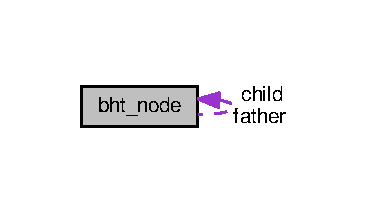
\includegraphics[width=178pt]{structbht__node__coll__graph}
\end{center}
\end{figure}
\subsection*{Data Fields}
\begin{DoxyCompactItemize}
\item 
double \hyperlink{structbht__node_ad4bd51cdbe6ba41894905207ed94974f}{len}
\item 
double \hyperlink{structbht__node_a9da2c4f10aed3a86628aad3dd87c9d6a}{center} \mbox{[}3\mbox{]}
\item 
int \hyperlink{structbht__node_a0c60ab00baa47c069768352b2f2b6d3d}{partnum}
\item 
struct \hyperlink{structbht__node}{bht\-\_\-node} $\ast$ \hyperlink{structbht__node_ad327b7e4aaac3a9687feb283d05fabbe}{father}
\item 
struct \hyperlink{structbht__node}{bht\-\_\-node} $\ast$ \hyperlink{structbht__node_a79d661ac20d812ad17b1d7455ad9e031}{child} \mbox{[}8\mbox{]}
\item 
unsigned char \hyperlink{structbht__node_afdde1540721b0d5dbc4b234677b4ad8d}{leaf}
\item 
unsigned char \hyperlink{structbht__node_a3aa7881ee7de66da41c4eeacb9280836}{isempty}
\end{DoxyCompactItemize}


\subsection{Detailed Description}


Definition at line 278 of file global.\-h.



\subsection{Field Documentation}
\hypertarget{structbht__node_a9da2c4f10aed3a86628aad3dd87c9d6a}{\index{bht\-\_\-node@{bht\-\_\-node}!center@{center}}
\index{center@{center}!bht_node@{bht\-\_\-node}}
\subsubsection[{center}]{\setlength{\rightskip}{0pt plus 5cm}double center\mbox{[}3\mbox{]}}}\label{structbht__node_a9da2c4f10aed3a86628aad3dd87c9d6a}


Definition at line 280 of file global.\-h.

\hypertarget{structbht__node_a79d661ac20d812ad17b1d7455ad9e031}{\index{bht\-\_\-node@{bht\-\_\-node}!child@{child}}
\index{child@{child}!bht_node@{bht\-\_\-node}}
\subsubsection[{child}]{\setlength{\rightskip}{0pt plus 5cm}struct {\bf bht\-\_\-node}$\ast$ child\mbox{[}8\mbox{]}}}\label{structbht__node_a79d661ac20d812ad17b1d7455ad9e031}


Definition at line 283 of file global.\-h.

\hypertarget{structbht__node_ad327b7e4aaac3a9687feb283d05fabbe}{\index{bht\-\_\-node@{bht\-\_\-node}!father@{father}}
\index{father@{father}!bht_node@{bht\-\_\-node}}
\subsubsection[{father}]{\setlength{\rightskip}{0pt plus 5cm}struct {\bf bht\-\_\-node}$\ast$ father}}\label{structbht__node_ad327b7e4aaac3a9687feb283d05fabbe}


Definition at line 282 of file global.\-h.

\hypertarget{structbht__node_a3aa7881ee7de66da41c4eeacb9280836}{\index{bht\-\_\-node@{bht\-\_\-node}!isempty@{isempty}}
\index{isempty@{isempty}!bht_node@{bht\-\_\-node}}
\subsubsection[{isempty}]{\setlength{\rightskip}{0pt plus 5cm}unsigned char isempty}}\label{structbht__node_a3aa7881ee7de66da41c4eeacb9280836}


Definition at line 285 of file global.\-h.

\hypertarget{structbht__node_afdde1540721b0d5dbc4b234677b4ad8d}{\index{bht\-\_\-node@{bht\-\_\-node}!leaf@{leaf}}
\index{leaf@{leaf}!bht_node@{bht\-\_\-node}}
\subsubsection[{leaf}]{\setlength{\rightskip}{0pt plus 5cm}unsigned char leaf}}\label{structbht__node_afdde1540721b0d5dbc4b234677b4ad8d}


Definition at line 284 of file global.\-h.

\hypertarget{structbht__node_ad4bd51cdbe6ba41894905207ed94974f}{\index{bht\-\_\-node@{bht\-\_\-node}!len@{len}}
\index{len@{len}!bht_node@{bht\-\_\-node}}
\subsubsection[{len}]{\setlength{\rightskip}{0pt plus 5cm}double len}}\label{structbht__node_ad4bd51cdbe6ba41894905207ed94974f}


Definition at line 279 of file global.\-h.

\hypertarget{structbht__node_a0c60ab00baa47c069768352b2f2b6d3d}{\index{bht\-\_\-node@{bht\-\_\-node}!partnum@{partnum}}
\index{partnum@{partnum}!bht_node@{bht\-\_\-node}}
\subsubsection[{partnum}]{\setlength{\rightskip}{0pt plus 5cm}int partnum}}\label{structbht__node_a0c60ab00baa47c069768352b2f2b6d3d}


Definition at line 281 of file global.\-h.



The documentation for this struct was generated from the following file\-:\begin{DoxyCompactItemize}
\item 
\hyperlink{global_8h}{global.\-h}\end{DoxyCompactItemize}

\hypertarget{structcellData}{\section{cell\-Data Struct Reference}
\label{structcellData}\index{cell\-Data@{cell\-Data}}
}


{\ttfamily \#include $<$global.\-h$>$}

\subsection*{Data Fields}
\begin{DoxyCompactItemize}
\item 
int \hyperlink{structcellData_ada4af333b662b0bba80e2f5e273fe4ea}{lifetime}
\item 
int \hyperlink{structcellData_accf3aec63bc20b3c99ab4881cb07c05b}{phase}
\item 
int \hyperlink{structcellData_a91d98a856bbd96810b40af3ca5cc901a}{age}
\item 
int \hyperlink{structcellData_add1e1533be6e693ffedcdbafdf8b855c}{death}
\item 
int \hyperlink{structcellData_a80ff3fcc4d03d0b1b01559839d12df5b}{halo}
\item 
float \hyperlink{structcellData_afe1297f954440c453b59fcb06992dbd5}{phasetime}
\item 
float \hyperlink{structcellData_a581debe7d16bce9d187b97855f4e99d4}{g1}
\item 
float \hyperlink{structcellData_a874f74a4dc1c9a0cd9c6e0d79c298f55}{s}
\item 
float \hyperlink{structcellData_aee9971139118d56815564304450c4775}{g2}
\item 
float \hyperlink{structcellData_ac51334f57ef8b81c0629c9421798c344}{m}
\item 
float \hyperlink{structcellData_ad0bd87a264e65d1c17ecc07049819f2c}{young}
\item 
Z\-O\-L\-T\-A\-N\-\_\-\-I\-D\-\_\-\-T\-Y\-P\-E \hyperlink{structcellData_abb4d4bd9231e9f994e87f32cc4fcfce8}{gid}
\item 
double \hyperlink{structcellData_af88b946fb90d5f08b5fb740c70e98c10}{x}
\item 
double \hyperlink{structcellData_ab927965981178aa1fba979a37168db2a}{y}
\item 
double \hyperlink{structcellData_ab3e6ed577a7c669c19de1f9c1b46c872}{z}
\item 
double \hyperlink{structcellData_aba3c5d750d5dbd6e86c11ecaca62885e}{size}
\item 
double \hyperlink{structcellData_a8ee9be1b5aa75abae556de3088cba6d9}{h}
\item 
double \hyperlink{structcellData_a3b90d5a73541ab9402511d87bed076ef}{v}
\item 
double \hyperlink{structcellData_a6f8c052f8417728038991f7f2826d38d}{density}
\item 
double \hyperlink{structcellData_a0045a5036d7f3f873fe33380932d4313}{scalar\-Field}
\item 
unsigned char \hyperlink{structcellData_a49af8c5336d6c2401bc24f86dbb97b36}{tumor}
\end{DoxyCompactItemize}


\subsection{Detailed Description}


Definition at line 56 of file global.\-h.



\subsection{Field Documentation}
\hypertarget{structcellData_a91d98a856bbd96810b40af3ca5cc901a}{\index{cell\-Data@{cell\-Data}!age@{age}}
\index{age@{age}!cellData@{cell\-Data}}
\subsubsection[{age}]{\setlength{\rightskip}{0pt plus 5cm}int age}}\label{structcellData_a91d98a856bbd96810b40af3ca5cc901a}


Definition at line 59 of file global.\-h.

\hypertarget{structcellData_add1e1533be6e693ffedcdbafdf8b855c}{\index{cell\-Data@{cell\-Data}!death@{death}}
\index{death@{death}!cellData@{cell\-Data}}
\subsubsection[{death}]{\setlength{\rightskip}{0pt plus 5cm}int death}}\label{structcellData_add1e1533be6e693ffedcdbafdf8b855c}


Definition at line 60 of file global.\-h.

\hypertarget{structcellData_a6f8c052f8417728038991f7f2826d38d}{\index{cell\-Data@{cell\-Data}!density@{density}}
\index{density@{density}!cellData@{cell\-Data}}
\subsubsection[{density}]{\setlength{\rightskip}{0pt plus 5cm}double density}}\label{structcellData_a6f8c052f8417728038991f7f2826d38d}


Definition at line 75 of file global.\-h.

\hypertarget{structcellData_a581debe7d16bce9d187b97855f4e99d4}{\index{cell\-Data@{cell\-Data}!g1@{g1}}
\index{g1@{g1}!cellData@{cell\-Data}}
\subsubsection[{g1}]{\setlength{\rightskip}{0pt plus 5cm}float g1}}\label{structcellData_a581debe7d16bce9d187b97855f4e99d4}


Definition at line 63 of file global.\-h.

\hypertarget{structcellData_aee9971139118d56815564304450c4775}{\index{cell\-Data@{cell\-Data}!g2@{g2}}
\index{g2@{g2}!cellData@{cell\-Data}}
\subsubsection[{g2}]{\setlength{\rightskip}{0pt plus 5cm}float g2}}\label{structcellData_aee9971139118d56815564304450c4775}


Definition at line 65 of file global.\-h.

\hypertarget{structcellData_abb4d4bd9231e9f994e87f32cc4fcfce8}{\index{cell\-Data@{cell\-Data}!gid@{gid}}
\index{gid@{gid}!cellData@{cell\-Data}}
\subsubsection[{gid}]{\setlength{\rightskip}{0pt plus 5cm}Z\-O\-L\-T\-A\-N\-\_\-\-I\-D\-\_\-\-T\-Y\-P\-E gid}}\label{structcellData_abb4d4bd9231e9f994e87f32cc4fcfce8}


Definition at line 68 of file global.\-h.

\hypertarget{structcellData_a8ee9be1b5aa75abae556de3088cba6d9}{\index{cell\-Data@{cell\-Data}!h@{h}}
\index{h@{h}!cellData@{cell\-Data}}
\subsubsection[{h}]{\setlength{\rightskip}{0pt plus 5cm}double h}}\label{structcellData_a8ee9be1b5aa75abae556de3088cba6d9}


Definition at line 73 of file global.\-h.

\hypertarget{structcellData_a80ff3fcc4d03d0b1b01559839d12df5b}{\index{cell\-Data@{cell\-Data}!halo@{halo}}
\index{halo@{halo}!cellData@{cell\-Data}}
\subsubsection[{halo}]{\setlength{\rightskip}{0pt plus 5cm}int halo}}\label{structcellData_a80ff3fcc4d03d0b1b01559839d12df5b}


Definition at line 61 of file global.\-h.

\hypertarget{structcellData_ada4af333b662b0bba80e2f5e273fe4ea}{\index{cell\-Data@{cell\-Data}!lifetime@{lifetime}}
\index{lifetime@{lifetime}!cellData@{cell\-Data}}
\subsubsection[{lifetime}]{\setlength{\rightskip}{0pt plus 5cm}int lifetime}}\label{structcellData_ada4af333b662b0bba80e2f5e273fe4ea}


Definition at line 57 of file global.\-h.

\hypertarget{structcellData_ac51334f57ef8b81c0629c9421798c344}{\index{cell\-Data@{cell\-Data}!m@{m}}
\index{m@{m}!cellData@{cell\-Data}}
\subsubsection[{m}]{\setlength{\rightskip}{0pt plus 5cm}float m}}\label{structcellData_ac51334f57ef8b81c0629c9421798c344}


Definition at line 66 of file global.\-h.

\hypertarget{structcellData_accf3aec63bc20b3c99ab4881cb07c05b}{\index{cell\-Data@{cell\-Data}!phase@{phase}}
\index{phase@{phase}!cellData@{cell\-Data}}
\subsubsection[{phase}]{\setlength{\rightskip}{0pt plus 5cm}int phase}}\label{structcellData_accf3aec63bc20b3c99ab4881cb07c05b}


Definition at line 58 of file global.\-h.

\hypertarget{structcellData_afe1297f954440c453b59fcb06992dbd5}{\index{cell\-Data@{cell\-Data}!phasetime@{phasetime}}
\index{phasetime@{phasetime}!cellData@{cell\-Data}}
\subsubsection[{phasetime}]{\setlength{\rightskip}{0pt plus 5cm}float phasetime}}\label{structcellData_afe1297f954440c453b59fcb06992dbd5}


Definition at line 62 of file global.\-h.

\hypertarget{structcellData_a874f74a4dc1c9a0cd9c6e0d79c298f55}{\index{cell\-Data@{cell\-Data}!s@{s}}
\index{s@{s}!cellData@{cell\-Data}}
\subsubsection[{s}]{\setlength{\rightskip}{0pt plus 5cm}float s}}\label{structcellData_a874f74a4dc1c9a0cd9c6e0d79c298f55}


Definition at line 64 of file global.\-h.

\hypertarget{structcellData_a0045a5036d7f3f873fe33380932d4313}{\index{cell\-Data@{cell\-Data}!scalar\-Field@{scalar\-Field}}
\index{scalar\-Field@{scalar\-Field}!cellData@{cell\-Data}}
\subsubsection[{scalar\-Field}]{\setlength{\rightskip}{0pt plus 5cm}double scalar\-Field}}\label{structcellData_a0045a5036d7f3f873fe33380932d4313}


Definition at line 76 of file global.\-h.

\hypertarget{structcellData_aba3c5d750d5dbd6e86c11ecaca62885e}{\index{cell\-Data@{cell\-Data}!size@{size}}
\index{size@{size}!cellData@{cell\-Data}}
\subsubsection[{size}]{\setlength{\rightskip}{0pt plus 5cm}double size}}\label{structcellData_aba3c5d750d5dbd6e86c11ecaca62885e}


Definition at line 72 of file global.\-h.

\hypertarget{structcellData_a49af8c5336d6c2401bc24f86dbb97b36}{\index{cell\-Data@{cell\-Data}!tumor@{tumor}}
\index{tumor@{tumor}!cellData@{cell\-Data}}
\subsubsection[{tumor}]{\setlength{\rightskip}{0pt plus 5cm}unsigned char tumor}}\label{structcellData_a49af8c5336d6c2401bc24f86dbb97b36}


Definition at line 77 of file global.\-h.

\hypertarget{structcellData_a3b90d5a73541ab9402511d87bed076ef}{\index{cell\-Data@{cell\-Data}!v@{v}}
\index{v@{v}!cellData@{cell\-Data}}
\subsubsection[{v}]{\setlength{\rightskip}{0pt plus 5cm}double v}}\label{structcellData_a3b90d5a73541ab9402511d87bed076ef}


Definition at line 74 of file global.\-h.

\hypertarget{structcellData_af88b946fb90d5f08b5fb740c70e98c10}{\index{cell\-Data@{cell\-Data}!x@{x}}
\index{x@{x}!cellData@{cell\-Data}}
\subsubsection[{x}]{\setlength{\rightskip}{0pt plus 5cm}double x}}\label{structcellData_af88b946fb90d5f08b5fb740c70e98c10}


Definition at line 69 of file global.\-h.

\hypertarget{structcellData_ab927965981178aa1fba979a37168db2a}{\index{cell\-Data@{cell\-Data}!y@{y}}
\index{y@{y}!cellData@{cell\-Data}}
\subsubsection[{y}]{\setlength{\rightskip}{0pt plus 5cm}double y}}\label{structcellData_ab927965981178aa1fba979a37168db2a}


Definition at line 70 of file global.\-h.

\hypertarget{structcellData_ad0bd87a264e65d1c17ecc07049819f2c}{\index{cell\-Data@{cell\-Data}!young@{young}}
\index{young@{young}!cellData@{cell\-Data}}
\subsubsection[{young}]{\setlength{\rightskip}{0pt plus 5cm}float young}}\label{structcellData_ad0bd87a264e65d1c17ecc07049819f2c}


Definition at line 67 of file global.\-h.

\hypertarget{structcellData_ab3e6ed577a7c669c19de1f9c1b46c872}{\index{cell\-Data@{cell\-Data}!z@{z}}
\index{z@{z}!cellData@{cell\-Data}}
\subsubsection[{z}]{\setlength{\rightskip}{0pt plus 5cm}double z}}\label{structcellData_ab3e6ed577a7c669c19de1f9c1b46c872}


Definition at line 71 of file global.\-h.



The documentation for this struct was generated from the following file\-:\begin{DoxyCompactItemize}
\item 
\hyperlink{global_8h}{global.\-h}\end{DoxyCompactItemize}

\hypertarget{structcolormap__t}{\section{colormap\-\_\-t Struct Reference}
\label{structcolormap__t}\index{colormap\-\_\-t@{colormap\-\_\-t}}
}


{\ttfamily \#include $<$io.\-h$>$}



Collaboration diagram for colormap\-\_\-t\-:\nopagebreak
\begin{figure}[H]
\begin{center}
\leavevmode
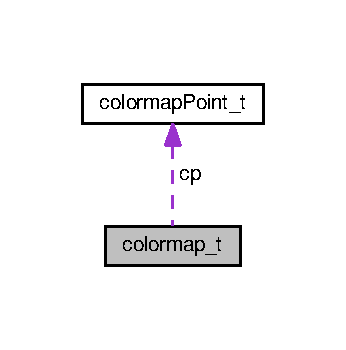
\includegraphics[width=166pt]{structcolormap__t__coll__graph}
\end{center}
\end{figure}
\subsection*{Data Fields}
\begin{DoxyCompactItemize}
\item 
char \hyperlink{structcolormap__t_acd328517a6cf718155c2e6e22b671ca9}{name} \mbox{[}16\mbox{]}
\item 
int \hyperlink{structcolormap__t_a8f4ec518913edf916c0dc3cbb49991b7}{ncp}
\item 
\hyperlink{io_8h_a2bf5ae344b8526b236f7152ce0424670}{colormap\-Point} $\ast$ \hyperlink{structcolormap__t_a64cbb09ad4367b201326341a4b500844}{cp}
\end{DoxyCompactItemize}


\subsection{Detailed Description}


Definition at line 96 of file io.\-h.



\subsection{Field Documentation}
\hypertarget{structcolormap__t_a64cbb09ad4367b201326341a4b500844}{\index{colormap\-\_\-t@{colormap\-\_\-t}!cp@{cp}}
\index{cp@{cp}!colormap_t@{colormap\-\_\-t}}
\subsubsection[{cp}]{\setlength{\rightskip}{0pt plus 5cm}{\bf colormap\-Point}$\ast$ cp}}\label{structcolormap__t_a64cbb09ad4367b201326341a4b500844}


Definition at line 99 of file io.\-h.

\hypertarget{structcolormap__t_acd328517a6cf718155c2e6e22b671ca9}{\index{colormap\-\_\-t@{colormap\-\_\-t}!name@{name}}
\index{name@{name}!colormap_t@{colormap\-\_\-t}}
\subsubsection[{name}]{\setlength{\rightskip}{0pt plus 5cm}char name\mbox{[}16\mbox{]}}}\label{structcolormap__t_acd328517a6cf718155c2e6e22b671ca9}


Definition at line 97 of file io.\-h.

\hypertarget{structcolormap__t_a8f4ec518913edf916c0dc3cbb49991b7}{\index{colormap\-\_\-t@{colormap\-\_\-t}!ncp@{ncp}}
\index{ncp@{ncp}!colormap_t@{colormap\-\_\-t}}
\subsubsection[{ncp}]{\setlength{\rightskip}{0pt plus 5cm}int ncp}}\label{structcolormap__t_a8f4ec518913edf916c0dc3cbb49991b7}


Definition at line 98 of file io.\-h.



The documentation for this struct was generated from the following file\-:\begin{DoxyCompactItemize}
\item 
\hyperlink{io_8h}{io.\-h}\end{DoxyCompactItemize}

\hypertarget{structcolormapPoint__t}{\section{colormap\-Point\-\_\-t Struct Reference}
\label{structcolormapPoint__t}\index{colormap\-Point\-\_\-t@{colormap\-Point\-\_\-t}}
}


{\ttfamily \#include $<$io.\-h$>$}

\subsection*{Data Fields}
\begin{DoxyCompactItemize}
\item 
float \hyperlink{structcolormapPoint__t_a76777b356ab2a080225682528119c4fe}{position}
\item 
float \hyperlink{structcolormapPoint__t_a4788d82c901b9367dd5c0daff8a7616b}{r}
\item 
float \hyperlink{structcolormapPoint__t_a8cf17d727651616de6f2b79ef32170cd}{g}
\item 
float \hyperlink{structcolormapPoint__t_a83fc1af92e29717b4513d121b0c72c7d}{b}
\end{DoxyCompactItemize}


\subsection{Detailed Description}


Definition at line 89 of file io.\-h.



\subsection{Field Documentation}
\hypertarget{structcolormapPoint__t_a83fc1af92e29717b4513d121b0c72c7d}{\index{colormap\-Point\-\_\-t@{colormap\-Point\-\_\-t}!b@{b}}
\index{b@{b}!colormapPoint_t@{colormap\-Point\-\_\-t}}
\subsubsection[{b}]{\setlength{\rightskip}{0pt plus 5cm}float b}}\label{structcolormapPoint__t_a83fc1af92e29717b4513d121b0c72c7d}


Definition at line 93 of file io.\-h.

\hypertarget{structcolormapPoint__t_a8cf17d727651616de6f2b79ef32170cd}{\index{colormap\-Point\-\_\-t@{colormap\-Point\-\_\-t}!g@{g}}
\index{g@{g}!colormapPoint_t@{colormap\-Point\-\_\-t}}
\subsubsection[{g}]{\setlength{\rightskip}{0pt plus 5cm}float g}}\label{structcolormapPoint__t_a8cf17d727651616de6f2b79ef32170cd}


Definition at line 92 of file io.\-h.

\hypertarget{structcolormapPoint__t_a76777b356ab2a080225682528119c4fe}{\index{colormap\-Point\-\_\-t@{colormap\-Point\-\_\-t}!position@{position}}
\index{position@{position}!colormapPoint_t@{colormap\-Point\-\_\-t}}
\subsubsection[{position}]{\setlength{\rightskip}{0pt plus 5cm}float position}}\label{structcolormapPoint__t_a76777b356ab2a080225682528119c4fe}


Definition at line 90 of file io.\-h.

\hypertarget{structcolormapPoint__t_a4788d82c901b9367dd5c0daff8a7616b}{\index{colormap\-Point\-\_\-t@{colormap\-Point\-\_\-t}!r@{r}}
\index{r@{r}!colormapPoint_t@{colormap\-Point\-\_\-t}}
\subsubsection[{r}]{\setlength{\rightskip}{0pt plus 5cm}float r}}\label{structcolormapPoint__t_a4788d82c901b9367dd5c0daff8a7616b}


Definition at line 91 of file io.\-h.



The documentation for this struct was generated from the following file\-:\begin{DoxyCompactItemize}
\item 
\hyperlink{io_8h}{io.\-h}\end{DoxyCompactItemize}

\hypertarget{structdensPotData}{\section{dens\-Pot\-Data Struct Reference}
\label{structdensPotData}\index{dens\-Pot\-Data@{dens\-Pot\-Data}}
}


{\ttfamily \#include $<$global.\-h$>$}

\subsection*{Data Fields}
\begin{DoxyCompactItemize}
\item 
double \hyperlink{structdensPotData_a3b90d5a73541ab9402511d87bed076ef}{v}
\item 
double \hyperlink{structdensPotData_a6f8c052f8417728038991f7f2826d38d}{density}
\end{DoxyCompactItemize}


\subsection{Detailed Description}


Definition at line 126 of file global.\-h.



\subsection{Field Documentation}
\hypertarget{structdensPotData_a6f8c052f8417728038991f7f2826d38d}{\index{dens\-Pot\-Data@{dens\-Pot\-Data}!density@{density}}
\index{density@{density}!densPotData@{dens\-Pot\-Data}}
\subsubsection[{density}]{\setlength{\rightskip}{0pt plus 5cm}double density}}\label{structdensPotData_a6f8c052f8417728038991f7f2826d38d}


Definition at line 128 of file global.\-h.

\hypertarget{structdensPotData_a3b90d5a73541ab9402511d87bed076ef}{\index{dens\-Pot\-Data@{dens\-Pot\-Data}!v@{v}}
\index{v@{v}!densPotData@{dens\-Pot\-Data}}
\subsubsection[{v}]{\setlength{\rightskip}{0pt plus 5cm}double v}}\label{structdensPotData_a3b90d5a73541ab9402511d87bed076ef}


Definition at line 127 of file global.\-h.



The documentation for this struct was generated from the following file\-:\begin{DoxyCompactItemize}
\item 
\hyperlink{global_8h}{global.\-h}\end{DoxyCompactItemize}

\hypertarget{structdoubleVector3d}{\section{double\-Vector3d Struct Reference}
\label{structdoubleVector3d}\index{double\-Vector3d@{double\-Vector3d}}
}


{\ttfamily \#include $<$global.\-h$>$}

\subsection*{Data Fields}
\begin{DoxyCompactItemize}
\item 
double \hyperlink{structdoubleVector3d_af88b946fb90d5f08b5fb740c70e98c10}{x}
\item 
double \hyperlink{structdoubleVector3d_ab927965981178aa1fba979a37168db2a}{y}
\item 
double \hyperlink{structdoubleVector3d_ab3e6ed577a7c669c19de1f9c1b46c872}{z}
\end{DoxyCompactItemize}


\subsection{Detailed Description}


Definition at line 222 of file global.\-h.



\subsection{Field Documentation}
\hypertarget{structdoubleVector3d_af88b946fb90d5f08b5fb740c70e98c10}{\index{double\-Vector3d@{double\-Vector3d}!x@{x}}
\index{x@{x}!doubleVector3d@{double\-Vector3d}}
\subsubsection[{x}]{\setlength{\rightskip}{0pt plus 5cm}double x}}\label{structdoubleVector3d_af88b946fb90d5f08b5fb740c70e98c10}


Definition at line 223 of file global.\-h.

\hypertarget{structdoubleVector3d_ab927965981178aa1fba979a37168db2a}{\index{double\-Vector3d@{double\-Vector3d}!y@{y}}
\index{y@{y}!doubleVector3d@{double\-Vector3d}}
\subsubsection[{y}]{\setlength{\rightskip}{0pt plus 5cm}double y}}\label{structdoubleVector3d_ab927965981178aa1fba979a37168db2a}


Definition at line 224 of file global.\-h.

\hypertarget{structdoubleVector3d_ab3e6ed577a7c669c19de1f9c1b46c872}{\index{double\-Vector3d@{double\-Vector3d}!z@{z}}
\index{z@{z}!doubleVector3d@{double\-Vector3d}}
\subsubsection[{z}]{\setlength{\rightskip}{0pt plus 5cm}double z}}\label{structdoubleVector3d_ab3e6ed577a7c669c19de1f9c1b46c872}


Definition at line 225 of file global.\-h.



The documentation for this struct was generated from the following file\-:\begin{DoxyCompactItemize}
\item 
\hyperlink{global_8h}{global.\-h}\end{DoxyCompactItemize}

\hypertarget{structexpData}{\section{exp\-Data Struct Reference}
\label{structexpData}\index{exp\-Data@{exp\-Data}}
}
\subsection*{Data Fields}
\begin{DoxyCompactItemize}
\item 
int \hyperlink{structexpData_af00601a22186810a9e6d16efb75862ce}{cell}
\item 
int \hyperlink{structexpData_a7e9d757c9982bd721d598bad366fbe62}{proc}
\end{DoxyCompactItemize}


\subsection{Detailed Description}


Definition at line 32 of file comm.\-c.



\subsection{Field Documentation}
\hypertarget{structexpData_af00601a22186810a9e6d16efb75862ce}{\index{exp\-Data@{exp\-Data}!cell@{cell}}
\index{cell@{cell}!expData@{exp\-Data}}
\subsubsection[{cell}]{\setlength{\rightskip}{0pt plus 5cm}int cell}}\label{structexpData_af00601a22186810a9e6d16efb75862ce}


Definition at line 33 of file comm.\-c.

\hypertarget{structexpData_a7e9d757c9982bd721d598bad366fbe62}{\index{exp\-Data@{exp\-Data}!proc@{proc}}
\index{proc@{proc}!expData@{exp\-Data}}
\subsubsection[{proc}]{\setlength{\rightskip}{0pt plus 5cm}int proc}}\label{structexpData_a7e9d757c9982bd721d598bad366fbe62}


Definition at line 34 of file comm.\-c.



The documentation for this struct was generated from the following file\-:\begin{DoxyCompactItemize}
\item 
\hyperlink{comm_8c}{comm.\-c}\end{DoxyCompactItemize}

\hypertarget{structfloatVector3d}{\section{float\-Vector3d Struct Reference}
\label{structfloatVector3d}\index{float\-Vector3d@{float\-Vector3d}}
}


{\ttfamily \#include $<$global.\-h$>$}

\subsection*{Data Fields}
\begin{DoxyCompactItemize}
\item 
float \hyperlink{structfloatVector3d_ad0da36b2558901e21e7a30f6c227a45e}{x}
\item 
float \hyperlink{structfloatVector3d_aa4f0d3eebc3c443f9be81bf48561a217}{y}
\item 
float \hyperlink{structfloatVector3d_af73583b1e980b0aa03f9884812e9fd4d}{z}
\end{DoxyCompactItemize}


\subsection{Detailed Description}


Definition at line 234 of file global.\-h.



\subsection{Field Documentation}
\hypertarget{structfloatVector3d_ad0da36b2558901e21e7a30f6c227a45e}{\index{float\-Vector3d@{float\-Vector3d}!x@{x}}
\index{x@{x}!floatVector3d@{float\-Vector3d}}
\subsubsection[{x}]{\setlength{\rightskip}{0pt plus 5cm}float x}}\label{structfloatVector3d_ad0da36b2558901e21e7a30f6c227a45e}


Definition at line 235 of file global.\-h.

\hypertarget{structfloatVector3d_aa4f0d3eebc3c443f9be81bf48561a217}{\index{float\-Vector3d@{float\-Vector3d}!y@{y}}
\index{y@{y}!floatVector3d@{float\-Vector3d}}
\subsubsection[{y}]{\setlength{\rightskip}{0pt plus 5cm}float y}}\label{structfloatVector3d_aa4f0d3eebc3c443f9be81bf48561a217}


Definition at line 236 of file global.\-h.

\hypertarget{structfloatVector3d_af73583b1e980b0aa03f9884812e9fd4d}{\index{float\-Vector3d@{float\-Vector3d}!z@{z}}
\index{z@{z}!floatVector3d@{float\-Vector3d}}
\subsubsection[{z}]{\setlength{\rightskip}{0pt plus 5cm}float z}}\label{structfloatVector3d_af73583b1e980b0aa03f9884812e9fd4d}


Definition at line 237 of file global.\-h.



The documentation for this struct was generated from the following file\-:\begin{DoxyCompactItemize}
\item 
\hyperlink{global_8h}{global.\-h}\end{DoxyCompactItemize}

\hypertarget{structint64Vector3d}{\section{int64\-Vector3d Struct Reference}
\label{structint64Vector3d}\index{int64\-Vector3d@{int64\-Vector3d}}
}


{\ttfamily \#include $<$global.\-h$>$}

\subsection*{Data Fields}
\begin{DoxyCompactItemize}
\item 
int64\-\_\-t \hyperlink{structint64Vector3d_a040359f45343ce6667f5c66fda5f50e3}{x}
\item 
int64\-\_\-t \hyperlink{structint64Vector3d_a0cbcba26311a97b8e0763317e105a918}{y}
\item 
int64\-\_\-t \hyperlink{structint64Vector3d_a44624880ae3bb63041297b70cb33408b}{z}
\end{DoxyCompactItemize}


\subsection{Detailed Description}


Definition at line 228 of file global.\-h.



\subsection{Field Documentation}
\hypertarget{structint64Vector3d_a040359f45343ce6667f5c66fda5f50e3}{\index{int64\-Vector3d@{int64\-Vector3d}!x@{x}}
\index{x@{x}!int64Vector3d@{int64\-Vector3d}}
\subsubsection[{x}]{\setlength{\rightskip}{0pt plus 5cm}int64\-\_\-t x}}\label{structint64Vector3d_a040359f45343ce6667f5c66fda5f50e3}


Definition at line 229 of file global.\-h.

\hypertarget{structint64Vector3d_a0cbcba26311a97b8e0763317e105a918}{\index{int64\-Vector3d@{int64\-Vector3d}!y@{y}}
\index{y@{y}!int64Vector3d@{int64\-Vector3d}}
\subsubsection[{y}]{\setlength{\rightskip}{0pt plus 5cm}int64\-\_\-t y}}\label{structint64Vector3d_a0cbcba26311a97b8e0763317e105a918}


Definition at line 230 of file global.\-h.

\hypertarget{structint64Vector3d_a44624880ae3bb63041297b70cb33408b}{\index{int64\-Vector3d@{int64\-Vector3d}!z@{z}}
\index{z@{z}!int64Vector3d@{int64\-Vector3d}}
\subsubsection[{z}]{\setlength{\rightskip}{0pt plus 5cm}int64\-\_\-t z}}\label{structint64Vector3d_a44624880ae3bb63041297b70cb33408b}


Definition at line 231 of file global.\-h.



The documentation for this struct was generated from the following file\-:\begin{DoxyCompactItemize}
\item 
\hyperlink{global_8h}{global.\-h}\end{DoxyCompactItemize}

\hypertarget{structpartData}{\section{part\-Data Struct Reference}
\label{structpartData}\index{part\-Data@{part\-Data}}
}


{\ttfamily \#include $<$global.\-h$>$}

\subsection*{Data Fields}
\begin{DoxyCompactItemize}
\item 
double \hyperlink{structpartData_af88b946fb90d5f08b5fb740c70e98c10}{x}
\item 
double \hyperlink{structpartData_ab927965981178aa1fba979a37168db2a}{y}
\item 
double \hyperlink{structpartData_ab3e6ed577a7c669c19de1f9c1b46c872}{z}
\item 
double \hyperlink{structpartData_a8ee9be1b5aa75abae556de3088cba6d9}{h}
\item 
double \hyperlink{structpartData_aba3c5d750d5dbd6e86c11ecaca62885e}{size}
\item 
double \hyperlink{structpartData_a47ec3689b1fd89ba8e75d9a9975ba63f}{young}
\end{DoxyCompactItemize}


\subsection{Detailed Description}


Definition at line 116 of file global.\-h.



\subsection{Field Documentation}
\hypertarget{structpartData_a8ee9be1b5aa75abae556de3088cba6d9}{\index{part\-Data@{part\-Data}!h@{h}}
\index{h@{h}!partData@{part\-Data}}
\subsubsection[{h}]{\setlength{\rightskip}{0pt plus 5cm}double h}}\label{structpartData_a8ee9be1b5aa75abae556de3088cba6d9}


Definition at line 120 of file global.\-h.

\hypertarget{structpartData_aba3c5d750d5dbd6e86c11ecaca62885e}{\index{part\-Data@{part\-Data}!size@{size}}
\index{size@{size}!partData@{part\-Data}}
\subsubsection[{size}]{\setlength{\rightskip}{0pt plus 5cm}double size}}\label{structpartData_aba3c5d750d5dbd6e86c11ecaca62885e}


Definition at line 121 of file global.\-h.

\hypertarget{structpartData_af88b946fb90d5f08b5fb740c70e98c10}{\index{part\-Data@{part\-Data}!x@{x}}
\index{x@{x}!partData@{part\-Data}}
\subsubsection[{x}]{\setlength{\rightskip}{0pt plus 5cm}double x}}\label{structpartData_af88b946fb90d5f08b5fb740c70e98c10}


Definition at line 117 of file global.\-h.

\hypertarget{structpartData_ab927965981178aa1fba979a37168db2a}{\index{part\-Data@{part\-Data}!y@{y}}
\index{y@{y}!partData@{part\-Data}}
\subsubsection[{y}]{\setlength{\rightskip}{0pt plus 5cm}double y}}\label{structpartData_ab927965981178aa1fba979a37168db2a}


Definition at line 118 of file global.\-h.

\hypertarget{structpartData_a47ec3689b1fd89ba8e75d9a9975ba63f}{\index{part\-Data@{part\-Data}!young@{young}}
\index{young@{young}!partData@{part\-Data}}
\subsubsection[{young}]{\setlength{\rightskip}{0pt plus 5cm}double young}}\label{structpartData_a47ec3689b1fd89ba8e75d9a9975ba63f}


Definition at line 122 of file global.\-h.

\hypertarget{structpartData_ab3e6ed577a7c669c19de1f9c1b46c872}{\index{part\-Data@{part\-Data}!z@{z}}
\index{z@{z}!partData@{part\-Data}}
\subsubsection[{z}]{\setlength{\rightskip}{0pt plus 5cm}double z}}\label{structpartData_ab3e6ed577a7c669c19de1f9c1b46c872}


Definition at line 119 of file global.\-h.



The documentation for this struct was generated from the following file\-:\begin{DoxyCompactItemize}
\item 
\hyperlink{global_8h}{global.\-h}\end{DoxyCompactItemize}

\hypertarget{structstatisticsData}{\section{statistics\-Data Struct Reference}
\label{structstatisticsData}\index{statistics\-Data@{statistics\-Data}}
}


{\ttfamily \#include $<$global.\-h$>$}

\subsection*{Data Fields}
\begin{DoxyCompactItemize}
\item 
double \hyperlink{structstatisticsData_ad99dc4104d1898b6e593bbf331e41c69}{minsize}
\item 
double \hyperlink{structstatisticsData_a7383c898fd4cd4d862ca65d3713086cd}{maxsize}
\item 
double \hyperlink{structstatisticsData_a78455d23ec97258967b76cbb2332b7be}{mindist}
\item 
double \hyperlink{structstatisticsData_a485292d20f5d14bd18e83fef65976fb4}{maxvel}
\item 
double \hyperlink{structstatisticsData_a1b9d00ac67b4ceca8e7747a50edc802b}{minvel}
\item 
double \hyperlink{structstatisticsData_abc8b83844f3405d9046189aa841b48fd}{maxdens}
\item 
double \hyperlink{structstatisticsData_a2ddb05b9ae611dab07eef62db427ed61}{mindens}
\item 
double \hyperlink{structstatisticsData_a62a3935a35dda8e375bf0ec6cc160d5e}{densdev}
\item 
double \hyperlink{structstatisticsData_ae897d6b29710ca63a31e17866c73bc9a}{densavg}
\end{DoxyCompactItemize}


\subsection{Detailed Description}


Definition at line 256 of file global.\-h.



\subsection{Field Documentation}
\hypertarget{structstatisticsData_ae897d6b29710ca63a31e17866c73bc9a}{\index{statistics\-Data@{statistics\-Data}!densavg@{densavg}}
\index{densavg@{densavg}!statisticsData@{statistics\-Data}}
\subsubsection[{densavg}]{\setlength{\rightskip}{0pt plus 5cm}double densavg}}\label{structstatisticsData_ae897d6b29710ca63a31e17866c73bc9a}


Definition at line 265 of file global.\-h.

\hypertarget{structstatisticsData_a62a3935a35dda8e375bf0ec6cc160d5e}{\index{statistics\-Data@{statistics\-Data}!densdev@{densdev}}
\index{densdev@{densdev}!statisticsData@{statistics\-Data}}
\subsubsection[{densdev}]{\setlength{\rightskip}{0pt plus 5cm}double densdev}}\label{structstatisticsData_a62a3935a35dda8e375bf0ec6cc160d5e}


Definition at line 264 of file global.\-h.

\hypertarget{structstatisticsData_abc8b83844f3405d9046189aa841b48fd}{\index{statistics\-Data@{statistics\-Data}!maxdens@{maxdens}}
\index{maxdens@{maxdens}!statisticsData@{statistics\-Data}}
\subsubsection[{maxdens}]{\setlength{\rightskip}{0pt plus 5cm}double maxdens}}\label{structstatisticsData_abc8b83844f3405d9046189aa841b48fd}


Definition at line 262 of file global.\-h.

\hypertarget{structstatisticsData_a7383c898fd4cd4d862ca65d3713086cd}{\index{statistics\-Data@{statistics\-Data}!maxsize@{maxsize}}
\index{maxsize@{maxsize}!statisticsData@{statistics\-Data}}
\subsubsection[{maxsize}]{\setlength{\rightskip}{0pt plus 5cm}double maxsize}}\label{structstatisticsData_a7383c898fd4cd4d862ca65d3713086cd}


Definition at line 258 of file global.\-h.

\hypertarget{structstatisticsData_a485292d20f5d14bd18e83fef65976fb4}{\index{statistics\-Data@{statistics\-Data}!maxvel@{maxvel}}
\index{maxvel@{maxvel}!statisticsData@{statistics\-Data}}
\subsubsection[{maxvel}]{\setlength{\rightskip}{0pt plus 5cm}double maxvel}}\label{structstatisticsData_a485292d20f5d14bd18e83fef65976fb4}


Definition at line 260 of file global.\-h.

\hypertarget{structstatisticsData_a2ddb05b9ae611dab07eef62db427ed61}{\index{statistics\-Data@{statistics\-Data}!mindens@{mindens}}
\index{mindens@{mindens}!statisticsData@{statistics\-Data}}
\subsubsection[{mindens}]{\setlength{\rightskip}{0pt plus 5cm}double mindens}}\label{structstatisticsData_a2ddb05b9ae611dab07eef62db427ed61}


Definition at line 263 of file global.\-h.

\hypertarget{structstatisticsData_a78455d23ec97258967b76cbb2332b7be}{\index{statistics\-Data@{statistics\-Data}!mindist@{mindist}}
\index{mindist@{mindist}!statisticsData@{statistics\-Data}}
\subsubsection[{mindist}]{\setlength{\rightskip}{0pt plus 5cm}double mindist}}\label{structstatisticsData_a78455d23ec97258967b76cbb2332b7be}


Definition at line 259 of file global.\-h.

\hypertarget{structstatisticsData_ad99dc4104d1898b6e593bbf331e41c69}{\index{statistics\-Data@{statistics\-Data}!minsize@{minsize}}
\index{minsize@{minsize}!statisticsData@{statistics\-Data}}
\subsubsection[{minsize}]{\setlength{\rightskip}{0pt plus 5cm}double minsize}}\label{structstatisticsData_ad99dc4104d1898b6e593bbf331e41c69}


Definition at line 257 of file global.\-h.

\hypertarget{structstatisticsData_a1b9d00ac67b4ceca8e7747a50edc802b}{\index{statistics\-Data@{statistics\-Data}!minvel@{minvel}}
\index{minvel@{minvel}!statisticsData@{statistics\-Data}}
\subsubsection[{minvel}]{\setlength{\rightskip}{0pt plus 5cm}double minvel}}\label{structstatisticsData_a1b9d00ac67b4ceca8e7747a50edc802b}


Definition at line 261 of file global.\-h.



The documentation for this struct was generated from the following file\-:\begin{DoxyCompactItemize}
\item 
\hyperlink{global_8h}{global.\-h}\end{DoxyCompactItemize}

\chapter{File Documentation}
\hypertarget{cells_8c}{\section{cells.\-c File Reference}
\label{cells_8c}\index{cells.\-c@{cells.\-c}}
}


contains functions which control current states and evolution of cells  


{\ttfamily \#include $<$stdio.\-h$>$}\\*
{\ttfamily \#include $<$stdlib.\-h$>$}\\*
{\ttfamily \#include $<$mpi.\-h$>$}\\*
{\ttfamily \#include $<$math.\-h$>$}\\*
{\ttfamily \#include $<$inttypes.\-h$>$}\\*
{\ttfamily \#include $<$sprng.\-h$>$}\\*
{\ttfamily \#include \char`\"{}global.\-h\char`\"{}}\\*
{\ttfamily \#include \char`\"{}inline.\-h\char`\"{}}\\*
{\ttfamily \#include \char`\"{}fields.\-h\char`\"{}}\\*
Include dependency graph for cells.\-c\-:\nopagebreak
\begin{figure}[H]
\begin{center}
\leavevmode
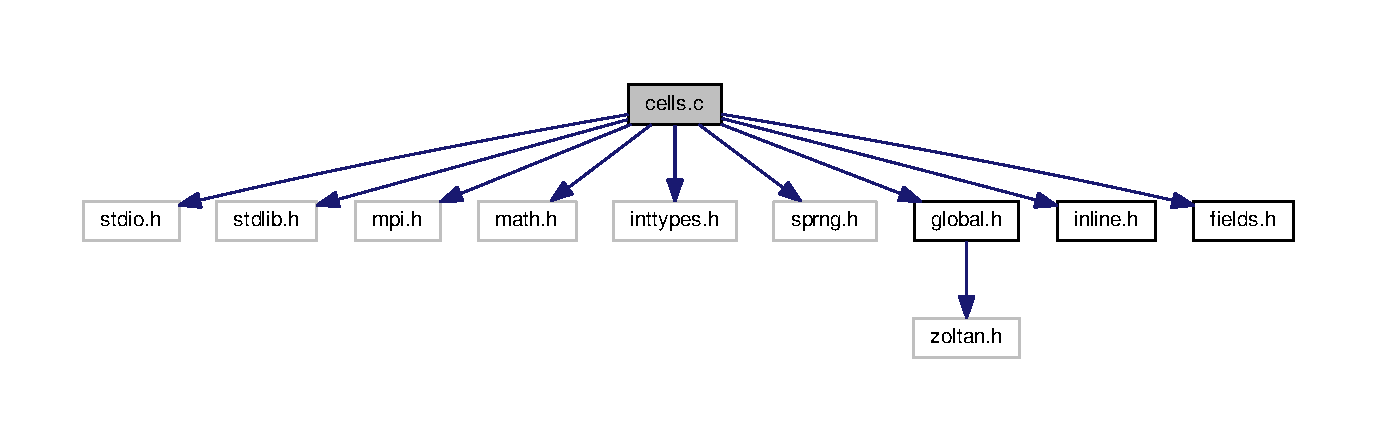
\includegraphics[width=350pt]{cells_8c__incl}
\end{center}
\end{figure}
\subsection*{Functions}
\begin{DoxyCompactItemize}
\item 
void \hyperlink{cells_8c_afdf0714d4b325131b21a0cbe42c44ece}{cells\-Allocate} ()
\item 
void \hyperlink{cells_8c_aa2527c8374034b85c4e95b665786b0ca}{cells\-Cycle\-Init} ()
\item 
int \hyperlink{cells_8c_a68e70197591e819d22315879c8141bdd}{cells\-Random\-Init} ()
\item 
void \hyperlink{cells_8c_a2d9450bd2eebb8f4d645417b92666b87}{mitosis} (int c)
\item 
void \hyperlink{cells_8c_a00dbe1f9f23fc7385462c32b89d28cf8}{mark\-Middle\-Cancer\-Cell} ()
\item 
void \hyperlink{cells_8c_aead37c061c3f1ec47259afaf2783029f}{cells\-Cleanup} ()
\item 
void \hyperlink{cells_8c_a8101c456dae07ab9cbd918ccad3a2ff7}{cells\-Death} (int lnc\-\_\-old)
\item 
void \hyperlink{cells_8c_aeeb6dee9938af6fef987f1c949458703}{update\-Cell\-Counters} ()
\item 
void \hyperlink{cells_8c_a227256c7da11efa2b4eacedf0a9f37c8}{update\-Cell\-Positions} ()
\item 
int \hyperlink{cells_8c_a718a88fce87f8ebdb87ed2fafed4c5c4}{update\-Cell\-Cycles} ()
\item 
void \hyperlink{cells_8c_aa2ee543811c23ee4b487102bb71ba9c7}{additional\-Scalar\-Field} ()
\item 
void \hyperlink{cells_8c_aeb1f066ef0713a8a50eb1e58784a3d7b}{update\-Cell\-States} ()
\end{DoxyCompactItemize}
\subsection*{Variables}
\begin{DoxyCompactItemize}
\item 
unsigned char $\ast$ \hyperlink{cells_8c_a96a825c021fe648b7fb171bd2c532ffb}{celld}
\end{DoxyCompactItemize}


\subsection{Detailed Description}
contains functions which control current states and evolution of cells 

Definition in file \hyperlink{cells_8c_source}{cells.\-c}.



\subsection{Function Documentation}
\hypertarget{cells_8c_aa2ee543811c23ee4b487102bb71ba9c7}{\index{cells.\-c@{cells.\-c}!additional\-Scalar\-Field@{additional\-Scalar\-Field}}
\index{additional\-Scalar\-Field@{additional\-Scalar\-Field}!cells.c@{cells.\-c}}
\subsubsection[{additional\-Scalar\-Field}]{\setlength{\rightskip}{0pt plus 5cm}void additional\-Scalar\-Field (
\begin{DoxyParamCaption}
{}
\end{DoxyParamCaption}
)}}\label{cells_8c_aa2ee543811c23ee4b487102bb71ba9c7}
This function fills the scalar\-Output field of each cell. It can be modified to output any float scalars that user would like to analyze or visualize after simulation. This field is printed to the output V\-T\-K files. 

Definition at line 704 of file cells.\-c.



References cells, cell\-Data\-::density, lnc, and cell\-Data\-::scalar\-Field.


\begin{DoxyCode}
705 \{
706   \textcolor{keywordtype}{int} c;
707   \textcolor{keywordflow}{for} (c = 0; c < \hyperlink{global_8h_a7065c019590815f10169c219f358e7d0}{lnc}; c++) \{
708     \textcolor{keywordflow}{if} (\hyperlink{global_8h_a56da06a03aa369ca203be968cb56d16c}{cells}[c].tumor == 1)
709       \hyperlink{global_8h_a56da06a03aa369ca203be968cb56d16c}{cells}[c].\hyperlink{structcellData_a0045a5036d7f3f873fe33380932d4313}{scalarField} = 8.0;
710     \textcolor{keywordflow}{else}
711       \hyperlink{global_8h_a56da06a03aa369ca203be968cb56d16c}{cells}[c].\hyperlink{structcellData_a0045a5036d7f3f873fe33380932d4313}{scalarField} = \hyperlink{global_8h_a56da06a03aa369ca203be968cb56d16c}{cells}[c].\hyperlink{structcellData_a6f8c052f8417728038991f7f2826d38d}{density};
712   \}
713 \}
\end{DoxyCode}


Here is the caller graph for this function\-:\nopagebreak
\begin{figure}[H]
\begin{center}
\leavevmode
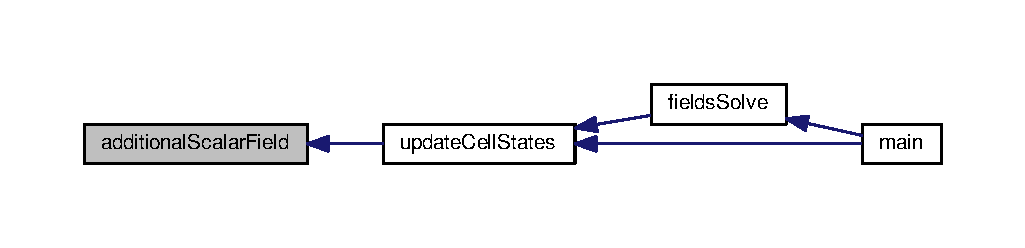
\includegraphics[width=350pt]{cells_8c_aa2ee543811c23ee4b487102bb71ba9c7_icgraph}
\end{center}
\end{figure}


\hypertarget{cells_8c_afdf0714d4b325131b21a0cbe42c44ece}{\index{cells.\-c@{cells.\-c}!cells\-Allocate@{cells\-Allocate}}
\index{cells\-Allocate@{cells\-Allocate}!cells.c@{cells.\-c}}
\subsubsection[{cells\-Allocate}]{\setlength{\rightskip}{0pt plus 5cm}void cells\-Allocate (
\begin{DoxyParamCaption}
{}
\end{DoxyParamCaption}
)}}\label{cells_8c_afdf0714d4b325131b21a0cbe42c44ece}
This function allocates tables responsible for carrying informations about cells, their current state and evolution. 

Definition at line 66 of file cells.\-c.



References cell\-Fields, cells, csize, local\-I\-D, max\-Cells, max\-Cells\-Per\-Proc, M\-P\-Isize, N\-F\-I\-E\-L\-D\-S, nx, sdim, stop\-Run(), tlnc, and velocity.


\begin{DoxyCode}
67 \{
68 
69   \textcolor{keywordtype}{int} i, j, c, f;
70   int64\_t cellsActualSize;
71 
72   \textcolor{keywordflow}{if} (\hyperlink{global_8h_a2f8118c1bfdf986827e156210c33cbab}{sdim} == 2)
73     \hyperlink{global_8h_a3b735e8520f1816ee73ee50daa3ef756}{csize} = (\hyperlink{global_8h_a02d47a4f36ec0bcce348696534567e30}{nx} / 2) / pow(8.0 * \hyperlink{global_8h_ac1a3e3adac8f1e6840fd332e3d3cfa21}{maxCells}, 1.0 / 2.0);
74   \textcolor{keywordflow}{if} (\hyperlink{global_8h_a2f8118c1bfdf986827e156210c33cbab}{sdim} == 3)
75     \hyperlink{global_8h_a3b735e8520f1816ee73ee50daa3ef756}{csize} = (\hyperlink{global_8h_a02d47a4f36ec0bcce348696534567e30}{nx} / 2) / pow(8.0 * \hyperlink{global_8h_ac1a3e3adac8f1e6840fd332e3d3cfa21}{maxCells}, 1.0 / 3.0);
76 
77   \hyperlink{global_8h_a2de426dd266cfdaaf6fb52ba3dc2740a}{maxCellsPerProc} = 1.5 * \hyperlink{global_8h_ac1a3e3adac8f1e6840fd332e3d3cfa21}{maxCells} / \hyperlink{global_8h_a0d7d02544d01ceac87c9d5cadc3af0df}{MPIsize};
78 
79   cellsActualSize = \hyperlink{global_8h_a2de426dd266cfdaaf6fb52ba3dc2740a}{maxCellsPerProc} * \textcolor{keyword}{sizeof}(\textcolor{keyword}{struct }\hyperlink{structcellData}{cellData});
80 
81   \hyperlink{global_8h_a265cb7ee626de517ecec0f0ac60833a7}{localID} = 0;
82 
83   \textcolor{keywordflow}{if} (!(\hyperlink{global_8h_a56da06a03aa369ca203be968cb56d16c}{cells} = (\textcolor{keyword}{struct} \hyperlink{structcellData}{cellData} *) malloc(cellsActualSize)))
84     \hyperlink{utils_8c_a07dd99a04f2723be164531a7a862fb67}{stopRun}(106, \textcolor{stringliteral}{"cells"}, \_\_FILE\_\_, \_\_LINE\_\_);
85 
86   \textcolor{keywordflow}{if} (!
87       (\hyperlink{global_8h_a6015afb23ea197551ff3d503aa3426a4}{velocity} =
88        (\textcolor{keyword}{struct} \hyperlink{structdoubleVector3d}{doubleVector3d} *) malloc(\hyperlink{global_8h_a2de426dd266cfdaaf6fb52ba3dc2740a}{maxCellsPerProc} *
89                     \textcolor{keyword}{sizeof}(\textcolor{keyword}{struct} \hyperlink{structdoubleVector3d}{doubleVector3d}))))
90     \hyperlink{utils_8c_a07dd99a04f2723be164531a7a862fb67}{stopRun}(106, \textcolor{stringliteral}{"velocity"}, \_\_FILE\_\_, \_\_LINE\_\_);
91 
92   \hyperlink{global_8h_a25e4317a1b5bb95a8e71e0e8c4e11f2b}{cellFields} = (\textcolor{keywordtype}{double} **) malloc(\hyperlink{fields_8h_a7986f01c038f396ce7df280bb2903099}{NFIELDS} * \textcolor{keyword}{sizeof}(\textcolor{keywordtype}{double} *));
93   \textcolor{keywordflow}{for} (f = 0; f < \hyperlink{fields_8h_a7986f01c038f396ce7df280bb2903099}{NFIELDS}; f++)
94     \textcolor{keywordflow}{if} (!
95     (\hyperlink{global_8h_a25e4317a1b5bb95a8e71e0e8c4e11f2b}{cellFields}[f] =
96      (\textcolor{keywordtype}{double} *) malloc(\hyperlink{global_8h_a2de426dd266cfdaaf6fb52ba3dc2740a}{maxCellsPerProc} * \textcolor{keyword}{sizeof}(\textcolor{keywordtype}{double}))))
97       \hyperlink{utils_8c_a07dd99a04f2723be164531a7a862fb67}{stopRun}(106, \textcolor{stringliteral}{"cellFields"}, \_\_FILE\_\_, \_\_LINE\_\_);
98 
99   \textcolor{keywordflow}{if} (!(\hyperlink{global_8h_ac3c96b975a3376c555ad22a7d2688b2f}{tlnc} = (int64\_t *) calloc(\hyperlink{global_8h_a0d7d02544d01ceac87c9d5cadc3af0df}{MPIsize}, \textcolor{keyword}{sizeof}(int64\_t))))
100     \hyperlink{utils_8c_a07dd99a04f2723be164531a7a862fb67}{stopRun}(106, \textcolor{stringliteral}{"tlnc"}, \_\_FILE\_\_, \_\_LINE\_\_);
101 
102 \}
\end{DoxyCode}


Here is the call graph for this function\-:\nopagebreak
\begin{figure}[H]
\begin{center}
\leavevmode
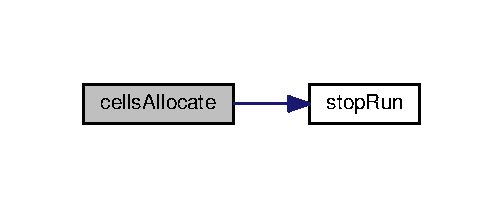
\includegraphics[width=242pt]{cells_8c_afdf0714d4b325131b21a0cbe42c44ece_cgraph}
\end{center}
\end{figure}




Here is the caller graph for this function\-:\nopagebreak
\begin{figure}[H]
\begin{center}
\leavevmode
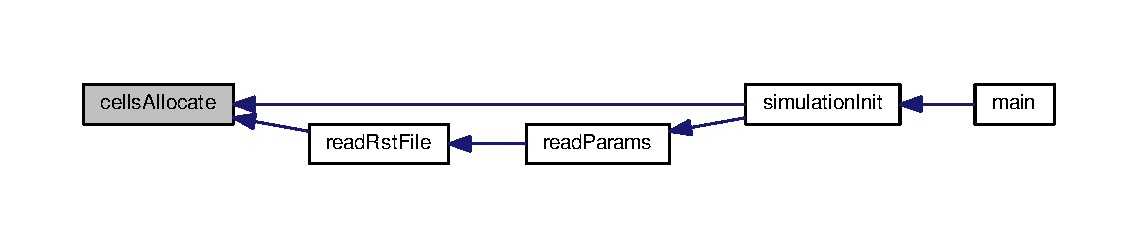
\includegraphics[width=350pt]{cells_8c_afdf0714d4b325131b21a0cbe42c44ece_icgraph}
\end{center}
\end{figure}


\hypertarget{cells_8c_aead37c061c3f1ec47259afaf2783029f}{\index{cells.\-c@{cells.\-c}!cells\-Cleanup@{cells\-Cleanup}}
\index{cells\-Cleanup@{cells\-Cleanup}!cells.c@{cells.\-c}}
\subsubsection[{cells\-Cleanup}]{\setlength{\rightskip}{0pt plus 5cm}void cells\-Cleanup (
\begin{DoxyParamCaption}
{}
\end{DoxyParamCaption}
)}}\label{cells_8c_aead37c061c3f1ec47259afaf2783029f}
This function dealocates all tables allocated during initialization of cell data 

Definition at line 434 of file cells.\-c.



References cell\-Fields, cells, N\-F\-I\-E\-L\-D\-S, tlnc, and velocity.


\begin{DoxyCode}
435 \{
436   \textcolor{keywordtype}{int} f;
437   free(\hyperlink{global_8h_ac3c96b975a3376c555ad22a7d2688b2f}{tlnc});
438   free(\hyperlink{global_8h_a56da06a03aa369ca203be968cb56d16c}{cells});
439   \textcolor{keywordflow}{for} (f = 0; f < \hyperlink{fields_8h_a7986f01c038f396ce7df280bb2903099}{NFIELDS}; f++)
440     free(\hyperlink{global_8h_a25e4317a1b5bb95a8e71e0e8c4e11f2b}{cellFields}[f]);
441   free(\hyperlink{global_8h_a25e4317a1b5bb95a8e71e0e8c4e11f2b}{cellFields});
442   free(\hyperlink{global_8h_a6015afb23ea197551ff3d503aa3426a4}{velocity});
443 \}
\end{DoxyCode}


Here is the caller graph for this function\-:\nopagebreak
\begin{figure}[H]
\begin{center}
\leavevmode
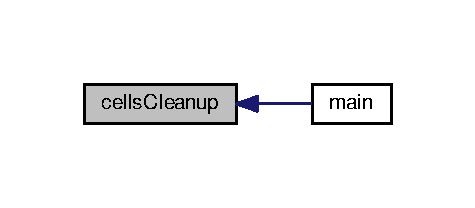
\includegraphics[width=228pt]{cells_8c_aead37c061c3f1ec47259afaf2783029f_icgraph}
\end{center}
\end{figure}


\hypertarget{cells_8c_aa2527c8374034b85c4e95b665786b0ca}{\index{cells.\-c@{cells.\-c}!cells\-Cycle\-Init@{cells\-Cycle\-Init}}
\index{cells\-Cycle\-Init@{cells\-Cycle\-Init}!cells.c@{cells.\-c}}
\subsubsection[{cells\-Cycle\-Init}]{\setlength{\rightskip}{0pt plus 5cm}void cells\-Cycle\-Init (
\begin{DoxyParamCaption}
{}
\end{DoxyParamCaption}
)}}\label{cells_8c_aa2527c8374034b85c4e95b665786b0ca}
This function initializes counters of cells in various cell phases. 

Definition at line 107 of file cells.\-c.



References cancer, cnc, g0nc, g1nc, g2nc, lcnc, lg0nc, lg1nc, lg2nc, lmnc, lnc, lnnc, lsnc, mnc, nc, and snc.


\begin{DoxyCode}
108 \{
109   \textcolor{comment}{/* global numbers of cells */}
110   \hyperlink{global_8h_a33c78f8734fc6805cec2755dd09e0117}{g0nc} = \hyperlink{global_8h_a0845b4b004824f1fe3cd69db1672fa15}{nc};
111   \hyperlink{global_8h_a09b30abbc9cc684e55a246df0528a14b}{g1nc} = 0;
112   \hyperlink{global_8h_a0e24070582e0ecd757fdbdee28c8ff4e}{snc} = 0;
113   \hyperlink{global_8h_ae6288fa86281103b55c317d7f88dca28}{g2nc} = 0;
114   \hyperlink{global_8h_ad1cd19943c182708694e74186fb08015}{mnc} = 0;
115   \hyperlink{global_8h_aec5760e92b3bdf9ac05fc2920446ecd8}{cnc} = 0;
116   \textcolor{comment}{/* local numbers of cells */}
117   \hyperlink{global_8h_a356af225353f2a5512be222c1354bee3}{lg0nc} = \hyperlink{global_8h_a7065c019590815f10169c219f358e7d0}{lnc};
118   \hyperlink{global_8h_a59dc7e07b6be86e29bd0e9f3f18c3ca2}{lg1nc} = 0;
119   \hyperlink{global_8h_af5e326c959f5815222d8f8e3f4d66419}{lsnc} = 0;
120   \hyperlink{global_8h_a17ca9380dca478aa01c68ce4cc8ca720}{lg2nc} = 0;
121   \hyperlink{global_8h_a002cff2ccc4cfc5b5f85ac5ea285ef9c}{lmnc} = 0;
122   \hyperlink{global_8h_ab67f763fa0f30ce2912a6ab60dc8e648}{lcnc} = 0;
123   \hyperlink{global_8h_a97370c479716d79f799616103c487d51}{lnnc} = 0;
124   \textcolor{comment}{/* number of cancer cells */}
125   \hyperlink{global_8h_a543a1902d49aca54ef382bf603a51e27}{cancer} = 0;
126 \}
\end{DoxyCode}


Here is the caller graph for this function\-:\nopagebreak
\begin{figure}[H]
\begin{center}
\leavevmode
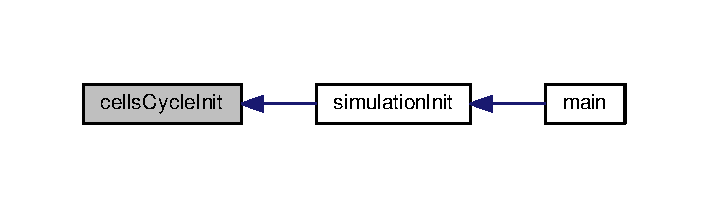
\includegraphics[width=340pt]{cells_8c_aa2527c8374034b85c4e95b665786b0ca_icgraph}
\end{center}
\end{figure}


\hypertarget{cells_8c_a8101c456dae07ab9cbd918ccad3a2ff7}{\index{cells.\-c@{cells.\-c}!cells\-Death@{cells\-Death}}
\index{cells\-Death@{cells\-Death}!cells.c@{cells.\-c}}
\subsubsection[{cells\-Death}]{\setlength{\rightskip}{0pt plus 5cm}void cells\-Death (
\begin{DoxyParamCaption}
\item[{int}]{lnc\-\_\-old}
\end{DoxyParamCaption}
)}}\label{cells_8c_a8101c456dae07ab9cbd918ccad3a2ff7}
This function removes a dead cell from the simulation. 

Definition at line 448 of file cells.\-c.



References celld, cells, lcnc, lg0nc, lg1nc, lg2nc, lmnc, lnc, lsnc, and rsum.


\begin{DoxyCode}
449 \{
450   \textcolor{keywordtype}{int} c, pos;
451 
452   pos = 0;
453   \textcolor{keywordflow}{for} (c = 0; c < \hyperlink{global_8h_a7065c019590815f10169c219f358e7d0}{lnc}; c++) \{
454     \textcolor{comment}{/* shift cells after dead cell removal */}
455     \textcolor{keywordflow}{if} (c >= lnc\_old) \{
456       \hyperlink{global_8h_a56da06a03aa369ca203be968cb56d16c}{cells}[pos] = \hyperlink{global_8h_a56da06a03aa369ca203be968cb56d16c}{cells}[c];
457       pos++;
458       \textcolor{keywordflow}{continue};
459     \}
460     \textcolor{keywordflow}{if} (c != pos && \hyperlink{cells_8c_a96a825c021fe648b7fb171bd2c532ffb}{celld}[c] == 0)
461       \hyperlink{global_8h_a56da06a03aa369ca203be968cb56d16c}{cells}[pos] = \hyperlink{global_8h_a56da06a03aa369ca203be968cb56d16c}{cells}[c];
462     \textcolor{keywordflow}{if} (\hyperlink{cells_8c_a96a825c021fe648b7fb171bd2c532ffb}{celld}[c] == 0)
463       pos++;
464     \textcolor{comment}{/* update cell counters */}
465     \textcolor{keywordflow}{if} (\hyperlink{cells_8c_a96a825c021fe648b7fb171bd2c532ffb}{celld}[c] == 1) \{
466       \textcolor{keywordflow}{switch} (\hyperlink{global_8h_a56da06a03aa369ca203be968cb56d16c}{cells}[c].\hyperlink{structcellData_accf3aec63bc20b3c99ab4881cb07c05b}{phase}) \{
467       \textcolor{keywordflow}{case} 0:
468     \hyperlink{global_8h_a356af225353f2a5512be222c1354bee3}{lg0nc}--;
469     \textcolor{keywordflow}{break};
470       \textcolor{keywordflow}{case} 1:
471     \hyperlink{global_8h_a59dc7e07b6be86e29bd0e9f3f18c3ca2}{lg1nc}--;
472     \textcolor{keywordflow}{break};
473       \textcolor{keywordflow}{case} 2:
474     \hyperlink{global_8h_af5e326c959f5815222d8f8e3f4d66419}{lsnc}--;
475     \textcolor{keywordflow}{break};
476       \textcolor{keywordflow}{case} 3:
477     \hyperlink{global_8h_a17ca9380dca478aa01c68ce4cc8ca720}{lg2nc}--;
478     \textcolor{keywordflow}{break};
479       \textcolor{keywordflow}{case} 4:
480     \hyperlink{global_8h_a002cff2ccc4cfc5b5f85ac5ea285ef9c}{lmnc}--;
481     \textcolor{keywordflow}{break};
482       \}
483       \textcolor{keywordflow}{if} (\hyperlink{global_8h_a56da06a03aa369ca203be968cb56d16c}{cells}[c].\hyperlink{structcellData_a49af8c5336d6c2401bc24f86dbb97b36}{tumor} == 1)
484     \hyperlink{global_8h_ab67f763fa0f30ce2912a6ab60dc8e648}{lcnc}--;
485     \}
486   \}
487   lnc -= \hyperlink{global_8h_a087a95bb36c9b36c708a73ce656fd1f1}{rsum};
488 \}
\end{DoxyCode}


Here is the caller graph for this function\-:\nopagebreak
\begin{figure}[H]
\begin{center}
\leavevmode
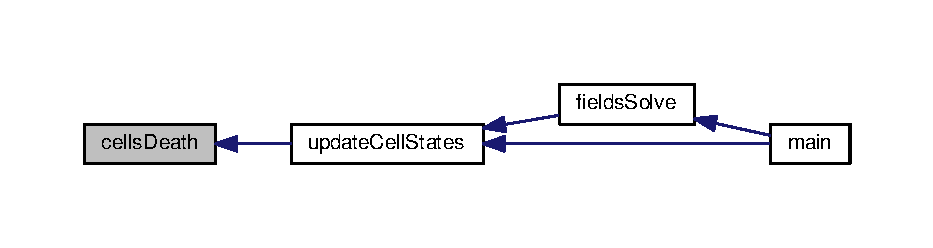
\includegraphics[width=350pt]{cells_8c_a8101c456dae07ab9cbd918ccad3a2ff7_icgraph}
\end{center}
\end{figure}


\hypertarget{cells_8c_a68e70197591e819d22315879c8141bdd}{\index{cells.\-c@{cells.\-c}!cells\-Random\-Init@{cells\-Random\-Init}}
\index{cells\-Random\-Init@{cells\-Random\-Init}!cells.c@{cells.\-c}}
\subsubsection[{cells\-Random\-Init}]{\setlength{\rightskip}{0pt plus 5cm}int cells\-Random\-Init (
\begin{DoxyParamCaption}
{}
\end{DoxyParamCaption}
)}}\label{cells_8c_a68e70197591e819d22315879c8141bdd}
This function initializes cell data. Locations of cells in space are generated randomly. 

Definition at line 132 of file cells.\-c.



References cell\-Data\-::age, cells, csize, cell\-Data\-::death, cell\-Data\-::density, cell\-Data\-::g1, g1, cell\-Data\-::g2, g2, cell\-Data\-::gid, cell\-Data\-::h, h, h2, h3, h4, cell\-Data\-::halo, lnc, local\-I\-D, cell\-Data\-::m, m, max\-Cells, max\-Cells\-Per\-Proc, M\-P\-Irank, nc, nx, cell\-Data\-::phase, cell\-Data\-::phasetime, rng, cell\-Data\-::s, s, sdim, sim\-Time, cell\-Data\-::size, stream, cell\-Data\-::tumor, cell\-Data\-::v, v, cell\-Data\-::x, cell\-Data\-::y, cell\-Data\-::young, and cell\-Data\-::z.


\begin{DoxyCode}
133 \{
134 
135   \textcolor{keywordtype}{int} i, j;
136 
137   \textcolor{comment}{/* uniform distribution */}
138   \textcolor{keywordflow}{if} (!strcmp(\hyperlink{global_8h_ae94cd2e37eb46a6942cc45e1b29f87fc}{rng}, \textcolor{stringliteral}{"UNB"})) \{
139     \textcolor{keywordtype}{double} D;
140 
141     \textcolor{keywordflow}{if} (\hyperlink{global_8h_a2f8118c1bfdf986827e156210c33cbab}{sdim} == 2)
142       \hyperlink{global_8h_a3b735e8520f1816ee73ee50daa3ef756}{csize} = (\hyperlink{global_8h_a02d47a4f36ec0bcce348696534567e30}{nx} / 2) / pow(8.0 * \hyperlink{global_8h_ac1a3e3adac8f1e6840fd332e3d3cfa21}{maxCells}, 1.0 / 2.0);
143     \textcolor{keywordflow}{if} (\hyperlink{global_8h_a2f8118c1bfdf986827e156210c33cbab}{sdim} == 3)
144       \hyperlink{global_8h_a3b735e8520f1816ee73ee50daa3ef756}{csize} = (\hyperlink{global_8h_a02d47a4f36ec0bcce348696534567e30}{nx} / 2) / pow(8.0 * \hyperlink{global_8h_ac1a3e3adac8f1e6840fd332e3d3cfa21}{maxCells}, 1.0 / 3.0);
145     \textcolor{keywordflow}{if} (\hyperlink{global_8h_a2f8118c1bfdf986827e156210c33cbab}{sdim} == 2)
146       D = \hyperlink{global_8h_a3b735e8520f1816ee73ee50daa3ef756}{csize} * pow(8.0 * \hyperlink{global_8h_a0845b4b004824f1fe3cd69db1672fa15}{nc}, 1.0 / 2.0);
147     \textcolor{keywordflow}{if} (\hyperlink{global_8h_a2f8118c1bfdf986827e156210c33cbab}{sdim} == 3)
148       D = \hyperlink{global_8h_a3b735e8520f1816ee73ee50daa3ef756}{csize} * pow(8.0 * \hyperlink{global_8h_a0845b4b004824f1fe3cd69db1672fa15}{nc}, 1.0 / 3.0);
149 
150     \hyperlink{global_8h_a8ee9be1b5aa75abae556de3088cba6d9}{h} = 3.0 * \hyperlink{global_8h_a3b735e8520f1816ee73ee50daa3ef756}{csize};
151     \hyperlink{global_8h_ad188f0f25b4773be09b6eb6babe59f59}{simTime} = 0;
152 
153     \textcolor{keywordflow}{for} (i = 0; i < \hyperlink{global_8h_a7065c019590815f10169c219f358e7d0}{lnc}; i++) \{
154       \hyperlink{global_8h_a56da06a03aa369ca203be968cb56d16c}{cells}[i].\hyperlink{structcellData_af88b946fb90d5f08b5fb740c70e98c10}{x} = D * (sprng(\hyperlink{global_8h_a5340130b6fb2647cef6b71354e27b0d4}{stream}) * 2 - 1);
155       \hyperlink{global_8h_a56da06a03aa369ca203be968cb56d16c}{cells}[i].\hyperlink{structcellData_ab927965981178aa1fba979a37168db2a}{y} = D * (sprng(\hyperlink{global_8h_a5340130b6fb2647cef6b71354e27b0d4}{stream}) * 2 - 1);
156       \textcolor{keywordflow}{if} (\hyperlink{global_8h_a2f8118c1bfdf986827e156210c33cbab}{sdim} == 3)
157     \hyperlink{global_8h_a56da06a03aa369ca203be968cb56d16c}{cells}[i].\hyperlink{structcellData_ab3e6ed577a7c669c19de1f9c1b46c872}{z} = D * (sprng(\hyperlink{global_8h_a5340130b6fb2647cef6b71354e27b0d4}{stream}) * 2 - 1);
158       \textcolor{keywordflow}{else}
159     \hyperlink{global_8h_a56da06a03aa369ca203be968cb56d16c}{cells}[i].\hyperlink{structcellData_ab3e6ed577a7c669c19de1f9c1b46c872}{z} = 0.0;
160 
161       \hyperlink{global_8h_a56da06a03aa369ca203be968cb56d16c}{cells}[i].\hyperlink{structcellData_af88b946fb90d5f08b5fb740c70e98c10}{x} += \hyperlink{global_8h_a02d47a4f36ec0bcce348696534567e30}{nx} / 2;
162       \hyperlink{global_8h_a56da06a03aa369ca203be968cb56d16c}{cells}[i].\hyperlink{structcellData_ab927965981178aa1fba979a37168db2a}{y} += \hyperlink{global_8h_a02d47a4f36ec0bcce348696534567e30}{nx} / 2;
163       \textcolor{keywordflow}{if} (\hyperlink{global_8h_a2f8118c1bfdf986827e156210c33cbab}{sdim} == 3)
164     \hyperlink{global_8h_a56da06a03aa369ca203be968cb56d16c}{cells}[i].\hyperlink{structcellData_ab3e6ed577a7c669c19de1f9c1b46c872}{z} += \hyperlink{global_8h_a02d47a4f36ec0bcce348696534567e30}{nx} / 2;
165       \textcolor{keywordflow}{else}
166     \hyperlink{global_8h_a56da06a03aa369ca203be968cb56d16c}{cells}[i].\hyperlink{structcellData_ab3e6ed577a7c669c19de1f9c1b46c872}{z} = 0.0;
167 
168       \hyperlink{global_8h_a56da06a03aa369ca203be968cb56d16c}{cells}[i].\hyperlink{structcellData_aba3c5d750d5dbd6e86c11ecaca62885e}{size} = pow(2.0, -(1.0 / 3.0)) * \hyperlink{global_8h_a3b735e8520f1816ee73ee50daa3ef756}{csize};
169       \hyperlink{global_8h_a56da06a03aa369ca203be968cb56d16c}{cells}[i].\hyperlink{structcellData_abb4d4bd9231e9f994e87f32cc4fcfce8}{gid} =
170       (\textcolor{keywordtype}{unsigned} \textcolor{keywordtype}{long} \textcolor{keywordtype}{long} int) \hyperlink{global_8h_a710288ab7d2734acc4566a87a645325d}{MPIrank} *(\textcolor{keywordtype}{unsigned} \textcolor{keywordtype}{long} \textcolor{keywordtype}{long} \textcolor{keywordtype}{int})
171       \hyperlink{global_8h_a2de426dd266cfdaaf6fb52ba3dc2740a}{maxCellsPerProc} + (\textcolor{keywordtype}{unsigned} \textcolor{keywordtype}{long} \textcolor{keywordtype}{long} int) i;
172       \hyperlink{global_8h_a56da06a03aa369ca203be968cb56d16c}{cells}[i].\hyperlink{structcellData_a3b90d5a73541ab9402511d87bed076ef}{v} = 0.0;
173       \hyperlink{global_8h_a56da06a03aa369ca203be968cb56d16c}{cells}[i].\hyperlink{structcellData_a6f8c052f8417728038991f7f2826d38d}{density} = 0.0;
174       \hyperlink{global_8h_a56da06a03aa369ca203be968cb56d16c}{cells}[i].\hyperlink{structcellData_a8ee9be1b5aa75abae556de3088cba6d9}{h} = \hyperlink{global_8h_a8ee9be1b5aa75abae556de3088cba6d9}{h};
175       \hyperlink{global_8h_a56da06a03aa369ca203be968cb56d16c}{cells}[i].\hyperlink{structcellData_ad0bd87a264e65d1c17ecc07049819f2c}{young} = 2100.0 + sprng(\hyperlink{global_8h_a5340130b6fb2647cef6b71354e27b0d4}{stream}) * 100.0;
176       \hyperlink{global_8h_a56da06a03aa369ca203be968cb56d16c}{cells}[i].\hyperlink{structcellData_a80ff3fcc4d03d0b1b01559839d12df5b}{halo} = 0;
177       \hyperlink{global_8h_a56da06a03aa369ca203be968cb56d16c}{cells}[i].\hyperlink{structcellData_accf3aec63bc20b3c99ab4881cb07c05b}{phase} = 0;
178       \hyperlink{global_8h_a56da06a03aa369ca203be968cb56d16c}{cells}[i].\hyperlink{structcellData_a581debe7d16bce9d187b97855f4e99d4}{g1} = \hyperlink{global_8h_a581debe7d16bce9d187b97855f4e99d4}{g1} * (1 + (sprng(\hyperlink{global_8h_a5340130b6fb2647cef6b71354e27b0d4}{stream}) * 2 - 1) * \hyperlink{global_8h_a48d9522e58fa05906c6dba23e5745a72}{v});
179       \hyperlink{global_8h_a56da06a03aa369ca203be968cb56d16c}{cells}[i].\hyperlink{structcellData_aee9971139118d56815564304450c4775}{g2} = \hyperlink{global_8h_aee9971139118d56815564304450c4775}{g2} * (1 + (sprng(\hyperlink{global_8h_a5340130b6fb2647cef6b71354e27b0d4}{stream}) * 2 - 1) * \hyperlink{global_8h_a48d9522e58fa05906c6dba23e5745a72}{v});
180       \hyperlink{global_8h_a56da06a03aa369ca203be968cb56d16c}{cells}[i].\hyperlink{structcellData_a874f74a4dc1c9a0cd9c6e0d79c298f55}{s} = \hyperlink{global_8h_a874f74a4dc1c9a0cd9c6e0d79c298f55}{s} * (1 + (sprng(\hyperlink{global_8h_a5340130b6fb2647cef6b71354e27b0d4}{stream}) * 2 - 1) * \hyperlink{global_8h_a48d9522e58fa05906c6dba23e5745a72}{v});
181       \hyperlink{global_8h_a56da06a03aa369ca203be968cb56d16c}{cells}[i].\hyperlink{structcellData_ac51334f57ef8b81c0629c9421798c344}{m} = \hyperlink{global_8h_ac51334f57ef8b81c0629c9421798c344}{m} * (1 + (sprng(\hyperlink{global_8h_a5340130b6fb2647cef6b71354e27b0d4}{stream}) * 2 - 1) * \hyperlink{global_8h_a48d9522e58fa05906c6dba23e5745a72}{v});
182       \hyperlink{global_8h_a56da06a03aa369ca203be968cb56d16c}{cells}[i].\hyperlink{structcellData_afe1297f954440c453b59fcb06992dbd5}{phasetime} = 0.0;
183       \hyperlink{global_8h_a56da06a03aa369ca203be968cb56d16c}{cells}[i].\hyperlink{structcellData_a91d98a856bbd96810b40af3ca5cc901a}{age} = 0;
184       \hyperlink{global_8h_a56da06a03aa369ca203be968cb56d16c}{cells}[i].\hyperlink{structcellData_add1e1533be6e693ffedcdbafdf8b855c}{death} = 0;
185       \hyperlink{global_8h_a56da06a03aa369ca203be968cb56d16c}{cells}[i].\hyperlink{structcellData_a49af8c5336d6c2401bc24f86dbb97b36}{tumor} = 0;
186       \hyperlink{global_8h_a265cb7ee626de517ecec0f0ac60833a7}{localID}++;
187     \}
188   \}
189   \textcolor{comment}{/* normal distribution (Box-Muller transform) */}
190   \textcolor{keywordflow}{if} (!strcmp(\hyperlink{global_8h_ae94cd2e37eb46a6942cc45e1b29f87fc}{rng}, \textcolor{stringliteral}{"BM"})) \{
191     \textcolor{keywordtype}{double} x1, x2, x3;
192     \textcolor{keywordtype}{double} z1, z2, z3;
193     \textcolor{keywordtype}{double} r1, r2;
194     \textcolor{keywordtype}{double} l;
195     \textcolor{keywordtype}{double} D;
196     \textcolor{keywordflow}{if} (\hyperlink{global_8h_a2f8118c1bfdf986827e156210c33cbab}{sdim} == 2)
197       \hyperlink{global_8h_a3b735e8520f1816ee73ee50daa3ef756}{csize} = (\hyperlink{global_8h_a02d47a4f36ec0bcce348696534567e30}{nx} / 2) / pow(8.0 * \hyperlink{global_8h_ac1a3e3adac8f1e6840fd332e3d3cfa21}{maxCells}, 1.0 / 2.0);
198     \textcolor{keywordflow}{if} (\hyperlink{global_8h_a2f8118c1bfdf986827e156210c33cbab}{sdim} == 3)
199       \hyperlink{global_8h_a3b735e8520f1816ee73ee50daa3ef756}{csize} = (\hyperlink{global_8h_a02d47a4f36ec0bcce348696534567e30}{nx} / 2) / pow(8.0 * \hyperlink{global_8h_ac1a3e3adac8f1e6840fd332e3d3cfa21}{maxCells}, 1.0 / 3.0);
200     \textcolor{keywordflow}{if} (\hyperlink{global_8h_a2f8118c1bfdf986827e156210c33cbab}{sdim} == 2)
201       D = \hyperlink{global_8h_a3b735e8520f1816ee73ee50daa3ef756}{csize} * pow(8.0 * \hyperlink{global_8h_a0845b4b004824f1fe3cd69db1672fa15}{nc}, 1.0 / 2.0);
202     \textcolor{keywordflow}{if} (\hyperlink{global_8h_a2f8118c1bfdf986827e156210c33cbab}{sdim} == 3)
203       D = \hyperlink{global_8h_a3b735e8520f1816ee73ee50daa3ef756}{csize} * pow(8.0 * \hyperlink{global_8h_a0845b4b004824f1fe3cd69db1672fa15}{nc}, 1.0 / 3.0);
204 
205     \hyperlink{global_8h_a8ee9be1b5aa75abae556de3088cba6d9}{h} = 3.0 * \hyperlink{global_8h_a3b735e8520f1816ee73ee50daa3ef756}{csize};
206     \hyperlink{global_8h_ad188f0f25b4773be09b6eb6babe59f59}{simTime} = 0;
207 
208     \textcolor{keywordflow}{for} (i = 0; i < \hyperlink{global_8h_a7065c019590815f10169c219f358e7d0}{lnc}; i++) \{
209 
210       r2 = 1.1;
211 
212       \textcolor{keywordflow}{while} (r2 >= 1.0) \{
213     r1 = 1.1;
214     \textcolor{keywordflow}{while} (r1 == 0 || r1 >= 1.0) \{
215       x1 = sprng(\hyperlink{global_8h_a5340130b6fb2647cef6b71354e27b0d4}{stream}) * 2 - 1;
216       x2 = sprng(\hyperlink{global_8h_a5340130b6fb2647cef6b71354e27b0d4}{stream}) * 2 - 1;
217       x3 = sprng(\hyperlink{global_8h_a5340130b6fb2647cef6b71354e27b0d4}{stream}) * 2 - 1;
218       r1 = x1 * x1 + x2 * x2 + x3 * x3;
219     \}
220     l = sqrt(-2 * log(r1) / r1);
221     z1 = x1 * l;
222     z2 = x2 * l;
223     z3 = x3 * l;
224 
225     r2 = z1 * z1 + z2 * z2 + z3 * z3;
226       \}
227 
228       \hyperlink{global_8h_a56da06a03aa369ca203be968cb56d16c}{cells}[i].\hyperlink{structcellData_af88b946fb90d5f08b5fb740c70e98c10}{x} = z1 * D + \hyperlink{global_8h_a02d47a4f36ec0bcce348696534567e30}{nx} / 2;
229       \hyperlink{global_8h_a56da06a03aa369ca203be968cb56d16c}{cells}[i].\hyperlink{structcellData_ab927965981178aa1fba979a37168db2a}{y} = z2 * D + \hyperlink{global_8h_a02d47a4f36ec0bcce348696534567e30}{nx} / 2;
230       \textcolor{keywordflow}{if} (\hyperlink{global_8h_a2f8118c1bfdf986827e156210c33cbab}{sdim} == 3)
231     \hyperlink{global_8h_a56da06a03aa369ca203be968cb56d16c}{cells}[i].\hyperlink{structcellData_ab3e6ed577a7c669c19de1f9c1b46c872}{z} = z3 * D + \hyperlink{global_8h_a02d47a4f36ec0bcce348696534567e30}{nx} / 2;
232       \textcolor{keywordflow}{else}
233     \hyperlink{global_8h_a56da06a03aa369ca203be968cb56d16c}{cells}[i].\hyperlink{structcellData_ab3e6ed577a7c669c19de1f9c1b46c872}{z} = 0.0;
234 
235       \hyperlink{global_8h_a56da06a03aa369ca203be968cb56d16c}{cells}[i].\hyperlink{structcellData_aba3c5d750d5dbd6e86c11ecaca62885e}{size} = pow(2.0, -(1.0 / 3.0)) * \hyperlink{global_8h_a3b735e8520f1816ee73ee50daa3ef756}{csize};
236       \hyperlink{global_8h_a56da06a03aa369ca203be968cb56d16c}{cells}[i].\hyperlink{structcellData_abb4d4bd9231e9f994e87f32cc4fcfce8}{gid} =
237       (\textcolor{keywordtype}{unsigned} \textcolor{keywordtype}{long} \textcolor{keywordtype}{long} int) \hyperlink{global_8h_a710288ab7d2734acc4566a87a645325d}{MPIrank} *(\textcolor{keywordtype}{unsigned} \textcolor{keywordtype}{long} \textcolor{keywordtype}{long} \textcolor{keywordtype}{int})
238       \hyperlink{global_8h_a2de426dd266cfdaaf6fb52ba3dc2740a}{maxCellsPerProc} + (\textcolor{keywordtype}{unsigned} \textcolor{keywordtype}{long} \textcolor{keywordtype}{long} int) i;
239       \hyperlink{global_8h_a56da06a03aa369ca203be968cb56d16c}{cells}[i].\hyperlink{structcellData_a3b90d5a73541ab9402511d87bed076ef}{v} = 0.0;
240       \hyperlink{global_8h_a56da06a03aa369ca203be968cb56d16c}{cells}[i].\hyperlink{structcellData_a6f8c052f8417728038991f7f2826d38d}{density} = 0.0;
241       \hyperlink{global_8h_a56da06a03aa369ca203be968cb56d16c}{cells}[i].\hyperlink{structcellData_a8ee9be1b5aa75abae556de3088cba6d9}{h} = \hyperlink{global_8h_a8ee9be1b5aa75abae556de3088cba6d9}{h};
242       \hyperlink{global_8h_a56da06a03aa369ca203be968cb56d16c}{cells}[i].\hyperlink{structcellData_ad0bd87a264e65d1c17ecc07049819f2c}{young} = 2100.0 + sprng(\hyperlink{global_8h_a5340130b6fb2647cef6b71354e27b0d4}{stream}) * 100.0;
243       \hyperlink{global_8h_a56da06a03aa369ca203be968cb56d16c}{cells}[i].\hyperlink{structcellData_a80ff3fcc4d03d0b1b01559839d12df5b}{halo} = 0;
244       \hyperlink{global_8h_a56da06a03aa369ca203be968cb56d16c}{cells}[i].\hyperlink{structcellData_accf3aec63bc20b3c99ab4881cb07c05b}{phase} = 0;
245       \hyperlink{global_8h_a56da06a03aa369ca203be968cb56d16c}{cells}[i].\hyperlink{structcellData_a581debe7d16bce9d187b97855f4e99d4}{g1} = \hyperlink{global_8h_a581debe7d16bce9d187b97855f4e99d4}{g1} * (1 + (sprng(\hyperlink{global_8h_a5340130b6fb2647cef6b71354e27b0d4}{stream}) * 2 - 1) * \hyperlink{global_8h_a48d9522e58fa05906c6dba23e5745a72}{v});
246       \hyperlink{global_8h_a56da06a03aa369ca203be968cb56d16c}{cells}[i].\hyperlink{structcellData_aee9971139118d56815564304450c4775}{g2} = \hyperlink{global_8h_aee9971139118d56815564304450c4775}{g2} * (1 + (sprng(\hyperlink{global_8h_a5340130b6fb2647cef6b71354e27b0d4}{stream}) * 2 - 1) * \hyperlink{global_8h_a48d9522e58fa05906c6dba23e5745a72}{v});
247       \hyperlink{global_8h_a56da06a03aa369ca203be968cb56d16c}{cells}[i].\hyperlink{structcellData_a874f74a4dc1c9a0cd9c6e0d79c298f55}{s} = \hyperlink{global_8h_a874f74a4dc1c9a0cd9c6e0d79c298f55}{s} * (1 + (sprng(\hyperlink{global_8h_a5340130b6fb2647cef6b71354e27b0d4}{stream}) * 2 - 1) * \hyperlink{global_8h_a48d9522e58fa05906c6dba23e5745a72}{v});
248       \hyperlink{global_8h_a56da06a03aa369ca203be968cb56d16c}{cells}[i].\hyperlink{structcellData_ac51334f57ef8b81c0629c9421798c344}{m} = \hyperlink{global_8h_ac51334f57ef8b81c0629c9421798c344}{m} * (1 + (sprng(\hyperlink{global_8h_a5340130b6fb2647cef6b71354e27b0d4}{stream}) * 2 - 1) * \hyperlink{global_8h_a48d9522e58fa05906c6dba23e5745a72}{v});
249       \hyperlink{global_8h_a56da06a03aa369ca203be968cb56d16c}{cells}[i].\hyperlink{structcellData_afe1297f954440c453b59fcb06992dbd5}{phasetime} = 0.0;
250       \hyperlink{global_8h_a56da06a03aa369ca203be968cb56d16c}{cells}[i].\hyperlink{structcellData_a49af8c5336d6c2401bc24f86dbb97b36}{tumor} = 0;
251       \hyperlink{global_8h_a56da06a03aa369ca203be968cb56d16c}{cells}[i].\hyperlink{structcellData_a91d98a856bbd96810b40af3ca5cc901a}{age} = 0;
252       \hyperlink{global_8h_a56da06a03aa369ca203be968cb56d16c}{cells}[i].\hyperlink{structcellData_add1e1533be6e693ffedcdbafdf8b855c}{death} = 0;
253       \hyperlink{global_8h_a265cb7ee626de517ecec0f0ac60833a7}{localID}++;
254     \}
255   \}
256 
257   \textcolor{comment}{/* powers of h are calculated only once here */}
258   \hyperlink{global_8h_ac2d9b75feeec68992c955b63e813e7ce}{h2} = \hyperlink{global_8h_a8ee9be1b5aa75abae556de3088cba6d9}{h} * \hyperlink{global_8h_a8ee9be1b5aa75abae556de3088cba6d9}{h};
259   \hyperlink{global_8h_adafe1d7389480b1a329b70b3c2baed11}{h3} = \hyperlink{global_8h_ac2d9b75feeec68992c955b63e813e7ce}{h2} * \hyperlink{global_8h_a8ee9be1b5aa75abae556de3088cba6d9}{h};
260   \hyperlink{global_8h_a40b544b5f22197434cf4bb2ccca5c8a6}{h4} = \hyperlink{global_8h_adafe1d7389480b1a329b70b3c2baed11}{h3} * \hyperlink{global_8h_a8ee9be1b5aa75abae556de3088cba6d9}{h};
261 \}
\end{DoxyCode}


Here is the caller graph for this function\-:\nopagebreak
\begin{figure}[H]
\begin{center}
\leavevmode
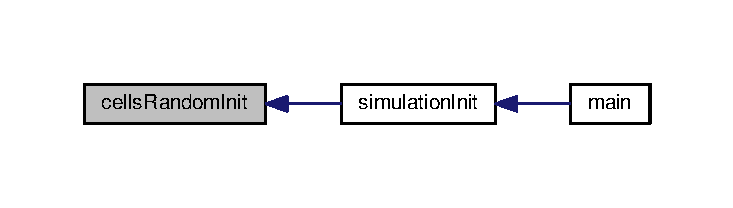
\includegraphics[width=350pt]{cells_8c_a68e70197591e819d22315879c8141bdd_icgraph}
\end{center}
\end{figure}


\hypertarget{cells_8c_a00dbe1f9f23fc7385462c32b89d28cf8}{\index{cells.\-c@{cells.\-c}!mark\-Middle\-Cancer\-Cell@{mark\-Middle\-Cancer\-Cell}}
\index{mark\-Middle\-Cancer\-Cell@{mark\-Middle\-Cancer\-Cell}!cells.c@{cells.\-c}}
\subsubsection[{mark\-Middle\-Cancer\-Cell}]{\setlength{\rightskip}{0pt plus 5cm}void mark\-Middle\-Cancer\-Cell (
\begin{DoxyParamCaption}
{}
\end{DoxyParamCaption}
)}}\label{cells_8c_a00dbe1f9f23fc7385462c32b89d28cf8}
This function finds locates cell closest to the center of mass of the system and marks this cell as a cancer cell. 

Definition at line 374 of file cells.\-c.



References cancer, cells, lcnc, lg0nc, lg1nc, lnc, M\-P\-Irank, nc, cell\-Data\-::phase, cell\-Data\-::tumor, x, cell\-Data\-::x, cell\-Data\-::y, and cell\-Data\-::z.


\begin{DoxyCode}
375 \{
376   \textcolor{keywordtype}{int} c;
377   \textcolor{keywordtype}{int} middle = 0;
378   \textcolor{keywordtype}{double} dist;
379   \textcolor{keyword}{struct }\{
380     \textcolor{keywordtype}{double} val;
381     \textcolor{keywordtype}{int} rank;
382   \} lmdist, gmdist;
383   \textcolor{keywordtype}{double} center[3];
384   \textcolor{keywordtype}{double} gcenter[3];
385 
386   \textcolor{comment}{/* each process computes its local center of mass */}
387   center[0] = 0.0;
388   center[1] = 0.0;
389   center[2] = 0.0;
390   \textcolor{keywordflow}{for} (c = 0; c < \hyperlink{global_8h_a7065c019590815f10169c219f358e7d0}{lnc}; c++) \{
391     center[0] += \hyperlink{global_8h_a56da06a03aa369ca203be968cb56d16c}{cells}[c].\hyperlink{structcellData_af88b946fb90d5f08b5fb740c70e98c10}{x} / \hyperlink{global_8h_a0845b4b004824f1fe3cd69db1672fa15}{nc};
392     center[1] += \hyperlink{global_8h_a56da06a03aa369ca203be968cb56d16c}{cells}[c].\hyperlink{structcellData_ab927965981178aa1fba979a37168db2a}{y} / \hyperlink{global_8h_a0845b4b004824f1fe3cd69db1672fa15}{nc};
393     center[2] += \hyperlink{global_8h_a56da06a03aa369ca203be968cb56d16c}{cells}[c].\hyperlink{structcellData_ab3e6ed577a7c669c19de1f9c1b46c872}{z} / \hyperlink{global_8h_a0845b4b004824f1fe3cd69db1672fa15}{nc};
394   \}
395 
396   \textcolor{comment}{/* MPI Reduce operation computes global center of mass */}
397   MPI\_Allreduce(center, gcenter, 3, MPI\_DOUBLE, MPI\_SUM, MPI\_COMM\_WORLD);
398 
399   \textcolor{comment}{/* intialization */}
400   lmdist.rank = \hyperlink{global_8h_a710288ab7d2734acc4566a87a645325d}{MPIrank};
401   lmdist.val = INT\_MAX;
402 
403   \textcolor{comment}{/* each process finds local cell closest to the global center of mass */}
404   \textcolor{keywordflow}{for} (c = 0; c < \hyperlink{global_8h_a7065c019590815f10169c219f358e7d0}{lnc}; c++) \{
405     dist =
406     sqrt((\hyperlink{global_8h_a56da06a03aa369ca203be968cb56d16c}{cells}[c].\hyperlink{tempf_8c_a1780e9c70637026d6fab31f63b3a193e}{x} - gcenter[0]) * (\hyperlink{global_8h_a56da06a03aa369ca203be968cb56d16c}{cells}[c].\hyperlink{tempf_8c_a1780e9c70637026d6fab31f63b3a193e}{x} - gcenter[0]) +
407          (\hyperlink{global_8h_a56da06a03aa369ca203be968cb56d16c}{cells}[c].y - gcenter[1]) * (\hyperlink{global_8h_a56da06a03aa369ca203be968cb56d16c}{cells}[c].y - gcenter[1]) +
408          (\hyperlink{global_8h_a56da06a03aa369ca203be968cb56d16c}{cells}[c].z - gcenter[2]) * (\hyperlink{global_8h_a56da06a03aa369ca203be968cb56d16c}{cells}[c].z - gcenter[2]));
409     \textcolor{keywordflow}{if} (dist < lmdist.val) \{
410       lmdist.val = dist;
411       middle = c;
412     \}
413   \}
414 
415   \textcolor{comment}{/* MPI\_Allreduce locates the cell closest to the global center of mass */}
416   MPI\_Allreduce(&lmdist, &gmdist, 1, MPI\_DOUBLE\_INT, MPI\_MINLOC,
417         MPI\_COMM\_WORLD);
418   \textcolor{comment}{/* mark the found cell as cancer one */}
419   \textcolor{keywordflow}{if} (\hyperlink{global_8h_a710288ab7d2734acc4566a87a645325d}{MPIrank} == gmdist.rank) \{
420     \hyperlink{global_8h_a56da06a03aa369ca203be968cb56d16c}{cells}[middle].\hyperlink{structcellData_a49af8c5336d6c2401bc24f86dbb97b36}{tumor} = 1;
421     \hyperlink{global_8h_a56da06a03aa369ca203be968cb56d16c}{cells}[middle].\hyperlink{structcellData_accf3aec63bc20b3c99ab4881cb07c05b}{phase} = 1;
422     \hyperlink{global_8h_a356af225353f2a5512be222c1354bee3}{lg0nc}--;
423     \hyperlink{global_8h_a59dc7e07b6be86e29bd0e9f3f18c3ca2}{lg1nc}++;
424     \hyperlink{global_8h_ab67f763fa0f30ce2912a6ab60dc8e648}{lcnc}++;
425   \}
426 
427   \textcolor{comment}{/* indicate that there is a cancer cell in the system */}
428   \hyperlink{global_8h_a543a1902d49aca54ef382bf603a51e27}{cancer} = 1;
429 \}
\end{DoxyCode}


Here is the caller graph for this function\-:\nopagebreak
\begin{figure}[H]
\begin{center}
\leavevmode
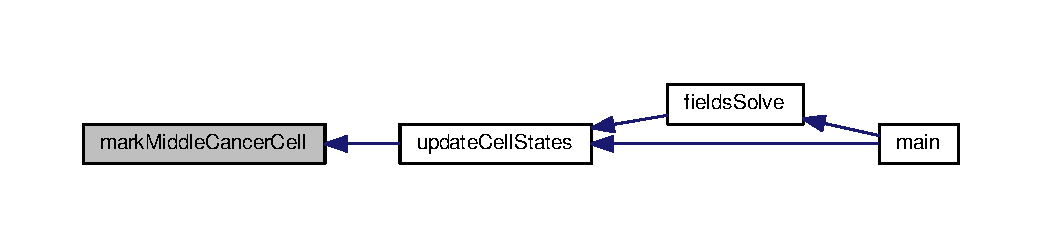
\includegraphics[width=350pt]{cells_8c_a00dbe1f9f23fc7385462c32b89d28cf8_icgraph}
\end{center}
\end{figure}


\hypertarget{cells_8c_a2d9450bd2eebb8f4d645417b92666b87}{\index{cells.\-c@{cells.\-c}!mitosis@{mitosis}}
\index{mitosis@{mitosis}!cells.c@{cells.\-c}}
\subsubsection[{mitosis}]{\setlength{\rightskip}{0pt plus 5cm}void mitosis (
\begin{DoxyParamCaption}
\item[{int}]{c}
\end{DoxyParamCaption}
)}}\label{cells_8c_a2d9450bd2eebb8f4d645417b92666b87}
This function implements mitosis of cells. 

Definition at line 266 of file cells.\-c.



References cell\-Data\-::age, cells, cg1, cg2, cm, cs, cell\-Data\-::death, cell\-Data\-::density, cell\-Data\-::g1, g1, cell\-Data\-::g2, g2, cell\-Data\-::gid, cell\-Data\-::h, h, cell\-Data\-::halo, lcnc, lg1nc, lnc, local\-I\-D, cell\-Data\-::m, m, max\-Cells\-Per\-Proc, mitrand, M\-P\-Irank, cell\-Data\-::phase, cell\-Data\-::phasetime, cell\-Data\-::s, s, sdim, cell\-Data\-::size, stop\-Run(), stream, cell\-Data\-::tumor, cell\-Data\-::v, v, velocity, x, cell\-Data\-::x, double\-Vector3d\-::x, cell\-Data\-::y, double\-Vector3d\-::y, cell\-Data\-::young, cell\-Data\-::z, and double\-Vector3d\-::z.


\begin{DoxyCode}
267 \{
268 
269   \textcolor{keywordtype}{double} sc;
270   \textcolor{keywordtype}{double} shift[3];
271 
272   \textcolor{keywordflow}{if} (\hyperlink{global_8h_a7065c019590815f10169c219f358e7d0}{lnc} + 1 > \hyperlink{global_8h_a2de426dd266cfdaaf6fb52ba3dc2740a}{maxCellsPerProc})
273     \hyperlink{utils_8c_a07dd99a04f2723be164531a7a862fb67}{stopRun}(109, NULL, \_\_FILE\_\_, \_\_LINE\_\_);
274 
275   sc = sqrt(\hyperlink{global_8h_a6015afb23ea197551ff3d503aa3426a4}{velocity}[c].\hyperlink{tempf_8c_a1780e9c70637026d6fab31f63b3a193e}{x} * \hyperlink{global_8h_a6015afb23ea197551ff3d503aa3426a4}{velocity}[c].\hyperlink{tempf_8c_a1780e9c70637026d6fab31f63b3a193e}{x} + \hyperlink{global_8h_a6015afb23ea197551ff3d503aa3426a4}{velocity}[c].y * 
      \hyperlink{global_8h_a6015afb23ea197551ff3d503aa3426a4}{velocity}[c].y +
276         \hyperlink{global_8h_a6015afb23ea197551ff3d503aa3426a4}{velocity}[c].z * \hyperlink{global_8h_a6015afb23ea197551ff3d503aa3426a4}{velocity}[c].z);
277 
278   \textcolor{comment}{/* daughter cells are shifted away from the center of parent cell */}
279   \textcolor{keywordflow}{if} (sc > 0 && \hyperlink{global_8h_a4dc71fc8b57bbbe431a4b183d56297b3}{mitrand} == 0) \{  \textcolor{comment}{/* direction of shift related to velocity vector */}
280     sc = \hyperlink{global_8h_a56da06a03aa369ca203be968cb56d16c}{cells}[c].\hyperlink{structcellData_aba3c5d750d5dbd6e86c11ecaca62885e}{size} / (2 * sc);
281     shift[0] = sc * \hyperlink{global_8h_a6015afb23ea197551ff3d503aa3426a4}{velocity}[c].\hyperlink{structdoubleVector3d_af88b946fb90d5f08b5fb740c70e98c10}{x};
282     shift[1] = sc * \hyperlink{global_8h_a6015afb23ea197551ff3d503aa3426a4}{velocity}[c].\hyperlink{structdoubleVector3d_ab927965981178aa1fba979a37168db2a}{y};
283     \textcolor{keywordflow}{if} (\hyperlink{global_8h_a2f8118c1bfdf986827e156210c33cbab}{sdim} == 3)
284       shift[2] = sc * \hyperlink{global_8h_a6015afb23ea197551ff3d503aa3426a4}{velocity}[c].\hyperlink{structdoubleVector3d_ab3e6ed577a7c669c19de1f9c1b46c872}{z};
285     \textcolor{keywordflow}{else}
286       shift[2] = 0.0;
287   \} \textcolor{keywordflow}{else} \{          \textcolor{comment}{/* direction of shift chosen randomly */}
288     \textcolor{keywordtype}{int} accept = 0;
289     \textcolor{keywordflow}{while} (accept == 0) \{
290       shift[0] = sprng(\hyperlink{global_8h_a5340130b6fb2647cef6b71354e27b0d4}{stream}) * 2.0 - 1.0;
291       shift[1] = sprng(\hyperlink{global_8h_a5340130b6fb2647cef6b71354e27b0d4}{stream}) * 2.0 - 1.0;
292       \textcolor{keywordflow}{if} (\hyperlink{global_8h_a2f8118c1bfdf986827e156210c33cbab}{sdim} == 3)
293     shift[2] = sprng(\hyperlink{global_8h_a5340130b6fb2647cef6b71354e27b0d4}{stream}) * 2.0 - 1.0;
294       \textcolor{keywordflow}{else}
295     shift[2] = 0.0;
296       sc = sqrt(pow(shift[0], 2) + pow(shift[1], 2) + pow(shift[2], 2));
297       \textcolor{keywordflow}{if} (sc == 0)
298     \textcolor{keywordflow}{continue};
299       sc = \hyperlink{global_8h_a56da06a03aa369ca203be968cb56d16c}{cells}[c].\hyperlink{structcellData_aba3c5d750d5dbd6e86c11ecaca62885e}{size} / (2 * sc);
300       shift[0] = sc * shift[0];
301       shift[1] = sc * shift[1];
302       shift[2] = sc * shift[2];
303       accept = 1;
304     \}
305   \}
306   \textcolor{comment}{/* 1st daughter cell position, size, type and age */}
307   \hyperlink{global_8h_a56da06a03aa369ca203be968cb56d16c}{cells}[\hyperlink{global_8h_a7065c019590815f10169c219f358e7d0}{lnc}].\hyperlink{structcellData_af88b946fb90d5f08b5fb740c70e98c10}{x} = \hyperlink{global_8h_a56da06a03aa369ca203be968cb56d16c}{cells}[c].\hyperlink{structcellData_af88b946fb90d5f08b5fb740c70e98c10}{x} + shift[0];
308   \hyperlink{global_8h_a56da06a03aa369ca203be968cb56d16c}{cells}[\hyperlink{global_8h_a7065c019590815f10169c219f358e7d0}{lnc}].\hyperlink{structcellData_ab927965981178aa1fba979a37168db2a}{y} = \hyperlink{global_8h_a56da06a03aa369ca203be968cb56d16c}{cells}[c].\hyperlink{structcellData_ab927965981178aa1fba979a37168db2a}{y} + shift[1];
309   \hyperlink{global_8h_a56da06a03aa369ca203be968cb56d16c}{cells}[\hyperlink{global_8h_a7065c019590815f10169c219f358e7d0}{lnc}].\hyperlink{structcellData_ab3e6ed577a7c669c19de1f9c1b46c872}{z} = \hyperlink{global_8h_a56da06a03aa369ca203be968cb56d16c}{cells}[c].\hyperlink{structcellData_ab3e6ed577a7c669c19de1f9c1b46c872}{z} + shift[2];
310   \hyperlink{global_8h_a56da06a03aa369ca203be968cb56d16c}{cells}[\hyperlink{global_8h_a7065c019590815f10169c219f358e7d0}{lnc}].\hyperlink{structcellData_aba3c5d750d5dbd6e86c11ecaca62885e}{size} = pow(2.0, -(1.0 / 3.0)) * \hyperlink{global_8h_a56da06a03aa369ca203be968cb56d16c}{cells}[c].\hyperlink{structcellData_aba3c5d750d5dbd6e86c11ecaca62885e}{size};;
311   \hyperlink{global_8h_a56da06a03aa369ca203be968cb56d16c}{cells}[\hyperlink{global_8h_a7065c019590815f10169c219f358e7d0}{lnc}].\hyperlink{structcellData_a49af8c5336d6c2401bc24f86dbb97b36}{tumor} = \hyperlink{global_8h_a56da06a03aa369ca203be968cb56d16c}{cells}[c].\hyperlink{structcellData_a49af8c5336d6c2401bc24f86dbb97b36}{tumor};
312   \hyperlink{global_8h_a56da06a03aa369ca203be968cb56d16c}{cells}[\hyperlink{global_8h_a7065c019590815f10169c219f358e7d0}{lnc}].\hyperlink{structcellData_a91d98a856bbd96810b40af3ca5cc901a}{age} = \hyperlink{global_8h_a56da06a03aa369ca203be968cb56d16c}{cells}[c].\hyperlink{structcellData_a91d98a856bbd96810b40af3ca5cc901a}{age} + 1;
313 
314   \textcolor{comment}{/* 2nd daughter cell position, size, type and age */}
315   \hyperlink{global_8h_a56da06a03aa369ca203be968cb56d16c}{cells}[c].\hyperlink{structcellData_af88b946fb90d5f08b5fb740c70e98c10}{x} -= shift[0];
316   \hyperlink{global_8h_a56da06a03aa369ca203be968cb56d16c}{cells}[c].\hyperlink{structcellData_ab927965981178aa1fba979a37168db2a}{y} -= shift[1];
317   \hyperlink{global_8h_a56da06a03aa369ca203be968cb56d16c}{cells}[c].\hyperlink{structcellData_ab3e6ed577a7c669c19de1f9c1b46c872}{z} -= shift[2];
318   \hyperlink{global_8h_a56da06a03aa369ca203be968cb56d16c}{cells}[c].\hyperlink{structcellData_aba3c5d750d5dbd6e86c11ecaca62885e}{size} = \hyperlink{global_8h_a56da06a03aa369ca203be968cb56d16c}{cells}[\hyperlink{global_8h_a7065c019590815f10169c219f358e7d0}{lnc}].\hyperlink{structcellData_aba3c5d750d5dbd6e86c11ecaca62885e}{size};;
319   \hyperlink{global_8h_a56da06a03aa369ca203be968cb56d16c}{cells}[c].\hyperlink{structcellData_a91d98a856bbd96810b40af3ca5cc901a}{age} += 1;
320 
321   \textcolor{comment}{/* 2nd daughter cell cycle phases lenghts */}
322   \textcolor{keywordflow}{if} (\hyperlink{global_8h_a56da06a03aa369ca203be968cb56d16c}{cells}[c].tumor == 1) \{
323     \hyperlink{global_8h_a56da06a03aa369ca203be968cb56d16c}{cells}[c].\hyperlink{structcellData_a581debe7d16bce9d187b97855f4e99d4}{g1} = \hyperlink{global_8h_a30dcf4c8ed197e063ec4f2e899a83724}{cg1} * (1 + (sprng(\hyperlink{global_8h_a5340130b6fb2647cef6b71354e27b0d4}{stream}) * 2 - 1) * \hyperlink{global_8h_a48d9522e58fa05906c6dba23e5745a72}{v});
324     \hyperlink{global_8h_a56da06a03aa369ca203be968cb56d16c}{cells}[c].\hyperlink{structcellData_aee9971139118d56815564304450c4775}{g2} = \hyperlink{global_8h_af69394ce4871f38be319cc1fc0d900aa}{cg2} * (1 + (sprng(\hyperlink{global_8h_a5340130b6fb2647cef6b71354e27b0d4}{stream}) * 2 - 1) * \hyperlink{global_8h_a48d9522e58fa05906c6dba23e5745a72}{v});
325     \hyperlink{global_8h_a56da06a03aa369ca203be968cb56d16c}{cells}[c].\hyperlink{structcellData_a874f74a4dc1c9a0cd9c6e0d79c298f55}{s} = \hyperlink{global_8h_abafbf12f10610688ad061edb4b911e60}{cs} * (1 + (sprng(\hyperlink{global_8h_a5340130b6fb2647cef6b71354e27b0d4}{stream}) * 2 - 1) * \hyperlink{global_8h_a48d9522e58fa05906c6dba23e5745a72}{v});
326     \hyperlink{global_8h_a56da06a03aa369ca203be968cb56d16c}{cells}[c].\hyperlink{structcellData_ac51334f57ef8b81c0629c9421798c344}{m} = \hyperlink{global_8h_a3755ba3f0c70f11bcfc3d348bf394193}{cm} * (1 + (sprng(\hyperlink{global_8h_a5340130b6fb2647cef6b71354e27b0d4}{stream}) * 2 - 1) * \hyperlink{global_8h_a48d9522e58fa05906c6dba23e5745a72}{v});
327   \} \textcolor{keywordflow}{else} \{
328     \hyperlink{global_8h_a56da06a03aa369ca203be968cb56d16c}{cells}[c].\hyperlink{structcellData_a581debe7d16bce9d187b97855f4e99d4}{g1} = \hyperlink{global_8h_a581debe7d16bce9d187b97855f4e99d4}{g1} * (1 + (sprng(\hyperlink{global_8h_a5340130b6fb2647cef6b71354e27b0d4}{stream}) * 2 - 1) * \hyperlink{global_8h_a48d9522e58fa05906c6dba23e5745a72}{v});
329     \hyperlink{global_8h_a56da06a03aa369ca203be968cb56d16c}{cells}[c].\hyperlink{structcellData_aee9971139118d56815564304450c4775}{g2} = \hyperlink{global_8h_aee9971139118d56815564304450c4775}{g2} * (1 + (sprng(\hyperlink{global_8h_a5340130b6fb2647cef6b71354e27b0d4}{stream}) * 2 - 1) * \hyperlink{global_8h_a48d9522e58fa05906c6dba23e5745a72}{v});
330     \hyperlink{global_8h_a56da06a03aa369ca203be968cb56d16c}{cells}[c].\hyperlink{structcellData_a874f74a4dc1c9a0cd9c6e0d79c298f55}{s} = \hyperlink{global_8h_a874f74a4dc1c9a0cd9c6e0d79c298f55}{s} * (1 + (sprng(\hyperlink{global_8h_a5340130b6fb2647cef6b71354e27b0d4}{stream}) * 2 - 1) * \hyperlink{global_8h_a48d9522e58fa05906c6dba23e5745a72}{v});
331     \hyperlink{global_8h_a56da06a03aa369ca203be968cb56d16c}{cells}[c].\hyperlink{structcellData_ac51334f57ef8b81c0629c9421798c344}{m} = \hyperlink{global_8h_ac51334f57ef8b81c0629c9421798c344}{m} * (1 + (sprng(\hyperlink{global_8h_a5340130b6fb2647cef6b71354e27b0d4}{stream}) * 2 - 1) * \hyperlink{global_8h_a48d9522e58fa05906c6dba23e5745a72}{v});
332   \}
333   \textcolor{comment}{/* 1st daughter cell global ID */}
334   \hyperlink{global_8h_a56da06a03aa369ca203be968cb56d16c}{cells}[\hyperlink{global_8h_a7065c019590815f10169c219f358e7d0}{lnc}].\hyperlink{structcellData_abb4d4bd9231e9f994e87f32cc4fcfce8}{gid} =
335       (\textcolor{keywordtype}{unsigned} \textcolor{keywordtype}{long} \textcolor{keywordtype}{long} int) \hyperlink{global_8h_a710288ab7d2734acc4566a87a645325d}{MPIrank} *(\textcolor{keywordtype}{unsigned} \textcolor{keywordtype}{long} \textcolor{keywordtype}{long} \textcolor{keywordtype}{int})
336       \hyperlink{global_8h_a2de426dd266cfdaaf6fb52ba3dc2740a}{maxCellsPerProc} + (\textcolor{keywordtype}{unsigned} \textcolor{keywordtype}{long} \textcolor{keywordtype}{long} int) \hyperlink{global_8h_a7065c019590815f10169c219f358e7d0}{lnc};
337 
338   \textcolor{comment}{/* 1st daughter cell parameters */}
339   \hyperlink{global_8h_a56da06a03aa369ca203be968cb56d16c}{cells}[\hyperlink{global_8h_a7065c019590815f10169c219f358e7d0}{lnc}].\hyperlink{structcellData_a3b90d5a73541ab9402511d87bed076ef}{v} = 0.0;
340   \hyperlink{global_8h_a56da06a03aa369ca203be968cb56d16c}{cells}[\hyperlink{global_8h_a7065c019590815f10169c219f358e7d0}{lnc}].\hyperlink{structcellData_a6f8c052f8417728038991f7f2826d38d}{density} = \hyperlink{global_8h_a56da06a03aa369ca203be968cb56d16c}{cells}[c].\hyperlink{structcellData_a6f8c052f8417728038991f7f2826d38d}{density};
341   \hyperlink{global_8h_a56da06a03aa369ca203be968cb56d16c}{cells}[\hyperlink{global_8h_a7065c019590815f10169c219f358e7d0}{lnc}].\hyperlink{structcellData_a8ee9be1b5aa75abae556de3088cba6d9}{h} = \hyperlink{global_8h_a8ee9be1b5aa75abae556de3088cba6d9}{h};
342   \hyperlink{global_8h_a56da06a03aa369ca203be968cb56d16c}{cells}[\hyperlink{global_8h_a7065c019590815f10169c219f358e7d0}{lnc}].\hyperlink{structcellData_ad0bd87a264e65d1c17ecc07049819f2c}{young} = 2100.0 + sprng(\hyperlink{global_8h_a5340130b6fb2647cef6b71354e27b0d4}{stream}) * 100.0;
343   \hyperlink{global_8h_a56da06a03aa369ca203be968cb56d16c}{cells}[\hyperlink{global_8h_a7065c019590815f10169c219f358e7d0}{lnc}].\hyperlink{structcellData_a80ff3fcc4d03d0b1b01559839d12df5b}{halo} = 0;
344   \hyperlink{global_8h_a56da06a03aa369ca203be968cb56d16c}{cells}[\hyperlink{global_8h_a7065c019590815f10169c219f358e7d0}{lnc}].\hyperlink{structcellData_accf3aec63bc20b3c99ab4881cb07c05b}{phase} = 1;
345   \hyperlink{global_8h_a56da06a03aa369ca203be968cb56d16c}{cells}[\hyperlink{global_8h_a7065c019590815f10169c219f358e7d0}{lnc}].\hyperlink{structcellData_add1e1533be6e693ffedcdbafdf8b855c}{death} = 0;
346   \hyperlink{global_8h_a56da06a03aa369ca203be968cb56d16c}{cells}[\hyperlink{global_8h_a7065c019590815f10169c219f358e7d0}{lnc}].\hyperlink{structcellData_afe1297f954440c453b59fcb06992dbd5}{phasetime} = 0.0;
347   \textcolor{comment}{/* 1st daughter cell cycle phases lenghts */}
348   \textcolor{keywordflow}{if} (\hyperlink{global_8h_a56da06a03aa369ca203be968cb56d16c}{cells}[\hyperlink{global_8h_a7065c019590815f10169c219f358e7d0}{lnc}].tumor == 1) \{
349     \hyperlink{global_8h_a56da06a03aa369ca203be968cb56d16c}{cells}[\hyperlink{global_8h_a7065c019590815f10169c219f358e7d0}{lnc}].\hyperlink{structcellData_a581debe7d16bce9d187b97855f4e99d4}{g1} = \hyperlink{global_8h_a30dcf4c8ed197e063ec4f2e899a83724}{cg1} * (1 + (sprng(\hyperlink{global_8h_a5340130b6fb2647cef6b71354e27b0d4}{stream}) * 2 - 1) * \hyperlink{global_8h_a48d9522e58fa05906c6dba23e5745a72}{v});
350     \hyperlink{global_8h_a56da06a03aa369ca203be968cb56d16c}{cells}[\hyperlink{global_8h_a7065c019590815f10169c219f358e7d0}{lnc}].\hyperlink{structcellData_aee9971139118d56815564304450c4775}{g2} = \hyperlink{global_8h_af69394ce4871f38be319cc1fc0d900aa}{cg2} * (1 + (sprng(\hyperlink{global_8h_a5340130b6fb2647cef6b71354e27b0d4}{stream}) * 2 - 1) * \hyperlink{global_8h_a48d9522e58fa05906c6dba23e5745a72}{v});
351     \hyperlink{global_8h_a56da06a03aa369ca203be968cb56d16c}{cells}[\hyperlink{global_8h_a7065c019590815f10169c219f358e7d0}{lnc}].\hyperlink{structcellData_a874f74a4dc1c9a0cd9c6e0d79c298f55}{s} = \hyperlink{global_8h_abafbf12f10610688ad061edb4b911e60}{cs} * (1 + (sprng(\hyperlink{global_8h_a5340130b6fb2647cef6b71354e27b0d4}{stream}) * 2 - 1) * \hyperlink{global_8h_a48d9522e58fa05906c6dba23e5745a72}{v});
352     \hyperlink{global_8h_a56da06a03aa369ca203be968cb56d16c}{cells}[\hyperlink{global_8h_a7065c019590815f10169c219f358e7d0}{lnc}].\hyperlink{structcellData_ac51334f57ef8b81c0629c9421798c344}{m} = \hyperlink{global_8h_a3755ba3f0c70f11bcfc3d348bf394193}{cm} * (1 + (sprng(\hyperlink{global_8h_a5340130b6fb2647cef6b71354e27b0d4}{stream}) * 2 - 1) * \hyperlink{global_8h_a48d9522e58fa05906c6dba23e5745a72}{v});
353   \} \textcolor{keywordflow}{else} \{
354     \hyperlink{global_8h_a56da06a03aa369ca203be968cb56d16c}{cells}[\hyperlink{global_8h_a7065c019590815f10169c219f358e7d0}{lnc}].\hyperlink{structcellData_a581debe7d16bce9d187b97855f4e99d4}{g1} = \hyperlink{global_8h_a581debe7d16bce9d187b97855f4e99d4}{g1} * (1 + (sprng(\hyperlink{global_8h_a5340130b6fb2647cef6b71354e27b0d4}{stream}) * 2 - 1) * \hyperlink{global_8h_a48d9522e58fa05906c6dba23e5745a72}{v});
355     \hyperlink{global_8h_a56da06a03aa369ca203be968cb56d16c}{cells}[\hyperlink{global_8h_a7065c019590815f10169c219f358e7d0}{lnc}].\hyperlink{structcellData_aee9971139118d56815564304450c4775}{g2} = \hyperlink{global_8h_aee9971139118d56815564304450c4775}{g2} * (1 + (sprng(\hyperlink{global_8h_a5340130b6fb2647cef6b71354e27b0d4}{stream}) * 2 - 1) * \hyperlink{global_8h_a48d9522e58fa05906c6dba23e5745a72}{v});
356     \hyperlink{global_8h_a56da06a03aa369ca203be968cb56d16c}{cells}[\hyperlink{global_8h_a7065c019590815f10169c219f358e7d0}{lnc}].\hyperlink{structcellData_a874f74a4dc1c9a0cd9c6e0d79c298f55}{s} = \hyperlink{global_8h_a874f74a4dc1c9a0cd9c6e0d79c298f55}{s} * (1 + (sprng(\hyperlink{global_8h_a5340130b6fb2647cef6b71354e27b0d4}{stream}) * 2 - 1) * \hyperlink{global_8h_a48d9522e58fa05906c6dba23e5745a72}{v});
357     \hyperlink{global_8h_a56da06a03aa369ca203be968cb56d16c}{cells}[\hyperlink{global_8h_a7065c019590815f10169c219f358e7d0}{lnc}].\hyperlink{structcellData_ac51334f57ef8b81c0629c9421798c344}{m} = \hyperlink{global_8h_ac51334f57ef8b81c0629c9421798c344}{m} * (1 + (sprng(\hyperlink{global_8h_a5340130b6fb2647cef6b71354e27b0d4}{stream}) * 2 - 1) * \hyperlink{global_8h_a48d9522e58fa05906c6dba23e5745a72}{v});
358   \}
359 
360   \textcolor{comment}{/* update local cell counters */}
361   \textcolor{keywordflow}{if} (\hyperlink{global_8h_a56da06a03aa369ca203be968cb56d16c}{cells}[\hyperlink{global_8h_a7065c019590815f10169c219f358e7d0}{lnc}].tumor == 1)
362     \hyperlink{global_8h_ab67f763fa0f30ce2912a6ab60dc8e648}{lcnc} += 1;
363   \hyperlink{global_8h_a7065c019590815f10169c219f358e7d0}{lnc} = \hyperlink{global_8h_a7065c019590815f10169c219f358e7d0}{lnc} + 1;
364   \hyperlink{global_8h_a59dc7e07b6be86e29bd0e9f3f18c3ca2}{lg1nc} += 1;
365   \textcolor{comment}{/* increment local ID */}
366   \hyperlink{global_8h_a265cb7ee626de517ecec0f0ac60833a7}{localID}++;
367 
368 \}
\end{DoxyCode}


Here is the call graph for this function\-:\nopagebreak
\begin{figure}[H]
\begin{center}
\leavevmode
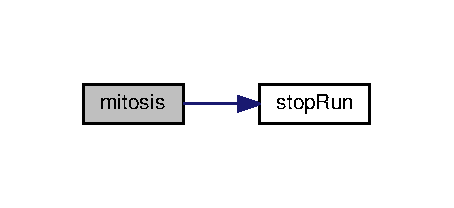
\includegraphics[width=218pt]{cells_8c_a2d9450bd2eebb8f4d645417b92666b87_cgraph}
\end{center}
\end{figure}




Here is the caller graph for this function\-:\nopagebreak
\begin{figure}[H]
\begin{center}
\leavevmode
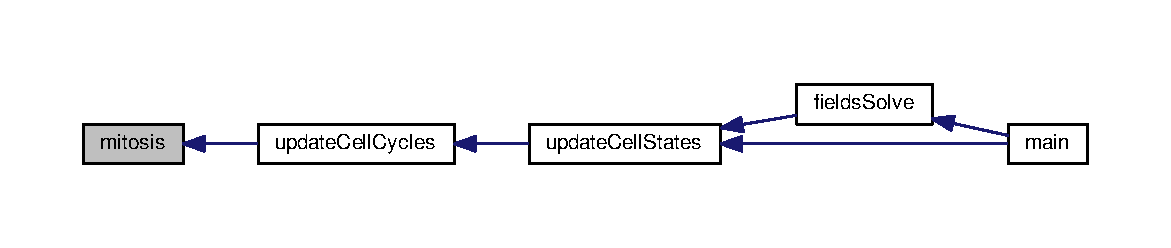
\includegraphics[width=350pt]{cells_8c_a2d9450bd2eebb8f4d645417b92666b87_icgraph}
\end{center}
\end{figure}


\hypertarget{cells_8c_aeeb6dee9938af6fef987f1c949458703}{\index{cells.\-c@{cells.\-c}!update\-Cell\-Counters@{update\-Cell\-Counters}}
\index{update\-Cell\-Counters@{update\-Cell\-Counters}!cells.c@{cells.\-c}}
\subsubsection[{update\-Cell\-Counters}]{\setlength{\rightskip}{0pt plus 5cm}void update\-Cell\-Counters (
\begin{DoxyParamCaption}
{}
\end{DoxyParamCaption}
)}}\label{cells_8c_aeeb6dee9938af6fef987f1c949458703}
This function updates cell counters. 

Definition at line 493 of file cells.\-c.



References lnc, local\-Cell\-Count, number\-Of\-Counts, tlnc, and total\-Cell\-Count.


\begin{DoxyCode}
494 \{
495   MPI\_Allgather(&\hyperlink{global_8h_a7065c019590815f10169c219f358e7d0}{lnc}, 1, MPI\_INT64\_T, \hyperlink{global_8h_ac3c96b975a3376c555ad22a7d2688b2f}{tlnc}, 1, MPI\_INT64\_T,
496         MPI\_COMM\_WORLD);
497   MPI\_Allreduce(\hyperlink{global_8h_a055fa0d3ee8b74712109365cf2802bfa}{localCellCount}, \hyperlink{global_8h_af1a14df9e6c8efece5183d9625039587}{totalCellCount}, 
      \hyperlink{global_8h_a97c5d6b146e57ace62a66400c433aa4d}{numberOfCounts},
498         MPI\_INT64\_T, MPI\_SUM, MPI\_COMM\_WORLD);
499 \}
\end{DoxyCode}


Here is the caller graph for this function\-:\nopagebreak
\begin{figure}[H]
\begin{center}
\leavevmode
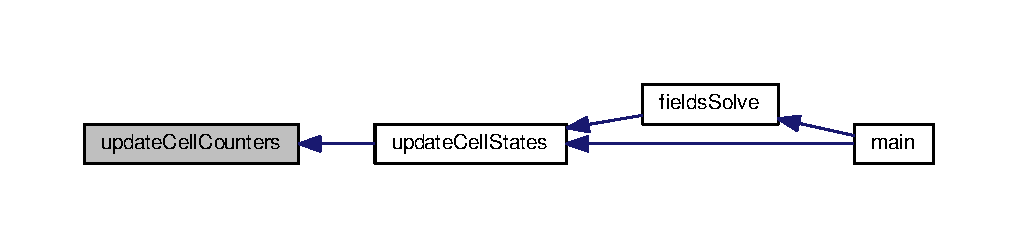
\includegraphics[width=350pt]{cells_8c_aeeb6dee9938af6fef987f1c949458703_icgraph}
\end{center}
\end{figure}


\hypertarget{cells_8c_a718a88fce87f8ebdb87ed2fafed4c5c4}{\index{cells.\-c@{cells.\-c}!update\-Cell\-Cycles@{update\-Cell\-Cycles}}
\index{update\-Cell\-Cycles@{update\-Cell\-Cycles}!cells.c@{cells.\-c}}
\subsubsection[{update\-Cell\-Cycles}]{\setlength{\rightskip}{0pt plus 5cm}int update\-Cell\-Cycles (
\begin{DoxyParamCaption}
{}
\end{DoxyParamCaption}
)}}\label{cells_8c_a718a88fce87f8ebdb87ed2fafed4c5c4}
This function updates cells' cycle phases. 

Definition at line 537 of file cells.\-c.



References celld, cell\-Fields, cells, csize, density\-Critical\-Level1, density\-Critical\-Level2, field\-Critical\-Level1, field\-Critical\-Level2, cell\-Data\-::g1, g1, g2, gf\-Dt, gfields, lg0nc, lg1nc, lg2nc, lmnc, lnc, lnnc, lsnc, m, mitosis(), nc, O\-X\-Y\-G, oxygen, cell\-Data\-::phase, cell\-Data\-::phasetime, rd, rsum, s, sim\-Start, cell\-Data\-::size, and stream.


\begin{DoxyCode}
538 \{
539 
540   \textcolor{keywordtype}{int} c;
541   \textcolor{keywordtype}{double} eps, epsCancer;
542   \textcolor{keywordtype}{int} lncAtThisStep;
543 
544   eps = \hyperlink{global_8h_a8a758046e5cb8b72210f0fc18cb3b7e1}{densityCriticalLevel1};
545   epsCancer = \hyperlink{global_8h_aeddd5065a64a6a39c79e1dab7c0f9edf}{densityCriticalLevel2};
546 
547   lncAtThisStep = \hyperlink{global_8h_a7065c019590815f10169c219f358e7d0}{lnc};
548 
549   \textcolor{keywordflow}{for} (c = 0; c < lncAtThisStep; c++) \{
550 
551     \textcolor{keywordflow}{if} (outsideTheBox(c)) \{
552       \hyperlink{cells_8c_a96a825c021fe648b7fb171bd2c532ffb}{celld}[c] = 1;
553       \hyperlink{global_8h_a087a95bb36c9b36c708a73ce656fd1f1}{rsum}++;
554       \textcolor{keywordflow}{continue};
555     \}
556 
557     \textcolor{keywordflow}{if} (\hyperlink{cells_8c_a96a825c021fe648b7fb171bd2c532ffb}{celld}[c])
558       \textcolor{keywordflow}{continue};
559 
560     \textcolor{keywordflow}{if} (\hyperlink{global_8h_a42a935b4eec9242e09d47fc1c2b6dba3}{simStart}) \{
561 
562       \textcolor{keywordflow}{if} (\hyperlink{global_8h_a56da06a03aa369ca203be968cb56d16c}{cells}[c].phase != 0
563       && ((\hyperlink{global_8h_a56da06a03aa369ca203be968cb56d16c}{cells}[c].tumor == 0 && \hyperlink{global_8h_a56da06a03aa369ca203be968cb56d16c}{cells}[c].density <= eps)
564           || (\hyperlink{global_8h_a56da06a03aa369ca203be968cb56d16c}{cells}[c].tumor == 1 && \hyperlink{global_8h_a56da06a03aa369ca203be968cb56d16c}{cells}[c].density <= epsCancer)))
565     \hyperlink{global_8h_a56da06a03aa369ca203be968cb56d16c}{cells}[c].\hyperlink{structcellData_afe1297f954440c453b59fcb06992dbd5}{phasetime} += \hyperlink{global_8h_aae6a1dda703fb50b7a8b0f4dc01d82c1}{gfDt} / 3600.0;
566 
567       \textcolor{keywordflow}{switch} (\hyperlink{global_8h_a56da06a03aa369ca203be968cb56d16c}{cells}[c].phase) \{
568 
569       \textcolor{keywordflow}{case} 0:           \textcolor{comment}{/* G0 phase */}
570     \textcolor{keywordflow}{if} (\hyperlink{fields_8h_abe4692639a5f11507faff09f2d37efa8}{gfields} && \hyperlink{fields_8h_a67dd60f843bcdd47eb1503456d0da5de}{oxygen}
571         && \hyperlink{global_8h_a25e4317a1b5bb95a8e71e0e8c4e11f2b}{cellFields}[\hyperlink{fields_8h_a5e74e9586fb0eac40835526c74bcb0bc}{OXYG}][c] < \hyperlink{fields_8h_a5534681dc803f20910d872026257fd75}{fieldCriticalLevel2}[
      \hyperlink{fields_8h_a5e74e9586fb0eac40835526c74bcb0bc}{OXYG}]) \{
572       \hyperlink{global_8h_a56da06a03aa369ca203be968cb56d16c}{cells}[c].\hyperlink{structcellData_accf3aec63bc20b3c99ab4881cb07c05b}{phase} = 5;
573       \hyperlink{global_8h_a56da06a03aa369ca203be968cb56d16c}{cells}[c].\hyperlink{structcellData_afe1297f954440c453b59fcb06992dbd5}{phasetime} = 0;
574       \hyperlink{global_8h_a356af225353f2a5512be222c1354bee3}{lg0nc}--;
575       \hyperlink{global_8h_a97370c479716d79f799616103c487d51}{lnnc}++;
576       \textcolor{keywordflow}{break};
577     \}
578     \textcolor{comment}{/* transition to G1 phase */}
579     \textcolor{keywordflow}{if} ((\hyperlink{global_8h_a56da06a03aa369ca203be968cb56d16c}{cells}[c].tumor == 0 && \hyperlink{global_8h_a56da06a03aa369ca203be968cb56d16c}{cells}[c].density <= eps) ||   \textcolor{comment}{/* enough space for healthy cell */}
580         (\hyperlink{global_8h_a56da06a03aa369ca203be968cb56d16c}{cells}[c].tumor == 1 && \hyperlink{global_8h_a56da06a03aa369ca203be968cb56d16c}{cells}[c].density <= epsCancer) || \textcolor{comment}{/* enough space for tumor cell 
      */}
581         \hyperlink{global_8h_a0845b4b004824f1fe3cd69db1672fa15}{nc} == 1 ||        \textcolor{comment}{/* only single cell in the simulation */}
582         (\hyperlink{fields_8h_abe4692639a5f11507faff09f2d37efa8}{gfields} && \hyperlink{fields_8h_a67dd60f843bcdd47eb1503456d0da5de}{oxygen} && \hyperlink{global_8h_a25e4317a1b5bb95a8e71e0e8c4e11f2b}{cellFields}[OXYG][c] >= 
      \hyperlink{fields_8h_a3d0360f40f207ac596765b891c46b285}{fieldCriticalLevel1}[OXYG])) \{    \textcolor{comment}{/* sufficient level of oxygen */}
583       \hyperlink{global_8h_a56da06a03aa369ca203be968cb56d16c}{cells}[c].\hyperlink{structcellData_accf3aec63bc20b3c99ab4881cb07c05b}{phase} = 1;
584       \hyperlink{global_8h_a356af225353f2a5512be222c1354bee3}{lg0nc}--;
585       \hyperlink{global_8h_a59dc7e07b6be86e29bd0e9f3f18c3ca2}{lg1nc}++;
586       \textcolor{keywordflow}{break};
587     \}
588     \textcolor{keywordflow}{break};
589       \textcolor{keywordflow}{case} 1:           \textcolor{comment}{/* G1 phase */}
590     \textcolor{comment}{/* transition to G0 or Necrotic phase */}
591     \textcolor{keywordflow}{if} ((\hyperlink{global_8h_a56da06a03aa369ca203be968cb56d16c}{cells}[c].tumor == 0 && \hyperlink{global_8h_a56da06a03aa369ca203be968cb56d16c}{cells}[c].density > eps) ||    \textcolor{comment}{/* too crowdy for healthy cell */}
592         (\hyperlink{global_8h_a56da06a03aa369ca203be968cb56d16c}{cells}[c].tumor == 1 && \hyperlink{global_8h_a56da06a03aa369ca203be968cb56d16c}{cells}[c].density > epsCancer) ||  \textcolor{comment}{/* too crowdy for tumor cell */}
593         (\hyperlink{fields_8h_abe4692639a5f11507faff09f2d37efa8}{gfields} && \hyperlink{fields_8h_a67dd60f843bcdd47eb1503456d0da5de}{oxygen} && \hyperlink{global_8h_a25e4317a1b5bb95a8e71e0e8c4e11f2b}{cellFields}[OXYG][c] < 
      \hyperlink{fields_8h_a3d0360f40f207ac596765b891c46b285}{fieldCriticalLevel1}[OXYG])) \{    \textcolor{comment}{/* too low oxygen level */}
594       \textcolor{keywordflow}{if} (\hyperlink{fields_8h_abe4692639a5f11507faff09f2d37efa8}{gfields} && \hyperlink{fields_8h_a67dd60f843bcdd47eb1503456d0da5de}{oxygen} && \hyperlink{global_8h_a25e4317a1b5bb95a8e71e0e8c4e11f2b}{cellFields}[OXYG][c] < 
      \hyperlink{fields_8h_a5534681dc803f20910d872026257fd75}{fieldCriticalLevel2}[OXYG]) \{ \textcolor{comment}{/* transition to Necrotic phase */}
595         \hyperlink{global_8h_a56da06a03aa369ca203be968cb56d16c}{cells}[c].\hyperlink{structcellData_accf3aec63bc20b3c99ab4881cb07c05b}{phase} = 5;
596         \hyperlink{global_8h_a56da06a03aa369ca203be968cb56d16c}{cells}[c].\hyperlink{structcellData_afe1297f954440c453b59fcb06992dbd5}{phasetime} = 0;
597         \hyperlink{global_8h_a59dc7e07b6be86e29bd0e9f3f18c3ca2}{lg1nc}--;
598         \hyperlink{global_8h_a97370c479716d79f799616103c487d51}{lnnc}++;
599       \} \textcolor{keywordflow}{else} \{      \textcolor{comment}{/* transition to G0 phase */}
600         \hyperlink{global_8h_a56da06a03aa369ca203be968cb56d16c}{cells}[c].\hyperlink{structcellData_accf3aec63bc20b3c99ab4881cb07c05b}{phase} = 0;
601         \hyperlink{global_8h_a59dc7e07b6be86e29bd0e9f3f18c3ca2}{lg1nc}--;
602         \hyperlink{global_8h_a356af225353f2a5512be222c1354bee3}{lg0nc}++;
603       \}
604       \textcolor{keywordflow}{break};
605     \}
606     \textcolor{comment}{/* cells grow in phase G1 */}
607     \textcolor{keywordflow}{if} (\hyperlink{global_8h_a56da06a03aa369ca203be968cb56d16c}{cells}[c].size < \hyperlink{global_8h_a3b735e8520f1816ee73ee50daa3ef756}{csize}) \{
608       \hyperlink{global_8h_a56da06a03aa369ca203be968cb56d16c}{cells}[c].\hyperlink{structcellData_aba3c5d750d5dbd6e86c11ecaca62885e}{size} +=
609           (\hyperlink{global_8h_a3b735e8520f1816ee73ee50daa3ef756}{csize} -
610            pow(2.0,
611            -(1.0 / 3.0)) * \hyperlink{global_8h_a3b735e8520f1816ee73ee50daa3ef756}{csize}) * (\hyperlink{global_8h_aae6a1dda703fb50b7a8b0f4dc01d82c1}{gfDt}) / (3600.0 *
612                               \hyperlink{global_8h_a56da06a03aa369ca203be968cb56d16c}{cells}[c].\hyperlink{structcellData_a581debe7d16bce9d187b97855f4e99d4}{g1});
613     \}
614     \textcolor{keywordflow}{if} (\hyperlink{global_8h_a56da06a03aa369ca203be968cb56d16c}{cells}[c].size > \hyperlink{global_8h_a3b735e8520f1816ee73ee50daa3ef756}{csize})
615       \hyperlink{global_8h_a56da06a03aa369ca203be968cb56d16c}{cells}[c].\hyperlink{structcellData_aba3c5d750d5dbd6e86c11ecaca62885e}{size} = \hyperlink{global_8h_a3b735e8520f1816ee73ee50daa3ef756}{csize};
616     \textcolor{keywordflow}{if} (\hyperlink{global_8h_a56da06a03aa369ca203be968cb56d16c}{cells}[c].phasetime >= \hyperlink{global_8h_a56da06a03aa369ca203be968cb56d16c}{cells}[c].\hyperlink{global_8h_a581debe7d16bce9d187b97855f4e99d4}{g1}) \{
617       \textcolor{keywordtype}{int} death;
618       \hyperlink{global_8h_a56da06a03aa369ca203be968cb56d16c}{cells}[c].\hyperlink{structcellData_accf3aec63bc20b3c99ab4881cb07c05b}{phase} = 2;
619       \hyperlink{global_8h_a56da06a03aa369ca203be968cb56d16c}{cells}[c].\hyperlink{structcellData_afe1297f954440c453b59fcb06992dbd5}{phasetime} = 0;
620       \hyperlink{global_8h_a59dc7e07b6be86e29bd0e9f3f18c3ca2}{lg1nc}--;
621       \hyperlink{global_8h_af5e326c959f5815222d8f8e3f4d66419}{lsnc}++;
622       \textcolor{keywordflow}{if} (\hyperlink{global_8h_a56da06a03aa369ca203be968cb56d16c}{cells}[c].tumor == 0) \{
623         death = (sprng(\hyperlink{global_8h_a5340130b6fb2647cef6b71354e27b0d4}{stream}) < \hyperlink{global_8h_a0d2a1379adf81ce5f962f3c9263e81e9}{rd} ? 1 : 0);
624         \textcolor{keywordflow}{if} (death) \{
625           \hyperlink{cells_8c_a96a825c021fe648b7fb171bd2c532ffb}{celld}[c] = 1;
626           \hyperlink{global_8h_a087a95bb36c9b36c708a73ce656fd1f1}{rsum}++;
627         \}
628       \}
629     \}
630     \textcolor{keywordflow}{break};
631       \textcolor{keywordflow}{case} 2:           \textcolor{comment}{/* S phase */}
632     \textcolor{keywordflow}{if} (\hyperlink{fields_8h_abe4692639a5f11507faff09f2d37efa8}{gfields} && \hyperlink{fields_8h_a67dd60f843bcdd47eb1503456d0da5de}{oxygen}
633         && \hyperlink{global_8h_a25e4317a1b5bb95a8e71e0e8c4e11f2b}{cellFields}[OXYG][c] < \hyperlink{fields_8h_a5534681dc803f20910d872026257fd75}{fieldCriticalLevel2}[OXYG]) \{
634       \hyperlink{global_8h_a56da06a03aa369ca203be968cb56d16c}{cells}[c].\hyperlink{structcellData_accf3aec63bc20b3c99ab4881cb07c05b}{phase} = 5;
635       \hyperlink{global_8h_a56da06a03aa369ca203be968cb56d16c}{cells}[c].\hyperlink{structcellData_afe1297f954440c453b59fcb06992dbd5}{phasetime} = 0;
636       \hyperlink{global_8h_af5e326c959f5815222d8f8e3f4d66419}{lsnc}--;
637       \hyperlink{global_8h_a97370c479716d79f799616103c487d51}{lnnc}++;
638       \textcolor{keywordflow}{break};
639     \}
640     \textcolor{keywordflow}{if} (\hyperlink{global_8h_a56da06a03aa369ca203be968cb56d16c}{cells}[c].phasetime >= \hyperlink{global_8h_a56da06a03aa369ca203be968cb56d16c}{cells}[c].\hyperlink{global_8h_a874f74a4dc1c9a0cd9c6e0d79c298f55}{s}) \{
641       \hyperlink{global_8h_a56da06a03aa369ca203be968cb56d16c}{cells}[c].\hyperlink{structcellData_accf3aec63bc20b3c99ab4881cb07c05b}{phase} = 3;
642       \hyperlink{global_8h_a56da06a03aa369ca203be968cb56d16c}{cells}[c].\hyperlink{structcellData_afe1297f954440c453b59fcb06992dbd5}{phasetime} = 0;
643       \hyperlink{global_8h_af5e326c959f5815222d8f8e3f4d66419}{lsnc}--;
644       \hyperlink{global_8h_a17ca9380dca478aa01c68ce4cc8ca720}{lg2nc}++;
645       \textcolor{keywordflow}{break};
646     \}
647     \textcolor{keywordflow}{break};
648       \textcolor{keywordflow}{case} 3:           \textcolor{comment}{/* G2 phase */}
649     \textcolor{keywordflow}{if} (\hyperlink{fields_8h_abe4692639a5f11507faff09f2d37efa8}{gfields} && \hyperlink{fields_8h_a67dd60f843bcdd47eb1503456d0da5de}{oxygen}
650         && \hyperlink{global_8h_a25e4317a1b5bb95a8e71e0e8c4e11f2b}{cellFields}[OXYG][c] < \hyperlink{fields_8h_a5534681dc803f20910d872026257fd75}{fieldCriticalLevel2}[OXYG]) \{
651       \hyperlink{global_8h_a56da06a03aa369ca203be968cb56d16c}{cells}[c].\hyperlink{structcellData_accf3aec63bc20b3c99ab4881cb07c05b}{phase} = 5;
652       \hyperlink{global_8h_a56da06a03aa369ca203be968cb56d16c}{cells}[c].\hyperlink{structcellData_afe1297f954440c453b59fcb06992dbd5}{phasetime} = 0;
653       \hyperlink{global_8h_a17ca9380dca478aa01c68ce4cc8ca720}{lg2nc}--;
654       \hyperlink{global_8h_a97370c479716d79f799616103c487d51}{lnnc}++;
655       \textcolor{keywordflow}{break};
656     \}
657     \textcolor{keywordflow}{if} (\hyperlink{global_8h_a56da06a03aa369ca203be968cb56d16c}{cells}[c].phasetime >= \hyperlink{global_8h_a56da06a03aa369ca203be968cb56d16c}{cells}[c].\hyperlink{global_8h_aee9971139118d56815564304450c4775}{g2}) \{
658       \textcolor{keywordtype}{int} death;
659       \hyperlink{global_8h_a56da06a03aa369ca203be968cb56d16c}{cells}[c].\hyperlink{structcellData_accf3aec63bc20b3c99ab4881cb07c05b}{phase} = 4;
660       \hyperlink{global_8h_a56da06a03aa369ca203be968cb56d16c}{cells}[c].\hyperlink{structcellData_afe1297f954440c453b59fcb06992dbd5}{phasetime} = 0;
661       \hyperlink{global_8h_a17ca9380dca478aa01c68ce4cc8ca720}{lg2nc}--;
662       \hyperlink{global_8h_a002cff2ccc4cfc5b5f85ac5ea285ef9c}{lmnc}++;
663       \textcolor{keywordflow}{if} (\hyperlink{global_8h_a56da06a03aa369ca203be968cb56d16c}{cells}[c].tumor == 0) \{
664         death = (sprng(\hyperlink{global_8h_a5340130b6fb2647cef6b71354e27b0d4}{stream}) < \hyperlink{global_8h_a0d2a1379adf81ce5f962f3c9263e81e9}{rd} ? 1 : 0);
665         \textcolor{keywordflow}{if} (death) \{
666           \hyperlink{cells_8c_a96a825c021fe648b7fb171bd2c532ffb}{celld}[c] = 1;
667           \hyperlink{global_8h_a087a95bb36c9b36c708a73ce656fd1f1}{rsum}++;
668         \}
669       \}
670       \textcolor{keywordflow}{break};
671     \}
672     \textcolor{keywordflow}{break};
673       \textcolor{keywordflow}{case} 4:           \textcolor{comment}{/* M phase */}
674     \textcolor{keywordflow}{if} (\hyperlink{fields_8h_abe4692639a5f11507faff09f2d37efa8}{gfields} && \hyperlink{fields_8h_a67dd60f843bcdd47eb1503456d0da5de}{oxygen}
675         && \hyperlink{global_8h_a25e4317a1b5bb95a8e71e0e8c4e11f2b}{cellFields}[OXYG][c] < \hyperlink{fields_8h_a5534681dc803f20910d872026257fd75}{fieldCriticalLevel2}[OXYG]) \{
676       \hyperlink{global_8h_a56da06a03aa369ca203be968cb56d16c}{cells}[c].\hyperlink{structcellData_accf3aec63bc20b3c99ab4881cb07c05b}{phase} = 5;
677       \hyperlink{global_8h_a56da06a03aa369ca203be968cb56d16c}{cells}[c].\hyperlink{structcellData_afe1297f954440c453b59fcb06992dbd5}{phasetime} = 0;
678       \hyperlink{global_8h_a002cff2ccc4cfc5b5f85ac5ea285ef9c}{lmnc}--;
679       \hyperlink{global_8h_a97370c479716d79f799616103c487d51}{lnnc}++;
680 
681     \} \textcolor{keywordflow}{else} \textcolor{keywordflow}{if} (\hyperlink{global_8h_a56da06a03aa369ca203be968cb56d16c}{cells}[c].phasetime >= \hyperlink{global_8h_a56da06a03aa369ca203be968cb56d16c}{cells}[c].\hyperlink{global_8h_ac51334f57ef8b81c0629c9421798c344}{m}) \{
682       \hyperlink{cells_8c_a2d9450bd2eebb8f4d645417b92666b87}{mitosis}(c);
683       \hyperlink{global_8h_a56da06a03aa369ca203be968cb56d16c}{cells}[c].\hyperlink{structcellData_accf3aec63bc20b3c99ab4881cb07c05b}{phase} = 1;
684       \hyperlink{global_8h_a56da06a03aa369ca203be968cb56d16c}{cells}[c].\hyperlink{structcellData_afe1297f954440c453b59fcb06992dbd5}{phasetime} = 0;
685       \hyperlink{global_8h_a002cff2ccc4cfc5b5f85ac5ea285ef9c}{lmnc}--;
686       \hyperlink{global_8h_a59dc7e07b6be86e29bd0e9f3f18c3ca2}{lg1nc}++;
687     \}
688     \textcolor{keywordflow}{break};
689       \}             \textcolor{comment}{// switch}
690     \}               \textcolor{comment}{// if}
691   \}             \textcolor{comment}{// for loop}
692 
693   \textcolor{comment}{/* update global number of cells */}
694   MPI\_Allreduce(&\hyperlink{global_8h_a7065c019590815f10169c219f358e7d0}{lnc}, &\hyperlink{global_8h_a0845b4b004824f1fe3cd69db1672fa15}{nc}, 1, MPI\_INT64\_T, MPI\_SUM, MPI\_COMM\_WORLD);
695 
696 \}
\end{DoxyCode}


Here is the call graph for this function\-:\nopagebreak
\begin{figure}[H]
\begin{center}
\leavevmode
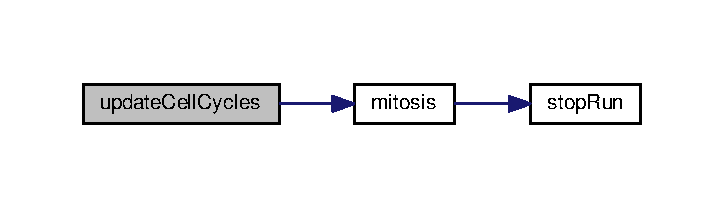
\includegraphics[width=348pt]{cells_8c_a718a88fce87f8ebdb87ed2fafed4c5c4_cgraph}
\end{center}
\end{figure}




Here is the caller graph for this function\-:\nopagebreak
\begin{figure}[H]
\begin{center}
\leavevmode
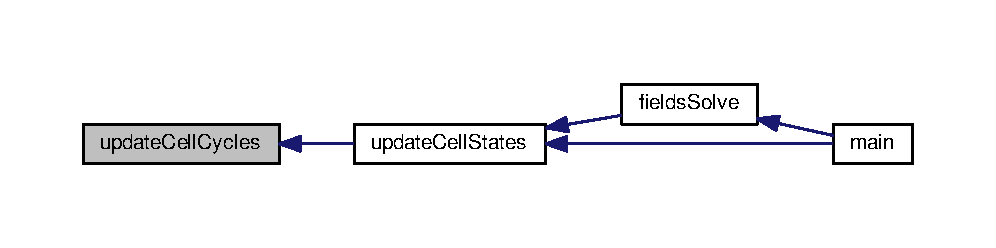
\includegraphics[width=350pt]{cells_8c_a718a88fce87f8ebdb87ed2fafed4c5c4_icgraph}
\end{center}
\end{figure}


\hypertarget{cells_8c_a227256c7da11efa2b4eacedf0a9f37c8}{\index{cells.\-c@{cells.\-c}!update\-Cell\-Positions@{update\-Cell\-Positions}}
\index{update\-Cell\-Positions@{update\-Cell\-Positions}!cells.c@{cells.\-c}}
\subsubsection[{update\-Cell\-Positions}]{\setlength{\rightskip}{0pt plus 5cm}void update\-Cell\-Positions (
\begin{DoxyParamCaption}
{}
\end{DoxyParamCaption}
)}}\label{cells_8c_a227256c7da11efa2b4eacedf0a9f37c8}
This function updates cells' positions. 

Definition at line 504 of file cells.\-c.



References cells, csize, lnc, statistics\-Data\-::mindist, M\-P\-Irank, nc, sim\-Start, statistics, stat\-Out\-Step, step, velocity, cell\-Data\-::x, double\-Vector3d\-::x, cell\-Data\-::y, double\-Vector3d\-::y, cell\-Data\-::z, and double\-Vector3d\-::z.


\begin{DoxyCode}
505 \{
506   \textcolor{keywordtype}{int} c;
507 \textcolor{preprocessor}{#ifdef DEBUG}
508 \textcolor{preprocessor}{}  \textcolor{keywordflow}{if} (\hyperlink{global_8h_a710288ab7d2734acc4566a87a645325d}{MPIrank} == 0 && !(\hyperlink{global_8h_abc16e65f240ed0c8f3e876e8732c0a33}{step} % \hyperlink{global_8h_aab9700fe12cc303ff43e1a35a210128e}{statOutStep})) \{
509     printf(\textcolor{stringliteral}{" Cells movement..."});
510     fflush(stdout);
511   \}
512 \textcolor{preprocessor}{#endif}
513 \textcolor{preprocessor}{}  \textcolor{keywordflow}{if} ((\hyperlink{global_8h_ad9c6b160d2d6fe545e8f9529b237838a}{statistics}.\hyperlink{structstatisticsData_a78455d23ec97258967b76cbb2332b7be}{mindist} >= 0.95 * 2.0 * pow(2.0, -(1.0 / 3.0)) * 
      \hyperlink{global_8h_a3b735e8520f1816ee73ee50daa3ef756}{csize}
514        && \hyperlink{global_8h_a42a935b4eec9242e09d47fc1c2b6dba3}{simStart} == 0) || (\hyperlink{global_8h_a0845b4b004824f1fe3cd69db1672fa15}{nc} == 1 && \hyperlink{global_8h_a42a935b4eec9242e09d47fc1c2b6dba3}{simStart} == 0)) \{
515     \hyperlink{global_8h_a42a935b4eec9242e09d47fc1c2b6dba3}{simStart} = 1;
516     \textcolor{keywordflow}{if} (\hyperlink{global_8h_a710288ab7d2734acc4566a87a645325d}{MPIrank} == 0)
517       printf(\textcolor{stringliteral}{"\(\backslash\)nSimulation started.\(\backslash\)n"});
518   \}
519 
520   \textcolor{comment}{/* move cells */}
521   \textcolor{keywordflow}{for} (c = 0; c < \hyperlink{global_8h_a7065c019590815f10169c219f358e7d0}{lnc}; c++) \{
522     \hyperlink{global_8h_a56da06a03aa369ca203be968cb56d16c}{cells}[c].\hyperlink{structcellData_af88b946fb90d5f08b5fb740c70e98c10}{x} += \hyperlink{global_8h_a6015afb23ea197551ff3d503aa3426a4}{velocity}[c].\hyperlink{structdoubleVector3d_af88b946fb90d5f08b5fb740c70e98c10}{x};
523     \hyperlink{global_8h_a56da06a03aa369ca203be968cb56d16c}{cells}[c].\hyperlink{structcellData_ab927965981178aa1fba979a37168db2a}{y} += \hyperlink{global_8h_a6015afb23ea197551ff3d503aa3426a4}{velocity}[c].\hyperlink{structdoubleVector3d_ab927965981178aa1fba979a37168db2a}{y};
524     \hyperlink{global_8h_a56da06a03aa369ca203be968cb56d16c}{cells}[c].\hyperlink{structcellData_ab3e6ed577a7c669c19de1f9c1b46c872}{z} += \hyperlink{global_8h_a6015afb23ea197551ff3d503aa3426a4}{velocity}[c].\hyperlink{structdoubleVector3d_ab3e6ed577a7c669c19de1f9c1b46c872}{z};
525     \textcolor{comment}{// Mark cells that are out of the box and need to be removed}
526     \textcolor{comment}{//if(outside\_the\_box(c)) \{ celld[c]=1; rsum++; \}}
527   \}
528 \textcolor{preprocessor}{#ifdef DEBUG}
529 \textcolor{preprocessor}{}  \textcolor{keywordflow}{if} (\hyperlink{global_8h_a710288ab7d2734acc4566a87a645325d}{MPIrank} == 0 && !(\hyperlink{global_8h_abc16e65f240ed0c8f3e876e8732c0a33}{step} % statOutStep))
530     printf(\textcolor{stringliteral}{"done\(\backslash\)n"});
531 \textcolor{preprocessor}{#endif}
532 \textcolor{preprocessor}{}\}
\end{DoxyCode}


Here is the caller graph for this function\-:\nopagebreak
\begin{figure}[H]
\begin{center}
\leavevmode
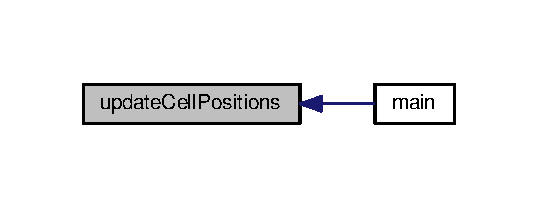
\includegraphics[width=258pt]{cells_8c_a227256c7da11efa2b4eacedf0a9f37c8_icgraph}
\end{center}
\end{figure}


\hypertarget{cells_8c_aeb1f066ef0713a8a50eb1e58784a3d7b}{\index{cells.\-c@{cells.\-c}!update\-Cell\-States@{update\-Cell\-States}}
\index{update\-Cell\-States@{update\-Cell\-States}!cells.c@{cells.\-c}}
\subsubsection[{update\-Cell\-States}]{\setlength{\rightskip}{0pt plus 5cm}void update\-Cell\-States (
\begin{DoxyParamCaption}
{}
\end{DoxyParamCaption}
)}}\label{cells_8c_aeb1f066ef0713a8a50eb1e58784a3d7b}
This function drives the whole cell cycle update. 

Definition at line 718 of file cells.\-c.



References additional\-Scalar\-Field(), cancer, celld, cells\-Death(), lnc, mark\-Middle\-Cancer\-Cell(), nc, nhs, rsum, tgs, update\-Cell\-Counters(), and update\-Cell\-Cycles().


\begin{DoxyCode}
719 \{
720   \textcolor{keywordtype}{int} lnc\_old;
721   \textcolor{comment}{/* number of local cells might change during the update */}
722   lnc\_old = \hyperlink{global_8h_a7065c019590815f10169c219f358e7d0}{lnc};
723   \hyperlink{cells_8c_a96a825c021fe648b7fb171bd2c532ffb}{celld} = (\textcolor{keywordtype}{unsigned} \textcolor{keywordtype}{char} *) calloc(lnc\_old, \textcolor{keyword}{sizeof}(\textcolor{keywordtype}{unsigned} \textcolor{keywordtype}{char}));
724   \hyperlink{global_8h_a087a95bb36c9b36c708a73ce656fd1f1}{rsum} = 0;
725 
726   \hyperlink{cells_8c_a718a88fce87f8ebdb87ed2fafed4c5c4}{updateCellCycles}();
727   \textcolor{keywordflow}{if} (\hyperlink{global_8h_a4c518eee956421a1bf84ad13ab360967}{nhs} > 0 && \hyperlink{global_8h_a0845b4b004824f1fe3cd69db1672fa15}{nc} > \hyperlink{global_8h_a4c518eee956421a1bf84ad13ab360967}{nhs} && \hyperlink{global_8h_ac84ddf735039774c39779789f7afad53}{tgs} == 1 && \hyperlink{global_8h_a543a1902d49aca54ef382bf603a51e27}{cancer} == 0)
728     \hyperlink{cells_8c_a00dbe1f9f23fc7385462c32b89d28cf8}{markMiddleCancerCell}();
729   \textcolor{keywordflow}{if} (\hyperlink{global_8h_a4c518eee956421a1bf84ad13ab360967}{nhs} > 0 && \hyperlink{global_8h_a0845b4b004824f1fe3cd69db1672fa15}{nc} > \hyperlink{global_8h_a4c518eee956421a1bf84ad13ab360967}{nhs})
730     \hyperlink{cells_8c_a8101c456dae07ab9cbd918ccad3a2ff7}{cellsDeath}(lnc\_old);
731   \hyperlink{cells_8c_aeeb6dee9938af6fef987f1c949458703}{updateCellCounters}();
732   \hyperlink{cells_8c_aa2ee543811c23ee4b487102bb71ba9c7}{additionalScalarField}();
733   free(\hyperlink{cells_8c_a96a825c021fe648b7fb171bd2c532ffb}{celld});
734 \}
\end{DoxyCode}


Here is the call graph for this function\-:\nopagebreak
\begin{figure}[H]
\begin{center}
\leavevmode
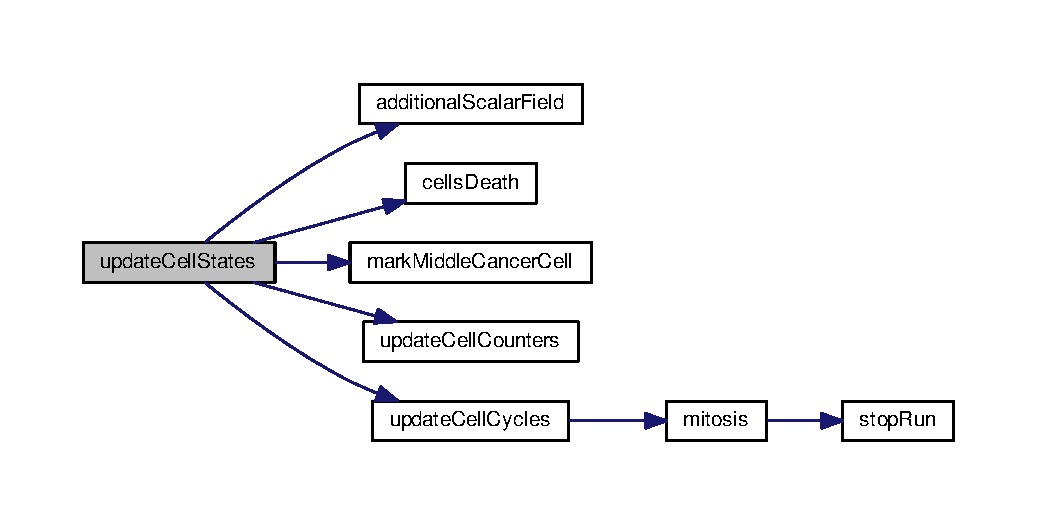
\includegraphics[width=350pt]{cells_8c_aeb1f066ef0713a8a50eb1e58784a3d7b_cgraph}
\end{center}
\end{figure}




Here is the caller graph for this function\-:\nopagebreak
\begin{figure}[H]
\begin{center}
\leavevmode
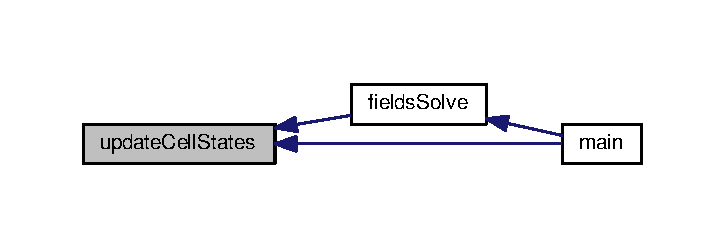
\includegraphics[width=348pt]{cells_8c_aeb1f066ef0713a8a50eb1e58784a3d7b_icgraph}
\end{center}
\end{figure}




\subsection{Variable Documentation}
\hypertarget{cells_8c_a96a825c021fe648b7fb171bd2c532ffb}{\index{cells.\-c@{cells.\-c}!celld@{celld}}
\index{celld@{celld}!cells.c@{cells.\-c}}
\subsubsection[{celld}]{\setlength{\rightskip}{0pt plus 5cm}unsigned char$\ast$ celld}}\label{cells_8c_a96a825c021fe648b7fb171bd2c532ffb}


Definition at line 38 of file cells.\-c.


\hypertarget{chemf_8c}{\section{chemf.\-c File Reference}
\label{chemf_8c}\index{chemf.\-c@{chemf.\-c}}
}


contains functions used for solving chemical global fields  


{\ttfamily \#include $<$float.\-h$>$}\\*
{\ttfamily \#include \char`\"{}\-\_\-hypre\-\_\-utilities.\-h\char`\"{}}\\*
{\ttfamily \#include \char`\"{}H\-Y\-P\-R\-E\-\_\-sstruct\-\_\-ls.\-h\char`\"{}}\\*
{\ttfamily \#include \char`\"{}H\-Y\-P\-R\-E\-\_\-parcsr\-\_\-ls.\-h\char`\"{}}\\*
{\ttfamily \#include \char`\"{}H\-Y\-P\-R\-E\-\_\-krylov.\-h\char`\"{}}\\*
{\ttfamily \#include \char`\"{}global.\-h\char`\"{}}\\*
{\ttfamily \#include \char`\"{}fields.\-h\char`\"{}}\\*
Include dependency graph for chemf.\-c\-:\nopagebreak
\begin{figure}[H]
\begin{center}
\leavevmode
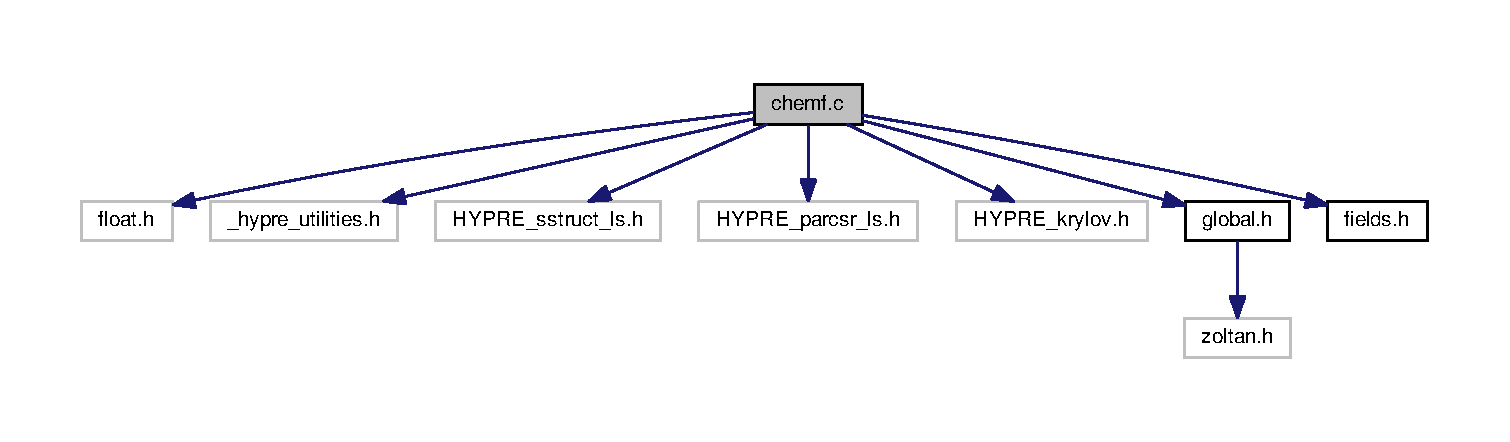
\includegraphics[width=350pt]{chemf_8c__incl}
\end{center}
\end{figure}
\subsection*{Functions}
\begin{DoxyCompactItemize}
\item 
void \hyperlink{chemf_8c_afb692f34ea05262db93f9bf9590b06a7}{chem\-Set\-Boundary} (int coord, int boundary)
\item 
void \hyperlink{chemf_8c_abc9d0a6b17feeff2a62eb6bb38c17ff4}{chem\-Env\-Init\-System} (int nch)
\item 
void \hyperlink{chemf_8c_a5ca738b55b36899ceaa4fe1e6ff38b9f}{chem\-Env\-Cell\-P\-C} (int nch)
\item 
void \hyperlink{chemf_8c_ae67d4d36ecee14805a0b6b0b134b0800}{chem\-Env\-Init\-B\-C} (int nch)
\item 
void \hyperlink{chemf_8c_ad1be1b100191d6ffbd5c3cb0c42549d6}{chem\-Env\-Init\-Solver} (int nch)
\item 
void \hyperlink{chemf_8c_a1f8f7d186d46aafcd792aaf3bee655a7}{chem\-Env\-Solve} (int nch)
\end{DoxyCompactItemize}
\subsection*{Variables}
\begin{DoxyCompactItemize}
\item 
H\-Y\-P\-R\-E\-\_\-\-S\-Struct\-Grid \hyperlink{chemf_8c_ad7a28a5fc279e8b757bdc6a4b57c25be}{chem\-Grid} \mbox{[}\hyperlink{fields_8h_af4afd37668ae33da6377a17adff33029}{N\-C\-H\-E\-M}\mbox{]}
\item 
H\-Y\-P\-R\-E\-\_\-\-S\-Struct\-Graph \hyperlink{chemf_8c_aaac58de32c5dda56ce31654ec3e19337}{chem\-Graph} \mbox{[}\hyperlink{fields_8h_af4afd37668ae33da6377a17adff33029}{N\-C\-H\-E\-M}\mbox{]}
\item 
H\-Y\-P\-R\-E\-\_\-\-S\-Struct\-Stencil \hyperlink{chemf_8c_ae8a36b5c7c6256a7d248a08c71944c73}{chem\-Stencil} \mbox{[}\hyperlink{fields_8h_af4afd37668ae33da6377a17adff33029}{N\-C\-H\-E\-M}\mbox{]}
\item 
H\-Y\-P\-R\-E\-\_\-\-S\-Struct\-Matrix \hyperlink{chemf_8c_ad634e858729e0c04e8b9a4b0a1144b10}{chem\-A} \mbox{[}\hyperlink{fields_8h_af4afd37668ae33da6377a17adff33029}{N\-C\-H\-E\-M}\mbox{]}
\item 
H\-Y\-P\-R\-E\-\_\-\-S\-Struct\-Vector \hyperlink{chemf_8c_afb43e9c9d8160250a03e1b41902473fd}{chemb} \mbox{[}\hyperlink{fields_8h_af4afd37668ae33da6377a17adff33029}{N\-C\-H\-E\-M}\mbox{]}
\item 
H\-Y\-P\-R\-E\-\_\-\-S\-Struct\-Vector \hyperlink{chemf_8c_a48c5bcbe8787c6a6be2a6d5bcdae101f}{chemx} \mbox{[}\hyperlink{fields_8h_af4afd37668ae33da6377a17adff33029}{N\-C\-H\-E\-M}\mbox{]}
\item 
H\-Y\-P\-R\-E\-\_\-\-Par\-C\-S\-R\-Matrix \hyperlink{chemf_8c_a998a7ebb65eb001abcee46c1ea1b1756}{chem\-Par\-A} \mbox{[}\hyperlink{fields_8h_af4afd37668ae33da6377a17adff33029}{N\-C\-H\-E\-M}\mbox{]}
\item 
H\-Y\-P\-R\-E\-\_\-\-Par\-Vector \hyperlink{chemf_8c_af74b7f36ec77fb8e0638db98dd2ee47a}{chem\-Parb} \mbox{[}\hyperlink{fields_8h_af4afd37668ae33da6377a17adff33029}{N\-C\-H\-E\-M}\mbox{]}
\item 
H\-Y\-P\-R\-E\-\_\-\-Par\-Vector \hyperlink{chemf_8c_aae118f98b57f3dda9f036d39db247bb1}{chem\-Parx} \mbox{[}\hyperlink{fields_8h_af4afd37668ae33da6377a17adff33029}{N\-C\-H\-E\-M}\mbox{]}
\item 
H\-Y\-P\-R\-E\-\_\-\-Solver \hyperlink{chemf_8c_a99bbb7b0352d9c850e98287fa45b42c0}{chem\-Solver} \mbox{[}\hyperlink{fields_8h_af4afd37668ae33da6377a17adff33029}{N\-C\-H\-E\-M}\mbox{]}
\item 
H\-Y\-P\-R\-E\-\_\-\-Solver \hyperlink{chemf_8c_a91747632f47bf551e8915e343439777f}{chem\-Precond} \mbox{[}\hyperlink{fields_8h_af4afd37668ae33da6377a17adff33029}{N\-C\-H\-E\-M}\mbox{]}
\item 
int \hyperlink{chemf_8c_a242fb3ba38fb1c6054fd05507394f08b}{chem\-Object\-Type}
\item 
long long \hyperlink{chemf_8c_a14199fec6ea96fe4a4c57bccaff2dfe7}{chem\-Lower} \mbox{[}3\mbox{]}
\item 
long long \hyperlink{chemf_8c_a019f631b2e2795023bf22abef7d9f80e}{chem\-Upper} \mbox{[}3\mbox{]}
\item 
long long \hyperlink{chemf_8c_a397798166a570960b5d468b6df8bf02c}{bc\-Lower} \mbox{[}3\mbox{]}
\item 
long long \hyperlink{chemf_8c_aaea99b8c85fcedb15091dcac991999fd}{bc\-Upper} \mbox{[}3\mbox{]}
\item 
double \hyperlink{chemf_8c_a881c8c944ac83a5c022ee0e236f35e52}{dt} \mbox{[}\hyperlink{fields_8h_af4afd37668ae33da6377a17adff33029}{N\-C\-H\-E\-M}\mbox{]}
\item 
double \hyperlink{chemf_8c_ab35147d777155659aaad43553e3378f4}{chem\-Lambda} = 0.\-25
\item 
char \hyperlink{chemf_8c_a27dc1f70b41e3739d1629663a1d3d0a6}{chfname} \mbox{[}256\mbox{]}
\item 
int \hyperlink{chemf_8c_a26adfe146e722023d7f81bf278bde9e7}{chem\-Iter} \mbox{[}\hyperlink{fields_8h_af4afd37668ae33da6377a17adff33029}{N\-C\-H\-E\-M}\mbox{]}
\item 
double \hyperlink{chemf_8c_ad1178dce1f62833a078c63e911e2e023}{chem\-Z} \mbox{[}\hyperlink{fields_8h_af4afd37668ae33da6377a17adff33029}{N\-C\-H\-E\-M}\mbox{]}
\item 
H\-Y\-P\-R\-E\-\_\-\-S\-Struct\-Variable \hyperlink{chemf_8c_aa73fdbffdd3d43dd503718011b98e41f}{chem\-Vartypes} \mbox{[}1\mbox{]} = \{ H\-Y\-P\-R\-E\-\_\-\-S\-S\-T\-R\-U\-C\-T\-\_\-\-V\-A\-R\-I\-A\-B\-L\-E\-\_\-\-N\-O\-D\-E \}
\item 
int \hyperlink{chemf_8c_a07fef4b421caa5300b13b2ba89422841}{number\-Of\-Iters}
\item 
double $\ast$ \hyperlink{chemf_8c_a614434a804d9a302d1db9603c22b60a7}{chem\-P\-C}
\end{DoxyCompactItemize}


\subsection{Detailed Description}
contains functions used for solving chemical global fields 

Definition in file \hyperlink{chemf_8c_source}{chemf.\-c}.



\subsection{Function Documentation}
\hypertarget{chemf_8c_a5ca738b55b36899ceaa4fe1e6ff38b9f}{\index{chemf.\-c@{chemf.\-c}!chem\-Env\-Cell\-P\-C@{chem\-Env\-Cell\-P\-C}}
\index{chem\-Env\-Cell\-P\-C@{chem\-Env\-Cell\-P\-C}!chemf.c@{chemf.\-c}}
\subsubsection[{chem\-Env\-Cell\-P\-C}]{\setlength{\rightskip}{0pt plus 5cm}void chem\-Env\-Cell\-P\-C (
\begin{DoxyParamCaption}
\item[{int}]{nch}
\end{DoxyParamCaption}
)}}\label{chemf_8c_a5ca738b55b36899ceaa4fe1e6ff38b9f}
This function computes cell production/consumption function based on the interpolated cell density field. 

Definition at line 241 of file chemf.\-c.



References chem\-P\-C, density\-Field, dt, field\-Consumption, field\-Production, grid\-Size, N\-G\-L\-O\-B, step, int64\-Vector3d\-::x, int64\-Vector3d\-::y, and int64\-Vector3d\-::z.


\begin{DoxyCode}
242 \{
243   \textcolor{keywordtype}{int} ch, i, j, k;
244   \textcolor{keywordtype}{long} \textcolor{keywordtype}{long} nvalues = \hyperlink{fields_8h_ae67bb9d09bd0919a0ccbc27b387cec72}{gridSize}.\hyperlink{structint64Vector3d_a040359f45343ce6667f5c66fda5f50e3}{x} * \hyperlink{fields_8h_ae67bb9d09bd0919a0ccbc27b387cec72}{gridSize}.\hyperlink{structint64Vector3d_a0cbcba26311a97b8e0763317e105a918}{y} * \hyperlink{fields_8h_ae67bb9d09bd0919a0ccbc27b387cec72}{gridSize}.
      \hyperlink{structint64Vector3d_a44624880ae3bb63041297b70cb33408b}{z};
245 
246   \textcolor{keywordflow}{if} (\hyperlink{global_8h_abc16e65f240ed0c8f3e876e8732c0a33}{step} == 0)
247     \textcolor{keywordflow}{return};
248 
249   \textcolor{keywordtype}{int} idx = 0;
250   \textcolor{keywordflow}{for} (k = 0; k < \hyperlink{fields_8h_ae67bb9d09bd0919a0ccbc27b387cec72}{gridSize}.\hyperlink{structint64Vector3d_a44624880ae3bb63041297b70cb33408b}{z}; k++)
251     \textcolor{keywordflow}{for} (j = 0; j < \hyperlink{fields_8h_ae67bb9d09bd0919a0ccbc27b387cec72}{gridSize}.\hyperlink{structint64Vector3d_a0cbcba26311a97b8e0763317e105a918}{y}; j++)
252       \textcolor{keywordflow}{for} (i = 0; i < \hyperlink{fields_8h_ae67bb9d09bd0919a0ccbc27b387cec72}{gridSize}.\hyperlink{structint64Vector3d_a040359f45343ce6667f5c66fda5f50e3}{x}; i++, idx++) \{
253     \hyperlink{chemf_8c_a614434a804d9a302d1db9603c22b60a7}{chemPC}[idx] = (-\hyperlink{fields_8h_aa36e8f59ad94c5b7629ce29e6d3edc7e}{fieldConsumption}[nch + \hyperlink{fields_8h_aa40ca56600c708a797a77c1db484958d}{NGLOB}] + 
      \hyperlink{fields_8h_a7bef183ed63be648c7c1f4a63652cb41}{fieldProduction}[nch + \hyperlink{fields_8h_aa40ca56600c708a797a77c1db484958d}{NGLOB}]) * \hyperlink{fields_8h_ab5fe38cf4811c34fa9d1c8e4aa6340c2}{densityField}[
      \hyperlink{fields_8h_ae67bb9d09bd0919a0ccbc27b387cec72}{gridSize}.\hyperlink{structint64Vector3d_a44624880ae3bb63041297b70cb33408b}{z} * \hyperlink{fields_8h_ae67bb9d09bd0919a0ccbc27b387cec72}{gridSize}.\hyperlink{structint64Vector3d_a0cbcba26311a97b8e0763317e105a918}{y} * i + \hyperlink{fields_8h_ae67bb9d09bd0919a0ccbc27b387cec72}{gridSize}.\hyperlink{structint64Vector3d_a44624880ae3bb63041297b70cb33408b}{z} * j + k] * 
      \hyperlink{chemf_8c_a881c8c944ac83a5c022ee0e236f35e52}{dt}[nch];  \textcolor{comment}{//*(cellVolume/boxVolume);//*(1.0/cellVolume);//*dt[nch];//*dt[nch];}
254       \}
255 \}
\end{DoxyCode}


Here is the caller graph for this function\-:\nopagebreak
\begin{figure}[H]
\begin{center}
\leavevmode
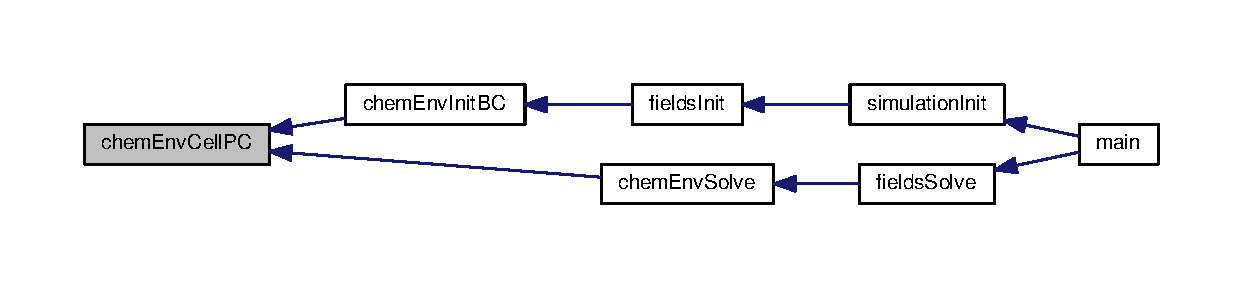
\includegraphics[width=350pt]{chemf_8c_a5ca738b55b36899ceaa4fe1e6ff38b9f_icgraph}
\end{center}
\end{figure}


\hypertarget{chemf_8c_ae67d4d36ecee14805a0b6b0b134b0800}{\index{chemf.\-c@{chemf.\-c}!chem\-Env\-Init\-B\-C@{chem\-Env\-Init\-B\-C}}
\index{chem\-Env\-Init\-B\-C@{chem\-Env\-Init\-B\-C}!chemf.c@{chemf.\-c}}
\subsubsection[{chem\-Env\-Init\-B\-C}]{\setlength{\rightskip}{0pt plus 5cm}void chem\-Env\-Init\-B\-C (
\begin{DoxyParamCaption}
\item[{int}]{nch}
\end{DoxyParamCaption}
)}}\label{chemf_8c_ae67d4d36ecee14805a0b6b0b134b0800}
This function initializes boundary conditions for a given chemical field. 

Definition at line 260 of file chemf.\-c.



References bc\-Lower, bc\-Upper, chem\-A, chemb, chem\-Env\-Cell\-P\-C(), chem\-Grid, chem\-Lower, chem\-Object\-Type, chem\-P\-C, chem\-Set\-Boundary(), chem\-Upper, chemx, chem\-Z, chfname, field\-B\-C, field\-I\-C\-Mean, grid\-Size, m, M\-P\-I\-\_\-\-C\-A\-R\-T\-\_\-\-C\-O\-M\-M, M\-P\-Icoords, M\-P\-Idim, M\-P\-Irank, N\-G\-L\-O\-B, revert\-Std\-Out(), switch\-Std\-Out(), int64\-Vector3d\-::x, int64\-Vector3d\-::y, and int64\-Vector3d\-::z.


\begin{DoxyCode}
261 \{
262   \textcolor{keywordtype}{int} i, j, k;
263   \textcolor{keywordtype}{int} \hyperlink{global_8h_ac51334f57ef8b81c0629c9421798c344}{m};
264   \textcolor{keywordtype}{int} nentries = 1;
265   \textcolor{keywordtype}{long} \textcolor{keywordtype}{long} stencil\_indices[1];
266   \textcolor{keywordtype}{long} \textcolor{keywordtype}{long} nvalues = \hyperlink{fields_8h_ae67bb9d09bd0919a0ccbc27b387cec72}{gridSize}.\hyperlink{structint64Vector3d_a040359f45343ce6667f5c66fda5f50e3}{x} * \hyperlink{fields_8h_ae67bb9d09bd0919a0ccbc27b387cec72}{gridSize}.\hyperlink{structint64Vector3d_a0cbcba26311a97b8e0763317e105a918}{y} * \hyperlink{fields_8h_ae67bb9d09bd0919a0ccbc27b387cec72}{gridSize}.
      \hyperlink{structint64Vector3d_a44624880ae3bb63041297b70cb33408b}{z};
267   \textcolor{keywordtype}{double} *values, *bvalues;
268   \textcolor{comment}{/* stdout redirected to file */}
269   \hyperlink{io_8c_a62f5074e9f833de4cbf65a82dbb2f81b}{switchStdOut}(\hyperlink{chemf_8c_a27dc1f70b41e3739d1629663a1d3d0a6}{chfname});
270 
271   \hyperlink{chemf_8c_a614434a804d9a302d1db9603c22b60a7}{chemPC} = (\textcolor{keywordtype}{double} *) calloc(nvalues, \textcolor{keyword}{sizeof}(\textcolor{keywordtype}{double}));
272   values = calloc(nvalues, \textcolor{keyword}{sizeof}(\textcolor{keywordtype}{double}));
273   bvalues = calloc(nvalues, \textcolor{keyword}{sizeof}(\textcolor{keywordtype}{double}));
274 
275   \hyperlink{chemf_8c_a5ca738b55b36899ceaa4fe1e6ff38b9f}{chemEnvCellPC}(nch);
276 
277   \textcolor{comment}{/* 5. SETUP STRUCT VECTORS FOR B AND X */}
278 
279   \textcolor{comment}{/* create an empty vector object */}
280   HYPRE\_SStructVectorCreate(\hyperlink{global_8h_a34ac355617a6a906e1f3e7832aeb0073}{MPI\_CART\_COMM}, \hyperlink{chemf_8c_ad7a28a5fc279e8b757bdc6a4b57c25be}{chemGrid}[nch], &
      \hyperlink{chemf_8c_afb43e9c9d8160250a03e1b41902473fd}{chemb}[nch]);
281   HYPRE\_SStructVectorCreate(\hyperlink{global_8h_a34ac355617a6a906e1f3e7832aeb0073}{MPI\_CART\_COMM}, \hyperlink{chemf_8c_ad7a28a5fc279e8b757bdc6a4b57c25be}{chemGrid}[nch], &
      \hyperlink{chemf_8c_a48c5bcbe8787c6a6be2a6d5bcdae101f}{chemx}[nch]);
282 
283   \textcolor{comment}{/* as with the matrix, set the appropriate object type for the vectors */}
284   HYPRE\_SStructVectorSetObjectType(\hyperlink{chemf_8c_afb43e9c9d8160250a03e1b41902473fd}{chemb}[nch], \hyperlink{chemf_8c_a242fb3ba38fb1c6054fd05507394f08b}{chemObjectType});
285   HYPRE\_SStructVectorSetObjectType(\hyperlink{chemf_8c_a48c5bcbe8787c6a6be2a6d5bcdae101f}{chemx}[nch], \hyperlink{chemf_8c_a242fb3ba38fb1c6054fd05507394f08b}{chemObjectType});
286 
287   \textcolor{comment}{/* indicate that the vector coefficients are ready to be set */}
288   HYPRE\_SStructVectorInitialize(\hyperlink{chemf_8c_afb43e9c9d8160250a03e1b41902473fd}{chemb}[nch]);
289   HYPRE\_SStructVectorInitialize(\hyperlink{chemf_8c_a48c5bcbe8787c6a6be2a6d5bcdae101f}{chemx}[nch]);
290 
291   \textcolor{comment}{/* set the values */}
292   m = 0;
293   \textcolor{keywordflow}{for} (k = \hyperlink{chemf_8c_a14199fec6ea96fe4a4c57bccaff2dfe7}{chemLower}[2]; k <= \hyperlink{chemf_8c_a019f631b2e2795023bf22abef7d9f80e}{chemUpper}[2]; k++)
294     \textcolor{keywordflow}{for} (j = \hyperlink{chemf_8c_a14199fec6ea96fe4a4c57bccaff2dfe7}{chemLower}[1]; j <= \hyperlink{chemf_8c_a019f631b2e2795023bf22abef7d9f80e}{chemUpper}[1]; j++)
295       \textcolor{keywordflow}{for} (i = \hyperlink{chemf_8c_a14199fec6ea96fe4a4c57bccaff2dfe7}{chemLower}[0]; i <= \hyperlink{chemf_8c_a019f631b2e2795023bf22abef7d9f80e}{chemUpper}[0]; i++) \{
296     values[\hyperlink{global_8h_ac51334f57ef8b81c0629c9421798c344}{m}] = \hyperlink{fields_8h_ad0fb86debb3e1b138683ff94a2f51f5b}{fieldICMean}[nch + \hyperlink{fields_8h_aa40ca56600c708a797a77c1db484958d}{NGLOB}];
297     m++;
298       \}
299 
300   HYPRE\_SStructVectorSetBoxValues(\hyperlink{chemf_8c_afb43e9c9d8160250a03e1b41902473fd}{chemb}[nch], 0, \hyperlink{chemf_8c_a14199fec6ea96fe4a4c57bccaff2dfe7}{chemLower}, 
      \hyperlink{chemf_8c_a019f631b2e2795023bf22abef7d9f80e}{chemUpper}, 0,
301                   values);
302 
303   m = 0;
304   \textcolor{keywordflow}{for} (k = \hyperlink{chemf_8c_a14199fec6ea96fe4a4c57bccaff2dfe7}{chemLower}[2]; k <= \hyperlink{chemf_8c_a019f631b2e2795023bf22abef7d9f80e}{chemUpper}[2]; k++)
305     \textcolor{keywordflow}{for} (j = \hyperlink{chemf_8c_a14199fec6ea96fe4a4c57bccaff2dfe7}{chemLower}[1]; j <= \hyperlink{chemf_8c_a019f631b2e2795023bf22abef7d9f80e}{chemUpper}[1]; j++)
306       \textcolor{keywordflow}{for} (i = \hyperlink{chemf_8c_a14199fec6ea96fe4a4c57bccaff2dfe7}{chemLower}[0]; i <= \hyperlink{chemf_8c_a019f631b2e2795023bf22abef7d9f80e}{chemUpper}[0]; i++) \{
307     values[\hyperlink{global_8h_ac51334f57ef8b81c0629c9421798c344}{m}] = \hyperlink{fields_8h_ad0fb86debb3e1b138683ff94a2f51f5b}{fieldICMean}[nch + \hyperlink{fields_8h_aa40ca56600c708a797a77c1db484958d}{NGLOB}];
308     m++;
309       \}
310 
311   HYPRE\_SStructVectorSetBoxValues(\hyperlink{chemf_8c_a48c5bcbe8787c6a6be2a6d5bcdae101f}{chemx}[nch], 0, \hyperlink{chemf_8c_a14199fec6ea96fe4a4c57bccaff2dfe7}{chemLower}, 
      \hyperlink{chemf_8c_a019f631b2e2795023bf22abef7d9f80e}{chemUpper}, 0,
312                   values);
313 
314   \textcolor{comment}{/* incorporate boundary conditions; Dirichlet on 6 faces */}
315 
316   \textcolor{keywordflow}{for} (i = 0; i < nvalues; i++)
317     values[i] = \hyperlink{chemf_8c_ad1178dce1f62833a078c63e911e2e023}{chemZ}[nch];
318   \textcolor{keywordflow}{for} (i = 0; i < nvalues; i++)
319     bvalues[i] = \hyperlink{chemf_8c_ad1178dce1f62833a078c63e911e2e023}{chemZ}[nch] * \hyperlink{fields_8h_a80c6ee80e0f056adba2430ab0d21e58f}{fieldBC}[nch + \hyperlink{fields_8h_aa40ca56600c708a797a77c1db484958d}{NGLOB}];
320 
321   \textcolor{keywordflow}{if} (\hyperlink{global_8h_a8220294108e39b58632993a50a7dc4ca}{MPIcoords}[\hyperlink{global_8h_a710288ab7d2734acc4566a87a645325d}{MPIrank}][0] == 0) \{
322     nvalues = nentries * \hyperlink{fields_8h_ae67bb9d09bd0919a0ccbc27b387cec72}{gridSize}.\hyperlink{structint64Vector3d_a0cbcba26311a97b8e0763317e105a918}{y} * \hyperlink{fields_8h_ae67bb9d09bd0919a0ccbc27b387cec72}{gridSize}.\hyperlink{structint64Vector3d_a44624880ae3bb63041297b70cb33408b}{z};
323     \hyperlink{chemf_8c_afb692f34ea05262db93f9bf9590b06a7}{chemSetBoundary}(0, -1);
324     stencil\_indices[0] = 1;
325     HYPRE\_SStructMatrixAddToBoxValues(\hyperlink{chemf_8c_ad634e858729e0c04e8b9a4b0a1144b10}{chemA}[nch], 0, \hyperlink{chemf_8c_a397798166a570960b5d468b6df8bf02c}{bcLower}, 
      \hyperlink{chemf_8c_aaea99b8c85fcedb15091dcac991999fd}{bcUpper}, 0,
326                       nentries, stencil\_indices, values);
327     HYPRE\_SStructVectorAddToBoxValues(\hyperlink{chemf_8c_afb43e9c9d8160250a03e1b41902473fd}{chemb}[nch], 0, \hyperlink{chemf_8c_a397798166a570960b5d468b6df8bf02c}{bcLower}, 
      \hyperlink{chemf_8c_aaea99b8c85fcedb15091dcac991999fd}{bcUpper}, 0,
328                       bvalues);
329   \}
330   \textcolor{keywordflow}{if} (\hyperlink{global_8h_a8220294108e39b58632993a50a7dc4ca}{MPIcoords}[\hyperlink{global_8h_a710288ab7d2734acc4566a87a645325d}{MPIrank}][0] == \hyperlink{global_8h_a633835398408aaee46fd56809af73e6c}{MPIdim}[0] - 1) \{
331     nvalues = nentries * \hyperlink{fields_8h_ae67bb9d09bd0919a0ccbc27b387cec72}{gridSize}.\hyperlink{structint64Vector3d_a0cbcba26311a97b8e0763317e105a918}{y} * \hyperlink{fields_8h_ae67bb9d09bd0919a0ccbc27b387cec72}{gridSize}.\hyperlink{structint64Vector3d_a44624880ae3bb63041297b70cb33408b}{z};
332     \hyperlink{chemf_8c_afb692f34ea05262db93f9bf9590b06a7}{chemSetBoundary}(0, 1);
333     stencil\_indices[0] = 2;
334     HYPRE\_SStructMatrixAddToBoxValues(\hyperlink{chemf_8c_ad634e858729e0c04e8b9a4b0a1144b10}{chemA}[nch], 0, \hyperlink{chemf_8c_a397798166a570960b5d468b6df8bf02c}{bcLower}, 
      \hyperlink{chemf_8c_aaea99b8c85fcedb15091dcac991999fd}{bcUpper}, 0,
335                       nentries, stencil\_indices, values);
336     HYPRE\_SStructVectorAddToBoxValues(\hyperlink{chemf_8c_afb43e9c9d8160250a03e1b41902473fd}{chemb}[nch], 0, \hyperlink{chemf_8c_a397798166a570960b5d468b6df8bf02c}{bcLower}, 
      \hyperlink{chemf_8c_aaea99b8c85fcedb15091dcac991999fd}{bcUpper}, 0,
337                       bvalues);
338   \}
339   \textcolor{keywordflow}{if} (\hyperlink{global_8h_a8220294108e39b58632993a50a7dc4ca}{MPIcoords}[\hyperlink{global_8h_a710288ab7d2734acc4566a87a645325d}{MPIrank}][1] == 0) \{
340     nvalues = nentries * \hyperlink{fields_8h_ae67bb9d09bd0919a0ccbc27b387cec72}{gridSize}.\hyperlink{structint64Vector3d_a040359f45343ce6667f5c66fda5f50e3}{x} * \hyperlink{fields_8h_ae67bb9d09bd0919a0ccbc27b387cec72}{gridSize}.\hyperlink{structint64Vector3d_a44624880ae3bb63041297b70cb33408b}{z};
341     \hyperlink{chemf_8c_afb692f34ea05262db93f9bf9590b06a7}{chemSetBoundary}(1, -1);
342     stencil\_indices[0] = 3;
343     HYPRE\_SStructMatrixAddToBoxValues(\hyperlink{chemf_8c_ad634e858729e0c04e8b9a4b0a1144b10}{chemA}[nch], 0, \hyperlink{chemf_8c_a397798166a570960b5d468b6df8bf02c}{bcLower}, 
      \hyperlink{chemf_8c_aaea99b8c85fcedb15091dcac991999fd}{bcUpper}, 0,
344                       nentries, stencil\_indices, values);
345     HYPRE\_SStructVectorAddToBoxValues(\hyperlink{chemf_8c_afb43e9c9d8160250a03e1b41902473fd}{chemb}[nch], 0, \hyperlink{chemf_8c_a397798166a570960b5d468b6df8bf02c}{bcLower}, 
      \hyperlink{chemf_8c_aaea99b8c85fcedb15091dcac991999fd}{bcUpper}, 0,
346                       bvalues);
347   \}
348   \textcolor{keywordflow}{if} (\hyperlink{global_8h_a8220294108e39b58632993a50a7dc4ca}{MPIcoords}[\hyperlink{global_8h_a710288ab7d2734acc4566a87a645325d}{MPIrank}][1] == \hyperlink{global_8h_a633835398408aaee46fd56809af73e6c}{MPIdim}[1] - 1) \{
349     nvalues = nentries * \hyperlink{fields_8h_ae67bb9d09bd0919a0ccbc27b387cec72}{gridSize}.\hyperlink{structint64Vector3d_a040359f45343ce6667f5c66fda5f50e3}{x} * \hyperlink{fields_8h_ae67bb9d09bd0919a0ccbc27b387cec72}{gridSize}.\hyperlink{structint64Vector3d_a44624880ae3bb63041297b70cb33408b}{z};
350     \hyperlink{chemf_8c_afb692f34ea05262db93f9bf9590b06a7}{chemSetBoundary}(1, 1);
351     stencil\_indices[0] = 4;
352     HYPRE\_SStructMatrixAddToBoxValues(\hyperlink{chemf_8c_ad634e858729e0c04e8b9a4b0a1144b10}{chemA}[nch], 0, \hyperlink{chemf_8c_a397798166a570960b5d468b6df8bf02c}{bcLower}, 
      \hyperlink{chemf_8c_aaea99b8c85fcedb15091dcac991999fd}{bcUpper}, 0,
353                       nentries, stencil\_indices, values);
354     HYPRE\_SStructVectorAddToBoxValues(\hyperlink{chemf_8c_afb43e9c9d8160250a03e1b41902473fd}{chemb}[nch], 0, \hyperlink{chemf_8c_a397798166a570960b5d468b6df8bf02c}{bcLower}, 
      \hyperlink{chemf_8c_aaea99b8c85fcedb15091dcac991999fd}{bcUpper}, 0,
355                       bvalues);
356   \}
357   \textcolor{keywordflow}{if} (\hyperlink{global_8h_a8220294108e39b58632993a50a7dc4ca}{MPIcoords}[\hyperlink{global_8h_a710288ab7d2734acc4566a87a645325d}{MPIrank}][2] == 0) \{
358     nvalues = nentries * \hyperlink{fields_8h_ae67bb9d09bd0919a0ccbc27b387cec72}{gridSize}.\hyperlink{structint64Vector3d_a040359f45343ce6667f5c66fda5f50e3}{x} * \hyperlink{fields_8h_ae67bb9d09bd0919a0ccbc27b387cec72}{gridSize}.\hyperlink{structint64Vector3d_a0cbcba26311a97b8e0763317e105a918}{y};
359     \hyperlink{chemf_8c_afb692f34ea05262db93f9bf9590b06a7}{chemSetBoundary}(2, -1);
360     stencil\_indices[0] = 5;
361     HYPRE\_SStructMatrixAddToBoxValues(\hyperlink{chemf_8c_ad634e858729e0c04e8b9a4b0a1144b10}{chemA}[nch], 0, \hyperlink{chemf_8c_a397798166a570960b5d468b6df8bf02c}{bcLower}, 
      \hyperlink{chemf_8c_aaea99b8c85fcedb15091dcac991999fd}{bcUpper}, 0,
362                       nentries, stencil\_indices, values);
363     HYPRE\_SStructVectorAddToBoxValues(\hyperlink{chemf_8c_afb43e9c9d8160250a03e1b41902473fd}{chemb}[nch], 0, \hyperlink{chemf_8c_a397798166a570960b5d468b6df8bf02c}{bcLower}, 
      \hyperlink{chemf_8c_aaea99b8c85fcedb15091dcac991999fd}{bcUpper}, 0,
364                       bvalues);
365   \}
366   \textcolor{keywordflow}{if} (\hyperlink{global_8h_a8220294108e39b58632993a50a7dc4ca}{MPIcoords}[\hyperlink{global_8h_a710288ab7d2734acc4566a87a645325d}{MPIrank}][2] == \hyperlink{global_8h_a633835398408aaee46fd56809af73e6c}{MPIdim}[2] - 1) \{
367     nvalues = nentries * \hyperlink{fields_8h_ae67bb9d09bd0919a0ccbc27b387cec72}{gridSize}.\hyperlink{structint64Vector3d_a040359f45343ce6667f5c66fda5f50e3}{x} * \hyperlink{fields_8h_ae67bb9d09bd0919a0ccbc27b387cec72}{gridSize}.\hyperlink{structint64Vector3d_a0cbcba26311a97b8e0763317e105a918}{y};
368     \hyperlink{chemf_8c_afb692f34ea05262db93f9bf9590b06a7}{chemSetBoundary}(2, 1);
369     stencil\_indices[0] = 6;
370     HYPRE\_SStructMatrixAddToBoxValues(\hyperlink{chemf_8c_ad634e858729e0c04e8b9a4b0a1144b10}{chemA}[nch], 0, \hyperlink{chemf_8c_a397798166a570960b5d468b6df8bf02c}{bcLower}, 
      \hyperlink{chemf_8c_aaea99b8c85fcedb15091dcac991999fd}{bcUpper}, 0,
371                       nentries, stencil\_indices, values);
372     HYPRE\_SStructVectorAddToBoxValues(\hyperlink{chemf_8c_afb43e9c9d8160250a03e1b41902473fd}{chemb}[nch], 0, \hyperlink{chemf_8c_a397798166a570960b5d468b6df8bf02c}{bcLower}, 
      \hyperlink{chemf_8c_aaea99b8c85fcedb15091dcac991999fd}{bcUpper}, 0,
373                       bvalues);
374   \}
375 
376   \textcolor{comment}{/* add production consumption function to the right side */}
377   HYPRE\_SStructVectorAddToBoxValues(\hyperlink{chemf_8c_afb43e9c9d8160250a03e1b41902473fd}{chemb}[nch], 0, \hyperlink{chemf_8c_a14199fec6ea96fe4a4c57bccaff2dfe7}{chemLower}, 
      \hyperlink{chemf_8c_a019f631b2e2795023bf22abef7d9f80e}{chemUpper}, 0,
378                     \hyperlink{chemf_8c_a614434a804d9a302d1db9603c22b60a7}{chemPC});
379 
380   free(\hyperlink{chemf_8c_a614434a804d9a302d1db9603c22b60a7}{chemPC});
381   free(values);
382   free(bvalues);
383   \textcolor{comment}{/* stdout brought back */}
384   \hyperlink{io_8c_affa00173da9bea48973a6ac887d505bb}{revertStdOut}();
385 \}
\end{DoxyCode}


Here is the call graph for this function\-:\nopagebreak
\begin{figure}[H]
\begin{center}
\leavevmode
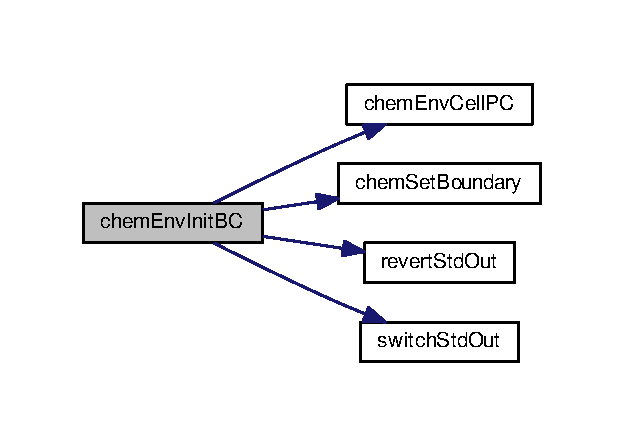
\includegraphics[width=300pt]{chemf_8c_ae67d4d36ecee14805a0b6b0b134b0800_cgraph}
\end{center}
\end{figure}




Here is the caller graph for this function\-:\nopagebreak
\begin{figure}[H]
\begin{center}
\leavevmode
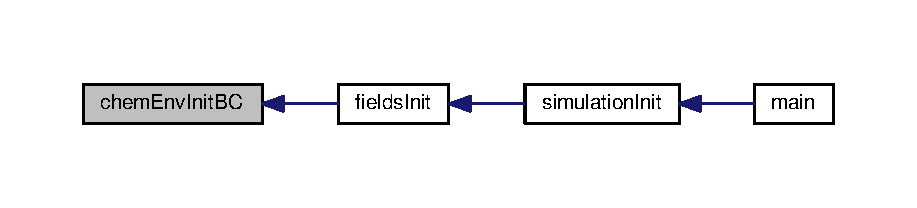
\includegraphics[width=350pt]{chemf_8c_ae67d4d36ecee14805a0b6b0b134b0800_icgraph}
\end{center}
\end{figure}


\hypertarget{chemf_8c_ad1be1b100191d6ffbd5c3cb0c42549d6}{\index{chemf.\-c@{chemf.\-c}!chem\-Env\-Init\-Solver@{chem\-Env\-Init\-Solver}}
\index{chem\-Env\-Init\-Solver@{chem\-Env\-Init\-Solver}!chemf.c@{chemf.\-c}}
\subsubsection[{chem\-Env\-Init\-Solver}]{\setlength{\rightskip}{0pt plus 5cm}void chem\-Env\-Init\-Solver (
\begin{DoxyParamCaption}
\item[{int}]{nch}
\end{DoxyParamCaption}
)}}\label{chemf_8c_ad1be1b100191d6ffbd5c3cb0c42549d6}
This function initializes Hypre for solving a given chemical field. 

Definition at line 390 of file chemf.\-c.



References chem\-A, chemb, chem\-Par\-A, chem\-Parb, chem\-Parx, chem\-Precond, chem\-Solver, chemx, chfname, M\-P\-I\-\_\-\-C\-A\-R\-T\-\_\-\-C\-O\-M\-M, revert\-Std\-Out(), and switch\-Std\-Out().


\begin{DoxyCode}
391 \{
392   \textcolor{comment}{/* stdout redirected to file */}
393   \hyperlink{io_8c_a62f5074e9f833de4cbf65a82dbb2f81b}{switchStdOut}(\hyperlink{chemf_8c_a27dc1f70b41e3739d1629663a1d3d0a6}{chfname});
394 
395   HYPRE\_SStructMatrixAssemble(\hyperlink{chemf_8c_ad634e858729e0c04e8b9a4b0a1144b10}{chemA}[nch]);
396   \textcolor{comment}{/* This is a collective call finalizing the vector assembly.}
397 \textcolor{comment}{     The vector is now ``ready to be used'' */}
398   HYPRE\_SStructVectorAssemble(\hyperlink{chemf_8c_afb43e9c9d8160250a03e1b41902473fd}{chemb}[nch]);
399   HYPRE\_SStructVectorAssemble(\hyperlink{chemf_8c_a48c5bcbe8787c6a6be2a6d5bcdae101f}{chemx}[nch]);
400 
401   HYPRE\_SStructMatrixGetObject(\hyperlink{chemf_8c_ad634e858729e0c04e8b9a4b0a1144b10}{chemA}[nch], (\textcolor{keywordtype}{void} **) &\hyperlink{chemf_8c_a998a7ebb65eb001abcee46c1ea1b1756}{chemParA}[nch]);
402   HYPRE\_SStructVectorGetObject(\hyperlink{chemf_8c_afb43e9c9d8160250a03e1b41902473fd}{chemb}[nch], (\textcolor{keywordtype}{void} **) &\hyperlink{chemf_8c_af74b7f36ec77fb8e0638db98dd2ee47a}{chemParb}[nch]);
403   HYPRE\_SStructVectorGetObject(\hyperlink{chemf_8c_a48c5bcbe8787c6a6be2a6d5bcdae101f}{chemx}[nch], (\textcolor{keywordtype}{void} **) &\hyperlink{chemf_8c_aae118f98b57f3dda9f036d39db247bb1}{chemParx}[nch]);
404 
405   HYPRE\_ParCSRPCGCreate(\hyperlink{global_8h_a34ac355617a6a906e1f3e7832aeb0073}{MPI\_CART\_COMM}, &\hyperlink{chemf_8c_a99bbb7b0352d9c850e98287fa45b42c0}{chemSolver}[nch]);
406   HYPRE\_ParCSRPCGSetTol(\hyperlink{chemf_8c_a99bbb7b0352d9c850e98287fa45b42c0}{chemSolver}[nch], 1.0e-12);
407   HYPRE\_ParCSRPCGSetPrintLevel(\hyperlink{chemf_8c_a99bbb7b0352d9c850e98287fa45b42c0}{chemSolver}[nch], 2);
408   HYPRE\_ParCSRPCGSetMaxIter(\hyperlink{chemf_8c_a99bbb7b0352d9c850e98287fa45b42c0}{chemSolver}[nch], 50);
409 
410   HYPRE\_BoomerAMGCreate(&\hyperlink{chemf_8c_a91747632f47bf551e8915e343439777f}{chemPrecond}[nch]);
411   HYPRE\_BoomerAMGSetMaxIter(\hyperlink{chemf_8c_a91747632f47bf551e8915e343439777f}{chemPrecond}[nch], 1);
412   HYPRE\_BoomerAMGSetTol(\hyperlink{chemf_8c_a91747632f47bf551e8915e343439777f}{chemPrecond}[nch], 0.0);
413   HYPRE\_BoomerAMGSetPrintLevel(\hyperlink{chemf_8c_a91747632f47bf551e8915e343439777f}{chemPrecond}[nch], 2);
414   HYPRE\_BoomerAMGSetCoarsenType(\hyperlink{chemf_8c_a91747632f47bf551e8915e343439777f}{chemPrecond}[nch], 6);
415   HYPRE\_BoomerAMGSetRelaxType(\hyperlink{chemf_8c_a91747632f47bf551e8915e343439777f}{chemPrecond}[nch], 6);
416   HYPRE\_BoomerAMGSetNumSweeps(\hyperlink{chemf_8c_a91747632f47bf551e8915e343439777f}{chemPrecond}[nch], 1);
417 
418   HYPRE\_ParCSRPCGSetPrecond(\hyperlink{chemf_8c_a99bbb7b0352d9c850e98287fa45b42c0}{chemSolver}[nch], HYPRE\_BoomerAMGSolve,
419                 HYPRE\_BoomerAMGSetup, \hyperlink{chemf_8c_a91747632f47bf551e8915e343439777f}{chemPrecond}[nch]);
420   HYPRE\_ParCSRPCGSetup(\hyperlink{chemf_8c_a99bbb7b0352d9c850e98287fa45b42c0}{chemSolver}[nch], \hyperlink{chemf_8c_a998a7ebb65eb001abcee46c1ea1b1756}{chemParA}[nch], 
      \hyperlink{chemf_8c_af74b7f36ec77fb8e0638db98dd2ee47a}{chemParb}[nch],
421                \hyperlink{chemf_8c_aae118f98b57f3dda9f036d39db247bb1}{chemParx}[nch]);
422 
423   \textcolor{comment}{/* stdout brought back */}
424   \hyperlink{io_8c_affa00173da9bea48973a6ac887d505bb}{revertStdOut}();
425 \}
\end{DoxyCode}


Here is the call graph for this function\-:\nopagebreak
\begin{figure}[H]
\begin{center}
\leavevmode
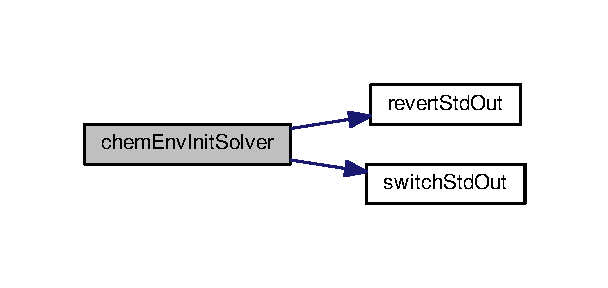
\includegraphics[width=292pt]{chemf_8c_ad1be1b100191d6ffbd5c3cb0c42549d6_cgraph}
\end{center}
\end{figure}




Here is the caller graph for this function\-:\nopagebreak
\begin{figure}[H]
\begin{center}
\leavevmode
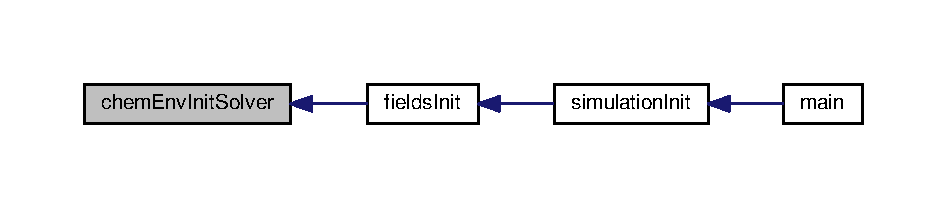
\includegraphics[width=350pt]{chemf_8c_ad1be1b100191d6ffbd5c3cb0c42549d6_icgraph}
\end{center}
\end{figure}


\hypertarget{chemf_8c_abc9d0a6b17feeff2a62eb6bb38c17ff4}{\index{chemf.\-c@{chemf.\-c}!chem\-Env\-Init\-System@{chem\-Env\-Init\-System}}
\index{chem\-Env\-Init\-System@{chem\-Env\-Init\-System}!chemf.c@{chemf.\-c}}
\subsubsection[{chem\-Env\-Init\-System}]{\setlength{\rightskip}{0pt plus 5cm}void chem\-Env\-Init\-System (
\begin{DoxyParamCaption}
\item[{int}]{nch}
\end{DoxyParamCaption}
)}}\label{chemf_8c_abc9d0a6b17feeff2a62eb6bb38c17ff4}
This function initializes grid, stencil and matrix for a given chemical field. 

Definition at line 130 of file chemf.\-c.



References cell\-Fields, chem\-A, chem\-Field, chem\-Graph, chem\-Grid, chem\-Iter, chem\-Lower, chem\-Object\-Type, chem\-Stencil, chem\-Upper, chem\-Vartypes, chem\-Z, chfname, csize, csize\-In\-Units, dt, field\-Diff\-Coef, field\-Dt, field\-I\-C\-Mean, field\-Lambda, field\-Max, field\-Min, grid\-End\-Idx, grid\-Resolution, grid\-Size, grid\-Start\-Idx, logdir, max\-Cells\-Per\-Proc, M\-P\-I\-\_\-\-C\-A\-R\-T\-\_\-\-C\-O\-M\-M, M\-P\-Irank, N\-G\-L\-O\-B, number\-Of\-Iters, revert\-Std\-Out(), switch\-Std\-Out(), int64\-Vector3d\-::x, int64\-Vector3d\-::y, and int64\-Vector3d\-::z.


\begin{DoxyCode}
131 \{
132   \textcolor{keywordtype}{int} i, j, k, c;
133   \textcolor{keywordtype}{int} entry;
134   \textcolor{keywordtype}{long} \textcolor{keywordtype}{long} offsets[7][3] =
135       \{ \{0, 0, 0\}, \{-1, 0, 0\}, \{1, 0, 0\}, \{0, -1, 0\}, \{0, 1, 0\}, \{0, 0,
136                                   -1\}, \{0,
137                                     0,
138                                     1\}
139   \};
140   \textcolor{keywordtype}{double} gridResolutionInUnits; \textcolor{comment}{/* grid resolution in centimeters */}
141 
142   \hyperlink{chemf_8c_a881c8c944ac83a5c022ee0e236f35e52}{dt}[nch] = \hyperlink{fields_8h_ae21d99cc23aefdfc02fbe62cd28784fb}{fieldDt}[nch + \hyperlink{fields_8h_aa40ca56600c708a797a77c1db484958d}{NGLOB}];
143   \hyperlink{chemf_8c_a07fef4b421caa5300b13b2ba89422841}{numberOfIters} = 1;
144   \hyperlink{chemf_8c_a26adfe146e722023d7f81bf278bde9e7}{chemIter}[nch] = 0;
145 
146   sprintf(\hyperlink{chemf_8c_a27dc1f70b41e3739d1629663a1d3d0a6}{chfname}, \textcolor{stringliteral}{"%s/chemSolver.log"}, \hyperlink{global_8h_a58bd7d9996cba89c834ae9ec41bbc075}{logdir});
147   \textcolor{comment}{/* stdout will go to the file */}
148   \hyperlink{io_8c_a62f5074e9f833de4cbf65a82dbb2f81b}{switchStdOut}(\hyperlink{chemf_8c_a27dc1f70b41e3739d1629663a1d3d0a6}{chfname});
149 
150   \textcolor{comment}{/* 1. INIT GRID */}
151 
152   \textcolor{comment}{/* create an empty 3D grid object */}
153   HYPRE\_SStructGridCreate(\hyperlink{global_8h_a34ac355617a6a906e1f3e7832aeb0073}{MPI\_CART\_COMM}, 3, 1, &\hyperlink{chemf_8c_ad7a28a5fc279e8b757bdc6a4b57c25be}{chemGrid}[nch]);
154 
155   \textcolor{comment}{/* set this process box */}
156   \hyperlink{chemf_8c_a14199fec6ea96fe4a4c57bccaff2dfe7}{chemLower}[0] = \hyperlink{fields_8h_a9154f33f7786c05c61f4d519da14d501}{gridStartIdx}[\hyperlink{global_8h_a710288ab7d2734acc4566a87a645325d}{MPIrank}].\hyperlink{structint64Vector3d_a040359f45343ce6667f5c66fda5f50e3}{x};
157   \hyperlink{chemf_8c_a14199fec6ea96fe4a4c57bccaff2dfe7}{chemLower}[1] = \hyperlink{fields_8h_a9154f33f7786c05c61f4d519da14d501}{gridStartIdx}[\hyperlink{global_8h_a710288ab7d2734acc4566a87a645325d}{MPIrank}].\hyperlink{structint64Vector3d_a0cbcba26311a97b8e0763317e105a918}{y};
158   \hyperlink{chemf_8c_a14199fec6ea96fe4a4c57bccaff2dfe7}{chemLower}[2] = \hyperlink{fields_8h_a9154f33f7786c05c61f4d519da14d501}{gridStartIdx}[\hyperlink{global_8h_a710288ab7d2734acc4566a87a645325d}{MPIrank}].\hyperlink{structint64Vector3d_a44624880ae3bb63041297b70cb33408b}{z};
159 
160   \hyperlink{chemf_8c_a019f631b2e2795023bf22abef7d9f80e}{chemUpper}[0] = \hyperlink{fields_8h_a1d13a1c43b1a6eb6ca088b79ee681b48}{gridEndIdx}[\hyperlink{global_8h_a710288ab7d2734acc4566a87a645325d}{MPIrank}].\hyperlink{structint64Vector3d_a040359f45343ce6667f5c66fda5f50e3}{x};
161   \hyperlink{chemf_8c_a019f631b2e2795023bf22abef7d9f80e}{chemUpper}[1] = \hyperlink{fields_8h_a1d13a1c43b1a6eb6ca088b79ee681b48}{gridEndIdx}[\hyperlink{global_8h_a710288ab7d2734acc4566a87a645325d}{MPIrank}].\hyperlink{structint64Vector3d_a0cbcba26311a97b8e0763317e105a918}{y};
162   \hyperlink{chemf_8c_a019f631b2e2795023bf22abef7d9f80e}{chemUpper}[2] = \hyperlink{fields_8h_a1d13a1c43b1a6eb6ca088b79ee681b48}{gridEndIdx}[\hyperlink{global_8h_a710288ab7d2734acc4566a87a645325d}{MPIrank}].\hyperlink{structint64Vector3d_a44624880ae3bb63041297b70cb33408b}{z};
163 
164   \textcolor{comment}{/* add a new box to the grid */}
165   HYPRE\_SStructGridSetExtents(\hyperlink{chemf_8c_ad7a28a5fc279e8b757bdc6a4b57c25be}{chemGrid}[nch], 0, \hyperlink{chemf_8c_a14199fec6ea96fe4a4c57bccaff2dfe7}{chemLower}, 
      \hyperlink{chemf_8c_a019f631b2e2795023bf22abef7d9f80e}{chemUpper});
166 
167   HYPRE\_SStructGridSetVariables(\hyperlink{chemf_8c_ad7a28a5fc279e8b757bdc6a4b57c25be}{chemGrid}[nch], 0, 1, \hyperlink{chemf_8c_aa73fdbffdd3d43dd503718011b98e41f}{chemVartypes});
168   HYPRE\_SStructGridAssemble(\hyperlink{chemf_8c_ad7a28a5fc279e8b757bdc6a4b57c25be}{chemGrid}[nch]);
169 
170   \textcolor{comment}{/*  2. INIT STENCIL */}
171   HYPRE\_SStructStencilCreate(3, 7, &\hyperlink{chemf_8c_ae8a36b5c7c6256a7d248a08c71944c73}{chemStencil}[nch]);
172   \textcolor{keywordflow}{for} (entry = 0; entry < 7; entry++)
173     HYPRE\_SStructStencilSetEntry(\hyperlink{chemf_8c_ae8a36b5c7c6256a7d248a08c71944c73}{chemStencil}[nch], entry, offsets[entry],
174                  0);
175 
176   \textcolor{comment}{/* 3. SET UP THE GRAPH */}
177   \hyperlink{chemf_8c_a242fb3ba38fb1c6054fd05507394f08b}{chemObjectType} = HYPRE\_PARCSR;
178   HYPRE\_SStructGraphCreate(\hyperlink{global_8h_a34ac355617a6a906e1f3e7832aeb0073}{MPI\_CART\_COMM}, \hyperlink{chemf_8c_ad7a28a5fc279e8b757bdc6a4b57c25be}{chemGrid}[nch], &
      \hyperlink{chemf_8c_aaac58de32c5dda56ce31654ec3e19337}{chemGraph}[nch]);
179   HYPRE\_SStructGraphSetObjectType(\hyperlink{chemf_8c_aaac58de32c5dda56ce31654ec3e19337}{chemGraph}[nch], \hyperlink{chemf_8c_a242fb3ba38fb1c6054fd05507394f08b}{chemObjectType});
180   HYPRE\_SStructGraphSetStencil(\hyperlink{chemf_8c_aaac58de32c5dda56ce31654ec3e19337}{chemGraph}[nch], 0, 0, \hyperlink{chemf_8c_ae8a36b5c7c6256a7d248a08c71944c73}{chemStencil}[nch]);
181   HYPRE\_SStructGraphAssemble(\hyperlink{chemf_8c_aaac58de32c5dda56ce31654ec3e19337}{chemGraph}[nch]);
182 
183   \textcolor{comment}{/* 4. SET UP MATRIX */}
184   \textcolor{keywordtype}{long} \textcolor{keywordtype}{long} nentries = 7;
185   \textcolor{keywordtype}{long} \textcolor{keywordtype}{long} nvalues;
186   \textcolor{keywordtype}{double} *values;
187   \textcolor{keywordtype}{long} \textcolor{keywordtype}{long} stencil\_indices[7];
188 
189   nvalues = nentries * \hyperlink{fields_8h_ae67bb9d09bd0919a0ccbc27b387cec72}{gridSize}.\hyperlink{structint64Vector3d_a040359f45343ce6667f5c66fda5f50e3}{x} * \hyperlink{fields_8h_ae67bb9d09bd0919a0ccbc27b387cec72}{gridSize}.\hyperlink{structint64Vector3d_a0cbcba26311a97b8e0763317e105a918}{y} * \hyperlink{fields_8h_ae67bb9d09bd0919a0ccbc27b387cec72}{gridSize}.
      \hyperlink{structint64Vector3d_a44624880ae3bb63041297b70cb33408b}{z};
190   \textcolor{comment}{/* create an empty matrix object */}
191   HYPRE\_SStructMatrixCreate(\hyperlink{global_8h_a34ac355617a6a906e1f3e7832aeb0073}{MPI\_CART\_COMM}, \hyperlink{chemf_8c_aaac58de32c5dda56ce31654ec3e19337}{chemGraph}[nch], &
      \hyperlink{chemf_8c_ad634e858729e0c04e8b9a4b0a1144b10}{chemA}[nch]);
192   HYPRE\_SStructMatrixSetObjectType(\hyperlink{chemf_8c_ad634e858729e0c04e8b9a4b0a1144b10}{chemA}[nch], \hyperlink{chemf_8c_a242fb3ba38fb1c6054fd05507394f08b}{chemObjectType});
193   \textcolor{comment}{/* indicate that the matrix coefficients are ready to be set */}
194   HYPRE\_SStructMatrixInitialize(\hyperlink{chemf_8c_ad634e858729e0c04e8b9a4b0a1144b10}{chemA}[nch]);
195 
196   values = calloc(nvalues, \textcolor{keyword}{sizeof}(\textcolor{keywordtype}{double}));
197 
198   \textcolor{keywordflow}{for} (j = 0; j < nentries; j++)
199     stencil\_indices[j] = j;
200 
201   gridResolutionInUnits = (\hyperlink{fields_8h_a1c1b24172891a639f9cad84edebeaee9}{gridResolution} / \hyperlink{global_8h_a3b735e8520f1816ee73ee50daa3ef756}{csize}) * 
      \hyperlink{global_8h_a5618d8682d7245e8770f85fbf8c2fda5}{csizeInUnits} * 0.0001;
202 
203   \hyperlink{chemf_8c_ad1178dce1f62833a078c63e911e2e023}{chemZ}[nch] =
204       \hyperlink{fields_8h_ad4870e0beb9744bd643b6501c4505d81}{fieldDiffCoef}[nch +
205             \hyperlink{fields_8h_aa40ca56600c708a797a77c1db484958d}{NGLOB}] * \hyperlink{chemf_8c_a881c8c944ac83a5c022ee0e236f35e52}{dt}[nch] / (gridResolutionInUnits *
206                     gridResolutionInUnits);
207 
208   \textcolor{comment}{/* set the standard stencil at each grid point,}
209 \textcolor{comment}{   * we will fix the boundaries later */}
210   \textcolor{keywordflow}{for} (i = 0; i < nvalues; i += nentries) \{
211     values[i] = 1 + 6.0 * \hyperlink{chemf_8c_ad1178dce1f62833a078c63e911e2e023}{chemZ}[nch] + \hyperlink{fields_8h_a2fe4102c6ceed6e01ff5b2f47eb0828d}{fieldLambda}[nch + \hyperlink{fields_8h_aa40ca56600c708a797a77c1db484958d}{NGLOB}] * 
      \hyperlink{chemf_8c_a881c8c944ac83a5c022ee0e236f35e52}{dt}[nch];
212     \textcolor{keywordflow}{for} (j = 1; j < nentries; j++)
213       values[i + j] = -\hyperlink{chemf_8c_ad1178dce1f62833a078c63e911e2e023}{chemZ}[nch];
214   \}
215 
216   HYPRE\_SStructMatrixSetBoxValues(\hyperlink{chemf_8c_ad634e858729e0c04e8b9a4b0a1144b10}{chemA}[nch], 0, \hyperlink{chemf_8c_a14199fec6ea96fe4a4c57bccaff2dfe7}{chemLower}, 
      \hyperlink{chemf_8c_a019f631b2e2795023bf22abef7d9f80e}{chemUpper}, 0,
217                   nentries, stencil\_indices, values);
218 
219   \textcolor{keywordflow}{for} (k = 0; k < \hyperlink{fields_8h_ae67bb9d09bd0919a0ccbc27b387cec72}{gridSize}.\hyperlink{structint64Vector3d_a44624880ae3bb63041297b70cb33408b}{z}; k++)
220     \textcolor{keywordflow}{for} (j = 0; j < \hyperlink{fields_8h_ae67bb9d09bd0919a0ccbc27b387cec72}{gridSize}.\hyperlink{structint64Vector3d_a0cbcba26311a97b8e0763317e105a918}{y}; j++)
221       \textcolor{keywordflow}{for} (i = 0; i < \hyperlink{fields_8h_ae67bb9d09bd0919a0ccbc27b387cec72}{gridSize}.\hyperlink{structint64Vector3d_a040359f45343ce6667f5c66fda5f50e3}{x}; i++) \{
222     \hyperlink{fields_8h_adb9b18c97bd0384bf977ee57e604626a}{chemField}[nch][\hyperlink{fields_8h_ae67bb9d09bd0919a0ccbc27b387cec72}{gridSize}.\hyperlink{structint64Vector3d_a0cbcba26311a97b8e0763317e105a918}{y} * \hyperlink{fields_8h_ae67bb9d09bd0919a0ccbc27b387cec72}{gridSize}.\hyperlink{structint64Vector3d_a44624880ae3bb63041297b70cb33408b}{z} * i + 
      \hyperlink{fields_8h_ae67bb9d09bd0919a0ccbc27b387cec72}{gridSize}.\hyperlink{structint64Vector3d_a44624880ae3bb63041297b70cb33408b}{z} * j + k] =
223         \hyperlink{fields_8h_ad0fb86debb3e1b138683ff94a2f51f5b}{fieldICMean}[nch + \hyperlink{fields_8h_aa40ca56600c708a797a77c1db484958d}{NGLOB}];
224       \}
225   \hyperlink{fields_8h_afa26584ead914a9e160c467308ed156a}{fieldMax}[nch + \hyperlink{fields_8h_aa40ca56600c708a797a77c1db484958d}{NGLOB}] = \hyperlink{fields_8h_ad0fb86debb3e1b138683ff94a2f51f5b}{fieldICMean}[nch + \hyperlink{fields_8h_aa40ca56600c708a797a77c1db484958d}{NGLOB}];
226   \hyperlink{fields_8h_adc4b9b908fa47243451f8725e6210e34}{fieldMin}[nch + \hyperlink{fields_8h_aa40ca56600c708a797a77c1db484958d}{NGLOB}] = \hyperlink{fields_8h_ad0fb86debb3e1b138683ff94a2f51f5b}{fieldICMean}[nch + \hyperlink{fields_8h_aa40ca56600c708a797a77c1db484958d}{NGLOB}];
227 
228   \textcolor{keywordflow}{for} (c = 0; c < \hyperlink{global_8h_a2de426dd266cfdaaf6fb52ba3dc2740a}{maxCellsPerProc}; c++) \{
229     \hyperlink{global_8h_a25e4317a1b5bb95a8e71e0e8c4e11f2b}{cellFields}[nch + \hyperlink{fields_8h_aa40ca56600c708a797a77c1db484958d}{NGLOB}][c] = \hyperlink{fields_8h_ad0fb86debb3e1b138683ff94a2f51f5b}{fieldICMean}[nch + 
      \hyperlink{fields_8h_aa40ca56600c708a797a77c1db484958d}{NGLOB}];
230   \}
231 
232   free(values);
233   \textcolor{comment}{/* stdout brought back */}
234   \hyperlink{io_8c_affa00173da9bea48973a6ac887d505bb}{revertStdOut}();
235 \}
\end{DoxyCode}


Here is the call graph for this function\-:\nopagebreak
\begin{figure}[H]
\begin{center}
\leavevmode
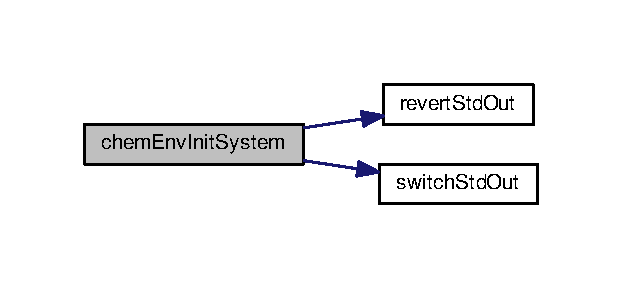
\includegraphics[width=298pt]{chemf_8c_abc9d0a6b17feeff2a62eb6bb38c17ff4_cgraph}
\end{center}
\end{figure}




Here is the caller graph for this function\-:\nopagebreak
\begin{figure}[H]
\begin{center}
\leavevmode
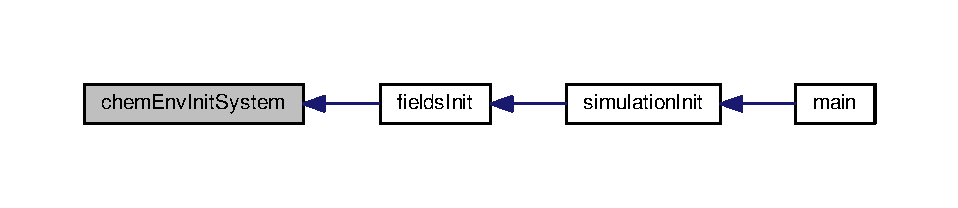
\includegraphics[width=350pt]{chemf_8c_abc9d0a6b17feeff2a62eb6bb38c17ff4_icgraph}
\end{center}
\end{figure}


\hypertarget{chemf_8c_a1f8f7d186d46aafcd792aaf3bee655a7}{\index{chemf.\-c@{chemf.\-c}!chem\-Env\-Solve@{chem\-Env\-Solve}}
\index{chem\-Env\-Solve@{chem\-Env\-Solve}!chemf.c@{chemf.\-c}}
\subsubsection[{chem\-Env\-Solve}]{\setlength{\rightskip}{0pt plus 5cm}void chem\-Env\-Solve (
\begin{DoxyParamCaption}
\item[{int}]{nch}
\end{DoxyParamCaption}
)}}\label{chemf_8c_a1f8f7d186d46aafcd792aaf3bee655a7}
This is a driving function for solving next time step of a given chemical field. 

Definition at line 431 of file chemf.\-c.



References bc\-Lower, bc\-Upper, chemb, chem\-Env\-Cell\-P\-C(), chem\-Field, chem\-Iter, chem\-Lower, chem\-Par\-A, chem\-Parb, chem\-Parx, chem\-P\-C, chem\-Set\-Boundary(), chem\-Solver, chem\-Upper, chemx, chem\-Z, chfname, field\-B\-C, field\-Max, field\-Min, field\-Name, gf\-Iter, gf\-Iter\-Per\-Step, grid\-Size, M\-P\-Icoords, M\-P\-Idim, M\-P\-Irank, N\-G\-L\-O\-B, number\-Of\-Iters, revert\-Std\-Out(), stat\-Out\-Step, step, switch\-Std\-Out(), int64\-Vector3d\-::x, int64\-Vector3d\-::y, and int64\-Vector3d\-::z.


\begin{DoxyCode}
432 \{
433   \textcolor{keywordtype}{int} i, j, k;
434   \textcolor{keywordtype}{int} idx;
435   \textcolor{keywordtype}{double} *values;
436   \textcolor{keywordtype}{int} stepIter = 0;
437   \textcolor{keywordtype}{long} \textcolor{keywordtype}{long} nvalues = \hyperlink{fields_8h_ae67bb9d09bd0919a0ccbc27b387cec72}{gridSize}.\hyperlink{structint64Vector3d_a040359f45343ce6667f5c66fda5f50e3}{x} * \hyperlink{fields_8h_ae67bb9d09bd0919a0ccbc27b387cec72}{gridSize}.\hyperlink{structint64Vector3d_a0cbcba26311a97b8e0763317e105a918}{y} * \hyperlink{fields_8h_ae67bb9d09bd0919a0ccbc27b387cec72}{gridSize}.
      \hyperlink{structint64Vector3d_a44624880ae3bb63041297b70cb33408b}{z};
438 \textcolor{preprocessor}{#ifdef DEBUG}
439 \textcolor{preprocessor}{}  \textcolor{keywordflow}{if} (\hyperlink{global_8h_a710288ab7d2734acc4566a87a645325d}{MPIrank} == 0 && !(\hyperlink{global_8h_abc16e65f240ed0c8f3e876e8732c0a33}{step} % \hyperlink{global_8h_aab9700fe12cc303ff43e1a35a210128e}{statOutStep}) && \hyperlink{global_8h_ab2e483b60cc15741bd6281688f31edbc}{gfIter} == 0) \{
440     printf(\textcolor{stringliteral}{" Solving field: %s..."}, \hyperlink{fields_8h_a1a12b04329495ce82cf21a9d42b71f1c}{fieldName}[nch + \hyperlink{fields_8h_aa40ca56600c708a797a77c1db484958d}{NGLOB}]);
441     fflush(stdout);
442   \}
443 \textcolor{preprocessor}{#endif}
444 \textcolor{preprocessor}{}  \textcolor{comment}{/* redirecting stdout to log file */}
445   \hyperlink{io_8c_a62f5074e9f833de4cbf65a82dbb2f81b}{switchStdOut}(\hyperlink{chemf_8c_a27dc1f70b41e3739d1629663a1d3d0a6}{chfname});
446 
447   values = (\textcolor{keywordtype}{double} *) calloc(nvalues, \textcolor{keyword}{sizeof}(\textcolor{keywordtype}{double}));
448   \hyperlink{chemf_8c_a614434a804d9a302d1db9603c22b60a7}{chemPC} = (\textcolor{keywordtype}{double} *) calloc(nvalues, \textcolor{keyword}{sizeof}(\textcolor{keywordtype}{double}));
449   \hyperlink{chemf_8c_a5ca738b55b36899ceaa4fe1e6ff38b9f}{chemEnvCellPC}(nch);
450 
451   \hyperlink{fields_8h_adc4b9b908fa47243451f8725e6210e34}{fieldMin}[nch + \hyperlink{fields_8h_aa40ca56600c708a797a77c1db484958d}{NGLOB}] = DBL\_MAX;
452   \hyperlink{fields_8h_afa26584ead914a9e160c467308ed156a}{fieldMax}[nch + \hyperlink{fields_8h_aa40ca56600c708a797a77c1db484958d}{NGLOB}] = DBL\_MIN;
453 
454   \textcolor{keywordflow}{while} (stepIter < \hyperlink{chemf_8c_a07fef4b421caa5300b13b2ba89422841}{numberOfIters}) \{
455     \textcolor{keywordflow}{if} (\hyperlink{chemf_8c_a26adfe146e722023d7f81bf278bde9e7}{chemIter}[nch] > 0) \{
456       \textcolor{comment}{/* update right hand side */}
457       HYPRE\_SStructVectorGetBoxValues(\hyperlink{chemf_8c_a48c5bcbe8787c6a6be2a6d5bcdae101f}{chemx}[nch], 0, \hyperlink{chemf_8c_a14199fec6ea96fe4a4c57bccaff2dfe7}{chemLower}, 
      \hyperlink{chemf_8c_a019f631b2e2795023bf22abef7d9f80e}{chemUpper},
458                       0, values);
459       HYPRE\_SStructVectorSetBoxValues(\hyperlink{chemf_8c_afb43e9c9d8160250a03e1b41902473fd}{chemb}[nch], 0, \hyperlink{chemf_8c_a14199fec6ea96fe4a4c57bccaff2dfe7}{chemLower}, 
      \hyperlink{chemf_8c_a019f631b2e2795023bf22abef7d9f80e}{chemUpper},
460                       0, values);
461       \textcolor{keywordflow}{for} (i = 0; i < nvalues; i++)
462     values[i] = \hyperlink{chemf_8c_ad1178dce1f62833a078c63e911e2e023}{chemZ}[nch] * \hyperlink{fields_8h_a80c6ee80e0f056adba2430ab0d21e58f}{fieldBC}[nch + \hyperlink{fields_8h_aa40ca56600c708a797a77c1db484958d}{NGLOB}];
463       \textcolor{keywordflow}{if} (\hyperlink{global_8h_a8220294108e39b58632993a50a7dc4ca}{MPIcoords}[\hyperlink{global_8h_a710288ab7d2734acc4566a87a645325d}{MPIrank}][0] == 0) \{
464     \hyperlink{chemf_8c_afb692f34ea05262db93f9bf9590b06a7}{chemSetBoundary}(0, -1);
465     HYPRE\_SStructVectorAddToBoxValues(\hyperlink{chemf_8c_afb43e9c9d8160250a03e1b41902473fd}{chemb}[nch], 0, \hyperlink{chemf_8c_a397798166a570960b5d468b6df8bf02c}{bcLower}, 
      \hyperlink{chemf_8c_aaea99b8c85fcedb15091dcac991999fd}{bcUpper},
466                       0, values);
467       \}
468       \textcolor{keywordflow}{if} (\hyperlink{global_8h_a8220294108e39b58632993a50a7dc4ca}{MPIcoords}[\hyperlink{global_8h_a710288ab7d2734acc4566a87a645325d}{MPIrank}][0] == \hyperlink{global_8h_a633835398408aaee46fd56809af73e6c}{MPIdim}[0] - 1) \{
469     \hyperlink{chemf_8c_afb692f34ea05262db93f9bf9590b06a7}{chemSetBoundary}(0, 1);
470     HYPRE\_SStructVectorAddToBoxValues(\hyperlink{chemf_8c_afb43e9c9d8160250a03e1b41902473fd}{chemb}[nch], 0, \hyperlink{chemf_8c_a397798166a570960b5d468b6df8bf02c}{bcLower}, 
      \hyperlink{chemf_8c_aaea99b8c85fcedb15091dcac991999fd}{bcUpper},
471                       0, values);
472       \}
473       \textcolor{keywordflow}{if} (\hyperlink{global_8h_a8220294108e39b58632993a50a7dc4ca}{MPIcoords}[\hyperlink{global_8h_a710288ab7d2734acc4566a87a645325d}{MPIrank}][1] == 0) \{
474     \hyperlink{chemf_8c_afb692f34ea05262db93f9bf9590b06a7}{chemSetBoundary}(1, -1);
475     HYPRE\_SStructVectorAddToBoxValues(\hyperlink{chemf_8c_afb43e9c9d8160250a03e1b41902473fd}{chemb}[nch], 0, \hyperlink{chemf_8c_a397798166a570960b5d468b6df8bf02c}{bcLower}, 
      \hyperlink{chemf_8c_aaea99b8c85fcedb15091dcac991999fd}{bcUpper},
476                       0, values);
477       \}
478       \textcolor{keywordflow}{if} (\hyperlink{global_8h_a8220294108e39b58632993a50a7dc4ca}{MPIcoords}[\hyperlink{global_8h_a710288ab7d2734acc4566a87a645325d}{MPIrank}][1] == \hyperlink{global_8h_a633835398408aaee46fd56809af73e6c}{MPIdim}[1] - 1) \{
479     \hyperlink{chemf_8c_afb692f34ea05262db93f9bf9590b06a7}{chemSetBoundary}(1, 1);
480     HYPRE\_SStructVectorAddToBoxValues(\hyperlink{chemf_8c_afb43e9c9d8160250a03e1b41902473fd}{chemb}[nch], 0, \hyperlink{chemf_8c_a397798166a570960b5d468b6df8bf02c}{bcLower}, 
      \hyperlink{chemf_8c_aaea99b8c85fcedb15091dcac991999fd}{bcUpper},
481                       0, values);
482       \}
483       \textcolor{keywordflow}{if} (\hyperlink{global_8h_a8220294108e39b58632993a50a7dc4ca}{MPIcoords}[\hyperlink{global_8h_a710288ab7d2734acc4566a87a645325d}{MPIrank}][2] == 0) \{
484     \hyperlink{chemf_8c_afb692f34ea05262db93f9bf9590b06a7}{chemSetBoundary}(2, -1);
485     HYPRE\_SStructVectorAddToBoxValues(\hyperlink{chemf_8c_afb43e9c9d8160250a03e1b41902473fd}{chemb}[nch], 0, \hyperlink{chemf_8c_a397798166a570960b5d468b6df8bf02c}{bcLower}, 
      \hyperlink{chemf_8c_aaea99b8c85fcedb15091dcac991999fd}{bcUpper},
486                       0, values);
487       \}
488       \textcolor{keywordflow}{if} (\hyperlink{global_8h_a8220294108e39b58632993a50a7dc4ca}{MPIcoords}[\hyperlink{global_8h_a710288ab7d2734acc4566a87a645325d}{MPIrank}][2] == \hyperlink{global_8h_a633835398408aaee46fd56809af73e6c}{MPIdim}[2] - 1) \{
489     \hyperlink{chemf_8c_afb692f34ea05262db93f9bf9590b06a7}{chemSetBoundary}(2, 1);
490     HYPRE\_SStructVectorAddToBoxValues(\hyperlink{chemf_8c_afb43e9c9d8160250a03e1b41902473fd}{chemb}[nch], 0, \hyperlink{chemf_8c_a397798166a570960b5d468b6df8bf02c}{bcLower}, 
      \hyperlink{chemf_8c_aaea99b8c85fcedb15091dcac991999fd}{bcUpper},
491                       0, values);
492       \}
493       HYPRE\_SStructVectorAddToBoxValues(\hyperlink{chemf_8c_afb43e9c9d8160250a03e1b41902473fd}{chemb}[nch], 0, \hyperlink{chemf_8c_a14199fec6ea96fe4a4c57bccaff2dfe7}{chemLower},
494                     \hyperlink{chemf_8c_a019f631b2e2795023bf22abef7d9f80e}{chemUpper}, 0, \hyperlink{chemf_8c_a614434a804d9a302d1db9603c22b60a7}{chemPC});
495       HYPRE\_SStructVectorAssemble(\hyperlink{chemf_8c_afb43e9c9d8160250a03e1b41902473fd}{chemb}[nch]);
496       HYPRE\_SStructVectorAssemble(\hyperlink{chemf_8c_a48c5bcbe8787c6a6be2a6d5bcdae101f}{chemx}[nch]);
497     \}
498 
499     HYPRE\_ParCSRPCGSolve(\hyperlink{chemf_8c_a99bbb7b0352d9c850e98287fa45b42c0}{chemSolver}[nch], \hyperlink{chemf_8c_a998a7ebb65eb001abcee46c1ea1b1756}{chemParA}[nch], 
      \hyperlink{chemf_8c_af74b7f36ec77fb8e0638db98dd2ee47a}{chemParb}[nch],
500              \hyperlink{chemf_8c_aae118f98b57f3dda9f036d39db247bb1}{chemParx}[nch]);
501 
502     \textcolor{comment}{/* copy solution to field buffer */}
503     HYPRE\_SStructVectorGather(\hyperlink{chemf_8c_a48c5bcbe8787c6a6be2a6d5bcdae101f}{chemx}[nch]);
504     HYPRE\_SStructVectorGetBoxValues(\hyperlink{chemf_8c_a48c5bcbe8787c6a6be2a6d5bcdae101f}{chemx}[nch], 0, \hyperlink{chemf_8c_a14199fec6ea96fe4a4c57bccaff2dfe7}{chemLower}, 
      \hyperlink{chemf_8c_a019f631b2e2795023bf22abef7d9f80e}{chemUpper}, 0,
505                     values);
506     idx = 0;
507     \textcolor{keywordflow}{for} (k = 0; k < \hyperlink{fields_8h_ae67bb9d09bd0919a0ccbc27b387cec72}{gridSize}.\hyperlink{structint64Vector3d_a44624880ae3bb63041297b70cb33408b}{z}; k++)
508       \textcolor{keywordflow}{for} (j = 0; j < \hyperlink{fields_8h_ae67bb9d09bd0919a0ccbc27b387cec72}{gridSize}.\hyperlink{structint64Vector3d_a0cbcba26311a97b8e0763317e105a918}{y}; j++)
509     \textcolor{keywordflow}{for} (i = 0; i < \hyperlink{fields_8h_ae67bb9d09bd0919a0ccbc27b387cec72}{gridSize}.\hyperlink{structint64Vector3d_a040359f45343ce6667f5c66fda5f50e3}{x}; i++, idx++) \{
510       \hyperlink{fields_8h_adb9b18c97bd0384bf977ee57e604626a}{chemField}[nch][\hyperlink{fields_8h_ae67bb9d09bd0919a0ccbc27b387cec72}{gridSize}.\hyperlink{structint64Vector3d_a0cbcba26311a97b8e0763317e105a918}{y} * \hyperlink{fields_8h_ae67bb9d09bd0919a0ccbc27b387cec72}{gridSize}.\hyperlink{structint64Vector3d_a44624880ae3bb63041297b70cb33408b}{z} * i + 
      \hyperlink{fields_8h_ae67bb9d09bd0919a0ccbc27b387cec72}{gridSize}.\hyperlink{structint64Vector3d_a44624880ae3bb63041297b70cb33408b}{z} * j +
511              k] = values[idx];
512       \textcolor{keywordflow}{if} (values[idx] > \hyperlink{fields_8h_afa26584ead914a9e160c467308ed156a}{fieldMax}[nch + \hyperlink{fields_8h_aa40ca56600c708a797a77c1db484958d}{NGLOB}])
513         \hyperlink{fields_8h_afa26584ead914a9e160c467308ed156a}{fieldMax}[nch + \hyperlink{fields_8h_aa40ca56600c708a797a77c1db484958d}{NGLOB}] = values[idx];
514       \textcolor{keywordflow}{if} (values[idx] < \hyperlink{fields_8h_adc4b9b908fa47243451f8725e6210e34}{fieldMin}[nch + \hyperlink{fields_8h_aa40ca56600c708a797a77c1db484958d}{NGLOB}])
515         \hyperlink{fields_8h_adc4b9b908fa47243451f8725e6210e34}{fieldMin}[nch + \hyperlink{fields_8h_aa40ca56600c708a797a77c1db484958d}{NGLOB}] = values[idx];
516     \}
517     \hyperlink{chemf_8c_a26adfe146e722023d7f81bf278bde9e7}{chemIter}[nch]++;
518     stepIter++;
519   \}
520 
521   free(values);
522   free(\hyperlink{chemf_8c_a614434a804d9a302d1db9603c22b60a7}{chemPC});
523   \textcolor{comment}{/* stdout brought back */}
524   \hyperlink{io_8c_affa00173da9bea48973a6ac887d505bb}{revertStdOut}();
525 \textcolor{preprocessor}{#ifdef DEBUG}
526 \textcolor{preprocessor}{}  \textcolor{keywordflow}{if} (\hyperlink{global_8h_a710288ab7d2734acc4566a87a645325d}{MPIrank} == 0 && !(\hyperlink{global_8h_abc16e65f240ed0c8f3e876e8732c0a33}{step} % statOutStep) && \hyperlink{global_8h_ab2e483b60cc15741bd6281688f31edbc}{gfIter} == 
      \hyperlink{global_8h_a4b76c15679db05e32f70c9804e186557}{gfIterPerStep} - 1) \{
527     printf(\textcolor{stringliteral}{"done\(\backslash\)n"});
528     fflush(stdout);
529   \}
530 \textcolor{preprocessor}{#endif}
531 \textcolor{preprocessor}{}\}
\end{DoxyCode}


Here is the call graph for this function\-:\nopagebreak
\begin{figure}[H]
\begin{center}
\leavevmode
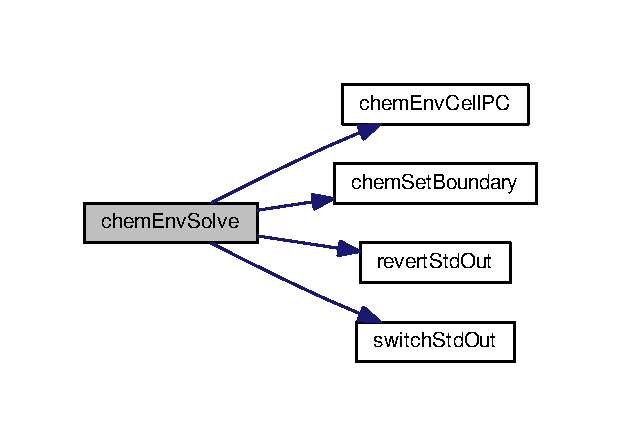
\includegraphics[width=298pt]{chemf_8c_a1f8f7d186d46aafcd792aaf3bee655a7_cgraph}
\end{center}
\end{figure}




Here is the caller graph for this function\-:\nopagebreak
\begin{figure}[H]
\begin{center}
\leavevmode
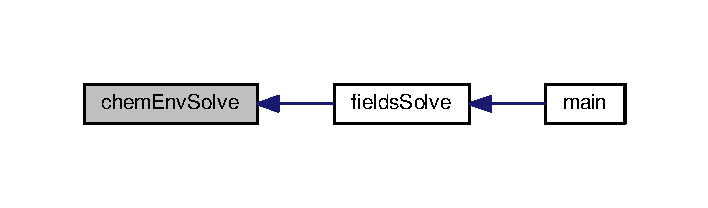
\includegraphics[width=340pt]{chemf_8c_a1f8f7d186d46aafcd792aaf3bee655a7_icgraph}
\end{center}
\end{figure}


\hypertarget{chemf_8c_afb692f34ea05262db93f9bf9590b06a7}{\index{chemf.\-c@{chemf.\-c}!chem\-Set\-Boundary@{chem\-Set\-Boundary}}
\index{chem\-Set\-Boundary@{chem\-Set\-Boundary}!chemf.c@{chemf.\-c}}
\subsubsection[{chem\-Set\-Boundary}]{\setlength{\rightskip}{0pt plus 5cm}void chem\-Set\-Boundary (
\begin{DoxyParamCaption}
\item[{int}]{coord, }
\item[{int}]{boundary}
\end{DoxyParamCaption}
)}}\label{chemf_8c_afb692f34ea05262db93f9bf9590b06a7}
This function sets boundary conditions for domain faces. 

Definition at line 75 of file chemf.\-c.



References bc\-Lower, bc\-Upper, chem\-Lower, and chem\-Upper.


\begin{DoxyCode}
76 \{
77   \textcolor{keywordflow}{if} (coord == 0 && boundary == -1) \{
78     \hyperlink{chemf_8c_a397798166a570960b5d468b6df8bf02c}{bcLower}[0] = \hyperlink{chemf_8c_a14199fec6ea96fe4a4c57bccaff2dfe7}{chemLower}[0];
79     \hyperlink{chemf_8c_aaea99b8c85fcedb15091dcac991999fd}{bcUpper}[0] = \hyperlink{chemf_8c_a14199fec6ea96fe4a4c57bccaff2dfe7}{chemLower}[0];
80     \hyperlink{chemf_8c_a397798166a570960b5d468b6df8bf02c}{bcLower}[1] = \hyperlink{chemf_8c_a14199fec6ea96fe4a4c57bccaff2dfe7}{chemLower}[1];
81     \hyperlink{chemf_8c_aaea99b8c85fcedb15091dcac991999fd}{bcUpper}[1] = \hyperlink{chemf_8c_a019f631b2e2795023bf22abef7d9f80e}{chemUpper}[1];
82     \hyperlink{chemf_8c_a397798166a570960b5d468b6df8bf02c}{bcLower}[2] = \hyperlink{chemf_8c_a14199fec6ea96fe4a4c57bccaff2dfe7}{chemLower}[2];
83     \hyperlink{chemf_8c_aaea99b8c85fcedb15091dcac991999fd}{bcUpper}[2] = \hyperlink{chemf_8c_a019f631b2e2795023bf22abef7d9f80e}{chemUpper}[2];
84   \}
85   \textcolor{keywordflow}{if} (coord == 0 && boundary == 1) \{
86     \hyperlink{chemf_8c_a397798166a570960b5d468b6df8bf02c}{bcLower}[0] = \hyperlink{chemf_8c_a019f631b2e2795023bf22abef7d9f80e}{chemUpper}[0];
87     \hyperlink{chemf_8c_aaea99b8c85fcedb15091dcac991999fd}{bcUpper}[0] = \hyperlink{chemf_8c_a019f631b2e2795023bf22abef7d9f80e}{chemUpper}[0];
88     \hyperlink{chemf_8c_a397798166a570960b5d468b6df8bf02c}{bcLower}[1] = \hyperlink{chemf_8c_a14199fec6ea96fe4a4c57bccaff2dfe7}{chemLower}[1];
89     \hyperlink{chemf_8c_aaea99b8c85fcedb15091dcac991999fd}{bcUpper}[1] = \hyperlink{chemf_8c_a019f631b2e2795023bf22abef7d9f80e}{chemUpper}[1];
90     \hyperlink{chemf_8c_a397798166a570960b5d468b6df8bf02c}{bcLower}[2] = \hyperlink{chemf_8c_a14199fec6ea96fe4a4c57bccaff2dfe7}{chemLower}[2];
91     \hyperlink{chemf_8c_aaea99b8c85fcedb15091dcac991999fd}{bcUpper}[2] = \hyperlink{chemf_8c_a019f631b2e2795023bf22abef7d9f80e}{chemUpper}[2];
92   \}
93   \textcolor{keywordflow}{if} (coord == 1 && boundary == -1) \{
94     \hyperlink{chemf_8c_a397798166a570960b5d468b6df8bf02c}{bcLower}[0] = \hyperlink{chemf_8c_a14199fec6ea96fe4a4c57bccaff2dfe7}{chemLower}[0];
95     \hyperlink{chemf_8c_aaea99b8c85fcedb15091dcac991999fd}{bcUpper}[0] = \hyperlink{chemf_8c_a019f631b2e2795023bf22abef7d9f80e}{chemUpper}[0];
96     \hyperlink{chemf_8c_a397798166a570960b5d468b6df8bf02c}{bcLower}[1] = \hyperlink{chemf_8c_a14199fec6ea96fe4a4c57bccaff2dfe7}{chemLower}[1];
97     \hyperlink{chemf_8c_aaea99b8c85fcedb15091dcac991999fd}{bcUpper}[1] = \hyperlink{chemf_8c_a14199fec6ea96fe4a4c57bccaff2dfe7}{chemLower}[1];
98     \hyperlink{chemf_8c_a397798166a570960b5d468b6df8bf02c}{bcLower}[2] = \hyperlink{chemf_8c_a14199fec6ea96fe4a4c57bccaff2dfe7}{chemLower}[2];
99     \hyperlink{chemf_8c_aaea99b8c85fcedb15091dcac991999fd}{bcUpper}[2] = \hyperlink{chemf_8c_a019f631b2e2795023bf22abef7d9f80e}{chemUpper}[2];
100   \}
101   \textcolor{keywordflow}{if} (coord == 1 && boundary == 1) \{
102     \hyperlink{chemf_8c_a397798166a570960b5d468b6df8bf02c}{bcLower}[0] = \hyperlink{chemf_8c_a14199fec6ea96fe4a4c57bccaff2dfe7}{chemLower}[0];
103     \hyperlink{chemf_8c_aaea99b8c85fcedb15091dcac991999fd}{bcUpper}[0] = \hyperlink{chemf_8c_a019f631b2e2795023bf22abef7d9f80e}{chemUpper}[0];
104     \hyperlink{chemf_8c_a397798166a570960b5d468b6df8bf02c}{bcLower}[1] = \hyperlink{chemf_8c_a019f631b2e2795023bf22abef7d9f80e}{chemUpper}[1];
105     \hyperlink{chemf_8c_aaea99b8c85fcedb15091dcac991999fd}{bcUpper}[1] = \hyperlink{chemf_8c_a019f631b2e2795023bf22abef7d9f80e}{chemUpper}[1];
106     \hyperlink{chemf_8c_a397798166a570960b5d468b6df8bf02c}{bcLower}[2] = \hyperlink{chemf_8c_a14199fec6ea96fe4a4c57bccaff2dfe7}{chemLower}[2];
107     \hyperlink{chemf_8c_aaea99b8c85fcedb15091dcac991999fd}{bcUpper}[2] = \hyperlink{chemf_8c_a019f631b2e2795023bf22abef7d9f80e}{chemUpper}[2];
108   \}
109   \textcolor{keywordflow}{if} (coord == 2 && boundary == -1) \{
110     \hyperlink{chemf_8c_a397798166a570960b5d468b6df8bf02c}{bcLower}[0] = \hyperlink{chemf_8c_a14199fec6ea96fe4a4c57bccaff2dfe7}{chemLower}[0];
111     \hyperlink{chemf_8c_aaea99b8c85fcedb15091dcac991999fd}{bcUpper}[0] = \hyperlink{chemf_8c_a019f631b2e2795023bf22abef7d9f80e}{chemUpper}[0];
112     \hyperlink{chemf_8c_a397798166a570960b5d468b6df8bf02c}{bcLower}[1] = \hyperlink{chemf_8c_a14199fec6ea96fe4a4c57bccaff2dfe7}{chemLower}[1];
113     \hyperlink{chemf_8c_aaea99b8c85fcedb15091dcac991999fd}{bcUpper}[1] = \hyperlink{chemf_8c_a019f631b2e2795023bf22abef7d9f80e}{chemUpper}[1];
114     \hyperlink{chemf_8c_a397798166a570960b5d468b6df8bf02c}{bcLower}[2] = \hyperlink{chemf_8c_a14199fec6ea96fe4a4c57bccaff2dfe7}{chemLower}[2];
115     \hyperlink{chemf_8c_aaea99b8c85fcedb15091dcac991999fd}{bcUpper}[2] = \hyperlink{chemf_8c_a14199fec6ea96fe4a4c57bccaff2dfe7}{chemLower}[2];
116   \}
117   \textcolor{keywordflow}{if} (coord == 2 && boundary == 1) \{
118     \hyperlink{chemf_8c_a397798166a570960b5d468b6df8bf02c}{bcLower}[0] = \hyperlink{chemf_8c_a14199fec6ea96fe4a4c57bccaff2dfe7}{chemLower}[0];
119     \hyperlink{chemf_8c_aaea99b8c85fcedb15091dcac991999fd}{bcUpper}[0] = \hyperlink{chemf_8c_a019f631b2e2795023bf22abef7d9f80e}{chemUpper}[0];
120     \hyperlink{chemf_8c_a397798166a570960b5d468b6df8bf02c}{bcLower}[1] = \hyperlink{chemf_8c_a14199fec6ea96fe4a4c57bccaff2dfe7}{chemLower}[1];
121     \hyperlink{chemf_8c_aaea99b8c85fcedb15091dcac991999fd}{bcUpper}[1] = \hyperlink{chemf_8c_a019f631b2e2795023bf22abef7d9f80e}{chemUpper}[1];
122     \hyperlink{chemf_8c_a397798166a570960b5d468b6df8bf02c}{bcLower}[2] = \hyperlink{chemf_8c_a019f631b2e2795023bf22abef7d9f80e}{chemUpper}[2];
123     \hyperlink{chemf_8c_aaea99b8c85fcedb15091dcac991999fd}{bcUpper}[2] = \hyperlink{chemf_8c_a019f631b2e2795023bf22abef7d9f80e}{chemUpper}[2];
124   \}
125 \}
\end{DoxyCode}


Here is the caller graph for this function\-:\nopagebreak
\begin{figure}[H]
\begin{center}
\leavevmode
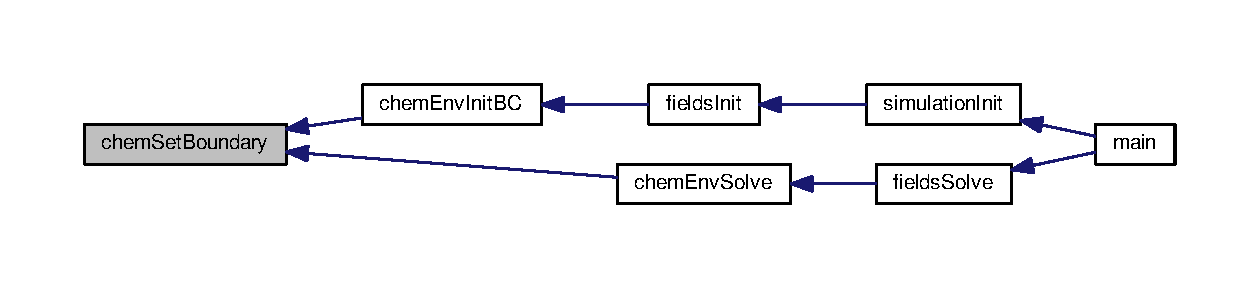
\includegraphics[width=350pt]{chemf_8c_afb692f34ea05262db93f9bf9590b06a7_icgraph}
\end{center}
\end{figure}




\subsection{Variable Documentation}
\hypertarget{chemf_8c_a397798166a570960b5d468b6df8bf02c}{\index{chemf.\-c@{chemf.\-c}!bc\-Lower@{bc\-Lower}}
\index{bc\-Lower@{bc\-Lower}!chemf.c@{chemf.\-c}}
\subsubsection[{bc\-Lower}]{\setlength{\rightskip}{0pt plus 5cm}long long bc\-Lower\mbox{[}3\mbox{]}}}\label{chemf_8c_a397798166a570960b5d468b6df8bf02c}


Definition at line 54 of file chemf.\-c.

\hypertarget{chemf_8c_aaea99b8c85fcedb15091dcac991999fd}{\index{chemf.\-c@{chemf.\-c}!bc\-Upper@{bc\-Upper}}
\index{bc\-Upper@{bc\-Upper}!chemf.c@{chemf.\-c}}
\subsubsection[{bc\-Upper}]{\setlength{\rightskip}{0pt plus 5cm}long long bc\-Upper\mbox{[}3\mbox{]}}}\label{chemf_8c_aaea99b8c85fcedb15091dcac991999fd}


Definition at line 55 of file chemf.\-c.

\hypertarget{chemf_8c_ad634e858729e0c04e8b9a4b0a1144b10}{\index{chemf.\-c@{chemf.\-c}!chem\-A@{chem\-A}}
\index{chem\-A@{chem\-A}!chemf.c@{chemf.\-c}}
\subsubsection[{chem\-A}]{\setlength{\rightskip}{0pt plus 5cm}H\-Y\-P\-R\-E\-\_\-\-S\-Struct\-Matrix chem\-A\mbox{[}{\bf N\-C\-H\-E\-M}\mbox{]}}}\label{chemf_8c_ad634e858729e0c04e8b9a4b0a1144b10}


Definition at line 40 of file chemf.\-c.

\hypertarget{chemf_8c_afb43e9c9d8160250a03e1b41902473fd}{\index{chemf.\-c@{chemf.\-c}!chemb@{chemb}}
\index{chemb@{chemb}!chemf.c@{chemf.\-c}}
\subsubsection[{chemb}]{\setlength{\rightskip}{0pt plus 5cm}H\-Y\-P\-R\-E\-\_\-\-S\-Struct\-Vector chemb\mbox{[}{\bf N\-C\-H\-E\-M}\mbox{]}}}\label{chemf_8c_afb43e9c9d8160250a03e1b41902473fd}


Definition at line 41 of file chemf.\-c.

\hypertarget{chemf_8c_aaac58de32c5dda56ce31654ec3e19337}{\index{chemf.\-c@{chemf.\-c}!chem\-Graph@{chem\-Graph}}
\index{chem\-Graph@{chem\-Graph}!chemf.c@{chemf.\-c}}
\subsubsection[{chem\-Graph}]{\setlength{\rightskip}{0pt plus 5cm}H\-Y\-P\-R\-E\-\_\-\-S\-Struct\-Graph chem\-Graph\mbox{[}{\bf N\-C\-H\-E\-M}\mbox{]}}}\label{chemf_8c_aaac58de32c5dda56ce31654ec3e19337}


Definition at line 37 of file chemf.\-c.

\hypertarget{chemf_8c_ad7a28a5fc279e8b757bdc6a4b57c25be}{\index{chemf.\-c@{chemf.\-c}!chem\-Grid@{chem\-Grid}}
\index{chem\-Grid@{chem\-Grid}!chemf.c@{chemf.\-c}}
\subsubsection[{chem\-Grid}]{\setlength{\rightskip}{0pt plus 5cm}H\-Y\-P\-R\-E\-\_\-\-S\-Struct\-Grid chem\-Grid\mbox{[}{\bf N\-C\-H\-E\-M}\mbox{]}}}\label{chemf_8c_ad7a28a5fc279e8b757bdc6a4b57c25be}


Definition at line 36 of file chemf.\-c.

\hypertarget{chemf_8c_a26adfe146e722023d7f81bf278bde9e7}{\index{chemf.\-c@{chemf.\-c}!chem\-Iter@{chem\-Iter}}
\index{chem\-Iter@{chem\-Iter}!chemf.c@{chemf.\-c}}
\subsubsection[{chem\-Iter}]{\setlength{\rightskip}{0pt plus 5cm}int chem\-Iter\mbox{[}{\bf N\-C\-H\-E\-M}\mbox{]}}}\label{chemf_8c_a26adfe146e722023d7f81bf278bde9e7}


Definition at line 62 of file chemf.\-c.

\hypertarget{chemf_8c_ab35147d777155659aaad43553e3378f4}{\index{chemf.\-c@{chemf.\-c}!chem\-Lambda@{chem\-Lambda}}
\index{chem\-Lambda@{chem\-Lambda}!chemf.c@{chemf.\-c}}
\subsubsection[{chem\-Lambda}]{\setlength{\rightskip}{0pt plus 5cm}double chem\-Lambda = 0.\-25}}\label{chemf_8c_ab35147d777155659aaad43553e3378f4}


Definition at line 58 of file chemf.\-c.

\hypertarget{chemf_8c_a14199fec6ea96fe4a4c57bccaff2dfe7}{\index{chemf.\-c@{chemf.\-c}!chem\-Lower@{chem\-Lower}}
\index{chem\-Lower@{chem\-Lower}!chemf.c@{chemf.\-c}}
\subsubsection[{chem\-Lower}]{\setlength{\rightskip}{0pt plus 5cm}long long chem\-Lower\mbox{[}3\mbox{]}}}\label{chemf_8c_a14199fec6ea96fe4a4c57bccaff2dfe7}


Definition at line 53 of file chemf.\-c.

\hypertarget{chemf_8c_a242fb3ba38fb1c6054fd05507394f08b}{\index{chemf.\-c@{chemf.\-c}!chem\-Object\-Type@{chem\-Object\-Type}}
\index{chem\-Object\-Type@{chem\-Object\-Type}!chemf.c@{chemf.\-c}}
\subsubsection[{chem\-Object\-Type}]{\setlength{\rightskip}{0pt plus 5cm}int chem\-Object\-Type}}\label{chemf_8c_a242fb3ba38fb1c6054fd05507394f08b}


Definition at line 51 of file chemf.\-c.

\hypertarget{chemf_8c_a998a7ebb65eb001abcee46c1ea1b1756}{\index{chemf.\-c@{chemf.\-c}!chem\-Par\-A@{chem\-Par\-A}}
\index{chem\-Par\-A@{chem\-Par\-A}!chemf.c@{chemf.\-c}}
\subsubsection[{chem\-Par\-A}]{\setlength{\rightskip}{0pt plus 5cm}H\-Y\-P\-R\-E\-\_\-\-Par\-C\-S\-R\-Matrix chem\-Par\-A\mbox{[}{\bf N\-C\-H\-E\-M}\mbox{]}}}\label{chemf_8c_a998a7ebb65eb001abcee46c1ea1b1756}


Definition at line 44 of file chemf.\-c.

\hypertarget{chemf_8c_af74b7f36ec77fb8e0638db98dd2ee47a}{\index{chemf.\-c@{chemf.\-c}!chem\-Parb@{chem\-Parb}}
\index{chem\-Parb@{chem\-Parb}!chemf.c@{chemf.\-c}}
\subsubsection[{chem\-Parb}]{\setlength{\rightskip}{0pt plus 5cm}H\-Y\-P\-R\-E\-\_\-\-Par\-Vector chem\-Parb\mbox{[}{\bf N\-C\-H\-E\-M}\mbox{]}}}\label{chemf_8c_af74b7f36ec77fb8e0638db98dd2ee47a}


Definition at line 45 of file chemf.\-c.

\hypertarget{chemf_8c_aae118f98b57f3dda9f036d39db247bb1}{\index{chemf.\-c@{chemf.\-c}!chem\-Parx@{chem\-Parx}}
\index{chem\-Parx@{chem\-Parx}!chemf.c@{chemf.\-c}}
\subsubsection[{chem\-Parx}]{\setlength{\rightskip}{0pt plus 5cm}H\-Y\-P\-R\-E\-\_\-\-Par\-Vector chem\-Parx\mbox{[}{\bf N\-C\-H\-E\-M}\mbox{]}}}\label{chemf_8c_aae118f98b57f3dda9f036d39db247bb1}


Definition at line 46 of file chemf.\-c.

\hypertarget{chemf_8c_a614434a804d9a302d1db9603c22b60a7}{\index{chemf.\-c@{chemf.\-c}!chem\-P\-C@{chem\-P\-C}}
\index{chem\-P\-C@{chem\-P\-C}!chemf.c@{chemf.\-c}}
\subsubsection[{chem\-P\-C}]{\setlength{\rightskip}{0pt plus 5cm}double$\ast$ chem\-P\-C}}\label{chemf_8c_a614434a804d9a302d1db9603c22b60a7}


Definition at line 70 of file chemf.\-c.

\hypertarget{chemf_8c_a91747632f47bf551e8915e343439777f}{\index{chemf.\-c@{chemf.\-c}!chem\-Precond@{chem\-Precond}}
\index{chem\-Precond@{chem\-Precond}!chemf.c@{chemf.\-c}}
\subsubsection[{chem\-Precond}]{\setlength{\rightskip}{0pt plus 5cm}H\-Y\-P\-R\-E\-\_\-\-Solver chem\-Precond\mbox{[}{\bf N\-C\-H\-E\-M}\mbox{]}}}\label{chemf_8c_a91747632f47bf551e8915e343439777f}


Definition at line 49 of file chemf.\-c.

\hypertarget{chemf_8c_a99bbb7b0352d9c850e98287fa45b42c0}{\index{chemf.\-c@{chemf.\-c}!chem\-Solver@{chem\-Solver}}
\index{chem\-Solver@{chem\-Solver}!chemf.c@{chemf.\-c}}
\subsubsection[{chem\-Solver}]{\setlength{\rightskip}{0pt plus 5cm}H\-Y\-P\-R\-E\-\_\-\-Solver chem\-Solver\mbox{[}{\bf N\-C\-H\-E\-M}\mbox{]}}}\label{chemf_8c_a99bbb7b0352d9c850e98287fa45b42c0}


Definition at line 48 of file chemf.\-c.

\hypertarget{chemf_8c_ae8a36b5c7c6256a7d248a08c71944c73}{\index{chemf.\-c@{chemf.\-c}!chem\-Stencil@{chem\-Stencil}}
\index{chem\-Stencil@{chem\-Stencil}!chemf.c@{chemf.\-c}}
\subsubsection[{chem\-Stencil}]{\setlength{\rightskip}{0pt plus 5cm}H\-Y\-P\-R\-E\-\_\-\-S\-Struct\-Stencil chem\-Stencil\mbox{[}{\bf N\-C\-H\-E\-M}\mbox{]}}}\label{chemf_8c_ae8a36b5c7c6256a7d248a08c71944c73}


Definition at line 38 of file chemf.\-c.

\hypertarget{chemf_8c_a019f631b2e2795023bf22abef7d9f80e}{\index{chemf.\-c@{chemf.\-c}!chem\-Upper@{chem\-Upper}}
\index{chem\-Upper@{chem\-Upper}!chemf.c@{chemf.\-c}}
\subsubsection[{chem\-Upper}]{\setlength{\rightskip}{0pt plus 5cm}long long chem\-Upper\mbox{[}3\mbox{]}}}\label{chemf_8c_a019f631b2e2795023bf22abef7d9f80e}


Definition at line 53 of file chemf.\-c.

\hypertarget{chemf_8c_aa73fdbffdd3d43dd503718011b98e41f}{\index{chemf.\-c@{chemf.\-c}!chem\-Vartypes@{chem\-Vartypes}}
\index{chem\-Vartypes@{chem\-Vartypes}!chemf.c@{chemf.\-c}}
\subsubsection[{chem\-Vartypes}]{\setlength{\rightskip}{0pt plus 5cm}H\-Y\-P\-R\-E\-\_\-\-S\-Struct\-Variable chem\-Vartypes\mbox{[}1\mbox{]} = \{ H\-Y\-P\-R\-E\-\_\-\-S\-S\-T\-R\-U\-C\-T\-\_\-\-V\-A\-R\-I\-A\-B\-L\-E\-\_\-\-N\-O\-D\-E \}}}\label{chemf_8c_aa73fdbffdd3d43dd503718011b98e41f}


Definition at line 66 of file chemf.\-c.

\hypertarget{chemf_8c_a48c5bcbe8787c6a6be2a6d5bcdae101f}{\index{chemf.\-c@{chemf.\-c}!chemx@{chemx}}
\index{chemx@{chemx}!chemf.c@{chemf.\-c}}
\subsubsection[{chemx}]{\setlength{\rightskip}{0pt plus 5cm}H\-Y\-P\-R\-E\-\_\-\-S\-Struct\-Vector chemx\mbox{[}{\bf N\-C\-H\-E\-M}\mbox{]}}}\label{chemf_8c_a48c5bcbe8787c6a6be2a6d5bcdae101f}


Definition at line 42 of file chemf.\-c.

\hypertarget{chemf_8c_ad1178dce1f62833a078c63e911e2e023}{\index{chemf.\-c@{chemf.\-c}!chem\-Z@{chem\-Z}}
\index{chem\-Z@{chem\-Z}!chemf.c@{chemf.\-c}}
\subsubsection[{chem\-Z}]{\setlength{\rightskip}{0pt plus 5cm}double chem\-Z\mbox{[}{\bf N\-C\-H\-E\-M}\mbox{]}}}\label{chemf_8c_ad1178dce1f62833a078c63e911e2e023}


Definition at line 64 of file chemf.\-c.

\hypertarget{chemf_8c_a27dc1f70b41e3739d1629663a1d3d0a6}{\index{chemf.\-c@{chemf.\-c}!chfname@{chfname}}
\index{chfname@{chfname}!chemf.c@{chemf.\-c}}
\subsubsection[{chfname}]{\setlength{\rightskip}{0pt plus 5cm}char chfname\mbox{[}256\mbox{]}}}\label{chemf_8c_a27dc1f70b41e3739d1629663a1d3d0a6}


Definition at line 60 of file chemf.\-c.

\hypertarget{chemf_8c_a881c8c944ac83a5c022ee0e236f35e52}{\index{chemf.\-c@{chemf.\-c}!dt@{dt}}
\index{dt@{dt}!chemf.c@{chemf.\-c}}
\subsubsection[{dt}]{\setlength{\rightskip}{0pt plus 5cm}double dt\mbox{[}{\bf N\-C\-H\-E\-M}\mbox{]}}}\label{chemf_8c_a881c8c944ac83a5c022ee0e236f35e52}


Definition at line 57 of file chemf.\-c.

\hypertarget{chemf_8c_a07fef4b421caa5300b13b2ba89422841}{\index{chemf.\-c@{chemf.\-c}!number\-Of\-Iters@{number\-Of\-Iters}}
\index{number\-Of\-Iters@{number\-Of\-Iters}!chemf.c@{chemf.\-c}}
\subsubsection[{number\-Of\-Iters}]{\setlength{\rightskip}{0pt plus 5cm}int number\-Of\-Iters}}\label{chemf_8c_a07fef4b421caa5300b13b2ba89422841}


Definition at line 68 of file chemf.\-c.


\hypertarget{comm_8c}{\section{comm.\-c File Reference}
\label{comm_8c}\index{comm.\-c@{comm.\-c}}
}


contains communication functions  


{\ttfamily \#include $<$stdlib.\-h$>$}\\*
{\ttfamily \#include \char`\"{}global.\-h\char`\"{}}\\*
Include dependency graph for comm.\-c\-:\nopagebreak
\begin{figure}[H]
\begin{center}
\leavevmode
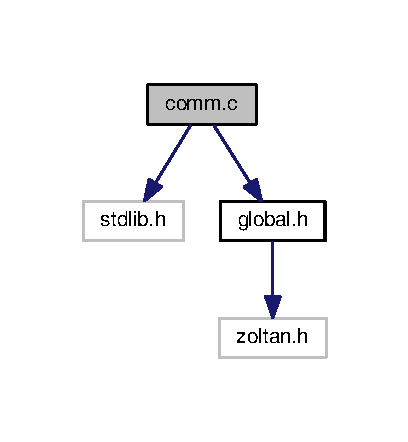
\includegraphics[width=196pt]{comm_8c__incl}
\end{center}
\end{figure}
\subsection*{Data Structures}
\begin{DoxyCompactItemize}
\item 
struct \hyperlink{structexpData}{exp\-Data}
\end{DoxyCompactItemize}
\subsection*{Macros}
\begin{DoxyCompactItemize}
\item 
\#define \hyperlink{comm_8c_a93da5acfae81b763e797f8562d49ca64}{M\-A\-X\-\_\-\-E\-X\-P\-O\-R\-T\-E\-D\-\_\-\-P\-E\-R\-\_\-\-P\-R\-O\-C}~2$\ast$\hyperlink{global_8h_a2de426dd266cfdaaf6fb52ba3dc2740a}{max\-Cells\-Per\-Proc}
\end{DoxyCompactItemize}
\subsection*{Functions}
\begin{DoxyCompactItemize}
\item 
int \hyperlink{comm_8c_a0a0b21ecf1a24a3cae73074d6bf6c68e}{comm\-\_\-compare\-\_\-exp\-\_\-list} (const void $\ast$a, const void $\ast$\hyperlink{tempf_8c_a74a523afdfebddf9b6b280e545977c5a}{b})
\item 
void \hyperlink{comm_8c_a191bffd6b8283bf118dec0d0422fa2b3}{create\-Export\-List} ()
\item 
void \hyperlink{comm_8c_abdd72f1d40c6c4bf47ad78c4f3c349d5}{comm\-Cleanup} ()
\item 
void \hyperlink{comm_8c_aa92fc6732720bc9accbbdef7fb02384f}{cells\-Exchange\-Init} ()
\item 
void \hyperlink{comm_8c_ac5b7dbd1157ef088c4e6f8a9f08fcc4b}{cells\-Exchange\-Wait} ()
\item 
void \hyperlink{comm_8c_a206e073b7e35f281184b3487b3bbc055}{dens\-Pot\-Exchange\-Init} ()
\item 
void \hyperlink{comm_8c_afebf59220f4170178e5fb828d569aaab}{dens\-Pot\-Exchange\-Wait} ()
\end{DoxyCompactItemize}
\subsection*{Variables}
\begin{DoxyCompactItemize}
\item 
M\-P\-I\-\_\-\-Request $\ast$ \hyperlink{comm_8c_a827e028e778c94dd2e816ae6077a3198}{req\-Send}
\item 
M\-P\-I\-\_\-\-Request $\ast$ \hyperlink{comm_8c_ad7a9f44424272a25979b199886bdce73}{req\-Recv}
\item 
int64\-\_\-t $\ast$ \hyperlink{comm_8c_a16d801f1b7f6a598f31107a146b11f16}{send\-Offset}
\item 
int64\-\_\-t $\ast$ \hyperlink{comm_8c_a4f0cc30ef1f6185ba3d6406343e1a574}{recv\-Offset}
\item 
struct \hyperlink{structexpData}{exp\-Data} $\ast$ \hyperlink{comm_8c_a6f7e234508139d1113a2f60a1b36c04a}{exp\-List}
\item 
int $\ast$ \hyperlink{comm_8c_a073b7079fe649b9ae1b5c4056ccaa4fb}{recv\-Count}
\item 
int $\ast$ \hyperlink{comm_8c_aed19f012b3fe7ae1966dcc8b89cdf7b2}{send\-Count}
\end{DoxyCompactItemize}


\subsection{Detailed Description}
contains communication functions 

Definition in file \hyperlink{comm_8c_source}{comm.\-c}.



\subsection{Macro Definition Documentation}
\hypertarget{comm_8c_a93da5acfae81b763e797f8562d49ca64}{\index{comm.\-c@{comm.\-c}!M\-A\-X\-\_\-\-E\-X\-P\-O\-R\-T\-E\-D\-\_\-\-P\-E\-R\-\_\-\-P\-R\-O\-C@{M\-A\-X\-\_\-\-E\-X\-P\-O\-R\-T\-E\-D\-\_\-\-P\-E\-R\-\_\-\-P\-R\-O\-C}}
\index{M\-A\-X\-\_\-\-E\-X\-P\-O\-R\-T\-E\-D\-\_\-\-P\-E\-R\-\_\-\-P\-R\-O\-C@{M\-A\-X\-\_\-\-E\-X\-P\-O\-R\-T\-E\-D\-\_\-\-P\-E\-R\-\_\-\-P\-R\-O\-C}!comm.c@{comm.\-c}}
\subsubsection[{M\-A\-X\-\_\-\-E\-X\-P\-O\-R\-T\-E\-D\-\_\-\-P\-E\-R\-\_\-\-P\-R\-O\-C}]{\setlength{\rightskip}{0pt plus 5cm}\#define M\-A\-X\-\_\-\-E\-X\-P\-O\-R\-T\-E\-D\-\_\-\-P\-E\-R\-\_\-\-P\-R\-O\-C~2$\ast${\bf max\-Cells\-Per\-Proc}}}\label{comm_8c_a93da5acfae81b763e797f8562d49ca64}


Definition at line 48 of file comm.\-c.



\subsection{Function Documentation}
\hypertarget{comm_8c_aa92fc6732720bc9accbbdef7fb02384f}{\index{comm.\-c@{comm.\-c}!cells\-Exchange\-Init@{cells\-Exchange\-Init}}
\index{cells\-Exchange\-Init@{cells\-Exchange\-Init}!comm.c@{comm.\-c}}
\subsubsection[{cells\-Exchange\-Init}]{\setlength{\rightskip}{0pt plus 5cm}void cells\-Exchange\-Init (
\begin{DoxyParamCaption}
{}
\end{DoxyParamCaption}
)}}\label{comm_8c_aa92fc6732720bc9accbbdef7fb02384f}
This function initiate sending and receiving cells' data between processes. 

Definition at line 177 of file comm.\-c.



References exp\-Data\-::cell, cells, part\-Data\-::h, h, lnc, M\-P\-Irank, M\-P\-Isize, nc, num\-Exp, num\-Imp, recv\-Count, recv\-Data, recv\-Offset, req\-Recv, req\-Send, send\-Count, send\-Data, send\-Offset, cell\-Data\-::size, part\-Data\-::size, tlnc, cell\-Data\-::x, part\-Data\-::x, cell\-Data\-::y, part\-Data\-::y, part\-Data\-::young, cell\-Data\-::z, and part\-Data\-::z.


\begin{DoxyCode}
178 \{
179   \textcolor{keywordtype}{int} i;
180 
181   \textcolor{keywordflow}{if} (\hyperlink{global_8h_a0845b4b004824f1fe3cd69db1672fa15}{nc} < \hyperlink{global_8h_a0d7d02544d01ceac87c9d5cadc3af0df}{MPIsize} || \hyperlink{global_8h_a0d7d02544d01ceac87c9d5cadc3af0df}{MPIsize} == 1)
182     \textcolor{keywordflow}{return};
183 
184   \textcolor{comment}{/* allocate communication buffers */}
185   \hyperlink{global_8h_ac928fbed09198ca6c116fb58a115b594}{sendData} = (\textcolor{keyword}{struct }\hyperlink{structpartData}{partData} *) malloc(\hyperlink{global_8h_a4c3c9a79704128f7fcc9ebf4bdd9e3fc}{numExp} * \textcolor{keyword}{sizeof}(\textcolor{keyword}{struct} 
      \hyperlink{structpartData}{partData}));
186   \hyperlink{global_8h_af851c922de87975e63161d38332d6a56}{recvData} = (\textcolor{keyword}{struct }\hyperlink{structpartData}{partData} *) malloc(\hyperlink{global_8h_a6e7ffc829c0f608016617f9057885a9f}{numImp} * \textcolor{keyword}{sizeof}(\textcolor{keyword}{struct} 
      \hyperlink{structpartData}{partData}));
187   \hyperlink{comm_8c_a827e028e778c94dd2e816ae6077a3198}{reqSend} = (MPI\_Request *) malloc(\textcolor{keyword}{sizeof}(MPI\_Request) * \hyperlink{global_8h_a0d7d02544d01ceac87c9d5cadc3af0df}{MPIsize});
188   \hyperlink{comm_8c_ad7a9f44424272a25979b199886bdce73}{reqRecv} = (MPI\_Request *) malloc(\textcolor{keyword}{sizeof}(MPI\_Request) * \hyperlink{global_8h_a0d7d02544d01ceac87c9d5cadc3af0df}{MPIsize});
189 
190   \textcolor{comment}{/* create reduced particle data buffer for exporting */}
191   \textcolor{keywordflow}{for} (i = 0; i < \hyperlink{global_8h_a4c3c9a79704128f7fcc9ebf4bdd9e3fc}{numExp}; i++) \{
192     \hyperlink{global_8h_ac928fbed09198ca6c116fb58a115b594}{sendData}[i].\hyperlink{structpartData_af88b946fb90d5f08b5fb740c70e98c10}{x} = \hyperlink{global_8h_a56da06a03aa369ca203be968cb56d16c}{cells}[\hyperlink{comm_8c_a6f7e234508139d1113a2f60a1b36c04a}{expList}[i].\hyperlink{structexpData_af00601a22186810a9e6d16efb75862ce}{cell}].\hyperlink{structcellData_af88b946fb90d5f08b5fb740c70e98c10}{x};
193     \hyperlink{global_8h_ac928fbed09198ca6c116fb58a115b594}{sendData}[i].\hyperlink{structpartData_ab927965981178aa1fba979a37168db2a}{y} = \hyperlink{global_8h_a56da06a03aa369ca203be968cb56d16c}{cells}[\hyperlink{comm_8c_a6f7e234508139d1113a2f60a1b36c04a}{expList}[i].\hyperlink{structexpData_af00601a22186810a9e6d16efb75862ce}{cell}].\hyperlink{structcellData_ab927965981178aa1fba979a37168db2a}{y};
194     \hyperlink{global_8h_ac928fbed09198ca6c116fb58a115b594}{sendData}[i].\hyperlink{structpartData_ab3e6ed577a7c669c19de1f9c1b46c872}{z} = \hyperlink{global_8h_a56da06a03aa369ca203be968cb56d16c}{cells}[\hyperlink{comm_8c_a6f7e234508139d1113a2f60a1b36c04a}{expList}[i].\hyperlink{structexpData_af00601a22186810a9e6d16efb75862ce}{cell}].\hyperlink{structcellData_ab3e6ed577a7c669c19de1f9c1b46c872}{z};
195     \hyperlink{global_8h_ac928fbed09198ca6c116fb58a115b594}{sendData}[i].\hyperlink{structpartData_aba3c5d750d5dbd6e86c11ecaca62885e}{size} = \hyperlink{global_8h_a56da06a03aa369ca203be968cb56d16c}{cells}[\hyperlink{comm_8c_a6f7e234508139d1113a2f60a1b36c04a}{expList}[i].\hyperlink{structexpData_af00601a22186810a9e6d16efb75862ce}{cell}].\hyperlink{structcellData_aba3c5d750d5dbd6e86c11ecaca62885e}{size};
196     \hyperlink{global_8h_ac928fbed09198ca6c116fb58a115b594}{sendData}[i].\hyperlink{structpartData_a8ee9be1b5aa75abae556de3088cba6d9}{h} = \hyperlink{global_8h_a8ee9be1b5aa75abae556de3088cba6d9}{h};
197     \hyperlink{global_8h_ac928fbed09198ca6c116fb58a115b594}{sendData}[i].\hyperlink{structpartData_a47ec3689b1fd89ba8e75d9a9975ba63f}{young} = (double) \hyperlink{global_8h_a56da06a03aa369ca203be968cb56d16c}{cells}[\hyperlink{comm_8c_a6f7e234508139d1113a2f60a1b36c04a}{expList}[i].cell].
      \hyperlink{structpartData_a47ec3689b1fd89ba8e75d9a9975ba63f}{young};
198   \}
199 
200   \textcolor{comment}{/* send cells - asynchronous MPI call */}
201   \textcolor{keywordflow}{for} (i = 0; i < \hyperlink{global_8h_a0d7d02544d01ceac87c9d5cadc3af0df}{MPIsize}; i++) \{
202     \textcolor{keywordflow}{if} (\hyperlink{comm_8c_aed19f012b3fe7ae1966dcc8b89cdf7b2}{sendCount}[i] == 0 || \hyperlink{global_8h_ac3c96b975a3376c555ad22a7d2688b2f}{tlnc}[i] == 0 || \hyperlink{global_8h_a7065c019590815f10169c219f358e7d0}{lnc} == 0)
203       \textcolor{keywordflow}{continue};
204     MPI\_Isend(&\hyperlink{global_8h_ac928fbed09198ca6c116fb58a115b594}{sendData}[\hyperlink{comm_8c_a16d801f1b7f6a598f31107a146b11f16}{sendOffset}[i]],
205           \hyperlink{comm_8c_aed19f012b3fe7ae1966dcc8b89cdf7b2}{sendCount}[i] * \textcolor{keyword}{sizeof}(\textcolor{keyword}{struct} \hyperlink{structpartData}{partData}), MPI\_BYTE, i, 
      \hyperlink{global_8h_a710288ab7d2734acc4566a87a645325d}{MPIrank},
206           MPI\_COMM\_WORLD, &\hyperlink{comm_8c_a827e028e778c94dd2e816ae6077a3198}{reqSend}[i]);
207   \}
208 
209   \textcolor{comment}{/* receive cells - asynchronous MPI call */}
210   \textcolor{keywordflow}{for} (i = 0; i < \hyperlink{global_8h_a0d7d02544d01ceac87c9d5cadc3af0df}{MPIsize}; i++) \{
211     \textcolor{keywordflow}{if} (\hyperlink{comm_8c_a073b7079fe649b9ae1b5c4056ccaa4fb}{recvCount}[i] == 0 || \hyperlink{global_8h_ac3c96b975a3376c555ad22a7d2688b2f}{tlnc}[i] == 0 || \hyperlink{global_8h_a7065c019590815f10169c219f358e7d0}{lnc} == 0)
212       \textcolor{keywordflow}{continue};
213     MPI\_Irecv(&\hyperlink{global_8h_af851c922de87975e63161d38332d6a56}{recvData}[\hyperlink{comm_8c_a4f0cc30ef1f6185ba3d6406343e1a574}{recvOffset}[i]],
214           \hyperlink{comm_8c_a073b7079fe649b9ae1b5c4056ccaa4fb}{recvCount}[i] * \textcolor{keyword}{sizeof}(\textcolor{keyword}{struct} \hyperlink{structpartData}{partData}), MPI\_BYTE, i, i,
215           MPI\_COMM\_WORLD, &\hyperlink{comm_8c_ad7a9f44424272a25979b199886bdce73}{reqRecv}[i]);
216   \}
217 
218 \}
\end{DoxyCode}


Here is the caller graph for this function\-:\nopagebreak
\begin{figure}[H]
\begin{center}
\leavevmode
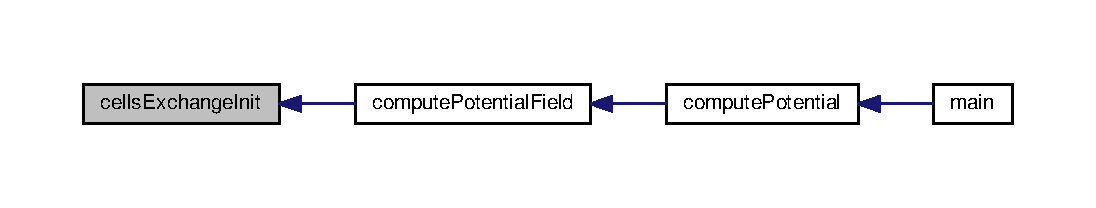
\includegraphics[width=350pt]{comm_8c_aa92fc6732720bc9accbbdef7fb02384f_icgraph}
\end{center}
\end{figure}


\hypertarget{comm_8c_ac5b7dbd1157ef088c4e6f8a9f08fcc4b}{\index{comm.\-c@{comm.\-c}!cells\-Exchange\-Wait@{cells\-Exchange\-Wait}}
\index{cells\-Exchange\-Wait@{cells\-Exchange\-Wait}!comm.c@{comm.\-c}}
\subsubsection[{cells\-Exchange\-Wait}]{\setlength{\rightskip}{0pt plus 5cm}void cells\-Exchange\-Wait (
\begin{DoxyParamCaption}
{}
\end{DoxyParamCaption}
)}}\label{comm_8c_ac5b7dbd1157ef088c4e6f8a9f08fcc4b}
This function waits for cells' data exchange completion. 

Definition at line 223 of file comm.\-c.



References lnc, M\-P\-Isize, nc, recv\-Count, req\-Recv, req\-Send, send\-Count, send\-Data, stop\-Run(), and tlnc.


\begin{DoxyCode}
224 \{
225   \textcolor{keywordtype}{int} i;
226   MPI\_Status status;
227 
228   \textcolor{keywordflow}{if} (\hyperlink{global_8h_a0845b4b004824f1fe3cd69db1672fa15}{nc} < \hyperlink{global_8h_a0d7d02544d01ceac87c9d5cadc3af0df}{MPIsize} || \hyperlink{global_8h_a0d7d02544d01ceac87c9d5cadc3af0df}{MPIsize} == 1)
229     \textcolor{keywordflow}{return};
230 
231   \textcolor{comment}{/* wait for send completion */}
232   \textcolor{keywordflow}{for} (i = 0; i < \hyperlink{global_8h_a0d7d02544d01ceac87c9d5cadc3af0df}{MPIsize}; i++) \{
233     \textcolor{keywordflow}{if} (\hyperlink{comm_8c_aed19f012b3fe7ae1966dcc8b89cdf7b2}{sendCount}[i] == 0 || \hyperlink{global_8h_ac3c96b975a3376c555ad22a7d2688b2f}{tlnc}[i] == 0 || \hyperlink{global_8h_a7065c019590815f10169c219f358e7d0}{lnc} == 0)
234       \textcolor{keywordflow}{continue};
235     \textcolor{keywordflow}{if} (MPI\_Wait(&\hyperlink{comm_8c_a827e028e778c94dd2e816ae6077a3198}{reqSend}[i], &status) != MPI\_SUCCESS)
236       \hyperlink{utils_8c_a07dd99a04f2723be164531a7a862fb67}{stopRun}(103, \textcolor{stringliteral}{"reqSend"}, \_\_FILE\_\_, \_\_LINE\_\_);
237   \}
238 
239   \textcolor{comment}{/* wait for receive completion */}
240   \textcolor{keywordflow}{for} (i = 0; i < \hyperlink{global_8h_a0d7d02544d01ceac87c9d5cadc3af0df}{MPIsize}; i++) \{
241     \textcolor{keywordflow}{if} (\hyperlink{comm_8c_a073b7079fe649b9ae1b5c4056ccaa4fb}{recvCount}[i] == 0 || \hyperlink{global_8h_ac3c96b975a3376c555ad22a7d2688b2f}{tlnc}[i] == 0 || \hyperlink{global_8h_a7065c019590815f10169c219f358e7d0}{lnc} == 0)
242       \textcolor{keywordflow}{continue};
243     \textcolor{keywordflow}{if} (MPI\_Wait(&\hyperlink{comm_8c_ad7a9f44424272a25979b199886bdce73}{reqRecv}[i], &status) != MPI\_SUCCESS)
244       \hyperlink{utils_8c_a07dd99a04f2723be164531a7a862fb67}{stopRun}(103, \textcolor{stringliteral}{"reqRecv"}, \_\_FILE\_\_, \_\_LINE\_\_);
245   \}
246 
247   \textcolor{comment}{/* some of the buffers can be deallocated here */}
248   free(\hyperlink{global_8h_ac928fbed09198ca6c116fb58a115b594}{sendData});
249   free(\hyperlink{comm_8c_a827e028e778c94dd2e816ae6077a3198}{reqSend});
250   free(\hyperlink{comm_8c_ad7a9f44424272a25979b199886bdce73}{reqRecv});
251 \}
\end{DoxyCode}


Here is the call graph for this function\-:\nopagebreak
\begin{figure}[H]
\begin{center}
\leavevmode
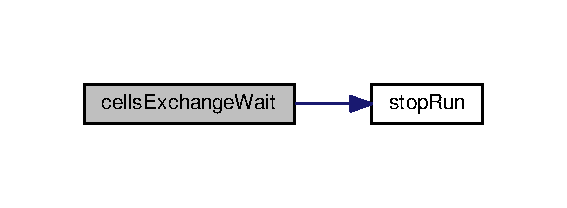
\includegraphics[width=272pt]{comm_8c_ac5b7dbd1157ef088c4e6f8a9f08fcc4b_cgraph}
\end{center}
\end{figure}




Here is the caller graph for this function\-:\nopagebreak
\begin{figure}[H]
\begin{center}
\leavevmode
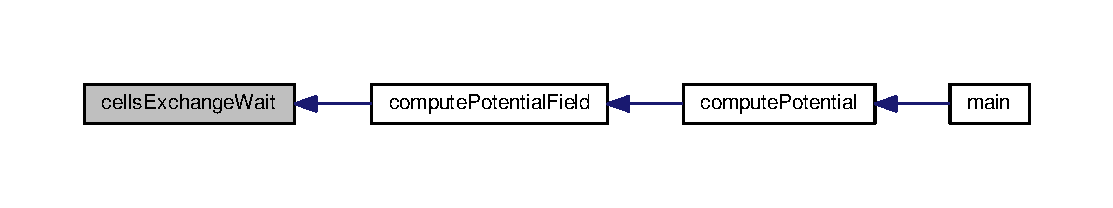
\includegraphics[width=350pt]{comm_8c_ac5b7dbd1157ef088c4e6f8a9f08fcc4b_icgraph}
\end{center}
\end{figure}


\hypertarget{comm_8c_a0a0b21ecf1a24a3cae73074d6bf6c68e}{\index{comm.\-c@{comm.\-c}!comm\-\_\-compare\-\_\-exp\-\_\-list@{comm\-\_\-compare\-\_\-exp\-\_\-list}}
\index{comm\-\_\-compare\-\_\-exp\-\_\-list@{comm\-\_\-compare\-\_\-exp\-\_\-list}!comm.c@{comm.\-c}}
\subsubsection[{comm\-\_\-compare\-\_\-exp\-\_\-list}]{\setlength{\rightskip}{0pt plus 5cm}int comm\-\_\-compare\-\_\-exp\-\_\-list (
\begin{DoxyParamCaption}
\item[{const void $\ast$}]{a, }
\item[{const void $\ast$}]{b}
\end{DoxyParamCaption}
)}}\label{comm_8c_a0a0b21ecf1a24a3cae73074d6bf6c68e}
This function is a comparison function used for sorting export list table. 

Definition at line 54 of file comm.\-c.


\begin{DoxyCode}
55 \{
56   \textcolor{keywordflow}{return} ((\textcolor{keyword}{struct} \hyperlink{structexpData}{expData} *) a)->proc - ((\textcolor{keyword}{struct }\hyperlink{structexpData}{expData} *) \hyperlink{tempf_8c_a74a523afdfebddf9b6b280e545977c5a}{b})->proc;
57 \}
\end{DoxyCode}


Here is the caller graph for this function\-:\nopagebreak
\begin{figure}[H]
\begin{center}
\leavevmode
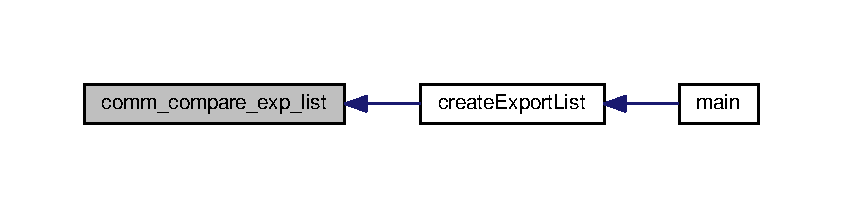
\includegraphics[width=350pt]{comm_8c_a0a0b21ecf1a24a3cae73074d6bf6c68e_icgraph}
\end{center}
\end{figure}


\hypertarget{comm_8c_abdd72f1d40c6c4bf47ad78c4f3c349d5}{\index{comm.\-c@{comm.\-c}!comm\-Cleanup@{comm\-Cleanup}}
\index{comm\-Cleanup@{comm\-Cleanup}!comm.c@{comm.\-c}}
\subsubsection[{comm\-Cleanup}]{\setlength{\rightskip}{0pt plus 5cm}void comm\-Cleanup (
\begin{DoxyParamCaption}
{}
\end{DoxyParamCaption}
)}}\label{comm_8c_abdd72f1d40c6c4bf47ad78c4f3c349d5}
This function deallocates all communication buffers and auxiliary tables. 

Definition at line 156 of file comm.\-c.



References M\-P\-Isize, nc, recv\-Count, recv\-Data, recv\-Dens\-Pot\-Data, recv\-Offset, send\-Count, and send\-Offset.


\begin{DoxyCode}
157 \{
158   \textcolor{keywordflow}{if} (\hyperlink{global_8h_a0845b4b004824f1fe3cd69db1672fa15}{nc} < \hyperlink{global_8h_a0d7d02544d01ceac87c9d5cadc3af0df}{MPIsize} || \hyperlink{global_8h_a0d7d02544d01ceac87c9d5cadc3af0df}{MPIsize} == 1)
159     \textcolor{keywordflow}{return};
160 
161   free(\hyperlink{global_8h_af851c922de87975e63161d38332d6a56}{recvData});
162   free(\hyperlink{global_8h_ac5932521dec6ac9c4208cb0312e002de}{recvDensPotData});
163 
164   free(\hyperlink{comm_8c_a6f7e234508139d1113a2f60a1b36c04a}{expList});
165 
166   free(\hyperlink{comm_8c_a073b7079fe649b9ae1b5c4056ccaa4fb}{recvCount});
167   free(\hyperlink{comm_8c_aed19f012b3fe7ae1966dcc8b89cdf7b2}{sendCount});
168 
169   free(\hyperlink{comm_8c_a16d801f1b7f6a598f31107a146b11f16}{sendOffset});
170   free(\hyperlink{comm_8c_a4f0cc30ef1f6185ba3d6406343e1a574}{recvOffset});
171 
172 \}
\end{DoxyCode}


Here is the caller graph for this function\-:\nopagebreak
\begin{figure}[H]
\begin{center}
\leavevmode
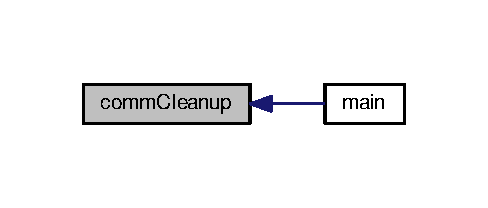
\includegraphics[width=234pt]{comm_8c_abdd72f1d40c6c4bf47ad78c4f3c349d5_icgraph}
\end{center}
\end{figure}


\hypertarget{comm_8c_a191bffd6b8283bf118dec0d0422fa2b3}{\index{comm.\-c@{comm.\-c}!create\-Export\-List@{create\-Export\-List}}
\index{create\-Export\-List@{create\-Export\-List}!comm.c@{comm.\-c}}
\subsubsection[{create\-Export\-List}]{\setlength{\rightskip}{0pt plus 5cm}void create\-Export\-List (
\begin{DoxyParamCaption}
{}
\end{DoxyParamCaption}
)}}\label{comm_8c_a191bffd6b8283bf118dec0d0422fa2b3}
This function uses Zoltan's library function Zoltan\-\_\-\-L\-B\-\_\-\-Box\-\_\-\-Assign to find possible intersections of cells' neighbourhoods and other processes' geometries. 

Definition at line 64 of file comm.\-c.



References exp\-Data\-::cell, cells, comm\-\_\-compare\-\_\-exp\-\_\-list(), h, cell\-Data\-::halo, lnc, M\-A\-X\-\_\-\-E\-X\-P\-O\-R\-T\-E\-D\-\_\-\-P\-E\-R\-\_\-\-P\-R\-O\-C, M\-P\-Irank, M\-P\-Isize, nc, num\-Exp, num\-Imp, exp\-Data\-::proc, recv\-Count, recv\-Offset, sdim, send\-Count, send\-Offset, stop\-Run(), tlnc, cell\-Data\-::x, cell\-Data\-::y, cell\-Data\-::z, and ztn.


\begin{DoxyCode}
65 \{
66 
67   \textcolor{keywordtype}{int} i, p;
68   \textcolor{keywordtype}{int} procs[\hyperlink{global_8h_a0d7d02544d01ceac87c9d5cadc3af0df}{MPIsize}];
69   \textcolor{keywordtype}{int} numprocs;
70 
71   \hyperlink{global_8h_a4c3c9a79704128f7fcc9ebf4bdd9e3fc}{numExp} = 0;
72   \hyperlink{global_8h_a6e7ffc829c0f608016617f9057885a9f}{numImp} = 0;
73   \textcolor{keywordflow}{if} (\hyperlink{global_8h_a0845b4b004824f1fe3cd69db1672fa15}{nc} < \hyperlink{global_8h_a0d7d02544d01ceac87c9d5cadc3af0df}{MPIsize} || \hyperlink{global_8h_a0d7d02544d01ceac87c9d5cadc3af0df}{MPIsize} == 1)
74     \textcolor{keywordflow}{return};
75 
76   \hyperlink{comm_8c_a6f7e234508139d1113a2f60a1b36c04a}{expList} =
77       (\textcolor{keyword}{struct }\hyperlink{structexpData}{expData} *) malloc(\textcolor{keyword}{sizeof}(\textcolor{keyword}{struct} \hyperlink{structexpData}{expData}) *
78                 \hyperlink{comm_8c_a93da5acfae81b763e797f8562d49ca64}{MAX\_EXPORTED\_PER\_PROC});
79   \hyperlink{comm_8c_a073b7079fe649b9ae1b5c4056ccaa4fb}{recvCount} = (\textcolor{keywordtype}{int} *) calloc(\hyperlink{global_8h_a0d7d02544d01ceac87c9d5cadc3af0df}{MPIsize}, \textcolor{keyword}{sizeof}(\textcolor{keywordtype}{int}));
80   \hyperlink{comm_8c_aed19f012b3fe7ae1966dcc8b89cdf7b2}{sendCount} = (\textcolor{keywordtype}{int} *) calloc(\hyperlink{global_8h_a0d7d02544d01ceac87c9d5cadc3af0df}{MPIsize}, \textcolor{keyword}{sizeof}(\textcolor{keywordtype}{int}));
81   \hyperlink{comm_8c_a16d801f1b7f6a598f31107a146b11f16}{sendOffset} = (int64\_t *) calloc(\hyperlink{global_8h_a0d7d02544d01ceac87c9d5cadc3af0df}{MPIsize}, \textcolor{keyword}{sizeof}(int64\_t));
82   \hyperlink{comm_8c_a4f0cc30ef1f6185ba3d6406343e1a574}{recvOffset} = (int64\_t *) calloc(\hyperlink{global_8h_a0d7d02544d01ceac87c9d5cadc3af0df}{MPIsize}, \textcolor{keyword}{sizeof}(int64\_t));
83 
84   \textcolor{comment}{/* loop over local cells */}
85   \textcolor{comment}{/*#pragma omp parallel for private(procs) */}
86   \textcolor{keywordflow}{for} (p = 0; p < \hyperlink{global_8h_a7065c019590815f10169c219f358e7d0}{lnc}; p++) \{
87     \textcolor{keywordtype}{double} xmin, xmax, ymin, ymax, zmin, zmax;
88     \textcolor{keywordtype}{double} r;
89 
90     \hyperlink{global_8h_a56da06a03aa369ca203be968cb56d16c}{cells}[p].\hyperlink{structcellData_a80ff3fcc4d03d0b1b01559839d12df5b}{halo} = 0;
91 
92     \textcolor{keywordflow}{if} (\hyperlink{global_8h_a0845b4b004824f1fe3cd69db1672fa15}{nc} < \hyperlink{global_8h_a0d7d02544d01ceac87c9d5cadc3af0df}{MPIsize})
93       \textcolor{keywordflow}{continue};
94 
95     r = \hyperlink{global_8h_a8ee9be1b5aa75abae556de3088cba6d9}{h} * 1.5;
96 
97     \textcolor{comment}{/* compute neighbourhood box */}
98     xmin = \hyperlink{global_8h_a56da06a03aa369ca203be968cb56d16c}{cells}[p].\hyperlink{structcellData_af88b946fb90d5f08b5fb740c70e98c10}{x} - r;
99     xmax = \hyperlink{global_8h_a56da06a03aa369ca203be968cb56d16c}{cells}[p].\hyperlink{structcellData_af88b946fb90d5f08b5fb740c70e98c10}{x} + r;
100     ymin = \hyperlink{global_8h_a56da06a03aa369ca203be968cb56d16c}{cells}[p].\hyperlink{structcellData_ab927965981178aa1fba979a37168db2a}{y} - r;
101     ymax = \hyperlink{global_8h_a56da06a03aa369ca203be968cb56d16c}{cells}[p].\hyperlink{structcellData_ab927965981178aa1fba979a37168db2a}{y} + r;
102     \textcolor{keywordflow}{if} (\hyperlink{global_8h_a2f8118c1bfdf986827e156210c33cbab}{sdim} == 3) \{
103       zmin = \hyperlink{global_8h_a56da06a03aa369ca203be968cb56d16c}{cells}[p].\hyperlink{structcellData_ab3e6ed577a7c669c19de1f9c1b46c872}{z} - r;
104       zmax = \hyperlink{global_8h_a56da06a03aa369ca203be968cb56d16c}{cells}[p].\hyperlink{structcellData_ab3e6ed577a7c669c19de1f9c1b46c872}{z} + r;
105     \} \textcolor{keywordflow}{else} \{
106       zmin = 0.0;
107       zmax = 0.0;
108     \}
109 
110     \textcolor{comment}{/* look for possible neighbours */}
111     Zoltan\_LB\_Box\_Assign(\hyperlink{global_8h_afc06c50b11f3b60d3738e669b612eb9c}{ztn}, xmin, ymin, zmin, xmax, ymax, zmax, procs,
112              &numprocs);
113 
114     \textcolor{comment}{/* loop over receivers */}
115     \textcolor{keywordflow}{for} (i = 0; i < numprocs; i++) \{
116       \textcolor{keywordflow}{if} (procs[i] == \hyperlink{global_8h_a710288ab7d2734acc4566a87a645325d}{MPIrank} || \hyperlink{global_8h_ac3c96b975a3376c555ad22a7d2688b2f}{tlnc}[procs[i]] == 0)
117     \textcolor{keywordflow}{continue};
118       \hyperlink{comm_8c_a6f7e234508139d1113a2f60a1b36c04a}{expList}[\hyperlink{global_8h_a4c3c9a79704128f7fcc9ebf4bdd9e3fc}{numExp}].\hyperlink{structexpData_af00601a22186810a9e6d16efb75862ce}{cell} = p;
119       \hyperlink{comm_8c_a6f7e234508139d1113a2f60a1b36c04a}{expList}[\hyperlink{global_8h_a4c3c9a79704128f7fcc9ebf4bdd9e3fc}{numExp}].\hyperlink{structexpData_a7e9d757c9982bd721d598bad366fbe62}{proc} = procs[i];
120       \hyperlink{global_8h_a56da06a03aa369ca203be968cb56d16c}{cells}[p].\hyperlink{structcellData_a80ff3fcc4d03d0b1b01559839d12df5b}{halo} = \hyperlink{global_8h_a710288ab7d2734acc4566a87a645325d}{MPIrank} + 1;
121       \hyperlink{comm_8c_aed19f012b3fe7ae1966dcc8b89cdf7b2}{sendCount}[procs[i]]++;
122       \hyperlink{global_8h_a4c3c9a79704128f7fcc9ebf4bdd9e3fc}{numExp}++;
123       \textcolor{comment}{/* upps! too many refugees */}
124       \textcolor{keywordflow}{if} (\hyperlink{global_8h_a4c3c9a79704128f7fcc9ebf4bdd9e3fc}{numExp} >= \hyperlink{comm_8c_a93da5acfae81b763e797f8562d49ca64}{MAX\_EXPORTED\_PER\_PROC})
125     \hyperlink{utils_8c_a07dd99a04f2723be164531a7a862fb67}{stopRun}(110, NULL, \_\_FILE\_\_, \_\_LINE\_\_);
126     \}
127   \}
128 
129   \textcolor{comment}{/* sort export list with respect to process number */}
130   qsort(\hyperlink{comm_8c_a6f7e234508139d1113a2f60a1b36c04a}{expList}, \hyperlink{global_8h_a4c3c9a79704128f7fcc9ebf4bdd9e3fc}{numExp}, \textcolor{keyword}{sizeof}(\textcolor{keyword}{struct} \hyperlink{structexpData}{expData}), 
      \hyperlink{comm_8c_a0a0b21ecf1a24a3cae73074d6bf6c68e}{comm\_compare\_exp\_list});
131 
132   \textcolor{comment}{/* distribute the information on transfer sizes between each process */}
133   MPI\_Alltoall(\hyperlink{comm_8c_aed19f012b3fe7ae1966dcc8b89cdf7b2}{sendCount}, 1, MPI\_INT, \hyperlink{comm_8c_a073b7079fe649b9ae1b5c4056ccaa4fb}{recvCount}, 1, MPI\_INT,
134            MPI\_COMM\_WORLD);
135 
136   \textcolor{comment}{/* compute send offsets */}
137   \hyperlink{comm_8c_a16d801f1b7f6a598f31107a146b11f16}{sendOffset}[0] = 0;
138   \textcolor{keywordflow}{for} (i = 1; i < \hyperlink{global_8h_a0d7d02544d01ceac87c9d5cadc3af0df}{MPIsize}; i++)
139     \hyperlink{comm_8c_a16d801f1b7f6a598f31107a146b11f16}{sendOffset}[i] = \hyperlink{comm_8c_a16d801f1b7f6a598f31107a146b11f16}{sendOffset}[i - 1] + \hyperlink{comm_8c_aed19f012b3fe7ae1966dcc8b89cdf7b2}{sendCount}[i - 1];
140 
141   \textcolor{comment}{/* compute receive offsets */}
142   \hyperlink{comm_8c_a4f0cc30ef1f6185ba3d6406343e1a574}{recvOffset}[0] = 0;
143   \textcolor{keywordflow}{for} (i = 1; i < \hyperlink{global_8h_a0d7d02544d01ceac87c9d5cadc3af0df}{MPIsize}; i++)
144     \hyperlink{comm_8c_a4f0cc30ef1f6185ba3d6406343e1a574}{recvOffset}[i] = \hyperlink{comm_8c_a4f0cc30ef1f6185ba3d6406343e1a574}{recvOffset}[i - 1] + \hyperlink{comm_8c_a073b7079fe649b9ae1b5c4056ccaa4fb}{recvCount}[i - 1];
145 
146   \textcolor{comment}{/* count cells to be imported */}
147   \textcolor{keywordflow}{for} (i = 0; i < \hyperlink{global_8h_a0d7d02544d01ceac87c9d5cadc3af0df}{MPIsize}; i++)
148     \hyperlink{global_8h_a6e7ffc829c0f608016617f9057885a9f}{numImp} += \hyperlink{comm_8c_a073b7079fe649b9ae1b5c4056ccaa4fb}{recvCount}[i];
149 
150 \}
\end{DoxyCode}


Here is the call graph for this function\-:\nopagebreak
\begin{figure}[H]
\begin{center}
\leavevmode
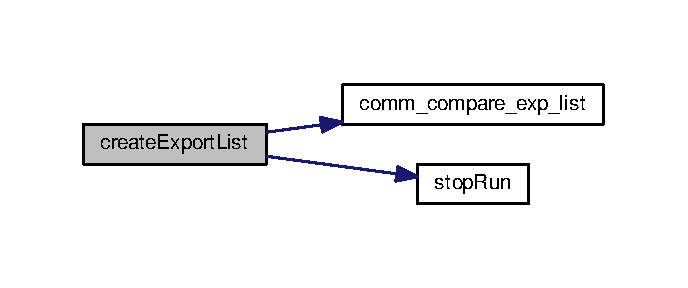
\includegraphics[width=330pt]{comm_8c_a191bffd6b8283bf118dec0d0422fa2b3_cgraph}
\end{center}
\end{figure}




Here is the caller graph for this function\-:\nopagebreak
\begin{figure}[H]
\begin{center}
\leavevmode
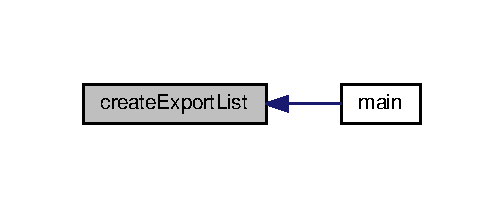
\includegraphics[width=242pt]{comm_8c_a191bffd6b8283bf118dec0d0422fa2b3_icgraph}
\end{center}
\end{figure}


\hypertarget{comm_8c_a206e073b7e35f281184b3487b3bbc055}{\index{comm.\-c@{comm.\-c}!dens\-Pot\-Exchange\-Init@{dens\-Pot\-Exchange\-Init}}
\index{dens\-Pot\-Exchange\-Init@{dens\-Pot\-Exchange\-Init}!comm.c@{comm.\-c}}
\subsubsection[{dens\-Pot\-Exchange\-Init}]{\setlength{\rightskip}{0pt plus 5cm}void dens\-Pot\-Exchange\-Init (
\begin{DoxyParamCaption}
{}
\end{DoxyParamCaption}
)}}\label{comm_8c_a206e073b7e35f281184b3487b3bbc055}
This function initiate sending and receiving density and potential values between processes. 

Definition at line 257 of file comm.\-c.



References exp\-Data\-::cell, cells, cell\-Data\-::density, dens\-Pot\-Data\-::density, lnc, M\-P\-Irank, M\-P\-Isize, nc, num\-Exp, num\-Imp, recv\-Count, recv\-Dens\-Pot\-Data, recv\-Offset, req\-Recv, req\-Send, send\-Count, send\-Dens\-Pot\-Data, send\-Offset, tlnc, cell\-Data\-::v, and dens\-Pot\-Data\-::v.


\begin{DoxyCode}
258 \{
259   \textcolor{keywordtype}{int} i;
260 
261   \textcolor{keywordflow}{if} (\hyperlink{global_8h_a0845b4b004824f1fe3cd69db1672fa15}{nc} < \hyperlink{global_8h_a0d7d02544d01ceac87c9d5cadc3af0df}{MPIsize} || \hyperlink{global_8h_a0d7d02544d01ceac87c9d5cadc3af0df}{MPIsize} == 1)
262     \textcolor{keywordflow}{return};
263 
264   \textcolor{comment}{/* allocate communication buffers */}
265   \hyperlink{global_8h_a5b0d78dc19924c0af131438356bfcdbd}{sendDensPotData} =
266       (\textcolor{keyword}{struct }\hyperlink{structdensPotData}{densPotData} *) malloc(\hyperlink{global_8h_a4c3c9a79704128f7fcc9ebf4bdd9e3fc}{numExp} * \textcolor{keyword}{sizeof}(\textcolor{keyword}{struct} 
      \hyperlink{structdensPotData}{densPotData}));
267   \hyperlink{global_8h_ac5932521dec6ac9c4208cb0312e002de}{recvDensPotData} =
268       (\textcolor{keyword}{struct }\hyperlink{structdensPotData}{densPotData} *) malloc(\hyperlink{global_8h_a6e7ffc829c0f608016617f9057885a9f}{numImp} * \textcolor{keyword}{sizeof}(\textcolor{keyword}{struct} 
      \hyperlink{structdensPotData}{densPotData}));
269   \hyperlink{comm_8c_a827e028e778c94dd2e816ae6077a3198}{reqSend} = (MPI\_Request *) malloc(\textcolor{keyword}{sizeof}(MPI\_Request) * \hyperlink{global_8h_a0d7d02544d01ceac87c9d5cadc3af0df}{MPIsize});
270   \hyperlink{comm_8c_ad7a9f44424272a25979b199886bdce73}{reqRecv} = (MPI\_Request *) malloc(\textcolor{keyword}{sizeof}(MPI\_Request) * \hyperlink{global_8h_a0d7d02544d01ceac87c9d5cadc3af0df}{MPIsize});
271 
272   \textcolor{comment}{/* create density and potential buffer for exporting */}
273   \textcolor{keywordflow}{for} (i = 0; i < \hyperlink{global_8h_a4c3c9a79704128f7fcc9ebf4bdd9e3fc}{numExp}; i++) \{
274     \hyperlink{global_8h_a5b0d78dc19924c0af131438356bfcdbd}{sendDensPotData}[i].\hyperlink{structdensPotData_a3b90d5a73541ab9402511d87bed076ef}{v} = \hyperlink{global_8h_a56da06a03aa369ca203be968cb56d16c}{cells}[\hyperlink{comm_8c_a6f7e234508139d1113a2f60a1b36c04a}{expList}[i].\hyperlink{structexpData_af00601a22186810a9e6d16efb75862ce}{cell}].
      \hyperlink{structcellData_a3b90d5a73541ab9402511d87bed076ef}{v};
275     \hyperlink{global_8h_a5b0d78dc19924c0af131438356bfcdbd}{sendDensPotData}[i].\hyperlink{structdensPotData_a6f8c052f8417728038991f7f2826d38d}{density} = \hyperlink{global_8h_a56da06a03aa369ca203be968cb56d16c}{cells}[\hyperlink{comm_8c_a6f7e234508139d1113a2f60a1b36c04a}{expList}[i].
      \hyperlink{structexpData_af00601a22186810a9e6d16efb75862ce}{cell}].\hyperlink{structcellData_a6f8c052f8417728038991f7f2826d38d}{density};
276   \}
277 
278   \textcolor{comment}{/* send data - asynchronous MPI call */}
279   \textcolor{keywordflow}{for} (i = 0; i < \hyperlink{global_8h_a0d7d02544d01ceac87c9d5cadc3af0df}{MPIsize}; i++) \{
280     \textcolor{keywordflow}{if} (\hyperlink{comm_8c_aed19f012b3fe7ae1966dcc8b89cdf7b2}{sendCount}[i] == 0 || \hyperlink{global_8h_ac3c96b975a3376c555ad22a7d2688b2f}{tlnc}[i] == 0 || \hyperlink{global_8h_a7065c019590815f10169c219f358e7d0}{lnc} == 0)
281       \textcolor{keywordflow}{continue};
282     MPI\_Isend(&\hyperlink{global_8h_a5b0d78dc19924c0af131438356bfcdbd}{sendDensPotData}[\hyperlink{comm_8c_a16d801f1b7f6a598f31107a146b11f16}{sendOffset}[i]],
283           \hyperlink{comm_8c_aed19f012b3fe7ae1966dcc8b89cdf7b2}{sendCount}[i] * \textcolor{keyword}{sizeof}(\textcolor{keyword}{struct} \hyperlink{structdensPotData}{densPotData}), MPI\_BYTE, i,
284           \hyperlink{global_8h_a710288ab7d2734acc4566a87a645325d}{MPIrank}, MPI\_COMM\_WORLD, &\hyperlink{comm_8c_a827e028e778c94dd2e816ae6077a3198}{reqSend}[i]);
285   \}
286 
287   \textcolor{comment}{/* receive data - asynchronous MPI call */}
288   \textcolor{keywordflow}{for} (i = 0; i < \hyperlink{global_8h_a0d7d02544d01ceac87c9d5cadc3af0df}{MPIsize}; i++) \{
289     \textcolor{keywordflow}{if} (\hyperlink{comm_8c_a073b7079fe649b9ae1b5c4056ccaa4fb}{recvCount}[i] == 0 || \hyperlink{global_8h_ac3c96b975a3376c555ad22a7d2688b2f}{tlnc}[i] == 0 || \hyperlink{global_8h_a7065c019590815f10169c219f358e7d0}{lnc} == 0)
290       \textcolor{keywordflow}{continue};
291     MPI\_Irecv(&\hyperlink{global_8h_ac5932521dec6ac9c4208cb0312e002de}{recvDensPotData}[\hyperlink{comm_8c_a4f0cc30ef1f6185ba3d6406343e1a574}{recvOffset}[i]],
292           \hyperlink{comm_8c_a073b7079fe649b9ae1b5c4056ccaa4fb}{recvCount}[i] * \textcolor{keyword}{sizeof}(\textcolor{keyword}{struct} \hyperlink{structdensPotData}{densPotData}), MPI\_BYTE, i, i,
293           MPI\_COMM\_WORLD, &\hyperlink{comm_8c_ad7a9f44424272a25979b199886bdce73}{reqRecv}[i]);
294   \}
295 
296 \}
\end{DoxyCode}


Here is the caller graph for this function\-:\nopagebreak
\begin{figure}[H]
\begin{center}
\leavevmode
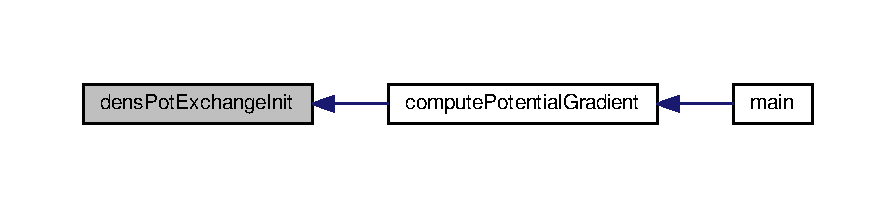
\includegraphics[width=350pt]{comm_8c_a206e073b7e35f281184b3487b3bbc055_icgraph}
\end{center}
\end{figure}


\hypertarget{comm_8c_afebf59220f4170178e5fb828d569aaab}{\index{comm.\-c@{comm.\-c}!dens\-Pot\-Exchange\-Wait@{dens\-Pot\-Exchange\-Wait}}
\index{dens\-Pot\-Exchange\-Wait@{dens\-Pot\-Exchange\-Wait}!comm.c@{comm.\-c}}
\subsubsection[{dens\-Pot\-Exchange\-Wait}]{\setlength{\rightskip}{0pt plus 5cm}void dens\-Pot\-Exchange\-Wait (
\begin{DoxyParamCaption}
{}
\end{DoxyParamCaption}
)}}\label{comm_8c_afebf59220f4170178e5fb828d569aaab}
This function waits for density and potential data exchange completion. 

Definition at line 301 of file comm.\-c.



References lnc, M\-P\-Isize, nc, recv\-Count, req\-Recv, req\-Send, send\-Count, send\-Dens\-Pot\-Data, stop\-Run(), and tlnc.


\begin{DoxyCode}
302 \{
303   \textcolor{keywordtype}{int} i;
304   MPI\_Status status;
305 
306   \textcolor{keywordflow}{if} (\hyperlink{global_8h_a0845b4b004824f1fe3cd69db1672fa15}{nc} < \hyperlink{global_8h_a0d7d02544d01ceac87c9d5cadc3af0df}{MPIsize} || \hyperlink{global_8h_a0d7d02544d01ceac87c9d5cadc3af0df}{MPIsize} == 1)
307     \textcolor{keywordflow}{return};
308 
309   \textcolor{comment}{// Wait for send completion}
310   \textcolor{keywordflow}{for} (i = 0; i < \hyperlink{global_8h_a0d7d02544d01ceac87c9d5cadc3af0df}{MPIsize}; i++) \{
311     \textcolor{keywordflow}{if} (\hyperlink{comm_8c_aed19f012b3fe7ae1966dcc8b89cdf7b2}{sendCount}[i] == 0 || \hyperlink{global_8h_ac3c96b975a3376c555ad22a7d2688b2f}{tlnc}[i] == 0 || \hyperlink{global_8h_a7065c019590815f10169c219f358e7d0}{lnc} == 0)
312       \textcolor{keywordflow}{continue};
313     \textcolor{keywordflow}{if} (MPI\_Wait(&\hyperlink{comm_8c_a827e028e778c94dd2e816ae6077a3198}{reqSend}[i], &status) != MPI\_SUCCESS)
314       \hyperlink{utils_8c_a07dd99a04f2723be164531a7a862fb67}{stopRun}(103, \textcolor{stringliteral}{"sending"}, \_\_FILE\_\_, \_\_LINE\_\_);
315   \}
316 
317   \textcolor{comment}{// Wait for receive completion}
318   \textcolor{keywordflow}{for} (i = 0; i < \hyperlink{global_8h_a0d7d02544d01ceac87c9d5cadc3af0df}{MPIsize}; i++) \{
319     \textcolor{keywordflow}{if} (\hyperlink{comm_8c_a073b7079fe649b9ae1b5c4056ccaa4fb}{recvCount}[i] == 0 || \hyperlink{global_8h_ac3c96b975a3376c555ad22a7d2688b2f}{tlnc}[i] == 0 || \hyperlink{global_8h_a7065c019590815f10169c219f358e7d0}{lnc} == 0)
320       \textcolor{keywordflow}{continue};
321     \textcolor{keywordflow}{if} (MPI\_Wait(&\hyperlink{comm_8c_ad7a9f44424272a25979b199886bdce73}{reqRecv}[i], &status) != MPI\_SUCCESS)
322       \hyperlink{utils_8c_a07dd99a04f2723be164531a7a862fb67}{stopRun}(103, \textcolor{stringliteral}{"receiving"}, \_\_FILE\_\_, \_\_LINE\_\_);
323   \}
324 
325   \textcolor{comment}{/* some of the buffers can be deallocated */}
326   free(\hyperlink{global_8h_a5b0d78dc19924c0af131438356bfcdbd}{sendDensPotData});
327   free(\hyperlink{comm_8c_a827e028e778c94dd2e816ae6077a3198}{reqSend});
328   free(\hyperlink{comm_8c_ad7a9f44424272a25979b199886bdce73}{reqRecv});
329 \}
\end{DoxyCode}


Here is the call graph for this function\-:\nopagebreak
\begin{figure}[H]
\begin{center}
\leavevmode
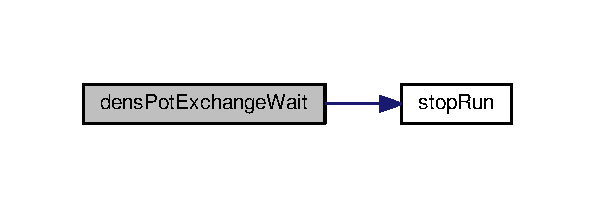
\includegraphics[width=286pt]{comm_8c_afebf59220f4170178e5fb828d569aaab_cgraph}
\end{center}
\end{figure}




Here is the caller graph for this function\-:\nopagebreak
\begin{figure}[H]
\begin{center}
\leavevmode
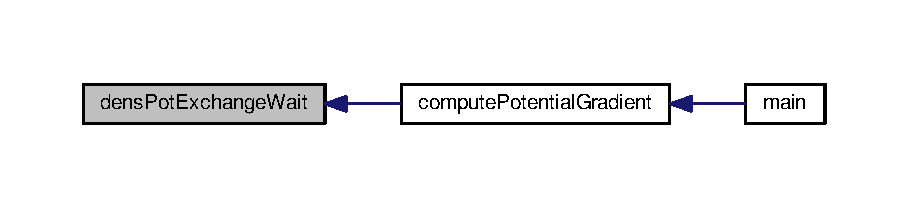
\includegraphics[width=350pt]{comm_8c_afebf59220f4170178e5fb828d569aaab_icgraph}
\end{center}
\end{figure}




\subsection{Variable Documentation}
\hypertarget{comm_8c_a6f7e234508139d1113a2f60a1b36c04a}{\index{comm.\-c@{comm.\-c}!exp\-List@{exp\-List}}
\index{exp\-List@{exp\-List}!comm.c@{comm.\-c}}
\subsubsection[{exp\-List}]{\setlength{\rightskip}{0pt plus 5cm}struct {\bf exp\-Data}$\ast$ exp\-List}}\label{comm_8c_a6f7e234508139d1113a2f60a1b36c04a}


Definition at line 43 of file comm.\-c.

\hypertarget{comm_8c_a073b7079fe649b9ae1b5c4056ccaa4fb}{\index{comm.\-c@{comm.\-c}!recv\-Count@{recv\-Count}}
\index{recv\-Count@{recv\-Count}!comm.c@{comm.\-c}}
\subsubsection[{recv\-Count}]{\setlength{\rightskip}{0pt plus 5cm}int$\ast$ recv\-Count}}\label{comm_8c_a073b7079fe649b9ae1b5c4056ccaa4fb}


Definition at line 45 of file comm.\-c.

\hypertarget{comm_8c_a4f0cc30ef1f6185ba3d6406343e1a574}{\index{comm.\-c@{comm.\-c}!recv\-Offset@{recv\-Offset}}
\index{recv\-Offset@{recv\-Offset}!comm.c@{comm.\-c}}
\subsubsection[{recv\-Offset}]{\setlength{\rightskip}{0pt plus 5cm}int64\-\_\-t$\ast$ recv\-Offset}}\label{comm_8c_a4f0cc30ef1f6185ba3d6406343e1a574}


Definition at line 41 of file comm.\-c.

\hypertarget{comm_8c_ad7a9f44424272a25979b199886bdce73}{\index{comm.\-c@{comm.\-c}!req\-Recv@{req\-Recv}}
\index{req\-Recv@{req\-Recv}!comm.c@{comm.\-c}}
\subsubsection[{req\-Recv}]{\setlength{\rightskip}{0pt plus 5cm}M\-P\-I\-\_\-\-Request$\ast$ req\-Recv}}\label{comm_8c_ad7a9f44424272a25979b199886bdce73}


Definition at line 38 of file comm.\-c.

\hypertarget{comm_8c_a827e028e778c94dd2e816ae6077a3198}{\index{comm.\-c@{comm.\-c}!req\-Send@{req\-Send}}
\index{req\-Send@{req\-Send}!comm.c@{comm.\-c}}
\subsubsection[{req\-Send}]{\setlength{\rightskip}{0pt plus 5cm}M\-P\-I\-\_\-\-Request$\ast$ req\-Send}}\label{comm_8c_a827e028e778c94dd2e816ae6077a3198}


Definition at line 37 of file comm.\-c.

\hypertarget{comm_8c_aed19f012b3fe7ae1966dcc8b89cdf7b2}{\index{comm.\-c@{comm.\-c}!send\-Count@{send\-Count}}
\index{send\-Count@{send\-Count}!comm.c@{comm.\-c}}
\subsubsection[{send\-Count}]{\setlength{\rightskip}{0pt plus 5cm}int$\ast$ send\-Count}}\label{comm_8c_aed19f012b3fe7ae1966dcc8b89cdf7b2}


Definition at line 46 of file comm.\-c.

\hypertarget{comm_8c_a16d801f1b7f6a598f31107a146b11f16}{\index{comm.\-c@{comm.\-c}!send\-Offset@{send\-Offset}}
\index{send\-Offset@{send\-Offset}!comm.c@{comm.\-c}}
\subsubsection[{send\-Offset}]{\setlength{\rightskip}{0pt plus 5cm}int64\-\_\-t$\ast$ send\-Offset}}\label{comm_8c_a16d801f1b7f6a598f31107a146b11f16}


Definition at line 40 of file comm.\-c.


\hypertarget{domdec_8c}{\section{domdec.\-c File Reference}
\label{domdec_8c}\index{domdec.\-c@{domdec.\-c}}
}


contains domain decomposition functions  


{\ttfamily \#include $<$stdio.\-h$>$}\\*
{\ttfamily \#include $<$stdlib.\-h$>$}\\*
{\ttfamily \#include \char`\"{}global.\-h\char`\"{}}\\*
Include dependency graph for domdec.\-c\-:\nopagebreak
\begin{figure}[H]
\begin{center}
\leavevmode
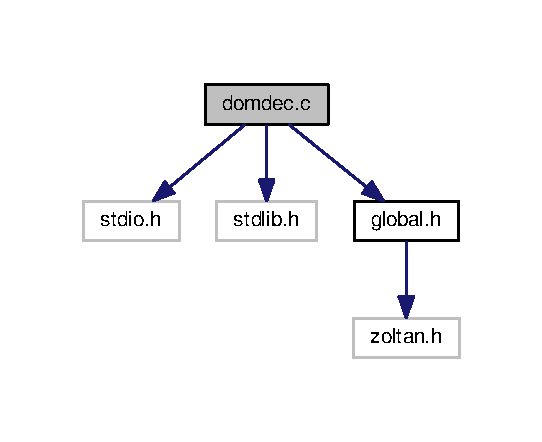
\includegraphics[width=260pt]{domdec_8c__incl}
\end{center}
\end{figure}
\subsection*{Functions}
\begin{DoxyCompactItemize}
\item 
int \hyperlink{domdec_8c_a646b3eaec99bfd258f4353ef2776d7eb}{ztn\-Return\-Dimension} (void $\ast$data, int $\ast$ierr)
\item 
void \hyperlink{domdec_8c_a5494b88a5d3049ebdaff2db552b62d88}{ztn\-Return\-Coords} (void $\ast$data, int \hyperlink{domdec_8c_a6c9a41a72d3fd2ab972e0ccfee7394ad}{num\-Gid\-Entries}, int \hyperlink{domdec_8c_ad836388e3004c88ef80be4e1cef479a5}{num\-Lid\-Entries}, Z\-O\-L\-T\-A\-N\-\_\-\-I\-D\-\_\-\-P\-T\-R global\-Id, Z\-O\-L\-T\-A\-N\-\_\-\-I\-D\-\_\-\-P\-T\-R local\-Id, double $\ast$geom\-Vec, int $\ast$ierr)
\item 
int \hyperlink{domdec_8c_ae16f55406fa663893e53bff6ec0d2891}{ztn\-Return\-Num\-Node} (void $\ast$data, int $\ast$ierr)
\item 
void \hyperlink{domdec_8c_afa9ccb22c460f072633a1033367a5da6}{ztn\-Return\-Owned\-Nodes} (void $\ast$data, int num\-G\-Id\-Entries, int num\-L\-Id\-Entries, Z\-O\-L\-T\-A\-N\-\_\-\-I\-D\-\_\-\-P\-T\-R global\-Ids, Z\-O\-L\-T\-A\-N\-\_\-\-I\-D\-\_\-\-P\-T\-R local\-Ids, int wgt\-Dim, float $\ast$obj\-Wgts, int $\ast$ierr)
\item 
int \hyperlink{domdec_8c_ae8ccac1e6575ca1ebe6ec4e9fde3625c}{ztn\-Return\-Particle\-Data\-Size} (void $\ast$data, int num\-G\-Id\-Entries, int num\-L\-Id\-Entries, Z\-O\-L\-T\-A\-N\-\_\-\-I\-D\-\_\-\-P\-T\-R global\-Id, Z\-O\-L\-T\-A\-N\-\_\-\-I\-D\-\_\-\-P\-T\-R local\-Id, int $\ast$ierr)
\item 
void \hyperlink{domdec_8c_a83bdab74033e8f1fb8a004c3f6a3b76c}{ztn\-Pack} (void $\ast$data, int num\-G\-Id\-Entries, int num\-L\-Id\-Entries, Z\-O\-L\-T\-A\-N\-\_\-\-I\-D\-\_\-\-P\-T\-R global\-Id, Z\-O\-L\-T\-A\-N\-\_\-\-I\-D\-\_\-\-P\-T\-R local\-Id, int dest, int size, char $\ast$buf, int $\ast$ierr)
\item 
void \hyperlink{domdec_8c_a7bb302f4a0beaad9c7c4f08162f1d66c}{ztn\-Pre} (void $\ast$data, int num\-G\-Id\-Entries, int num\-L\-Id\-Entries, int \hyperlink{domdec_8c_a63327cbfe51b3be8ccd7bd7947cf7768}{num\-Import}, Z\-O\-L\-T\-A\-N\-\_\-\-I\-D\-\_\-\-P\-T\-R import\-Global\-Ids, Z\-O\-L\-T\-A\-N\-\_\-\-I\-D\-\_\-\-P\-T\-R import\-Local\-Ids, int $\ast$\hyperlink{domdec_8c_aaf98961d02a34fd945de59d736ba66ce}{import\-Procs}, int $\ast$\hyperlink{domdec_8c_ac2fd1e8fdcde7633cb12cc36b7ffadc6}{import\-To\-Part}, int \hyperlink{domdec_8c_a71a7ca2f86ef16edaf1df524273e642a}{num\-Export}, Z\-O\-L\-T\-A\-N\-\_\-\-I\-D\-\_\-\-P\-T\-R export\-Global\-Ids, Z\-O\-L\-T\-A\-N\-\_\-\-I\-D\-\_\-\-P\-T\-R export\-Local\-Ids, int $\ast$\hyperlink{domdec_8c_a6992b2911e471d2452c8803e182fa4f1}{export\-Procs}, int $\ast$\hyperlink{domdec_8c_a51f5ba020bbcf6108262761504f19ed9}{export\-To\-Part}, int $\ast$ierr)
\item 
void \hyperlink{domdec_8c_aa46ced13f5fc202c3fcc841ff962a565}{ztn\-Mid} (void $\ast$data, int num\-G\-Id\-Entries, int num\-L\-Id\-Entries, int \hyperlink{domdec_8c_a63327cbfe51b3be8ccd7bd7947cf7768}{num\-Import}, Z\-O\-L\-T\-A\-N\-\_\-\-I\-D\-\_\-\-P\-T\-R import\-Global\-Ids, Z\-O\-L\-T\-A\-N\-\_\-\-I\-D\-\_\-\-P\-T\-R import\-Local\-Ids, int $\ast$\hyperlink{domdec_8c_aaf98961d02a34fd945de59d736ba66ce}{import\-Procs}, int $\ast$\hyperlink{domdec_8c_ac2fd1e8fdcde7633cb12cc36b7ffadc6}{import\-To\-Part}, int \hyperlink{domdec_8c_a71a7ca2f86ef16edaf1df524273e642a}{num\-Export}, Z\-O\-L\-T\-A\-N\-\_\-\-I\-D\-\_\-\-P\-T\-R export\-Global\-Ids, Z\-O\-L\-T\-A\-N\-\_\-\-I\-D\-\_\-\-P\-T\-R export\-Local\-Ids, int $\ast$\hyperlink{domdec_8c_a6992b2911e471d2452c8803e182fa4f1}{export\-Procs}, int $\ast$\hyperlink{domdec_8c_a51f5ba020bbcf6108262761504f19ed9}{export\-To\-Part}, int $\ast$ierr)
\item 
void \hyperlink{domdec_8c_a1e5da8ea3ac86aa8c5f131199f20e48d}{ztn\-Post} (void $\ast$data, int num\-G\-Id\-Entries, int num\-L\-Id\-Entries, int \hyperlink{domdec_8c_a63327cbfe51b3be8ccd7bd7947cf7768}{num\-Import}, Z\-O\-L\-T\-A\-N\-\_\-\-I\-D\-\_\-\-P\-T\-R import\-Global\-Ids, Z\-O\-L\-T\-A\-N\-\_\-\-I\-D\-\_\-\-P\-T\-R import\-Local\-Ids, int $\ast$\hyperlink{domdec_8c_aaf98961d02a34fd945de59d736ba66ce}{import\-Procs}, int $\ast$\hyperlink{domdec_8c_ac2fd1e8fdcde7633cb12cc36b7ffadc6}{import\-To\-Part}, int \hyperlink{domdec_8c_a71a7ca2f86ef16edaf1df524273e642a}{num\-Export}, Z\-O\-L\-T\-A\-N\-\_\-\-I\-D\-\_\-\-P\-T\-R export\-Global\-Ids, Z\-O\-L\-T\-A\-N\-\_\-\-I\-D\-\_\-\-P\-T\-R export\-Local\-Ids, int $\ast$\hyperlink{domdec_8c_a6992b2911e471d2452c8803e182fa4f1}{export\-Procs}, int $\ast$\hyperlink{domdec_8c_a51f5ba020bbcf6108262761504f19ed9}{export\-To\-Part}, int $\ast$ierr)
\item 
void \hyperlink{domdec_8c_aa2a71d2700b18abb4e381358df6967c5}{ztn\-Unpack} (void $\ast$data, int num\-G\-Id\-Entries, Z\-O\-L\-T\-A\-N\-\_\-\-I\-D\-\_\-\-P\-T\-R global\-Id, int size, char $\ast$buf, int $\ast$ierr)
\item 
void \hyperlink{domdec_8c_ae7429f968958e491ffc5aa144f564e0a}{decomposition\-Init} (int argc, char $\ast$$\ast$argv, M\-P\-I\-\_\-\-Comm Comm)
\item 
void \hyperlink{domdec_8c_aa62cb73f52f03ee27da62ae952212ceb}{decomposition\-Execute} ()
\item 
void \hyperlink{domdec_8c_a8dd9c084f2af53a06d1629e840f13ee8}{decomposition\-Finalize} ()
\end{DoxyCompactItemize}
\subsection*{Variables}
\begin{DoxyCompactItemize}
\item 
int \hyperlink{domdec_8c_a428798c15a127930411bd3af43e3cdc7}{changes}
\item 
int \hyperlink{domdec_8c_a6c9a41a72d3fd2ab972e0ccfee7394ad}{num\-Gid\-Entries}
\item 
int \hyperlink{domdec_8c_ad836388e3004c88ef80be4e1cef479a5}{num\-Lid\-Entries}
\item 
int \hyperlink{domdec_8c_a63327cbfe51b3be8ccd7bd7947cf7768}{num\-Import}
\item 
Z\-O\-L\-T\-A\-N\-\_\-\-I\-D\-\_\-\-P\-T\-R \hyperlink{domdec_8c_a7003e8d463d214680ced99e92a4e23c4}{import\-Global\-Gids}
\item 
Z\-O\-L\-T\-A\-N\-\_\-\-I\-D\-\_\-\-P\-T\-R \hyperlink{domdec_8c_a1ac001377defa550d2fe2627224ddb46}{import\-Local\-Gids}
\item 
int $\ast$ \hyperlink{domdec_8c_aaf98961d02a34fd945de59d736ba66ce}{import\-Procs}
\item 
int $\ast$ \hyperlink{domdec_8c_ac2fd1e8fdcde7633cb12cc36b7ffadc6}{import\-To\-Part}
\item 
int \hyperlink{domdec_8c_a71a7ca2f86ef16edaf1df524273e642a}{num\-Export}
\item 
Z\-O\-L\-T\-A\-N\-\_\-\-I\-D\-\_\-\-P\-T\-R \hyperlink{domdec_8c_ab47ca6ae0018cbdd0cdd75f8bbc1a1ca}{export\-Global\-Gids}
\item 
Z\-O\-L\-T\-A\-N\-\_\-\-I\-D\-\_\-\-P\-T\-R \hyperlink{domdec_8c_a5582bb1e54eaea68a6c2ddba7ab07553}{export\-Local\-Gids}
\item 
int $\ast$ \hyperlink{domdec_8c_a6992b2911e471d2452c8803e182fa4f1}{export\-Procs}
\item 
int $\ast$ \hyperlink{domdec_8c_a51f5ba020bbcf6108262761504f19ed9}{export\-To\-Part}
\end{DoxyCompactItemize}


\subsection{Detailed Description}
contains domain decomposition functions 

Definition in file \hyperlink{domdec_8c_source}{domdec.\-c}.



\subsection{Function Documentation}
\hypertarget{domdec_8c_aa62cb73f52f03ee27da62ae952212ceb}{\index{domdec.\-c@{domdec.\-c}!decomposition\-Execute@{decomposition\-Execute}}
\index{decomposition\-Execute@{decomposition\-Execute}!domdec.c@{domdec.\-c}}
\subsubsection[{decomposition\-Execute}]{\setlength{\rightskip}{0pt plus 5cm}void decomposition\-Execute (
\begin{DoxyParamCaption}
{}
\end{DoxyParamCaption}
)}}\label{domdec_8c_aa62cb73f52f03ee27da62ae952212ceb}
This function calls the Zoltan's domain decomposition and migration functions. It is called at the beginning of each simulation step. 

Definition at line 240 of file domdec.\-c.



References changes, export\-Global\-Gids, export\-Local\-Gids, export\-Procs, export\-To\-Part, import\-Global\-Gids, import\-Local\-Gids, import\-Procs, import\-To\-Part, M\-P\-Isize, nc, num\-Export, num\-Gid\-Entries, num\-Import, num\-Lid\-Entries, stop\-Run(), and ztn.


\begin{DoxyCode}
241 \{
242   \textcolor{keywordtype}{int} rc;
243   \textcolor{keywordtype}{int} i;
244 
245   \textcolor{keywordflow}{if} (\hyperlink{global_8h_a0845b4b004824f1fe3cd69db1672fa15}{nc} < \hyperlink{global_8h_a0d7d02544d01ceac87c9d5cadc3af0df}{MPIsize})
246     \textcolor{keywordflow}{return};
247 
248   rc = Zoltan\_LB\_Partition(\hyperlink{global_8h_afc06c50b11f3b60d3738e669b612eb9c}{ztn},  \textcolor{comment}{/* input (all remaining fields are output) */}
249                &\hyperlink{domdec_8c_a428798c15a127930411bd3af43e3cdc7}{changes}, \textcolor{comment}{/* 1 if partitioning was changed, 0 otherwise */}
250                &\hyperlink{domdec_8c_a6c9a41a72d3fd2ab972e0ccfee7394ad}{numGidEntries}, \textcolor{comment}{/* number of integers used for a global ID */}
251                &\hyperlink{domdec_8c_ad836388e3004c88ef80be4e1cef479a5}{numLidEntries}, \textcolor{comment}{/* number of integers used for a local ID */}
252                &\hyperlink{domdec_8c_a63327cbfe51b3be8ccd7bd7947cf7768}{numImport}, \textcolor{comment}{/* number of objects to be sent to me */}
253                &\hyperlink{domdec_8c_a7003e8d463d214680ced99e92a4e23c4}{importGlobalGids},   \textcolor{comment}{/* global IDs of objects to be sent to me */}
254                &\hyperlink{domdec_8c_a1ac001377defa550d2fe2627224ddb46}{importLocalGids}, \textcolor{comment}{/* local IDs of objects to be sent to me */}
255                &\hyperlink{domdec_8c_aaf98961d02a34fd945de59d736ba66ce}{importProcs}, \textcolor{comment}{/* process rank for source of each incoming object */}
256                &\hyperlink{domdec_8c_ac2fd1e8fdcde7633cb12cc36b7ffadc6}{importToPart},   \textcolor{comment}{/* new partition for each incoming object */}
257                &\hyperlink{domdec_8c_a71a7ca2f86ef16edaf1df524273e642a}{numExport}, \textcolor{comment}{/* number of objects I must send to other processes */}
258                &\hyperlink{domdec_8c_ab47ca6ae0018cbdd0cdd75f8bbc1a1ca}{exportGlobalGids},   \textcolor{comment}{/* global IDs of the objects I must send */}
259                &\hyperlink{domdec_8c_a5582bb1e54eaea68a6c2ddba7ab07553}{exportLocalGids}, \textcolor{comment}{/* local IDs of the objects I must send */}
260                &\hyperlink{domdec_8c_a6992b2911e471d2452c8803e182fa4f1}{exportProcs}, \textcolor{comment}{/* process to which I send each of the objects */}
261                &\hyperlink{domdec_8c_a51f5ba020bbcf6108262761504f19ed9}{exportToPart});  \textcolor{comment}{/* partition to which each object will belong */}
262 
263   \textcolor{keywordflow}{if} (rc != ZOLTAN\_OK)
264     \hyperlink{utils_8c_a07dd99a04f2723be164531a7a862fb67}{stopRun}(112, NULL, \_\_FILE\_\_, \_\_LINE\_\_);
265 
266   \textcolor{comment}{/* free the arrays allocated by Zoltan\_LB\_Partiotion */}
267   Zoltan\_LB\_Free\_Part(&\hyperlink{domdec_8c_a7003e8d463d214680ced99e92a4e23c4}{importGlobalGids}, &\hyperlink{domdec_8c_a1ac001377defa550d2fe2627224ddb46}{importLocalGids}, &
      \hyperlink{domdec_8c_aaf98961d02a34fd945de59d736ba66ce}{importProcs},
268               &\hyperlink{domdec_8c_ac2fd1e8fdcde7633cb12cc36b7ffadc6}{importToPart});
269   Zoltan\_LB\_Free\_Part(&\hyperlink{domdec_8c_ab47ca6ae0018cbdd0cdd75f8bbc1a1ca}{exportGlobalGids}, &\hyperlink{domdec_8c_a5582bb1e54eaea68a6c2ddba7ab07553}{exportLocalGids}, &
      \hyperlink{domdec_8c_a6992b2911e471d2452c8803e182fa4f1}{exportProcs},
270               &\hyperlink{domdec_8c_a51f5ba020bbcf6108262761504f19ed9}{exportToPart});
271 \}
\end{DoxyCode}


Here is the call graph for this function\-:\nopagebreak
\begin{figure}[H]
\begin{center}
\leavevmode
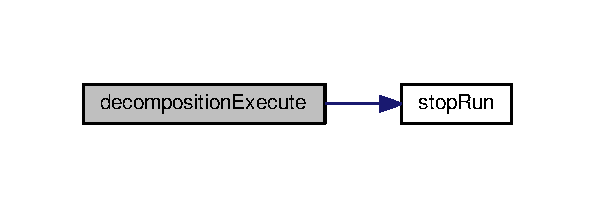
\includegraphics[width=286pt]{domdec_8c_aa62cb73f52f03ee27da62ae952212ceb_cgraph}
\end{center}
\end{figure}




Here is the caller graph for this function\-:\nopagebreak
\begin{figure}[H]
\begin{center}
\leavevmode
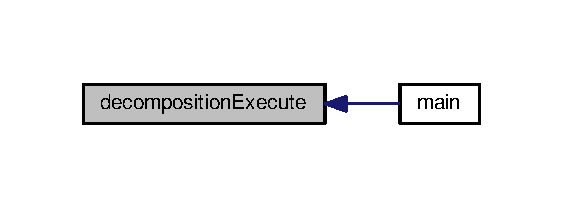
\includegraphics[width=270pt]{domdec_8c_aa62cb73f52f03ee27da62ae952212ceb_icgraph}
\end{center}
\end{figure}


\hypertarget{domdec_8c_a8dd9c084f2af53a06d1629e840f13ee8}{\index{domdec.\-c@{domdec.\-c}!decomposition\-Finalize@{decomposition\-Finalize}}
\index{decomposition\-Finalize@{decomposition\-Finalize}!domdec.c@{domdec.\-c}}
\subsubsection[{decomposition\-Finalize}]{\setlength{\rightskip}{0pt plus 5cm}void decomposition\-Finalize (
\begin{DoxyParamCaption}
{}
\end{DoxyParamCaption}
)}}\label{domdec_8c_a8dd9c084f2af53a06d1629e840f13ee8}
This function deactivates the Zoltan library. It is called at the end of the simulation. 

Definition at line 277 of file domdec.\-c.



References ztn.


\begin{DoxyCode}
278 \{
279   Zoltan\_Destroy(&\hyperlink{global_8h_afc06c50b11f3b60d3738e669b612eb9c}{ztn});
280 \}
\end{DoxyCode}


Here is the caller graph for this function\-:\nopagebreak
\begin{figure}[H]
\begin{center}
\leavevmode
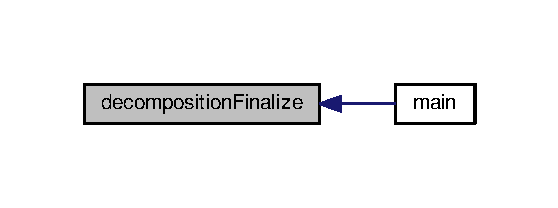
\includegraphics[width=268pt]{domdec_8c_a8dd9c084f2af53a06d1629e840f13ee8_icgraph}
\end{center}
\end{figure}


\hypertarget{domdec_8c_ae7429f968958e491ffc5aa144f564e0a}{\index{domdec.\-c@{domdec.\-c}!decomposition\-Init@{decomposition\-Init}}
\index{decomposition\-Init@{decomposition\-Init}!domdec.c@{domdec.\-c}}
\subsubsection[{decomposition\-Init}]{\setlength{\rightskip}{0pt plus 5cm}void decomposition\-Init (
\begin{DoxyParamCaption}
\item[{int}]{argc, }
\item[{char $\ast$$\ast$}]{argv, }
\item[{M\-P\-I\-\_\-\-Comm}]{Comm}
\end{DoxyParamCaption}
)}}\label{domdec_8c_ae7429f968958e491ffc5aa144f564e0a}
This function initializes the Zoltan library. It is called at the beginning of the simulation. 

Definition at line 191 of file domdec.\-c.



References cells, M\-P\-Irank, stop\-Run(), ztn, ztn\-Mid(), ztn\-Pack(), ztn\-Post(), ztn\-Pre(), ztn\-Return\-Coords(), ztn\-Return\-Dimension(), ztn\-Return\-Num\-Node(), ztn\-Return\-Owned\-Nodes(), ztn\-Return\-Particle\-Data\-Size(), and ztn\-Unpack().


\begin{DoxyCode}
192 \{
193   \textcolor{keywordtype}{int} rc;
194   \textcolor{keywordtype}{float} version;
195 
196   rc = Zoltan\_Initialize(argc, argv, &version);
197   \textcolor{keywordflow}{if} (rc != ZOLTAN\_OK)
198     \hyperlink{utils_8c_a07dd99a04f2723be164531a7a862fb67}{stopRun}(112, NULL, \_\_FILE\_\_, \_\_LINE\_\_);
199 
200   \textcolor{keywordflow}{if} (\hyperlink{global_8h_a710288ab7d2734acc4566a87a645325d}{MPIrank} == 0)
201     printf(\textcolor{stringliteral}{"Zoltan Version %.3f. Initialized.\(\backslash\)n"}, version);
202 
203   \hyperlink{global_8h_afc06c50b11f3b60d3738e669b612eb9c}{ztn} = Zoltan\_Create(MPI\_COMM\_WORLD);
204 
205   Zoltan\_Set\_Param(\hyperlink{global_8h_afc06c50b11f3b60d3738e669b612eb9c}{ztn}, \textcolor{stringliteral}{"IMBALANCE\_TOL"}, \textcolor{stringliteral}{"2.0"});
206   Zoltan\_Set\_Param(\hyperlink{global_8h_afc06c50b11f3b60d3738e669b612eb9c}{ztn}, \textcolor{stringliteral}{"LB\_METHOD"}, \textcolor{stringliteral}{"HSFC"});    \textcolor{comment}{/* Hilbert Space-Filling Curve Partitioning */}
207   Zoltan\_Set\_Param(\hyperlink{global_8h_afc06c50b11f3b60d3738e669b612eb9c}{ztn}, \textcolor{stringliteral}{"NUM\_GID\_ENTRIES"}, \textcolor{stringliteral}{"1"}); \textcolor{comment}{/* global ID is 1 integer */}
208   Zoltan\_Set\_Param(\hyperlink{global_8h_afc06c50b11f3b60d3738e669b612eb9c}{ztn}, \textcolor{stringliteral}{"NUM\_LID\_ENTRIES"}, \textcolor{stringliteral}{"1"}); \textcolor{comment}{/* local ID is 1 integer */}
209   Zoltan\_Set\_Param(\hyperlink{global_8h_afc06c50b11f3b60d3738e669b612eb9c}{ztn}, \textcolor{stringliteral}{"OBJ\_WEIGHT\_DIM"}, \textcolor{stringliteral}{"1"});  \textcolor{comment}{/* we use object weights */}
210   Zoltan\_Set\_Param(\hyperlink{global_8h_afc06c50b11f3b60d3738e669b612eb9c}{ztn}, \textcolor{stringliteral}{"DEBUG\_LEVEL"}, \textcolor{stringliteral}{"0"}); \textcolor{comment}{/* quiet mode; no output unless an error or warning is
       produced */}
211   Zoltan\_Set\_Param(\hyperlink{global_8h_afc06c50b11f3b60d3738e669b612eb9c}{ztn}, \textcolor{stringliteral}{"KEEP\_CUTS"}, \textcolor{stringliteral}{"1"});   \textcolor{comment}{/* save the cuts for later use */}
212   Zoltan\_Set\_Param(\hyperlink{global_8h_afc06c50b11f3b60d3738e669b612eb9c}{ztn}, \textcolor{stringliteral}{"AUTO\_MIGRATE"}, \textcolor{stringliteral}{"1"});    \textcolor{comment}{/* use the auto migration mechanism */}
213 
214   Zoltan\_Set\_Fn(\hyperlink{global_8h_afc06c50b11f3b60d3738e669b612eb9c}{ztn}, ZOLTAN\_NUM\_GEOM\_FN\_TYPE,
215         (\textcolor{keywordtype}{void} (*)()) \hyperlink{domdec_8c_a646b3eaec99bfd258f4353ef2776d7eb}{ztnReturnDimension}, \hyperlink{global_8h_a56da06a03aa369ca203be968cb56d16c}{cells});
216   Zoltan\_Set\_Fn(\hyperlink{global_8h_afc06c50b11f3b60d3738e669b612eb9c}{ztn}, ZOLTAN\_GEOM\_FN\_TYPE, (\textcolor{keywordtype}{void} (*)()) \hyperlink{domdec_8c_a5494b88a5d3049ebdaff2db552b62d88}{ztnReturnCoords},
217         \hyperlink{global_8h_a56da06a03aa369ca203be968cb56d16c}{cells});
218   Zoltan\_Set\_Fn(\hyperlink{global_8h_afc06c50b11f3b60d3738e669b612eb9c}{ztn}, ZOLTAN\_NUM\_OBJ\_FN\_TYPE, (\textcolor{keywordtype}{void} (*)()) \hyperlink{domdec_8c_ae16f55406fa663893e53bff6ec0d2891}{ztnReturnNumNode},
219         \hyperlink{global_8h_a56da06a03aa369ca203be968cb56d16c}{cells});
220   Zoltan\_Set\_Fn(\hyperlink{global_8h_afc06c50b11f3b60d3738e669b612eb9c}{ztn}, ZOLTAN\_OBJ\_LIST\_FN\_TYPE,
221         (\textcolor{keywordtype}{void} (*)()) \hyperlink{domdec_8c_afa9ccb22c460f072633a1033367a5da6}{ztnReturnOwnedNodes}, \hyperlink{global_8h_a56da06a03aa369ca203be968cb56d16c}{cells});
222   Zoltan\_Set\_Fn(\hyperlink{global_8h_afc06c50b11f3b60d3738e669b612eb9c}{ztn}, ZOLTAN\_OBJ\_SIZE\_FN\_TYPE,
223         (\textcolor{keywordtype}{void} (*)()) \hyperlink{domdec_8c_ae8ccac1e6575ca1ebe6ec4e9fde3625c}{ztnReturnParticleDataSize}, \hyperlink{global_8h_a56da06a03aa369ca203be968cb56d16c}{cells});
224   Zoltan\_Set\_Fn(\hyperlink{global_8h_afc06c50b11f3b60d3738e669b612eb9c}{ztn}, ZOLTAN\_PACK\_OBJ\_FN\_TYPE, (\textcolor{keywordtype}{void} (*)()) \hyperlink{domdec_8c_a83bdab74033e8f1fb8a004c3f6a3b76c}{ztnPack}, 
      \hyperlink{global_8h_a56da06a03aa369ca203be968cb56d16c}{cells});
225   Zoltan\_Set\_Fn(\hyperlink{global_8h_afc06c50b11f3b60d3738e669b612eb9c}{ztn}, ZOLTAN\_UNPACK\_OBJ\_FN\_TYPE, (\textcolor{keywordtype}{void} (*)()) \hyperlink{domdec_8c_aa2a71d2700b18abb4e381358df6967c5}{ztnUnpack},
226         \hyperlink{global_8h_a56da06a03aa369ca203be968cb56d16c}{cells});
227   Zoltan\_Set\_Fn(\hyperlink{global_8h_afc06c50b11f3b60d3738e669b612eb9c}{ztn}, ZOLTAN\_PRE\_MIGRATE\_PP\_FN\_TYPE, (\textcolor{keywordtype}{void} (*)()) \hyperlink{domdec_8c_a7bb302f4a0beaad9c7c4f08162f1d66c}{ztnPre},
228         \hyperlink{global_8h_a56da06a03aa369ca203be968cb56d16c}{cells});
229   Zoltan\_Set\_Fn(\hyperlink{global_8h_afc06c50b11f3b60d3738e669b612eb9c}{ztn}, ZOLTAN\_MID\_MIGRATE\_PP\_FN\_TYPE, (\textcolor{keywordtype}{void} (*)()) \hyperlink{domdec_8c_aa46ced13f5fc202c3fcc841ff962a565}{ztnMid},
230         \hyperlink{global_8h_a56da06a03aa369ca203be968cb56d16c}{cells});
231   Zoltan\_Set\_Fn(\hyperlink{global_8h_afc06c50b11f3b60d3738e669b612eb9c}{ztn}, ZOLTAN\_POST\_MIGRATE\_PP\_FN\_TYPE, (\textcolor{keywordtype}{void} (*)()) \hyperlink{domdec_8c_a1e5da8ea3ac86aa8c5f131199f20e48d}{ztnPost},
232         \hyperlink{global_8h_a56da06a03aa369ca203be968cb56d16c}{cells});
233 
234 \}
\end{DoxyCode}


Here is the call graph for this function\-:\nopagebreak
\begin{figure}[H]
\begin{center}
\leavevmode
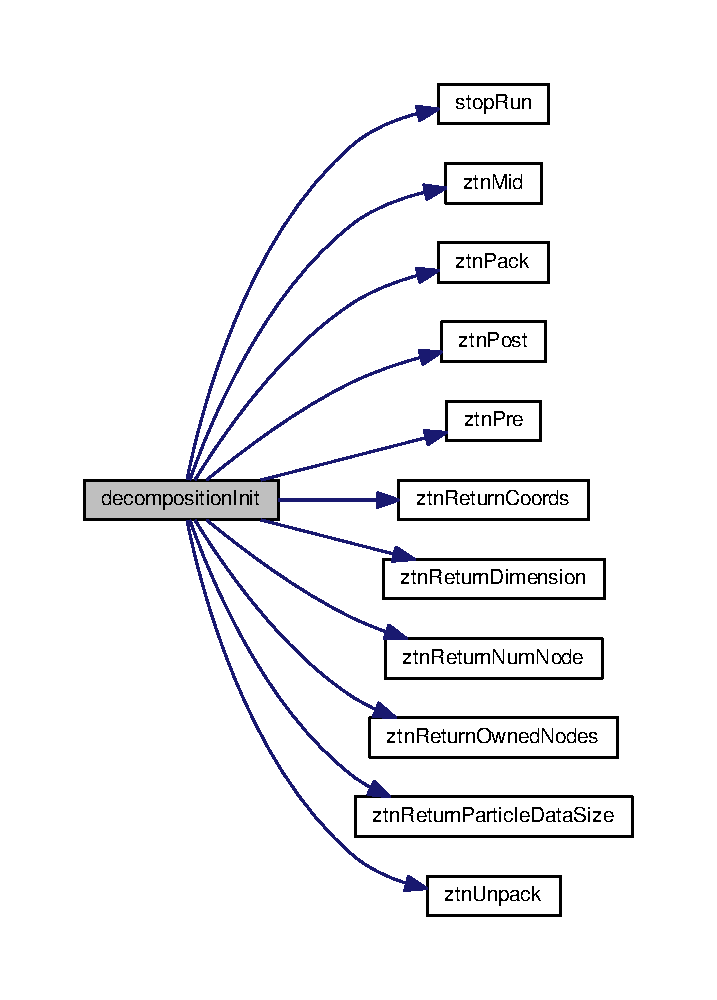
\includegraphics[width=344pt]{domdec_8c_ae7429f968958e491ffc5aa144f564e0a_cgraph}
\end{center}
\end{figure}




Here is the caller graph for this function\-:\nopagebreak
\begin{figure}[H]
\begin{center}
\leavevmode
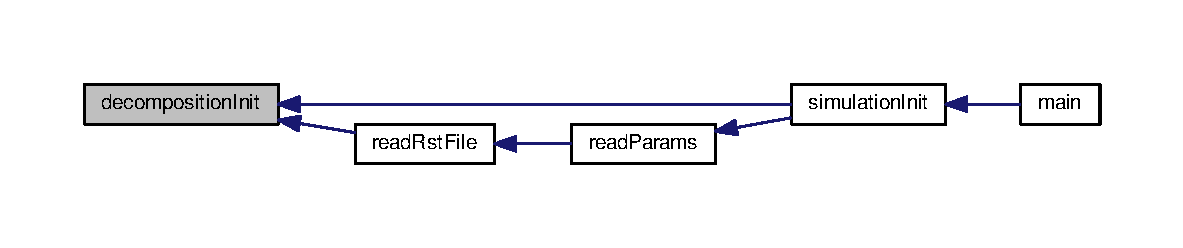
\includegraphics[width=350pt]{domdec_8c_ae7429f968958e491ffc5aa144f564e0a_icgraph}
\end{center}
\end{figure}


\hypertarget{domdec_8c_aa46ced13f5fc202c3fcc841ff962a565}{\index{domdec.\-c@{domdec.\-c}!ztn\-Mid@{ztn\-Mid}}
\index{ztn\-Mid@{ztn\-Mid}!domdec.c@{domdec.\-c}}
\subsubsection[{ztn\-Mid}]{\setlength{\rightskip}{0pt plus 5cm}void ztn\-Mid (
\begin{DoxyParamCaption}
\item[{void $\ast$}]{data, }
\item[{int}]{num\-G\-Id\-Entries, }
\item[{int}]{num\-L\-Id\-Entries, }
\item[{int}]{num\-Import, }
\item[{Z\-O\-L\-T\-A\-N\-\_\-\-I\-D\-\_\-\-P\-T\-R}]{import\-Global\-Ids, }
\item[{Z\-O\-L\-T\-A\-N\-\_\-\-I\-D\-\_\-\-P\-T\-R}]{import\-Local\-Ids, }
\item[{int $\ast$}]{import\-Procs, }
\item[{int $\ast$}]{import\-To\-Part, }
\item[{int}]{num\-Export, }
\item[{Z\-O\-L\-T\-A\-N\-\_\-\-I\-D\-\_\-\-P\-T\-R}]{export\-Global\-Ids, }
\item[{Z\-O\-L\-T\-A\-N\-\_\-\-I\-D\-\_\-\-P\-T\-R}]{export\-Local\-Ids, }
\item[{int $\ast$}]{export\-Procs, }
\item[{int $\ast$}]{export\-To\-Part, }
\item[{int $\ast$}]{ierr}
\end{DoxyParamCaption}
)}}\label{domdec_8c_aa46ced13f5fc202c3fcc841ff962a565}
Zoltan callback function. This function is executed after packing of send buffer and unpacking of receive buffer during migration. 

Definition at line 140 of file domdec.\-c.



References cell\-Data\-::gid, lnc, and num\-Export.


\begin{DoxyCode}
146 \{
147   \textcolor{keywordtype}{int} pos, i;
148   \textcolor{keyword}{struct }\hyperlink{structcellData}{cellData} *c = (\textcolor{keyword}{struct }\hyperlink{structcellData}{cellData} *) data;
149   pos = 0;
150   \textcolor{keywordflow}{for} (i = 0; i < \hyperlink{global_8h_a7065c019590815f10169c219f358e7d0}{lnc}; i++) \{
151     \textcolor{keywordflow}{if} (i != pos && c[i].\hyperlink{structcellData_abb4d4bd9231e9f994e87f32cc4fcfce8}{gid} != -1) \{
152       c[pos] = c[i];
153     \}
154     \textcolor{keywordflow}{if} (c[i].\hyperlink{structcellData_abb4d4bd9231e9f994e87f32cc4fcfce8}{gid} != -1)
155       pos++;
156   \}
157   lnc = lnc - \hyperlink{domdec_8c_a71a7ca2f86ef16edaf1df524273e642a}{numExport};
158 \}
\end{DoxyCode}


Here is the caller graph for this function\-:\nopagebreak
\begin{figure}[H]
\begin{center}
\leavevmode
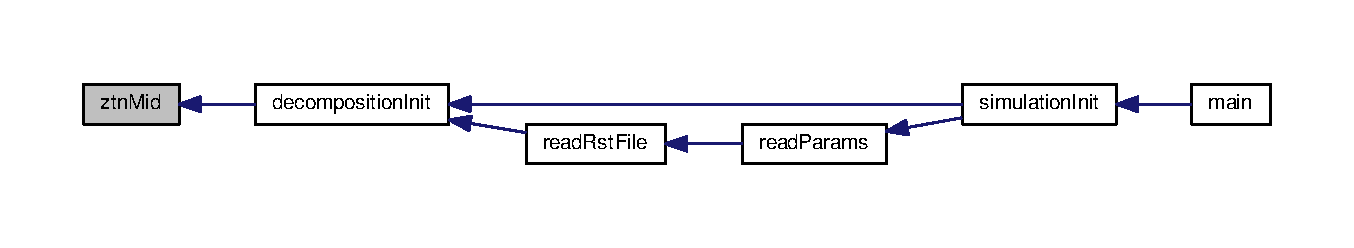
\includegraphics[width=350pt]{domdec_8c_aa46ced13f5fc202c3fcc841ff962a565_icgraph}
\end{center}
\end{figure}


\hypertarget{domdec_8c_a83bdab74033e8f1fb8a004c3f6a3b76c}{\index{domdec.\-c@{domdec.\-c}!ztn\-Pack@{ztn\-Pack}}
\index{ztn\-Pack@{ztn\-Pack}!domdec.c@{domdec.\-c}}
\subsubsection[{ztn\-Pack}]{\setlength{\rightskip}{0pt plus 5cm}void ztn\-Pack (
\begin{DoxyParamCaption}
\item[{void $\ast$}]{data, }
\item[{int}]{num\-G\-Id\-Entries, }
\item[{int}]{num\-L\-Id\-Entries, }
\item[{Z\-O\-L\-T\-A\-N\-\_\-\-I\-D\-\_\-\-P\-T\-R}]{global\-Id, }
\item[{Z\-O\-L\-T\-A\-N\-\_\-\-I\-D\-\_\-\-P\-T\-R}]{local\-Id, }
\item[{int}]{dest, }
\item[{int}]{size, }
\item[{char $\ast$}]{buf, }
\item[{int $\ast$}]{ierr}
\end{DoxyParamCaption}
)}}\label{domdec_8c_a83bdab74033e8f1fb8a004c3f6a3b76c}
Zoltan callback function. This function packs data into a send buffer before migration. 

Definition at line 115 of file domdec.\-c.



References cell\-Data\-::gid.


\begin{DoxyCode}
118 \{
119   \textcolor{keyword}{struct }\hyperlink{structcellData}{cellData} *c = (\textcolor{keyword}{struct }\hyperlink{structcellData}{cellData} *) data;
120   memcpy(buf, &(c[localId[0]]), \textcolor{keyword}{sizeof}(\textcolor{keyword}{struct} \hyperlink{structcellData}{cellData}));
121   c[(int) (*localId)].\hyperlink{structcellData_abb4d4bd9231e9f994e87f32cc4fcfce8}{gid} = -1;  \textcolor{comment}{/* mark local particle as exported */}
122 \}
\end{DoxyCode}


Here is the caller graph for this function\-:\nopagebreak
\begin{figure}[H]
\begin{center}
\leavevmode
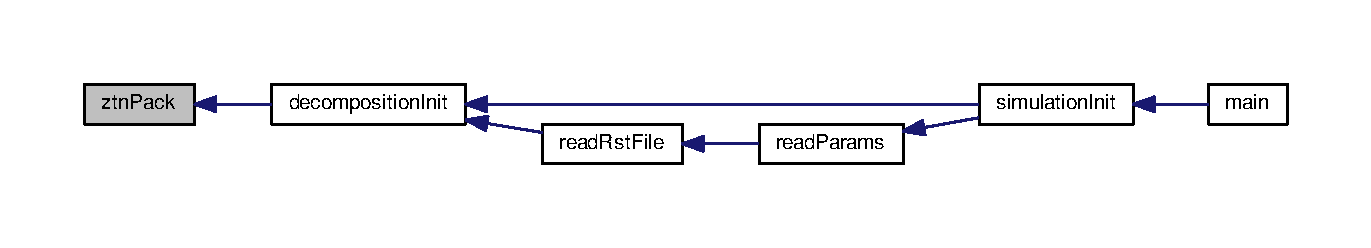
\includegraphics[width=350pt]{domdec_8c_a83bdab74033e8f1fb8a004c3f6a3b76c_icgraph}
\end{center}
\end{figure}


\hypertarget{domdec_8c_a1e5da8ea3ac86aa8c5f131199f20e48d}{\index{domdec.\-c@{domdec.\-c}!ztn\-Post@{ztn\-Post}}
\index{ztn\-Post@{ztn\-Post}!domdec.c@{domdec.\-c}}
\subsubsection[{ztn\-Post}]{\setlength{\rightskip}{0pt plus 5cm}void ztn\-Post (
\begin{DoxyParamCaption}
\item[{void $\ast$}]{data, }
\item[{int}]{num\-G\-Id\-Entries, }
\item[{int}]{num\-L\-Id\-Entries, }
\item[{int}]{num\-Import, }
\item[{Z\-O\-L\-T\-A\-N\-\_\-\-I\-D\-\_\-\-P\-T\-R}]{import\-Global\-Ids, }
\item[{Z\-O\-L\-T\-A\-N\-\_\-\-I\-D\-\_\-\-P\-T\-R}]{import\-Local\-Ids, }
\item[{int $\ast$}]{import\-Procs, }
\item[{int $\ast$}]{import\-To\-Part, }
\item[{int}]{num\-Export, }
\item[{Z\-O\-L\-T\-A\-N\-\_\-\-I\-D\-\_\-\-P\-T\-R}]{export\-Global\-Ids, }
\item[{Z\-O\-L\-T\-A\-N\-\_\-\-I\-D\-\_\-\-P\-T\-R}]{export\-Local\-Ids, }
\item[{int $\ast$}]{export\-Procs, }
\item[{int $\ast$}]{export\-To\-Part, }
\item[{int $\ast$}]{ierr}
\end{DoxyParamCaption}
)}}\label{domdec_8c_a1e5da8ea3ac86aa8c5f131199f20e48d}
Zoltan callback function. This function is executed after migration of data between processes. 

Definition at line 163 of file domdec.\-c.



References lnc, and tlnc.


\begin{DoxyCode}
169 \{
170   \textcolor{comment}{/* any post communication operations should go here */}
171   \textcolor{comment}{/* gather number of cells from each process */}
172   MPI\_Allgather(&\hyperlink{global_8h_a7065c019590815f10169c219f358e7d0}{lnc}, 1, MPI\_LONG\_LONG, \hyperlink{global_8h_ac3c96b975a3376c555ad22a7d2688b2f}{tlnc}, 1, MPI\_LONG\_LONG,
173         MPI\_COMM\_WORLD);
174 \}
\end{DoxyCode}


Here is the caller graph for this function\-:\nopagebreak
\begin{figure}[H]
\begin{center}
\leavevmode
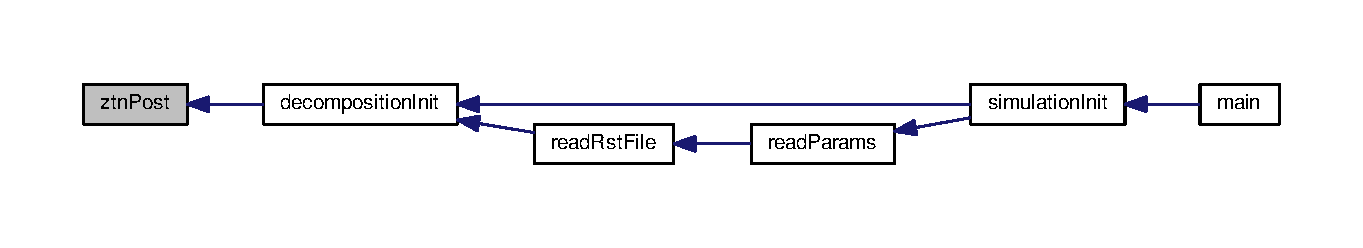
\includegraphics[width=350pt]{domdec_8c_a1e5da8ea3ac86aa8c5f131199f20e48d_icgraph}
\end{center}
\end{figure}


\hypertarget{domdec_8c_a7bb302f4a0beaad9c7c4f08162f1d66c}{\index{domdec.\-c@{domdec.\-c}!ztn\-Pre@{ztn\-Pre}}
\index{ztn\-Pre@{ztn\-Pre}!domdec.c@{domdec.\-c}}
\subsubsection[{ztn\-Pre}]{\setlength{\rightskip}{0pt plus 5cm}void ztn\-Pre (
\begin{DoxyParamCaption}
\item[{void $\ast$}]{data, }
\item[{int}]{num\-G\-Id\-Entries, }
\item[{int}]{num\-L\-Id\-Entries, }
\item[{int}]{num\-Import, }
\item[{Z\-O\-L\-T\-A\-N\-\_\-\-I\-D\-\_\-\-P\-T\-R}]{import\-Global\-Ids, }
\item[{Z\-O\-L\-T\-A\-N\-\_\-\-I\-D\-\_\-\-P\-T\-R}]{import\-Local\-Ids, }
\item[{int $\ast$}]{import\-Procs, }
\item[{int $\ast$}]{import\-To\-Part, }
\item[{int}]{num\-Export, }
\item[{Z\-O\-L\-T\-A\-N\-\_\-\-I\-D\-\_\-\-P\-T\-R}]{export\-Global\-Ids, }
\item[{Z\-O\-L\-T\-A\-N\-\_\-\-I\-D\-\_\-\-P\-T\-R}]{export\-Local\-Ids, }
\item[{int $\ast$}]{export\-Procs, }
\item[{int $\ast$}]{export\-To\-Part, }
\item[{int $\ast$}]{ierr}
\end{DoxyParamCaption}
)}}\label{domdec_8c_a7bb302f4a0beaad9c7c4f08162f1d66c}
Zoltan callback function. This function is executed before migration of data between processes. 

Definition at line 127 of file domdec.\-c.


\begin{DoxyCode}
133 \{
134   \textcolor{comment}{/* any pre communication operations should go here */}
135 \}
\end{DoxyCode}


Here is the caller graph for this function\-:\nopagebreak
\begin{figure}[H]
\begin{center}
\leavevmode
\includegraphics[width=350pt]{domdec_8c_a7bb302f4a0beaad9c7c4f08162f1d66c_icgraph}
\end{center}
\end{figure}


\hypertarget{domdec_8c_a5494b88a5d3049ebdaff2db552b62d88}{\index{domdec.\-c@{domdec.\-c}!ztn\-Return\-Coords@{ztn\-Return\-Coords}}
\index{ztn\-Return\-Coords@{ztn\-Return\-Coords}!domdec.c@{domdec.\-c}}
\subsubsection[{ztn\-Return\-Coords}]{\setlength{\rightskip}{0pt plus 5cm}void ztn\-Return\-Coords (
\begin{DoxyParamCaption}
\item[{void $\ast$}]{data, }
\item[{int}]{num\-Gid\-Entries, }
\item[{int}]{num\-Lid\-Entries, }
\item[{Z\-O\-L\-T\-A\-N\-\_\-\-I\-D\-\_\-\-P\-T\-R}]{global\-Id, }
\item[{Z\-O\-L\-T\-A\-N\-\_\-\-I\-D\-\_\-\-P\-T\-R}]{local\-Id, }
\item[{double $\ast$}]{geom\-Vec, }
\item[{int $\ast$}]{ierr}
\end{DoxyParamCaption}
)}}\label{domdec_8c_a5494b88a5d3049ebdaff2db552b62d88}
Zoltan callback function. This function returns the spatial coordinates of the cell identified by its global and local id. 

Definition at line 61 of file domdec.\-c.



References cells, sdim, cell\-Data\-::x, cell\-Data\-::y, and cell\-Data\-::z.


\begin{DoxyCode}
64 \{
65   \textcolor{keywordflow}{if} (\hyperlink{global_8h_a2f8118c1bfdf986827e156210c33cbab}{sdim} == 3) \{
66     geomVec[0] = \hyperlink{global_8h_a56da06a03aa369ca203be968cb56d16c}{cells}[localId[0]].\hyperlink{structcellData_af88b946fb90d5f08b5fb740c70e98c10}{x};
67     geomVec[1] = \hyperlink{global_8h_a56da06a03aa369ca203be968cb56d16c}{cells}[localId[0]].\hyperlink{structcellData_ab927965981178aa1fba979a37168db2a}{y};
68     geomVec[2] = \hyperlink{global_8h_a56da06a03aa369ca203be968cb56d16c}{cells}[localId[0]].\hyperlink{structcellData_ab3e6ed577a7c669c19de1f9c1b46c872}{z};
69   \}
70   \textcolor{keywordflow}{if} (\hyperlink{global_8h_a2f8118c1bfdf986827e156210c33cbab}{sdim} == 2) \{
71     geomVec[0] = \hyperlink{global_8h_a56da06a03aa369ca203be968cb56d16c}{cells}[localId[0]].\hyperlink{structcellData_af88b946fb90d5f08b5fb740c70e98c10}{x};
72     geomVec[1] = \hyperlink{global_8h_a56da06a03aa369ca203be968cb56d16c}{cells}[localId[0]].\hyperlink{structcellData_ab927965981178aa1fba979a37168db2a}{y};
73   \}
74 \}
\end{DoxyCode}


Here is the caller graph for this function\-:\nopagebreak
\begin{figure}[H]
\begin{center}
\leavevmode
\includegraphics[width=350pt]{domdec_8c_a5494b88a5d3049ebdaff2db552b62d88_icgraph}
\end{center}
\end{figure}


\hypertarget{domdec_8c_a646b3eaec99bfd258f4353ef2776d7eb}{\index{domdec.\-c@{domdec.\-c}!ztn\-Return\-Dimension@{ztn\-Return\-Dimension}}
\index{ztn\-Return\-Dimension@{ztn\-Return\-Dimension}!domdec.c@{domdec.\-c}}
\subsubsection[{ztn\-Return\-Dimension}]{\setlength{\rightskip}{0pt plus 5cm}int ztn\-Return\-Dimension (
\begin{DoxyParamCaption}
\item[{void $\ast$}]{data, }
\item[{int $\ast$}]{ierr}
\end{DoxyParamCaption}
)}}\label{domdec_8c_a646b3eaec99bfd258f4353ef2776d7eb}
Zoltan callback function. This function returns the dimension (2\-D or 3\-D) of the system. 

Definition at line 50 of file domdec.\-c.



References sdim.


\begin{DoxyCode}
51 \{
52   \textcolor{keywordflow}{if} (\hyperlink{global_8h_a2f8118c1bfdf986827e156210c33cbab}{sdim} == 3)
53     \textcolor{keywordflow}{return} 3;
54   \textcolor{keywordflow}{if} (\hyperlink{global_8h_a2f8118c1bfdf986827e156210c33cbab}{sdim} == 2)
55     \textcolor{keywordflow}{return} 2;
56 \}
\end{DoxyCode}


Here is the caller graph for this function\-:\nopagebreak
\begin{figure}[H]
\begin{center}
\leavevmode
\includegraphics[width=350pt]{domdec_8c_a646b3eaec99bfd258f4353ef2776d7eb_icgraph}
\end{center}
\end{figure}


\hypertarget{domdec_8c_ae16f55406fa663893e53bff6ec0d2891}{\index{domdec.\-c@{domdec.\-c}!ztn\-Return\-Num\-Node@{ztn\-Return\-Num\-Node}}
\index{ztn\-Return\-Num\-Node@{ztn\-Return\-Num\-Node}!domdec.c@{domdec.\-c}}
\subsubsection[{ztn\-Return\-Num\-Node}]{\setlength{\rightskip}{0pt plus 5cm}int ztn\-Return\-Num\-Node (
\begin{DoxyParamCaption}
\item[{void $\ast$}]{data, }
\item[{int $\ast$}]{ierr}
\end{DoxyParamCaption}
)}}\label{domdec_8c_ae16f55406fa663893e53bff6ec0d2891}
Zoltan callback function. This function returns the number of cells assigned to this process. 

Definition at line 79 of file domdec.\-c.



References lnc.


\begin{DoxyCode}
80 \{
81   \textcolor{keywordflow}{return} \hyperlink{global_8h_a7065c019590815f10169c219f358e7d0}{lnc};
82 \}
\end{DoxyCode}


Here is the caller graph for this function\-:\nopagebreak
\begin{figure}[H]
\begin{center}
\leavevmode
\includegraphics[width=350pt]{domdec_8c_ae16f55406fa663893e53bff6ec0d2891_icgraph}
\end{center}
\end{figure}


\hypertarget{domdec_8c_afa9ccb22c460f072633a1033367a5da6}{\index{domdec.\-c@{domdec.\-c}!ztn\-Return\-Owned\-Nodes@{ztn\-Return\-Owned\-Nodes}}
\index{ztn\-Return\-Owned\-Nodes@{ztn\-Return\-Owned\-Nodes}!domdec.c@{domdec.\-c}}
\subsubsection[{ztn\-Return\-Owned\-Nodes}]{\setlength{\rightskip}{0pt plus 5cm}void ztn\-Return\-Owned\-Nodes (
\begin{DoxyParamCaption}
\item[{void $\ast$}]{data, }
\item[{int}]{num\-G\-Id\-Entries, }
\item[{int}]{num\-L\-Id\-Entries, }
\item[{Z\-O\-L\-T\-A\-N\-\_\-\-I\-D\-\_\-\-P\-T\-R}]{global\-Ids, }
\item[{Z\-O\-L\-T\-A\-N\-\_\-\-I\-D\-\_\-\-P\-T\-R}]{local\-Ids, }
\item[{int}]{wgt\-Dim, }
\item[{float $\ast$}]{obj\-Wgts, }
\item[{int $\ast$}]{ierr}
\end{DoxyParamCaption}
)}}\label{domdec_8c_afa9ccb22c460f072633a1033367a5da6}
Zoltan callback function. This function fills the tables of global ids, local ids and weights for all cells assigned to this process. 

Definition at line 87 of file domdec.\-c.



References cells, cell\-Data\-::gid, and lnc.


\begin{DoxyCode}
90 \{
91   \textcolor{keywordtype}{int} i;
92   \textcolor{keyword}{struct }cell *p = (\textcolor{keyword}{struct }cell *) data;
93   \textcolor{keywordflow}{for} (i = 0; i < \hyperlink{global_8h_a7065c019590815f10169c219f358e7d0}{lnc}; i++) \{
94     globalIds[i * numGIdEntries] = \hyperlink{global_8h_a56da06a03aa369ca203be968cb56d16c}{cells}[i].\hyperlink{structcellData_abb4d4bd9231e9f994e87f32cc4fcfce8}{gid};
95     localIds[i * numLIdEntries] = i;
96     objWgts[i] = 1.0;
97     \textcolor{comment}{//if(nc==1 || step==0) obj\_wgts[i]=1.0;}
98     \textcolor{comment}{//else obj\_wgts[i]=cells[i].density;}
99   \}
100 \}
\end{DoxyCode}


Here is the caller graph for this function\-:\nopagebreak
\begin{figure}[H]
\begin{center}
\leavevmode
\includegraphics[width=350pt]{domdec_8c_afa9ccb22c460f072633a1033367a5da6_icgraph}
\end{center}
\end{figure}


\hypertarget{domdec_8c_ae8ccac1e6575ca1ebe6ec4e9fde3625c}{\index{domdec.\-c@{domdec.\-c}!ztn\-Return\-Particle\-Data\-Size@{ztn\-Return\-Particle\-Data\-Size}}
\index{ztn\-Return\-Particle\-Data\-Size@{ztn\-Return\-Particle\-Data\-Size}!domdec.c@{domdec.\-c}}
\subsubsection[{ztn\-Return\-Particle\-Data\-Size}]{\setlength{\rightskip}{0pt plus 5cm}int ztn\-Return\-Particle\-Data\-Size (
\begin{DoxyParamCaption}
\item[{void $\ast$}]{data, }
\item[{int}]{num\-G\-Id\-Entries, }
\item[{int}]{num\-L\-Id\-Entries, }
\item[{Z\-O\-L\-T\-A\-N\-\_\-\-I\-D\-\_\-\-P\-T\-R}]{global\-Id, }
\item[{Z\-O\-L\-T\-A\-N\-\_\-\-I\-D\-\_\-\-P\-T\-R}]{local\-Id, }
\item[{int $\ast$}]{ierr}
\end{DoxyParamCaption}
)}}\label{domdec_8c_ae8ccac1e6575ca1ebe6ec4e9fde3625c}
Zoltan callback function. This function returns the size of a data structure used for keeping the data of a single cell. 

Definition at line 105 of file domdec.\-c.


\begin{DoxyCode}
108 \{
109   \textcolor{keywordflow}{return} \textcolor{keyword}{sizeof}(\textcolor{keyword}{struct }\hyperlink{structcellData}{cellData});
110 \}
\end{DoxyCode}


Here is the caller graph for this function\-:\nopagebreak
\begin{figure}[H]
\begin{center}
\leavevmode
\includegraphics[width=350pt]{domdec_8c_ae8ccac1e6575ca1ebe6ec4e9fde3625c_icgraph}
\end{center}
\end{figure}


\hypertarget{domdec_8c_aa2a71d2700b18abb4e381358df6967c5}{\index{domdec.\-c@{domdec.\-c}!ztn\-Unpack@{ztn\-Unpack}}
\index{ztn\-Unpack@{ztn\-Unpack}!domdec.c@{domdec.\-c}}
\subsubsection[{ztn\-Unpack}]{\setlength{\rightskip}{0pt plus 5cm}void ztn\-Unpack (
\begin{DoxyParamCaption}
\item[{void $\ast$}]{data, }
\item[{int}]{num\-G\-Id\-Entries, }
\item[{Z\-O\-L\-T\-A\-N\-\_\-\-I\-D\-\_\-\-P\-T\-R}]{global\-Id, }
\item[{int}]{size, }
\item[{char $\ast$}]{buf, }
\item[{int $\ast$}]{ierr}
\end{DoxyParamCaption}
)}}\label{domdec_8c_aa2a71d2700b18abb4e381358df6967c5}
Zoltan callback function. This function unpacks data from the receive buffer. 

Definition at line 179 of file domdec.\-c.



References lnc.


\begin{DoxyCode}
181 \{
182   \textcolor{keyword}{struct }\hyperlink{structcellData}{cellData} *c = (\textcolor{keyword}{struct }\hyperlink{structcellData}{cellData} *) data;
183   memcpy(&c[\hyperlink{global_8h_a7065c019590815f10169c219f358e7d0}{lnc}], buf, \textcolor{keyword}{sizeof}(\textcolor{keyword}{struct} \hyperlink{structcellData}{cellData}));
184   lnc++;
185 \}
\end{DoxyCode}


Here is the caller graph for this function\-:\nopagebreak
\begin{figure}[H]
\begin{center}
\leavevmode
\includegraphics[width=350pt]{domdec_8c_aa2a71d2700b18abb4e381358df6967c5_icgraph}
\end{center}
\end{figure}




\subsection{Variable Documentation}
\hypertarget{domdec_8c_a428798c15a127930411bd3af43e3cdc7}{\index{domdec.\-c@{domdec.\-c}!changes@{changes}}
\index{changes@{changes}!domdec.c@{domdec.\-c}}
\subsubsection[{changes}]{\setlength{\rightskip}{0pt plus 5cm}int changes}}\label{domdec_8c_a428798c15a127930411bd3af43e3cdc7}


Definition at line 33 of file domdec.\-c.

\hypertarget{domdec_8c_ab47ca6ae0018cbdd0cdd75f8bbc1a1ca}{\index{domdec.\-c@{domdec.\-c}!export\-Global\-Gids@{export\-Global\-Gids}}
\index{export\-Global\-Gids@{export\-Global\-Gids}!domdec.c@{domdec.\-c}}
\subsubsection[{export\-Global\-Gids}]{\setlength{\rightskip}{0pt plus 5cm}Z\-O\-L\-T\-A\-N\-\_\-\-I\-D\-\_\-\-P\-T\-R export\-Global\-Gids}}\label{domdec_8c_ab47ca6ae0018cbdd0cdd75f8bbc1a1ca}


Definition at line 42 of file domdec.\-c.

\hypertarget{domdec_8c_a5582bb1e54eaea68a6c2ddba7ab07553}{\index{domdec.\-c@{domdec.\-c}!export\-Local\-Gids@{export\-Local\-Gids}}
\index{export\-Local\-Gids@{export\-Local\-Gids}!domdec.c@{domdec.\-c}}
\subsubsection[{export\-Local\-Gids}]{\setlength{\rightskip}{0pt plus 5cm}Z\-O\-L\-T\-A\-N\-\_\-\-I\-D\-\_\-\-P\-T\-R export\-Local\-Gids}}\label{domdec_8c_a5582bb1e54eaea68a6c2ddba7ab07553}


Definition at line 43 of file domdec.\-c.

\hypertarget{domdec_8c_a6992b2911e471d2452c8803e182fa4f1}{\index{domdec.\-c@{domdec.\-c}!export\-Procs@{export\-Procs}}
\index{export\-Procs@{export\-Procs}!domdec.c@{domdec.\-c}}
\subsubsection[{export\-Procs}]{\setlength{\rightskip}{0pt plus 5cm}int$\ast$ export\-Procs}}\label{domdec_8c_a6992b2911e471d2452c8803e182fa4f1}


Definition at line 44 of file domdec.\-c.

\hypertarget{domdec_8c_a51f5ba020bbcf6108262761504f19ed9}{\index{domdec.\-c@{domdec.\-c}!export\-To\-Part@{export\-To\-Part}}
\index{export\-To\-Part@{export\-To\-Part}!domdec.c@{domdec.\-c}}
\subsubsection[{export\-To\-Part}]{\setlength{\rightskip}{0pt plus 5cm}int$\ast$ export\-To\-Part}}\label{domdec_8c_a51f5ba020bbcf6108262761504f19ed9}


Definition at line 45 of file domdec.\-c.

\hypertarget{domdec_8c_a7003e8d463d214680ced99e92a4e23c4}{\index{domdec.\-c@{domdec.\-c}!import\-Global\-Gids@{import\-Global\-Gids}}
\index{import\-Global\-Gids@{import\-Global\-Gids}!domdec.c@{domdec.\-c}}
\subsubsection[{import\-Global\-Gids}]{\setlength{\rightskip}{0pt plus 5cm}Z\-O\-L\-T\-A\-N\-\_\-\-I\-D\-\_\-\-P\-T\-R import\-Global\-Gids}}\label{domdec_8c_a7003e8d463d214680ced99e92a4e23c4}


Definition at line 37 of file domdec.\-c.

\hypertarget{domdec_8c_a1ac001377defa550d2fe2627224ddb46}{\index{domdec.\-c@{domdec.\-c}!import\-Local\-Gids@{import\-Local\-Gids}}
\index{import\-Local\-Gids@{import\-Local\-Gids}!domdec.c@{domdec.\-c}}
\subsubsection[{import\-Local\-Gids}]{\setlength{\rightskip}{0pt plus 5cm}Z\-O\-L\-T\-A\-N\-\_\-\-I\-D\-\_\-\-P\-T\-R import\-Local\-Gids}}\label{domdec_8c_a1ac001377defa550d2fe2627224ddb46}


Definition at line 38 of file domdec.\-c.

\hypertarget{domdec_8c_aaf98961d02a34fd945de59d736ba66ce}{\index{domdec.\-c@{domdec.\-c}!import\-Procs@{import\-Procs}}
\index{import\-Procs@{import\-Procs}!domdec.c@{domdec.\-c}}
\subsubsection[{import\-Procs}]{\setlength{\rightskip}{0pt plus 5cm}int$\ast$ import\-Procs}}\label{domdec_8c_aaf98961d02a34fd945de59d736ba66ce}


Definition at line 39 of file domdec.\-c.

\hypertarget{domdec_8c_ac2fd1e8fdcde7633cb12cc36b7ffadc6}{\index{domdec.\-c@{domdec.\-c}!import\-To\-Part@{import\-To\-Part}}
\index{import\-To\-Part@{import\-To\-Part}!domdec.c@{domdec.\-c}}
\subsubsection[{import\-To\-Part}]{\setlength{\rightskip}{0pt plus 5cm}int$\ast$ import\-To\-Part}}\label{domdec_8c_ac2fd1e8fdcde7633cb12cc36b7ffadc6}


Definition at line 40 of file domdec.\-c.

\hypertarget{domdec_8c_a71a7ca2f86ef16edaf1df524273e642a}{\index{domdec.\-c@{domdec.\-c}!num\-Export@{num\-Export}}
\index{num\-Export@{num\-Export}!domdec.c@{domdec.\-c}}
\subsubsection[{num\-Export}]{\setlength{\rightskip}{0pt plus 5cm}int num\-Export}}\label{domdec_8c_a71a7ca2f86ef16edaf1df524273e642a}


Definition at line 41 of file domdec.\-c.

\hypertarget{domdec_8c_a6c9a41a72d3fd2ab972e0ccfee7394ad}{\index{domdec.\-c@{domdec.\-c}!num\-Gid\-Entries@{num\-Gid\-Entries}}
\index{num\-Gid\-Entries@{num\-Gid\-Entries}!domdec.c@{domdec.\-c}}
\subsubsection[{num\-Gid\-Entries}]{\setlength{\rightskip}{0pt plus 5cm}int num\-Gid\-Entries}}\label{domdec_8c_a6c9a41a72d3fd2ab972e0ccfee7394ad}


Definition at line 34 of file domdec.\-c.

\hypertarget{domdec_8c_a63327cbfe51b3be8ccd7bd7947cf7768}{\index{domdec.\-c@{domdec.\-c}!num\-Import@{num\-Import}}
\index{num\-Import@{num\-Import}!domdec.c@{domdec.\-c}}
\subsubsection[{num\-Import}]{\setlength{\rightskip}{0pt plus 5cm}int num\-Import}}\label{domdec_8c_a63327cbfe51b3be8ccd7bd7947cf7768}


Definition at line 36 of file domdec.\-c.

\hypertarget{domdec_8c_ad836388e3004c88ef80be4e1cef479a5}{\index{domdec.\-c@{domdec.\-c}!num\-Lid\-Entries@{num\-Lid\-Entries}}
\index{num\-Lid\-Entries@{num\-Lid\-Entries}!domdec.c@{domdec.\-c}}
\subsubsection[{num\-Lid\-Entries}]{\setlength{\rightskip}{0pt plus 5cm}int num\-Lid\-Entries}}\label{domdec_8c_ad836388e3004c88ef80be4e1cef479a5}


Definition at line 35 of file domdec.\-c.


\hypertarget{fields_8c}{\section{fields.\-c File Reference}
\label{fields_8c}\index{fields.\-c@{fields.\-c}}
}


contains driving functions for the global fields  


{\ttfamily \#include $<$stdio.\-h$>$}\\*
{\ttfamily \#include $<$stdlib.\-h$>$}\\*
{\ttfamily \#include $<$math.\-h$>$}\\*
{\ttfamily \#include \char`\"{}global.\-h\char`\"{}}\\*
{\ttfamily \#include \char`\"{}fields.\-h\char`\"{}}\\*
Include dependency graph for fields.\-c\-:\nopagebreak
\begin{figure}[H]
\begin{center}
\leavevmode
\includegraphics[width=350pt]{fields_8c__incl}
\end{center}
\end{figure}
\subsection*{Functions}
\begin{DoxyCompactItemize}
\item 
void \hyperlink{fields_8c_af20f777e99b72945b22c053d2f7b8e46}{fields\-Init} ()
\item 
void \hyperlink{fields_8c_a8aa63d2a1c91ca03cb71cfc867e40c74}{fields\-Solve} ()
\end{DoxyCompactItemize}


\subsection{Detailed Description}
contains driving functions for the global fields 

Definition in file \hyperlink{fields_8c_source}{fields.\-c}.



\subsection{Function Documentation}
\hypertarget{fields_8c_af20f777e99b72945b22c053d2f7b8e46}{\index{fields.\-c@{fields.\-c}!fields\-Init@{fields\-Init}}
\index{fields\-Init@{fields\-Init}!fields.c@{fields.\-c}}
\subsubsection[{fields\-Init}]{\setlength{\rightskip}{0pt plus 5cm}void fields\-Init (
\begin{DoxyParamCaption}
{}
\end{DoxyParamCaption}
)}}\label{fields_8c_af20f777e99b72945b22c053d2f7b8e46}
This function intializes the fields. Various parameters are set and the Hypre initialization of the system is executed. 

Definition at line 45 of file fields.\-c.



References chem\-Env\-Init\-B\-C(), chem\-Env\-Init\-Solver(), chem\-Env\-Init\-System(), chem\-Field, density\-Field, field\-Addr, field\-B\-C, field\-Critical\-Level1, field\-Critical\-Level2, field\-Diff\-Coef, field\-Dt, field\-I\-C\-Mean, field\-I\-C\-Var, field\-Name, field\-Type, gf\-Dt, gfields, glucose, grid\-Size, hydrogen\-Ion, N\-C\-H\-E\-M, oxygen, S\-C\-A\-L\-A\-R\-\_\-\-F\-I\-E\-L\-D, seconds\-Per\-Step, temp\-Env\-Init\-B\-C(), temp\-Env\-Init\-Solver(), temp\-Env\-Init\-System(), temperature, temp\-Field, int64\-Vector3d\-::x, int64\-Vector3d\-::y, and int64\-Vector3d\-::z.


\begin{DoxyCode}
46 \{
47   \textcolor{keywordtype}{int} nf, i;
48   \textcolor{keywordtype}{int} chf;
49 
50   \textcolor{keywordflow}{if} (!\hyperlink{fields_8h_abe4692639a5f11507faff09f2d37efa8}{gfields})
51     \textcolor{keywordflow}{return};
52 
53   nf = 0;
54 
55   strcpy(\hyperlink{fields_8h_a1a12b04329495ce82cf21a9d42b71f1c}{fieldName}[nf], \textcolor{stringliteral}{"density"});
56   \hyperlink{fields_8h_a45d95417be1408a38916e94c79cb9e02}{fieldType}[nf] = \hyperlink{fields_8h_a5f8e3ee6c3157997836b1bbbecfba795}{SCALAR\_FIELD};
57   \hyperlink{fields_8h_a6f2153921f2cf97a60e41a347ecaeb39}{fieldAddr}[nf] =
58       (\textcolor{keywordtype}{double} *) calloc(\hyperlink{fields_8h_ae67bb9d09bd0919a0ccbc27b387cec72}{gridSize}.\hyperlink{structint64Vector3d_a040359f45343ce6667f5c66fda5f50e3}{x} * \hyperlink{fields_8h_ae67bb9d09bd0919a0ccbc27b387cec72}{gridSize}.\hyperlink{structint64Vector3d_a0cbcba26311a97b8e0763317e105a918}{y} * \hyperlink{fields_8h_ae67bb9d09bd0919a0ccbc27b387cec72}{gridSize}.
      \hyperlink{structint64Vector3d_a44624880ae3bb63041297b70cb33408b}{z},
59             \textcolor{keyword}{sizeof}(\textcolor{keywordtype}{double}));
60   \hyperlink{fields_8h_ab5fe38cf4811c34fa9d1c8e4aa6340c2}{densityField} = (\textcolor{keywordtype}{double} *) \hyperlink{fields_8h_a6f2153921f2cf97a60e41a347ecaeb39}{fieldAddr}[nf];
61   \textcolor{keywordflow}{for} (i = 0; i < \hyperlink{fields_8h_ae67bb9d09bd0919a0ccbc27b387cec72}{gridSize}.\hyperlink{structint64Vector3d_a040359f45343ce6667f5c66fda5f50e3}{x} * \hyperlink{fields_8h_ae67bb9d09bd0919a0ccbc27b387cec72}{gridSize}.\hyperlink{structint64Vector3d_a0cbcba26311a97b8e0763317e105a918}{y} * \hyperlink{fields_8h_ae67bb9d09bd0919a0ccbc27b387cec72}{gridSize}.\hyperlink{structint64Vector3d_a44624880ae3bb63041297b70cb33408b}{z}; i++)
62     \hyperlink{fields_8h_ab5fe38cf4811c34fa9d1c8e4aa6340c2}{densityField}[i] = 0.0;
63   nf++;
64 
65   strcpy(\hyperlink{fields_8h_a1a12b04329495ce82cf21a9d42b71f1c}{fieldName}[nf], \textcolor{stringliteral}{"temp"});
66   \hyperlink{fields_8h_a45d95417be1408a38916e94c79cb9e02}{fieldType}[nf] = \hyperlink{fields_8h_a5f8e3ee6c3157997836b1bbbecfba795}{SCALAR\_FIELD};
67   \hyperlink{fields_8h_a6f2153921f2cf97a60e41a347ecaeb39}{fieldAddr}[nf] =
68       (\textcolor{keywordtype}{double} *) calloc(\hyperlink{fields_8h_ae67bb9d09bd0919a0ccbc27b387cec72}{gridSize}.\hyperlink{structint64Vector3d_a040359f45343ce6667f5c66fda5f50e3}{x} * \hyperlink{fields_8h_ae67bb9d09bd0919a0ccbc27b387cec72}{gridSize}.\hyperlink{structint64Vector3d_a0cbcba26311a97b8e0763317e105a918}{y} * \hyperlink{fields_8h_ae67bb9d09bd0919a0ccbc27b387cec72}{gridSize}.
      \hyperlink{structint64Vector3d_a44624880ae3bb63041297b70cb33408b}{z},
69             \textcolor{keyword}{sizeof}(\textcolor{keywordtype}{double}));
70   \hyperlink{fields_8h_afffa6ff788240a58e074a58603f3d11e}{tempField} = (\textcolor{keywordtype}{double} *) \hyperlink{fields_8h_a6f2153921f2cf97a60e41a347ecaeb39}{fieldAddr}[nf];
71   \textcolor{keywordflow}{for} (i = 0; i < \hyperlink{fields_8h_ae67bb9d09bd0919a0ccbc27b387cec72}{gridSize}.\hyperlink{structint64Vector3d_a040359f45343ce6667f5c66fda5f50e3}{x} * \hyperlink{fields_8h_ae67bb9d09bd0919a0ccbc27b387cec72}{gridSize}.\hyperlink{structint64Vector3d_a0cbcba26311a97b8e0763317e105a918}{y} * \hyperlink{fields_8h_ae67bb9d09bd0919a0ccbc27b387cec72}{gridSize}.\hyperlink{structint64Vector3d_a44624880ae3bb63041297b70cb33408b}{z}; i++)
72     \hyperlink{fields_8h_afffa6ff788240a58e074a58603f3d11e}{tempField}[i] = 0.0;
73   \hyperlink{fields_8h_ad4870e0beb9744bd643b6501c4505d81}{fieldDiffCoef}[nf] = 1 * 1e-5;
74   \hyperlink{fields_8h_a80c6ee80e0f056adba2430ab0d21e58f}{fieldBC}[nf] = 42.0;
75   \hyperlink{fields_8h_ad0fb86debb3e1b138683ff94a2f51f5b}{fieldICMean}[nf] = 36.0;
76   \hyperlink{fields_8h_ad7e273c70cc0bf1510948fce547960f4}{fieldICVar}[nf] = 0;
77 
78   nf++;
79 
80   \textcolor{comment}{/* set default values for chemical parameters */}
81   \textcolor{keywordflow}{for} (chf = 0; chf < \hyperlink{fields_8h_af4afd37668ae33da6377a17adff33029}{NCHEM}; chf++) \{
82     \textcolor{keywordflow}{if} (chf == 0) \{
83       strcpy(\hyperlink{fields_8h_a1a12b04329495ce82cf21a9d42b71f1c}{fieldName}[nf], \textcolor{stringliteral}{"oxygen"});
84       \hyperlink{fields_8h_ae21d99cc23aefdfc02fbe62cd28784fb}{fieldDt}[nf] = \hyperlink{global_8h_aae6a1dda703fb50b7a8b0f4dc01d82c1}{gfDt};
85       \hyperlink{fields_8h_a3d0360f40f207ac596765b891c46b285}{fieldCriticalLevel1}[nf] *= \hyperlink{global_8h_aae6a1dda703fb50b7a8b0f4dc01d82c1}{gfDt};   \textcolor{comment}{//*(boxVolume/cellVolume);}
86       \hyperlink{fields_8h_a5534681dc803f20910d872026257fd75}{fieldCriticalLevel2}[nf] *= \hyperlink{global_8h_aae6a1dda703fb50b7a8b0f4dc01d82c1}{gfDt};   \textcolor{comment}{//*(boxVolume/cellVolume);}
87     \}
88     \textcolor{keywordflow}{if} (chf == 1) \{
89       strcpy(\hyperlink{fields_8h_a1a12b04329495ce82cf21a9d42b71f1c}{fieldName}[nf], \textcolor{stringliteral}{"glucose"});
90       \hyperlink{fields_8h_ae21d99cc23aefdfc02fbe62cd28784fb}{fieldDt}[nf] = \hyperlink{global_8h_aac71dcf068b84f2973571ab102920190}{secondsPerStep};
91     \}
92     \textcolor{keywordflow}{if} (chf == 2) \{
93       strcpy(\hyperlink{fields_8h_a1a12b04329495ce82cf21a9d42b71f1c}{fieldName}[nf], \textcolor{stringliteral}{"hydrogenIon"});
94       \hyperlink{fields_8h_ae21d99cc23aefdfc02fbe62cd28784fb}{fieldDt}[nf] = \hyperlink{global_8h_aac71dcf068b84f2973571ab102920190}{secondsPerStep};
95     \}
96     \hyperlink{fields_8h_a45d95417be1408a38916e94c79cb9e02}{fieldType}[nf] = \hyperlink{fields_8h_a5f8e3ee6c3157997836b1bbbecfba795}{SCALAR\_FIELD};
97     \hyperlink{fields_8h_a6f2153921f2cf97a60e41a347ecaeb39}{fieldAddr}[nf] =
98     (\textcolor{keywordtype}{double} *) calloc(\hyperlink{fields_8h_ae67bb9d09bd0919a0ccbc27b387cec72}{gridSize}.\hyperlink{structint64Vector3d_a040359f45343ce6667f5c66fda5f50e3}{x} * \hyperlink{fields_8h_ae67bb9d09bd0919a0ccbc27b387cec72}{gridSize}.\hyperlink{structint64Vector3d_a0cbcba26311a97b8e0763317e105a918}{y} * \hyperlink{fields_8h_ae67bb9d09bd0919a0ccbc27b387cec72}{gridSize}.
      \hyperlink{structint64Vector3d_a44624880ae3bb63041297b70cb33408b}{z},
99               \textcolor{keyword}{sizeof}(\textcolor{keywordtype}{double}));
100     \hyperlink{fields_8h_adb9b18c97bd0384bf977ee57e604626a}{chemField}[chf] = (\textcolor{keywordtype}{double} *) \hyperlink{fields_8h_a6f2153921f2cf97a60e41a347ecaeb39}{fieldAddr}[nf];
101     \textcolor{keywordflow}{for} (i = 0; i < \hyperlink{fields_8h_ae67bb9d09bd0919a0ccbc27b387cec72}{gridSize}.\hyperlink{structint64Vector3d_a040359f45343ce6667f5c66fda5f50e3}{x} * \hyperlink{fields_8h_ae67bb9d09bd0919a0ccbc27b387cec72}{gridSize}.\hyperlink{structint64Vector3d_a0cbcba26311a97b8e0763317e105a918}{y} * \hyperlink{fields_8h_ae67bb9d09bd0919a0ccbc27b387cec72}{gridSize}.
      \hyperlink{structint64Vector3d_a44624880ae3bb63041297b70cb33408b}{z}; i++)
102       \hyperlink{fields_8h_adb9b18c97bd0384bf977ee57e604626a}{chemField}[chf][i] = 0.0;
103     nf++;
104   \}
105 
106   \textcolor{comment}{/* initialize temperature field */}
107   \textcolor{keywordflow}{if} (\hyperlink{fields_8h_a0ac2a299549fcca3cd14e4c1ac2087d2}{temperature}) \{
108     \hyperlink{tempf_8c_afdd72425d842d0527b7707235c6b1426}{tempEnvInitSystem}();
109     \hyperlink{tempf_8c_aa500322cb37c8e4f6b5cdd19f7f4c52a}{tempEnvInitBC}();
110     \hyperlink{tempf_8c_a03c57aff346d1ca0f30a1cbe5d74110d}{tempEnvInitSolver}();
111   \}
112 
113   \textcolor{comment}{/* initialize chemical fields */}
114   \textcolor{keywordflow}{for} (i = 0; i < \hyperlink{fields_8h_af4afd37668ae33da6377a17adff33029}{NCHEM}; i++) \{
115     \textcolor{keywordflow}{if} (i == 0 && !\hyperlink{fields_8h_a67dd60f843bcdd47eb1503456d0da5de}{oxygen})
116       \textcolor{keywordflow}{continue};
117     \textcolor{keywordflow}{if} (i == 1 && !\hyperlink{fields_8h_aa70f92ad44ec1687a70b41b3c3e5fa45}{glucose})
118       \textcolor{keywordflow}{continue};
119     \textcolor{keywordflow}{if} (i == 2 && !\hyperlink{fields_8h_a0bd8292376c22b63b67fc99aa6f51986}{hydrogenIon})
120       \textcolor{keywordflow}{continue};
121     \hyperlink{chemf_8c_abc9d0a6b17feeff2a62eb6bb38c17ff4}{chemEnvInitSystem}(i);
122     \hyperlink{chemf_8c_ae67d4d36ecee14805a0b6b0b134b0800}{chemEnvInitBC}(i);
123     \hyperlink{chemf_8c_ad1be1b100191d6ffbd5c3cb0c42549d6}{chemEnvInitSolver}(i);
124   \}
125 \}
\end{DoxyCode}


Here is the call graph for this function\-:\nopagebreak
\begin{figure}[H]
\begin{center}
\leavevmode
\includegraphics[width=350pt]{fields_8c_af20f777e99b72945b22c053d2f7b8e46_cgraph}
\end{center}
\end{figure}




Here is the caller graph for this function\-:\nopagebreak
\begin{figure}[H]
\begin{center}
\leavevmode
\includegraphics[width=318pt]{fields_8c_af20f777e99b72945b22c053d2f7b8e46_icgraph}
\end{center}
\end{figure}


\hypertarget{fields_8c_a8aa63d2a1c91ca03cb71cfc867e40c74}{\index{fields.\-c@{fields.\-c}!fields\-Solve@{fields\-Solve}}
\index{fields\-Solve@{fields\-Solve}!fields.c@{fields.\-c}}
\subsubsection[{fields\-Solve}]{\setlength{\rightskip}{0pt plus 5cm}void fields\-Solve (
\begin{DoxyParamCaption}
{}
\end{DoxyParamCaption}
)}}\label{fields_8c_a8aa63d2a1c91ca03cb71cfc867e40c74}
This is a driving function for global field solver. It is called in each step of the simulation. 

Definition at line 131 of file fields.\-c.



References chem\-Env\-Solve(), gfields, gf\-Iter, gf\-Iter\-Per\-Step, glucose, hydrogen\-Ion, N\-C\-H\-E\-M, oxygen, temp\-Env\-Solve(), temperature, and update\-Cell\-States().


\begin{DoxyCode}
132 \{
133   \textcolor{keywordtype}{int} i;
134   \textcolor{keywordflow}{if} (!\hyperlink{fields_8h_abe4692639a5f11507faff09f2d37efa8}{gfields})
135     \textcolor{keywordflow}{return};
136   \textcolor{keywordflow}{for} (\hyperlink{global_8h_ab2e483b60cc15741bd6281688f31edbc}{gfIter} = 0; \hyperlink{global_8h_ab2e483b60cc15741bd6281688f31edbc}{gfIter} < \hyperlink{global_8h_a4b76c15679db05e32f70c9804e186557}{gfIterPerStep}; \hyperlink{global_8h_ab2e483b60cc15741bd6281688f31edbc}{gfIter}++) \{
137     \textcolor{comment}{/* update cell state (if more than one iteration) */}
138     \textcolor{keywordflow}{if} (\hyperlink{global_8h_ab2e483b60cc15741bd6281688f31edbc}{gfIter} > 0)
139       \hyperlink{cells_8c_aeb1f066ef0713a8a50eb1e58784a3d7b}{updateCellStates}();
140     \textcolor{comment}{/* solve temperature field */}
141     \textcolor{keywordflow}{if} (\hyperlink{fields_8h_a0ac2a299549fcca3cd14e4c1ac2087d2}{temperature})
142       \hyperlink{tempf_8c_a7e47d73682b9a931fd9d680f6d495331}{tempEnvSolve}();
143     \textcolor{comment}{/* solve chemical fields */}
144     \textcolor{keywordflow}{for} (i = 0; i < \hyperlink{fields_8h_af4afd37668ae33da6377a17adff33029}{NCHEM}; i++) \{
145       \textcolor{keywordflow}{if} (i == 0 && !\hyperlink{fields_8h_a67dd60f843bcdd47eb1503456d0da5de}{oxygen})
146     \textcolor{keywordflow}{continue};
147       \textcolor{keywordflow}{if} (i == 1 && !\hyperlink{fields_8h_aa70f92ad44ec1687a70b41b3c3e5fa45}{glucose})
148     \textcolor{keywordflow}{continue};
149       \textcolor{keywordflow}{if} (i == 2 && !\hyperlink{fields_8h_a0bd8292376c22b63b67fc99aa6f51986}{hydrogenIon})
150     \textcolor{keywordflow}{continue};
151       \hyperlink{chemf_8c_a1f8f7d186d46aafcd792aaf3bee655a7}{chemEnvSolve}(i);
152     \}
153   \}
154 \}
\end{DoxyCode}


Here is the call graph for this function\-:\nopagebreak
\begin{figure}[H]
\begin{center}
\leavevmode
\includegraphics[width=350pt]{fields_8c_a8aa63d2a1c91ca03cb71cfc867e40c74_cgraph}
\end{center}
\end{figure}




Here is the caller graph for this function\-:\nopagebreak
\begin{figure}[H]
\begin{center}
\leavevmode
\includegraphics[width=220pt]{fields_8c_a8aa63d2a1c91ca03cb71cfc867e40c74_icgraph}
\end{center}
\end{figure}



\hypertarget{fields_8h}{\section{fields.\-h File Reference}
\label{fields_8h}\index{fields.\-h@{fields.\-h}}
}


contains variables and arrays for global fields  


This graph shows which files directly or indirectly include this file\-:\nopagebreak
\begin{figure}[H]
\begin{center}
\leavevmode
\includegraphics[width=350pt]{fields_8h__dep__incl}
\end{center}
\end{figure}
\subsection*{Macros}
\begin{DoxyCompactItemize}
\item 
\#define \hyperlink{fields_8h_a7986f01c038f396ce7df280bb2903099}{N\-F\-I\-E\-L\-D\-S}~3
\item 
\#define \hyperlink{fields_8h_aa40ca56600c708a797a77c1db484958d}{N\-G\-L\-O\-B}~2
\item 
\#define \hyperlink{fields_8h_af4afd37668ae33da6377a17adff33029}{N\-C\-H\-E\-M}~1
\item 
\#define \hyperlink{fields_8h_a5f8e3ee6c3157997836b1bbbecfba795}{S\-C\-A\-L\-A\-R\-\_\-\-F\-I\-E\-L\-D}~1
\item 
\#define \hyperlink{fields_8h_ad7476aeb700c263682abe57af0fd3828}{V\-E\-C\-T\-O\-R\-\_\-\-F\-I\-E\-L\-D}~2
\item 
\#define \hyperlink{fields_8h_af79ab52a96be6fa7217a13732bf00b27}{grid}(i, j, k)~(\hyperlink{fields_8h_a1c1a6cf56a04a8b0eae7801ff8ac941b}{grid\-Buffer}\mbox{[}grid\-Size.\-y$\ast$grid\-Size.\-z$\ast$i+grid\-Size.\-z$\ast$j+k\mbox{]})
\item 
\#define \hyperlink{fields_8h_a409c319ef6d95e23dbb99a707cc531a8}{D\-E\-N\-S}~0
\item 
\#define \hyperlink{fields_8h_a10bed19ceedeb2c12c5aad6de1d3b1a1}{T\-E\-M\-P}~1
\item 
\#define \hyperlink{fields_8h_a5e74e9586fb0eac40835526c74bcb0bc}{O\-X\-Y\-G}~2
\item 
\#define \hyperlink{fields_8h_acc998936c8c53109a36722f057e21352}{G\-L\-U\-C}~3
\item 
\#define \hyperlink{fields_8h_a985ad19b505d54de3ae5d490dfb2e8c5}{H\-Y\-D\-R}~4
\end{DoxyCompactItemize}
\subsection*{Variables}
\begin{DoxyCompactItemize}
\item 
int \hyperlink{fields_8h_abe4692639a5f11507faff09f2d37efa8}{gfields}
\item 
int \hyperlink{fields_8h_a67dd60f843bcdd47eb1503456d0da5de}{oxygen}
\item 
int \hyperlink{fields_8h_aa70f92ad44ec1687a70b41b3c3e5fa45}{glucose}
\item 
int \hyperlink{fields_8h_a0bd8292376c22b63b67fc99aa6f51986}{hydrogen\-Ion}
\item 
int \hyperlink{fields_8h_a0ac2a299549fcca3cd14e4c1ac2087d2}{temperature}
\item 
int64\-\_\-t \hyperlink{fields_8h_a05417d7423c6910043c021f274f313e9}{grid\-I}
\item 
int64\-\_\-t \hyperlink{fields_8h_a82988efc62eb48ce01aff7e477f133ee}{grid\-J}
\item 
int64\-\_\-t \hyperlink{fields_8h_ab9578aa866429a39273874dc7d3d9046}{grid\-K}
\item 
struct \hyperlink{structint64Vector3d}{int64\-Vector3d} \hyperlink{fields_8h_ae67bb9d09bd0919a0ccbc27b387cec72}{grid\-Size}
\item 
struct \hyperlink{structint64Vector3d}{int64\-Vector3d} $\ast$ \hyperlink{fields_8h_a9154f33f7786c05c61f4d519da14d501}{grid\-Start\-Idx}
\item 
struct \hyperlink{structint64Vector3d}{int64\-Vector3d} $\ast$ \hyperlink{fields_8h_a1d13a1c43b1a6eb6ca088b79ee681b48}{grid\-End\-Idx}
\item 
struct \hyperlink{structdoubleVector3d}{double\-Vector3d} $\ast$ \hyperlink{fields_8h_a1c1a6cf56a04a8b0eae7801ff8ac941b}{grid\-Buffer}
\item 
double \hyperlink{fields_8h_a1c1b24172891a639f9cad84edebeaee9}{grid\-Resolution}
\item 
struct \hyperlink{structdoubleVector3d}{double\-Vector3d} \\*
lower\-Grid\-Corner \hyperlink{fields_8h_a4cd0d7a69ff25d3b90621720a512b524}{upper\-Grid\-Corner}
\item 
struct \hyperlink{structdoubleVector3d}{double\-Vector3d} \hyperlink{fields_8h_a3b16f16741e1e72c3829e9944c5537f4}{global\-Grid\-Size}
\item 
double \hyperlink{fields_8h_a341ea6bceeddfb9adf95b0f259c74f54}{box\-Volume}
\item 
char \hyperlink{fields_8h_a1a12b04329495ce82cf21a9d42b71f1c}{field\-Name} \mbox{[}\hyperlink{fields_8h_a7986f01c038f396ce7df280bb2903099}{N\-F\-I\-E\-L\-D\-S}\mbox{]}\mbox{[}128\mbox{]}
\item 
double $\ast$ \hyperlink{fields_8h_a6f2153921f2cf97a60e41a347ecaeb39}{field\-Addr} \mbox{[}\hyperlink{fields_8h_a7986f01c038f396ce7df280bb2903099}{N\-F\-I\-E\-L\-D\-S}\mbox{]}
\item 
int \hyperlink{fields_8h_a45d95417be1408a38916e94c79cb9e02}{field\-Type} \mbox{[}\hyperlink{fields_8h_a7986f01c038f396ce7df280bb2903099}{N\-F\-I\-E\-L\-D\-S}\mbox{]}
\item 
double \hyperlink{fields_8h_ad4870e0beb9744bd643b6501c4505d81}{field\-Diff\-Coef} \mbox{[}\hyperlink{fields_8h_a7986f01c038f396ce7df280bb2903099}{N\-F\-I\-E\-L\-D\-S}\mbox{]}
\item 
double \hyperlink{fields_8h_a2fe4102c6ceed6e01ff5b2f47eb0828d}{field\-Lambda} \mbox{[}\hyperlink{fields_8h_a7986f01c038f396ce7df280bb2903099}{N\-F\-I\-E\-L\-D\-S}\mbox{]}
\item 
double \hyperlink{fields_8h_a80c6ee80e0f056adba2430ab0d21e58f}{field\-B\-C} \mbox{[}\hyperlink{fields_8h_a7986f01c038f396ce7df280bb2903099}{N\-F\-I\-E\-L\-D\-S}\mbox{]}
\item 
double \hyperlink{fields_8h_ad0fb86debb3e1b138683ff94a2f51f5b}{field\-I\-C\-Mean} \mbox{[}\hyperlink{fields_8h_a7986f01c038f396ce7df280bb2903099}{N\-F\-I\-E\-L\-D\-S}\mbox{]}
\item 
double \hyperlink{fields_8h_ad7e273c70cc0bf1510948fce547960f4}{field\-I\-C\-Var} \mbox{[}\hyperlink{fields_8h_a7986f01c038f396ce7df280bb2903099}{N\-F\-I\-E\-L\-D\-S}\mbox{]}
\item 
double \hyperlink{fields_8h_ae21d99cc23aefdfc02fbe62cd28784fb}{field\-Dt} \mbox{[}\hyperlink{fields_8h_a7986f01c038f396ce7df280bb2903099}{N\-F\-I\-E\-L\-D\-S}\mbox{]}
\item 
double \hyperlink{fields_8h_aa36e8f59ad94c5b7629ce29e6d3edc7e}{field\-Consumption} \mbox{[}\hyperlink{fields_8h_a7986f01c038f396ce7df280bb2903099}{N\-F\-I\-E\-L\-D\-S}\mbox{]}
\item 
double \hyperlink{fields_8h_a7bef183ed63be648c7c1f4a63652cb41}{field\-Production} \mbox{[}\hyperlink{fields_8h_a7986f01c038f396ce7df280bb2903099}{N\-F\-I\-E\-L\-D\-S}\mbox{]}
\item 
int \hyperlink{fields_8h_a85197b124a49c00481ff421a2293ebf2}{field\-Number\-Of\-Critical\-Levels} \mbox{[}\hyperlink{fields_8h_a7986f01c038f396ce7df280bb2903099}{N\-F\-I\-E\-L\-D\-S}\mbox{]}
\item 
double \hyperlink{fields_8h_a3d0360f40f207ac596765b891c46b285}{field\-Critical\-Level1} \mbox{[}\hyperlink{fields_8h_a7986f01c038f396ce7df280bb2903099}{N\-F\-I\-E\-L\-D\-S}\mbox{]}
\item 
double \hyperlink{fields_8h_a5534681dc803f20910d872026257fd75}{field\-Critical\-Level2} \mbox{[}\hyperlink{fields_8h_a7986f01c038f396ce7df280bb2903099}{N\-F\-I\-E\-L\-D\-S}\mbox{]}
\item 
double \hyperlink{fields_8h_adc4b9b908fa47243451f8725e6210e34}{field\-Min} \mbox{[}\hyperlink{fields_8h_a7986f01c038f396ce7df280bb2903099}{N\-F\-I\-E\-L\-D\-S}\mbox{]}
\item 
double \hyperlink{fields_8h_afa26584ead914a9e160c467308ed156a}{field\-Max} \mbox{[}\hyperlink{fields_8h_a7986f01c038f396ce7df280bb2903099}{N\-F\-I\-E\-L\-D\-S}\mbox{]}
\item 
double $\ast$ \hyperlink{fields_8h_ab5fe38cf4811c34fa9d1c8e4aa6340c2}{density\-Field}
\item 
double $\ast$ \hyperlink{fields_8h_afffa6ff788240a58e074a58603f3d11e}{temp\-Field}
\item 
double $\ast$ \hyperlink{fields_8h_adb9b18c97bd0384bf977ee57e604626a}{chem\-Field} \mbox{[}\hyperlink{fields_8h_af4afd37668ae33da6377a17adff33029}{N\-C\-H\-E\-M}\mbox{]}
\item 
double $\ast$$\ast$ \hyperlink{fields_8h_af5c78cf0ef851175243d9f71767efe50}{fields\-Patches\-Comm\-Buff}
\item 
double $\ast$$\ast$ \hyperlink{fields_8h_a978db43304285c6d893667023bd6bfb9}{fields\-Patches}
\end{DoxyCompactItemize}


\subsection{Detailed Description}
contains variables and arrays for global fields 

Definition in file \hyperlink{fields_8h_source}{fields.\-h}.



\subsection{Macro Definition Documentation}
\hypertarget{fields_8h_a409c319ef6d95e23dbb99a707cc531a8}{\index{fields.\-h@{fields.\-h}!D\-E\-N\-S@{D\-E\-N\-S}}
\index{D\-E\-N\-S@{D\-E\-N\-S}!fields.h@{fields.\-h}}
\subsubsection[{D\-E\-N\-S}]{\setlength{\rightskip}{0pt plus 5cm}\#define D\-E\-N\-S~0}}\label{fields_8h_a409c319ef6d95e23dbb99a707cc531a8}


Definition at line 81 of file fields.\-h.

\hypertarget{fields_8h_acc998936c8c53109a36722f057e21352}{\index{fields.\-h@{fields.\-h}!G\-L\-U\-C@{G\-L\-U\-C}}
\index{G\-L\-U\-C@{G\-L\-U\-C}!fields.h@{fields.\-h}}
\subsubsection[{G\-L\-U\-C}]{\setlength{\rightskip}{0pt plus 5cm}\#define G\-L\-U\-C~3}}\label{fields_8h_acc998936c8c53109a36722f057e21352}


Definition at line 84 of file fields.\-h.

\hypertarget{fields_8h_af79ab52a96be6fa7217a13732bf00b27}{\index{fields.\-h@{fields.\-h}!grid@{grid}}
\index{grid@{grid}!fields.h@{fields.\-h}}
\subsubsection[{grid}]{\setlength{\rightskip}{0pt plus 5cm}\#define grid(
\begin{DoxyParamCaption}
\item[{}]{i, }
\item[{}]{j, }
\item[{}]{k}
\end{DoxyParamCaption}
)~({\bf grid\-Buffer}\mbox{[}grid\-Size.\-y$\ast$grid\-Size.\-z$\ast$i+grid\-Size.\-z$\ast$j+k\mbox{]})}}\label{fields_8h_af79ab52a96be6fa7217a13732bf00b27}


Definition at line 44 of file fields.\-h.

\hypertarget{fields_8h_a985ad19b505d54de3ae5d490dfb2e8c5}{\index{fields.\-h@{fields.\-h}!H\-Y\-D\-R@{H\-Y\-D\-R}}
\index{H\-Y\-D\-R@{H\-Y\-D\-R}!fields.h@{fields.\-h}}
\subsubsection[{H\-Y\-D\-R}]{\setlength{\rightskip}{0pt plus 5cm}\#define H\-Y\-D\-R~4}}\label{fields_8h_a985ad19b505d54de3ae5d490dfb2e8c5}


Definition at line 85 of file fields.\-h.

\hypertarget{fields_8h_af4afd37668ae33da6377a17adff33029}{\index{fields.\-h@{fields.\-h}!N\-C\-H\-E\-M@{N\-C\-H\-E\-M}}
\index{N\-C\-H\-E\-M@{N\-C\-H\-E\-M}!fields.h@{fields.\-h}}
\subsubsection[{N\-C\-H\-E\-M}]{\setlength{\rightskip}{0pt plus 5cm}\#define N\-C\-H\-E\-M~1}}\label{fields_8h_af4afd37668ae33da6377a17adff33029}


Definition at line 29 of file fields.\-h.

\hypertarget{fields_8h_a7986f01c038f396ce7df280bb2903099}{\index{fields.\-h@{fields.\-h}!N\-F\-I\-E\-L\-D\-S@{N\-F\-I\-E\-L\-D\-S}}
\index{N\-F\-I\-E\-L\-D\-S@{N\-F\-I\-E\-L\-D\-S}!fields.h@{fields.\-h}}
\subsubsection[{N\-F\-I\-E\-L\-D\-S}]{\setlength{\rightskip}{0pt plus 5cm}\#define N\-F\-I\-E\-L\-D\-S~3}}\label{fields_8h_a7986f01c038f396ce7df280bb2903099}


Definition at line 27 of file fields.\-h.

\hypertarget{fields_8h_aa40ca56600c708a797a77c1db484958d}{\index{fields.\-h@{fields.\-h}!N\-G\-L\-O\-B@{N\-G\-L\-O\-B}}
\index{N\-G\-L\-O\-B@{N\-G\-L\-O\-B}!fields.h@{fields.\-h}}
\subsubsection[{N\-G\-L\-O\-B}]{\setlength{\rightskip}{0pt plus 5cm}\#define N\-G\-L\-O\-B~2}}\label{fields_8h_aa40ca56600c708a797a77c1db484958d}


Definition at line 28 of file fields.\-h.

\hypertarget{fields_8h_a5e74e9586fb0eac40835526c74bcb0bc}{\index{fields.\-h@{fields.\-h}!O\-X\-Y\-G@{O\-X\-Y\-G}}
\index{O\-X\-Y\-G@{O\-X\-Y\-G}!fields.h@{fields.\-h}}
\subsubsection[{O\-X\-Y\-G}]{\setlength{\rightskip}{0pt plus 5cm}\#define O\-X\-Y\-G~2}}\label{fields_8h_a5e74e9586fb0eac40835526c74bcb0bc}


Definition at line 83 of file fields.\-h.

\hypertarget{fields_8h_a5f8e3ee6c3157997836b1bbbecfba795}{\index{fields.\-h@{fields.\-h}!S\-C\-A\-L\-A\-R\-\_\-\-F\-I\-E\-L\-D@{S\-C\-A\-L\-A\-R\-\_\-\-F\-I\-E\-L\-D}}
\index{S\-C\-A\-L\-A\-R\-\_\-\-F\-I\-E\-L\-D@{S\-C\-A\-L\-A\-R\-\_\-\-F\-I\-E\-L\-D}!fields.h@{fields.\-h}}
\subsubsection[{S\-C\-A\-L\-A\-R\-\_\-\-F\-I\-E\-L\-D}]{\setlength{\rightskip}{0pt plus 5cm}\#define S\-C\-A\-L\-A\-R\-\_\-\-F\-I\-E\-L\-D~1}}\label{fields_8h_a5f8e3ee6c3157997836b1bbbecfba795}


Definition at line 30 of file fields.\-h.

\hypertarget{fields_8h_a10bed19ceedeb2c12c5aad6de1d3b1a1}{\index{fields.\-h@{fields.\-h}!T\-E\-M\-P@{T\-E\-M\-P}}
\index{T\-E\-M\-P@{T\-E\-M\-P}!fields.h@{fields.\-h}}
\subsubsection[{T\-E\-M\-P}]{\setlength{\rightskip}{0pt plus 5cm}\#define T\-E\-M\-P~1}}\label{fields_8h_a10bed19ceedeb2c12c5aad6de1d3b1a1}


Definition at line 82 of file fields.\-h.

\hypertarget{fields_8h_ad7476aeb700c263682abe57af0fd3828}{\index{fields.\-h@{fields.\-h}!V\-E\-C\-T\-O\-R\-\_\-\-F\-I\-E\-L\-D@{V\-E\-C\-T\-O\-R\-\_\-\-F\-I\-E\-L\-D}}
\index{V\-E\-C\-T\-O\-R\-\_\-\-F\-I\-E\-L\-D@{V\-E\-C\-T\-O\-R\-\_\-\-F\-I\-E\-L\-D}!fields.h@{fields.\-h}}
\subsubsection[{V\-E\-C\-T\-O\-R\-\_\-\-F\-I\-E\-L\-D}]{\setlength{\rightskip}{0pt plus 5cm}\#define V\-E\-C\-T\-O\-R\-\_\-\-F\-I\-E\-L\-D~2}}\label{fields_8h_ad7476aeb700c263682abe57af0fd3828}


Definition at line 31 of file fields.\-h.



\subsection{Variable Documentation}
\hypertarget{fields_8h_a341ea6bceeddfb9adf95b0f259c74f54}{\index{fields.\-h@{fields.\-h}!box\-Volume@{box\-Volume}}
\index{box\-Volume@{box\-Volume}!fields.h@{fields.\-h}}
\subsubsection[{box\-Volume}]{\setlength{\rightskip}{0pt plus 5cm}double box\-Volume}}\label{fields_8h_a341ea6bceeddfb9adf95b0f259c74f54}


Definition at line 48 of file fields.\-h.

\hypertarget{fields_8h_adb9b18c97bd0384bf977ee57e604626a}{\index{fields.\-h@{fields.\-h}!chem\-Field@{chem\-Field}}
\index{chem\-Field@{chem\-Field}!fields.h@{fields.\-h}}
\subsubsection[{chem\-Field}]{\setlength{\rightskip}{0pt plus 5cm}double$\ast$ chem\-Field\mbox{[}{\bf N\-C\-H\-E\-M}\mbox{]}}}\label{fields_8h_adb9b18c97bd0384bf977ee57e604626a}


Definition at line 77 of file fields.\-h.

\hypertarget{fields_8h_ab5fe38cf4811c34fa9d1c8e4aa6340c2}{\index{fields.\-h@{fields.\-h}!density\-Field@{density\-Field}}
\index{density\-Field@{density\-Field}!fields.h@{fields.\-h}}
\subsubsection[{density\-Field}]{\setlength{\rightskip}{0pt plus 5cm}double$\ast$ density\-Field}}\label{fields_8h_ab5fe38cf4811c34fa9d1c8e4aa6340c2}


Definition at line 75 of file fields.\-h.

\hypertarget{fields_8h_a6f2153921f2cf97a60e41a347ecaeb39}{\index{fields.\-h@{fields.\-h}!field\-Addr@{field\-Addr}}
\index{field\-Addr@{field\-Addr}!fields.h@{fields.\-h}}
\subsubsection[{field\-Addr}]{\setlength{\rightskip}{0pt plus 5cm}double$\ast$ field\-Addr\mbox{[}{\bf N\-F\-I\-E\-L\-D\-S}\mbox{]}}}\label{fields_8h_a6f2153921f2cf97a60e41a347ecaeb39}


Definition at line 52 of file fields.\-h.

\hypertarget{fields_8h_a80c6ee80e0f056adba2430ab0d21e58f}{\index{fields.\-h@{fields.\-h}!field\-B\-C@{field\-B\-C}}
\index{field\-B\-C@{field\-B\-C}!fields.h@{fields.\-h}}
\subsubsection[{field\-B\-C}]{\setlength{\rightskip}{0pt plus 5cm}double field\-B\-C\mbox{[}{\bf N\-F\-I\-E\-L\-D\-S}\mbox{]}}}\label{fields_8h_a80c6ee80e0f056adba2430ab0d21e58f}


Definition at line 57 of file fields.\-h.

\hypertarget{fields_8h_aa36e8f59ad94c5b7629ce29e6d3edc7e}{\index{fields.\-h@{fields.\-h}!field\-Consumption@{field\-Consumption}}
\index{field\-Consumption@{field\-Consumption}!fields.h@{fields.\-h}}
\subsubsection[{field\-Consumption}]{\setlength{\rightskip}{0pt plus 5cm}double field\-Consumption\mbox{[}{\bf N\-F\-I\-E\-L\-D\-S}\mbox{]}}}\label{fields_8h_aa36e8f59ad94c5b7629ce29e6d3edc7e}


Definition at line 64 of file fields.\-h.

\hypertarget{fields_8h_a3d0360f40f207ac596765b891c46b285}{\index{fields.\-h@{fields.\-h}!field\-Critical\-Level1@{field\-Critical\-Level1}}
\index{field\-Critical\-Level1@{field\-Critical\-Level1}!fields.h@{fields.\-h}}
\subsubsection[{field\-Critical\-Level1}]{\setlength{\rightskip}{0pt plus 5cm}double field\-Critical\-Level1\mbox{[}{\bf N\-F\-I\-E\-L\-D\-S}\mbox{]}}}\label{fields_8h_a3d0360f40f207ac596765b891c46b285}


Definition at line 69 of file fields.\-h.

\hypertarget{fields_8h_a5534681dc803f20910d872026257fd75}{\index{fields.\-h@{fields.\-h}!field\-Critical\-Level2@{field\-Critical\-Level2}}
\index{field\-Critical\-Level2@{field\-Critical\-Level2}!fields.h@{fields.\-h}}
\subsubsection[{field\-Critical\-Level2}]{\setlength{\rightskip}{0pt plus 5cm}double field\-Critical\-Level2\mbox{[}{\bf N\-F\-I\-E\-L\-D\-S}\mbox{]}}}\label{fields_8h_a5534681dc803f20910d872026257fd75}


Definition at line 70 of file fields.\-h.

\hypertarget{fields_8h_ad4870e0beb9744bd643b6501c4505d81}{\index{fields.\-h@{fields.\-h}!field\-Diff\-Coef@{field\-Diff\-Coef}}
\index{field\-Diff\-Coef@{field\-Diff\-Coef}!fields.h@{fields.\-h}}
\subsubsection[{field\-Diff\-Coef}]{\setlength{\rightskip}{0pt plus 5cm}double field\-Diff\-Coef\mbox{[}{\bf N\-F\-I\-E\-L\-D\-S}\mbox{]}}}\label{fields_8h_ad4870e0beb9744bd643b6501c4505d81}


Definition at line 55 of file fields.\-h.

\hypertarget{fields_8h_ae21d99cc23aefdfc02fbe62cd28784fb}{\index{fields.\-h@{fields.\-h}!field\-Dt@{field\-Dt}}
\index{field\-Dt@{field\-Dt}!fields.h@{fields.\-h}}
\subsubsection[{field\-Dt}]{\setlength{\rightskip}{0pt plus 5cm}double field\-Dt\mbox{[}{\bf N\-F\-I\-E\-L\-D\-S}\mbox{]}}}\label{fields_8h_ae21d99cc23aefdfc02fbe62cd28784fb}


Definition at line 60 of file fields.\-h.

\hypertarget{fields_8h_ad0fb86debb3e1b138683ff94a2f51f5b}{\index{fields.\-h@{fields.\-h}!field\-I\-C\-Mean@{field\-I\-C\-Mean}}
\index{field\-I\-C\-Mean@{field\-I\-C\-Mean}!fields.h@{fields.\-h}}
\subsubsection[{field\-I\-C\-Mean}]{\setlength{\rightskip}{0pt plus 5cm}double field\-I\-C\-Mean\mbox{[}{\bf N\-F\-I\-E\-L\-D\-S}\mbox{]}}}\label{fields_8h_ad0fb86debb3e1b138683ff94a2f51f5b}


Definition at line 58 of file fields.\-h.

\hypertarget{fields_8h_ad7e273c70cc0bf1510948fce547960f4}{\index{fields.\-h@{fields.\-h}!field\-I\-C\-Var@{field\-I\-C\-Var}}
\index{field\-I\-C\-Var@{field\-I\-C\-Var}!fields.h@{fields.\-h}}
\subsubsection[{field\-I\-C\-Var}]{\setlength{\rightskip}{0pt plus 5cm}double field\-I\-C\-Var\mbox{[}{\bf N\-F\-I\-E\-L\-D\-S}\mbox{]}}}\label{fields_8h_ad7e273c70cc0bf1510948fce547960f4}


Definition at line 59 of file fields.\-h.

\hypertarget{fields_8h_a2fe4102c6ceed6e01ff5b2f47eb0828d}{\index{fields.\-h@{fields.\-h}!field\-Lambda@{field\-Lambda}}
\index{field\-Lambda@{field\-Lambda}!fields.h@{fields.\-h}}
\subsubsection[{field\-Lambda}]{\setlength{\rightskip}{0pt plus 5cm}double field\-Lambda\mbox{[}{\bf N\-F\-I\-E\-L\-D\-S}\mbox{]}}}\label{fields_8h_a2fe4102c6ceed6e01ff5b2f47eb0828d}


Definition at line 56 of file fields.\-h.

\hypertarget{fields_8h_afa26584ead914a9e160c467308ed156a}{\index{fields.\-h@{fields.\-h}!field\-Max@{field\-Max}}
\index{field\-Max@{field\-Max}!fields.h@{fields.\-h}}
\subsubsection[{field\-Max}]{\setlength{\rightskip}{0pt plus 5cm}double field\-Max\mbox{[}{\bf N\-F\-I\-E\-L\-D\-S}\mbox{]}}}\label{fields_8h_afa26584ead914a9e160c467308ed156a}


Definition at line 73 of file fields.\-h.

\hypertarget{fields_8h_adc4b9b908fa47243451f8725e6210e34}{\index{fields.\-h@{fields.\-h}!field\-Min@{field\-Min}}
\index{field\-Min@{field\-Min}!fields.h@{fields.\-h}}
\subsubsection[{field\-Min}]{\setlength{\rightskip}{0pt plus 5cm}double field\-Min\mbox{[}{\bf N\-F\-I\-E\-L\-D\-S}\mbox{]}}}\label{fields_8h_adc4b9b908fa47243451f8725e6210e34}


Definition at line 72 of file fields.\-h.

\hypertarget{fields_8h_a1a12b04329495ce82cf21a9d42b71f1c}{\index{fields.\-h@{fields.\-h}!field\-Name@{field\-Name}}
\index{field\-Name@{field\-Name}!fields.h@{fields.\-h}}
\subsubsection[{field\-Name}]{\setlength{\rightskip}{0pt plus 5cm}char field\-Name\mbox{[}{\bf N\-F\-I\-E\-L\-D\-S}\mbox{]}\mbox{[}128\mbox{]}}}\label{fields_8h_a1a12b04329495ce82cf21a9d42b71f1c}


Definition at line 51 of file fields.\-h.

\hypertarget{fields_8h_a85197b124a49c00481ff421a2293ebf2}{\index{fields.\-h@{fields.\-h}!field\-Number\-Of\-Critical\-Levels@{field\-Number\-Of\-Critical\-Levels}}
\index{field\-Number\-Of\-Critical\-Levels@{field\-Number\-Of\-Critical\-Levels}!fields.h@{fields.\-h}}
\subsubsection[{field\-Number\-Of\-Critical\-Levels}]{\setlength{\rightskip}{0pt plus 5cm}int field\-Number\-Of\-Critical\-Levels\mbox{[}{\bf N\-F\-I\-E\-L\-D\-S}\mbox{]}}}\label{fields_8h_a85197b124a49c00481ff421a2293ebf2}


Definition at line 67 of file fields.\-h.

\hypertarget{fields_8h_a7bef183ed63be648c7c1f4a63652cb41}{\index{fields.\-h@{fields.\-h}!field\-Production@{field\-Production}}
\index{field\-Production@{field\-Production}!fields.h@{fields.\-h}}
\subsubsection[{field\-Production}]{\setlength{\rightskip}{0pt plus 5cm}double field\-Production\mbox{[}{\bf N\-F\-I\-E\-L\-D\-S}\mbox{]}}}\label{fields_8h_a7bef183ed63be648c7c1f4a63652cb41}


Definition at line 65 of file fields.\-h.

\hypertarget{fields_8h_a978db43304285c6d893667023bd6bfb9}{\index{fields.\-h@{fields.\-h}!fields\-Patches@{fields\-Patches}}
\index{fields\-Patches@{fields\-Patches}!fields.h@{fields.\-h}}
\subsubsection[{fields\-Patches}]{\setlength{\rightskip}{0pt plus 5cm}double$\ast$$\ast$ fields\-Patches}}\label{fields_8h_a978db43304285c6d893667023bd6bfb9}


Definition at line 79 of file fields.\-h.

\hypertarget{fields_8h_af5c78cf0ef851175243d9f71767efe50}{\index{fields.\-h@{fields.\-h}!fields\-Patches\-Comm\-Buff@{fields\-Patches\-Comm\-Buff}}
\index{fields\-Patches\-Comm\-Buff@{fields\-Patches\-Comm\-Buff}!fields.h@{fields.\-h}}
\subsubsection[{fields\-Patches\-Comm\-Buff}]{\setlength{\rightskip}{0pt plus 5cm}double$\ast$$\ast$ fields\-Patches\-Comm\-Buff}}\label{fields_8h_af5c78cf0ef851175243d9f71767efe50}


Definition at line 78 of file fields.\-h.

\hypertarget{fields_8h_a45d95417be1408a38916e94c79cb9e02}{\index{fields.\-h@{fields.\-h}!field\-Type@{field\-Type}}
\index{field\-Type@{field\-Type}!fields.h@{fields.\-h}}
\subsubsection[{field\-Type}]{\setlength{\rightskip}{0pt plus 5cm}int field\-Type\mbox{[}{\bf N\-F\-I\-E\-L\-D\-S}\mbox{]}}}\label{fields_8h_a45d95417be1408a38916e94c79cb9e02}


Definition at line 53 of file fields.\-h.

\hypertarget{fields_8h_abe4692639a5f11507faff09f2d37efa8}{\index{fields.\-h@{fields.\-h}!gfields@{gfields}}
\index{gfields@{gfields}!fields.h@{fields.\-h}}
\subsubsection[{gfields}]{\setlength{\rightskip}{0pt plus 5cm}int gfields}}\label{fields_8h_abe4692639a5f11507faff09f2d37efa8}


Definition at line 33 of file fields.\-h.

\hypertarget{fields_8h_a3b16f16741e1e72c3829e9944c5537f4}{\index{fields.\-h@{fields.\-h}!global\-Grid\-Size@{global\-Grid\-Size}}
\index{global\-Grid\-Size@{global\-Grid\-Size}!fields.h@{fields.\-h}}
\subsubsection[{global\-Grid\-Size}]{\setlength{\rightskip}{0pt plus 5cm}struct {\bf double\-Vector3d} global\-Grid\-Size}}\label{fields_8h_a3b16f16741e1e72c3829e9944c5537f4}


Definition at line 47 of file fields.\-h.

\hypertarget{fields_8h_aa70f92ad44ec1687a70b41b3c3e5fa45}{\index{fields.\-h@{fields.\-h}!glucose@{glucose}}
\index{glucose@{glucose}!fields.h@{fields.\-h}}
\subsubsection[{glucose}]{\setlength{\rightskip}{0pt plus 5cm}int glucose}}\label{fields_8h_aa70f92ad44ec1687a70b41b3c3e5fa45}


Definition at line 35 of file fields.\-h.

\hypertarget{fields_8h_a1c1a6cf56a04a8b0eae7801ff8ac941b}{\index{fields.\-h@{fields.\-h}!grid\-Buffer@{grid\-Buffer}}
\index{grid\-Buffer@{grid\-Buffer}!fields.h@{fields.\-h}}
\subsubsection[{grid\-Buffer}]{\setlength{\rightskip}{0pt plus 5cm}struct {\bf double\-Vector3d}$\ast$ grid\-Buffer}}\label{fields_8h_a1c1a6cf56a04a8b0eae7801ff8ac941b}


Definition at line 43 of file fields.\-h.

\hypertarget{fields_8h_a1d13a1c43b1a6eb6ca088b79ee681b48}{\index{fields.\-h@{fields.\-h}!grid\-End\-Idx@{grid\-End\-Idx}}
\index{grid\-End\-Idx@{grid\-End\-Idx}!fields.h@{fields.\-h}}
\subsubsection[{grid\-End\-Idx}]{\setlength{\rightskip}{0pt plus 5cm}struct {\bf int64\-Vector3d} $\ast$ grid\-End\-Idx}}\label{fields_8h_a1d13a1c43b1a6eb6ca088b79ee681b48}


Definition at line 42 of file fields.\-h.

\hypertarget{fields_8h_a05417d7423c6910043c021f274f313e9}{\index{fields.\-h@{fields.\-h}!grid\-I@{grid\-I}}
\index{grid\-I@{grid\-I}!fields.h@{fields.\-h}}
\subsubsection[{grid\-I}]{\setlength{\rightskip}{0pt plus 5cm}int64\-\_\-t grid\-I}}\label{fields_8h_a05417d7423c6910043c021f274f313e9}


Definition at line 40 of file fields.\-h.

\hypertarget{fields_8h_a82988efc62eb48ce01aff7e477f133ee}{\index{fields.\-h@{fields.\-h}!grid\-J@{grid\-J}}
\index{grid\-J@{grid\-J}!fields.h@{fields.\-h}}
\subsubsection[{grid\-J}]{\setlength{\rightskip}{0pt plus 5cm}int64\-\_\-t grid\-J}}\label{fields_8h_a82988efc62eb48ce01aff7e477f133ee}


Definition at line 40 of file fields.\-h.

\hypertarget{fields_8h_ab9578aa866429a39273874dc7d3d9046}{\index{fields.\-h@{fields.\-h}!grid\-K@{grid\-K}}
\index{grid\-K@{grid\-K}!fields.h@{fields.\-h}}
\subsubsection[{grid\-K}]{\setlength{\rightskip}{0pt plus 5cm}int64\-\_\-t grid\-K}}\label{fields_8h_ab9578aa866429a39273874dc7d3d9046}


Definition at line 40 of file fields.\-h.

\hypertarget{fields_8h_a1c1b24172891a639f9cad84edebeaee9}{\index{fields.\-h@{fields.\-h}!grid\-Resolution@{grid\-Resolution}}
\index{grid\-Resolution@{grid\-Resolution}!fields.h@{fields.\-h}}
\subsubsection[{grid\-Resolution}]{\setlength{\rightskip}{0pt plus 5cm}double grid\-Resolution}}\label{fields_8h_a1c1b24172891a639f9cad84edebeaee9}


Definition at line 45 of file fields.\-h.

\hypertarget{fields_8h_ae67bb9d09bd0919a0ccbc27b387cec72}{\index{fields.\-h@{fields.\-h}!grid\-Size@{grid\-Size}}
\index{grid\-Size@{grid\-Size}!fields.h@{fields.\-h}}
\subsubsection[{grid\-Size}]{\setlength{\rightskip}{0pt plus 5cm}struct {\bf int64\-Vector3d} grid\-Size}}\label{fields_8h_ae67bb9d09bd0919a0ccbc27b387cec72}


Definition at line 41 of file fields.\-h.

\hypertarget{fields_8h_a9154f33f7786c05c61f4d519da14d501}{\index{fields.\-h@{fields.\-h}!grid\-Start\-Idx@{grid\-Start\-Idx}}
\index{grid\-Start\-Idx@{grid\-Start\-Idx}!fields.h@{fields.\-h}}
\subsubsection[{grid\-Start\-Idx}]{\setlength{\rightskip}{0pt plus 5cm}struct {\bf int64\-Vector3d}$\ast$ grid\-Start\-Idx}}\label{fields_8h_a9154f33f7786c05c61f4d519da14d501}


Definition at line 42 of file fields.\-h.

\hypertarget{fields_8h_a0bd8292376c22b63b67fc99aa6f51986}{\index{fields.\-h@{fields.\-h}!hydrogen\-Ion@{hydrogen\-Ion}}
\index{hydrogen\-Ion@{hydrogen\-Ion}!fields.h@{fields.\-h}}
\subsubsection[{hydrogen\-Ion}]{\setlength{\rightskip}{0pt plus 5cm}int hydrogen\-Ion}}\label{fields_8h_a0bd8292376c22b63b67fc99aa6f51986}


Definition at line 36 of file fields.\-h.

\hypertarget{fields_8h_a67dd60f843bcdd47eb1503456d0da5de}{\index{fields.\-h@{fields.\-h}!oxygen@{oxygen}}
\index{oxygen@{oxygen}!fields.h@{fields.\-h}}
\subsubsection[{oxygen}]{\setlength{\rightskip}{0pt plus 5cm}int oxygen}}\label{fields_8h_a67dd60f843bcdd47eb1503456d0da5de}


Definition at line 34 of file fields.\-h.

\hypertarget{fields_8h_a0ac2a299549fcca3cd14e4c1ac2087d2}{\index{fields.\-h@{fields.\-h}!temperature@{temperature}}
\index{temperature@{temperature}!fields.h@{fields.\-h}}
\subsubsection[{temperature}]{\setlength{\rightskip}{0pt plus 5cm}int temperature}}\label{fields_8h_a0ac2a299549fcca3cd14e4c1ac2087d2}


Definition at line 37 of file fields.\-h.

\hypertarget{fields_8h_afffa6ff788240a58e074a58603f3d11e}{\index{fields.\-h@{fields.\-h}!temp\-Field@{temp\-Field}}
\index{temp\-Field@{temp\-Field}!fields.h@{fields.\-h}}
\subsubsection[{temp\-Field}]{\setlength{\rightskip}{0pt plus 5cm}double$\ast$ temp\-Field}}\label{fields_8h_afffa6ff788240a58e074a58603f3d11e}


Definition at line 76 of file fields.\-h.

\hypertarget{fields_8h_a4cd0d7a69ff25d3b90621720a512b524}{\index{fields.\-h@{fields.\-h}!upper\-Grid\-Corner@{upper\-Grid\-Corner}}
\index{upper\-Grid\-Corner@{upper\-Grid\-Corner}!fields.h@{fields.\-h}}
\subsubsection[{upper\-Grid\-Corner}]{\setlength{\rightskip}{0pt plus 5cm}struct {\bf double\-Vector3d} lower\-Grid\-Corner upper\-Grid\-Corner}}\label{fields_8h_a4cd0d7a69ff25d3b90621720a512b524}


Definition at line 46 of file fields.\-h.


\hypertarget{global_8h}{\section{global.\-h File Reference}
\label{global_8h}\index{global.\-h@{global.\-h}}
}


contains the most important global variables, arrays and defines  


{\ttfamily \#include $<$zoltan.\-h$>$}\\*
Include dependency graph for global.\-h\-:\nopagebreak
\begin{figure}[H]
\begin{center}
\leavevmode
\includegraphics[width=130pt]{global_8h__incl}
\end{center}
\end{figure}
This graph shows which files directly or indirectly include this file\-:\nopagebreak
\begin{figure}[H]
\begin{center}
\leavevmode
\includegraphics[width=350pt]{global_8h__dep__incl}
\end{center}
\end{figure}
\subsection*{Data Structures}
\begin{DoxyCompactItemize}
\item 
struct \hyperlink{structcellData}{cell\-Data}
\item 
struct \hyperlink{structpartData}{part\-Data}
\item 
struct \hyperlink{structdensPotData}{dens\-Pot\-Data}
\item 
struct \hyperlink{structdoubleVector3d}{double\-Vector3d}
\item 
struct \hyperlink{structint64Vector3d}{int64\-Vector3d}
\item 
struct \hyperlink{structfloatVector3d}{float\-Vector3d}
\item 
struct \hyperlink{structstatisticsData}{statistics\-Data}
\item 
struct \hyperlink{structbht__node}{bht\-\_\-node}
\end{DoxyCompactItemize}
\subsection*{Macros}
\begin{DoxyCompactItemize}
\item 
\#define \hyperlink{global_8h_a1c6d5de492ac61ad29aec7aa9a436bbf}{V\-E\-R\-S\-I\-O\-N}~\char`\"{}1.\-0\char`\"{}
\item 
\#define \hyperlink{global_8h_a8eb18ab2bf9f20da791e23073c154f45}{P\-O\-W\-E\-R\-\_\-\-O\-F\-\_\-\-T\-W\-O}(\hyperlink{tempf_8c_a1780e9c70637026d6fab31f63b3a193e}{x})~!(\hyperlink{tempf_8c_a1780e9c70637026d6fab31f63b3a193e}{x}\&(\hyperlink{tempf_8c_a1780e9c70637026d6fab31f63b3a193e}{x}-\/1))
\item 
\#define \hyperlink{global_8h_a97c5d6b146e57ace62a66400c433aa4d}{number\-Of\-Counts}~8
\item 
\#define \hyperlink{global_8h_a0845b4b004824f1fe3cd69db1672fa15}{nc}~\hyperlink{global_8h_af1a14df9e6c8efece5183d9625039587}{total\-Cell\-Count}\mbox{[}0\mbox{]}
\item 
\#define \hyperlink{global_8h_a33c78f8734fc6805cec2755dd09e0117}{g0nc}~\hyperlink{global_8h_af1a14df9e6c8efece5183d9625039587}{total\-Cell\-Count}\mbox{[}1\mbox{]}
\item 
\#define \hyperlink{global_8h_a09b30abbc9cc684e55a246df0528a14b}{g1nc}~\hyperlink{global_8h_af1a14df9e6c8efece5183d9625039587}{total\-Cell\-Count}\mbox{[}2\mbox{]}
\item 
\#define \hyperlink{global_8h_a0e24070582e0ecd757fdbdee28c8ff4e}{snc}~\hyperlink{global_8h_af1a14df9e6c8efece5183d9625039587}{total\-Cell\-Count}\mbox{[}3\mbox{]}
\item 
\#define \hyperlink{global_8h_ae6288fa86281103b55c317d7f88dca28}{g2nc}~\hyperlink{global_8h_af1a14df9e6c8efece5183d9625039587}{total\-Cell\-Count}\mbox{[}4\mbox{]}
\item 
\#define \hyperlink{global_8h_ad1cd19943c182708694e74186fb08015}{mnc}~\hyperlink{global_8h_af1a14df9e6c8efece5183d9625039587}{total\-Cell\-Count}\mbox{[}5\mbox{]}
\item 
\#define \hyperlink{global_8h_aec5760e92b3bdf9ac05fc2920446ecd8}{cnc}~\hyperlink{global_8h_af1a14df9e6c8efece5183d9625039587}{total\-Cell\-Count}\mbox{[}6\mbox{]}
\item 
\#define \hyperlink{global_8h_a1c352d192e03ad40d837682ef1516430}{nnc}~\hyperlink{global_8h_af1a14df9e6c8efece5183d9625039587}{total\-Cell\-Count}\mbox{[}7\mbox{]}
\item 
\#define \hyperlink{global_8h_a7065c019590815f10169c219f358e7d0}{lnc}~\hyperlink{global_8h_a055fa0d3ee8b74712109365cf2802bfa}{local\-Cell\-Count}\mbox{[}0\mbox{]}
\item 
\#define \hyperlink{global_8h_a356af225353f2a5512be222c1354bee3}{lg0nc}~\hyperlink{global_8h_a055fa0d3ee8b74712109365cf2802bfa}{local\-Cell\-Count}\mbox{[}1\mbox{]}
\item 
\#define \hyperlink{global_8h_a59dc7e07b6be86e29bd0e9f3f18c3ca2}{lg1nc}~\hyperlink{global_8h_a055fa0d3ee8b74712109365cf2802bfa}{local\-Cell\-Count}\mbox{[}2\mbox{]}
\item 
\#define \hyperlink{global_8h_af5e326c959f5815222d8f8e3f4d66419}{lsnc}~\hyperlink{global_8h_a055fa0d3ee8b74712109365cf2802bfa}{local\-Cell\-Count}\mbox{[}3\mbox{]}
\item 
\#define \hyperlink{global_8h_a17ca9380dca478aa01c68ce4cc8ca720}{lg2nc}~\hyperlink{global_8h_a055fa0d3ee8b74712109365cf2802bfa}{local\-Cell\-Count}\mbox{[}4\mbox{]}
\item 
\#define \hyperlink{global_8h_a002cff2ccc4cfc5b5f85ac5ea285ef9c}{lmnc}~\hyperlink{global_8h_a055fa0d3ee8b74712109365cf2802bfa}{local\-Cell\-Count}\mbox{[}5\mbox{]}
\item 
\#define \hyperlink{global_8h_ab67f763fa0f30ce2912a6ab60dc8e648}{lcnc}~\hyperlink{global_8h_a055fa0d3ee8b74712109365cf2802bfa}{local\-Cell\-Count}\mbox{[}6\mbox{]}
\item 
\#define \hyperlink{global_8h_a97370c479716d79f799616103c487d51}{lnnc}~\hyperlink{global_8h_a055fa0d3ee8b74712109365cf2802bfa}{local\-Cell\-Count}\mbox{[}7\mbox{]}
\item 
\#define \hyperlink{global_8h_ad350bae49f72ba58d73027f1316e38b8}{S\-E\-E\-D}~985456376
\end{DoxyCompactItemize}
\subsection*{Variables}
\begin{DoxyCompactItemize}
\item 
struct \hyperlink{structcellData}{cell\-Data} $\ast$ \hyperlink{global_8h_a56da06a03aa369ca203be968cb56d16c}{cells}
\item 
double $\ast$$\ast$ \hyperlink{global_8h_a25e4317a1b5bb95a8e71e0e8c4e11f2b}{cell\-Fields}
\item 
struct \hyperlink{structdoubleVector3d}{double\-Vector3d} $\ast$ \hyperlink{global_8h_a6015afb23ea197551ff3d503aa3426a4}{velocity}
\item 
int64\-\_\-t \hyperlink{global_8h_ac1a3e3adac8f1e6840fd332e3d3cfa21}{max\-Cells}
\item 
int64\-\_\-t \hyperlink{global_8h_a055fa0d3ee8b74712109365cf2802bfa}{local\-Cell\-Count} \mbox{[}\hyperlink{global_8h_a97c5d6b146e57ace62a66400c433aa4d}{number\-Of\-Counts}\mbox{]}
\item 
int64\-\_\-t \hyperlink{global_8h_af1a14df9e6c8efece5183d9625039587}{total\-Cell\-Count} \mbox{[}\hyperlink{global_8h_a97c5d6b146e57ace62a66400c433aa4d}{number\-Of\-Counts}\mbox{]}
\item 
int64\-\_\-t $\ast$ \hyperlink{global_8h_ac3c96b975a3376c555ad22a7d2688b2f}{tlnc}
\item 
int \hyperlink{global_8h_a2de426dd266cfdaaf6fb52ba3dc2740a}{max\-Cells\-Per\-Proc}
\item 
int \hyperlink{global_8h_a710288ab7d2734acc4566a87a645325d}{M\-P\-Irank}
\item 
int \hyperlink{global_8h_a0d7d02544d01ceac87c9d5cadc3af0df}{M\-P\-Isize}
\item 
int \hyperlink{global_8h_a633835398408aaee46fd56809af73e6c}{M\-P\-Idim} \mbox{[}3\mbox{]}
\item 
int \hyperlink{global_8h_ae5f15194d70ca4e470e6f3cb85510c65}{O\-M\-Pthreads}
\item 
int \hyperlink{global_8h_a40c386f441d91bf6176dd303428ecb95}{M\-P\-I\-Node\-Rank}
\item 
int \hyperlink{global_8h_a8b7e933faff3177f7f83eb60544f4fdf}{M\-P\-I\-Node\-Size}
\item 
int \hyperlink{global_8h_a75e019ac3d3333cc449595f0deedf7cc}{mem\-Per\-Proc}
\item 
M\-P\-I\-\_\-\-Comm \hyperlink{global_8h_a34ac355617a6a906e1f3e7832aeb0073}{M\-P\-I\-\_\-\-C\-A\-R\-T\-\_\-\-C\-O\-M\-M}
\item 
int $\ast$$\ast$ \hyperlink{global_8h_a8220294108e39b58632993a50a7dc4ca}{M\-P\-Icoords}
\item 
struct Zoltan\-\_\-\-Struct $\ast$ \hyperlink{global_8h_afc06c50b11f3b60d3738e669b612eb9c}{ztn}
\item 
struct \hyperlink{structpartData}{part\-Data} $\ast$ \hyperlink{global_8h_ac928fbed09198ca6c116fb58a115b594}{send\-Data}
\item 
struct \hyperlink{structpartData}{part\-Data} $\ast$ \hyperlink{global_8h_af851c922de87975e63161d38332d6a56}{recv\-Data}
\item 
struct \hyperlink{structdensPotData}{dens\-Pot\-Data} $\ast$ \hyperlink{global_8h_a5b0d78dc19924c0af131438356bfcdbd}{send\-Dens\-Pot\-Data}
\item 
struct \hyperlink{structdensPotData}{dens\-Pot\-Data} $\ast$ \hyperlink{global_8h_ac5932521dec6ac9c4208cb0312e002de}{recv\-Dens\-Pot\-Data}
\item 
int \hyperlink{global_8h_a4c3c9a79704128f7fcc9ebf4bdd9e3fc}{num\-Exp}
\item 
int \hyperlink{global_8h_a6e7ffc829c0f608016617f9057885a9f}{num\-Imp}
\item 
int \hyperlink{global_8h_a4f31d79e5388508ff9b17230b6cad8d7}{endian}
\item 
int \hyperlink{global_8h_a2f8118c1bfdf986827e156210c33cbab}{sdim}
\item 
int \hyperlink{global_8h_a4dc71fc8b57bbbe431a4b183d56297b3}{mitrand}
\item 
int \hyperlink{global_8h_a02d47a4f36ec0bcce348696534567e30}{nx}
\item 
int \hyperlink{global_8h_a9f4e20a91b26459133b83992e9d8d381}{ny}
\item 
int \hyperlink{global_8h_ac2eda98bb6d7e89cc3239973db2800cf}{nz}
\item 
char \hyperlink{global_8h_a4b4af00b9e103893ebeb3bd3d58aadd6}{rst\-File\-Name} \mbox{[}128\mbox{]}
\item 
char \hyperlink{global_8h_a5e19dd54f4bacae055016ee40eab2179}{outdir} \mbox{[}128\mbox{]}
\item 
char \hyperlink{global_8h_a58bd7d9996cba89c834ae9ec41bbc075}{logdir} \mbox{[}128\mbox{]}
\item 
char \hyperlink{global_8h_ae94cd2e37eb46a6942cc45e1b29f87fc}{rng} \mbox{[}3\mbox{]}
\item 
int \hyperlink{global_8h_aa2414080b021dbb9b56eeaeedec0ffa2}{nsteps}
\item 
int \hyperlink{global_8h_a42a935b4eec9242e09d47fc1c2b6dba3}{sim\-Start}
\item 
int \hyperlink{global_8h_abc16e65f240ed0c8f3e876e8732c0a33}{step}
\item 
float \hyperlink{global_8h_aaab1d6ce8367c01f2074e0c7b6c273b5}{tstep}
\item 
float \hyperlink{global_8h_ad188f0f25b4773be09b6eb6babe59f59}{sim\-Time}
\item 
float \hyperlink{global_8h_a3c105180f93a78cf3fb0903df278cf3f}{max\-Speed}
\item 
float \hyperlink{global_8h_aad1c418ff29a02376edeb263b553e53e}{max\-Speed\-In\-Units}
\item 
char \hyperlink{global_8h_a84a388abba64eb7d2311751653350fc1}{c\-Out\-Type} \mbox{[}3\mbox{]}
\item 
char \hyperlink{global_8h_a9fc2f91a577746250705ee9b00f51d70}{f\-Out\-Type} \mbox{[}3\mbox{]}
\item 
int \hyperlink{global_8h_a4a2046f20ca195391d5fcb98a02aedf6}{vtkout}
\item 
int \hyperlink{global_8h_a6d848b22ca9b60b1e8ec33fdcfbd91b8}{povout}
\item 
int \hyperlink{global_8h_a5d38ae5aec75c8ebfafe34914471b32a}{vnfout}
\item 
float \hyperlink{global_8h_a581debe7d16bce9d187b97855f4e99d4}{g1}
\item 
float \hyperlink{global_8h_a874f74a4dc1c9a0cd9c6e0d79c298f55}{s}
\item 
float \hyperlink{global_8h_aee9971139118d56815564304450c4775}{g2}
\item 
float \hyperlink{global_8h_ac51334f57ef8b81c0629c9421798c344}{m}
\item 
float \hyperlink{global_8h_a48d9522e58fa05906c6dba23e5745a72}{v}
\item 
float \hyperlink{global_8h_a0d2a1379adf81ce5f962f3c9263e81e9}{rd}
\item 
float \hyperlink{global_8h_a30dcf4c8ed197e063ec4f2e899a83724}{cg1}
\item 
float \hyperlink{global_8h_abafbf12f10610688ad061edb4b911e60}{cs}
\item 
float \hyperlink{global_8h_af69394ce4871f38be319cc1fc0d900aa}{cg2}
\item 
float \hyperlink{global_8h_a3755ba3f0c70f11bcfc3d348bf394193}{cm}
\item 
double \hyperlink{global_8h_a3b735e8520f1816ee73ee50daa3ef756}{csize}
\item 
double \hyperlink{global_8h_a5618d8682d7245e8770f85fbf8c2fda5}{csize\-In\-Units}
\item 
double \hyperlink{global_8h_a51a522fc8b714a615f532ee74a83f92b}{cell\-Volume}
\item 
double \hyperlink{global_8h_a8ee9be1b5aa75abae556de3088cba6d9}{h}
\item 
double \hyperlink{global_8h_ac2d9b75feeec68992c955b63e813e7ce}{h2}
\item 
double \hyperlink{global_8h_adafe1d7389480b1a329b70b3c2baed11}{h3}
\item 
double \hyperlink{global_8h_a40b544b5f22197434cf4bb2ccca5c8a6}{h4}
\item 
int \hyperlink{global_8h_a543a1902d49aca54ef382bf603a51e27}{cancer}
\item 
int64\-\_\-t \hyperlink{global_8h_a087a95bb36c9b36c708a73ce656fd1f1}{rsum}
\item 
double \hyperlink{global_8h_a8a758046e5cb8b72210f0fc18cb3b7e1}{density\-Critical\-Level1}
\item 
double \hyperlink{global_8h_aeddd5065a64a6a39c79e1dab7c0f9edf}{density\-Critical\-Level2}
\item 
int \hyperlink{global_8h_ab1000f2f5f3b4f1a2d29b621c53f3176}{rst}
\item 
int \hyperlink{global_8h_ad31dab599f001076b3fe40bae337932f}{rst\-Reset}
\item 
int \hyperlink{global_8h_aab9700fe12cc303ff43e1a35a210128e}{stat\-Out\-Step}
\item 
int \hyperlink{global_8h_a4207e6152bc8f1176e0be5efccbe7491}{rst\-Out\-Step}
\item 
int \hyperlink{global_8h_a6d101f941d5825146f98cc07dac9cb28}{vtk\-Out\-Step}
\item 
int64\-\_\-t \hyperlink{global_8h_a4c518eee956421a1bf84ad13ab360967}{nhs}
\item 
int \hyperlink{global_8h_ac84ddf735039774c39779789f7afad53}{tgs}
\item 
int64\-\_\-t \hyperlink{global_8h_a265cb7ee626de517ecec0f0ac60833a7}{local\-I\-D}
\item 
float \hyperlink{global_8h_aaf67d90c5e431e85ea2b7681537beab9}{dummy}
\item 
double \hyperlink{global_8h_af6759ff06efd7eb00db0924990465f99}{boxmin} \mbox{[}3\mbox{]}
\item 
double \hyperlink{global_8h_ad7b4df01585142c37082c0ab7a52b0f1}{boxmax} \mbox{[}3\mbox{]}
\item 
double \hyperlink{global_8h_a2c5e0e624851de1af8c332343d097abd}{boxsize}
\item 
float \hyperlink{global_8h_aac71dcf068b84f2973571ab102920190}{seconds\-Per\-Step}
\item 
float \hyperlink{global_8h_aae6a1dda703fb50b7a8b0f4dc01d82c1}{gf\-Dt}
\item 
float \hyperlink{global_8h_a3b15d89e3952fa259e37b9906836a9f9}{gf\-H}
\item 
int \hyperlink{global_8h_ab2e483b60cc15741bd6281688f31edbc}{gf\-Iter}
\item 
int \hyperlink{global_8h_a4b76c15679db05e32f70c9804e186557}{gf\-Iter\-Per\-Step}
\item 
struct \hyperlink{structstatisticsData}{statistics\-Data} \hyperlink{global_8h_ad9c6b160d2d6fe545e8f9529b237838a}{statistics}
\item 
double \hyperlink{global_8h_ab7f75171e7ed9d56069451dc0a7552c7}{global\-Min\-Vel}
\item 
double \hyperlink{global_8h_ae31bf2d4b7c8e89069b3563e1a2e7034}{global\-Max\-Vel}
\item 
int $\ast$ \hyperlink{global_8h_a5340130b6fb2647cef6b71354e27b0d4}{stream}
\item 
struct \hyperlink{structbht__node}{bht\-\_\-node} $\ast$ \hyperlink{global_8h_a7c0d548b636dc26d8fa1808037ef3fb5}{tree}
\item 
struct \hyperlink{structbht__node}{bht\-\_\-node} $\ast$ \hyperlink{global_8h_a6920a8c121a4a8d48989c8d923e4797e}{bht\-\_\-root}
\item 
struct \hyperlink{structbht__node}{bht\-\_\-node} $\ast$$\ast$ \hyperlink{global_8h_a0681d5d05f66720bbcc34493ceff6fc3}{leafs}
\item 
int \hyperlink{global_8h_a824ac1af8a4229ed37411081a1ffd928}{nnodes}
\item 
int \hyperlink{global_8h_ab6b3020aaf0144a41169e6b995c2921c}{nnodes\-\_\-init}
\item 
int \hyperlink{global_8h_a96f00f69e2102e1720c989a00c385d81}{tnc}
\item 
int \hyperlink{global_8h_ad2b24a5d9628942aab73cf1db2bb4bed}{ni}
\end{DoxyCompactItemize}


\subsection{Detailed Description}
contains the most important global variables, arrays and defines 

Definition in file \hyperlink{global_8h_source}{global.\-h}.



\subsection{Macro Definition Documentation}
\hypertarget{global_8h_aec5760e92b3bdf9ac05fc2920446ecd8}{\index{global.\-h@{global.\-h}!cnc@{cnc}}
\index{cnc@{cnc}!global.h@{global.\-h}}
\subsubsection[{cnc}]{\setlength{\rightskip}{0pt plus 5cm}\#define cnc~{\bf total\-Cell\-Count}\mbox{[}6\mbox{]}}}\label{global_8h_aec5760e92b3bdf9ac05fc2920446ecd8}


Definition at line 99 of file global.\-h.

\hypertarget{global_8h_a33c78f8734fc6805cec2755dd09e0117}{\index{global.\-h@{global.\-h}!g0nc@{g0nc}}
\index{g0nc@{g0nc}!global.h@{global.\-h}}
\subsubsection[{g0nc}]{\setlength{\rightskip}{0pt plus 5cm}\#define g0nc~{\bf total\-Cell\-Count}\mbox{[}1\mbox{]}}}\label{global_8h_a33c78f8734fc6805cec2755dd09e0117}


Definition at line 94 of file global.\-h.

\hypertarget{global_8h_a09b30abbc9cc684e55a246df0528a14b}{\index{global.\-h@{global.\-h}!g1nc@{g1nc}}
\index{g1nc@{g1nc}!global.h@{global.\-h}}
\subsubsection[{g1nc}]{\setlength{\rightskip}{0pt plus 5cm}\#define g1nc~{\bf total\-Cell\-Count}\mbox{[}2\mbox{]}}}\label{global_8h_a09b30abbc9cc684e55a246df0528a14b}


Definition at line 95 of file global.\-h.

\hypertarget{global_8h_ae6288fa86281103b55c317d7f88dca28}{\index{global.\-h@{global.\-h}!g2nc@{g2nc}}
\index{g2nc@{g2nc}!global.h@{global.\-h}}
\subsubsection[{g2nc}]{\setlength{\rightskip}{0pt plus 5cm}\#define g2nc~{\bf total\-Cell\-Count}\mbox{[}4\mbox{]}}}\label{global_8h_ae6288fa86281103b55c317d7f88dca28}


Definition at line 97 of file global.\-h.

\hypertarget{global_8h_ab67f763fa0f30ce2912a6ab60dc8e648}{\index{global.\-h@{global.\-h}!lcnc@{lcnc}}
\index{lcnc@{lcnc}!global.h@{global.\-h}}
\subsubsection[{lcnc}]{\setlength{\rightskip}{0pt plus 5cm}\#define lcnc~{\bf local\-Cell\-Count}\mbox{[}6\mbox{]}}}\label{global_8h_ab67f763fa0f30ce2912a6ab60dc8e648}


Definition at line 108 of file global.\-h.

\hypertarget{global_8h_a356af225353f2a5512be222c1354bee3}{\index{global.\-h@{global.\-h}!lg0nc@{lg0nc}}
\index{lg0nc@{lg0nc}!global.h@{global.\-h}}
\subsubsection[{lg0nc}]{\setlength{\rightskip}{0pt plus 5cm}\#define lg0nc~{\bf local\-Cell\-Count}\mbox{[}1\mbox{]}}}\label{global_8h_a356af225353f2a5512be222c1354bee3}


Definition at line 103 of file global.\-h.

\hypertarget{global_8h_a59dc7e07b6be86e29bd0e9f3f18c3ca2}{\index{global.\-h@{global.\-h}!lg1nc@{lg1nc}}
\index{lg1nc@{lg1nc}!global.h@{global.\-h}}
\subsubsection[{lg1nc}]{\setlength{\rightskip}{0pt plus 5cm}\#define lg1nc~{\bf local\-Cell\-Count}\mbox{[}2\mbox{]}}}\label{global_8h_a59dc7e07b6be86e29bd0e9f3f18c3ca2}


Definition at line 104 of file global.\-h.

\hypertarget{global_8h_a17ca9380dca478aa01c68ce4cc8ca720}{\index{global.\-h@{global.\-h}!lg2nc@{lg2nc}}
\index{lg2nc@{lg2nc}!global.h@{global.\-h}}
\subsubsection[{lg2nc}]{\setlength{\rightskip}{0pt plus 5cm}\#define lg2nc~{\bf local\-Cell\-Count}\mbox{[}4\mbox{]}}}\label{global_8h_a17ca9380dca478aa01c68ce4cc8ca720}


Definition at line 106 of file global.\-h.

\hypertarget{global_8h_a002cff2ccc4cfc5b5f85ac5ea285ef9c}{\index{global.\-h@{global.\-h}!lmnc@{lmnc}}
\index{lmnc@{lmnc}!global.h@{global.\-h}}
\subsubsection[{lmnc}]{\setlength{\rightskip}{0pt plus 5cm}\#define lmnc~{\bf local\-Cell\-Count}\mbox{[}5\mbox{]}}}\label{global_8h_a002cff2ccc4cfc5b5f85ac5ea285ef9c}


Definition at line 107 of file global.\-h.

\hypertarget{global_8h_a7065c019590815f10169c219f358e7d0}{\index{global.\-h@{global.\-h}!lnc@{lnc}}
\index{lnc@{lnc}!global.h@{global.\-h}}
\subsubsection[{lnc}]{\setlength{\rightskip}{0pt plus 5cm}\#define lnc~{\bf local\-Cell\-Count}\mbox{[}0\mbox{]}}}\label{global_8h_a7065c019590815f10169c219f358e7d0}


Definition at line 102 of file global.\-h.

\hypertarget{global_8h_a97370c479716d79f799616103c487d51}{\index{global.\-h@{global.\-h}!lnnc@{lnnc}}
\index{lnnc@{lnnc}!global.h@{global.\-h}}
\subsubsection[{lnnc}]{\setlength{\rightskip}{0pt plus 5cm}\#define lnnc~{\bf local\-Cell\-Count}\mbox{[}7\mbox{]}}}\label{global_8h_a97370c479716d79f799616103c487d51}


Definition at line 109 of file global.\-h.

\hypertarget{global_8h_af5e326c959f5815222d8f8e3f4d66419}{\index{global.\-h@{global.\-h}!lsnc@{lsnc}}
\index{lsnc@{lsnc}!global.h@{global.\-h}}
\subsubsection[{lsnc}]{\setlength{\rightskip}{0pt plus 5cm}\#define lsnc~{\bf local\-Cell\-Count}\mbox{[}3\mbox{]}}}\label{global_8h_af5e326c959f5815222d8f8e3f4d66419}


Definition at line 105 of file global.\-h.

\hypertarget{global_8h_ad1cd19943c182708694e74186fb08015}{\index{global.\-h@{global.\-h}!mnc@{mnc}}
\index{mnc@{mnc}!global.h@{global.\-h}}
\subsubsection[{mnc}]{\setlength{\rightskip}{0pt plus 5cm}\#define mnc~{\bf total\-Cell\-Count}\mbox{[}5\mbox{]}}}\label{global_8h_ad1cd19943c182708694e74186fb08015}


Definition at line 98 of file global.\-h.

\hypertarget{global_8h_a0845b4b004824f1fe3cd69db1672fa15}{\index{global.\-h@{global.\-h}!nc@{nc}}
\index{nc@{nc}!global.h@{global.\-h}}
\subsubsection[{nc}]{\setlength{\rightskip}{0pt plus 5cm}\#define nc~{\bf total\-Cell\-Count}\mbox{[}0\mbox{]}}}\label{global_8h_a0845b4b004824f1fe3cd69db1672fa15}


Definition at line 93 of file global.\-h.

\hypertarget{global_8h_a1c352d192e03ad40d837682ef1516430}{\index{global.\-h@{global.\-h}!nnc@{nnc}}
\index{nnc@{nnc}!global.h@{global.\-h}}
\subsubsection[{nnc}]{\setlength{\rightskip}{0pt plus 5cm}\#define nnc~{\bf total\-Cell\-Count}\mbox{[}7\mbox{]}}}\label{global_8h_a1c352d192e03ad40d837682ef1516430}


Definition at line 100 of file global.\-h.

\hypertarget{global_8h_a97c5d6b146e57ace62a66400c433aa4d}{\index{global.\-h@{global.\-h}!number\-Of\-Counts@{number\-Of\-Counts}}
\index{number\-Of\-Counts@{number\-Of\-Counts}!global.h@{global.\-h}}
\subsubsection[{number\-Of\-Counts}]{\setlength{\rightskip}{0pt plus 5cm}\#define number\-Of\-Counts~8}}\label{global_8h_a97c5d6b146e57ace62a66400c433aa4d}


Definition at line 88 of file global.\-h.

\hypertarget{global_8h_a8eb18ab2bf9f20da791e23073c154f45}{\index{global.\-h@{global.\-h}!P\-O\-W\-E\-R\-\_\-\-O\-F\-\_\-\-T\-W\-O@{P\-O\-W\-E\-R\-\_\-\-O\-F\-\_\-\-T\-W\-O}}
\index{P\-O\-W\-E\-R\-\_\-\-O\-F\-\_\-\-T\-W\-O@{P\-O\-W\-E\-R\-\_\-\-O\-F\-\_\-\-T\-W\-O}!global.h@{global.\-h}}
\subsubsection[{P\-O\-W\-E\-R\-\_\-\-O\-F\-\_\-\-T\-W\-O}]{\setlength{\rightskip}{0pt plus 5cm}\#define P\-O\-W\-E\-R\-\_\-\-O\-F\-\_\-\-T\-W\-O(
\begin{DoxyParamCaption}
\item[{}]{{\bf x}}
\end{DoxyParamCaption}
)~!({\bf x}\&({\bf x}-\/1))}}\label{global_8h_a8eb18ab2bf9f20da791e23073c154f45}


Definition at line 31 of file global.\-h.

\hypertarget{global_8h_ad350bae49f72ba58d73027f1316e38b8}{\index{global.\-h@{global.\-h}!S\-E\-E\-D@{S\-E\-E\-D}}
\index{S\-E\-E\-D@{S\-E\-E\-D}!global.h@{global.\-h}}
\subsubsection[{S\-E\-E\-D}]{\setlength{\rightskip}{0pt plus 5cm}\#define S\-E\-E\-D~985456376}}\label{global_8h_ad350bae49f72ba58d73027f1316e38b8}


Definition at line 274 of file global.\-h.

\hypertarget{global_8h_a0e24070582e0ecd757fdbdee28c8ff4e}{\index{global.\-h@{global.\-h}!snc@{snc}}
\index{snc@{snc}!global.h@{global.\-h}}
\subsubsection[{snc}]{\setlength{\rightskip}{0pt plus 5cm}\#define snc~{\bf total\-Cell\-Count}\mbox{[}3\mbox{]}}}\label{global_8h_a0e24070582e0ecd757fdbdee28c8ff4e}


Definition at line 96 of file global.\-h.

\hypertarget{global_8h_a1c6d5de492ac61ad29aec7aa9a436bbf}{\index{global.\-h@{global.\-h}!V\-E\-R\-S\-I\-O\-N@{V\-E\-R\-S\-I\-O\-N}}
\index{V\-E\-R\-S\-I\-O\-N@{V\-E\-R\-S\-I\-O\-N}!global.h@{global.\-h}}
\subsubsection[{V\-E\-R\-S\-I\-O\-N}]{\setlength{\rightskip}{0pt plus 5cm}\#define V\-E\-R\-S\-I\-O\-N~\char`\"{}1.\-0\char`\"{}}}\label{global_8h_a1c6d5de492ac61ad29aec7aa9a436bbf}


Definition at line 29 of file global.\-h.



\subsection{Variable Documentation}
\hypertarget{global_8h_a6920a8c121a4a8d48989c8d923e4797e}{\index{global.\-h@{global.\-h}!bht\-\_\-root@{bht\-\_\-root}}
\index{bht\-\_\-root@{bht\-\_\-root}!global.h@{global.\-h}}
\subsubsection[{bht\-\_\-root}]{\setlength{\rightskip}{0pt plus 5cm}struct {\bf bht\-\_\-node}$\ast$ bht\-\_\-root}}\label{global_8h_a6920a8c121a4a8d48989c8d923e4797e}


Definition at line 289 of file global.\-h.

\hypertarget{global_8h_ad7b4df01585142c37082c0ab7a52b0f1}{\index{global.\-h@{global.\-h}!boxmax@{boxmax}}
\index{boxmax@{boxmax}!global.h@{global.\-h}}
\subsubsection[{boxmax}]{\setlength{\rightskip}{0pt plus 5cm}double boxmax\mbox{[}3\mbox{]}}}\label{global_8h_ad7b4df01585142c37082c0ab7a52b0f1}


Definition at line 244 of file global.\-h.

\hypertarget{global_8h_af6759ff06efd7eb00db0924990465f99}{\index{global.\-h@{global.\-h}!boxmin@{boxmin}}
\index{boxmin@{boxmin}!global.h@{global.\-h}}
\subsubsection[{boxmin}]{\setlength{\rightskip}{0pt plus 5cm}double boxmin\mbox{[}3\mbox{]}}}\label{global_8h_af6759ff06efd7eb00db0924990465f99}


Definition at line 244 of file global.\-h.

\hypertarget{global_8h_a2c5e0e624851de1af8c332343d097abd}{\index{global.\-h@{global.\-h}!boxsize@{boxsize}}
\index{boxsize@{boxsize}!global.h@{global.\-h}}
\subsubsection[{boxsize}]{\setlength{\rightskip}{0pt plus 5cm}double boxsize}}\label{global_8h_a2c5e0e624851de1af8c332343d097abd}


Definition at line 245 of file global.\-h.

\hypertarget{global_8h_a543a1902d49aca54ef382bf603a51e27}{\index{global.\-h@{global.\-h}!cancer@{cancer}}
\index{cancer@{cancer}!global.h@{global.\-h}}
\subsubsection[{cancer}]{\setlength{\rightskip}{0pt plus 5cm}int cancer}}\label{global_8h_a543a1902d49aca54ef382bf603a51e27}


Definition at line 205 of file global.\-h.

\hypertarget{global_8h_a25e4317a1b5bb95a8e71e0e8c4e11f2b}{\index{global.\-h@{global.\-h}!cell\-Fields@{cell\-Fields}}
\index{cell\-Fields@{cell\-Fields}!global.h@{global.\-h}}
\subsubsection[{cell\-Fields}]{\setlength{\rightskip}{0pt plus 5cm}double$\ast$$\ast$ cell\-Fields}}\label{global_8h_a25e4317a1b5bb95a8e71e0e8c4e11f2b}


Definition at line 83 of file global.\-h.

\hypertarget{global_8h_a56da06a03aa369ca203be968cb56d16c}{\index{global.\-h@{global.\-h}!cells@{cells}}
\index{cells@{cells}!global.h@{global.\-h}}
\subsubsection[{cells}]{\setlength{\rightskip}{0pt plus 5cm}struct {\bf cell\-Data}$\ast$ cells}}\label{global_8h_a56da06a03aa369ca203be968cb56d16c}


Definition at line 82 of file global.\-h.

\hypertarget{global_8h_a51a522fc8b714a615f532ee74a83f92b}{\index{global.\-h@{global.\-h}!cell\-Volume@{cell\-Volume}}
\index{cell\-Volume@{cell\-Volume}!global.h@{global.\-h}}
\subsubsection[{cell\-Volume}]{\setlength{\rightskip}{0pt plus 5cm}double cell\-Volume}}\label{global_8h_a51a522fc8b714a615f532ee74a83f92b}


Definition at line 199 of file global.\-h.

\hypertarget{global_8h_a30dcf4c8ed197e063ec4f2e899a83724}{\index{global.\-h@{global.\-h}!cg1@{cg1}}
\index{cg1@{cg1}!global.h@{global.\-h}}
\subsubsection[{cg1}]{\setlength{\rightskip}{0pt plus 5cm}float cg1}}\label{global_8h_a30dcf4c8ed197e063ec4f2e899a83724}


Definition at line 192 of file global.\-h.

\hypertarget{global_8h_af69394ce4871f38be319cc1fc0d900aa}{\index{global.\-h@{global.\-h}!cg2@{cg2}}
\index{cg2@{cg2}!global.h@{global.\-h}}
\subsubsection[{cg2}]{\setlength{\rightskip}{0pt plus 5cm}float cg2}}\label{global_8h_af69394ce4871f38be319cc1fc0d900aa}


Definition at line 194 of file global.\-h.

\hypertarget{global_8h_a3755ba3f0c70f11bcfc3d348bf394193}{\index{global.\-h@{global.\-h}!cm@{cm}}
\index{cm@{cm}!global.h@{global.\-h}}
\subsubsection[{cm}]{\setlength{\rightskip}{0pt plus 5cm}float cm}}\label{global_8h_a3755ba3f0c70f11bcfc3d348bf394193}


Definition at line 195 of file global.\-h.

\hypertarget{global_8h_a84a388abba64eb7d2311751653350fc1}{\index{global.\-h@{global.\-h}!c\-Out\-Type@{c\-Out\-Type}}
\index{c\-Out\-Type@{c\-Out\-Type}!global.h@{global.\-h}}
\subsubsection[{c\-Out\-Type}]{\setlength{\rightskip}{0pt plus 5cm}char c\-Out\-Type\mbox{[}3\mbox{]}}}\label{global_8h_a84a388abba64eb7d2311751653350fc1}


Definition at line 178 of file global.\-h.

\hypertarget{global_8h_abafbf12f10610688ad061edb4b911e60}{\index{global.\-h@{global.\-h}!cs@{cs}}
\index{cs@{cs}!global.h@{global.\-h}}
\subsubsection[{cs}]{\setlength{\rightskip}{0pt plus 5cm}float cs}}\label{global_8h_abafbf12f10610688ad061edb4b911e60}


Definition at line 193 of file global.\-h.

\hypertarget{global_8h_a3b735e8520f1816ee73ee50daa3ef756}{\index{global.\-h@{global.\-h}!csize@{csize}}
\index{csize@{csize}!global.h@{global.\-h}}
\subsubsection[{csize}]{\setlength{\rightskip}{0pt plus 5cm}double csize}}\label{global_8h_a3b735e8520f1816ee73ee50daa3ef756}


Definition at line 197 of file global.\-h.

\hypertarget{global_8h_a5618d8682d7245e8770f85fbf8c2fda5}{\index{global.\-h@{global.\-h}!csize\-In\-Units@{csize\-In\-Units}}
\index{csize\-In\-Units@{csize\-In\-Units}!global.h@{global.\-h}}
\subsubsection[{csize\-In\-Units}]{\setlength{\rightskip}{0pt plus 5cm}double csize\-In\-Units}}\label{global_8h_a5618d8682d7245e8770f85fbf8c2fda5}


Definition at line 198 of file global.\-h.

\hypertarget{global_8h_a8a758046e5cb8b72210f0fc18cb3b7e1}{\index{global.\-h@{global.\-h}!density\-Critical\-Level1@{density\-Critical\-Level1}}
\index{density\-Critical\-Level1@{density\-Critical\-Level1}!global.h@{global.\-h}}
\subsubsection[{density\-Critical\-Level1}]{\setlength{\rightskip}{0pt plus 5cm}double density\-Critical\-Level1}}\label{global_8h_a8a758046e5cb8b72210f0fc18cb3b7e1}


Definition at line 208 of file global.\-h.

\hypertarget{global_8h_aeddd5065a64a6a39c79e1dab7c0f9edf}{\index{global.\-h@{global.\-h}!density\-Critical\-Level2@{density\-Critical\-Level2}}
\index{density\-Critical\-Level2@{density\-Critical\-Level2}!global.h@{global.\-h}}
\subsubsection[{density\-Critical\-Level2}]{\setlength{\rightskip}{0pt plus 5cm}double density\-Critical\-Level2}}\label{global_8h_aeddd5065a64a6a39c79e1dab7c0f9edf}


Definition at line 209 of file global.\-h.

\hypertarget{global_8h_aaf67d90c5e431e85ea2b7681537beab9}{\index{global.\-h@{global.\-h}!dummy@{dummy}}
\index{dummy@{dummy}!global.h@{global.\-h}}
\subsubsection[{dummy}]{\setlength{\rightskip}{0pt plus 5cm}float dummy}}\label{global_8h_aaf67d90c5e431e85ea2b7681537beab9}


Definition at line 242 of file global.\-h.

\hypertarget{global_8h_a4f31d79e5388508ff9b17230b6cad8d7}{\index{global.\-h@{global.\-h}!endian@{endian}}
\index{endian@{endian}!global.h@{global.\-h}}
\subsubsection[{endian}]{\setlength{\rightskip}{0pt plus 5cm}int endian}}\label{global_8h_a4f31d79e5388508ff9b17230b6cad8d7}


Definition at line 157 of file global.\-h.

\hypertarget{global_8h_a9fc2f91a577746250705ee9b00f51d70}{\index{global.\-h@{global.\-h}!f\-Out\-Type@{f\-Out\-Type}}
\index{f\-Out\-Type@{f\-Out\-Type}!global.h@{global.\-h}}
\subsubsection[{f\-Out\-Type}]{\setlength{\rightskip}{0pt plus 5cm}char f\-Out\-Type\mbox{[}3\mbox{]}}}\label{global_8h_a9fc2f91a577746250705ee9b00f51d70}


Definition at line 179 of file global.\-h.

\hypertarget{global_8h_a581debe7d16bce9d187b97855f4e99d4}{\index{global.\-h@{global.\-h}!g1@{g1}}
\index{g1@{g1}!global.h@{global.\-h}}
\subsubsection[{g1}]{\setlength{\rightskip}{0pt plus 5cm}float g1}}\label{global_8h_a581debe7d16bce9d187b97855f4e99d4}


Definition at line 185 of file global.\-h.

\hypertarget{global_8h_aee9971139118d56815564304450c4775}{\index{global.\-h@{global.\-h}!g2@{g2}}
\index{g2@{g2}!global.h@{global.\-h}}
\subsubsection[{g2}]{\setlength{\rightskip}{0pt plus 5cm}float g2}}\label{global_8h_aee9971139118d56815564304450c4775}


Definition at line 187 of file global.\-h.

\hypertarget{global_8h_aae6a1dda703fb50b7a8b0f4dc01d82c1}{\index{global.\-h@{global.\-h}!gf\-Dt@{gf\-Dt}}
\index{gf\-Dt@{gf\-Dt}!global.h@{global.\-h}}
\subsubsection[{gf\-Dt}]{\setlength{\rightskip}{0pt plus 5cm}float gf\-Dt}}\label{global_8h_aae6a1dda703fb50b7a8b0f4dc01d82c1}


Definition at line 249 of file global.\-h.

\hypertarget{global_8h_a3b15d89e3952fa259e37b9906836a9f9}{\index{global.\-h@{global.\-h}!gf\-H@{gf\-H}}
\index{gf\-H@{gf\-H}!global.h@{global.\-h}}
\subsubsection[{gf\-H}]{\setlength{\rightskip}{0pt plus 5cm}float gf\-H}}\label{global_8h_a3b15d89e3952fa259e37b9906836a9f9}


Definition at line 250 of file global.\-h.

\hypertarget{global_8h_ab2e483b60cc15741bd6281688f31edbc}{\index{global.\-h@{global.\-h}!gf\-Iter@{gf\-Iter}}
\index{gf\-Iter@{gf\-Iter}!global.h@{global.\-h}}
\subsubsection[{gf\-Iter}]{\setlength{\rightskip}{0pt plus 5cm}int gf\-Iter}}\label{global_8h_ab2e483b60cc15741bd6281688f31edbc}


Definition at line 252 of file global.\-h.

\hypertarget{global_8h_a4b76c15679db05e32f70c9804e186557}{\index{global.\-h@{global.\-h}!gf\-Iter\-Per\-Step@{gf\-Iter\-Per\-Step}}
\index{gf\-Iter\-Per\-Step@{gf\-Iter\-Per\-Step}!global.h@{global.\-h}}
\subsubsection[{gf\-Iter\-Per\-Step}]{\setlength{\rightskip}{0pt plus 5cm}int gf\-Iter\-Per\-Step}}\label{global_8h_a4b76c15679db05e32f70c9804e186557}


Definition at line 253 of file global.\-h.

\hypertarget{global_8h_ae31bf2d4b7c8e89069b3563e1a2e7034}{\index{global.\-h@{global.\-h}!global\-Max\-Vel@{global\-Max\-Vel}}
\index{global\-Max\-Vel@{global\-Max\-Vel}!global.h@{global.\-h}}
\subsubsection[{global\-Max\-Vel}]{\setlength{\rightskip}{0pt plus 5cm}double global\-Max\-Vel}}\label{global_8h_ae31bf2d4b7c8e89069b3563e1a2e7034}


Definition at line 271 of file global.\-h.

\hypertarget{global_8h_ab7f75171e7ed9d56069451dc0a7552c7}{\index{global.\-h@{global.\-h}!global\-Min\-Vel@{global\-Min\-Vel}}
\index{global\-Min\-Vel@{global\-Min\-Vel}!global.h@{global.\-h}}
\subsubsection[{global\-Min\-Vel}]{\setlength{\rightskip}{0pt plus 5cm}double global\-Min\-Vel}}\label{global_8h_ab7f75171e7ed9d56069451dc0a7552c7}


Definition at line 270 of file global.\-h.

\hypertarget{global_8h_a8ee9be1b5aa75abae556de3088cba6d9}{\index{global.\-h@{global.\-h}!h@{h}}
\index{h@{h}!global.h@{global.\-h}}
\subsubsection[{h}]{\setlength{\rightskip}{0pt plus 5cm}double h}}\label{global_8h_a8ee9be1b5aa75abae556de3088cba6d9}


Definition at line 200 of file global.\-h.

\hypertarget{global_8h_ac2d9b75feeec68992c955b63e813e7ce}{\index{global.\-h@{global.\-h}!h2@{h2}}
\index{h2@{h2}!global.h@{global.\-h}}
\subsubsection[{h2}]{\setlength{\rightskip}{0pt plus 5cm}double h2}}\label{global_8h_ac2d9b75feeec68992c955b63e813e7ce}


Definition at line 201 of file global.\-h.

\hypertarget{global_8h_adafe1d7389480b1a329b70b3c2baed11}{\index{global.\-h@{global.\-h}!h3@{h3}}
\index{h3@{h3}!global.h@{global.\-h}}
\subsubsection[{h3}]{\setlength{\rightskip}{0pt plus 5cm}double h3}}\label{global_8h_adafe1d7389480b1a329b70b3c2baed11}


Definition at line 202 of file global.\-h.

\hypertarget{global_8h_a40b544b5f22197434cf4bb2ccca5c8a6}{\index{global.\-h@{global.\-h}!h4@{h4}}
\index{h4@{h4}!global.h@{global.\-h}}
\subsubsection[{h4}]{\setlength{\rightskip}{0pt plus 5cm}double h4}}\label{global_8h_a40b544b5f22197434cf4bb2ccca5c8a6}


Definition at line 203 of file global.\-h.

\hypertarget{global_8h_a0681d5d05f66720bbcc34493ceff6fc3}{\index{global.\-h@{global.\-h}!leafs@{leafs}}
\index{leafs@{leafs}!global.h@{global.\-h}}
\subsubsection[{leafs}]{\setlength{\rightskip}{0pt plus 5cm}struct {\bf bht\-\_\-node}$\ast$$\ast$ leafs}}\label{global_8h_a0681d5d05f66720bbcc34493ceff6fc3}


Definition at line 290 of file global.\-h.

\hypertarget{global_8h_a055fa0d3ee8b74712109365cf2802bfa}{\index{global.\-h@{global.\-h}!local\-Cell\-Count@{local\-Cell\-Count}}
\index{local\-Cell\-Count@{local\-Cell\-Count}!global.h@{global.\-h}}
\subsubsection[{local\-Cell\-Count}]{\setlength{\rightskip}{0pt plus 5cm}int64\-\_\-t local\-Cell\-Count\mbox{[}{\bf number\-Of\-Counts}\mbox{]}}}\label{global_8h_a055fa0d3ee8b74712109365cf2802bfa}


Definition at line 90 of file global.\-h.

\hypertarget{global_8h_a265cb7ee626de517ecec0f0ac60833a7}{\index{global.\-h@{global.\-h}!local\-I\-D@{local\-I\-D}}
\index{local\-I\-D@{local\-I\-D}!global.h@{global.\-h}}
\subsubsection[{local\-I\-D}]{\setlength{\rightskip}{0pt plus 5cm}int64\-\_\-t local\-I\-D}}\label{global_8h_a265cb7ee626de517ecec0f0ac60833a7}


Definition at line 240 of file global.\-h.

\hypertarget{global_8h_a58bd7d9996cba89c834ae9ec41bbc075}{\index{global.\-h@{global.\-h}!logdir@{logdir}}
\index{logdir@{logdir}!global.h@{global.\-h}}
\subsubsection[{logdir}]{\setlength{\rightskip}{0pt plus 5cm}char logdir\mbox{[}128\mbox{]}}}\label{global_8h_a58bd7d9996cba89c834ae9ec41bbc075}


Definition at line 167 of file global.\-h.

\hypertarget{global_8h_ac51334f57ef8b81c0629c9421798c344}{\index{global.\-h@{global.\-h}!m@{m}}
\index{m@{m}!global.h@{global.\-h}}
\subsubsection[{m}]{\setlength{\rightskip}{0pt plus 5cm}float m}}\label{global_8h_ac51334f57ef8b81c0629c9421798c344}


Definition at line 188 of file global.\-h.

\hypertarget{global_8h_ac1a3e3adac8f1e6840fd332e3d3cfa21}{\index{global.\-h@{global.\-h}!max\-Cells@{max\-Cells}}
\index{max\-Cells@{max\-Cells}!global.h@{global.\-h}}
\subsubsection[{max\-Cells}]{\setlength{\rightskip}{0pt plus 5cm}int64\-\_\-t max\-Cells}}\label{global_8h_ac1a3e3adac8f1e6840fd332e3d3cfa21}


Definition at line 87 of file global.\-h.

\hypertarget{global_8h_a2de426dd266cfdaaf6fb52ba3dc2740a}{\index{global.\-h@{global.\-h}!max\-Cells\-Per\-Proc@{max\-Cells\-Per\-Proc}}
\index{max\-Cells\-Per\-Proc@{max\-Cells\-Per\-Proc}!global.h@{global.\-h}}
\subsubsection[{max\-Cells\-Per\-Proc}]{\setlength{\rightskip}{0pt plus 5cm}int max\-Cells\-Per\-Proc}}\label{global_8h_a2de426dd266cfdaaf6fb52ba3dc2740a}


Definition at line 132 of file global.\-h.

\hypertarget{global_8h_a3c105180f93a78cf3fb0903df278cf3f}{\index{global.\-h@{global.\-h}!max\-Speed@{max\-Speed}}
\index{max\-Speed@{max\-Speed}!global.h@{global.\-h}}
\subsubsection[{max\-Speed}]{\setlength{\rightskip}{0pt plus 5cm}float max\-Speed}}\label{global_8h_a3c105180f93a78cf3fb0903df278cf3f}


Definition at line 176 of file global.\-h.

\hypertarget{global_8h_aad1c418ff29a02376edeb263b553e53e}{\index{global.\-h@{global.\-h}!max\-Speed\-In\-Units@{max\-Speed\-In\-Units}}
\index{max\-Speed\-In\-Units@{max\-Speed\-In\-Units}!global.h@{global.\-h}}
\subsubsection[{max\-Speed\-In\-Units}]{\setlength{\rightskip}{0pt plus 5cm}float max\-Speed\-In\-Units}}\label{global_8h_aad1c418ff29a02376edeb263b553e53e}


Definition at line 177 of file global.\-h.

\hypertarget{global_8h_a75e019ac3d3333cc449595f0deedf7cc}{\index{global.\-h@{global.\-h}!mem\-Per\-Proc@{mem\-Per\-Proc}}
\index{mem\-Per\-Proc@{mem\-Per\-Proc}!global.h@{global.\-h}}
\subsubsection[{mem\-Per\-Proc}]{\setlength{\rightskip}{0pt plus 5cm}int mem\-Per\-Proc}}\label{global_8h_a75e019ac3d3333cc449595f0deedf7cc}


Definition at line 141 of file global.\-h.

\hypertarget{global_8h_a4dc71fc8b57bbbe431a4b183d56297b3}{\index{global.\-h@{global.\-h}!mitrand@{mitrand}}
\index{mitrand@{mitrand}!global.h@{global.\-h}}
\subsubsection[{mitrand}]{\setlength{\rightskip}{0pt plus 5cm}int mitrand}}\label{global_8h_a4dc71fc8b57bbbe431a4b183d56297b3}


Definition at line 161 of file global.\-h.

\hypertarget{global_8h_a34ac355617a6a906e1f3e7832aeb0073}{\index{global.\-h@{global.\-h}!M\-P\-I\-\_\-\-C\-A\-R\-T\-\_\-\-C\-O\-M\-M@{M\-P\-I\-\_\-\-C\-A\-R\-T\-\_\-\-C\-O\-M\-M}}
\index{M\-P\-I\-\_\-\-C\-A\-R\-T\-\_\-\-C\-O\-M\-M@{M\-P\-I\-\_\-\-C\-A\-R\-T\-\_\-\-C\-O\-M\-M}!global.h@{global.\-h}}
\subsubsection[{M\-P\-I\-\_\-\-C\-A\-R\-T\-\_\-\-C\-O\-M\-M}]{\setlength{\rightskip}{0pt plus 5cm}M\-P\-I\-\_\-\-Comm M\-P\-I\-\_\-\-C\-A\-R\-T\-\_\-\-C\-O\-M\-M}}\label{global_8h_a34ac355617a6a906e1f3e7832aeb0073}


Definition at line 143 of file global.\-h.

\hypertarget{global_8h_a8220294108e39b58632993a50a7dc4ca}{\index{global.\-h@{global.\-h}!M\-P\-Icoords@{M\-P\-Icoords}}
\index{M\-P\-Icoords@{M\-P\-Icoords}!global.h@{global.\-h}}
\subsubsection[{M\-P\-Icoords}]{\setlength{\rightskip}{0pt plus 5cm}int$\ast$$\ast$ M\-P\-Icoords}}\label{global_8h_a8220294108e39b58632993a50a7dc4ca}


Definition at line 144 of file global.\-h.

\hypertarget{global_8h_a633835398408aaee46fd56809af73e6c}{\index{global.\-h@{global.\-h}!M\-P\-Idim@{M\-P\-Idim}}
\index{M\-P\-Idim@{M\-P\-Idim}!global.h@{global.\-h}}
\subsubsection[{M\-P\-Idim}]{\setlength{\rightskip}{0pt plus 5cm}int M\-P\-Idim\mbox{[}3\mbox{]}}}\label{global_8h_a633835398408aaee46fd56809af73e6c}


Definition at line 136 of file global.\-h.

\hypertarget{global_8h_a40c386f441d91bf6176dd303428ecb95}{\index{global.\-h@{global.\-h}!M\-P\-I\-Node\-Rank@{M\-P\-I\-Node\-Rank}}
\index{M\-P\-I\-Node\-Rank@{M\-P\-I\-Node\-Rank}!global.h@{global.\-h}}
\subsubsection[{M\-P\-I\-Node\-Rank}]{\setlength{\rightskip}{0pt plus 5cm}int M\-P\-I\-Node\-Rank}}\label{global_8h_a40c386f441d91bf6176dd303428ecb95}


Definition at line 139 of file global.\-h.

\hypertarget{global_8h_a8b7e933faff3177f7f83eb60544f4fdf}{\index{global.\-h@{global.\-h}!M\-P\-I\-Node\-Size@{M\-P\-I\-Node\-Size}}
\index{M\-P\-I\-Node\-Size@{M\-P\-I\-Node\-Size}!global.h@{global.\-h}}
\subsubsection[{M\-P\-I\-Node\-Size}]{\setlength{\rightskip}{0pt plus 5cm}int M\-P\-I\-Node\-Size}}\label{global_8h_a8b7e933faff3177f7f83eb60544f4fdf}


Definition at line 140 of file global.\-h.

\hypertarget{global_8h_a710288ab7d2734acc4566a87a645325d}{\index{global.\-h@{global.\-h}!M\-P\-Irank@{M\-P\-Irank}}
\index{M\-P\-Irank@{M\-P\-Irank}!global.h@{global.\-h}}
\subsubsection[{M\-P\-Irank}]{\setlength{\rightskip}{0pt plus 5cm}int M\-P\-Irank}}\label{global_8h_a710288ab7d2734acc4566a87a645325d}


Definition at line 134 of file global.\-h.

\hypertarget{global_8h_a0d7d02544d01ceac87c9d5cadc3af0df}{\index{global.\-h@{global.\-h}!M\-P\-Isize@{M\-P\-Isize}}
\index{M\-P\-Isize@{M\-P\-Isize}!global.h@{global.\-h}}
\subsubsection[{M\-P\-Isize}]{\setlength{\rightskip}{0pt plus 5cm}int M\-P\-Isize}}\label{global_8h_a0d7d02544d01ceac87c9d5cadc3af0df}


Definition at line 135 of file global.\-h.

\hypertarget{global_8h_a4c518eee956421a1bf84ad13ab360967}{\index{global.\-h@{global.\-h}!nhs@{nhs}}
\index{nhs@{nhs}!global.h@{global.\-h}}
\subsubsection[{nhs}]{\setlength{\rightskip}{0pt plus 5cm}int64\-\_\-t nhs}}\label{global_8h_a4c518eee956421a1bf84ad13ab360967}


Definition at line 218 of file global.\-h.

\hypertarget{global_8h_ad2b24a5d9628942aab73cf1db2bb4bed}{\index{global.\-h@{global.\-h}!ni@{ni}}
\index{ni@{ni}!global.h@{global.\-h}}
\subsubsection[{ni}]{\setlength{\rightskip}{0pt plus 5cm}int ni}}\label{global_8h_ad2b24a5d9628942aab73cf1db2bb4bed}


Definition at line 297 of file global.\-h.

\hypertarget{global_8h_a824ac1af8a4229ed37411081a1ffd928}{\index{global.\-h@{global.\-h}!nnodes@{nnodes}}
\index{nnodes@{nnodes}!global.h@{global.\-h}}
\subsubsection[{nnodes}]{\setlength{\rightskip}{0pt plus 5cm}int nnodes}}\label{global_8h_a824ac1af8a4229ed37411081a1ffd928}


Definition at line 292 of file global.\-h.

\hypertarget{global_8h_ab6b3020aaf0144a41169e6b995c2921c}{\index{global.\-h@{global.\-h}!nnodes\-\_\-init@{nnodes\-\_\-init}}
\index{nnodes\-\_\-init@{nnodes\-\_\-init}!global.h@{global.\-h}}
\subsubsection[{nnodes\-\_\-init}]{\setlength{\rightskip}{0pt plus 5cm}int nnodes\-\_\-init}}\label{global_8h_ab6b3020aaf0144a41169e6b995c2921c}


Definition at line 293 of file global.\-h.

\hypertarget{global_8h_aa2414080b021dbb9b56eeaeedec0ffa2}{\index{global.\-h@{global.\-h}!nsteps@{nsteps}}
\index{nsteps@{nsteps}!global.h@{global.\-h}}
\subsubsection[{nsteps}]{\setlength{\rightskip}{0pt plus 5cm}int nsteps}}\label{global_8h_aa2414080b021dbb9b56eeaeedec0ffa2}


Definition at line 169 of file global.\-h.

\hypertarget{global_8h_a4c3c9a79704128f7fcc9ebf4bdd9e3fc}{\index{global.\-h@{global.\-h}!num\-Exp@{num\-Exp}}
\index{num\-Exp@{num\-Exp}!global.h@{global.\-h}}
\subsubsection[{num\-Exp}]{\setlength{\rightskip}{0pt plus 5cm}int num\-Exp}}\label{global_8h_a4c3c9a79704128f7fcc9ebf4bdd9e3fc}


Definition at line 153 of file global.\-h.

\hypertarget{global_8h_a6e7ffc829c0f608016617f9057885a9f}{\index{global.\-h@{global.\-h}!num\-Imp@{num\-Imp}}
\index{num\-Imp@{num\-Imp}!global.h@{global.\-h}}
\subsubsection[{num\-Imp}]{\setlength{\rightskip}{0pt plus 5cm}int num\-Imp}}\label{global_8h_a6e7ffc829c0f608016617f9057885a9f}


Definition at line 154 of file global.\-h.

\hypertarget{global_8h_a02d47a4f36ec0bcce348696534567e30}{\index{global.\-h@{global.\-h}!nx@{nx}}
\index{nx@{nx}!global.h@{global.\-h}}
\subsubsection[{nx}]{\setlength{\rightskip}{0pt plus 5cm}int nx}}\label{global_8h_a02d47a4f36ec0bcce348696534567e30}


Definition at line 162 of file global.\-h.

\hypertarget{global_8h_a9f4e20a91b26459133b83992e9d8d381}{\index{global.\-h@{global.\-h}!ny@{ny}}
\index{ny@{ny}!global.h@{global.\-h}}
\subsubsection[{ny}]{\setlength{\rightskip}{0pt plus 5cm}int ny}}\label{global_8h_a9f4e20a91b26459133b83992e9d8d381}


Definition at line 163 of file global.\-h.

\hypertarget{global_8h_ac2eda98bb6d7e89cc3239973db2800cf}{\index{global.\-h@{global.\-h}!nz@{nz}}
\index{nz@{nz}!global.h@{global.\-h}}
\subsubsection[{nz}]{\setlength{\rightskip}{0pt plus 5cm}int nz}}\label{global_8h_ac2eda98bb6d7e89cc3239973db2800cf}


Definition at line 164 of file global.\-h.

\hypertarget{global_8h_ae5f15194d70ca4e470e6f3cb85510c65}{\index{global.\-h@{global.\-h}!O\-M\-Pthreads@{O\-M\-Pthreads}}
\index{O\-M\-Pthreads@{O\-M\-Pthreads}!global.h@{global.\-h}}
\subsubsection[{O\-M\-Pthreads}]{\setlength{\rightskip}{0pt plus 5cm}int O\-M\-Pthreads}}\label{global_8h_ae5f15194d70ca4e470e6f3cb85510c65}


Definition at line 137 of file global.\-h.

\hypertarget{global_8h_a5e19dd54f4bacae055016ee40eab2179}{\index{global.\-h@{global.\-h}!outdir@{outdir}}
\index{outdir@{outdir}!global.h@{global.\-h}}
\subsubsection[{outdir}]{\setlength{\rightskip}{0pt plus 5cm}char outdir\mbox{[}128\mbox{]}}}\label{global_8h_a5e19dd54f4bacae055016ee40eab2179}


Definition at line 166 of file global.\-h.

\hypertarget{global_8h_a6d848b22ca9b60b1e8ec33fdcfbd91b8}{\index{global.\-h@{global.\-h}!povout@{povout}}
\index{povout@{povout}!global.h@{global.\-h}}
\subsubsection[{povout}]{\setlength{\rightskip}{0pt plus 5cm}int povout}}\label{global_8h_a6d848b22ca9b60b1e8ec33fdcfbd91b8}


Definition at line 181 of file global.\-h.

\hypertarget{global_8h_a0d2a1379adf81ce5f962f3c9263e81e9}{\index{global.\-h@{global.\-h}!rd@{rd}}
\index{rd@{rd}!global.h@{global.\-h}}
\subsubsection[{rd}]{\setlength{\rightskip}{0pt plus 5cm}float rd}}\label{global_8h_a0d2a1379adf81ce5f962f3c9263e81e9}


Definition at line 190 of file global.\-h.

\hypertarget{global_8h_af851c922de87975e63161d38332d6a56}{\index{global.\-h@{global.\-h}!recv\-Data@{recv\-Data}}
\index{recv\-Data@{recv\-Data}!global.h@{global.\-h}}
\subsubsection[{recv\-Data}]{\setlength{\rightskip}{0pt plus 5cm}struct {\bf part\-Data}$\ast$ recv\-Data}}\label{global_8h_af851c922de87975e63161d38332d6a56}


Definition at line 149 of file global.\-h.

\hypertarget{global_8h_ac5932521dec6ac9c4208cb0312e002de}{\index{global.\-h@{global.\-h}!recv\-Dens\-Pot\-Data@{recv\-Dens\-Pot\-Data}}
\index{recv\-Dens\-Pot\-Data@{recv\-Dens\-Pot\-Data}!global.h@{global.\-h}}
\subsubsection[{recv\-Dens\-Pot\-Data}]{\setlength{\rightskip}{0pt plus 5cm}struct {\bf dens\-Pot\-Data}$\ast$ recv\-Dens\-Pot\-Data}}\label{global_8h_ac5932521dec6ac9c4208cb0312e002de}


Definition at line 151 of file global.\-h.

\hypertarget{global_8h_ae94cd2e37eb46a6942cc45e1b29f87fc}{\index{global.\-h@{global.\-h}!rng@{rng}}
\index{rng@{rng}!global.h@{global.\-h}}
\subsubsection[{rng}]{\setlength{\rightskip}{0pt plus 5cm}char rng\mbox{[}3\mbox{]}}}\label{global_8h_ae94cd2e37eb46a6942cc45e1b29f87fc}


Definition at line 168 of file global.\-h.

\hypertarget{global_8h_ab1000f2f5f3b4f1a2d29b621c53f3176}{\index{global.\-h@{global.\-h}!rst@{rst}}
\index{rst@{rst}!global.h@{global.\-h}}
\subsubsection[{rst}]{\setlength{\rightskip}{0pt plus 5cm}int rst}}\label{global_8h_ab1000f2f5f3b4f1a2d29b621c53f3176}


Definition at line 211 of file global.\-h.

\hypertarget{global_8h_a4b4af00b9e103893ebeb3bd3d58aadd6}{\index{global.\-h@{global.\-h}!rst\-File\-Name@{rst\-File\-Name}}
\index{rst\-File\-Name@{rst\-File\-Name}!global.h@{global.\-h}}
\subsubsection[{rst\-File\-Name}]{\setlength{\rightskip}{0pt plus 5cm}char rst\-File\-Name\mbox{[}128\mbox{]}}}\label{global_8h_a4b4af00b9e103893ebeb3bd3d58aadd6}


Definition at line 165 of file global.\-h.

\hypertarget{global_8h_a4207e6152bc8f1176e0be5efccbe7491}{\index{global.\-h@{global.\-h}!rst\-Out\-Step@{rst\-Out\-Step}}
\index{rst\-Out\-Step@{rst\-Out\-Step}!global.h@{global.\-h}}
\subsubsection[{rst\-Out\-Step}]{\setlength{\rightskip}{0pt plus 5cm}int rst\-Out\-Step}}\label{global_8h_a4207e6152bc8f1176e0be5efccbe7491}


Definition at line 215 of file global.\-h.

\hypertarget{global_8h_ad31dab599f001076b3fe40bae337932f}{\index{global.\-h@{global.\-h}!rst\-Reset@{rst\-Reset}}
\index{rst\-Reset@{rst\-Reset}!global.h@{global.\-h}}
\subsubsection[{rst\-Reset}]{\setlength{\rightskip}{0pt plus 5cm}int rst\-Reset}}\label{global_8h_ad31dab599f001076b3fe40bae337932f}


Definition at line 212 of file global.\-h.

\hypertarget{global_8h_a087a95bb36c9b36c708a73ce656fd1f1}{\index{global.\-h@{global.\-h}!rsum@{rsum}}
\index{rsum@{rsum}!global.h@{global.\-h}}
\subsubsection[{rsum}]{\setlength{\rightskip}{0pt plus 5cm}int64\-\_\-t rsum}}\label{global_8h_a087a95bb36c9b36c708a73ce656fd1f1}


Definition at line 206 of file global.\-h.

\hypertarget{global_8h_a874f74a4dc1c9a0cd9c6e0d79c298f55}{\index{global.\-h@{global.\-h}!s@{s}}
\index{s@{s}!global.h@{global.\-h}}
\subsubsection[{s}]{\setlength{\rightskip}{0pt plus 5cm}float s}}\label{global_8h_a874f74a4dc1c9a0cd9c6e0d79c298f55}


Definition at line 186 of file global.\-h.

\hypertarget{global_8h_a2f8118c1bfdf986827e156210c33cbab}{\index{global.\-h@{global.\-h}!sdim@{sdim}}
\index{sdim@{sdim}!global.h@{global.\-h}}
\subsubsection[{sdim}]{\setlength{\rightskip}{0pt plus 5cm}int sdim}}\label{global_8h_a2f8118c1bfdf986827e156210c33cbab}


Definition at line 160 of file global.\-h.

\hypertarget{global_8h_aac71dcf068b84f2973571ab102920190}{\index{global.\-h@{global.\-h}!seconds\-Per\-Step@{seconds\-Per\-Step}}
\index{seconds\-Per\-Step@{seconds\-Per\-Step}!global.h@{global.\-h}}
\subsubsection[{seconds\-Per\-Step}]{\setlength{\rightskip}{0pt plus 5cm}float seconds\-Per\-Step}}\label{global_8h_aac71dcf068b84f2973571ab102920190}


Definition at line 247 of file global.\-h.

\hypertarget{global_8h_ac928fbed09198ca6c116fb58a115b594}{\index{global.\-h@{global.\-h}!send\-Data@{send\-Data}}
\index{send\-Data@{send\-Data}!global.h@{global.\-h}}
\subsubsection[{send\-Data}]{\setlength{\rightskip}{0pt plus 5cm}struct {\bf part\-Data}$\ast$ send\-Data}}\label{global_8h_ac928fbed09198ca6c116fb58a115b594}


Definition at line 148 of file global.\-h.

\hypertarget{global_8h_a5b0d78dc19924c0af131438356bfcdbd}{\index{global.\-h@{global.\-h}!send\-Dens\-Pot\-Data@{send\-Dens\-Pot\-Data}}
\index{send\-Dens\-Pot\-Data@{send\-Dens\-Pot\-Data}!global.h@{global.\-h}}
\subsubsection[{send\-Dens\-Pot\-Data}]{\setlength{\rightskip}{0pt plus 5cm}struct {\bf dens\-Pot\-Data}$\ast$ send\-Dens\-Pot\-Data}}\label{global_8h_a5b0d78dc19924c0af131438356bfcdbd}


Definition at line 150 of file global.\-h.

\hypertarget{global_8h_a42a935b4eec9242e09d47fc1c2b6dba3}{\index{global.\-h@{global.\-h}!sim\-Start@{sim\-Start}}
\index{sim\-Start@{sim\-Start}!global.h@{global.\-h}}
\subsubsection[{sim\-Start}]{\setlength{\rightskip}{0pt plus 5cm}int sim\-Start}}\label{global_8h_a42a935b4eec9242e09d47fc1c2b6dba3}


Definition at line 172 of file global.\-h.

\hypertarget{global_8h_ad188f0f25b4773be09b6eb6babe59f59}{\index{global.\-h@{global.\-h}!sim\-Time@{sim\-Time}}
\index{sim\-Time@{sim\-Time}!global.h@{global.\-h}}
\subsubsection[{sim\-Time}]{\setlength{\rightskip}{0pt plus 5cm}float sim\-Time}}\label{global_8h_ad188f0f25b4773be09b6eb6babe59f59}


Definition at line 175 of file global.\-h.

\hypertarget{global_8h_ad9c6b160d2d6fe545e8f9529b237838a}{\index{global.\-h@{global.\-h}!statistics@{statistics}}
\index{statistics@{statistics}!global.h@{global.\-h}}
\subsubsection[{statistics}]{\setlength{\rightskip}{0pt plus 5cm}struct {\bf statistics\-Data} statistics}}\label{global_8h_ad9c6b160d2d6fe545e8f9529b237838a}


Definition at line 268 of file global.\-h.

\hypertarget{global_8h_aab9700fe12cc303ff43e1a35a210128e}{\index{global.\-h@{global.\-h}!stat\-Out\-Step@{stat\-Out\-Step}}
\index{stat\-Out\-Step@{stat\-Out\-Step}!global.h@{global.\-h}}
\subsubsection[{stat\-Out\-Step}]{\setlength{\rightskip}{0pt plus 5cm}int stat\-Out\-Step}}\label{global_8h_aab9700fe12cc303ff43e1a35a210128e}


Definition at line 214 of file global.\-h.

\hypertarget{global_8h_abc16e65f240ed0c8f3e876e8732c0a33}{\index{global.\-h@{global.\-h}!step@{step}}
\index{step@{step}!global.h@{global.\-h}}
\subsubsection[{step}]{\setlength{\rightskip}{0pt plus 5cm}int step}}\label{global_8h_abc16e65f240ed0c8f3e876e8732c0a33}


Definition at line 173 of file global.\-h.

\hypertarget{global_8h_a5340130b6fb2647cef6b71354e27b0d4}{\index{global.\-h@{global.\-h}!stream@{stream}}
\index{stream@{stream}!global.h@{global.\-h}}
\subsubsection[{stream}]{\setlength{\rightskip}{0pt plus 5cm}int$\ast$ stream}}\label{global_8h_a5340130b6fb2647cef6b71354e27b0d4}


Definition at line 275 of file global.\-h.

\hypertarget{global_8h_ac84ddf735039774c39779789f7afad53}{\index{global.\-h@{global.\-h}!tgs@{tgs}}
\index{tgs@{tgs}!global.h@{global.\-h}}
\subsubsection[{tgs}]{\setlength{\rightskip}{0pt plus 5cm}int tgs}}\label{global_8h_ac84ddf735039774c39779789f7afad53}


Definition at line 220 of file global.\-h.

\hypertarget{global_8h_ac3c96b975a3376c555ad22a7d2688b2f}{\index{global.\-h@{global.\-h}!tlnc@{tlnc}}
\index{tlnc@{tlnc}!global.h@{global.\-h}}
\subsubsection[{tlnc}]{\setlength{\rightskip}{0pt plus 5cm}int64\-\_\-t$\ast$ tlnc}}\label{global_8h_ac3c96b975a3376c555ad22a7d2688b2f}


Definition at line 111 of file global.\-h.

\hypertarget{global_8h_a96f00f69e2102e1720c989a00c385d81}{\index{global.\-h@{global.\-h}!tnc@{tnc}}
\index{tnc@{tnc}!global.h@{global.\-h}}
\subsubsection[{tnc}]{\setlength{\rightskip}{0pt plus 5cm}int tnc}}\label{global_8h_a96f00f69e2102e1720c989a00c385d81}


Definition at line 295 of file global.\-h.

\hypertarget{global_8h_af1a14df9e6c8efece5183d9625039587}{\index{global.\-h@{global.\-h}!total\-Cell\-Count@{total\-Cell\-Count}}
\index{total\-Cell\-Count@{total\-Cell\-Count}!global.h@{global.\-h}}
\subsubsection[{total\-Cell\-Count}]{\setlength{\rightskip}{0pt plus 5cm}int64\-\_\-t total\-Cell\-Count\mbox{[}{\bf number\-Of\-Counts}\mbox{]}}}\label{global_8h_af1a14df9e6c8efece5183d9625039587}


Definition at line 91 of file global.\-h.

\hypertarget{global_8h_a7c0d548b636dc26d8fa1808037ef3fb5}{\index{global.\-h@{global.\-h}!tree@{tree}}
\index{tree@{tree}!global.h@{global.\-h}}
\subsubsection[{tree}]{\setlength{\rightskip}{0pt plus 5cm}struct {\bf bht\-\_\-node}$\ast$ tree}}\label{global_8h_a7c0d548b636dc26d8fa1808037ef3fb5}


Definition at line 288 of file global.\-h.

\hypertarget{global_8h_aaab1d6ce8367c01f2074e0c7b6c273b5}{\index{global.\-h@{global.\-h}!tstep@{tstep}}
\index{tstep@{tstep}!global.h@{global.\-h}}
\subsubsection[{tstep}]{\setlength{\rightskip}{0pt plus 5cm}float tstep}}\label{global_8h_aaab1d6ce8367c01f2074e0c7b6c273b5}


Definition at line 174 of file global.\-h.

\hypertarget{global_8h_a48d9522e58fa05906c6dba23e5745a72}{\index{global.\-h@{global.\-h}!v@{v}}
\index{v@{v}!global.h@{global.\-h}}
\subsubsection[{v}]{\setlength{\rightskip}{0pt plus 5cm}float v}}\label{global_8h_a48d9522e58fa05906c6dba23e5745a72}


Definition at line 189 of file global.\-h.

\hypertarget{global_8h_a6015afb23ea197551ff3d503aa3426a4}{\index{global.\-h@{global.\-h}!velocity@{velocity}}
\index{velocity@{velocity}!global.h@{global.\-h}}
\subsubsection[{velocity}]{\setlength{\rightskip}{0pt plus 5cm}struct {\bf double\-Vector3d}$\ast$ velocity}}\label{global_8h_a6015afb23ea197551ff3d503aa3426a4}


Definition at line 84 of file global.\-h.

\hypertarget{global_8h_a5d38ae5aec75c8ebfafe34914471b32a}{\index{global.\-h@{global.\-h}!vnfout@{vnfout}}
\index{vnfout@{vnfout}!global.h@{global.\-h}}
\subsubsection[{vnfout}]{\setlength{\rightskip}{0pt plus 5cm}int vnfout}}\label{global_8h_a5d38ae5aec75c8ebfafe34914471b32a}


Definition at line 182 of file global.\-h.

\hypertarget{global_8h_a4a2046f20ca195391d5fcb98a02aedf6}{\index{global.\-h@{global.\-h}!vtkout@{vtkout}}
\index{vtkout@{vtkout}!global.h@{global.\-h}}
\subsubsection[{vtkout}]{\setlength{\rightskip}{0pt plus 5cm}int vtkout}}\label{global_8h_a4a2046f20ca195391d5fcb98a02aedf6}


Definition at line 180 of file global.\-h.

\hypertarget{global_8h_a6d101f941d5825146f98cc07dac9cb28}{\index{global.\-h@{global.\-h}!vtk\-Out\-Step@{vtk\-Out\-Step}}
\index{vtk\-Out\-Step@{vtk\-Out\-Step}!global.h@{global.\-h}}
\subsubsection[{vtk\-Out\-Step}]{\setlength{\rightskip}{0pt plus 5cm}int vtk\-Out\-Step}}\label{global_8h_a6d101f941d5825146f98cc07dac9cb28}


Definition at line 216 of file global.\-h.

\hypertarget{global_8h_afc06c50b11f3b60d3738e669b612eb9c}{\index{global.\-h@{global.\-h}!ztn@{ztn}}
\index{ztn@{ztn}!global.h@{global.\-h}}
\subsubsection[{ztn}]{\setlength{\rightskip}{0pt plus 5cm}struct Zoltan\-\_\-\-Struct$\ast$ ztn}}\label{global_8h_afc06c50b11f3b60d3738e669b612eb9c}


Definition at line 146 of file global.\-h.


\hypertarget{gradient_8c}{\section{gradient.\-c File Reference}
\label{gradient_8c}\index{gradient.\-c@{gradient.\-c}}
}


contains functions that compute potential gradient  


{\ttfamily \#include $<$stdio.\-h$>$}\\*
{\ttfamily \#include $<$stdlib.\-h$>$}\\*
{\ttfamily \#include $<$math.\-h$>$}\\*
{\ttfamily \#include $<$float.\-h$>$}\\*
{\ttfamily \#include \char`\"{}global.\-h\char`\"{}}\\*
{\ttfamily \#include \char`\"{}inline.\-h\char`\"{}}\\*
Include dependency graph for gradient.\-c\-:\nopagebreak
\begin{figure}[H]
\begin{center}
\leavevmode
\includegraphics[width=350pt]{gradient_8c__incl}
\end{center}
\end{figure}
\subsection*{Functions}
\begin{DoxyCompactItemize}
\item 
void \hyperlink{gradient_8c_a74fd10e6dde0917f4bfecbdbf42c2e6d}{compute\-C\-Cgradient} (int p1, int p2, int mode)
\item 
void \hyperlink{gradient_8c_ae155d539c0a0dee478f43c1e8c856c44}{gradient\-Traverse\-Subtree} (int p, struct \hyperlink{structbht__node}{bht\-\_\-node} $\ast$no)
\item 
void \hyperlink{gradient_8c_ae048023f359ea4e1111e852c94f609c8}{compute\-Remote\-Cells\-Potential\-Gradient} (int rp, struct \hyperlink{structbht__node}{bht\-\_\-node} $\ast$no)
\item 
int \hyperlink{gradient_8c_af107568230af4c30034d76d9f629a1e8}{compute\-Potential\-Gradient} ()
\end{DoxyCompactItemize}


\subsection{Detailed Description}
contains functions that compute potential gradient 

Definition in file \hyperlink{gradient_8c_source}{gradient.\-c}.



\subsection{Function Documentation}
\hypertarget{gradient_8c_a74fd10e6dde0917f4bfecbdbf42c2e6d}{\index{gradient.\-c@{gradient.\-c}!compute\-C\-Cgradient@{compute\-C\-Cgradient}}
\index{compute\-C\-Cgradient@{compute\-C\-Cgradient}!gradient.c@{gradient.\-c}}
\subsubsection[{compute\-C\-Cgradient}]{\setlength{\rightskip}{0pt plus 5cm}void compute\-C\-Cgradient (
\begin{DoxyParamCaption}
\item[{int}]{p1, }
\item[{int}]{p2, }
\item[{int}]{mode}
\end{DoxyParamCaption}
)}}\label{gradient_8c_a74fd10e6dde0917f4bfecbdbf42c2e6d}
This function computes potential gradient for two neighbour cells. mode=0 -\/ computations for local cells mode=1 -\/ computations for remote cells 

Definition at line 40 of file gradient.\-c.



References cells, csize, cell\-Data\-::density, dens\-Pot\-Data\-::density, m, recv\-Data, recv\-Dens\-Pot\-Data, sdim, cell\-Data\-::size, part\-Data\-::size, cell\-Data\-::v, dens\-Pot\-Data\-::v, v, velocity, cell\-Data\-::x, part\-Data\-::x, double\-Vector3d\-::x, cell\-Data\-::y, part\-Data\-::y, double\-Vector3d\-::y, cell\-Data\-::z, part\-Data\-::z, and double\-Vector3d\-::z.


\begin{DoxyCode}
41 \{
42 
43   \textcolor{keywordtype}{double} pot;
44   \textcolor{keywordtype}{double} dist;
45   \textcolor{keywordtype}{double} g;
46   \textcolor{keywordtype}{double} grad[3];
47   \textcolor{keywordtype}{double} \hyperlink{global_8h_ac51334f57ef8b81c0629c9421798c344}{m} = 1.0;      \textcolor{comment}{/* we assume that cells' mass is always 1.0 */}
48   \textcolor{keywordtype}{double} sc;
49   \textcolor{keywordtype}{double} x1, x2, y1, y2, z1, z2;
50   \textcolor{keywordtype}{double} \hyperlink{global_8h_a48d9522e58fa05906c6dba23e5745a72}{v}, \hyperlink{structcellData_a6f8c052f8417728038991f7f2826d38d}{density}, \hyperlink{structcellData_aba3c5d750d5dbd6e86c11ecaca62885e}{size};
51   \textcolor{keywordtype}{double} r;
52 
53   \textcolor{keywordflow}{if} (p1 == p2 && mode == 0)
54     \textcolor{keywordflow}{return};
55 
56   \textcolor{keywordflow}{if} (mode == 0) \{
57     x1 = \hyperlink{global_8h_a56da06a03aa369ca203be968cb56d16c}{cells}[p1].\hyperlink{structcellData_af88b946fb90d5f08b5fb740c70e98c10}{x};
58     x2 = \hyperlink{global_8h_a56da06a03aa369ca203be968cb56d16c}{cells}[p2].\hyperlink{structcellData_af88b946fb90d5f08b5fb740c70e98c10}{x};
59     y1 = \hyperlink{global_8h_a56da06a03aa369ca203be968cb56d16c}{cells}[p1].\hyperlink{structcellData_ab927965981178aa1fba979a37168db2a}{y};
60     y2 = \hyperlink{global_8h_a56da06a03aa369ca203be968cb56d16c}{cells}[p2].\hyperlink{structcellData_ab927965981178aa1fba979a37168db2a}{y};
61     z1 = \hyperlink{global_8h_a56da06a03aa369ca203be968cb56d16c}{cells}[p1].\hyperlink{structcellData_ab3e6ed577a7c669c19de1f9c1b46c872}{z};
62     z2 = \hyperlink{global_8h_a56da06a03aa369ca203be968cb56d16c}{cells}[p2].\hyperlink{structcellData_ab3e6ed577a7c669c19de1f9c1b46c872}{z};
63     v = \hyperlink{global_8h_a56da06a03aa369ca203be968cb56d16c}{cells}[p2].\hyperlink{structcellData_a3b90d5a73541ab9402511d87bed076ef}{v};
64     density = \hyperlink{global_8h_a56da06a03aa369ca203be968cb56d16c}{cells}[p2].\hyperlink{structcellData_a6f8c052f8417728038991f7f2826d38d}{density};
65     size = \hyperlink{global_8h_a56da06a03aa369ca203be968cb56d16c}{cells}[p2].\hyperlink{structcellData_aba3c5d750d5dbd6e86c11ecaca62885e}{size};
66   \}
67   \textcolor{keywordflow}{if} (mode == 1) \{
68     x1 = \hyperlink{global_8h_af851c922de87975e63161d38332d6a56}{recvData}[p1].\hyperlink{structpartData_af88b946fb90d5f08b5fb740c70e98c10}{x};
69     x2 = \hyperlink{global_8h_a56da06a03aa369ca203be968cb56d16c}{cells}[p2].\hyperlink{structcellData_af88b946fb90d5f08b5fb740c70e98c10}{x};
70     y1 = \hyperlink{global_8h_af851c922de87975e63161d38332d6a56}{recvData}[p1].\hyperlink{structpartData_ab927965981178aa1fba979a37168db2a}{y};
71     y2 = \hyperlink{global_8h_a56da06a03aa369ca203be968cb56d16c}{cells}[p2].\hyperlink{structcellData_ab927965981178aa1fba979a37168db2a}{y};
72     z1 = \hyperlink{global_8h_af851c922de87975e63161d38332d6a56}{recvData}[p1].\hyperlink{structpartData_ab3e6ed577a7c669c19de1f9c1b46c872}{z};
73     z2 = \hyperlink{global_8h_a56da06a03aa369ca203be968cb56d16c}{cells}[p2].\hyperlink{structcellData_ab3e6ed577a7c669c19de1f9c1b46c872}{z};
74     v = \hyperlink{global_8h_ac5932521dec6ac9c4208cb0312e002de}{recvDensPotData}[p1].\hyperlink{structdensPotData_a3b90d5a73541ab9402511d87bed076ef}{v};
75     density = \hyperlink{global_8h_ac5932521dec6ac9c4208cb0312e002de}{recvDensPotData}[p1].\hyperlink{structdensPotData_a6f8c052f8417728038991f7f2826d38d}{density};
76     size = \hyperlink{global_8h_af851c922de87975e63161d38332d6a56}{recvData}[p1].\hyperlink{structpartData_aba3c5d750d5dbd6e86c11ecaca62885e}{size};
77   \}
78 
79   \textcolor{keywordflow}{if} (\hyperlink{global_8h_a2f8118c1bfdf986827e156210c33cbab}{sdim} == 2)
80     r = sqrt((x1 - x2) * (x1 - x2) + (y1 - y2) * (y1 - y2));
81   \textcolor{keywordflow}{if} (\hyperlink{global_8h_a2f8118c1bfdf986827e156210c33cbab}{sdim} == 3)
82     r = sqrt((x1 - x2) * (x1 - x2) + (y1 - y2) * (y1 - y2) +
83          (z1 - z2) * (z1 - z2));
84 
85   grad[0] = 0.0;
86   grad[1] = 0.0;
87   grad[2] = 0.0;
88 
89   \textcolor{comment}{/* compute the gradient of SPH kernel function */}
90   sph\_kernel\_gradient(p1, p2, grad, mode, r);
91 
92   \textcolor{keywordflow}{if} (density == 0.0)
93     sc = 0.0;
94   \textcolor{keywordflow}{else} \{
95     m = size / \hyperlink{global_8h_a3b735e8520f1816ee73ee50daa3ef756}{csize};
96     sc = (m / \hyperlink{structcellData_a6f8c052f8417728038991f7f2826d38d}{density}) * v;
97   \}
98 
99   \textcolor{comment}{/* update forces */}
100   \textcolor{keywordflow}{if} (mode == 0) \{
101     \hyperlink{global_8h_a6015afb23ea197551ff3d503aa3426a4}{velocity}[p1].\hyperlink{structdoubleVector3d_af88b946fb90d5f08b5fb740c70e98c10}{x} += sc * grad[0];
102     \hyperlink{global_8h_a6015afb23ea197551ff3d503aa3426a4}{velocity}[p1].\hyperlink{structdoubleVector3d_ab927965981178aa1fba979a37168db2a}{y} += sc * grad[1];
103     \hyperlink{global_8h_a6015afb23ea197551ff3d503aa3426a4}{velocity}[p1].\hyperlink{structdoubleVector3d_ab3e6ed577a7c669c19de1f9c1b46c872}{z} += sc * grad[2];
104   \} \textcolor{keywordflow}{else} \{
105     \hyperlink{global_8h_a6015afb23ea197551ff3d503aa3426a4}{velocity}[p2].\hyperlink{structdoubleVector3d_af88b946fb90d5f08b5fb740c70e98c10}{x} -= sc * grad[0];
106     \hyperlink{global_8h_a6015afb23ea197551ff3d503aa3426a4}{velocity}[p2].\hyperlink{structdoubleVector3d_ab927965981178aa1fba979a37168db2a}{y} -= sc * grad[1];
107     \hyperlink{global_8h_a6015afb23ea197551ff3d503aa3426a4}{velocity}[p2].\hyperlink{structdoubleVector3d_ab3e6ed577a7c669c19de1f9c1b46c872}{z} -= sc * grad[2];
108   \}
109 
110 \}
\end{DoxyCode}


Here is the caller graph for this function\-:\nopagebreak
\begin{figure}[H]
\begin{center}
\leavevmode
\includegraphics[width=350pt]{gradient_8c_a74fd10e6dde0917f4bfecbdbf42c2e6d_icgraph}
\end{center}
\end{figure}


\hypertarget{gradient_8c_af107568230af4c30034d76d9f629a1e8}{\index{gradient.\-c@{gradient.\-c}!compute\-Potential\-Gradient@{compute\-Potential\-Gradient}}
\index{compute\-Potential\-Gradient@{compute\-Potential\-Gradient}!gradient.c@{gradient.\-c}}
\subsubsection[{compute\-Potential\-Gradient}]{\setlength{\rightskip}{0pt plus 5cm}int compute\-Potential\-Gradient (
\begin{DoxyParamCaption}
{}
\end{DoxyParamCaption}
)}}\label{gradient_8c_af107568230af4c30034d76d9f629a1e8}
This function computes the potential gradient with the use of S\-P\-H method for all local cells. 

Definition at line 183 of file gradient.\-c.



References bht\-\_\-root, cells, bht\-\_\-node\-::child, compute\-Remote\-Cells\-Potential\-Gradient(), dens\-Pot\-Exchange\-Init(), dens\-Pot\-Exchange\-Wait(), bht\-\_\-node\-::father, global\-Max\-Vel, global\-Min\-Vel, gradient\-Traverse\-Subtree(), h, leafs, lnc, statistics\-Data\-::maxsize, max\-Speed\-In\-Units, statistics\-Data\-::maxvel, statistics\-Data\-::minsize, statistics\-Data\-::minvel, M\-P\-Irank, num\-Imp, bht\-\_\-node\-::partnum, s, seconds\-Per\-Step, cell\-Data\-::size, statistics, stat\-Out\-Step, step, tnc, velocity, x, double\-Vector3d\-::x, double\-Vector3d\-::y, and double\-Vector3d\-::z.


\begin{DoxyCode}
184 \{
185   \textcolor{keywordtype}{int} p, \hyperlink{global_8h_a874f74a4dc1c9a0cd9c6e0d79c298f55}{s};
186   \textcolor{keyword}{struct }\hyperlink{structbht__node}{bht\_node} *no;
187   \textcolor{keywordtype}{double} dvel;
188   \textcolor{keywordtype}{double} sf;
189 \textcolor{preprocessor}{#ifdef DEBUG}
190 \textcolor{preprocessor}{}  \textcolor{keywordflow}{if} (\hyperlink{global_8h_a710288ab7d2734acc4566a87a645325d}{MPIrank} == 0 && !(\hyperlink{global_8h_abc16e65f240ed0c8f3e876e8732c0a33}{step} % \hyperlink{global_8h_aab9700fe12cc303ff43e1a35a210128e}{statOutStep})) \{
191     printf(\textcolor{stringliteral}{" Potential gradient..."});
192     fflush(stdout);
193   \}
194 \textcolor{preprocessor}{#endif}
195 \textcolor{preprocessor}{}  \hyperlink{comm_8c_a206e073b7e35f281184b3487b3bbc055}{densPotExchangeInit}();
196 
197   \textcolor{comment}{/* loop over all local cells */}
198 \textcolor{preprocessor}{#pragma omp parallel for private(p,s,no)    //schedule(dynamic)}
199 \textcolor{preprocessor}{}  \textcolor{keywordflow}{for} (p = 0; p < \hyperlink{global_8h_a7065c019590815f10169c219f358e7d0}{lnc}; p++) \{
200     \hyperlink{global_8h_a6015afb23ea197551ff3d503aa3426a4}{velocity}[p].\hyperlink{structdoubleVector3d_af88b946fb90d5f08b5fb740c70e98c10}{x} = 0.0;
201     \hyperlink{global_8h_a6015afb23ea197551ff3d503aa3426a4}{velocity}[p].\hyperlink{structdoubleVector3d_ab927965981178aa1fba979a37168db2a}{y} = 0.0;
202     \hyperlink{global_8h_a6015afb23ea197551ff3d503aa3426a4}{velocity}[p].\hyperlink{structdoubleVector3d_ab3e6ed577a7c669c19de1f9c1b46c872}{z} = 0.0;
203     \textcolor{comment}{/* set the pointer to the node that owns the cell */}
204     no = \hyperlink{global_8h_a0681d5d05f66720bbcc34493ceff6fc3}{leafs}[p];
205     \textcolor{comment}{/* traverse the tree (bottom-up) */}
206     \textcolor{keywordflow}{while} (1) \{
207       \textcolor{keywordflow}{if} (no->\hyperlink{structbht__node_ad327b7e4aaac3a9687feb283d05fabbe}{father} == NULL)
208     \textcolor{keywordflow}{break};
209       \textcolor{comment}{/* loop over siblings */}
210       \textcolor{keywordflow}{for} (s = 0; s < \hyperlink{global_8h_a96f00f69e2102e1720c989a00c385d81}{tnc}; s++) \{
211     \textcolor{comment}{/* "Son of my father but not my brother. It's me." Hairdresser */}
212     \textcolor{keywordflow}{if} ((no->\hyperlink{structbht__node_ad327b7e4aaac3a9687feb283d05fabbe}{father}->\hyperlink{structbht__node_a79d661ac20d812ad17b1d7455ad9e031}{child}[s] == NULL) || (no->\hyperlink{structbht__node_ad327b7e4aaac3a9687feb283d05fabbe}{father}->\hyperlink{structbht__node_a79d661ac20d812ad17b1d7455ad9e031}{child}[s] == no)
213         || (no->\hyperlink{structbht__node_ad327b7e4aaac3a9687feb283d05fabbe}{father}->\hyperlink{structbht__node_a79d661ac20d812ad17b1d7455ad9e031}{child}[s]->\hyperlink{structbht__node_a0c60ab00baa47c069768352b2f2b6d3d}{partnum} == -1))
214       \textcolor{keywordflow}{continue};
215     \textcolor{keywordflow}{if} (cellIntersectNode
216         (\hyperlink{global_8h_a56da06a03aa369ca203be968cb56d16c}{cells}[p].\hyperlink{tempf_8c_a1780e9c70637026d6fab31f63b3a193e}{x}, \hyperlink{global_8h_a56da06a03aa369ca203be968cb56d16c}{cells}[p].y, \hyperlink{global_8h_a56da06a03aa369ca203be968cb56d16c}{cells}[p].z, \hyperlink{global_8h_a56da06a03aa369ca203be968cb56d16c}{cells}[p].\hyperlink{global_8h_a8ee9be1b5aa75abae556de3088cba6d9}{h},
217          no->\hyperlink{structbht__node_ad327b7e4aaac3a9687feb283d05fabbe}{father}->\hyperlink{structbht__node_a79d661ac20d812ad17b1d7455ad9e031}{child}[s])) \{
218       \textcolor{comment}{/* traverse subtree of the sibling (up-bottom) */}
219       \hyperlink{gradient_8c_ae155d539c0a0dee478f43c1e8c856c44}{gradientTraverseSubtree}(p, no->\hyperlink{structbht__node_ad327b7e4aaac3a9687feb283d05fabbe}{father}->\hyperlink{structbht__node_a79d661ac20d812ad17b1d7455ad9e031}{child}[s]);
220     \}
221 
222       \}
223       no = no->\hyperlink{structbht__node_ad327b7e4aaac3a9687feb283d05fabbe}{father};
224       \textcolor{keywordflow}{if} (no->\hyperlink{structbht__node_ad327b7e4aaac3a9687feb283d05fabbe}{father} == NULL)
225     \textcolor{keywordflow}{break};          \textcolor{comment}{/* this is the root node */}
226       \textcolor{keywordflow}{if} (cellInsideNode(p, no))
227     \textcolor{keywordflow}{break};
228     \}
229   \}
230 
231   \hyperlink{comm_8c_afebf59220f4170178e5fb828d569aaab}{densPotExchangeWait}();
232 
233   \textcolor{comment}{/* loop over imported cells */}
234   \textcolor{keywordflow}{for} (p = 0; p < \hyperlink{global_8h_a6e7ffc829c0f608016617f9057885a9f}{numImp}; p++) \{
235     \textcolor{comment}{/* start with the root node */}
236     no = \hyperlink{global_8h_a6920a8c121a4a8d48989c8d923e4797e}{bht\_root};
237     \textcolor{comment}{/* traverse the tree starting from the root and compute potential */}
238     \hyperlink{gradient_8c_ae048023f359ea4e1111e852c94f609c8}{computeRemoteCellsPotentialGradient}(p, no);
239 
240   \}
241 
242   \textcolor{keywordflow}{for} (p = 0; p < \hyperlink{global_8h_a7065c019590815f10169c219f358e7d0}{lnc}; p++) \{
243     dvel =
244     sqrt(\hyperlink{global_8h_a6015afb23ea197551ff3d503aa3426a4}{velocity}[p].\hyperlink{tempf_8c_a1780e9c70637026d6fab31f63b3a193e}{x} * \hyperlink{global_8h_a6015afb23ea197551ff3d503aa3426a4}{velocity}[p].\hyperlink{tempf_8c_a1780e9c70637026d6fab31f63b3a193e}{x} +
245          \hyperlink{global_8h_a6015afb23ea197551ff3d503aa3426a4}{velocity}[p].y * \hyperlink{global_8h_a6015afb23ea197551ff3d503aa3426a4}{velocity}[p].y +
246          \hyperlink{global_8h_a6015afb23ea197551ff3d503aa3426a4}{velocity}[p].z * \hyperlink{global_8h_a6015afb23ea197551ff3d503aa3426a4}{velocity}[p].z);
247     \textcolor{keywordflow}{if} (dvel < \hyperlink{global_8h_ad9c6b160d2d6fe545e8f9529b237838a}{statistics}.\hyperlink{structstatisticsData_a1b9d00ac67b4ceca8e7747a50edc802b}{minvel})
248       \hyperlink{global_8h_ad9c6b160d2d6fe545e8f9529b237838a}{statistics}.\hyperlink{structstatisticsData_a1b9d00ac67b4ceca8e7747a50edc802b}{minvel} = dvel;
249     \textcolor{keywordflow}{if} (dvel > \hyperlink{global_8h_ad9c6b160d2d6fe545e8f9529b237838a}{statistics}.\hyperlink{structstatisticsData_a485292d20f5d14bd18e83fef65976fb4}{maxvel})
250       \hyperlink{global_8h_ad9c6b160d2d6fe545e8f9529b237838a}{statistics}.\hyperlink{structstatisticsData_a485292d20f5d14bd18e83fef65976fb4}{maxvel} = dvel;
251     \textcolor{keywordflow}{if} (\hyperlink{global_8h_a56da06a03aa369ca203be968cb56d16c}{cells}[p].size < \hyperlink{global_8h_ad9c6b160d2d6fe545e8f9529b237838a}{statistics}.\hyperlink{structstatisticsData_ad99dc4104d1898b6e593bbf331e41c69}{minsize})
252       \hyperlink{global_8h_ad9c6b160d2d6fe545e8f9529b237838a}{statistics}.\hyperlink{structstatisticsData_ad99dc4104d1898b6e593bbf331e41c69}{minsize} = \hyperlink{global_8h_a56da06a03aa369ca203be968cb56d16c}{cells}[p].\hyperlink{structcellData_aba3c5d750d5dbd6e86c11ecaca62885e}{size};
253     \textcolor{keywordflow}{if} (\hyperlink{global_8h_a56da06a03aa369ca203be968cb56d16c}{cells}[p].size > \hyperlink{global_8h_ad9c6b160d2d6fe545e8f9529b237838a}{statistics}.\hyperlink{structstatisticsData_a7383c898fd4cd4d862ca65d3713086cd}{maxsize})
254       \hyperlink{global_8h_ad9c6b160d2d6fe545e8f9529b237838a}{statistics}.\hyperlink{structstatisticsData_a7383c898fd4cd4d862ca65d3713086cd}{maxsize} = \hyperlink{global_8h_a56da06a03aa369ca203be968cb56d16c}{cells}[p].\hyperlink{structcellData_aba3c5d750d5dbd6e86c11ecaca62885e}{size};
255   \}
256   \textcolor{comment}{/* this should be removed soon (do we really need to reduceall here?) */}
257   MPI\_Allreduce(&\hyperlink{global_8h_ad9c6b160d2d6fe545e8f9529b237838a}{statistics}.\hyperlink{structstatisticsData_a1b9d00ac67b4ceca8e7747a50edc802b}{minvel}, &\hyperlink{global_8h_ab7f75171e7ed9d56069451dc0a7552c7}{globalMinVel}, 1, MPI\_DOUBLE, MPI\_MIN,
258         MPI\_COMM\_WORLD);
259   MPI\_Allreduce(&\hyperlink{global_8h_ad9c6b160d2d6fe545e8f9529b237838a}{statistics}.\hyperlink{structstatisticsData_a485292d20f5d14bd18e83fef65976fb4}{maxvel}, &\hyperlink{global_8h_ae31bf2d4b7c8e89069b3563e1a2e7034}{globalMaxVel}, 1, MPI\_DOUBLE, MPI\_MAX,
260         MPI\_COMM\_WORLD);
261 
262   \textcolor{keywordflow}{if} (\hyperlink{global_8h_ae31bf2d4b7c8e89069b3563e1a2e7034}{globalMaxVel} == 0.0)
263     sf = 0.0;
264   \textcolor{keywordflow}{else}
265     sf = \hyperlink{global_8h_aad1c418ff29a02376edeb263b553e53e}{maxSpeedInUnits} * \hyperlink{global_8h_aac71dcf068b84f2973571ab102920190}{secondsPerStep} / 
      \hyperlink{global_8h_ae31bf2d4b7c8e89069b3563e1a2e7034}{globalMaxVel};
266 
267   \hyperlink{global_8h_ad9c6b160d2d6fe545e8f9529b237838a}{statistics}.\hyperlink{structstatisticsData_a1b9d00ac67b4ceca8e7747a50edc802b}{minvel} = DBL\_MAX;  \textcolor{comment}{/* minimal velocity is set to DBL\_MAX */}
268   \hyperlink{global_8h_ad9c6b160d2d6fe545e8f9529b237838a}{statistics}.\hyperlink{structstatisticsData_a485292d20f5d14bd18e83fef65976fb4}{maxvel} = 0;    \textcolor{comment}{/* maximal velocity is set to zero */}
269 
270   \textcolor{keywordflow}{for} (p = 0; p < \hyperlink{global_8h_a7065c019590815f10169c219f358e7d0}{lnc}; p++) \{
271     \hyperlink{global_8h_a6015afb23ea197551ff3d503aa3426a4}{velocity}[p].\hyperlink{structdoubleVector3d_af88b946fb90d5f08b5fb740c70e98c10}{x} *= sf;
272     \hyperlink{global_8h_a6015afb23ea197551ff3d503aa3426a4}{velocity}[p].\hyperlink{structdoubleVector3d_ab927965981178aa1fba979a37168db2a}{y} *= sf;
273     \hyperlink{global_8h_a6015afb23ea197551ff3d503aa3426a4}{velocity}[p].\hyperlink{structdoubleVector3d_ab3e6ed577a7c669c19de1f9c1b46c872}{z} *= sf;
274     dvel =
275     sqrt(\hyperlink{global_8h_a6015afb23ea197551ff3d503aa3426a4}{velocity}[p].\hyperlink{tempf_8c_a1780e9c70637026d6fab31f63b3a193e}{x} * \hyperlink{global_8h_a6015afb23ea197551ff3d503aa3426a4}{velocity}[p].\hyperlink{tempf_8c_a1780e9c70637026d6fab31f63b3a193e}{x} +
276          \hyperlink{global_8h_a6015afb23ea197551ff3d503aa3426a4}{velocity}[p].y * \hyperlink{global_8h_a6015afb23ea197551ff3d503aa3426a4}{velocity}[p].y +
277          \hyperlink{global_8h_a6015afb23ea197551ff3d503aa3426a4}{velocity}[p].z * \hyperlink{global_8h_a6015afb23ea197551ff3d503aa3426a4}{velocity}[p].z);
278     \textcolor{keywordflow}{if} (dvel < \hyperlink{global_8h_ad9c6b160d2d6fe545e8f9529b237838a}{statistics}.\hyperlink{structstatisticsData_a1b9d00ac67b4ceca8e7747a50edc802b}{minvel})
279       \hyperlink{global_8h_ad9c6b160d2d6fe545e8f9529b237838a}{statistics}.\hyperlink{structstatisticsData_a1b9d00ac67b4ceca8e7747a50edc802b}{minvel} = dvel;
280     \textcolor{keywordflow}{if} (dvel > \hyperlink{global_8h_ad9c6b160d2d6fe545e8f9529b237838a}{statistics}.\hyperlink{structstatisticsData_a485292d20f5d14bd18e83fef65976fb4}{maxvel})
281       \hyperlink{global_8h_ad9c6b160d2d6fe545e8f9529b237838a}{statistics}.\hyperlink{structstatisticsData_a485292d20f5d14bd18e83fef65976fb4}{maxvel} = dvel;
282   \}
283 \textcolor{preprocessor}{#ifdef DEBUG}
284 \textcolor{preprocessor}{}  \textcolor{keywordflow}{if} (\hyperlink{global_8h_a710288ab7d2734acc4566a87a645325d}{MPIrank} == 0 && !(\hyperlink{global_8h_abc16e65f240ed0c8f3e876e8732c0a33}{step} % statOutStep)) \{
285     printf(\textcolor{stringliteral}{"done\(\backslash\)n"});
286     fflush(stdout);
287   \}
288 \textcolor{preprocessor}{#endif}
289 \textcolor{preprocessor}{}\}
\end{DoxyCode}


Here is the call graph for this function\-:\nopagebreak
\begin{figure}[H]
\begin{center}
\leavevmode
\includegraphics[width=350pt]{gradient_8c_af107568230af4c30034d76d9f629a1e8_cgraph}
\end{center}
\end{figure}




Here is the caller graph for this function\-:\nopagebreak
\begin{figure}[H]
\begin{center}
\leavevmode
\includegraphics[width=284pt]{gradient_8c_af107568230af4c30034d76d9f629a1e8_icgraph}
\end{center}
\end{figure}


\hypertarget{gradient_8c_ae048023f359ea4e1111e852c94f609c8}{\index{gradient.\-c@{gradient.\-c}!compute\-Remote\-Cells\-Potential\-Gradient@{compute\-Remote\-Cells\-Potential\-Gradient}}
\index{compute\-Remote\-Cells\-Potential\-Gradient@{compute\-Remote\-Cells\-Potential\-Gradient}!gradient.c@{gradient.\-c}}
\subsubsection[{compute\-Remote\-Cells\-Potential\-Gradient}]{\setlength{\rightskip}{0pt plus 5cm}void compute\-Remote\-Cells\-Potential\-Gradient (
\begin{DoxyParamCaption}
\item[{int}]{rp, }
\item[{struct {\bf bht\-\_\-node} $\ast$}]{no}
\end{DoxyParamCaption}
)}}\label{gradient_8c_ae048023f359ea4e1111e852c94f609c8}
This function traverse the tree (up-\/bottom) and computes potential gradient for remote cells. 

Definition at line 151 of file gradient.\-c.



References bht\-\_\-node\-::child, compute\-C\-Cgradient(), h, bht\-\_\-node\-::leaf, lnc, bht\-\_\-node\-::partnum, recv\-Data, s, tnc, and x.


\begin{DoxyCode}
152 \{
153 
154   \textcolor{keywordtype}{int} \hyperlink{global_8h_a874f74a4dc1c9a0cd9c6e0d79c298f55}{s};
155 
156   \textcolor{keywordflow}{if} (\hyperlink{global_8h_a7065c019590815f10169c219f358e7d0}{lnc} == 0)
157     \textcolor{keywordflow}{return};
158   \textcolor{keywordflow}{if} (no->\hyperlink{structbht__node_a0c60ab00baa47c069768352b2f2b6d3d}{partnum} == -1)
159     \textcolor{keywordflow}{return};
160 
161   \textcolor{comment}{/* compute potential if it is a leaf node */}
162   \textcolor{keywordflow}{if} (no->\hyperlink{structbht__node_afdde1540721b0d5dbc4b234677b4ad8d}{leaf} == 1) \{
163     \hyperlink{gradient_8c_a74fd10e6dde0917f4bfecbdbf42c2e6d}{computeCCgradient}(rp, no->\hyperlink{structbht__node_a0c60ab00baa47c069768352b2f2b6d3d}{partnum}, 1);
164     \textcolor{keywordflow}{return};
165   \}
166 
167   \textcolor{comment}{/* loop over all siblings */}
168   \textcolor{keywordflow}{for} (s = 0; s < \hyperlink{global_8h_a96f00f69e2102e1720c989a00c385d81}{tnc}; s++) \{
169     \textcolor{comment}{/* continue if there is no child */}
170     \textcolor{keywordflow}{if} (no->\hyperlink{structbht__node_a79d661ac20d812ad17b1d7455ad9e031}{child}[s] == NULL || no->\hyperlink{structbht__node_a79d661ac20d812ad17b1d7455ad9e031}{child}[s]->\hyperlink{structbht__node_a0c60ab00baa47c069768352b2f2b6d3d}{partnum} == -1)
171       \textcolor{keywordflow}{continue};
172     \textcolor{comment}{/* proceed if the child node and particle intersect */}
173     \textcolor{keywordflow}{if} (cellIntersectNode
174     (\hyperlink{global_8h_af851c922de87975e63161d38332d6a56}{recvData}[rp].\hyperlink{tempf_8c_a1780e9c70637026d6fab31f63b3a193e}{x}, \hyperlink{global_8h_af851c922de87975e63161d38332d6a56}{recvData}[rp].y, \hyperlink{global_8h_af851c922de87975e63161d38332d6a56}{recvData}[rp].z, 
      \hyperlink{global_8h_af851c922de87975e63161d38332d6a56}{recvData}[rp].\hyperlink{global_8h_a8ee9be1b5aa75abae556de3088cba6d9}{h},
175      no->\hyperlink{structbht__node_a79d661ac20d812ad17b1d7455ad9e031}{child}[s]))
176       \hyperlink{gradient_8c_ae048023f359ea4e1111e852c94f609c8}{computeRemoteCellsPotentialGradient}(rp, no->
      \hyperlink{structbht__node_a79d661ac20d812ad17b1d7455ad9e031}{child}[s]);
177   \}
178 \}
\end{DoxyCode}


Here is the call graph for this function\-:\nopagebreak
\begin{figure}[H]
\begin{center}
\leavevmode
\includegraphics[width=350pt]{gradient_8c_ae048023f359ea4e1111e852c94f609c8_cgraph}
\end{center}
\end{figure}




Here is the caller graph for this function\-:\nopagebreak
\begin{figure}[H]
\begin{center}
\leavevmode
\includegraphics[width=350pt]{gradient_8c_ae048023f359ea4e1111e852c94f609c8_icgraph}
\end{center}
\end{figure}


\hypertarget{gradient_8c_ae155d539c0a0dee478f43c1e8c856c44}{\index{gradient.\-c@{gradient.\-c}!gradient\-Traverse\-Subtree@{gradient\-Traverse\-Subtree}}
\index{gradient\-Traverse\-Subtree@{gradient\-Traverse\-Subtree}!gradient.c@{gradient.\-c}}
\subsubsection[{gradient\-Traverse\-Subtree}]{\setlength{\rightskip}{0pt plus 5cm}void gradient\-Traverse\-Subtree (
\begin{DoxyParamCaption}
\item[{int}]{p, }
\item[{struct {\bf bht\-\_\-node} $\ast$}]{no}
\end{DoxyParamCaption}
)}}\label{gradient_8c_ae155d539c0a0dee478f43c1e8c856c44}
This function traverses the subtree under given node looking for neighbour cells. 

Definition at line 115 of file gradient.\-c.



References cells, bht\-\_\-node\-::child, compute\-C\-Cgradient(), h, bht\-\_\-node\-::leaf, lnc, bht\-\_\-node\-::partnum, s, tnc, and x.


\begin{DoxyCode}
116 \{
117 
118   \textcolor{keywordtype}{int} \hyperlink{global_8h_a874f74a4dc1c9a0cd9c6e0d79c298f55}{s};
119 
120   \textcolor{keywordflow}{if} (no->\hyperlink{structbht__node_a0c60ab00baa47c069768352b2f2b6d3d}{partnum} == -1)
121     \textcolor{keywordflow}{return};
122 
123   \textcolor{comment}{/* if it is a leaf node we do not proceed to the siblings */}
124   \textcolor{keywordflow}{if} (no->\hyperlink{structbht__node_afdde1540721b0d5dbc4b234677b4ad8d}{leaf} == 1) \{
125     \textcolor{keywordflow}{if} (\hyperlink{global_8h_a7065c019590815f10169c219f358e7d0}{lnc} > 0)
126       \hyperlink{gradient_8c_a74fd10e6dde0917f4bfecbdbf42c2e6d}{computeCCgradient}(p, no->\hyperlink{structbht__node_a0c60ab00baa47c069768352b2f2b6d3d}{partnum}, 0);
127     \textcolor{keywordflow}{return};
128   \}
129 
130   \textcolor{comment}{/* loop over siblings */}
131   \textcolor{keywordflow}{for} (s = 0; s < \hyperlink{global_8h_a96f00f69e2102e1720c989a00c385d81}{tnc}; s++) \{
132     \textcolor{comment}{/* if it is an empty child proceed to the next one */}
133     \textcolor{keywordflow}{if} (no->\hyperlink{structbht__node_a79d661ac20d812ad17b1d7455ad9e031}{child}[s] == NULL || no->\hyperlink{structbht__node_a79d661ac20d812ad17b1d7455ad9e031}{child}[s]->\hyperlink{structbht__node_a0c60ab00baa47c069768352b2f2b6d3d}{partnum} == -1)
134       \textcolor{keywordflow}{continue};
135     \textcolor{comment}{/* if there is no intersection with this child proceed to next one */}
136     \textcolor{keywordflow}{if} (!cellIntersectNode
137     (\hyperlink{global_8h_a56da06a03aa369ca203be968cb56d16c}{cells}[p].\hyperlink{tempf_8c_a1780e9c70637026d6fab31f63b3a193e}{x}, \hyperlink{global_8h_a56da06a03aa369ca203be968cb56d16c}{cells}[p].y, \hyperlink{global_8h_a56da06a03aa369ca203be968cb56d16c}{cells}[p].z, \hyperlink{global_8h_a56da06a03aa369ca203be968cb56d16c}{cells}[p].\hyperlink{global_8h_a8ee9be1b5aa75abae556de3088cba6d9}{h}, no->
      \hyperlink{structbht__node_a79d661ac20d812ad17b1d7455ad9e031}{child}[s]))
138       \textcolor{keywordflow}{continue};
139     \textcolor{comment}{/* if it is an leaf child compute the potential */}
140     \textcolor{keywordflow}{if} (no->\hyperlink{structbht__node_a79d661ac20d812ad17b1d7455ad9e031}{child}[s]->\hyperlink{structbht__node_afdde1540721b0d5dbc4b234677b4ad8d}{leaf} == 1) \{
141       \hyperlink{gradient_8c_a74fd10e6dde0917f4bfecbdbf42c2e6d}{computeCCgradient}(p, no->\hyperlink{structbht__node_a79d661ac20d812ad17b1d7455ad9e031}{child}[s]->\hyperlink{structbht__node_a0c60ab00baa47c069768352b2f2b6d3d}{partnum}, 0);
142     \} \textcolor{keywordflow}{else} \{
143       \hyperlink{gradient_8c_ae155d539c0a0dee478f43c1e8c856c44}{gradientTraverseSubtree}(p, no->\hyperlink{structbht__node_a79d661ac20d812ad17b1d7455ad9e031}{child}[s]);
144     \}
145   \}
146 \}
\end{DoxyCode}


Here is the call graph for this function\-:\nopagebreak
\begin{figure}[H]
\begin{center}
\leavevmode
\includegraphics[width=344pt]{gradient_8c_ae155d539c0a0dee478f43c1e8c856c44_cgraph}
\end{center}
\end{figure}




Here is the caller graph for this function\-:\nopagebreak
\begin{figure}[H]
\begin{center}
\leavevmode
\includegraphics[width=350pt]{gradient_8c_ae155d539c0a0dee478f43c1e8c856c44_icgraph}
\end{center}
\end{figure}



\hypertarget{grid_8c}{\section{grid.\-c File Reference}
\label{grid_8c}\index{grid.\-c@{grid.\-c}}
}


contains functions that build the computational grid  


{\ttfamily \#include $<$stdio.\-h$>$}\\*
{\ttfamily \#include $<$stdlib.\-h$>$}\\*
{\ttfamily \#include $<$math.\-h$>$}\\*
{\ttfamily \#include $<$inttypes.\-h$>$}\\*
{\ttfamily \#include \char`\"{}global.\-h\char`\"{}}\\*
{\ttfamily \#include \char`\"{}fields.\-h\char`\"{}}\\*
Include dependency graph for grid.\-c\-:\nopagebreak
\begin{figure}[H]
\begin{center}
\leavevmode
\includegraphics[width=350pt]{grid_8c__incl}
\end{center}
\end{figure}
\subsection*{Functions}
\begin{DoxyCompactItemize}
\item 
void \hyperlink{grid_8c_aecb2e0f80fabf29dae32fdfb639deb15}{compute\-Grid\-Size} ()
\item 
void \hyperlink{grid_8c_a5e5be1f2bb1f6f6fcf08f2cb3bee3432}{allocate\-Grid} ()
\end{DoxyCompactItemize}


\subsection{Detailed Description}
contains functions that build the computational grid 

Definition in file \hyperlink{grid_8c_source}{grid.\-c}.



\subsection{Function Documentation}
\hypertarget{grid_8c_a5e5be1f2bb1f6f6fcf08f2cb3bee3432}{\index{grid.\-c@{grid.\-c}!allocate\-Grid@{allocate\-Grid}}
\index{allocate\-Grid@{allocate\-Grid}!grid.c@{grid.\-c}}
\subsubsection[{allocate\-Grid}]{\setlength{\rightskip}{0pt plus 5cm}void allocate\-Grid (
\begin{DoxyParamCaption}
{}
\end{DoxyParamCaption}
)}}\label{grid_8c_a5e5be1f2bb1f6f6fcf08f2cb3bee3432}
This function allocates grid arrays. 

Definition at line 81 of file grid.\-c.



References grid, grid\-Buffer, grid\-End\-Idx, grid\-Resolution, grid\-Size, grid\-Start\-Idx, M\-P\-Icoords, M\-P\-Irank, M\-P\-Isize, sdim, stop\-Run(), int64\-Vector3d\-::x, int64\-Vector3d\-::y, and int64\-Vector3d\-::z.


\begin{DoxyCode}
82 \{
83   \textcolor{keywordtype}{int} i, j, k;
84 
85   \hyperlink{fields_8h_a9154f33f7786c05c61f4d519da14d501}{gridStartIdx} =
86       (\textcolor{keyword}{struct }\hyperlink{structint64Vector3d}{int64Vector3d} *) malloc(\hyperlink{global_8h_a0d7d02544d01ceac87c9d5cadc3af0df}{MPIsize} *
87                       \textcolor{keyword}{sizeof}(\textcolor{keyword}{struct} \hyperlink{structint64Vector3d}{int64Vector3d}));
88   \hyperlink{fields_8h_a1d13a1c43b1a6eb6ca088b79ee681b48}{gridEndIdx} =
89       (\textcolor{keyword}{struct }\hyperlink{structint64Vector3d}{int64Vector3d} *) malloc(\hyperlink{global_8h_a0d7d02544d01ceac87c9d5cadc3af0df}{MPIsize} *
90                       \textcolor{keyword}{sizeof}(\textcolor{keyword}{struct} \hyperlink{structint64Vector3d}{int64Vector3d}));
91 
92   \textcolor{keywordflow}{for} (i = 0; i < \hyperlink{global_8h_a0d7d02544d01ceac87c9d5cadc3af0df}{MPIsize}; i++) \{
93     \hyperlink{fields_8h_a9154f33f7786c05c61f4d519da14d501}{gridStartIdx}[i].\hyperlink{structint64Vector3d_a040359f45343ce6667f5c66fda5f50e3}{x} = \hyperlink{fields_8h_ae67bb9d09bd0919a0ccbc27b387cec72}{gridSize}.\hyperlink{structint64Vector3d_a040359f45343ce6667f5c66fda5f50e3}{x} * \hyperlink{global_8h_a8220294108e39b58632993a50a7dc4ca}{MPIcoords}[i][0];
94     \hyperlink{fields_8h_a9154f33f7786c05c61f4d519da14d501}{gridStartIdx}[i].\hyperlink{structint64Vector3d_a0cbcba26311a97b8e0763317e105a918}{y} = \hyperlink{fields_8h_ae67bb9d09bd0919a0ccbc27b387cec72}{gridSize}.\hyperlink{structint64Vector3d_a0cbcba26311a97b8e0763317e105a918}{y} * \hyperlink{global_8h_a8220294108e39b58632993a50a7dc4ca}{MPIcoords}[i][1];
95     \textcolor{keywordflow}{if} (\hyperlink{global_8h_a2f8118c1bfdf986827e156210c33cbab}{sdim} == 3)
96       \hyperlink{fields_8h_a9154f33f7786c05c61f4d519da14d501}{gridStartIdx}[i].\hyperlink{structint64Vector3d_a44624880ae3bb63041297b70cb33408b}{z} = \hyperlink{fields_8h_ae67bb9d09bd0919a0ccbc27b387cec72}{gridSize}.\hyperlink{structint64Vector3d_a44624880ae3bb63041297b70cb33408b}{z} * \hyperlink{global_8h_a8220294108e39b58632993a50a7dc4ca}{MPIcoords}[i][2];
97     \textcolor{keywordflow}{else}
98       \hyperlink{fields_8h_a9154f33f7786c05c61f4d519da14d501}{gridStartIdx}[i].\hyperlink{structint64Vector3d_a44624880ae3bb63041297b70cb33408b}{z} = 0;
99     \hyperlink{fields_8h_a1d13a1c43b1a6eb6ca088b79ee681b48}{gridEndIdx}[i].\hyperlink{structint64Vector3d_a040359f45343ce6667f5c66fda5f50e3}{x} = \hyperlink{fields_8h_a9154f33f7786c05c61f4d519da14d501}{gridStartIdx}[i].\hyperlink{structint64Vector3d_a040359f45343ce6667f5c66fda5f50e3}{x} + \hyperlink{fields_8h_ae67bb9d09bd0919a0ccbc27b387cec72}{gridSize}.
      \hyperlink{structint64Vector3d_a040359f45343ce6667f5c66fda5f50e3}{x} - 1;
100     \hyperlink{fields_8h_a1d13a1c43b1a6eb6ca088b79ee681b48}{gridEndIdx}[i].\hyperlink{structint64Vector3d_a0cbcba26311a97b8e0763317e105a918}{y} = \hyperlink{fields_8h_a9154f33f7786c05c61f4d519da14d501}{gridStartIdx}[i].\hyperlink{structint64Vector3d_a0cbcba26311a97b8e0763317e105a918}{y} + \hyperlink{fields_8h_ae67bb9d09bd0919a0ccbc27b387cec72}{gridSize}.
      \hyperlink{structint64Vector3d_a0cbcba26311a97b8e0763317e105a918}{y} - 1;
101     \textcolor{keywordflow}{if} (\hyperlink{global_8h_a2f8118c1bfdf986827e156210c33cbab}{sdim} == 3)
102       \hyperlink{fields_8h_a1d13a1c43b1a6eb6ca088b79ee681b48}{gridEndIdx}[i].\hyperlink{structint64Vector3d_a44624880ae3bb63041297b70cb33408b}{z} = \hyperlink{fields_8h_a9154f33f7786c05c61f4d519da14d501}{gridStartIdx}[i].\hyperlink{structint64Vector3d_a44624880ae3bb63041297b70cb33408b}{z} + \hyperlink{fields_8h_ae67bb9d09bd0919a0ccbc27b387cec72}{gridSize}.
      \hyperlink{structint64Vector3d_a44624880ae3bb63041297b70cb33408b}{z} - 1;
103     \textcolor{keywordflow}{else}
104       \hyperlink{fields_8h_a1d13a1c43b1a6eb6ca088b79ee681b48}{gridEndIdx}[i].\hyperlink{structint64Vector3d_a44624880ae3bb63041297b70cb33408b}{z} = 0;
105   \}
106 
107   \textcolor{keywordflow}{if} (!
108       (\hyperlink{fields_8h_a1c1a6cf56a04a8b0eae7801ff8ac941b}{gridBuffer} =
109        (\textcolor{keyword}{struct} \hyperlink{structdoubleVector3d}{doubleVector3d} *) calloc(\hyperlink{fields_8h_ae67bb9d09bd0919a0ccbc27b387cec72}{gridSize}.\hyperlink{structint64Vector3d_a040359f45343ce6667f5c66fda5f50e3}{x} * 
      \hyperlink{fields_8h_ae67bb9d09bd0919a0ccbc27b387cec72}{gridSize}.\hyperlink{structint64Vector3d_a0cbcba26311a97b8e0763317e105a918}{y} *
110                     \hyperlink{fields_8h_ae67bb9d09bd0919a0ccbc27b387cec72}{gridSize}.\hyperlink{structint64Vector3d_a44624880ae3bb63041297b70cb33408b}{z},
111                     \textcolor{keyword}{sizeof}(\textcolor{keyword}{struct} \hyperlink{structdoubleVector3d}{doubleVector3d}))))
112     \hyperlink{utils_8c_a07dd99a04f2723be164531a7a862fb67}{stopRun}(106, \textcolor{stringliteral}{"gridBuffer"}, \_\_FILE\_\_, \_\_LINE\_\_);
113 
114 
115   \textcolor{keywordflow}{for} (i = 0; i < \hyperlink{fields_8h_ae67bb9d09bd0919a0ccbc27b387cec72}{gridSize}.\hyperlink{structint64Vector3d_a040359f45343ce6667f5c66fda5f50e3}{x}; i++)
116     \textcolor{keywordflow}{for} (j = 0; j < \hyperlink{fields_8h_ae67bb9d09bd0919a0ccbc27b387cec72}{gridSize}.\hyperlink{structint64Vector3d_a0cbcba26311a97b8e0763317e105a918}{y}; j++)
117       \textcolor{keywordflow}{for} (k = 0; k < \hyperlink{fields_8h_ae67bb9d09bd0919a0ccbc27b387cec72}{gridSize}.\hyperlink{structint64Vector3d_a44624880ae3bb63041297b70cb33408b}{z}; k++) \{
118     \hyperlink{fields_8h_af79ab52a96be6fa7217a13732bf00b27}{grid}(i, j, k).x =
119         lowerGridCorner.x + \hyperlink{fields_8h_a1c1b24172891a639f9cad84edebeaee9}{gridResolution} * (\hyperlink{fields_8h_a9154f33f7786c05c61f4d519da14d501}{gridStartIdx}[
      \hyperlink{global_8h_a710288ab7d2734acc4566a87a645325d}{MPIrank}].\hyperlink{structint64Vector3d_a040359f45343ce6667f5c66fda5f50e3}{x} +
120                           i);
121     \hyperlink{fields_8h_af79ab52a96be6fa7217a13732bf00b27}{grid}(i, j, k).y =
122         lowerGridCorner.y + \hyperlink{fields_8h_a1c1b24172891a639f9cad84edebeaee9}{gridResolution} * (\hyperlink{fields_8h_a9154f33f7786c05c61f4d519da14d501}{gridStartIdx}[
      \hyperlink{global_8h_a710288ab7d2734acc4566a87a645325d}{MPIrank}].\hyperlink{structint64Vector3d_a0cbcba26311a97b8e0763317e105a918}{y} +
123                           j);
124     \hyperlink{fields_8h_af79ab52a96be6fa7217a13732bf00b27}{grid}(i, j, k).z =
125         lowerGridCorner.z + \hyperlink{fields_8h_a1c1b24172891a639f9cad84edebeaee9}{gridResolution} * (\hyperlink{fields_8h_a9154f33f7786c05c61f4d519da14d501}{gridStartIdx}[
      \hyperlink{global_8h_a710288ab7d2734acc4566a87a645325d}{MPIrank}].\hyperlink{structint64Vector3d_a44624880ae3bb63041297b70cb33408b}{z} +
126                           k);
127       \}
128 \}
\end{DoxyCode}


Here is the call graph for this function\-:\nopagebreak
\begin{figure}[H]
\begin{center}
\leavevmode
\includegraphics[width=238pt]{grid_8c_a5e5be1f2bb1f6f6fcf08f2cb3bee3432_cgraph}
\end{center}
\end{figure}




Here is the caller graph for this function\-:\nopagebreak
\begin{figure}[H]
\begin{center}
\leavevmode
\includegraphics[width=332pt]{grid_8c_a5e5be1f2bb1f6f6fcf08f2cb3bee3432_icgraph}
\end{center}
\end{figure}


\hypertarget{grid_8c_aecb2e0f80fabf29dae32fdfb639deb15}{\index{grid.\-c@{grid.\-c}!compute\-Grid\-Size@{compute\-Grid\-Size}}
\index{compute\-Grid\-Size@{compute\-Grid\-Size}!grid.c@{grid.\-c}}
\subsubsection[{compute\-Grid\-Size}]{\setlength{\rightskip}{0pt plus 5cm}void compute\-Grid\-Size (
\begin{DoxyParamCaption}
{}
\end{DoxyParamCaption}
)}}\label{grid_8c_aecb2e0f80fabf29dae32fdfb639deb15}
This function computes the sizes of the grid. 

Definition at line 38 of file grid.\-c.



References box\-Volume, csize, csize\-In\-Units, gf\-H, global\-Grid\-Size, grid\-I, grid\-J, grid\-K, grid\-Resolution, grid\-Size, M\-P\-Idim, M\-P\-Irank, nx, ny, nz, sdim, upper\-Grid\-Corner, double\-Vector3d\-::x, int64\-Vector3d\-::x, double\-Vector3d\-::y, int64\-Vector3d\-::y, double\-Vector3d\-::z, and int64\-Vector3d\-::z.


\begin{DoxyCode}
39 \{
40   \hyperlink{fields_8h_a1c1b24172891a639f9cad84edebeaee9}{gridResolution} = \hyperlink{global_8h_a3b735e8520f1816ee73ee50daa3ef756}{csize} * \hyperlink{global_8h_a3b15d89e3952fa259e37b9906836a9f9}{gfH};
41   \hyperlink{fields_8h_a341ea6bceeddfb9adf95b0f259c74f54}{boxVolume} = pow((\hyperlink{fields_8h_a1c1b24172891a639f9cad84edebeaee9}{gridResolution} / \hyperlink{global_8h_a3b735e8520f1816ee73ee50daa3ef756}{csize}) * 
      \hyperlink{global_8h_a5618d8682d7245e8770f85fbf8c2fda5}{csizeInUnits} * 0.0001, 3);
42   lowerGridCorner.x = 0.0;
43   lowerGridCorner.y = 0.0;
44   lowerGridCorner.z = 0.0;
45   \hyperlink{fields_8h_a4cd0d7a69ff25d3b90621720a512b524}{upperGridCorner}.\hyperlink{structdoubleVector3d_af88b946fb90d5f08b5fb740c70e98c10}{x} = (double) \hyperlink{global_8h_a02d47a4f36ec0bcce348696534567e30}{nx} - 1;
46   \hyperlink{fields_8h_a4cd0d7a69ff25d3b90621720a512b524}{upperGridCorner}.\hyperlink{structdoubleVector3d_ab927965981178aa1fba979a37168db2a}{y} = (double) \hyperlink{global_8h_a9f4e20a91b26459133b83992e9d8d381}{ny} - 1;
47   \hyperlink{fields_8h_a4cd0d7a69ff25d3b90621720a512b524}{upperGridCorner}.\hyperlink{structdoubleVector3d_ab3e6ed577a7c669c19de1f9c1b46c872}{z} = (double) \hyperlink{global_8h_ac2eda98bb6d7e89cc3239973db2800cf}{nz} - 1;
48 
49 
50   \hyperlink{fields_8h_a3b16f16741e1e72c3829e9944c5537f4}{globalGridSize}.\hyperlink{structdoubleVector3d_af88b946fb90d5f08b5fb740c70e98c10}{x} = \hyperlink{fields_8h_a4cd0d7a69ff25d3b90621720a512b524}{upperGridCorner}.\hyperlink{structdoubleVector3d_af88b946fb90d5f08b5fb740c70e98c10}{x} - lowerGridCorner.x + 1;
51   \hyperlink{fields_8h_a3b16f16741e1e72c3829e9944c5537f4}{globalGridSize}.\hyperlink{structdoubleVector3d_ab927965981178aa1fba979a37168db2a}{y} = \hyperlink{fields_8h_a4cd0d7a69ff25d3b90621720a512b524}{upperGridCorner}.\hyperlink{structdoubleVector3d_ab927965981178aa1fba979a37168db2a}{y} - lowerGridCorner.y + 1;
52   \hyperlink{fields_8h_a3b16f16741e1e72c3829e9944c5537f4}{globalGridSize}.\hyperlink{structdoubleVector3d_ab3e6ed577a7c669c19de1f9c1b46c872}{z} = \hyperlink{fields_8h_a4cd0d7a69ff25d3b90621720a512b524}{upperGridCorner}.\hyperlink{structdoubleVector3d_ab3e6ed577a7c669c19de1f9c1b46c872}{z} - lowerGridCorner.z + 1;
53 
54   \hyperlink{fields_8h_a05417d7423c6910043c021f274f313e9}{gridI} = (int64\_t) ((\hyperlink{fields_8h_a3b16f16741e1e72c3829e9944c5537f4}{globalGridSize}.\hyperlink{structdoubleVector3d_af88b946fb90d5f08b5fb740c70e98c10}{x} + 1) / \hyperlink{fields_8h_a1c1b24172891a639f9cad84edebeaee9}{gridResolution});
55   \hyperlink{fields_8h_a82988efc62eb48ce01aff7e477f133ee}{gridJ} = (int64\_t) ((\hyperlink{fields_8h_a3b16f16741e1e72c3829e9944c5537f4}{globalGridSize}.\hyperlink{structdoubleVector3d_ab927965981178aa1fba979a37168db2a}{y} + 1) / \hyperlink{fields_8h_a1c1b24172891a639f9cad84edebeaee9}{gridResolution});
56   \textcolor{keywordflow}{if} (\hyperlink{global_8h_a2f8118c1bfdf986827e156210c33cbab}{sdim} == 3)
57     \hyperlink{fields_8h_ab9578aa866429a39273874dc7d3d9046}{gridK} = (int64\_t) ((\hyperlink{fields_8h_a3b16f16741e1e72c3829e9944c5537f4}{globalGridSize}.\hyperlink{structdoubleVector3d_ab3e6ed577a7c669c19de1f9c1b46c872}{z} + 1) / 
      \hyperlink{fields_8h_a1c1b24172891a639f9cad84edebeaee9}{gridResolution});
58   \textcolor{keywordflow}{else}
59     \hyperlink{fields_8h_ab9578aa866429a39273874dc7d3d9046}{gridK} = 0;
60 
61   \hyperlink{fields_8h_a05417d7423c6910043c021f274f313e9}{gridI} = \hyperlink{fields_8h_a05417d7423c6910043c021f274f313e9}{gridI} + (\hyperlink{global_8h_a633835398408aaee46fd56809af73e6c}{MPIdim}[0] - \hyperlink{fields_8h_a05417d7423c6910043c021f274f313e9}{gridI} % \hyperlink{global_8h_a633835398408aaee46fd56809af73e6c}{MPIdim}[0]);
62   \hyperlink{fields_8h_a82988efc62eb48ce01aff7e477f133ee}{gridJ} = gridJ + (\hyperlink{global_8h_a633835398408aaee46fd56809af73e6c}{MPIdim}[1] - gridJ % \hyperlink{global_8h_a633835398408aaee46fd56809af73e6c}{MPIdim}[1]);
63   \textcolor{keywordflow}{if} (\hyperlink{global_8h_a2f8118c1bfdf986827e156210c33cbab}{sdim} == 3)
64     \hyperlink{fields_8h_ab9578aa866429a39273874dc7d3d9046}{gridK} = \hyperlink{fields_8h_ab9578aa866429a39273874dc7d3d9046}{gridK} + (\hyperlink{global_8h_a633835398408aaee46fd56809af73e6c}{MPIdim}[2] - \hyperlink{fields_8h_ab9578aa866429a39273874dc7d3d9046}{gridK} % \hyperlink{global_8h_a633835398408aaee46fd56809af73e6c}{MPIdim}[2]);
65 
66   \hyperlink{fields_8h_ae67bb9d09bd0919a0ccbc27b387cec72}{gridSize}.\hyperlink{structint64Vector3d_a040359f45343ce6667f5c66fda5f50e3}{x} = \hyperlink{fields_8h_a05417d7423c6910043c021f274f313e9}{gridI} / \hyperlink{global_8h_a633835398408aaee46fd56809af73e6c}{MPIdim}[0];
67   \hyperlink{fields_8h_ae67bb9d09bd0919a0ccbc27b387cec72}{gridSize}.\hyperlink{structint64Vector3d_a0cbcba26311a97b8e0763317e105a918}{y} = gridJ / \hyperlink{global_8h_a633835398408aaee46fd56809af73e6c}{MPIdim}[1];
68   \textcolor{keywordflow}{if} (\hyperlink{global_8h_a2f8118c1bfdf986827e156210c33cbab}{sdim} == 3)
69     \hyperlink{fields_8h_ae67bb9d09bd0919a0ccbc27b387cec72}{gridSize}.\hyperlink{structint64Vector3d_a44624880ae3bb63041297b70cb33408b}{z} = \hyperlink{fields_8h_ab9578aa866429a39273874dc7d3d9046}{gridK} / \hyperlink{global_8h_a633835398408aaee46fd56809af73e6c}{MPIdim}[2];
70   \textcolor{keywordflow}{else}
71     \hyperlink{fields_8h_ae67bb9d09bd0919a0ccbc27b387cec72}{gridSize}.\hyperlink{structint64Vector3d_a44624880ae3bb63041297b70cb33408b}{z} = 1;
72 
73   \textcolor{keywordflow}{if} (\hyperlink{global_8h_a710288ab7d2734acc4566a87a645325d}{MPIrank} == 0)
74     printf(\textcolor{stringliteral}{"Grid size:%"} PRId64 \textcolor{stringliteral}{"x%"} PRId64 \textcolor{stringliteral}{"x%"} PRId64 \textcolor{stringliteral}{"\(\backslash\)n"}, \hyperlink{fields_8h_a05417d7423c6910043c021f274f313e9}{gridI}, gridJ,
75        \hyperlink{fields_8h_ab9578aa866429a39273874dc7d3d9046}{gridK});
76 \}
\end{DoxyCode}


Here is the caller graph for this function\-:\nopagebreak
\begin{figure}[H]
\begin{center}
\leavevmode
\includegraphics[width=350pt]{grid_8c_aecb2e0f80fabf29dae32fdfb639deb15_icgraph}
\end{center}
\end{figure}



\hypertarget{init_8c}{\section{init.\-c File Reference}
\label{init_8c}\index{init.\-c@{init.\-c}}
}


contains initialization functions  


{\ttfamily \#include $<$stdio.\-h$>$}\\*
{\ttfamily \#include $<$stdlib.\-h$>$}\\*
{\ttfamily \#include $<$string.\-h$>$}\\*
{\ttfamily \#include $<$math.\-h$>$}\\*
{\ttfamily \#include \char`\"{}global.\-h\char`\"{}}\\*
{\ttfamily \#include \char`\"{}inline.\-h\char`\"{}}\\*
Include dependency graph for init.\-c\-:\nopagebreak
\begin{figure}[H]
\begin{center}
\leavevmode
\includegraphics[width=350pt]{init_8c__incl}
\end{center}
\end{figure}
\subsection*{Functions}
\begin{DoxyCompactItemize}
\item 
void \hyperlink{init_8c_ab88e91544727e2433d8adc8612a5658a}{default\-Values} ()
\item 
void \hyperlink{init_8c_ac1c7f1d01717cf0983a9dd4498b321ec}{check\-Parameters} ()
\item 
void \hyperlink{init_8c_a6a28d9c038b4ef73a4e2177db89d40aa}{simulation\-Init} (int argc, char $\ast$$\ast$argv)
\end{DoxyCompactItemize}


\subsection{Detailed Description}
contains initialization functions 

Definition in file \hyperlink{init_8c_source}{init.\-c}.



\subsection{Function Documentation}
\hypertarget{init_8c_ac1c7f1d01717cf0983a9dd4498b321ec}{\index{init.\-c@{init.\-c}!check\-Parameters@{check\-Parameters}}
\index{check\-Parameters@{check\-Parameters}!init.c@{init.\-c}}
\subsubsection[{check\-Parameters}]{\setlength{\rightskip}{0pt plus 5cm}void check\-Parameters (
\begin{DoxyParamCaption}
{}
\end{DoxyParamCaption}
)}}\label{init_8c_ac1c7f1d01717cf0983a9dd4498b321ec}
This functions checks the consistence of key simulation parameters. 

Definition at line 61 of file init.\-c.



References c\-Out\-Type, f\-Out\-Type, and stop\-Run().


\begin{DoxyCode}
62 \{
63   \textcolor{comment}{/* under construction */}
64   \textcolor{keywordflow}{if} (strcmp(\hyperlink{global_8h_a84a388abba64eb7d2311751653350fc1}{cOutType}, \textcolor{stringliteral}{"VTK"}) && strcmp(\hyperlink{global_8h_a84a388abba64eb7d2311751653350fc1}{cOutType}, \textcolor{stringliteral}{"POV"})
65       && strcmp(\hyperlink{global_8h_a84a388abba64eb7d2311751653350fc1}{cOutType}, \textcolor{stringliteral}{"NON"}))
66     \hyperlink{utils_8c_a07dd99a04f2723be164531a7a862fb67}{stopRun}(116, \textcolor{stringliteral}{"COUTTYPE"}, \_\_FILE\_\_, \_\_LINE\_\_);
67   \textcolor{keywordflow}{if} (strcmp(\hyperlink{global_8h_a9fc2f91a577746250705ee9b00f51d70}{fOutType}, \textcolor{stringliteral}{"VNF"}) && strcmp(\hyperlink{global_8h_a9fc2f91a577746250705ee9b00f51d70}{fOutType}, \textcolor{stringliteral}{"NON"}))
68     \hyperlink{utils_8c_a07dd99a04f2723be164531a7a862fb67}{stopRun}(116, \textcolor{stringliteral}{"FOUTTYPE"}, \_\_FILE\_\_, \_\_LINE\_\_);
69 \}
\end{DoxyCode}


Here is the call graph for this function\-:\nopagebreak
\begin{figure}[H]
\begin{center}
\leavevmode
\includegraphics[width=264pt]{init_8c_ac1c7f1d01717cf0983a9dd4498b321ec_cgraph}
\end{center}
\end{figure}




Here is the caller graph for this function\-:\nopagebreak
\begin{figure}[H]
\begin{center}
\leavevmode
\includegraphics[width=350pt]{init_8c_ac1c7f1d01717cf0983a9dd4498b321ec_icgraph}
\end{center}
\end{figure}


\hypertarget{init_8c_ab88e91544727e2433d8adc8612a5658a}{\index{init.\-c@{init.\-c}!default\-Values@{default\-Values}}
\index{default\-Values@{default\-Values}!init.c@{init.\-c}}
\subsubsection[{default\-Values}]{\setlength{\rightskip}{0pt plus 5cm}void default\-Values (
\begin{DoxyParamCaption}
{}
\end{DoxyParamCaption}
)}}\label{init_8c_ab88e91544727e2433d8adc8612a5658a}
This function sets default values for the simulation. 

Definition at line 38 of file init.\-c.



References cell\-Volume, csize\-In\-Units, nhs, povout, rst, rst\-Out\-Step, rst\-Reset, stat\-Out\-Step, tgs, vnfout, vtkout, and vtk\-Out\-Step.


\begin{DoxyCode}
39 \{
40   \hyperlink{global_8h_ab1000f2f5f3b4f1a2d29b621c53f3176}{rst} = 0;
41   \hyperlink{global_8h_ad31dab599f001076b3fe40bae337932f}{rstReset} = 0;
42   \hyperlink{global_8h_a4c518eee956421a1bf84ad13ab360967}{nhs} = -1;
43   \hyperlink{global_8h_ac84ddf735039774c39779789f7afad53}{tgs} = 0;
44 
45   \hyperlink{global_8h_aab9700fe12cc303ff43e1a35a210128e}{statOutStep} = 1;
46   \hyperlink{global_8h_a4207e6152bc8f1176e0be5efccbe7491}{rstOutStep} = 1;
47   \hyperlink{global_8h_a6d101f941d5825146f98cc07dac9cb28}{vtkOutStep} = 1;
48 
49   \hyperlink{global_8h_a6d848b22ca9b60b1e8ec33fdcfbd91b8}{povout} = 0;
50   \hyperlink{global_8h_a4a2046f20ca195391d5fcb98a02aedf6}{vtkout} = 0;
51   \hyperlink{global_8h_a5d38ae5aec75c8ebfafe34914471b32a}{vnfout} = 0;
52 
53   \hyperlink{global_8h_a5618d8682d7245e8770f85fbf8c2fda5}{csizeInUnits} = 10.0;      \textcolor{comment}{/* eukaryotic cell size is usually between 10-30 micrometers */}
54   \hyperlink{global_8h_a51a522fc8b714a615f532ee74a83f92b}{cellVolume} = (4.0 / 3.0) * M\_PI * pow(\hyperlink{global_8h_a5618d8682d7245e8770f85fbf8c2fda5}{csizeInUnits} * 0.0001, 3.0);
55 
56 \}
\end{DoxyCode}


Here is the caller graph for this function\-:\nopagebreak
\begin{figure}[H]
\begin{center}
\leavevmode
\includegraphics[width=340pt]{init_8c_ab88e91544727e2433d8adc8612a5658a_icgraph}
\end{center}
\end{figure}


\hypertarget{init_8c_a6a28d9c038b4ef73a4e2177db89d40aa}{\index{init.\-c@{init.\-c}!simulation\-Init@{simulation\-Init}}
\index{simulation\-Init@{simulation\-Init}!init.c@{init.\-c}}
\subsubsection[{simulation\-Init}]{\setlength{\rightskip}{0pt plus 5cm}void simulation\-Init (
\begin{DoxyParamCaption}
\item[{int}]{argc, }
\item[{char $\ast$$\ast$}]{argv}
\end{DoxyParamCaption}
)}}\label{init_8c_a6a28d9c038b4ef73a4e2177db89d40aa}
This function intializes the simulation by setting all most important simulation parameters. 

Definition at line 74 of file init.\-c.



References allocate\-Grid(), cells\-Allocate(), cells\-Cycle\-Init(), cells\-Random\-Init(), check\-Endiannes(), check\-Parameters(), compute\-Grid\-Size(), c\-Out\-Type, csize, decomposition\-Init(), default\-Values(), define\-Colormaps(), density\-Critical\-Level1, density\-Critical\-Level2, fields\-Init(), f\-Out\-Type, get\-Local\-Rank\-And\-Size(), get\-Memory\-Per\-Process(), gf\-Dt, gf\-Iter\-Per\-Step, h2, h3, init\-Params(), lnc, max\-Speed, max\-Speed\-In\-Units, mem\-Per\-Proc, M\-P\-I\-\_\-\-C\-A\-R\-T\-\_\-\-C\-O\-M\-M, M\-P\-Icoords, M\-P\-Idim, M\-P\-I\-Node\-Rank, M\-P\-I\-Node\-Size, M\-P\-Irank, M\-P\-Isize, nc, povout, P\-O\-W\-E\-R\-\_\-\-O\-F\-\_\-\-T\-W\-O, print\-Basic\-Info(), print\-Exec\-Info(), print\-Help(), random\-Stream\-Init(), read\-Params(), rst, sdim, seconds\-Per\-Step, sim\-Start, stop\-Run(), tlnc, vnfout, and vtkout.


\begin{DoxyCode}
75 \{
76   \textcolor{keywordtype}{int} i;
77   \textcolor{keywordtype}{int} periods[3];
78   \textcolor{keywordtype}{int} reorder;
79 
80   \textcolor{comment}{/* print basic informations */}
81   \hyperlink{io_8c_a7e1845faba29232ba711a389a1545dbe}{printBasicInfo}();
82 
83   \textcolor{comment}{/* check necessary arguments */}
84   \textcolor{comment}{//if( (argc<3 || (strcmp(argv[1],"-p"))) || (argc<2 || (strcmp(argv[1],"-h"))) )}
85   \textcolor{comment}{//  stopRun(102,NULL,\_\_FILE\_\_,\_\_LINE\_\_);}
86 
87   \textcolor{keywordflow}{if} (argc < 2)
88     \hyperlink{utils_8c_a07dd99a04f2723be164531a7a862fb67}{stopRun}(102, NULL, \_\_FILE\_\_, \_\_LINE\_\_);
89   \textcolor{keywordflow}{else} \textcolor{keywordflow}{if} ((argc < 3 && strcmp(argv[1], \textcolor{stringliteral}{"-p"}) == 0)
90        || (strcmp(argv[1], \textcolor{stringliteral}{"-p"}) && strcmp(argv[1], \textcolor{stringliteral}{"-h"})))
91     \hyperlink{utils_8c_a07dd99a04f2723be164531a7a862fb67}{stopRun}(102, NULL, \_\_FILE\_\_, \_\_LINE\_\_);
92 
93   \hyperlink{io_8c_a3ae28fd9cfa8807c68d3233f3e704935}{initParams}();
94 
95   \textcolor{keywordflow}{if} (strcmp(argv[1], \textcolor{stringliteral}{"-h"}) == 0)
96     \hyperlink{io_8c_a0d20b69b0ad703df78459e1033d5c1d4}{printHelp}();
97 
98   \textcolor{comment}{/* check number of processes */}
99   \textcolor{keywordflow}{if} (!\hyperlink{global_8h_a8eb18ab2bf9f20da791e23073c154f45}{POWER\_OF\_TWO}(\hyperlink{global_8h_a0d7d02544d01ceac87c9d5cadc3af0df}{MPIsize}))
100     \hyperlink{utils_8c_a07dd99a04f2723be164531a7a862fb67}{stopRun}(101, NULL, \_\_FILE\_\_, \_\_LINE\_\_);
101 
102   \textcolor{comment}{/* checking system and runtime configuration */}
103   \hyperlink{utils_8c_a2a1ed8bec6b019999fd7a7adff8899a2}{checkEndiannes}();
104   \hyperlink{utils_8c_a6ffc4e1c282c2f9e13f230a2d1ffe783}{getLocalRankAndSize}(\hyperlink{global_8h_a710288ab7d2734acc4566a87a645325d}{MPIrank}, \hyperlink{global_8h_a0d7d02544d01ceac87c9d5cadc3af0df}{MPIsize}, &
      \hyperlink{global_8h_a40c386f441d91bf6176dd303428ecb95}{MPINodeRank}, &\hyperlink{global_8h_a8b7e933faff3177f7f83eb60544f4fdf}{MPINodeSize});
105   \hyperlink{global_8h_a75e019ac3d3333cc449595f0deedf7cc}{memPerProc} = \hyperlink{utils_8c_ae16592f39d6cd608a9c9681400be731b}{getMemoryPerProcess}(\hyperlink{global_8h_a8b7e933faff3177f7f83eb60544f4fdf}{MPINodeSize});
106 
107   \textcolor{comment}{/* print execution informations */}
108   \hyperlink{io_8c_a818c8b18aa889031b04936c55db60ae2}{printExecInfo}();
109 
110   \textcolor{comment}{/* set default values */}
111   \hyperlink{init_8c_ab88e91544727e2433d8adc8612a5658a}{defaultValues}();
112 
113   \textcolor{comment}{/* initialize random number generator */}
114   \hyperlink{random_8c_ac1c861c14b5385cd5498b308a290a22a}{randomStreamInit}();
115 
116   \textcolor{comment}{/* read parameters file and restart file (if present) */}
117   \hyperlink{io_8c_a96d45a43485aa727199f59f9a922d7d0}{readParams}(argc, argv);
118 
119   \textcolor{comment}{/* generate random cells if not a restart simulation */}
120   \textcolor{keywordflow}{if} (!\hyperlink{global_8h_ab1000f2f5f3b4f1a2d29b621c53f3176}{rst}) \{
121     \hyperlink{global_8h_a42a935b4eec9242e09d47fc1c2b6dba3}{simStart} = 0;
122     \textcolor{comment}{/* calculating number of cells per process */}
123     \hyperlink{global_8h_a7065c019590815f10169c219f358e7d0}{lnc} = \hyperlink{global_8h_a0845b4b004824f1fe3cd69db1672fa15}{nc} / \hyperlink{global_8h_a0d7d02544d01ceac87c9d5cadc3af0df}{MPIsize};
124     \textcolor{keywordflow}{if} (\hyperlink{global_8h_a710288ab7d2734acc4566a87a645325d}{MPIrank} < \hyperlink{global_8h_a0845b4b004824f1fe3cd69db1672fa15}{nc} % \hyperlink{global_8h_a0d7d02544d01ceac87c9d5cadc3af0df}{MPIsize})
125       \hyperlink{global_8h_a7065c019590815f10169c219f358e7d0}{lnc}++;
126     \textcolor{comment}{/* allocating tables */}
127     \hyperlink{cells_8c_afdf0714d4b325131b21a0cbe42c44ece}{cellsAllocate}();
128     \textcolor{comment}{/* total number of cells - initialization */}
129     \textcolor{keywordflow}{for} (i = 0; i < \hyperlink{global_8h_a0d7d02544d01ceac87c9d5cadc3af0df}{MPIsize}; i++)
130       \hyperlink{global_8h_ac3c96b975a3376c555ad22a7d2688b2f}{tlnc}[i] = \hyperlink{global_8h_a7065c019590815f10169c219f358e7d0}{lnc};     \textcolor{comment}{//ZLE!!!!!}
131     \textcolor{comment}{/* cell cycle init */}
132     \hyperlink{cells_8c_aa2527c8374034b85c4e95b665786b0ca}{cellsCycleInit}();
133     \textcolor{comment}{/* random cell placement */}
134     \hyperlink{cells_8c_a68e70197591e819d22315879c8141bdd}{cellsRandomInit}();
135     \textcolor{comment}{/* decomposition - initialization */}
136     \hyperlink{domdec_8c_ae7429f968958e491ffc5aa144f564e0a}{decompositionInit}(argc, argv, MPI\_COMM\_WORLD);
137   \}
138 
139   \textcolor{comment}{/* maximum distance cell can travel in 1 sec */}
140   \hyperlink{global_8h_aad1c418ff29a02376edeb263b553e53e}{maxSpeedInUnits} = (\hyperlink{global_8h_a3c105180f93a78cf3fb0903df278cf3f}{maxSpeed} * \hyperlink{global_8h_a3b735e8520f1816ee73ee50daa3ef756}{csize}) / (24.0 * 60.0 * 60.0);
141   \textcolor{comment}{/* at least one global fields iteration per step */}
142   \hyperlink{global_8h_aae6a1dda703fb50b7a8b0f4dc01d82c1}{gfDt} = (\hyperlink{global_8h_aae6a1dda703fb50b7a8b0f4dc01d82c1}{gfDt} > \hyperlink{global_8h_aac71dcf068b84f2973571ab102920190}{secondsPerStep} ? \hyperlink{global_8h_aac71dcf068b84f2973571ab102920190}{secondsPerStep} : 
      \hyperlink{global_8h_aae6a1dda703fb50b7a8b0f4dc01d82c1}{gfDt});
143   \textcolor{comment}{/* global fields iterations per step */}
144   \hyperlink{global_8h_a4b76c15679db05e32f70c9804e186557}{gfIterPerStep} = (int) (\hyperlink{global_8h_aac71dcf068b84f2973571ab102920190}{secondsPerStep} / \hyperlink{global_8h_aae6a1dda703fb50b7a8b0f4dc01d82c1}{gfDt});
145 
146   \textcolor{comment}{/* density critical levels (very important parameters) */}
147   \textcolor{keywordflow}{if} (\hyperlink{global_8h_a2f8118c1bfdf986827e156210c33cbab}{sdim} == 3) \{
148     \hyperlink{global_8h_a8a758046e5cb8b72210f0fc18cb3b7e1}{densityCriticalLevel1} = 6 * \hyperlink{global_8h_adafe1d7389480b1a329b70b3c2baed11}{h3} * sph\_kernel(1.5 * 
      \hyperlink{global_8h_a3b735e8520f1816ee73ee50daa3ef756}{csize});    \textcolor{comment}{//1.8  //1.4 //1.75}
149     \hyperlink{global_8h_aeddd5065a64a6a39c79e1dab7c0f9edf}{densityCriticalLevel2} = 6 * \hyperlink{global_8h_adafe1d7389480b1a329b70b3c2baed11}{h3} * sph\_kernel(1.1 * 
      \hyperlink{global_8h_a3b735e8520f1816ee73ee50daa3ef756}{csize});    \textcolor{comment}{//1.1 //1.4}
150   \}
151   \textcolor{keywordflow}{if} (\hyperlink{global_8h_a2f8118c1bfdf986827e156210c33cbab}{sdim} == 2) \{
152     \hyperlink{global_8h_a8a758046e5cb8b72210f0fc18cb3b7e1}{densityCriticalLevel1} = 4 * \hyperlink{global_8h_ac2d9b75feeec68992c955b63e813e7ce}{h2} * sph\_kernel(1.4 * 
      \hyperlink{global_8h_a3b735e8520f1816ee73ee50daa3ef756}{csize});    \textcolor{comment}{//1.4 //1.75}
153     \hyperlink{global_8h_aeddd5065a64a6a39c79e1dab7c0f9edf}{densityCriticalLevel2} = 4 * \hyperlink{global_8h_ac2d9b75feeec68992c955b63e813e7ce}{h2} * sph\_kernel(1.15 * 
      \hyperlink{global_8h_a3b735e8520f1816ee73ee50daa3ef756}{csize});    \textcolor{comment}{//1.1 //1.4}
154   \}
155 
156   \textcolor{comment}{/* checking the consistency */}
157   \hyperlink{init_8c_ac1c7f1d01717cf0983a9dd4498b321ec}{checkParameters}();
158 
159   \textcolor{keywordflow}{if} (!strcmp(\hyperlink{global_8h_a84a388abba64eb7d2311751653350fc1}{cOutType}, \textcolor{stringliteral}{"POV"}))
160     \hyperlink{global_8h_a6d848b22ca9b60b1e8ec33fdcfbd91b8}{povout} = 1;
161   \textcolor{keywordflow}{if} (!strcmp(\hyperlink{global_8h_a84a388abba64eb7d2311751653350fc1}{cOutType}, \textcolor{stringliteral}{"VTK"}))
162     \hyperlink{global_8h_a4a2046f20ca195391d5fcb98a02aedf6}{vtkout} = 1;
163   \textcolor{keywordflow}{if} (!strcmp(\hyperlink{global_8h_a9fc2f91a577746250705ee9b00f51d70}{fOutType}, \textcolor{stringliteral}{"VNF"}))
164     \hyperlink{global_8h_a5d38ae5aec75c8ebfafe34914471b32a}{vnfout} = 1;
165 
166   \textcolor{comment}{/* organizing processes in a Cartesian grid for global fields computations */}
167   MPI\_Dims\_create(MPIsize, \hyperlink{global_8h_a2f8118c1bfdf986827e156210c33cbab}{sdim}, \hyperlink{global_8h_a633835398408aaee46fd56809af73e6c}{MPIdim});
168   periods[0] = 0;
169   periods[1] = 0;
170   periods[2] = 0;
171   reorder = 0;
172   MPI\_Cart\_create(MPI\_COMM\_WORLD, \hyperlink{global_8h_a2f8118c1bfdf986827e156210c33cbab}{sdim}, \hyperlink{global_8h_a633835398408aaee46fd56809af73e6c}{MPIdim}, periods, reorder,
173           &\hyperlink{global_8h_a34ac355617a6a906e1f3e7832aeb0073}{MPI\_CART\_COMM});
174   \hyperlink{global_8h_a8220294108e39b58632993a50a7dc4ca}{MPIcoords} = (\textcolor{keywordtype}{int} **) malloc(MPIsize * \textcolor{keyword}{sizeof}(\textcolor{keywordtype}{int} *));
175   \textcolor{keywordflow}{for} (i = 0; i < \hyperlink{global_8h_a0d7d02544d01ceac87c9d5cadc3af0df}{MPIsize}; i++) \{
176     \hyperlink{global_8h_a8220294108e39b58632993a50a7dc4ca}{MPIcoords}[i] = (\textcolor{keywordtype}{int} *) malloc(3 * \textcolor{keyword}{sizeof}(\textcolor{keywordtype}{int}));
177     MPI\_Cart\_coords(\hyperlink{global_8h_a34ac355617a6a906e1f3e7832aeb0073}{MPI\_CART\_COMM}, i, \hyperlink{global_8h_a2f8118c1bfdf986827e156210c33cbab}{sdim}, \hyperlink{global_8h_a8220294108e39b58632993a50a7dc4ca}{MPIcoords}[i]);
178   \}
179   \textcolor{comment}{/* compute grid size */}
180   \hyperlink{grid_8c_aecb2e0f80fabf29dae32fdfb639deb15}{computeGridSize}();
181 
182   \textcolor{comment}{/* allocate grid data */}
183   \hyperlink{grid_8c_a5e5be1f2bb1f6f6fcf08f2cb3bee3432}{allocateGrid}();
184   \textcolor{comment}{/* initialize global fields (might take some time) */}
185   \hyperlink{fields_8c_af20f777e99b72945b22c053d2f7b8e46}{fieldsInit}();
186 
187   \textcolor{comment}{/* define colormaps for PovRay outputs */}
188   \hyperlink{io_8c_aad2e9679946e47c98a4eea983f79b9a9}{defineColormaps}();
189 
190   \textcolor{comment}{/* define vessels - TBD */}
191   \textcolor{comment}{//initVessel();}
192 \}
\end{DoxyCode}


Here is the call graph for this function\-:\nopagebreak
\begin{figure}[H]
\begin{center}
\leavevmode
\includegraphics[width=350pt]{init_8c_a6a28d9c038b4ef73a4e2177db89d40aa_cgraph}
\end{center}
\end{figure}




Here is the caller graph for this function\-:\nopagebreak
\begin{figure}[H]
\begin{center}
\leavevmode
\includegraphics[width=228pt]{init_8c_a6a28d9c038b4ef73a4e2177db89d40aa_icgraph}
\end{center}
\end{figure}



\hypertarget{inline_8h}{\section{inline.\-h File Reference}
\label{inline_8h}\index{inline.\-h@{inline.\-h}}
}


contains various Timothy inline functions  


This graph shows which files directly or indirectly include this file\-:\nopagebreak
\begin{figure}[H]
\begin{center}
\leavevmode
\includegraphics[width=350pt]{inline_8h__dep__incl}
\end{center}
\end{figure}


\subsection{Detailed Description}
contains various Timothy inline functions 

Definition in file \hyperlink{inline_8h_source}{inline.\-h}.


\hypertarget{interp_8c}{\section{interp.\-c File Reference}
\label{interp_8c}\index{interp.\-c@{interp.\-c}}
}


contains grid to cellular data interpolation functions  


{\ttfamily \#include $<$stdio.\-h$>$}\\*
{\ttfamily \#include $<$stdlib.\-h$>$}\\*
{\ttfamily \#include $<$math.\-h$>$}\\*
{\ttfamily \#include $<$limits.\-h$>$}\\*
{\ttfamily \#include \char`\"{}global.\-h\char`\"{}}\\*
{\ttfamily \#include \char`\"{}fields.\-h\char`\"{}}\\*
Include dependency graph for interp.\-c\-:\nopagebreak
\begin{figure}[H]
\begin{center}
\leavevmode
\includegraphics[width=350pt]{interp_8c__incl}
\end{center}
\end{figure}
\subsection*{Macros}
\begin{DoxyCompactItemize}
\item 
\#define \hyperlink{interp_8c_aebce899f04ee8be80684bb4610b99392}{patch}(p, i, j, k)~(\hyperlink{interp_8c_a7b2e819edbf39d5d976cff399612f6e8}{cic\-Patch}\mbox{[}p\mbox{]}\mbox{[}\hyperlink{interp_8c_a63c4dd6e4bd05dfdc1e3b01c60b96c31}{patch\-Size}\mbox{[}p\mbox{]}.y$\ast$\hyperlink{interp_8c_a63c4dd6e4bd05dfdc1e3b01c60b96c31}{patch\-Size}\mbox{[}p\mbox{]}.z$\ast$i+\hyperlink{interp_8c_a63c4dd6e4bd05dfdc1e3b01c60b96c31}{patch\-Size}\mbox{[}p\mbox{]}.z$\ast$j+k\mbox{]})
\end{DoxyCompactItemize}
\subsection*{Functions}
\begin{DoxyCompactItemize}
\item 
void \hyperlink{interp_8c_a4299a7e9993adbe7a047b835b2339550}{find\-Patches} ()
\item 
void \hyperlink{interp_8c_a09ed91c5c40f3937e10c8c60c2b8fb7f}{do\-Interpolation} ()
\item 
void \hyperlink{interp_8c_a085ef29ed8159779989ae8fac05fd699}{init\-Patch\-Exchange} ()
\item 
int \hyperlink{interp_8c_a4124511b40767952ed61d5ae30bae7b6}{wait\-Patch\-Exchange} ()
\item 
int \hyperlink{interp_8c_a3e968c18c11bbe46df754e7eca593b33}{apply\-Patches} ()
\item 
void \hyperlink{interp_8c_a4fe8eca69017d7e0f87fd2c6cdb9b2e2}{init\-Fields\-Patches\-Exchange} ()
\item 
void \hyperlink{interp_8c_a751d539b1af7ca1f9ce8e55a91084874}{wait\-Fields\-Patches\-Exchange} ()
\item 
void \hyperlink{interp_8c_a08111192411fead96613d994aa95f960}{apply\-Fields\-Patches} ()
\item 
void \hyperlink{interp_8c_ace868928ce5497cc3edc942bd5c8f396}{interpolate\-Cells\-To\-Grid} ()
\item 
void \hyperlink{interp_8c_ad862fb7e08b1dee6d784a09a26978ada}{init\-Cells\-To\-Grid\-Exchange} ()
\item 
void \hyperlink{interp_8c_ac7fd669461f281bbaceac377028fb722}{wait\-Cells\-To\-Grid\-Exchange} ()
\item 
void \hyperlink{interp_8c_a7f8b42e40580516283e6f43ce7fe6389}{interpolate\-Fields\-To\-Cells} ()
\end{DoxyCompactItemize}
\subsection*{Variables}
\begin{DoxyCompactItemize}
\item 
double $\ast$$\ast$ \hyperlink{interp_8c_a7b2e819edbf39d5d976cff399612f6e8}{cic\-Patch}
\item 
int $\ast$ \hyperlink{interp_8c_aa1e8e01a33edaeee7b43a257115fe3ed}{cic\-Intersect}
\item 
int $\ast$ \hyperlink{interp_8c_adb4ccb79955589454dc66b849d8701ec}{cic\-Receiver}
\item 
int $\ast$ \hyperlink{interp_8c_a2a5d63a8f1ea342e89fe82d9bfa34dc4}{cic\-Sender}
\item 
double $\ast$$\ast$ \hyperlink{interp_8c_aa694a54cf85528e82466805524525b7d}{cic\-Recv\-Patch}
\item 
M\-P\-I\-\_\-\-Request $\ast$ \hyperlink{interp_8c_ae3d471e7732a1f671ffe978fcd723912}{cic\-Req\-Send}
\item 
M\-P\-I\-\_\-\-Request $\ast$ \hyperlink{interp_8c_a63b72f0c32960cd3ecc1733f30c40214}{cic\-Req\-Recv}
\item 
int $\ast$ \hyperlink{interp_8c_a55ace146e560886795409d6ac149119c}{recv\-P}
\item 
struct \hyperlink{structint64Vector3d}{int64\-Vector3d} $\ast$ \hyperlink{interp_8c_a4a5d5cd735e0be12043322e83f096e15}{lower\-Patch\-Corner}
\item 
struct \hyperlink{structint64Vector3d}{int64\-Vector3d} $\ast$ \hyperlink{interp_8c_a1ad7766a77930978570efda9dc79c423}{upper\-Patch\-Corner}
\item 
struct \hyperlink{structint64Vector3d}{int64\-Vector3d} $\ast$ \hyperlink{interp_8c_a2376cd58453249d9c7665fa650751766}{lower\-Patch\-Corner\-R}
\item 
struct \hyperlink{structint64Vector3d}{int64\-Vector3d} $\ast$ \hyperlink{interp_8c_a6a5d325724a8a8e583d58f951412aa0f}{upper\-Patch\-Corner\-R}
\item 
struct \hyperlink{structint64Vector3d}{int64\-Vector3d} $\ast$ \hyperlink{interp_8c_a63c4dd6e4bd05dfdc1e3b01c60b96c31}{patch\-Size}
\item 
struct \hyperlink{structint64Vector3d}{int64\-Vector3d} $\ast$ \hyperlink{interp_8c_ac36d10dac7f64ef74bbf954bf709a0bd}{patch\-Size\-R}
\end{DoxyCompactItemize}


\subsection{Detailed Description}
contains grid to cellular data interpolation functions 

Definition in file \hyperlink{interp_8c_source}{interp.\-c}.



\subsection{Macro Definition Documentation}
\hypertarget{interp_8c_aebce899f04ee8be80684bb4610b99392}{\index{interp.\-c@{interp.\-c}!patch@{patch}}
\index{patch@{patch}!interp.c@{interp.\-c}}
\subsubsection[{patch}]{\setlength{\rightskip}{0pt plus 5cm}\#define patch(
\begin{DoxyParamCaption}
\item[{}]{p, }
\item[{}]{i, }
\item[{}]{j, }
\item[{}]{k}
\end{DoxyParamCaption}
)~({\bf cic\-Patch}\mbox{[}p\mbox{]}\mbox{[}{\bf patch\-Size}\mbox{[}p\mbox{]}.y$\ast${\bf patch\-Size}\mbox{[}p\mbox{]}.z$\ast$i+{\bf patch\-Size}\mbox{[}p\mbox{]}.z$\ast$j+k\mbox{]})}}\label{interp_8c_aebce899f04ee8be80684bb4610b99392}


Definition at line 49 of file interp.\-c.



\subsection{Function Documentation}
\hypertarget{interp_8c_a08111192411fead96613d994aa95f960}{\index{interp.\-c@{interp.\-c}!apply\-Fields\-Patches@{apply\-Fields\-Patches}}
\index{apply\-Fields\-Patches@{apply\-Fields\-Patches}!interp.c@{interp.\-c}}
\subsubsection[{apply\-Fields\-Patches}]{\setlength{\rightskip}{0pt plus 5cm}void apply\-Fields\-Patches (
\begin{DoxyParamCaption}
{}
\end{DoxyParamCaption}
)}}\label{interp_8c_a08111192411fead96613d994aa95f960}
Update local cell fields with information from remote processes received in patches. Receiveing field patches are deallocated here. 

Definition at line 509 of file interp.\-c.



References cell\-Fields, cells, cic\-Receiver, fields\-Patches, grid\-End\-Idx, grid\-Resolution, grid\-Start\-Idx, lnc, M\-P\-Isize, N\-F\-I\-E\-L\-D\-S, x, cell\-Data\-::x, double\-Vector3d\-::x, int64\-Vector3d\-::x, cell\-Data\-::y, double\-Vector3d\-::y, int64\-Vector3d\-::y, cell\-Data\-::z, double\-Vector3d\-::z, and int64\-Vector3d\-::z.


\begin{DoxyCode}
510 \{
511 
512   \textcolor{keywordtype}{int} p, c, f, i, j, k;
513   \textcolor{keyword}{struct }\hyperlink{structint64Vector3d}{int64Vector3d} idx;
514   \textcolor{keyword}{struct }\hyperlink{structdoubleVector3d}{doubleVector3d} d, t;
515   \textcolor{keyword}{struct }\hyperlink{structint64Vector3d}{int64Vector3d} cellIdx;
516   \textcolor{keyword}{struct }\hyperlink{structdoubleVector3d}{doubleVector3d} cicCoord;
517 
518   \textcolor{keywordtype}{int} max = 0;
519   \textcolor{keywordtype}{int} iddd;
520 
521   \textcolor{comment}{/* reset fields */}
522   \textcolor{keywordflow}{for} (f = 0; f < \hyperlink{fields_8h_a7986f01c038f396ce7df280bb2903099}{NFIELDS}; f++)
523     \textcolor{keywordflow}{for} (c = 0; c < \hyperlink{global_8h_a7065c019590815f10169c219f358e7d0}{lnc}; c++)
524       \hyperlink{global_8h_a25e4317a1b5bb95a8e71e0e8c4e11f2b}{cellFields}[f][c] = 0.0;
525 
526   \textcolor{keywordflow}{for} (c = 0; c < \hyperlink{global_8h_a7065c019590815f10169c219f358e7d0}{lnc}; c++) \{    \textcolor{comment}{/* for every cell */}
527     cellIdx.x = ((\hyperlink{global_8h_a56da06a03aa369ca203be968cb56d16c}{cells}[c].\hyperlink{structcellData_af88b946fb90d5f08b5fb740c70e98c10}{x} - lowerGridCorner.x) / \hyperlink{fields_8h_a1c1b24172891a639f9cad84edebeaee9}{gridResolution});
528     cellIdx.y = ((\hyperlink{global_8h_a56da06a03aa369ca203be968cb56d16c}{cells}[c].\hyperlink{structcellData_ab927965981178aa1fba979a37168db2a}{y} - lowerGridCorner.y) / \hyperlink{fields_8h_a1c1b24172891a639f9cad84edebeaee9}{gridResolution});
529     cellIdx.z = ((\hyperlink{global_8h_a56da06a03aa369ca203be968cb56d16c}{cells}[c].\hyperlink{structcellData_ab3e6ed577a7c669c19de1f9c1b46c872}{z} - lowerGridCorner.z) / \hyperlink{fields_8h_a1c1b24172891a639f9cad84edebeaee9}{gridResolution});
530     \textcolor{keywordflow}{for} (p = 0; p < \hyperlink{global_8h_a0d7d02544d01ceac87c9d5cadc3af0df}{MPIsize}; p++) \{  \textcolor{comment}{/* for each process */}
531       \textcolor{keywordtype}{int} ax, ay, az;
532       \textcolor{keywordflow}{if} (!\hyperlink{interp_8c_adb4ccb79955589454dc66b849d8701ec}{cicReceiver}[p])
533     \textcolor{keywordflow}{continue};       \textcolor{comment}{/* there is no patch from this process */}
534       \textcolor{keywordflow}{for} (ax = 0; ax < 2; ax++)
535     \textcolor{keywordflow}{for} (ay = 0; ay < 2; ay++)
536       \textcolor{keywordflow}{for} (az = 0; az < 2; az++) \{
537         \textcolor{keywordflow}{if} (cellIdx.x + ax >= \hyperlink{fields_8h_a9154f33f7786c05c61f4d519da14d501}{gridStartIdx}[p].\hyperlink{structint64Vector3d_a040359f45343ce6667f5c66fda5f50e3}{x}
538         && cellIdx.y + ay >= \hyperlink{fields_8h_a9154f33f7786c05c61f4d519da14d501}{gridStartIdx}[p].\hyperlink{structint64Vector3d_a0cbcba26311a97b8e0763317e105a918}{y}
539         && cellIdx.z + az >= \hyperlink{fields_8h_a9154f33f7786c05c61f4d519da14d501}{gridStartIdx}[p].\hyperlink{structint64Vector3d_a44624880ae3bb63041297b70cb33408b}{z}
540         && cellIdx.x + ax <= \hyperlink{fields_8h_a1d13a1c43b1a6eb6ca088b79ee681b48}{gridEndIdx}[p].\hyperlink{structint64Vector3d_a040359f45343ce6667f5c66fda5f50e3}{x}
541         && cellIdx.y + ay <= \hyperlink{fields_8h_a1d13a1c43b1a6eb6ca088b79ee681b48}{gridEndIdx}[p].\hyperlink{structint64Vector3d_a0cbcba26311a97b8e0763317e105a918}{y}
542         && cellIdx.z + az <= \hyperlink{fields_8h_a1d13a1c43b1a6eb6ca088b79ee681b48}{gridEndIdx}[p].\hyperlink{structint64Vector3d_a44624880ae3bb63041297b70cb33408b}{z}) \{
543 
544           idx.x = (cellIdx.x + ax) - \hyperlink{interp_8c_a4a5d5cd735e0be12043322e83f096e15}{lowerPatchCorner}[p].\hyperlink{tempf_8c_a1780e9c70637026d6fab31f63b3a193e}{x};
545           idx.y = (cellIdx.y + ay) - \hyperlink{interp_8c_a4a5d5cd735e0be12043322e83f096e15}{lowerPatchCorner}[p].\hyperlink{structdoubleVector3d_ab927965981178aa1fba979a37168db2a}{y};
546           idx.z = (cellIdx.z + az) - \hyperlink{interp_8c_a4a5d5cd735e0be12043322e83f096e15}{lowerPatchCorner}[p].\hyperlink{structdoubleVector3d_ab3e6ed577a7c669c19de1f9c1b46c872}{z};
547 
548           cicCoord.x = lowerGridCorner.x + cellIdx.x * \hyperlink{fields_8h_a1c1b24172891a639f9cad84edebeaee9}{gridResolution};
549           cicCoord.y = lowerGridCorner.y + cellIdx.y * \hyperlink{fields_8h_a1c1b24172891a639f9cad84edebeaee9}{gridResolution};
550           cicCoord.z = lowerGridCorner.z + cellIdx.z * \hyperlink{fields_8h_a1c1b24172891a639f9cad84edebeaee9}{gridResolution};
551 
552           d.x = (\hyperlink{global_8h_a56da06a03aa369ca203be968cb56d16c}{cells}[c].\hyperlink{structcellData_af88b946fb90d5f08b5fb740c70e98c10}{x} - cicCoord.x) / \hyperlink{fields_8h_a1c1b24172891a639f9cad84edebeaee9}{gridResolution};
553           d.y = (\hyperlink{global_8h_a56da06a03aa369ca203be968cb56d16c}{cells}[c].\hyperlink{structcellData_ab927965981178aa1fba979a37168db2a}{y} - cicCoord.y) / \hyperlink{fields_8h_a1c1b24172891a639f9cad84edebeaee9}{gridResolution};
554           d.z = (\hyperlink{global_8h_a56da06a03aa369ca203be968cb56d16c}{cells}[c].\hyperlink{structcellData_ab3e6ed577a7c669c19de1f9c1b46c872}{z} - cicCoord.z) / \hyperlink{fields_8h_a1c1b24172891a639f9cad84edebeaee9}{gridResolution};
555 
556           t.x = 1.0 - d.x;
557           t.y = 1.0 - d.y;
558           t.z = 1.0 - d.z;
559 
560           \textcolor{comment}{/* interpolating back to cells */}
561           \textcolor{comment}{/* scaling from mol/cm^3 to mol/cell */}
562           \textcolor{keywordflow}{for} (f = 0; f < \hyperlink{fields_8h_a7986f01c038f396ce7df280bb2903099}{NFIELDS}; f++) \{
563         \hyperlink{global_8h_a25e4317a1b5bb95a8e71e0e8c4e11f2b}{cellFields}[f][c] += \hyperlink{fields_8h_a978db43304285c6d893667023bd6bfb9}{fieldsPatches}[p][f * 
      \hyperlink{interp_8c_a63c4dd6e4bd05dfdc1e3b01c60b96c31}{patchSize}[p].\hyperlink{structint64Vector3d_a040359f45343ce6667f5c66fda5f50e3}{x} * \hyperlink{interp_8c_a63c4dd6e4bd05dfdc1e3b01c60b96c31}{patchSize}[p].\hyperlink{structint64Vector3d_a0cbcba26311a97b8e0763317e105a918}{y} * \hyperlink{interp_8c_a63c4dd6e4bd05dfdc1e3b01c60b96c31}{patchSize}[p].\hyperlink{structint64Vector3d_a44624880ae3bb63041297b70cb33408b}{z} + 
      \hyperlink{interp_8c_a63c4dd6e4bd05dfdc1e3b01c60b96c31}{patchSize}[p].\hyperlink{structint64Vector3d_a0cbcba26311a97b8e0763317e105a918}{y} * \hyperlink{interp_8c_a63c4dd6e4bd05dfdc1e3b01c60b96c31}{patchSize}[p].\hyperlink{structint64Vector3d_a44624880ae3bb63041297b70cb33408b}{z} * idx.x + \hyperlink{interp_8c_a63c4dd6e4bd05dfdc1e3b01c60b96c31}{patchSize}[p].
      \hyperlink{structint64Vector3d_a44624880ae3bb63041297b70cb33408b}{z} * idx.y + idx.z] * (ax * d.x + (1 - ax) * t.x) * (ay * d.y + (1 - ay) * t.y) * (az * d.z + (1 - az) * t.
      z);  \textcolor{comment}{//*cellVolume;}
564           \}
565         \}           \textcolor{comment}{// if}
566       \}         \textcolor{comment}{// az}
567     \}               \textcolor{comment}{// p}
568   \}             \textcolor{comment}{// c}
569 
570   \textcolor{keywordflow}{for} (p = 0; p < \hyperlink{global_8h_a0d7d02544d01ceac87c9d5cadc3af0df}{MPIsize}; p++)
571     free(\hyperlink{fields_8h_a978db43304285c6d893667023bd6bfb9}{fieldsPatches}[p]);
572   free(\hyperlink{fields_8h_a978db43304285c6d893667023bd6bfb9}{fieldsPatches});
573 
574   \textcolor{keywordflow}{return};
575 \}
\end{DoxyCode}


Here is the caller graph for this function\-:\nopagebreak
\begin{figure}[H]
\begin{center}
\leavevmode
\includegraphics[width=350pt]{interp_8c_a08111192411fead96613d994aa95f960_icgraph}
\end{center}
\end{figure}


\hypertarget{interp_8c_a3e968c18c11bbe46df754e7eca593b33}{\index{interp.\-c@{interp.\-c}!apply\-Patches@{apply\-Patches}}
\index{apply\-Patches@{apply\-Patches}!interp.c@{interp.\-c}}
\subsubsection[{apply\-Patches}]{\setlength{\rightskip}{0pt plus 5cm}int apply\-Patches (
\begin{DoxyParamCaption}
{}
\end{DoxyParamCaption}
)}}\label{interp_8c_a3e968c18c11bbe46df754e7eca593b33}
Update local density\-Field part with information from remote processes received in patches. Receiveing patches are deallocated here. 

Definition at line 338 of file interp.\-c.



References cic\-Intersect, cic\-Patch, cic\-Recv\-Patch, cic\-Sender, density\-Field, grid\-End\-Idx, grid\-Size, grid\-Start\-Idx, M\-P\-Irank, M\-P\-Isize, x, int64\-Vector3d\-::x, double\-Vector3d\-::y, int64\-Vector3d\-::y, double\-Vector3d\-::z, and int64\-Vector3d\-::z.


\begin{DoxyCode}
339 \{
340 
341   \textcolor{keywordtype}{int} p;
342   \textcolor{keywordtype}{int} i, j, k;
343 
344   \textcolor{keywordflow}{for} (i = 0; i < \hyperlink{fields_8h_ae67bb9d09bd0919a0ccbc27b387cec72}{gridSize}.\hyperlink{structint64Vector3d_a040359f45343ce6667f5c66fda5f50e3}{x} * \hyperlink{fields_8h_ae67bb9d09bd0919a0ccbc27b387cec72}{gridSize}.\hyperlink{structint64Vector3d_a0cbcba26311a97b8e0763317e105a918}{y} * \hyperlink{fields_8h_ae67bb9d09bd0919a0ccbc27b387cec72}{gridSize}.\hyperlink{structint64Vector3d_a44624880ae3bb63041297b70cb33408b}{z}; i++)
345     \hyperlink{fields_8h_ab5fe38cf4811c34fa9d1c8e4aa6340c2}{densityField}[i] = 0.0;
346 
347   \textcolor{keywordflow}{for} (p = 0; p < \hyperlink{global_8h_a0d7d02544d01ceac87c9d5cadc3af0df}{MPIsize}; p++) \{
348     \textcolor{keywordtype}{int} i, j, k;
349     \textcolor{keywordflow}{if} (!\hyperlink{interp_8c_a2a5d63a8f1ea342e89fe82d9bfa34dc4}{cicSender}[p])
350       \textcolor{keywordflow}{continue};
351     \textcolor{keywordflow}{for} (i = \hyperlink{interp_8c_a2376cd58453249d9c7665fa650751766}{lowerPatchCornerR}[p].\hyperlink{tempf_8c_a1780e9c70637026d6fab31f63b3a193e}{x}; i <= \hyperlink{interp_8c_a6a5d325724a8a8e583d58f951412aa0f}{upperPatchCornerR}[p].
      \hyperlink{structint64Vector3d_a040359f45343ce6667f5c66fda5f50e3}{x}; i++)
352       \textcolor{keywordflow}{for} (j = \hyperlink{interp_8c_a2376cd58453249d9c7665fa650751766}{lowerPatchCornerR}[p].\hyperlink{structdoubleVector3d_ab927965981178aa1fba979a37168db2a}{y}; j <= \hyperlink{interp_8c_a6a5d325724a8a8e583d58f951412aa0f}{upperPatchCornerR}[p].
      \hyperlink{structint64Vector3d_a0cbcba26311a97b8e0763317e105a918}{y}; j++)
353     \textcolor{keywordflow}{for} (k = \hyperlink{interp_8c_a2376cd58453249d9c7665fa650751766}{lowerPatchCornerR}[p].\hyperlink{structdoubleVector3d_ab3e6ed577a7c669c19de1f9c1b46c872}{z}; k <= \hyperlink{interp_8c_a6a5d325724a8a8e583d58f951412aa0f}{upperPatchCornerR}[p].
      \hyperlink{structint64Vector3d_a44624880ae3bb63041297b70cb33408b}{z}; k++) \{
354       \textcolor{keyword}{struct }\hyperlink{structint64Vector3d}{int64Vector3d} c, g, size;
355       size.\hyperlink{structint64Vector3d_a040359f45343ce6667f5c66fda5f50e3}{x} = \hyperlink{interp_8c_a6a5d325724a8a8e583d58f951412aa0f}{upperPatchCornerR}[p].\hyperlink{structint64Vector3d_a040359f45343ce6667f5c66fda5f50e3}{x} - \hyperlink{interp_8c_a2376cd58453249d9c7665fa650751766}{lowerPatchCornerR}[p].
      \hyperlink{structint64Vector3d_a040359f45343ce6667f5c66fda5f50e3}{x} + 1;
356       size.y = \hyperlink{interp_8c_a6a5d325724a8a8e583d58f951412aa0f}{upperPatchCornerR}[p].\hyperlink{structint64Vector3d_a0cbcba26311a97b8e0763317e105a918}{y} - \hyperlink{interp_8c_a2376cd58453249d9c7665fa650751766}{lowerPatchCornerR}[p].
      \hyperlink{structint64Vector3d_a0cbcba26311a97b8e0763317e105a918}{y} + 1;
357       size.z = \hyperlink{interp_8c_a6a5d325724a8a8e583d58f951412aa0f}{upperPatchCornerR}[p].\hyperlink{structint64Vector3d_a44624880ae3bb63041297b70cb33408b}{z} - \hyperlink{interp_8c_a2376cd58453249d9c7665fa650751766}{lowerPatchCornerR}[p].
      \hyperlink{structint64Vector3d_a44624880ae3bb63041297b70cb33408b}{z} + 1;
358       c.x = i - \hyperlink{interp_8c_a2376cd58453249d9c7665fa650751766}{lowerPatchCornerR}[p].\hyperlink{structint64Vector3d_a040359f45343ce6667f5c66fda5f50e3}{x};
359       c.y = j - \hyperlink{interp_8c_a2376cd58453249d9c7665fa650751766}{lowerPatchCornerR}[p].\hyperlink{structint64Vector3d_a0cbcba26311a97b8e0763317e105a918}{y};
360       c.z = k - \hyperlink{interp_8c_a2376cd58453249d9c7665fa650751766}{lowerPatchCornerR}[p].\hyperlink{structint64Vector3d_a44624880ae3bb63041297b70cb33408b}{z};
361       \textcolor{keywordflow}{if} (i >= \hyperlink{fields_8h_a9154f33f7786c05c61f4d519da14d501}{gridStartIdx}[\hyperlink{global_8h_a710288ab7d2734acc4566a87a645325d}{MPIrank}].\hyperlink{tempf_8c_a1780e9c70637026d6fab31f63b3a193e}{x} && i <= \hyperlink{fields_8h_a1d13a1c43b1a6eb6ca088b79ee681b48}{gridEndIdx}[
      \hyperlink{global_8h_a710288ab7d2734acc4566a87a645325d}{MPIrank}].\hyperlink{tempf_8c_a1780e9c70637026d6fab31f63b3a193e}{x}
362           && j >= \hyperlink{fields_8h_a9154f33f7786c05c61f4d519da14d501}{gridStartIdx}[\hyperlink{global_8h_a710288ab7d2734acc4566a87a645325d}{MPIrank}].\hyperlink{structint64Vector3d_a0cbcba26311a97b8e0763317e105a918}{y} && j <= \hyperlink{fields_8h_a1d13a1c43b1a6eb6ca088b79ee681b48}{gridEndIdx}[
      \hyperlink{global_8h_a710288ab7d2734acc4566a87a645325d}{MPIrank}].\hyperlink{structint64Vector3d_a0cbcba26311a97b8e0763317e105a918}{y}
363           && k >= \hyperlink{fields_8h_a9154f33f7786c05c61f4d519da14d501}{gridStartIdx}[\hyperlink{global_8h_a710288ab7d2734acc4566a87a645325d}{MPIrank}].\hyperlink{structint64Vector3d_a44624880ae3bb63041297b70cb33408b}{z}
364           && k <= \hyperlink{fields_8h_a1d13a1c43b1a6eb6ca088b79ee681b48}{gridEndIdx}[\hyperlink{global_8h_a710288ab7d2734acc4566a87a645325d}{MPIrank}].\hyperlink{structint64Vector3d_a44624880ae3bb63041297b70cb33408b}{z}) \{
365         g.x = i - \hyperlink{fields_8h_a9154f33f7786c05c61f4d519da14d501}{gridStartIdx}[\hyperlink{global_8h_a710288ab7d2734acc4566a87a645325d}{MPIrank}].\hyperlink{structint64Vector3d_a040359f45343ce6667f5c66fda5f50e3}{x};
366         g.y = j - \hyperlink{fields_8h_a9154f33f7786c05c61f4d519da14d501}{gridStartIdx}[\hyperlink{global_8h_a710288ab7d2734acc4566a87a645325d}{MPIrank}].\hyperlink{structint64Vector3d_a0cbcba26311a97b8e0763317e105a918}{y};
367         g.z = k - \hyperlink{fields_8h_a9154f33f7786c05c61f4d519da14d501}{gridStartIdx}[\hyperlink{global_8h_a710288ab7d2734acc4566a87a645325d}{MPIrank}].\hyperlink{structint64Vector3d_a44624880ae3bb63041297b70cb33408b}{z};
368         \hyperlink{fields_8h_ab5fe38cf4811c34fa9d1c8e4aa6340c2}{densityField}[\hyperlink{fields_8h_ae67bb9d09bd0919a0ccbc27b387cec72}{gridSize}.\hyperlink{structint64Vector3d_a44624880ae3bb63041297b70cb33408b}{z} * \hyperlink{fields_8h_ae67bb9d09bd0919a0ccbc27b387cec72}{gridSize}.\hyperlink{structint64Vector3d_a0cbcba26311a97b8e0763317e105a918}{y} * g.x + 
      \hyperlink{fields_8h_ae67bb9d09bd0919a0ccbc27b387cec72}{gridSize}.\hyperlink{structint64Vector3d_a44624880ae3bb63041297b70cb33408b}{z} * g.y +
369              g.z] +=
370         \hyperlink{interp_8c_aa694a54cf85528e82466805524525b7d}{cicRecvPatch}[p][size.z * size.y * c.x + size.z * c.y +
371                 c.z];
372       \}
373     \}
374     free(\hyperlink{interp_8c_aa694a54cf85528e82466805524525b7d}{cicRecvPatch}[p]);
375   \}
376 
377   free(\hyperlink{interp_8c_aa694a54cf85528e82466805524525b7d}{cicRecvPatch});
378 
379   \textcolor{keywordflow}{for} (p = 0; p < \hyperlink{global_8h_a0d7d02544d01ceac87c9d5cadc3af0df}{MPIsize}; p++)
380     \textcolor{keywordflow}{if} (\hyperlink{interp_8c_aa1e8e01a33edaeee7b43a257115fe3ed}{cicIntersect}[p])
381       free(\hyperlink{interp_8c_a7b2e819edbf39d5d976cff399612f6e8}{cicPatch}[p]);
382 
383   free(\hyperlink{interp_8c_a7b2e819edbf39d5d976cff399612f6e8}{cicPatch});
384   \textcolor{keywordflow}{return};
385 \}
\end{DoxyCode}


Here is the caller graph for this function\-:\nopagebreak
\begin{figure}[H]
\begin{center}
\leavevmode
\includegraphics[width=350pt]{interp_8c_a3e968c18c11bbe46df754e7eca593b33_icgraph}
\end{center}
\end{figure}


\hypertarget{interp_8c_a09ed91c5c40f3937e10c8c60c2b8fb7f}{\index{interp.\-c@{interp.\-c}!do\-Interpolation@{do\-Interpolation}}
\index{do\-Interpolation@{do\-Interpolation}!interp.c@{interp.\-c}}
\subsubsection[{do\-Interpolation}]{\setlength{\rightskip}{0pt plus 5cm}void do\-Interpolation (
\begin{DoxyParamCaption}
{}
\end{DoxyParamCaption}
)}}\label{interp_8c_a09ed91c5c40f3937e10c8c60c2b8fb7f}
For each local cell its density value is interpolated accross neighbouring grid vertices with the use of Cloud-\/\-In-\/\-Cell method. Computed values are stored in patches instead in field buffers. No additional memory allocations are made here. 

Definition at line 181 of file interp.\-c.



References cells, grid\-End\-Idx, grid\-Resolution, grid\-Start\-Idx, lnc, M\-P\-Isize, patch, x, cell\-Data\-::x, double\-Vector3d\-::x, int64\-Vector3d\-::x, cell\-Data\-::y, double\-Vector3d\-::y, int64\-Vector3d\-::y, cell\-Data\-::z, double\-Vector3d\-::z, and int64\-Vector3d\-::z.


\begin{DoxyCode}
182 \{
183 
184   \textcolor{keywordtype}{int} c, i, p, j, k;
185   \textcolor{keyword}{struct }\hyperlink{structint64Vector3d}{int64Vector3d} idx;
186   \textcolor{keyword}{struct }\hyperlink{structdoubleVector3d}{doubleVector3d} d, t;
187   \textcolor{keyword}{struct }\hyperlink{structint64Vector3d}{int64Vector3d} cellIdx;
188   \textcolor{keyword}{struct }\hyperlink{structdoubleVector3d}{doubleVector3d} cicCoord;
189 
190   \textcolor{keywordflow}{for} (p = 0; p < \hyperlink{global_8h_a0d7d02544d01ceac87c9d5cadc3af0df}{MPIsize}; p++)
191     \textcolor{keywordflow}{for} (i = 0; i < \hyperlink{interp_8c_a63c4dd6e4bd05dfdc1e3b01c60b96c31}{patchSize}[p].\hyperlink{structint64Vector3d_a040359f45343ce6667f5c66fda5f50e3}{x}; i++)
192       \textcolor{keywordflow}{for} (j = 0; j < \hyperlink{interp_8c_a63c4dd6e4bd05dfdc1e3b01c60b96c31}{patchSize}[p].\hyperlink{structint64Vector3d_a0cbcba26311a97b8e0763317e105a918}{y}; j++)
193     \textcolor{keywordflow}{for} (k = 0; k < \hyperlink{interp_8c_a63c4dd6e4bd05dfdc1e3b01c60b96c31}{patchSize}[p].\hyperlink{structint64Vector3d_a44624880ae3bb63041297b70cb33408b}{z}; k++)
194       \hyperlink{interp_8c_aebce899f04ee8be80684bb4610b99392}{patch}(p, i, j, k) = 0.0;
195 
196   \textcolor{keywordflow}{for} (c = 0; c < \hyperlink{global_8h_a7065c019590815f10169c219f358e7d0}{lnc}; c++) \{
197 
198     cellIdx.x = ((\hyperlink{global_8h_a56da06a03aa369ca203be968cb56d16c}{cells}[c].\hyperlink{structcellData_af88b946fb90d5f08b5fb740c70e98c10}{x} - lowerGridCorner.x) / \hyperlink{fields_8h_a1c1b24172891a639f9cad84edebeaee9}{gridResolution});
199     cellIdx.y = ((\hyperlink{global_8h_a56da06a03aa369ca203be968cb56d16c}{cells}[c].\hyperlink{structcellData_ab927965981178aa1fba979a37168db2a}{y} - lowerGridCorner.y) / \hyperlink{fields_8h_a1c1b24172891a639f9cad84edebeaee9}{gridResolution});
200     cellIdx.z = ((\hyperlink{global_8h_a56da06a03aa369ca203be968cb56d16c}{cells}[c].\hyperlink{structcellData_ab3e6ed577a7c669c19de1f9c1b46c872}{z} - lowerGridCorner.z) / \hyperlink{fields_8h_a1c1b24172891a639f9cad84edebeaee9}{gridResolution});
201 
202     \textcolor{keywordflow}{for} (p = 0; p < \hyperlink{global_8h_a0d7d02544d01ceac87c9d5cadc3af0df}{MPIsize}; p++) \{
203       \textcolor{keywordtype}{int} ax, ay, az;
204       \textcolor{keywordflow}{for} (ax = 0; ax < 2; ax++)
205     \textcolor{keywordflow}{for} (ay = 0; ay < 2; ay++)
206       \textcolor{keywordflow}{for} (az = 0; az < 2; az++) \{
207         \textcolor{keywordflow}{if} (cellIdx.x + ax >= \hyperlink{fields_8h_a9154f33f7786c05c61f4d519da14d501}{gridStartIdx}[p].\hyperlink{structint64Vector3d_a040359f45343ce6667f5c66fda5f50e3}{x}
208         && cellIdx.y + ay >= \hyperlink{fields_8h_a9154f33f7786c05c61f4d519da14d501}{gridStartIdx}[p].\hyperlink{structint64Vector3d_a0cbcba26311a97b8e0763317e105a918}{y}
209         && cellIdx.z + az >= \hyperlink{fields_8h_a9154f33f7786c05c61f4d519da14d501}{gridStartIdx}[p].\hyperlink{structint64Vector3d_a44624880ae3bb63041297b70cb33408b}{z}
210         && cellIdx.x + ax <= \hyperlink{fields_8h_a1d13a1c43b1a6eb6ca088b79ee681b48}{gridEndIdx}[p].\hyperlink{structint64Vector3d_a040359f45343ce6667f5c66fda5f50e3}{x}
211         && cellIdx.y + ay <= \hyperlink{fields_8h_a1d13a1c43b1a6eb6ca088b79ee681b48}{gridEndIdx}[p].\hyperlink{structint64Vector3d_a0cbcba26311a97b8e0763317e105a918}{y}
212         && cellIdx.z + az <= \hyperlink{fields_8h_a1d13a1c43b1a6eb6ca088b79ee681b48}{gridEndIdx}[p].\hyperlink{structint64Vector3d_a44624880ae3bb63041297b70cb33408b}{z}) \{
213 
214           idx.x = (cellIdx.x + ax) - \hyperlink{interp_8c_a4a5d5cd735e0be12043322e83f096e15}{lowerPatchCorner}[p].\hyperlink{tempf_8c_a1780e9c70637026d6fab31f63b3a193e}{x};
215           idx.y = (cellIdx.y + ay) - \hyperlink{interp_8c_a4a5d5cd735e0be12043322e83f096e15}{lowerPatchCorner}[p].\hyperlink{structdoubleVector3d_ab927965981178aa1fba979a37168db2a}{y};
216           idx.z = (cellIdx.z + az) - \hyperlink{interp_8c_a4a5d5cd735e0be12043322e83f096e15}{lowerPatchCorner}[p].\hyperlink{structdoubleVector3d_ab3e6ed577a7c669c19de1f9c1b46c872}{z};
217 
218           cicCoord.x = lowerGridCorner.x + cellIdx.x * \hyperlink{fields_8h_a1c1b24172891a639f9cad84edebeaee9}{gridResolution};
219           cicCoord.y = lowerGridCorner.y + cellIdx.y * \hyperlink{fields_8h_a1c1b24172891a639f9cad84edebeaee9}{gridResolution};
220           cicCoord.z = lowerGridCorner.z + cellIdx.z * \hyperlink{fields_8h_a1c1b24172891a639f9cad84edebeaee9}{gridResolution};
221 
222           d.x = (\hyperlink{global_8h_a56da06a03aa369ca203be968cb56d16c}{cells}[c].\hyperlink{structcellData_af88b946fb90d5f08b5fb740c70e98c10}{x} - cicCoord.x) / \hyperlink{fields_8h_a1c1b24172891a639f9cad84edebeaee9}{gridResolution};
223           d.y = (\hyperlink{global_8h_a56da06a03aa369ca203be968cb56d16c}{cells}[c].\hyperlink{structcellData_ab927965981178aa1fba979a37168db2a}{y} - cicCoord.y) / \hyperlink{fields_8h_a1c1b24172891a639f9cad84edebeaee9}{gridResolution};
224           d.z = (\hyperlink{global_8h_a56da06a03aa369ca203be968cb56d16c}{cells}[c].\hyperlink{structcellData_ab3e6ed577a7c669c19de1f9c1b46c872}{z} - cicCoord.z) / \hyperlink{fields_8h_a1c1b24172891a639f9cad84edebeaee9}{gridResolution};
225 
226           t.x = 1.0 - d.x;
227           t.y = 1.0 - d.y;
228           t.z = 1.0 - d.z;
229 
230           \textcolor{keywordflow}{if} (\hyperlink{global_8h_a56da06a03aa369ca203be968cb56d16c}{cells}[c].phase != 5) \{   \textcolor{comment}{/* if not in necrotic phase */}
231         \textcolor{keywordflow}{if} (\hyperlink{global_8h_a56da06a03aa369ca203be968cb56d16c}{cells}[c].phase == 0) \{ \textcolor{comment}{/* if in G0 phase - lower consumption */}
232           \hyperlink{interp_8c_aebce899f04ee8be80684bb4610b99392}{patch}(p, idx.x, idx.y, idx.z) +=
233               0.75 * (ax * d.x + (1 - ax) * t.x) * (ay * d.y +
234                                 (1 -
235                                  ay) * t.y) *
236               (az * d.z + (1 - az) * t.z);
237         \} \textcolor{keywordflow}{else} \{    \textcolor{comment}{/* if not in G0 phase - normal consumption */}
238           \hyperlink{interp_8c_aebce899f04ee8be80684bb4610b99392}{patch}(p, idx.x, idx.y, idx.z) +=
239               1.0 * (ax * d.x + (1 - ax) * t.x) * (ay * d.y +
240                                (1 -
241                                 ay) * t.y) *
242               (az * d.z + (1 - az) * t.z);
243         \}
244           \}
245 
246         \}
247       \}
248     \}
249   \}
250   \textcolor{keywordflow}{return};
251 \}
\end{DoxyCode}


Here is the caller graph for this function\-:\nopagebreak
\begin{figure}[H]
\begin{center}
\leavevmode
\includegraphics[width=350pt]{interp_8c_a09ed91c5c40f3937e10c8c60c2b8fb7f_icgraph}
\end{center}
\end{figure}


\hypertarget{interp_8c_a4299a7e9993adbe7a047b835b2339550}{\index{interp.\-c@{interp.\-c}!find\-Patches@{find\-Patches}}
\index{find\-Patches@{find\-Patches}!interp.c@{interp.\-c}}
\subsubsection[{find\-Patches}]{\setlength{\rightskip}{0pt plus 5cm}void find\-Patches (
\begin{DoxyParamCaption}
{}
\end{DoxyParamCaption}
)}}\label{interp_8c_a4299a7e9993adbe7a047b835b2339550}
For each local cell we check its position in the grid. If cell is located in the grid partition of other process than the information about this cell should be send to remote process by M\-P\-I communication. This is done by preparing special patches and sending the information on all bunch of cells rather than sendind it one by one. This function identifies patches and allocate memory buffers for patches. 

Definition at line 60 of file interp.\-c.



References cells, cic\-Intersect, cic\-Patch, grid\-End\-Idx, grid\-Resolution, grid\-Start\-Idx, lnc, M\-P\-Isize, sdim, x, cell\-Data\-::x, int64\-Vector3d\-::x, cell\-Data\-::y, int64\-Vector3d\-::y, cell\-Data\-::z, and int64\-Vector3d\-::z.


\begin{DoxyCode}
61 \{
62 
63   \textcolor{keywordtype}{int} i, c, p;
64   \textcolor{keyword}{struct }\hyperlink{structint64Vector3d}{int64Vector3d} cellIdx;
65 
66   \hyperlink{interp_8c_a7b2e819edbf39d5d976cff399612f6e8}{cicPatch} = (\textcolor{keywordtype}{double} **) calloc(\hyperlink{global_8h_a0d7d02544d01ceac87c9d5cadc3af0df}{MPIsize}, \textcolor{keyword}{sizeof}(\textcolor{keywordtype}{double} *));
67   \hyperlink{interp_8c_aa1e8e01a33edaeee7b43a257115fe3ed}{cicIntersect} = (\textcolor{keywordtype}{int} *) calloc(\hyperlink{global_8h_a0d7d02544d01ceac87c9d5cadc3af0df}{MPIsize}, \textcolor{keyword}{sizeof}(\textcolor{keywordtype}{int}));
68   \hyperlink{interp_8c_a4a5d5cd735e0be12043322e83f096e15}{lowerPatchCorner} =
69       (\textcolor{keyword}{struct }\hyperlink{structint64Vector3d}{int64Vector3d} *) calloc(\hyperlink{global_8h_a0d7d02544d01ceac87c9d5cadc3af0df}{MPIsize},
70                       \textcolor{keyword}{sizeof}(\textcolor{keyword}{struct} \hyperlink{structint64Vector3d}{int64Vector3d}));
71   \hyperlink{interp_8c_a1ad7766a77930978570efda9dc79c423}{upperPatchCorner} =
72       (\textcolor{keyword}{struct }\hyperlink{structint64Vector3d}{int64Vector3d} *) calloc(\hyperlink{global_8h_a0d7d02544d01ceac87c9d5cadc3af0df}{MPIsize},
73                       \textcolor{keyword}{sizeof}(\textcolor{keyword}{struct} \hyperlink{structint64Vector3d}{int64Vector3d}));
74   \hyperlink{interp_8c_a2376cd58453249d9c7665fa650751766}{lowerPatchCornerR} =
75       (\textcolor{keyword}{struct }\hyperlink{structint64Vector3d}{int64Vector3d} *) calloc(\hyperlink{global_8h_a0d7d02544d01ceac87c9d5cadc3af0df}{MPIsize},
76                       \textcolor{keyword}{sizeof}(\textcolor{keyword}{struct} \hyperlink{structint64Vector3d}{int64Vector3d}));
77   \hyperlink{interp_8c_a6a5d325724a8a8e583d58f951412aa0f}{upperPatchCornerR} =
78       (\textcolor{keyword}{struct }\hyperlink{structint64Vector3d}{int64Vector3d} *) calloc(\hyperlink{global_8h_a0d7d02544d01ceac87c9d5cadc3af0df}{MPIsize},
79                       \textcolor{keyword}{sizeof}(\textcolor{keyword}{struct} \hyperlink{structint64Vector3d}{int64Vector3d}));
80   \hyperlink{interp_8c_a63c4dd6e4bd05dfdc1e3b01c60b96c31}{patchSize} =
81       (\textcolor{keyword}{struct }\hyperlink{structint64Vector3d}{int64Vector3d} *) calloc(\hyperlink{global_8h_a0d7d02544d01ceac87c9d5cadc3af0df}{MPIsize},
82                       \textcolor{keyword}{sizeof}(\textcolor{keyword}{struct} \hyperlink{structint64Vector3d}{int64Vector3d}));
83   \hyperlink{interp_8c_ac36d10dac7f64ef74bbf954bf709a0bd}{patchSizeR} =
84       (\textcolor{keyword}{struct }\hyperlink{structint64Vector3d}{int64Vector3d} *) calloc(\hyperlink{global_8h_a0d7d02544d01ceac87c9d5cadc3af0df}{MPIsize},
85                       \textcolor{keyword}{sizeof}(\textcolor{keyword}{struct} \hyperlink{structint64Vector3d}{int64Vector3d}));
86 
87   \textcolor{keywordflow}{for} (p = 0; p < \hyperlink{global_8h_a0d7d02544d01ceac87c9d5cadc3af0df}{MPIsize}; p++) \{
88     \hyperlink{interp_8c_aa1e8e01a33edaeee7b43a257115fe3ed}{cicIntersect}[p] = 0;
89     \hyperlink{interp_8c_a63c4dd6e4bd05dfdc1e3b01c60b96c31}{patchSize}[p].\hyperlink{structint64Vector3d_a040359f45343ce6667f5c66fda5f50e3}{x} = 0;
90     \hyperlink{interp_8c_a63c4dd6e4bd05dfdc1e3b01c60b96c31}{patchSize}[p].\hyperlink{structint64Vector3d_a0cbcba26311a97b8e0763317e105a918}{y} = 0;
91     \hyperlink{interp_8c_a63c4dd6e4bd05dfdc1e3b01c60b96c31}{patchSize}[p].\hyperlink{structint64Vector3d_a44624880ae3bb63041297b70cb33408b}{z} = 0;
92     \hyperlink{interp_8c_a4a5d5cd735e0be12043322e83f096e15}{lowerPatchCorner}[p].\hyperlink{structint64Vector3d_a040359f45343ce6667f5c66fda5f50e3}{x} = INT\_MAX;
93     \hyperlink{interp_8c_a4a5d5cd735e0be12043322e83f096e15}{lowerPatchCorner}[p].\hyperlink{structint64Vector3d_a0cbcba26311a97b8e0763317e105a918}{y} = INT\_MAX;
94     \textcolor{keywordflow}{if} (\hyperlink{global_8h_a2f8118c1bfdf986827e156210c33cbab}{sdim} == 3)
95       \hyperlink{interp_8c_a4a5d5cd735e0be12043322e83f096e15}{lowerPatchCorner}[p].\hyperlink{structint64Vector3d_a44624880ae3bb63041297b70cb33408b}{z} = INT\_MAX;
96     \textcolor{keywordflow}{else}
97       \hyperlink{interp_8c_a4a5d5cd735e0be12043322e83f096e15}{lowerPatchCorner}[p].\hyperlink{structint64Vector3d_a44624880ae3bb63041297b70cb33408b}{z} = 0;
98     \hyperlink{interp_8c_a1ad7766a77930978570efda9dc79c423}{upperPatchCorner}[p].\hyperlink{structint64Vector3d_a040359f45343ce6667f5c66fda5f50e3}{x} = INT\_MIN, \hyperlink{interp_8c_a1ad7766a77930978570efda9dc79c423}{upperPatchCorner}[p].
      \hyperlink{structint64Vector3d_a0cbcba26311a97b8e0763317e105a918}{y} = INT\_MIN;
99     \textcolor{keywordflow}{if} (\hyperlink{global_8h_a2f8118c1bfdf986827e156210c33cbab}{sdim} == 3)
100       \hyperlink{interp_8c_a1ad7766a77930978570efda9dc79c423}{upperPatchCorner}[p].\hyperlink{structint64Vector3d_a44624880ae3bb63041297b70cb33408b}{z} = INT\_MIN;
101     \textcolor{keywordflow}{else}
102       \hyperlink{interp_8c_a1ad7766a77930978570efda9dc79c423}{upperPatchCorner}[p].\hyperlink{structint64Vector3d_a44624880ae3bb63041297b70cb33408b}{z} = 0;
103   \}
104 
105   \textcolor{comment}{//#pragma omp parallel for default(none) private(p,c,cellIdx)
       shared(cells,gridResolution,lnc,MPIsize,gridStartIdx,gridEndIdx,lowerPatchCorner,upperPatchCorner,cicIntersect,sdim,lowerGridCorner)}
106   \textcolor{keywordflow}{for} (p = 0; p < \hyperlink{global_8h_a0d7d02544d01ceac87c9d5cadc3af0df}{MPIsize}; p++) \{
107 
108     \textcolor{keywordflow}{for} (c = 0; c < \hyperlink{global_8h_a7065c019590815f10169c219f358e7d0}{lnc}; c++) \{
109 
110       \textcolor{keywordtype}{int} ax, ay, az;
111 
112       cellIdx.x = ((\hyperlink{global_8h_a56da06a03aa369ca203be968cb56d16c}{cells}[c].\hyperlink{structcellData_af88b946fb90d5f08b5fb740c70e98c10}{x} - lowerGridCorner.x) / \hyperlink{fields_8h_a1c1b24172891a639f9cad84edebeaee9}{gridResolution});
113       cellIdx.y = ((\hyperlink{global_8h_a56da06a03aa369ca203be968cb56d16c}{cells}[c].\hyperlink{structcellData_ab927965981178aa1fba979a37168db2a}{y} - lowerGridCorner.y) / \hyperlink{fields_8h_a1c1b24172891a639f9cad84edebeaee9}{gridResolution});
114       cellIdx.z = ((\hyperlink{global_8h_a56da06a03aa369ca203be968cb56d16c}{cells}[c].\hyperlink{structcellData_ab3e6ed577a7c669c19de1f9c1b46c872}{z} - lowerGridCorner.z) / \hyperlink{fields_8h_a1c1b24172891a639f9cad84edebeaee9}{gridResolution});
115 
116       \textcolor{keywordflow}{for} (ax = 0; ax < 2; ax++)
117     \textcolor{keywordflow}{for} (ay = 0; ay < 2; ay++)
118       \textcolor{keywordflow}{for} (az = 0; az < 2; az++) \{
119 
120         \textcolor{keywordflow}{if} (cellIdx.x + ax >= \hyperlink{fields_8h_a9154f33f7786c05c61f4d519da14d501}{gridStartIdx}[p].\hyperlink{structint64Vector3d_a040359f45343ce6667f5c66fda5f50e3}{x}
121         && cellIdx.y + ay >= \hyperlink{fields_8h_a9154f33f7786c05c61f4d519da14d501}{gridStartIdx}[p].\hyperlink{structint64Vector3d_a0cbcba26311a97b8e0763317e105a918}{y}
122         && cellIdx.z + az >= \hyperlink{fields_8h_a9154f33f7786c05c61f4d519da14d501}{gridStartIdx}[p].\hyperlink{structint64Vector3d_a44624880ae3bb63041297b70cb33408b}{z}
123         && cellIdx.x + ax <= \hyperlink{fields_8h_a1d13a1c43b1a6eb6ca088b79ee681b48}{gridEndIdx}[p].\hyperlink{structint64Vector3d_a040359f45343ce6667f5c66fda5f50e3}{x}
124         && cellIdx.y + ay <= \hyperlink{fields_8h_a1d13a1c43b1a6eb6ca088b79ee681b48}{gridEndIdx}[p].\hyperlink{structint64Vector3d_a0cbcba26311a97b8e0763317e105a918}{y}
125         && cellIdx.z + az <= \hyperlink{fields_8h_a1d13a1c43b1a6eb6ca088b79ee681b48}{gridEndIdx}[p].\hyperlink{structint64Vector3d_a44624880ae3bb63041297b70cb33408b}{z}) \{
126           \hyperlink{interp_8c_a4a5d5cd735e0be12043322e83f096e15}{lowerPatchCorner}[p].\hyperlink{structint64Vector3d_a040359f45343ce6667f5c66fda5f50e3}{x} =
127           (\hyperlink{interp_8c_a4a5d5cd735e0be12043322e83f096e15}{lowerPatchCorner}[p].\hyperlink{structint64Vector3d_a040359f45343ce6667f5c66fda5f50e3}{x} >
128            cellIdx.x + ax ? cellIdx.x +
129            ax : \hyperlink{interp_8c_a4a5d5cd735e0be12043322e83f096e15}{lowerPatchCorner}[p].\hyperlink{structint64Vector3d_a040359f45343ce6667f5c66fda5f50e3}{x});
130           \hyperlink{interp_8c_a4a5d5cd735e0be12043322e83f096e15}{lowerPatchCorner}[p].\hyperlink{structint64Vector3d_a0cbcba26311a97b8e0763317e105a918}{y} =
131           (\hyperlink{interp_8c_a4a5d5cd735e0be12043322e83f096e15}{lowerPatchCorner}[p].\hyperlink{structint64Vector3d_a0cbcba26311a97b8e0763317e105a918}{y} >
132            cellIdx.y + ay ? cellIdx.y +
133            ay : \hyperlink{interp_8c_a4a5d5cd735e0be12043322e83f096e15}{lowerPatchCorner}[p].\hyperlink{structint64Vector3d_a0cbcba26311a97b8e0763317e105a918}{y});
134           \textcolor{keywordflow}{if} (\hyperlink{global_8h_a2f8118c1bfdf986827e156210c33cbab}{sdim} == 3)
135         \hyperlink{interp_8c_a4a5d5cd735e0be12043322e83f096e15}{lowerPatchCorner}[p].\hyperlink{structint64Vector3d_a44624880ae3bb63041297b70cb33408b}{z} =
136             (\hyperlink{interp_8c_a4a5d5cd735e0be12043322e83f096e15}{lowerPatchCorner}[p].\hyperlink{structint64Vector3d_a44624880ae3bb63041297b70cb33408b}{z} >
137              cellIdx.z + az ? cellIdx.z +
138              az : \hyperlink{interp_8c_a4a5d5cd735e0be12043322e83f096e15}{lowerPatchCorner}[p].\hyperlink{structint64Vector3d_a44624880ae3bb63041297b70cb33408b}{z});
139           \hyperlink{interp_8c_a1ad7766a77930978570efda9dc79c423}{upperPatchCorner}[p].\hyperlink{structint64Vector3d_a040359f45343ce6667f5c66fda5f50e3}{x} =
140           (\hyperlink{interp_8c_a1ad7766a77930978570efda9dc79c423}{upperPatchCorner}[p].\hyperlink{structint64Vector3d_a040359f45343ce6667f5c66fda5f50e3}{x} <
141            cellIdx.x + ax ? cellIdx.x +
142            ax : \hyperlink{interp_8c_a1ad7766a77930978570efda9dc79c423}{upperPatchCorner}[p].\hyperlink{structint64Vector3d_a040359f45343ce6667f5c66fda5f50e3}{x});
143           \hyperlink{interp_8c_a1ad7766a77930978570efda9dc79c423}{upperPatchCorner}[p].\hyperlink{structint64Vector3d_a0cbcba26311a97b8e0763317e105a918}{y} =
144           (\hyperlink{interp_8c_a1ad7766a77930978570efda9dc79c423}{upperPatchCorner}[p].\hyperlink{structint64Vector3d_a0cbcba26311a97b8e0763317e105a918}{y} <
145            cellIdx.y + ay ? cellIdx.y +
146            ay : \hyperlink{interp_8c_a1ad7766a77930978570efda9dc79c423}{upperPatchCorner}[p].\hyperlink{structint64Vector3d_a0cbcba26311a97b8e0763317e105a918}{y});
147           \textcolor{keywordflow}{if} (\hyperlink{global_8h_a2f8118c1bfdf986827e156210c33cbab}{sdim} == 3)
148         \hyperlink{interp_8c_a1ad7766a77930978570efda9dc79c423}{upperPatchCorner}[p].\hyperlink{structint64Vector3d_a44624880ae3bb63041297b70cb33408b}{z} =
149             (\hyperlink{interp_8c_a1ad7766a77930978570efda9dc79c423}{upperPatchCorner}[p].\hyperlink{structint64Vector3d_a44624880ae3bb63041297b70cb33408b}{z} <
150              cellIdx.z + az ? cellIdx.z +
151              az : \hyperlink{interp_8c_a1ad7766a77930978570efda9dc79c423}{upperPatchCorner}[p].\hyperlink{structint64Vector3d_a44624880ae3bb63041297b70cb33408b}{z});
152 
153           \hyperlink{interp_8c_aa1e8e01a33edaeee7b43a257115fe3ed}{cicIntersect}[p] = 1;
154         \}
155       \}
156     \}
157   \}
158 
159   \textcolor{keywordflow}{for} (p = 0; p < \hyperlink{global_8h_a0d7d02544d01ceac87c9d5cadc3af0df}{MPIsize}; p++)
160     \textcolor{keywordflow}{if} (\hyperlink{interp_8c_aa1e8e01a33edaeee7b43a257115fe3ed}{cicIntersect}[p]) \{
161       \hyperlink{interp_8c_a63c4dd6e4bd05dfdc1e3b01c60b96c31}{patchSize}[p].\hyperlink{structint64Vector3d_a040359f45343ce6667f5c66fda5f50e3}{x} = \hyperlink{interp_8c_a1ad7766a77930978570efda9dc79c423}{upperPatchCorner}[p].\hyperlink{structint64Vector3d_a040359f45343ce6667f5c66fda5f50e3}{x} - 
      \hyperlink{interp_8c_a4a5d5cd735e0be12043322e83f096e15}{lowerPatchCorner}[p].\hyperlink{structint64Vector3d_a040359f45343ce6667f5c66fda5f50e3}{x} + 1;
162       \hyperlink{interp_8c_a63c4dd6e4bd05dfdc1e3b01c60b96c31}{patchSize}[p].\hyperlink{structint64Vector3d_a0cbcba26311a97b8e0763317e105a918}{y} = \hyperlink{interp_8c_a1ad7766a77930978570efda9dc79c423}{upperPatchCorner}[p].\hyperlink{structint64Vector3d_a0cbcba26311a97b8e0763317e105a918}{y} - 
      \hyperlink{interp_8c_a4a5d5cd735e0be12043322e83f096e15}{lowerPatchCorner}[p].\hyperlink{structint64Vector3d_a0cbcba26311a97b8e0763317e105a918}{y} + 1;
163       \textcolor{keywordflow}{if} (\hyperlink{global_8h_a2f8118c1bfdf986827e156210c33cbab}{sdim} == 3)
164     \hyperlink{interp_8c_a63c4dd6e4bd05dfdc1e3b01c60b96c31}{patchSize}[p].\hyperlink{structint64Vector3d_a44624880ae3bb63041297b70cb33408b}{z} = \hyperlink{interp_8c_a1ad7766a77930978570efda9dc79c423}{upperPatchCorner}[p].\hyperlink{structint64Vector3d_a44624880ae3bb63041297b70cb33408b}{z} - 
      \hyperlink{interp_8c_a4a5d5cd735e0be12043322e83f096e15}{lowerPatchCorner}[p].\hyperlink{structint64Vector3d_a44624880ae3bb63041297b70cb33408b}{z} + 1;
165       \textcolor{keywordflow}{else}
166     \hyperlink{interp_8c_a63c4dd6e4bd05dfdc1e3b01c60b96c31}{patchSize}[p].\hyperlink{structint64Vector3d_a44624880ae3bb63041297b70cb33408b}{z} = 1;
167       cicPatch[p] =
168       (\textcolor{keywordtype}{double} *) calloc(\hyperlink{interp_8c_a63c4dd6e4bd05dfdc1e3b01c60b96c31}{patchSize}[p].\hyperlink{tempf_8c_a1780e9c70637026d6fab31f63b3a193e}{x} * \hyperlink{interp_8c_a63c4dd6e4bd05dfdc1e3b01c60b96c31}{patchSize}[p].\hyperlink{structint64Vector3d_a0cbcba26311a97b8e0763317e105a918}{y} *
169                 \hyperlink{interp_8c_a63c4dd6e4bd05dfdc1e3b01c60b96c31}{patchSize}[p].\hyperlink{structint64Vector3d_a44624880ae3bb63041297b70cb33408b}{z}, \textcolor{keyword}{sizeof}(\textcolor{keywordtype}{double}));
170     \}
171 
172   \textcolor{keywordflow}{return};
173 \}
\end{DoxyCode}


Here is the caller graph for this function\-:\nopagebreak
\begin{figure}[H]
\begin{center}
\leavevmode
\includegraphics[width=350pt]{interp_8c_a4299a7e9993adbe7a047b835b2339550_icgraph}
\end{center}
\end{figure}


\hypertarget{interp_8c_ad862fb7e08b1dee6d784a09a26978ada}{\index{interp.\-c@{interp.\-c}!init\-Cells\-To\-Grid\-Exchange@{init\-Cells\-To\-Grid\-Exchange}}
\index{init\-Cells\-To\-Grid\-Exchange@{init\-Cells\-To\-Grid\-Exchange}!interp.c@{interp.\-c}}
\subsubsection[{init\-Cells\-To\-Grid\-Exchange}]{\setlength{\rightskip}{0pt plus 5cm}void init\-Cells\-To\-Grid\-Exchange (
\begin{DoxyParamCaption}
{}
\end{DoxyParamCaption}
)}}\label{interp_8c_ad862fb7e08b1dee6d784a09a26978ada}
This function initializes data exchange between processes required in cells-\/to-\/grid interpolation. This function enables overlapping communication and computations. 

Definition at line 598 of file interp.\-c.



References do\-Interpolation(), find\-Patches(), gfields, and init\-Patch\-Exchange().


\begin{DoxyCode}
599 \{
600   \textcolor{keywordflow}{if} (!\hyperlink{fields_8h_abe4692639a5f11507faff09f2d37efa8}{gfields})
601     \textcolor{keywordflow}{return};
602   \hyperlink{interp_8c_a4299a7e9993adbe7a047b835b2339550}{findPatches}();
603   \hyperlink{interp_8c_a09ed91c5c40f3937e10c8c60c2b8fb7f}{doInterpolation}();
604   \hyperlink{interp_8c_a085ef29ed8159779989ae8fac05fd699}{initPatchExchange}();
605 \}
\end{DoxyCode}


Here is the call graph for this function\-:\nopagebreak
\begin{figure}[H]
\begin{center}
\leavevmode
\includegraphics[width=340pt]{interp_8c_ad862fb7e08b1dee6d784a09a26978ada_cgraph}
\end{center}
\end{figure}




Here is the caller graph for this function\-:\nopagebreak
\begin{figure}[H]
\begin{center}
\leavevmode
\includegraphics[width=280pt]{interp_8c_ad862fb7e08b1dee6d784a09a26978ada_icgraph}
\end{center}
\end{figure}


\hypertarget{interp_8c_a4fe8eca69017d7e0f87fd2c6cdb9b2e2}{\index{interp.\-c@{interp.\-c}!init\-Fields\-Patches\-Exchange@{init\-Fields\-Patches\-Exchange}}
\index{init\-Fields\-Patches\-Exchange@{init\-Fields\-Patches\-Exchange}!interp.c@{interp.\-c}}
\subsubsection[{init\-Fields\-Patches\-Exchange}]{\setlength{\rightskip}{0pt plus 5cm}void init\-Fields\-Patches\-Exchange (
\begin{DoxyParamCaption}
{}
\end{DoxyParamCaption}
)}}\label{interp_8c_a4fe8eca69017d7e0f87fd2c6cdb9b2e2}
Now each local cell should receive information about values of global fields in the grid. Field patches are filled with appropriate values. Non-\/blocking communication is initiated. This is executed after global fields are computed. Field patches buffers are allocated here. Sizes of the patches are the same as those from previous C\-I\-C communication. Receiving field patches are also allocated here. M\-P\-I\-\_\-\-Request tables are allocated here. 

Definition at line 398 of file interp.\-c.



References cic\-Receiver, cic\-Req\-Recv, cic\-Req\-Send, cic\-Sender, field\-Addr, fields\-Patches, fields\-Patches\-Comm\-Buff, grid\-Size, grid\-Start\-Idx, M\-P\-Irank, M\-P\-Isize, N\-F\-I\-E\-L\-D\-S, stop\-Run(), x, int64\-Vector3d\-::x, int64\-Vector3d\-::y, and int64\-Vector3d\-::z.


\begin{DoxyCode}
399 \{
400 
401   \textcolor{keywordtype}{int} f;            \textcolor{comment}{/* fields index */}
402   \textcolor{keywordtype}{int} p;            \textcolor{comment}{/* process index */}
403   \textcolor{keyword}{struct }\hyperlink{structint64Vector3d}{int64Vector3d} idx, g;
404   \textcolor{keyword}{struct }\hyperlink{structint64Vector3d}{int64Vector3d} size;
405 
406   \hyperlink{fields_8h_af5c78cf0ef851175243d9f71767efe50}{fieldsPatchesCommBuff} = (\textcolor{keywordtype}{double} **) calloc(\hyperlink{global_8h_a0d7d02544d01ceac87c9d5cadc3af0df}{MPIsize}, \textcolor{keyword}{sizeof}(\textcolor{keywordtype}{double} *));
407 
408   \textcolor{keywordflow}{for} (p = 0; p < \hyperlink{global_8h_a0d7d02544d01ceac87c9d5cadc3af0df}{MPIsize}; p++) \{
409     \textcolor{keywordtype}{int} fieldPatchSize;
410     \textcolor{keywordflow}{if} (!\hyperlink{interp_8c_a2a5d63a8f1ea342e89fe82d9bfa34dc4}{cicSender}[p])
411       \textcolor{keywordflow}{continue};         \textcolor{comment}{/* continue to next process if current process do not overlap domain */}
412     size.x = \hyperlink{interp_8c_a6a5d325724a8a8e583d58f951412aa0f}{upperPatchCornerR}[p].\hyperlink{structint64Vector3d_a040359f45343ce6667f5c66fda5f50e3}{x} - \hyperlink{interp_8c_a2376cd58453249d9c7665fa650751766}{lowerPatchCornerR}[p].
      \hyperlink{structint64Vector3d_a040359f45343ce6667f5c66fda5f50e3}{x} + 1;
413     size.y = \hyperlink{interp_8c_a6a5d325724a8a8e583d58f951412aa0f}{upperPatchCornerR}[p].\hyperlink{structint64Vector3d_a0cbcba26311a97b8e0763317e105a918}{y} - \hyperlink{interp_8c_a2376cd58453249d9c7665fa650751766}{lowerPatchCornerR}[p].
      \hyperlink{structint64Vector3d_a0cbcba26311a97b8e0763317e105a918}{y} + 1;
414     size.z = \hyperlink{interp_8c_a6a5d325724a8a8e583d58f951412aa0f}{upperPatchCornerR}[p].\hyperlink{structint64Vector3d_a44624880ae3bb63041297b70cb33408b}{z} - \hyperlink{interp_8c_a2376cd58453249d9c7665fa650751766}{lowerPatchCornerR}[p].
      \hyperlink{structint64Vector3d_a44624880ae3bb63041297b70cb33408b}{z} + 1;
415     fieldPatchSize = size.x * size.y * size.z;
416     fieldsPatchesCommBuff[p] =
417     (\textcolor{keywordtype}{double} *) calloc(\hyperlink{fields_8h_a7986f01c038f396ce7df280bb2903099}{NFIELDS} * fieldPatchSize, \textcolor{keyword}{sizeof}(\textcolor{keywordtype}{double}));
418     \textcolor{keywordflow}{for} (f = 0; f < \hyperlink{fields_8h_a7986f01c038f396ce7df280bb2903099}{NFIELDS}; f++) \{
419       int64\_t i, j, k;
420       \textcolor{keywordflow}{for} (i = \hyperlink{interp_8c_a2376cd58453249d9c7665fa650751766}{lowerPatchCornerR}[p].\hyperlink{tempf_8c_a1780e9c70637026d6fab31f63b3a193e}{x}; i <= \hyperlink{interp_8c_a6a5d325724a8a8e583d58f951412aa0f}{upperPatchCornerR}[p].
      \hyperlink{structint64Vector3d_a040359f45343ce6667f5c66fda5f50e3}{x}; i++)
421     \textcolor{keywordflow}{for} (j = \hyperlink{interp_8c_a2376cd58453249d9c7665fa650751766}{lowerPatchCornerR}[p].\hyperlink{structint64Vector3d_a0cbcba26311a97b8e0763317e105a918}{y}; j <= \hyperlink{interp_8c_a6a5d325724a8a8e583d58f951412aa0f}{upperPatchCornerR}[p].
      \hyperlink{structint64Vector3d_a0cbcba26311a97b8e0763317e105a918}{y}; j++)
422       \textcolor{keywordflow}{for} (k = \hyperlink{interp_8c_a2376cd58453249d9c7665fa650751766}{lowerPatchCornerR}[p].\hyperlink{structint64Vector3d_a44624880ae3bb63041297b70cb33408b}{z}; k <= \hyperlink{interp_8c_a6a5d325724a8a8e583d58f951412aa0f}{upperPatchCornerR}[p].
      \hyperlink{structint64Vector3d_a44624880ae3bb63041297b70cb33408b}{z};
423            k++) \{
424         idx.x = i - \hyperlink{interp_8c_a2376cd58453249d9c7665fa650751766}{lowerPatchCornerR}[p].\hyperlink{structint64Vector3d_a040359f45343ce6667f5c66fda5f50e3}{x};
425         idx.y = j - \hyperlink{interp_8c_a2376cd58453249d9c7665fa650751766}{lowerPatchCornerR}[p].\hyperlink{structint64Vector3d_a0cbcba26311a97b8e0763317e105a918}{y};
426         idx.z = k - \hyperlink{interp_8c_a2376cd58453249d9c7665fa650751766}{lowerPatchCornerR}[p].\hyperlink{structint64Vector3d_a44624880ae3bb63041297b70cb33408b}{z};
427         g.x = i - \hyperlink{fields_8h_a9154f33f7786c05c61f4d519da14d501}{gridStartIdx}[\hyperlink{global_8h_a710288ab7d2734acc4566a87a645325d}{MPIrank}].\hyperlink{structint64Vector3d_a040359f45343ce6667f5c66fda5f50e3}{x};
428         g.y = j - \hyperlink{fields_8h_a9154f33f7786c05c61f4d519da14d501}{gridStartIdx}[\hyperlink{global_8h_a710288ab7d2734acc4566a87a645325d}{MPIrank}].\hyperlink{structint64Vector3d_a0cbcba26311a97b8e0763317e105a918}{y};
429         g.z = k - \hyperlink{fields_8h_a9154f33f7786c05c61f4d519da14d501}{gridStartIdx}[\hyperlink{global_8h_a710288ab7d2734acc4566a87a645325d}{MPIrank}].\hyperlink{structint64Vector3d_a44624880ae3bb63041297b70cb33408b}{z};
430         fieldsPatchesCommBuff[p][f * fieldPatchSize +
431                      size.z * size.y * idx.x +
432                      size.z * idx.y + idx.z] =
433         ((\textcolor{keywordtype}{double} *) \hyperlink{fields_8h_a6f2153921f2cf97a60e41a347ecaeb39}{fieldAddr}[f])[\hyperlink{fields_8h_ae67bb9d09bd0919a0ccbc27b387cec72}{gridSize}.\hyperlink{structint64Vector3d_a44624880ae3bb63041297b70cb33408b}{z} * \hyperlink{fields_8h_ae67bb9d09bd0919a0ccbc27b387cec72}{gridSize}.
      \hyperlink{structint64Vector3d_a0cbcba26311a97b8e0763317e105a918}{y} * g.x +
434                       \hyperlink{fields_8h_ae67bb9d09bd0919a0ccbc27b387cec72}{gridSize}.\hyperlink{structint64Vector3d_a44624880ae3bb63041297b70cb33408b}{z} * g.y + g.z];
435       \}
436     \}
437   \}
438 
439   \textcolor{keywordflow}{if} (!(\hyperlink{fields_8h_a978db43304285c6d893667023bd6bfb9}{fieldsPatches} = (\textcolor{keywordtype}{double} **) calloc(MPIsize, \textcolor{keyword}{sizeof}(\textcolor{keywordtype}{double} *))))
440     \hyperlink{utils_8c_a07dd99a04f2723be164531a7a862fb67}{stopRun}(106, \textcolor{stringliteral}{"fieldsPatches"}, \_\_FILE\_\_, \_\_LINE\_\_);
441 
442   \hyperlink{interp_8c_ae3d471e7732a1f671ffe978fcd723912}{cicReqSend} = (MPI\_Request *) malloc(\textcolor{keyword}{sizeof}(MPI\_Request) * \hyperlink{global_8h_a0d7d02544d01ceac87c9d5cadc3af0df}{MPIsize});
443   \hyperlink{interp_8c_a63b72f0c32960cd3ecc1733f30c40214}{cicReqRecv} = (MPI\_Request *) malloc(\textcolor{keyword}{sizeof}(MPI\_Request) * \hyperlink{global_8h_a0d7d02544d01ceac87c9d5cadc3af0df}{MPIsize});
444 
445   \textcolor{keywordflow}{for} (p = 0; p < \hyperlink{global_8h_a0d7d02544d01ceac87c9d5cadc3af0df}{MPIsize}; p++) \{
446     \textcolor{keywordflow}{if} (\hyperlink{interp_8c_a2a5d63a8f1ea342e89fe82d9bfa34dc4}{cicSender}[p]) \{
447       \textcolor{keywordtype}{int} sendSize;
448       sendSize =
449       (\hyperlink{interp_8c_a6a5d325724a8a8e583d58f951412aa0f}{upperPatchCornerR}[p].\hyperlink{structint64Vector3d_a040359f45343ce6667f5c66fda5f50e3}{x} - \hyperlink{interp_8c_a2376cd58453249d9c7665fa650751766}{lowerPatchCornerR}[p].
      \hyperlink{structint64Vector3d_a040359f45343ce6667f5c66fda5f50e3}{x} +
450        1) * (\hyperlink{interp_8c_a6a5d325724a8a8e583d58f951412aa0f}{upperPatchCornerR}[p].\hyperlink{structint64Vector3d_a0cbcba26311a97b8e0763317e105a918}{y} - \hyperlink{interp_8c_a2376cd58453249d9c7665fa650751766}{lowerPatchCornerR}[p].
      \hyperlink{structint64Vector3d_a0cbcba26311a97b8e0763317e105a918}{y} +
451          1) * (\hyperlink{interp_8c_a6a5d325724a8a8e583d58f951412aa0f}{upperPatchCornerR}[p].\hyperlink{structint64Vector3d_a44624880ae3bb63041297b70cb33408b}{z} - \hyperlink{interp_8c_a2376cd58453249d9c7665fa650751766}{lowerPatchCornerR}[p].
      \hyperlink{structint64Vector3d_a44624880ae3bb63041297b70cb33408b}{z} +
452                1) * NFIELDS;
453       MPI\_Isend(&(fieldsPatchesCommBuff[p][0]), sendSize, MPI\_DOUBLE, p,
454         \hyperlink{global_8h_a710288ab7d2734acc4566a87a645325d}{MPIrank}, MPI\_COMM\_WORLD, &\hyperlink{interp_8c_ae3d471e7732a1f671ffe978fcd723912}{cicReqSend}[p]);
455     \}
456     \textcolor{keywordflow}{if} (\hyperlink{interp_8c_adb4ccb79955589454dc66b849d8701ec}{cicReceiver}[p]) \{
457       \textcolor{keywordtype}{int} recvSize;
458       recvSize =
459       \hyperlink{interp_8c_a63c4dd6e4bd05dfdc1e3b01c60b96c31}{patchSize}[p].\hyperlink{structint64Vector3d_a040359f45343ce6667f5c66fda5f50e3}{x} * \hyperlink{interp_8c_a63c4dd6e4bd05dfdc1e3b01c60b96c31}{patchSize}[p].\hyperlink{structint64Vector3d_a0cbcba26311a97b8e0763317e105a918}{y} * \hyperlink{interp_8c_a63c4dd6e4bd05dfdc1e3b01c60b96c31}{patchSize}[p].
      \hyperlink{structint64Vector3d_a44624880ae3bb63041297b70cb33408b}{z} * \hyperlink{fields_8h_a7986f01c038f396ce7df280bb2903099}{NFIELDS};
460       \textcolor{keywordflow}{if} (!
461       (\hyperlink{fields_8h_a978db43304285c6d893667023bd6bfb9}{fieldsPatches}[p] = (\textcolor{keywordtype}{double} *) calloc(recvSize, \textcolor{keyword}{sizeof}(\textcolor{keywordtype}{double}))))
462     \hyperlink{utils_8c_a07dd99a04f2723be164531a7a862fb67}{stopRun}(106, \textcolor{stringliteral}{"fieldsPatches"}, \_\_FILE\_\_, \_\_LINE\_\_);
463       MPI\_Irecv(&(\hyperlink{fields_8h_a978db43304285c6d893667023bd6bfb9}{fieldsPatches}[p][0]), recvSize, MPI\_DOUBLE, p, p,
464         MPI\_COMM\_WORLD, &\hyperlink{interp_8c_a63b72f0c32960cd3ecc1733f30c40214}{cicReqRecv}[p]);
465     \}
466   \}
467   \textcolor{keywordflow}{return};
468 \}
\end{DoxyCode}


Here is the call graph for this function\-:\nopagebreak
\begin{figure}[H]
\begin{center}
\leavevmode
\includegraphics[width=306pt]{interp_8c_a4fe8eca69017d7e0f87fd2c6cdb9b2e2_cgraph}
\end{center}
\end{figure}




Here is the caller graph for this function\-:\nopagebreak
\begin{figure}[H]
\begin{center}
\leavevmode
\includegraphics[width=350pt]{interp_8c_a4fe8eca69017d7e0f87fd2c6cdb9b2e2_icgraph}
\end{center}
\end{figure}


\hypertarget{interp_8c_a085ef29ed8159779989ae8fac05fd699}{\index{interp.\-c@{interp.\-c}!init\-Patch\-Exchange@{init\-Patch\-Exchange}}
\index{init\-Patch\-Exchange@{init\-Patch\-Exchange}!interp.c@{interp.\-c}}
\subsubsection[{init\-Patch\-Exchange}]{\setlength{\rightskip}{0pt plus 5cm}void init\-Patch\-Exchange (
\begin{DoxyParamCaption}
{}
\end{DoxyParamCaption}
)}}\label{interp_8c_a085ef29ed8159779989ae8fac05fd699}
Patches are being sent to receiving processes with non-\/blocking communication scheme (Isend, Irecv). Receiving patches are allocated here. M\-P\-I\-\_\-\-Request tables are allocated here. 

Definition at line 259 of file interp.\-c.



References cic\-Intersect, cic\-Patch, cic\-Receiver, cic\-Recv\-Patch, cic\-Req\-Recv, cic\-Req\-Send, cic\-Sender, M\-P\-Irank, M\-P\-Isize, x, int64\-Vector3d\-::x, double\-Vector3d\-::y, double\-Vector3d\-::z, and int64\-Vector3d\-::z.


\begin{DoxyCode}
260 \{
261   \textcolor{keywordtype}{int} p;
262 
263   \hyperlink{interp_8c_adb4ccb79955589454dc66b849d8701ec}{cicReceiver} = (\textcolor{keywordtype}{int} *) calloc(\hyperlink{global_8h_a0d7d02544d01ceac87c9d5cadc3af0df}{MPIsize}, \textcolor{keyword}{sizeof}(\textcolor{keywordtype}{int}));
264   \hyperlink{interp_8c_a2a5d63a8f1ea342e89fe82d9bfa34dc4}{cicSender} = (\textcolor{keywordtype}{int} *) calloc(\hyperlink{global_8h_a0d7d02544d01ceac87c9d5cadc3af0df}{MPIsize}, \textcolor{keyword}{sizeof}(\textcolor{keywordtype}{int}));
265 
266   \textcolor{keywordflow}{for} (p = 0; p < \hyperlink{global_8h_a0d7d02544d01ceac87c9d5cadc3af0df}{MPIsize}; p++)
267     \hyperlink{interp_8c_adb4ccb79955589454dc66b849d8701ec}{cicReceiver}[p] = \hyperlink{interp_8c_aa1e8e01a33edaeee7b43a257115fe3ed}{cicIntersect}[p];
268 
269   MPI\_Alltoall(\hyperlink{interp_8c_adb4ccb79955589454dc66b849d8701ec}{cicReceiver}, 1, MPI\_INT, \hyperlink{interp_8c_a2a5d63a8f1ea342e89fe82d9bfa34dc4}{cicSender}, 1, MPI\_INT,
270            MPI\_COMM\_WORLD);
271 
272   MPI\_Alltoall(\hyperlink{interp_8c_a4a5d5cd735e0be12043322e83f096e15}{lowerPatchCorner}, \textcolor{keyword}{sizeof}(\textcolor{keyword}{struct} \hyperlink{structint64Vector3d}{int64Vector3d}), MPI\_BYTE,
273            \hyperlink{interp_8c_a2376cd58453249d9c7665fa650751766}{lowerPatchCornerR}, \textcolor{keyword}{sizeof}(\textcolor{keyword}{struct} \hyperlink{structint64Vector3d}{int64Vector3d}), MPI\_BYTE,
274            MPI\_COMM\_WORLD);
275   MPI\_Alltoall(\hyperlink{interp_8c_a1ad7766a77930978570efda9dc79c423}{upperPatchCorner}, \textcolor{keyword}{sizeof}(\textcolor{keyword}{struct} \hyperlink{structint64Vector3d}{int64Vector3d}), MPI\_BYTE,
276            \hyperlink{interp_8c_a6a5d325724a8a8e583d58f951412aa0f}{upperPatchCornerR}, \textcolor{keyword}{sizeof}(\textcolor{keyword}{struct} \hyperlink{structint64Vector3d}{int64Vector3d}), MPI\_BYTE,
277            MPI\_COMM\_WORLD);
278 
279   \hyperlink{interp_8c_aa694a54cf85528e82466805524525b7d}{cicRecvPatch} = (\textcolor{keywordtype}{double} **) calloc(MPIsize, \textcolor{keyword}{sizeof}(\textcolor{keywordtype}{double} *));
280   \hyperlink{interp_8c_ae3d471e7732a1f671ffe978fcd723912}{cicReqSend} = (MPI\_Request *) malloc(\textcolor{keyword}{sizeof}(MPI\_Request) * \hyperlink{global_8h_a0d7d02544d01ceac87c9d5cadc3af0df}{MPIsize});
281   \hyperlink{interp_8c_a63b72f0c32960cd3ecc1733f30c40214}{cicReqRecv} = (MPI\_Request *) malloc(\textcolor{keyword}{sizeof}(MPI\_Request) * \hyperlink{global_8h_a0d7d02544d01ceac87c9d5cadc3af0df}{MPIsize});
282 
283   \textcolor{keywordflow}{for} (p = 0; p < \hyperlink{global_8h_a0d7d02544d01ceac87c9d5cadc3af0df}{MPIsize}; p++) \{
284     \textcolor{keywordflow}{if} (\hyperlink{interp_8c_adb4ccb79955589454dc66b849d8701ec}{cicReceiver}[p]) \{
285       MPI\_Isend(&(\hyperlink{interp_8c_a7b2e819edbf39d5d976cff399612f6e8}{cicPatch}[p][0]),
286         \hyperlink{interp_8c_a63c4dd6e4bd05dfdc1e3b01c60b96c31}{patchSize}[p].\hyperlink{tempf_8c_a1780e9c70637026d6fab31f63b3a193e}{x} * \hyperlink{interp_8c_a63c4dd6e4bd05dfdc1e3b01c60b96c31}{patchSize}[p].\hyperlink{structint64Vector3d_a0cbcba26311a97b8e0763317e105a918}{y} * \hyperlink{interp_8c_a63c4dd6e4bd05dfdc1e3b01c60b96c31}{patchSize}[p].
      \hyperlink{structint64Vector3d_a44624880ae3bb63041297b70cb33408b}{z},
287         MPI\_DOUBLE, p, \hyperlink{global_8h_a710288ab7d2734acc4566a87a645325d}{MPIrank}, MPI\_COMM\_WORLD, &\hyperlink{interp_8c_ae3d471e7732a1f671ffe978fcd723912}{cicReqSend}[p]);
288     \}
289     \textcolor{keywordflow}{if} (\hyperlink{interp_8c_a2a5d63a8f1ea342e89fe82d9bfa34dc4}{cicSender}[p]) \{
290       \textcolor{keywordtype}{int} recvSize;
291       recvSize =
292       (\hyperlink{interp_8c_a6a5d325724a8a8e583d58f951412aa0f}{upperPatchCornerR}[p].\hyperlink{structint64Vector3d_a040359f45343ce6667f5c66fda5f50e3}{x} - \hyperlink{interp_8c_a2376cd58453249d9c7665fa650751766}{lowerPatchCornerR}[p].
      \hyperlink{structint64Vector3d_a040359f45343ce6667f5c66fda5f50e3}{x} +
293        1) * (\hyperlink{interp_8c_a6a5d325724a8a8e583d58f951412aa0f}{upperPatchCornerR}[p].\hyperlink{structint64Vector3d_a0cbcba26311a97b8e0763317e105a918}{y} - \hyperlink{interp_8c_a2376cd58453249d9c7665fa650751766}{lowerPatchCornerR}[p].
      \hyperlink{structint64Vector3d_a0cbcba26311a97b8e0763317e105a918}{y} +
294          1) * (\hyperlink{interp_8c_a6a5d325724a8a8e583d58f951412aa0f}{upperPatchCornerR}[p].\hyperlink{structint64Vector3d_a44624880ae3bb63041297b70cb33408b}{z} - \hyperlink{interp_8c_a2376cd58453249d9c7665fa650751766}{lowerPatchCornerR}[p].
      \hyperlink{structint64Vector3d_a44624880ae3bb63041297b70cb33408b}{z} +
295                1);
296       \textcolor{keywordflow}{if} (!(\hyperlink{interp_8c_aa694a54cf85528e82466805524525b7d}{cicRecvPatch}[p] = (\textcolor{keywordtype}{double} *) calloc(recvSize, \textcolor{keyword}{sizeof}(\textcolor{keywordtype}{double}))))
297     exit(0);
298       MPI\_Irecv(&(\hyperlink{interp_8c_aa694a54cf85528e82466805524525b7d}{cicRecvPatch}[p][0]), recvSize, MPI\_DOUBLE, p, p,
299         MPI\_COMM\_WORLD, &\hyperlink{interp_8c_a63b72f0c32960cd3ecc1733f30c40214}{cicReqRecv}[p]);
300     \}
301   \}
302   \textcolor{keywordflow}{return};
303 \}
\end{DoxyCode}


Here is the caller graph for this function\-:\nopagebreak
\begin{figure}[H]
\begin{center}
\leavevmode
\includegraphics[width=350pt]{interp_8c_a085ef29ed8159779989ae8fac05fd699_icgraph}
\end{center}
\end{figure}


\hypertarget{interp_8c_ace868928ce5497cc3edc942bd5c8f396}{\index{interp.\-c@{interp.\-c}!interpolate\-Cells\-To\-Grid@{interpolate\-Cells\-To\-Grid}}
\index{interpolate\-Cells\-To\-Grid@{interpolate\-Cells\-To\-Grid}!interp.c@{interp.\-c}}
\subsubsection[{interpolate\-Cells\-To\-Grid}]{\setlength{\rightskip}{0pt plus 5cm}void interpolate\-Cells\-To\-Grid (
\begin{DoxyParamCaption}
{}
\end{DoxyParamCaption}
)}}\label{interp_8c_ace868928ce5497cc3edc942bd5c8f396}
This is a driving function interpolating cellular data to grid data. This function does not enable overlapping communication and computations. 

Definition at line 583 of file interp.\-c.



References apply\-Patches(), do\-Interpolation(), find\-Patches(), init\-Patch\-Exchange(), and wait\-Patch\-Exchange().


\begin{DoxyCode}
584 \{
585   \hyperlink{interp_8c_a4299a7e9993adbe7a047b835b2339550}{findPatches}();
586   \hyperlink{interp_8c_a09ed91c5c40f3937e10c8c60c2b8fb7f}{doInterpolation}();
587   \hyperlink{interp_8c_a085ef29ed8159779989ae8fac05fd699}{initPatchExchange}();
588   \hyperlink{interp_8c_a4124511b40767952ed61d5ae30bae7b6}{waitPatchExchange}();
589   \hyperlink{interp_8c_a3e968c18c11bbe46df754e7eca593b33}{applyPatches}();
590 \}
\end{DoxyCode}


Here is the call graph for this function\-:\nopagebreak
\begin{figure}[H]
\begin{center}
\leavevmode
\includegraphics[width=350pt]{interp_8c_ace868928ce5497cc3edc942bd5c8f396_cgraph}
\end{center}
\end{figure}


\hypertarget{interp_8c_a7f8b42e40580516283e6f43ce7fe6389}{\index{interp.\-c@{interp.\-c}!interpolate\-Fields\-To\-Cells@{interpolate\-Fields\-To\-Cells}}
\index{interpolate\-Fields\-To\-Cells@{interpolate\-Fields\-To\-Cells}!interp.c@{interp.\-c}}
\subsubsection[{interpolate\-Fields\-To\-Cells}]{\setlength{\rightskip}{0pt plus 5cm}void interpolate\-Fields\-To\-Cells (
\begin{DoxyParamCaption}
{}
\end{DoxyParamCaption}
)}}\label{interp_8c_a7f8b42e40580516283e6f43ce7fe6389}
This function is used to interpolate field data back to cells. Overlapping of communication and computations is not implemented here. This function deallocates all important arrays used in interpolation. 

Definition at line 627 of file interp.\-c.



References apply\-Fields\-Patches(), cic\-Intersect, cic\-Receiver, cic\-Sender, gfields, init\-Fields\-Patches\-Exchange(), and wait\-Fields\-Patches\-Exchange().


\begin{DoxyCode}
628 \{
629   \textcolor{keywordflow}{if} (!\hyperlink{fields_8h_abe4692639a5f11507faff09f2d37efa8}{gfields})
630     \textcolor{keywordflow}{return};
631 
632   \hyperlink{interp_8c_a4fe8eca69017d7e0f87fd2c6cdb9b2e2}{initFieldsPatchesExchange}();
633   \hyperlink{interp_8c_a751d539b1af7ca1f9ce8e55a91084874}{waitFieldsPatchesExchange}();
634   \hyperlink{interp_8c_a08111192411fead96613d994aa95f960}{applyFieldsPatches}();
635 
636   free(\hyperlink{interp_8c_adb4ccb79955589454dc66b849d8701ec}{cicReceiver});
637   free(\hyperlink{interp_8c_a2a5d63a8f1ea342e89fe82d9bfa34dc4}{cicSender});
638   free(\hyperlink{interp_8c_aa1e8e01a33edaeee7b43a257115fe3ed}{cicIntersect});
639 
640   free(\hyperlink{interp_8c_a4a5d5cd735e0be12043322e83f096e15}{lowerPatchCorner});
641   free(\hyperlink{interp_8c_a1ad7766a77930978570efda9dc79c423}{upperPatchCorner});
642   free(\hyperlink{interp_8c_a2376cd58453249d9c7665fa650751766}{lowerPatchCornerR});
643   free(\hyperlink{interp_8c_a6a5d325724a8a8e583d58f951412aa0f}{upperPatchCornerR});
644   free(\hyperlink{interp_8c_a63c4dd6e4bd05dfdc1e3b01c60b96c31}{patchSize});
645   free(\hyperlink{interp_8c_ac36d10dac7f64ef74bbf954bf709a0bd}{patchSizeR});
646 \}
\end{DoxyCode}


Here is the call graph for this function\-:\nopagebreak
\begin{figure}[H]
\begin{center}
\leavevmode
\includegraphics[width=350pt]{interp_8c_a7f8b42e40580516283e6f43ce7fe6389_cgraph}
\end{center}
\end{figure}




Here is the caller graph for this function\-:\nopagebreak
\begin{figure}[H]
\begin{center}
\leavevmode
\includegraphics[width=276pt]{interp_8c_a7f8b42e40580516283e6f43ce7fe6389_icgraph}
\end{center}
\end{figure}


\hypertarget{interp_8c_ac7fd669461f281bbaceac377028fb722}{\index{interp.\-c@{interp.\-c}!wait\-Cells\-To\-Grid\-Exchange@{wait\-Cells\-To\-Grid\-Exchange}}
\index{wait\-Cells\-To\-Grid\-Exchange@{wait\-Cells\-To\-Grid\-Exchange}!interp.c@{interp.\-c}}
\subsubsection[{wait\-Cells\-To\-Grid\-Exchange}]{\setlength{\rightskip}{0pt plus 5cm}void wait\-Cells\-To\-Grid\-Exchange (
\begin{DoxyParamCaption}
{}
\end{DoxyParamCaption}
)}}\label{interp_8c_ac7fd669461f281bbaceac377028fb722}
This function wait for patches communication to finish in cells-\/to-\/grid interpolation. This function enables overlapping communication and computations. 

Definition at line 613 of file interp.\-c.



References apply\-Patches(), gfields, and wait\-Patch\-Exchange().


\begin{DoxyCode}
614 \{
615   \textcolor{keywordflow}{if} (!\hyperlink{fields_8h_abe4692639a5f11507faff09f2d37efa8}{gfields})
616     \textcolor{keywordflow}{return};
617   \hyperlink{interp_8c_a4124511b40767952ed61d5ae30bae7b6}{waitPatchExchange}();
618   \hyperlink{interp_8c_a3e968c18c11bbe46df754e7eca593b33}{applyPatches}();
619 \}
\end{DoxyCode}


Here is the call graph for this function\-:\nopagebreak
\begin{figure}[H]
\begin{center}
\leavevmode
\includegraphics[width=350pt]{interp_8c_ac7fd669461f281bbaceac377028fb722_cgraph}
\end{center}
\end{figure}




Here is the caller graph for this function\-:\nopagebreak
\begin{figure}[H]
\begin{center}
\leavevmode
\includegraphics[width=284pt]{interp_8c_ac7fd669461f281bbaceac377028fb722_icgraph}
\end{center}
\end{figure}


\hypertarget{interp_8c_a751d539b1af7ca1f9ce8e55a91084874}{\index{interp.\-c@{interp.\-c}!wait\-Fields\-Patches\-Exchange@{wait\-Fields\-Patches\-Exchange}}
\index{wait\-Fields\-Patches\-Exchange@{wait\-Fields\-Patches\-Exchange}!interp.c@{interp.\-c}}
\subsubsection[{wait\-Fields\-Patches\-Exchange}]{\setlength{\rightskip}{0pt plus 5cm}void wait\-Fields\-Patches\-Exchange (
\begin{DoxyParamCaption}
{}
\end{DoxyParamCaption}
)}}\label{interp_8c_a751d539b1af7ca1f9ce8e55a91084874}
Wait for communication to finish. M\-P\-I\-\_\-\-Request tables are deallocated here. Field patches buffers are deallocated here. 

Definition at line 475 of file interp.\-c.



References cic\-Receiver, cic\-Req\-Recv, cic\-Req\-Send, cic\-Sender, fields\-Patches\-Comm\-Buff, M\-P\-Isize, and stop\-Run().


\begin{DoxyCode}
476 \{
477   \textcolor{keywordtype}{int} p, f;
478   MPI\_Status status;
479 
480   \textcolor{keywordflow}{for} (p = 0; p < \hyperlink{global_8h_a0d7d02544d01ceac87c9d5cadc3af0df}{MPIsize}; p++) \{
481     \textcolor{keywordflow}{if} (!\hyperlink{interp_8c_a2a5d63a8f1ea342e89fe82d9bfa34dc4}{cicSender}[p])
482       \textcolor{keywordflow}{continue};
483     \textcolor{keywordflow}{if} (MPI\_Wait(&\hyperlink{interp_8c_ae3d471e7732a1f671ffe978fcd723912}{cicReqSend}[p], &status) != MPI\_SUCCESS)
484       \hyperlink{utils_8c_a07dd99a04f2723be164531a7a862fb67}{stopRun}(103, \textcolor{stringliteral}{"sending"}, \_\_FILE\_\_, \_\_LINE\_\_);
485   \}
486 
487   \textcolor{keywordflow}{for} (p = 0; p < \hyperlink{global_8h_a0d7d02544d01ceac87c9d5cadc3af0df}{MPIsize}; p++) \{
488     \textcolor{keywordflow}{if} (!\hyperlink{interp_8c_adb4ccb79955589454dc66b849d8701ec}{cicReceiver}[p])
489       \textcolor{keywordflow}{continue};
490     \textcolor{keywordflow}{if} (MPI\_Wait(&\hyperlink{interp_8c_a63b72f0c32960cd3ecc1733f30c40214}{cicReqRecv}[p], &status) != MPI\_SUCCESS)
491       \hyperlink{utils_8c_a07dd99a04f2723be164531a7a862fb67}{stopRun}(103, \textcolor{stringliteral}{"receiving"}, \_\_FILE\_\_, \_\_LINE\_\_);
492   \}
493 
494   free(\hyperlink{interp_8c_ae3d471e7732a1f671ffe978fcd723912}{cicReqSend});
495   free(\hyperlink{interp_8c_a63b72f0c32960cd3ecc1733f30c40214}{cicReqRecv});
496 
497   \textcolor{keywordflow}{for} (p = 0; p < \hyperlink{global_8h_a0d7d02544d01ceac87c9d5cadc3af0df}{MPIsize}; p++)
498     free(\hyperlink{fields_8h_af5c78cf0ef851175243d9f71767efe50}{fieldsPatchesCommBuff}[p]);
499   free(\hyperlink{fields_8h_af5c78cf0ef851175243d9f71767efe50}{fieldsPatchesCommBuff});
500 
501   \textcolor{keywordflow}{return};
502 \}
\end{DoxyCode}


Here is the call graph for this function\-:\nopagebreak
\begin{figure}[H]
\begin{center}
\leavevmode
\includegraphics[width=310pt]{interp_8c_a751d539b1af7ca1f9ce8e55a91084874_cgraph}
\end{center}
\end{figure}




Here is the caller graph for this function\-:\nopagebreak
\begin{figure}[H]
\begin{center}
\leavevmode
\includegraphics[width=350pt]{interp_8c_a751d539b1af7ca1f9ce8e55a91084874_icgraph}
\end{center}
\end{figure}


\hypertarget{interp_8c_a4124511b40767952ed61d5ae30bae7b6}{\index{interp.\-c@{interp.\-c}!wait\-Patch\-Exchange@{wait\-Patch\-Exchange}}
\index{wait\-Patch\-Exchange@{wait\-Patch\-Exchange}!interp.c@{interp.\-c}}
\subsubsection[{wait\-Patch\-Exchange}]{\setlength{\rightskip}{0pt plus 5cm}int wait\-Patch\-Exchange (
\begin{DoxyParamCaption}
{}
\end{DoxyParamCaption}
)}}\label{interp_8c_a4124511b40767952ed61d5ae30bae7b6}
Wait for communication to finish. M\-P\-I\-\_\-\-Request tables are deallocated here. 

Definition at line 309 of file interp.\-c.



References cic\-Receiver, cic\-Req\-Recv, cic\-Req\-Send, cic\-Sender, M\-P\-Isize, and stop\-Run().


\begin{DoxyCode}
310 \{
311   \textcolor{keywordtype}{int} p;
312   MPI\_Status status;
313 
314   \textcolor{keywordflow}{for} (p = 0; p < \hyperlink{global_8h_a0d7d02544d01ceac87c9d5cadc3af0df}{MPIsize}; p++) \{
315     \textcolor{keywordflow}{if} (!\hyperlink{interp_8c_adb4ccb79955589454dc66b849d8701ec}{cicReceiver}[p])
316       \textcolor{keywordflow}{continue};
317     \textcolor{keywordflow}{if} (MPI\_Wait(&\hyperlink{interp_8c_ae3d471e7732a1f671ffe978fcd723912}{cicReqSend}[p], &status) != MPI\_SUCCESS)
318       \hyperlink{utils_8c_a07dd99a04f2723be164531a7a862fb67}{stopRun}(103, \textcolor{stringliteral}{"sending"}, \_\_FILE\_\_, \_\_LINE\_\_);
319   \}
320 
321   \textcolor{keywordflow}{for} (p = 0; p < \hyperlink{global_8h_a0d7d02544d01ceac87c9d5cadc3af0df}{MPIsize}; p++) \{
322     \textcolor{keywordflow}{if} (!\hyperlink{interp_8c_a2a5d63a8f1ea342e89fe82d9bfa34dc4}{cicSender}[p])
323       \textcolor{keywordflow}{continue};
324     \textcolor{keywordflow}{if} (MPI\_Wait(&\hyperlink{interp_8c_a63b72f0c32960cd3ecc1733f30c40214}{cicReqRecv}[p], &status) != MPI\_SUCCESS)
325       \hyperlink{utils_8c_a07dd99a04f2723be164531a7a862fb67}{stopRun}(103, \textcolor{stringliteral}{"receiving"}, \_\_FILE\_\_, \_\_LINE\_\_);
326   \}
327 
328   free(\hyperlink{interp_8c_ae3d471e7732a1f671ffe978fcd723912}{cicReqSend});
329   free(\hyperlink{interp_8c_a63b72f0c32960cd3ecc1733f30c40214}{cicReqRecv});
330 
331   \textcolor{keywordflow}{return} 0;
332 \}
\end{DoxyCode}


Here is the call graph for this function\-:\nopagebreak
\begin{figure}[H]
\begin{center}
\leavevmode
\includegraphics[width=274pt]{interp_8c_a4124511b40767952ed61d5ae30bae7b6_cgraph}
\end{center}
\end{figure}




Here is the caller graph for this function\-:\nopagebreak
\begin{figure}[H]
\begin{center}
\leavevmode
\includegraphics[width=350pt]{interp_8c_a4124511b40767952ed61d5ae30bae7b6_icgraph}
\end{center}
\end{figure}




\subsection{Variable Documentation}
\hypertarget{interp_8c_aa1e8e01a33edaeee7b43a257115fe3ed}{\index{interp.\-c@{interp.\-c}!cic\-Intersect@{cic\-Intersect}}
\index{cic\-Intersect@{cic\-Intersect}!interp.c@{interp.\-c}}
\subsubsection[{cic\-Intersect}]{\setlength{\rightskip}{0pt plus 5cm}int$\ast$ cic\-Intersect}}\label{interp_8c_aa1e8e01a33edaeee7b43a257115fe3ed}


Definition at line 36 of file interp.\-c.

\hypertarget{interp_8c_a7b2e819edbf39d5d976cff399612f6e8}{\index{interp.\-c@{interp.\-c}!cic\-Patch@{cic\-Patch}}
\index{cic\-Patch@{cic\-Patch}!interp.c@{interp.\-c}}
\subsubsection[{cic\-Patch}]{\setlength{\rightskip}{0pt plus 5cm}double$\ast$$\ast$ cic\-Patch}}\label{interp_8c_a7b2e819edbf39d5d976cff399612f6e8}


Definition at line 35 of file interp.\-c.

\hypertarget{interp_8c_adb4ccb79955589454dc66b849d8701ec}{\index{interp.\-c@{interp.\-c}!cic\-Receiver@{cic\-Receiver}}
\index{cic\-Receiver@{cic\-Receiver}!interp.c@{interp.\-c}}
\subsubsection[{cic\-Receiver}]{\setlength{\rightskip}{0pt plus 5cm}int$\ast$ cic\-Receiver}}\label{interp_8c_adb4ccb79955589454dc66b849d8701ec}


Definition at line 37 of file interp.\-c.

\hypertarget{interp_8c_aa694a54cf85528e82466805524525b7d}{\index{interp.\-c@{interp.\-c}!cic\-Recv\-Patch@{cic\-Recv\-Patch}}
\index{cic\-Recv\-Patch@{cic\-Recv\-Patch}!interp.c@{interp.\-c}}
\subsubsection[{cic\-Recv\-Patch}]{\setlength{\rightskip}{0pt plus 5cm}double$\ast$$\ast$ cic\-Recv\-Patch}}\label{interp_8c_aa694a54cf85528e82466805524525b7d}


Definition at line 39 of file interp.\-c.

\hypertarget{interp_8c_a63b72f0c32960cd3ecc1733f30c40214}{\index{interp.\-c@{interp.\-c}!cic\-Req\-Recv@{cic\-Req\-Recv}}
\index{cic\-Req\-Recv@{cic\-Req\-Recv}!interp.c@{interp.\-c}}
\subsubsection[{cic\-Req\-Recv}]{\setlength{\rightskip}{0pt plus 5cm}M\-P\-I\-\_\-\-Request $\ast$ cic\-Req\-Recv}}\label{interp_8c_a63b72f0c32960cd3ecc1733f30c40214}


Definition at line 41 of file interp.\-c.

\hypertarget{interp_8c_ae3d471e7732a1f671ffe978fcd723912}{\index{interp.\-c@{interp.\-c}!cic\-Req\-Send@{cic\-Req\-Send}}
\index{cic\-Req\-Send@{cic\-Req\-Send}!interp.c@{interp.\-c}}
\subsubsection[{cic\-Req\-Send}]{\setlength{\rightskip}{0pt plus 5cm}M\-P\-I\-\_\-\-Request$\ast$ cic\-Req\-Send}}\label{interp_8c_ae3d471e7732a1f671ffe978fcd723912}


Definition at line 41 of file interp.\-c.

\hypertarget{interp_8c_a2a5d63a8f1ea342e89fe82d9bfa34dc4}{\index{interp.\-c@{interp.\-c}!cic\-Sender@{cic\-Sender}}
\index{cic\-Sender@{cic\-Sender}!interp.c@{interp.\-c}}
\subsubsection[{cic\-Sender}]{\setlength{\rightskip}{0pt plus 5cm}int$\ast$ cic\-Sender}}\label{interp_8c_a2a5d63a8f1ea342e89fe82d9bfa34dc4}


Definition at line 38 of file interp.\-c.

\hypertarget{interp_8c_a4a5d5cd735e0be12043322e83f096e15}{\index{interp.\-c@{interp.\-c}!lower\-Patch\-Corner@{lower\-Patch\-Corner}}
\index{lower\-Patch\-Corner@{lower\-Patch\-Corner}!interp.c@{interp.\-c}}
\subsubsection[{lower\-Patch\-Corner}]{\setlength{\rightskip}{0pt plus 5cm}struct {\bf int64\-Vector3d}$\ast$ lower\-Patch\-Corner}}\label{interp_8c_a4a5d5cd735e0be12043322e83f096e15}


Definition at line 45 of file interp.\-c.

\hypertarget{interp_8c_a2376cd58453249d9c7665fa650751766}{\index{interp.\-c@{interp.\-c}!lower\-Patch\-Corner\-R@{lower\-Patch\-Corner\-R}}
\index{lower\-Patch\-Corner\-R@{lower\-Patch\-Corner\-R}!interp.c@{interp.\-c}}
\subsubsection[{lower\-Patch\-Corner\-R}]{\setlength{\rightskip}{0pt plus 5cm}struct {\bf int64\-Vector3d}$\ast$ lower\-Patch\-Corner\-R}}\label{interp_8c_a2376cd58453249d9c7665fa650751766}


Definition at line 46 of file interp.\-c.

\hypertarget{interp_8c_a63c4dd6e4bd05dfdc1e3b01c60b96c31}{\index{interp.\-c@{interp.\-c}!patch\-Size@{patch\-Size}}
\index{patch\-Size@{patch\-Size}!interp.c@{interp.\-c}}
\subsubsection[{patch\-Size}]{\setlength{\rightskip}{0pt plus 5cm}struct {\bf int64\-Vector3d}$\ast$ patch\-Size}}\label{interp_8c_a63c4dd6e4bd05dfdc1e3b01c60b96c31}


Definition at line 47 of file interp.\-c.

\hypertarget{interp_8c_ac36d10dac7f64ef74bbf954bf709a0bd}{\index{interp.\-c@{interp.\-c}!patch\-Size\-R@{patch\-Size\-R}}
\index{patch\-Size\-R@{patch\-Size\-R}!interp.c@{interp.\-c}}
\subsubsection[{patch\-Size\-R}]{\setlength{\rightskip}{0pt plus 5cm}struct {\bf int64\-Vector3d}$\ast$ patch\-Size\-R}}\label{interp_8c_ac36d10dac7f64ef74bbf954bf709a0bd}


Definition at line 48 of file interp.\-c.

\hypertarget{interp_8c_a55ace146e560886795409d6ac149119c}{\index{interp.\-c@{interp.\-c}!recv\-P@{recv\-P}}
\index{recv\-P@{recv\-P}!interp.c@{interp.\-c}}
\subsubsection[{recv\-P}]{\setlength{\rightskip}{0pt plus 5cm}int$\ast$ recv\-P}}\label{interp_8c_a55ace146e560886795409d6ac149119c}


Definition at line 43 of file interp.\-c.

\hypertarget{interp_8c_a1ad7766a77930978570efda9dc79c423}{\index{interp.\-c@{interp.\-c}!upper\-Patch\-Corner@{upper\-Patch\-Corner}}
\index{upper\-Patch\-Corner@{upper\-Patch\-Corner}!interp.c@{interp.\-c}}
\subsubsection[{upper\-Patch\-Corner}]{\setlength{\rightskip}{0pt plus 5cm}struct {\bf int64\-Vector3d} $\ast$ upper\-Patch\-Corner}}\label{interp_8c_a1ad7766a77930978570efda9dc79c423}


Definition at line 45 of file interp.\-c.

\hypertarget{interp_8c_a6a5d325724a8a8e583d58f951412aa0f}{\index{interp.\-c@{interp.\-c}!upper\-Patch\-Corner\-R@{upper\-Patch\-Corner\-R}}
\index{upper\-Patch\-Corner\-R@{upper\-Patch\-Corner\-R}!interp.c@{interp.\-c}}
\subsubsection[{upper\-Patch\-Corner\-R}]{\setlength{\rightskip}{0pt plus 5cm}struct {\bf int64\-Vector3d} $\ast$ upper\-Patch\-Corner\-R}}\label{interp_8c_a6a5d325724a8a8e583d58f951412aa0f}


Definition at line 46 of file interp.\-c.


\hypertarget{io_8c}{\section{io.\-c File Reference}
\label{io_8c}\index{io.\-c@{io.\-c}}
}


contains I/\-O functions  


{\ttfamily \#include $<$stdio.\-h$>$}\\*
{\ttfamily \#include $<$stdlib.\-h$>$}\\*
{\ttfamily \#include $<$string.\-h$>$}\\*
{\ttfamily \#include $<$mpi.\-h$>$}\\*
{\ttfamily \#include $<$inttypes.\-h$>$}\\*
{\ttfamily \#include $<$float.\-h$>$}\\*
{\ttfamily \#include $<$math.\-h$>$}\\*
{\ttfamily \#include $<$fcntl.\-h$>$}\\*
{\ttfamily \#include \char`\"{}global.\-h\char`\"{}}\\*
{\ttfamily \#include \char`\"{}io.\-h\char`\"{}}\\*
{\ttfamily \#include \char`\"{}fields.\-h\char`\"{}}\\*
Include dependency graph for io.\-c\-:\nopagebreak
\begin{figure}[H]
\begin{center}
\leavevmode
\includegraphics[width=350pt]{io_8c__incl}
\end{center}
\end{figure}
\subsection*{Macros}
\begin{DoxyCompactItemize}
\item 
\#define \hyperlink{io_8c_a369266c24eacffb87046522897a570d5}{\-\_\-\-G\-N\-U\-\_\-\-S\-O\-U\-R\-C\-E}
\end{DoxyCompactItemize}
\subsection*{Functions}
\begin{DoxyCompactItemize}
\item 
void \hyperlink{io_8c_abdc9000ea224eb0537e7efc3c036cddd}{read\-Rst\-File} (int argc, char $\ast$$\ast$argv)
\item 
void \hyperlink{io_8c_a7e1845faba29232ba711a389a1545dbe}{print\-Basic\-Info} ()
\item 
void \hyperlink{io_8c_a818c8b18aa889031b04936c55db60ae2}{print\-Exec\-Info} ()
\item 
void \hyperlink{io_8c_a0d20b69b0ad703df78459e1033d5c1d4}{print\-Help} ()
\item 
void \hyperlink{io_8c_a3ae28fd9cfa8807c68d3233f3e704935}{init\-Params} (int argc, char $\ast$$\ast$argv)
\item 
void \hyperlink{io_8c_a96d45a43485aa727199f59f9a922d7d0}{read\-Params} (int argc, char $\ast$$\ast$argv)
\item 
void \hyperlink{io_8c_aee0b876666af5fa228c29f7716b8071b}{io\-Define\-Output\-Fields} ()
\item 
void \hyperlink{io_8c_a5ce8a223424e836ad19b68f97d70fe7c}{io\-Write\-Step\-V\-T\-K} (int \hyperlink{global_8h_abc16e65f240ed0c8f3e876e8732c0a33}{step})
\item 
void \hyperlink{io_8c_ab4b7e8aa2cbdca10e277ad22f547b682}{print\-Step\-Num} ()
\item 
void \hyperlink{io_8c_a65ddbf78805ac305d39c9b10de3cb90b}{io\-Define\-Rst\-Global\-Params} ()
\item 
void \hyperlink{io_8c_a2c89483e97a24f7e79b42c1bb656821f}{save\-Rst\-File} ()
\item 
void \hyperlink{io_8c_ab4ee165599be5e26cc21820f0b133ae5}{io\-Define\-Output\-Global\-Fields} ()
\item 
void \hyperlink{io_8c_ab0cbd99d5921b8e5ebca76c15df87e29}{io\-Write\-Fields} (int \hyperlink{global_8h_abc16e65f240ed0c8f3e876e8732c0a33}{step})
\item 
void \hyperlink{io_8c_a62f5074e9f833de4cbf65a82dbb2f81b}{switch\-Std\-Out} (const char $\ast$new\-Stream)
\item 
void \hyperlink{io_8c_affa00173da9bea48973a6ac887d505bb}{revert\-Std\-Out} ()
\item 
void \hyperlink{io_8c_aad2e9679946e47c98a4eea983f79b9a9}{define\-Colormaps} ()
\item 
void \hyperlink{io_8c_a56b26b234deba24147c430b001e59483}{io\-Write\-Step\-Pov\-Ray} (int \hyperlink{global_8h_abc16e65f240ed0c8f3e876e8732c0a33}{step}, int \hyperlink{io_8h_a0370b064dcc0b679f87355defdd4a233}{type})
\end{DoxyCompactItemize}


\subsection{Detailed Description}
contains I/\-O functions 

Definition in file \hyperlink{io_8c_source}{io.\-c}.



\subsection{Macro Definition Documentation}
\hypertarget{io_8c_a369266c24eacffb87046522897a570d5}{\index{io.\-c@{io.\-c}!\-\_\-\-G\-N\-U\-\_\-\-S\-O\-U\-R\-C\-E@{\-\_\-\-G\-N\-U\-\_\-\-S\-O\-U\-R\-C\-E}}
\index{\-\_\-\-G\-N\-U\-\_\-\-S\-O\-U\-R\-C\-E@{\-\_\-\-G\-N\-U\-\_\-\-S\-O\-U\-R\-C\-E}!io.c@{io.\-c}}
\subsubsection[{\-\_\-\-G\-N\-U\-\_\-\-S\-O\-U\-R\-C\-E}]{\setlength{\rightskip}{0pt plus 5cm}\#define \-\_\-\-G\-N\-U\-\_\-\-S\-O\-U\-R\-C\-E}}\label{io_8c_a369266c24eacffb87046522897a570d5}


Definition at line 31 of file io.\-c.



\subsection{Function Documentation}
\hypertarget{io_8c_aad2e9679946e47c98a4eea983f79b9a9}{\index{io.\-c@{io.\-c}!define\-Colormaps@{define\-Colormaps}}
\index{define\-Colormaps@{define\-Colormaps}!io.c@{io.\-c}}
\subsubsection[{define\-Colormaps}]{\setlength{\rightskip}{0pt plus 5cm}void define\-Colormaps (
\begin{DoxyParamCaption}
{}
\end{DoxyParamCaption}
)}}\label{io_8c_aad2e9679946e47c98a4eea983f79b9a9}
This function defines colormaps for Pov\-Ray output. 

Definition at line 1813 of file io.\-c.



References colormap\-Point\-\_\-t\-::b, beta, cmaps, colormap\-\_\-t\-::cp, colormap\-Point\-\_\-t\-::g, colormap\-\_\-t\-::ncp, colormap\-Point\-\_\-t\-::position, and colormap\-Point\-\_\-t\-::r.


\begin{DoxyCode}
1814 \{
1815   \textcolor{keywordtype}{int} i, j;
1816   \textcolor{keywordtype}{int} numberOfColormaps;
1817 
1818   \textcolor{comment}{/* on the ocassion - initialize the rotation angle */}
1819   \hyperlink{io_8h_aa773d9a6c0ccefaa0fc9ab66fec68ec1}{beta} = 0.0;
1820 
1821   numberOfColormaps = 6;
1822   \hyperlink{io_8h_a43afef85ae559d1e8c57f74313ab5e9a}{cmaps} = (\hyperlink{structcolormap__t}{colormap} *) malloc(numberOfColormaps * \textcolor{keyword}{sizeof}(\hyperlink{structcolormap__t}{colormap}));
1823 
1824   \textcolor{comment}{/* medical colormap i=0 */}
1825   strcpy(\hyperlink{io_8h_a43afef85ae559d1e8c57f74313ab5e9a}{cmaps}[0].name, \textcolor{stringliteral}{"medical"});
1826   \hyperlink{io_8h_a43afef85ae559d1e8c57f74313ab5e9a}{cmaps}[0].\hyperlink{structcolormap__t_a8f4ec518913edf916c0dc3cbb49991b7}{ncp} = 4;
1827   \hyperlink{io_8h_a43afef85ae559d1e8c57f74313ab5e9a}{cmaps}[0].\hyperlink{structcolormap__t_a64cbb09ad4367b201326341a4b500844}{cp} =
1828       (\hyperlink{structcolormapPoint__t}{colormapPoint} *) malloc(\hyperlink{io_8h_a43afef85ae559d1e8c57f74313ab5e9a}{cmaps}[0].ncp * \textcolor{keyword}{sizeof}(
      \hyperlink{structcolormapPoint__t}{colormapPoint}));
1829   \hyperlink{io_8h_a43afef85ae559d1e8c57f74313ab5e9a}{cmaps}[0].\hyperlink{structcolormap__t_a64cbb09ad4367b201326341a4b500844}{cp}[0].\hyperlink{structcolormapPoint__t_a76777b356ab2a080225682528119c4fe}{position} = 0.0;
1830   \hyperlink{io_8h_a43afef85ae559d1e8c57f74313ab5e9a}{cmaps}[0].\hyperlink{structcolormap__t_a64cbb09ad4367b201326341a4b500844}{cp}[0].\hyperlink{structcolormapPoint__t_a4788d82c901b9367dd5c0daff8a7616b}{r} = 0.0;
1831   \hyperlink{io_8h_a43afef85ae559d1e8c57f74313ab5e9a}{cmaps}[0].\hyperlink{structcolormap__t_a64cbb09ad4367b201326341a4b500844}{cp}[0].\hyperlink{structcolormapPoint__t_a8cf17d727651616de6f2b79ef32170cd}{g} = 0.0;
1832   \hyperlink{io_8h_a43afef85ae559d1e8c57f74313ab5e9a}{cmaps}[0].\hyperlink{structcolormap__t_a64cbb09ad4367b201326341a4b500844}{cp}[0].\hyperlink{structcolormapPoint__t_a83fc1af92e29717b4513d121b0c72c7d}{b} = 0.0;
1833   \hyperlink{io_8h_a43afef85ae559d1e8c57f74313ab5e9a}{cmaps}[0].\hyperlink{structcolormap__t_a64cbb09ad4367b201326341a4b500844}{cp}[1].\hyperlink{structcolormapPoint__t_a76777b356ab2a080225682528119c4fe}{position} = 0.33;
1834   \hyperlink{io_8h_a43afef85ae559d1e8c57f74313ab5e9a}{cmaps}[0].\hyperlink{structcolormap__t_a64cbb09ad4367b201326341a4b500844}{cp}[1].\hyperlink{structcolormapPoint__t_a4788d82c901b9367dd5c0daff8a7616b}{r} = 122.0;
1835   \hyperlink{io_8h_a43afef85ae559d1e8c57f74313ab5e9a}{cmaps}[0].\hyperlink{structcolormap__t_a64cbb09ad4367b201326341a4b500844}{cp}[1].\hyperlink{structcolormapPoint__t_a8cf17d727651616de6f2b79ef32170cd}{g} = 32.0;
1836   \hyperlink{io_8h_a43afef85ae559d1e8c57f74313ab5e9a}{cmaps}[0].\hyperlink{structcolormap__t_a64cbb09ad4367b201326341a4b500844}{cp}[1].\hyperlink{structcolormapPoint__t_a83fc1af92e29717b4513d121b0c72c7d}{b} = 32.0;
1837   \hyperlink{io_8h_a43afef85ae559d1e8c57f74313ab5e9a}{cmaps}[0].\hyperlink{structcolormap__t_a64cbb09ad4367b201326341a4b500844}{cp}[2].\hyperlink{structcolormapPoint__t_a76777b356ab2a080225682528119c4fe}{position} = 0.66;
1838   \hyperlink{io_8h_a43afef85ae559d1e8c57f74313ab5e9a}{cmaps}[0].\hyperlink{structcolormap__t_a64cbb09ad4367b201326341a4b500844}{cp}[2].\hyperlink{structcolormapPoint__t_a4788d82c901b9367dd5c0daff8a7616b}{r} = 255.0;
1839   \hyperlink{io_8h_a43afef85ae559d1e8c57f74313ab5e9a}{cmaps}[0].\hyperlink{structcolormap__t_a64cbb09ad4367b201326341a4b500844}{cp}[2].\hyperlink{structcolormapPoint__t_a8cf17d727651616de6f2b79ef32170cd}{g} = 179.0;
1840   \hyperlink{io_8h_a43afef85ae559d1e8c57f74313ab5e9a}{cmaps}[0].\hyperlink{structcolormap__t_a64cbb09ad4367b201326341a4b500844}{cp}[2].\hyperlink{structcolormapPoint__t_a83fc1af92e29717b4513d121b0c72c7d}{b} = 77.0;
1841   \hyperlink{io_8h_a43afef85ae559d1e8c57f74313ab5e9a}{cmaps}[0].\hyperlink{structcolormap__t_a64cbb09ad4367b201326341a4b500844}{cp}[3].\hyperlink{structcolormapPoint__t_a76777b356ab2a080225682528119c4fe}{position} = 1.0;
1842   \hyperlink{io_8h_a43afef85ae559d1e8c57f74313ab5e9a}{cmaps}[0].\hyperlink{structcolormap__t_a64cbb09ad4367b201326341a4b500844}{cp}[3].\hyperlink{structcolormapPoint__t_a4788d82c901b9367dd5c0daff8a7616b}{r} = 255.0;
1843   \hyperlink{io_8h_a43afef85ae559d1e8c57f74313ab5e9a}{cmaps}[0].\hyperlink{structcolormap__t_a64cbb09ad4367b201326341a4b500844}{cp}[3].\hyperlink{structcolormapPoint__t_a8cf17d727651616de6f2b79ef32170cd}{g} = 255.0;
1844   \hyperlink{io_8h_a43afef85ae559d1e8c57f74313ab5e9a}{cmaps}[0].\hyperlink{structcolormap__t_a64cbb09ad4367b201326341a4b500844}{cp}[3].\hyperlink{structcolormapPoint__t_a83fc1af92e29717b4513d121b0c72c7d}{b} = 255.0;
1845 
1846   \textcolor{comment}{/* rainbow colormap i=1 */}
1847   strcpy(\hyperlink{io_8h_a43afef85ae559d1e8c57f74313ab5e9a}{cmaps}[1].name, \textcolor{stringliteral}{"rainbow"});
1848   \hyperlink{io_8h_a43afef85ae559d1e8c57f74313ab5e9a}{cmaps}[1].\hyperlink{structcolormap__t_a8f4ec518913edf916c0dc3cbb49991b7}{ncp} = 5;
1849   \hyperlink{io_8h_a43afef85ae559d1e8c57f74313ab5e9a}{cmaps}[1].\hyperlink{structcolormap__t_a64cbb09ad4367b201326341a4b500844}{cp} =
1850       (\hyperlink{structcolormapPoint__t}{colormapPoint} *) malloc(\hyperlink{io_8h_a43afef85ae559d1e8c57f74313ab5e9a}{cmaps}[1].ncp * \textcolor{keyword}{sizeof}(
      \hyperlink{structcolormapPoint__t}{colormapPoint}));
1851   \hyperlink{io_8h_a43afef85ae559d1e8c57f74313ab5e9a}{cmaps}[1].\hyperlink{structcolormap__t_a64cbb09ad4367b201326341a4b500844}{cp}[0].\hyperlink{structcolormapPoint__t_a76777b356ab2a080225682528119c4fe}{position} = 0.0;
1852   \hyperlink{io_8h_a43afef85ae559d1e8c57f74313ab5e9a}{cmaps}[1].\hyperlink{structcolormap__t_a64cbb09ad4367b201326341a4b500844}{cp}[0].\hyperlink{structcolormapPoint__t_a4788d82c901b9367dd5c0daff8a7616b}{r} = 0.0;
1853   \hyperlink{io_8h_a43afef85ae559d1e8c57f74313ab5e9a}{cmaps}[1].\hyperlink{structcolormap__t_a64cbb09ad4367b201326341a4b500844}{cp}[0].\hyperlink{structcolormapPoint__t_a8cf17d727651616de6f2b79ef32170cd}{g} = 0.0;
1854   \hyperlink{io_8h_a43afef85ae559d1e8c57f74313ab5e9a}{cmaps}[1].\hyperlink{structcolormap__t_a64cbb09ad4367b201326341a4b500844}{cp}[0].\hyperlink{structcolormapPoint__t_a83fc1af92e29717b4513d121b0c72c7d}{b} = 255.0;
1855   \hyperlink{io_8h_a43afef85ae559d1e8c57f74313ab5e9a}{cmaps}[1].\hyperlink{structcolormap__t_a64cbb09ad4367b201326341a4b500844}{cp}[1].\hyperlink{structcolormapPoint__t_a76777b356ab2a080225682528119c4fe}{position} = 0.25;
1856   \hyperlink{io_8h_a43afef85ae559d1e8c57f74313ab5e9a}{cmaps}[1].\hyperlink{structcolormap__t_a64cbb09ad4367b201326341a4b500844}{cp}[1].\hyperlink{structcolormapPoint__t_a4788d82c901b9367dd5c0daff8a7616b}{r} = 0.0;
1857   \hyperlink{io_8h_a43afef85ae559d1e8c57f74313ab5e9a}{cmaps}[1].\hyperlink{structcolormap__t_a64cbb09ad4367b201326341a4b500844}{cp}[1].\hyperlink{structcolormapPoint__t_a8cf17d727651616de6f2b79ef32170cd}{g} = 255.0;
1858   \hyperlink{io_8h_a43afef85ae559d1e8c57f74313ab5e9a}{cmaps}[1].\hyperlink{structcolormap__t_a64cbb09ad4367b201326341a4b500844}{cp}[1].\hyperlink{structcolormapPoint__t_a83fc1af92e29717b4513d121b0c72c7d}{b} = 255.0;
1859   \hyperlink{io_8h_a43afef85ae559d1e8c57f74313ab5e9a}{cmaps}[1].\hyperlink{structcolormap__t_a64cbb09ad4367b201326341a4b500844}{cp}[2].\hyperlink{structcolormapPoint__t_a76777b356ab2a080225682528119c4fe}{position} = 0.5;
1860   \hyperlink{io_8h_a43afef85ae559d1e8c57f74313ab5e9a}{cmaps}[1].\hyperlink{structcolormap__t_a64cbb09ad4367b201326341a4b500844}{cp}[2].\hyperlink{structcolormapPoint__t_a4788d82c901b9367dd5c0daff8a7616b}{r} = 0.0;
1861   \hyperlink{io_8h_a43afef85ae559d1e8c57f74313ab5e9a}{cmaps}[1].\hyperlink{structcolormap__t_a64cbb09ad4367b201326341a4b500844}{cp}[2].\hyperlink{structcolormapPoint__t_a8cf17d727651616de6f2b79ef32170cd}{g} = 255.0;
1862   \hyperlink{io_8h_a43afef85ae559d1e8c57f74313ab5e9a}{cmaps}[1].\hyperlink{structcolormap__t_a64cbb09ad4367b201326341a4b500844}{cp}[2].\hyperlink{structcolormapPoint__t_a83fc1af92e29717b4513d121b0c72c7d}{b} = 0.0;
1863   \hyperlink{io_8h_a43afef85ae559d1e8c57f74313ab5e9a}{cmaps}[1].\hyperlink{structcolormap__t_a64cbb09ad4367b201326341a4b500844}{cp}[3].\hyperlink{structcolormapPoint__t_a76777b356ab2a080225682528119c4fe}{position} = 0.75;
1864   \hyperlink{io_8h_a43afef85ae559d1e8c57f74313ab5e9a}{cmaps}[1].\hyperlink{structcolormap__t_a64cbb09ad4367b201326341a4b500844}{cp}[3].\hyperlink{structcolormapPoint__t_a4788d82c901b9367dd5c0daff8a7616b}{r} = 255.0;
1865   \hyperlink{io_8h_a43afef85ae559d1e8c57f74313ab5e9a}{cmaps}[1].\hyperlink{structcolormap__t_a64cbb09ad4367b201326341a4b500844}{cp}[3].\hyperlink{structcolormapPoint__t_a8cf17d727651616de6f2b79ef32170cd}{g} = 255.0;
1866   \hyperlink{io_8h_a43afef85ae559d1e8c57f74313ab5e9a}{cmaps}[1].\hyperlink{structcolormap__t_a64cbb09ad4367b201326341a4b500844}{cp}[3].\hyperlink{structcolormapPoint__t_a83fc1af92e29717b4513d121b0c72c7d}{b} = 0.0;
1867   \hyperlink{io_8h_a43afef85ae559d1e8c57f74313ab5e9a}{cmaps}[1].\hyperlink{structcolormap__t_a64cbb09ad4367b201326341a4b500844}{cp}[4].\hyperlink{structcolormapPoint__t_a76777b356ab2a080225682528119c4fe}{position} = 1.0;
1868   \hyperlink{io_8h_a43afef85ae559d1e8c57f74313ab5e9a}{cmaps}[1].\hyperlink{structcolormap__t_a64cbb09ad4367b201326341a4b500844}{cp}[4].\hyperlink{structcolormapPoint__t_a4788d82c901b9367dd5c0daff8a7616b}{r} = 255.0;
1869   \hyperlink{io_8h_a43afef85ae559d1e8c57f74313ab5e9a}{cmaps}[1].\hyperlink{structcolormap__t_a64cbb09ad4367b201326341a4b500844}{cp}[4].\hyperlink{structcolormapPoint__t_a8cf17d727651616de6f2b79ef32170cd}{g} = 0.0;
1870   \hyperlink{io_8h_a43afef85ae559d1e8c57f74313ab5e9a}{cmaps}[1].\hyperlink{structcolormap__t_a64cbb09ad4367b201326341a4b500844}{cp}[4].\hyperlink{structcolormapPoint__t_a83fc1af92e29717b4513d121b0c72c7d}{b} = 0.0;
1871 
1872   \textcolor{comment}{/* blue red yellow */}
1873   strcpy(\hyperlink{io_8h_a43afef85ae559d1e8c57f74313ab5e9a}{cmaps}[2].name, \textcolor{stringliteral}{"bry"});
1874   \hyperlink{io_8h_a43afef85ae559d1e8c57f74313ab5e9a}{cmaps}[2].\hyperlink{structcolormap__t_a8f4ec518913edf916c0dc3cbb49991b7}{ncp} = 4;
1875   \hyperlink{io_8h_a43afef85ae559d1e8c57f74313ab5e9a}{cmaps}[2].\hyperlink{structcolormap__t_a64cbb09ad4367b201326341a4b500844}{cp} =
1876       (\hyperlink{structcolormapPoint__t}{colormapPoint} *) malloc(\hyperlink{io_8h_a43afef85ae559d1e8c57f74313ab5e9a}{cmaps}[2].ncp * \textcolor{keyword}{sizeof}(
      \hyperlink{structcolormapPoint__t}{colormapPoint}));
1877   \hyperlink{io_8h_a43afef85ae559d1e8c57f74313ab5e9a}{cmaps}[2].\hyperlink{structcolormap__t_a64cbb09ad4367b201326341a4b500844}{cp}[0].\hyperlink{structcolormapPoint__t_a76777b356ab2a080225682528119c4fe}{position} = 0.0;
1878   \hyperlink{io_8h_a43afef85ae559d1e8c57f74313ab5e9a}{cmaps}[2].\hyperlink{structcolormap__t_a64cbb09ad4367b201326341a4b500844}{cp}[0].\hyperlink{structcolormapPoint__t_a4788d82c901b9367dd5c0daff8a7616b}{r} = 0.0;
1879   \hyperlink{io_8h_a43afef85ae559d1e8c57f74313ab5e9a}{cmaps}[2].\hyperlink{structcolormap__t_a64cbb09ad4367b201326341a4b500844}{cp}[0].\hyperlink{structcolormapPoint__t_a8cf17d727651616de6f2b79ef32170cd}{g} = 0.0;
1880   \hyperlink{io_8h_a43afef85ae559d1e8c57f74313ab5e9a}{cmaps}[2].\hyperlink{structcolormap__t_a64cbb09ad4367b201326341a4b500844}{cp}[0].\hyperlink{structcolormapPoint__t_a83fc1af92e29717b4513d121b0c72c7d}{b} = 255.0;
1881   \hyperlink{io_8h_a43afef85ae559d1e8c57f74313ab5e9a}{cmaps}[2].\hyperlink{structcolormap__t_a64cbb09ad4367b201326341a4b500844}{cp}[1].\hyperlink{structcolormapPoint__t_a76777b356ab2a080225682528119c4fe}{position} = 0.33;
1882   \hyperlink{io_8h_a43afef85ae559d1e8c57f74313ab5e9a}{cmaps}[2].\hyperlink{structcolormap__t_a64cbb09ad4367b201326341a4b500844}{cp}[1].\hyperlink{structcolormapPoint__t_a4788d82c901b9367dd5c0daff8a7616b}{r} = 255.0;
1883   \hyperlink{io_8h_a43afef85ae559d1e8c57f74313ab5e9a}{cmaps}[2].\hyperlink{structcolormap__t_a64cbb09ad4367b201326341a4b500844}{cp}[1].\hyperlink{structcolormapPoint__t_a8cf17d727651616de6f2b79ef32170cd}{g} = 0.0;
1884   \hyperlink{io_8h_a43afef85ae559d1e8c57f74313ab5e9a}{cmaps}[2].\hyperlink{structcolormap__t_a64cbb09ad4367b201326341a4b500844}{cp}[1].\hyperlink{structcolormapPoint__t_a83fc1af92e29717b4513d121b0c72c7d}{b} = 255.0;
1885   \hyperlink{io_8h_a43afef85ae559d1e8c57f74313ab5e9a}{cmaps}[2].\hyperlink{structcolormap__t_a64cbb09ad4367b201326341a4b500844}{cp}[2].\hyperlink{structcolormapPoint__t_a76777b356ab2a080225682528119c4fe}{position} = 0.67;
1886   \hyperlink{io_8h_a43afef85ae559d1e8c57f74313ab5e9a}{cmaps}[2].\hyperlink{structcolormap__t_a64cbb09ad4367b201326341a4b500844}{cp}[2].\hyperlink{structcolormapPoint__t_a4788d82c901b9367dd5c0daff8a7616b}{r} = 255.0;
1887   \hyperlink{io_8h_a43afef85ae559d1e8c57f74313ab5e9a}{cmaps}[2].\hyperlink{structcolormap__t_a64cbb09ad4367b201326341a4b500844}{cp}[2].\hyperlink{structcolormapPoint__t_a8cf17d727651616de6f2b79ef32170cd}{g} = 0.0;
1888   \hyperlink{io_8h_a43afef85ae559d1e8c57f74313ab5e9a}{cmaps}[2].\hyperlink{structcolormap__t_a64cbb09ad4367b201326341a4b500844}{cp}[2].\hyperlink{structcolormapPoint__t_a83fc1af92e29717b4513d121b0c72c7d}{b} = 0.0;
1889   \hyperlink{io_8h_a43afef85ae559d1e8c57f74313ab5e9a}{cmaps}[2].\hyperlink{structcolormap__t_a64cbb09ad4367b201326341a4b500844}{cp}[3].\hyperlink{structcolormapPoint__t_a76777b356ab2a080225682528119c4fe}{position} = 1.0;
1890   \hyperlink{io_8h_a43afef85ae559d1e8c57f74313ab5e9a}{cmaps}[2].\hyperlink{structcolormap__t_a64cbb09ad4367b201326341a4b500844}{cp}[3].\hyperlink{structcolormapPoint__t_a4788d82c901b9367dd5c0daff8a7616b}{r} = 255.0;
1891   \hyperlink{io_8h_a43afef85ae559d1e8c57f74313ab5e9a}{cmaps}[2].\hyperlink{structcolormap__t_a64cbb09ad4367b201326341a4b500844}{cp}[3].\hyperlink{structcolormapPoint__t_a8cf17d727651616de6f2b79ef32170cd}{g} = 255.0;
1892   \hyperlink{io_8h_a43afef85ae559d1e8c57f74313ab5e9a}{cmaps}[2].\hyperlink{structcolormap__t_a64cbb09ad4367b201326341a4b500844}{cp}[3].\hyperlink{structcolormapPoint__t_a83fc1af92e29717b4513d121b0c72c7d}{b} = 0.0;
1893 
1894   \textcolor{comment}{/* hot */}
1895   strcpy(\hyperlink{io_8h_a43afef85ae559d1e8c57f74313ab5e9a}{cmaps}[3].name, \textcolor{stringliteral}{"hot"});
1896   \hyperlink{io_8h_a43afef85ae559d1e8c57f74313ab5e9a}{cmaps}[3].\hyperlink{structcolormap__t_a8f4ec518913edf916c0dc3cbb49991b7}{ncp} = 5;
1897   \hyperlink{io_8h_a43afef85ae559d1e8c57f74313ab5e9a}{cmaps}[3].\hyperlink{structcolormap__t_a64cbb09ad4367b201326341a4b500844}{cp} =
1898       (\hyperlink{structcolormapPoint__t}{colormapPoint} *) malloc(\hyperlink{io_8h_a43afef85ae559d1e8c57f74313ab5e9a}{cmaps}[3].ncp * \textcolor{keyword}{sizeof}(
      \hyperlink{structcolormapPoint__t}{colormapPoint}));
1899   \hyperlink{io_8h_a43afef85ae559d1e8c57f74313ab5e9a}{cmaps}[3].\hyperlink{structcolormap__t_a64cbb09ad4367b201326341a4b500844}{cp}[0].\hyperlink{structcolormapPoint__t_a76777b356ab2a080225682528119c4fe}{position} = 0.0;
1900   \hyperlink{io_8h_a43afef85ae559d1e8c57f74313ab5e9a}{cmaps}[3].\hyperlink{structcolormap__t_a64cbb09ad4367b201326341a4b500844}{cp}[0].\hyperlink{structcolormapPoint__t_a4788d82c901b9367dd5c0daff8a7616b}{r} = 107.0;
1901   \hyperlink{io_8h_a43afef85ae559d1e8c57f74313ab5e9a}{cmaps}[3].\hyperlink{structcolormap__t_a64cbb09ad4367b201326341a4b500844}{cp}[0].\hyperlink{structcolormapPoint__t_a8cf17d727651616de6f2b79ef32170cd}{g} = 0.0;
1902   \hyperlink{io_8h_a43afef85ae559d1e8c57f74313ab5e9a}{cmaps}[3].\hyperlink{structcolormap__t_a64cbb09ad4367b201326341a4b500844}{cp}[0].\hyperlink{structcolormapPoint__t_a83fc1af92e29717b4513d121b0c72c7d}{b} = 0.0;
1903   \hyperlink{io_8h_a43afef85ae559d1e8c57f74313ab5e9a}{cmaps}[3].\hyperlink{structcolormap__t_a64cbb09ad4367b201326341a4b500844}{cp}[1].\hyperlink{structcolormapPoint__t_a76777b356ab2a080225682528119c4fe}{position} = 0.35;
1904   \hyperlink{io_8h_a43afef85ae559d1e8c57f74313ab5e9a}{cmaps}[3].\hyperlink{structcolormap__t_a64cbb09ad4367b201326341a4b500844}{cp}[1].\hyperlink{structcolormapPoint__t_a4788d82c901b9367dd5c0daff8a7616b}{r} = 255.0;
1905   \hyperlink{io_8h_a43afef85ae559d1e8c57f74313ab5e9a}{cmaps}[3].\hyperlink{structcolormap__t_a64cbb09ad4367b201326341a4b500844}{cp}[1].\hyperlink{structcolormapPoint__t_a8cf17d727651616de6f2b79ef32170cd}{g} = 102.0;
1906   \hyperlink{io_8h_a43afef85ae559d1e8c57f74313ab5e9a}{cmaps}[3].\hyperlink{structcolormap__t_a64cbb09ad4367b201326341a4b500844}{cp}[1].\hyperlink{structcolormapPoint__t_a83fc1af92e29717b4513d121b0c72c7d}{b} = 28.0;
1907   \hyperlink{io_8h_a43afef85ae559d1e8c57f74313ab5e9a}{cmaps}[3].\hyperlink{structcolormap__t_a64cbb09ad4367b201326341a4b500844}{cp}[2].\hyperlink{structcolormapPoint__t_a76777b356ab2a080225682528119c4fe}{position} = 0.57;
1908   \hyperlink{io_8h_a43afef85ae559d1e8c57f74313ab5e9a}{cmaps}[3].\hyperlink{structcolormap__t_a64cbb09ad4367b201326341a4b500844}{cp}[2].\hyperlink{structcolormapPoint__t_a4788d82c901b9367dd5c0daff8a7616b}{r} = 250.0;
1909   \hyperlink{io_8h_a43afef85ae559d1e8c57f74313ab5e9a}{cmaps}[3].\hyperlink{structcolormap__t_a64cbb09ad4367b201326341a4b500844}{cp}[2].\hyperlink{structcolormapPoint__t_a8cf17d727651616de6f2b79ef32170cd}{g} = 235.0;
1910   \hyperlink{io_8h_a43afef85ae559d1e8c57f74313ab5e9a}{cmaps}[3].\hyperlink{structcolormap__t_a64cbb09ad4367b201326341a4b500844}{cp}[2].\hyperlink{structcolormapPoint__t_a83fc1af92e29717b4513d121b0c72c7d}{b} = 128.0;
1911   \hyperlink{io_8h_a43afef85ae559d1e8c57f74313ab5e9a}{cmaps}[3].\hyperlink{structcolormap__t_a64cbb09ad4367b201326341a4b500844}{cp}[3].\hyperlink{structcolormapPoint__t_a76777b356ab2a080225682528119c4fe}{position} = 0.76;
1912   \hyperlink{io_8h_a43afef85ae559d1e8c57f74313ab5e9a}{cmaps}[3].\hyperlink{structcolormap__t_a64cbb09ad4367b201326341a4b500844}{cp}[3].\hyperlink{structcolormapPoint__t_a4788d82c901b9367dd5c0daff8a7616b}{r} = 232.0;
1913   \hyperlink{io_8h_a43afef85ae559d1e8c57f74313ab5e9a}{cmaps}[3].\hyperlink{structcolormap__t_a64cbb09ad4367b201326341a4b500844}{cp}[3].\hyperlink{structcolormapPoint__t_a8cf17d727651616de6f2b79ef32170cd}{g} = 230.0;
1914   \hyperlink{io_8h_a43afef85ae559d1e8c57f74313ab5e9a}{cmaps}[3].\hyperlink{structcolormap__t_a64cbb09ad4367b201326341a4b500844}{cp}[3].\hyperlink{structcolormapPoint__t_a83fc1af92e29717b4513d121b0c72c7d}{b} = 230.0;
1915   \hyperlink{io_8h_a43afef85ae559d1e8c57f74313ab5e9a}{cmaps}[3].\hyperlink{structcolormap__t_a64cbb09ad4367b201326341a4b500844}{cp}[4].\hyperlink{structcolormapPoint__t_a76777b356ab2a080225682528119c4fe}{position} = 1.0;
1916   \hyperlink{io_8h_a43afef85ae559d1e8c57f74313ab5e9a}{cmaps}[3].\hyperlink{structcolormap__t_a64cbb09ad4367b201326341a4b500844}{cp}[4].\hyperlink{structcolormapPoint__t_a4788d82c901b9367dd5c0daff8a7616b}{r} = 156.0;
1917   \hyperlink{io_8h_a43afef85ae559d1e8c57f74313ab5e9a}{cmaps}[3].\hyperlink{structcolormap__t_a64cbb09ad4367b201326341a4b500844}{cp}[4].\hyperlink{structcolormapPoint__t_a8cf17d727651616de6f2b79ef32170cd}{g} = 161.0;
1918   \hyperlink{io_8h_a43afef85ae559d1e8c57f74313ab5e9a}{cmaps}[3].\hyperlink{structcolormap__t_a64cbb09ad4367b201326341a4b500844}{cp}[4].\hyperlink{structcolormapPoint__t_a83fc1af92e29717b4513d121b0c72c7d}{b} = 255.0;
1919 
1920   \textcolor{comment}{/* hot1 */}
1921   strcpy(\hyperlink{io_8h_a43afef85ae559d1e8c57f74313ab5e9a}{cmaps}[4].name, \textcolor{stringliteral}{"hot1"});
1922   \hyperlink{io_8h_a43afef85ae559d1e8c57f74313ab5e9a}{cmaps}[4].\hyperlink{structcolormap__t_a8f4ec518913edf916c0dc3cbb49991b7}{ncp} = 5;
1923   \hyperlink{io_8h_a43afef85ae559d1e8c57f74313ab5e9a}{cmaps}[4].\hyperlink{structcolormap__t_a64cbb09ad4367b201326341a4b500844}{cp} =
1924       (\hyperlink{structcolormapPoint__t}{colormapPoint} *) malloc(\hyperlink{io_8h_a43afef85ae559d1e8c57f74313ab5e9a}{cmaps}[4].ncp * \textcolor{keyword}{sizeof}(
      \hyperlink{structcolormapPoint__t}{colormapPoint}));
1925   \hyperlink{io_8h_a43afef85ae559d1e8c57f74313ab5e9a}{cmaps}[4].\hyperlink{structcolormap__t_a64cbb09ad4367b201326341a4b500844}{cp}[0].\hyperlink{structcolormapPoint__t_a76777b356ab2a080225682528119c4fe}{position} = 0.0;
1926   \hyperlink{io_8h_a43afef85ae559d1e8c57f74313ab5e9a}{cmaps}[4].\hyperlink{structcolormap__t_a64cbb09ad4367b201326341a4b500844}{cp}[0].\hyperlink{structcolormapPoint__t_a4788d82c901b9367dd5c0daff8a7616b}{r} = 128.0;
1927   \hyperlink{io_8h_a43afef85ae559d1e8c57f74313ab5e9a}{cmaps}[4].\hyperlink{structcolormap__t_a64cbb09ad4367b201326341a4b500844}{cp}[0].\hyperlink{structcolormapPoint__t_a8cf17d727651616de6f2b79ef32170cd}{g} = 0.0;
1928   \hyperlink{io_8h_a43afef85ae559d1e8c57f74313ab5e9a}{cmaps}[4].\hyperlink{structcolormap__t_a64cbb09ad4367b201326341a4b500844}{cp}[0].\hyperlink{structcolormapPoint__t_a83fc1af92e29717b4513d121b0c72c7d}{b} = 0.0;
1929   \hyperlink{io_8h_a43afef85ae559d1e8c57f74313ab5e9a}{cmaps}[4].\hyperlink{structcolormap__t_a64cbb09ad4367b201326341a4b500844}{cp}[1].\hyperlink{structcolormapPoint__t_a76777b356ab2a080225682528119c4fe}{position} = 0.2;
1930   \hyperlink{io_8h_a43afef85ae559d1e8c57f74313ab5e9a}{cmaps}[4].\hyperlink{structcolormap__t_a64cbb09ad4367b201326341a4b500844}{cp}[1].\hyperlink{structcolormapPoint__t_a4788d82c901b9367dd5c0daff8a7616b}{r} = 255.0;
1931   \hyperlink{io_8h_a43afef85ae559d1e8c57f74313ab5e9a}{cmaps}[4].\hyperlink{structcolormap__t_a64cbb09ad4367b201326341a4b500844}{cp}[1].\hyperlink{structcolormapPoint__t_a8cf17d727651616de6f2b79ef32170cd}{g} = 0.0;
1932   \hyperlink{io_8h_a43afef85ae559d1e8c57f74313ab5e9a}{cmaps}[4].\hyperlink{structcolormap__t_a64cbb09ad4367b201326341a4b500844}{cp}[1].\hyperlink{structcolormapPoint__t_a83fc1af92e29717b4513d121b0c72c7d}{b} = 0.0;
1933   \hyperlink{io_8h_a43afef85ae559d1e8c57f74313ab5e9a}{cmaps}[4].\hyperlink{structcolormap__t_a64cbb09ad4367b201326341a4b500844}{cp}[2].\hyperlink{structcolormapPoint__t_a76777b356ab2a080225682528119c4fe}{position} = 0.4;
1934   \hyperlink{io_8h_a43afef85ae559d1e8c57f74313ab5e9a}{cmaps}[4].\hyperlink{structcolormap__t_a64cbb09ad4367b201326341a4b500844}{cp}[2].\hyperlink{structcolormapPoint__t_a4788d82c901b9367dd5c0daff8a7616b}{r} = 255.0;
1935   \hyperlink{io_8h_a43afef85ae559d1e8c57f74313ab5e9a}{cmaps}[4].\hyperlink{structcolormap__t_a64cbb09ad4367b201326341a4b500844}{cp}[2].\hyperlink{structcolormapPoint__t_a8cf17d727651616de6f2b79ef32170cd}{g} = 255.0;
1936   \hyperlink{io_8h_a43afef85ae559d1e8c57f74313ab5e9a}{cmaps}[4].\hyperlink{structcolormap__t_a64cbb09ad4367b201326341a4b500844}{cp}[2].\hyperlink{structcolormapPoint__t_a83fc1af92e29717b4513d121b0c72c7d}{b} = 0.0;
1937   \hyperlink{io_8h_a43afef85ae559d1e8c57f74313ab5e9a}{cmaps}[4].\hyperlink{structcolormap__t_a64cbb09ad4367b201326341a4b500844}{cp}[3].\hyperlink{structcolormapPoint__t_a76777b356ab2a080225682528119c4fe}{position} = 0.7;
1938   \hyperlink{io_8h_a43afef85ae559d1e8c57f74313ab5e9a}{cmaps}[4].\hyperlink{structcolormap__t_a64cbb09ad4367b201326341a4b500844}{cp}[3].\hyperlink{structcolormapPoint__t_a4788d82c901b9367dd5c0daff8a7616b}{r} = 255.0;
1939   \hyperlink{io_8h_a43afef85ae559d1e8c57f74313ab5e9a}{cmaps}[4].\hyperlink{structcolormap__t_a64cbb09ad4367b201326341a4b500844}{cp}[3].\hyperlink{structcolormapPoint__t_a8cf17d727651616de6f2b79ef32170cd}{g} = 255.0;
1940   \hyperlink{io_8h_a43afef85ae559d1e8c57f74313ab5e9a}{cmaps}[4].\hyperlink{structcolormap__t_a64cbb09ad4367b201326341a4b500844}{cp}[3].\hyperlink{structcolormapPoint__t_a83fc1af92e29717b4513d121b0c72c7d}{b} = 255.0;
1941   \hyperlink{io_8h_a43afef85ae559d1e8c57f74313ab5e9a}{cmaps}[4].\hyperlink{structcolormap__t_a64cbb09ad4367b201326341a4b500844}{cp}[4].\hyperlink{structcolormapPoint__t_a76777b356ab2a080225682528119c4fe}{position} = 1.0;
1942   \hyperlink{io_8h_a43afef85ae559d1e8c57f74313ab5e9a}{cmaps}[4].\hyperlink{structcolormap__t_a64cbb09ad4367b201326341a4b500844}{cp}[4].\hyperlink{structcolormapPoint__t_a4788d82c901b9367dd5c0daff8a7616b}{r} = 128.0;
1943   \hyperlink{io_8h_a43afef85ae559d1e8c57f74313ab5e9a}{cmaps}[4].\hyperlink{structcolormap__t_a64cbb09ad4367b201326341a4b500844}{cp}[4].\hyperlink{structcolormapPoint__t_a8cf17d727651616de6f2b79ef32170cd}{g} = 128.0;
1944   \hyperlink{io_8h_a43afef85ae559d1e8c57f74313ab5e9a}{cmaps}[4].\hyperlink{structcolormap__t_a64cbb09ad4367b201326341a4b500844}{cp}[4].\hyperlink{structcolormapPoint__t_a83fc1af92e29717b4513d121b0c72c7d}{b} = 255.0;
1945 
1946   \textcolor{comment}{/* my */}
1947   strcpy(\hyperlink{io_8h_a43afef85ae559d1e8c57f74313ab5e9a}{cmaps}[5].name, \textcolor{stringliteral}{"my"});
1948   \hyperlink{io_8h_a43afef85ae559d1e8c57f74313ab5e9a}{cmaps}[5].\hyperlink{structcolormap__t_a8f4ec518913edf916c0dc3cbb49991b7}{ncp} = 5;
1949   \hyperlink{io_8h_a43afef85ae559d1e8c57f74313ab5e9a}{cmaps}[5].\hyperlink{structcolormap__t_a64cbb09ad4367b201326341a4b500844}{cp} =
1950       (\hyperlink{structcolormapPoint__t}{colormapPoint} *) malloc(\hyperlink{io_8h_a43afef85ae559d1e8c57f74313ab5e9a}{cmaps}[5].ncp * \textcolor{keyword}{sizeof}(
      \hyperlink{structcolormapPoint__t}{colormapPoint}));
1951   \hyperlink{io_8h_a43afef85ae559d1e8c57f74313ab5e9a}{cmaps}[5].\hyperlink{structcolormap__t_a64cbb09ad4367b201326341a4b500844}{cp}[0].\hyperlink{structcolormapPoint__t_a76777b356ab2a080225682528119c4fe}{position} = 0.0;
1952   \hyperlink{io_8h_a43afef85ae559d1e8c57f74313ab5e9a}{cmaps}[5].\hyperlink{structcolormap__t_a64cbb09ad4367b201326341a4b500844}{cp}[0].\hyperlink{structcolormapPoint__t_a4788d82c901b9367dd5c0daff8a7616b}{r} = 107.0;
1953   \hyperlink{io_8h_a43afef85ae559d1e8c57f74313ab5e9a}{cmaps}[5].\hyperlink{structcolormap__t_a64cbb09ad4367b201326341a4b500844}{cp}[0].\hyperlink{structcolormapPoint__t_a8cf17d727651616de6f2b79ef32170cd}{g} = 0.0;
1954   \hyperlink{io_8h_a43afef85ae559d1e8c57f74313ab5e9a}{cmaps}[5].\hyperlink{structcolormap__t_a64cbb09ad4367b201326341a4b500844}{cp}[0].\hyperlink{structcolormapPoint__t_a83fc1af92e29717b4513d121b0c72c7d}{b} = 0.0;
1955   \hyperlink{io_8h_a43afef85ae559d1e8c57f74313ab5e9a}{cmaps}[5].\hyperlink{structcolormap__t_a64cbb09ad4367b201326341a4b500844}{cp}[1].\hyperlink{structcolormapPoint__t_a76777b356ab2a080225682528119c4fe}{position} = 0.35;
1956   \hyperlink{io_8h_a43afef85ae559d1e8c57f74313ab5e9a}{cmaps}[5].\hyperlink{structcolormap__t_a64cbb09ad4367b201326341a4b500844}{cp}[1].\hyperlink{structcolormapPoint__t_a4788d82c901b9367dd5c0daff8a7616b}{r} = 0.0;
1957   \hyperlink{io_8h_a43afef85ae559d1e8c57f74313ab5e9a}{cmaps}[5].\hyperlink{structcolormap__t_a64cbb09ad4367b201326341a4b500844}{cp}[1].\hyperlink{structcolormapPoint__t_a8cf17d727651616de6f2b79ef32170cd}{g} = 100.0;
1958   \hyperlink{io_8h_a43afef85ae559d1e8c57f74313ab5e9a}{cmaps}[5].\hyperlink{structcolormap__t_a64cbb09ad4367b201326341a4b500844}{cp}[1].\hyperlink{structcolormapPoint__t_a83fc1af92e29717b4513d121b0c72c7d}{b} = 255.0;
1959   \hyperlink{io_8h_a43afef85ae559d1e8c57f74313ab5e9a}{cmaps}[5].\hyperlink{structcolormap__t_a64cbb09ad4367b201326341a4b500844}{cp}[2].\hyperlink{structcolormapPoint__t_a76777b356ab2a080225682528119c4fe}{position} = 0.57;
1960   \hyperlink{io_8h_a43afef85ae559d1e8c57f74313ab5e9a}{cmaps}[5].\hyperlink{structcolormap__t_a64cbb09ad4367b201326341a4b500844}{cp}[2].\hyperlink{structcolormapPoint__t_a4788d82c901b9367dd5c0daff8a7616b}{r} = 250.0;
1961   \hyperlink{io_8h_a43afef85ae559d1e8c57f74313ab5e9a}{cmaps}[5].\hyperlink{structcolormap__t_a64cbb09ad4367b201326341a4b500844}{cp}[2].\hyperlink{structcolormapPoint__t_a8cf17d727651616de6f2b79ef32170cd}{g} = 235.0;
1962   \hyperlink{io_8h_a43afef85ae559d1e8c57f74313ab5e9a}{cmaps}[5].\hyperlink{structcolormap__t_a64cbb09ad4367b201326341a4b500844}{cp}[2].\hyperlink{structcolormapPoint__t_a83fc1af92e29717b4513d121b0c72c7d}{b} = 128.0;
1963   \hyperlink{io_8h_a43afef85ae559d1e8c57f74313ab5e9a}{cmaps}[5].\hyperlink{structcolormap__t_a64cbb09ad4367b201326341a4b500844}{cp}[3].\hyperlink{structcolormapPoint__t_a76777b356ab2a080225682528119c4fe}{position} = 0.76;
1964   \hyperlink{io_8h_a43afef85ae559d1e8c57f74313ab5e9a}{cmaps}[5].\hyperlink{structcolormap__t_a64cbb09ad4367b201326341a4b500844}{cp}[3].\hyperlink{structcolormapPoint__t_a4788d82c901b9367dd5c0daff8a7616b}{r} = 232.0;
1965   \hyperlink{io_8h_a43afef85ae559d1e8c57f74313ab5e9a}{cmaps}[5].\hyperlink{structcolormap__t_a64cbb09ad4367b201326341a4b500844}{cp}[3].\hyperlink{structcolormapPoint__t_a8cf17d727651616de6f2b79ef32170cd}{g} = 230.0;
1966   \hyperlink{io_8h_a43afef85ae559d1e8c57f74313ab5e9a}{cmaps}[5].\hyperlink{structcolormap__t_a64cbb09ad4367b201326341a4b500844}{cp}[3].\hyperlink{structcolormapPoint__t_a83fc1af92e29717b4513d121b0c72c7d}{b} = 230.0;
1967   \hyperlink{io_8h_a43afef85ae559d1e8c57f74313ab5e9a}{cmaps}[5].\hyperlink{structcolormap__t_a64cbb09ad4367b201326341a4b500844}{cp}[4].\hyperlink{structcolormapPoint__t_a76777b356ab2a080225682528119c4fe}{position} = 1.0;
1968   \hyperlink{io_8h_a43afef85ae559d1e8c57f74313ab5e9a}{cmaps}[5].\hyperlink{structcolormap__t_a64cbb09ad4367b201326341a4b500844}{cp}[4].\hyperlink{structcolormapPoint__t_a4788d82c901b9367dd5c0daff8a7616b}{r} = 156.0;
1969   \hyperlink{io_8h_a43afef85ae559d1e8c57f74313ab5e9a}{cmaps}[5].\hyperlink{structcolormap__t_a64cbb09ad4367b201326341a4b500844}{cp}[4].\hyperlink{structcolormapPoint__t_a8cf17d727651616de6f2b79ef32170cd}{g} = 161.0;
1970   \hyperlink{io_8h_a43afef85ae559d1e8c57f74313ab5e9a}{cmaps}[5].\hyperlink{structcolormap__t_a64cbb09ad4367b201326341a4b500844}{cp}[4].\hyperlink{structcolormapPoint__t_a83fc1af92e29717b4513d121b0c72c7d}{b} = 255.0;
1971 
1972 \}
\end{DoxyCode}


Here is the caller graph for this function\-:\nopagebreak
\begin{figure}[H]
\begin{center}
\leavevmode
\includegraphics[width=350pt]{io_8c_aad2e9679946e47c98a4eea983f79b9a9_icgraph}
\end{center}
\end{figure}


\hypertarget{io_8c_a3ae28fd9cfa8807c68d3233f3e704935}{\index{io.\-c@{io.\-c}!init\-Params@{init\-Params}}
\index{init\-Params@{init\-Params}!io.c@{io.\-c}}
\subsubsection[{init\-Params}]{\setlength{\rightskip}{0pt plus 5cm}void init\-Params (
\begin{DoxyParamCaption}
\item[{int}]{argc, }
\item[{char $\ast$$\ast$}]{argv}
\end{DoxyParamCaption}
)}}\label{io_8c_a3ae28fd9cfa8807c68d3233f3e704935}
This function initializes all parameters. 

Definition at line 102 of file io.\-c.



References addr, cg1, cg2, cm, c\-Out\-Type, cs, desc, D\-O\-U\-B\-L\-E, field\-B\-C, field\-Consumption, field\-Critical\-Level1, field\-Critical\-Level2, field\-Diff\-Coef, field\-I\-C\-Mean, field\-I\-C\-Var, field\-Lambda, field\-Production, f\-Out\-Type, g1, g2, gf\-Dt, gf\-H, gfields, G\-L\-U\-C, glucose, h, H\-Y\-D\-R, hydrogen\-Ion, I\-N\-T, logdir, L\-O\-N\-G, m, max\-Cells, max\-Speed, mitrand, nc, nhs, nsteps, nx, ny, nz, outdir, O\-X\-Y\-G, oxygen, params, rd, R\-E\-A\-L, req, rng, rst\-File\-Name, rst\-Out\-Step, rst\-Reset, s, sdim, seconds\-Per\-Step, stat\-Out\-Step, S\-T\-R\-I\-N\-G, temperature, tgs, type, v, and vtk\-Out\-Step.


\begin{DoxyCode}
103 \{
104 
105   \textcolor{keywordtype}{int} nr;
106   \textcolor{comment}{/* initialize all parameters */}
107 
108   nr = 0;
109 
110   strcpy(\hyperlink{io_8h_ad9f8db6ae9021cac2544ddd5452cb0e5}{params}[nr], \textcolor{stringliteral}{"SIZEX"});
111   strcpy(\hyperlink{io_8h_ad32952f6130d8f77a9e4757789089ff8}{desc}[nr], \textcolor{stringliteral}{"box size (X coordinate)"});
112   \hyperlink{io_8h_af4cea48d2221cfea2b558f0d74cea769}{req}[nr] = 1;
113   \hyperlink{io_8h_a134b8554414c4acb36ffa747d03fff42}{addr}[nr] = &\hyperlink{global_8h_a02d47a4f36ec0bcce348696534567e30}{nx};
114   \hyperlink{io_8h_a0370b064dcc0b679f87355defdd4a233}{type}[nr] = \hyperlink{io_8h_afeeffe52c8fd59db7c61cf8b02042dbf}{INT};
115   nr++;
116 
117   strcpy(\hyperlink{io_8h_ad9f8db6ae9021cac2544ddd5452cb0e5}{params}[nr], \textcolor{stringliteral}{"SIZEY"});
118   strcpy(\hyperlink{io_8h_ad32952f6130d8f77a9e4757789089ff8}{desc}[nr], \textcolor{stringliteral}{"box size (Y coordinate)"});
119   \hyperlink{io_8h_af4cea48d2221cfea2b558f0d74cea769}{req}[nr] = 1;
120   \hyperlink{io_8h_a134b8554414c4acb36ffa747d03fff42}{addr}[nr] = &\hyperlink{global_8h_a9f4e20a91b26459133b83992e9d8d381}{ny};
121   \hyperlink{io_8h_a0370b064dcc0b679f87355defdd4a233}{type}[nr] = \hyperlink{io_8h_afeeffe52c8fd59db7c61cf8b02042dbf}{INT};
122   nr++;
123 
124   strcpy(\hyperlink{io_8h_ad9f8db6ae9021cac2544ddd5452cb0e5}{params}[nr], \textcolor{stringliteral}{"SIZEZ"});
125   strcpy(\hyperlink{io_8h_ad32952f6130d8f77a9e4757789089ff8}{desc}[nr], \textcolor{stringliteral}{"box size (Z coordinate)"});
126   \hyperlink{io_8h_af4cea48d2221cfea2b558f0d74cea769}{req}[nr] = 1;
127   \hyperlink{io_8h_a134b8554414c4acb36ffa747d03fff42}{addr}[nr] = &\hyperlink{global_8h_ac2eda98bb6d7e89cc3239973db2800cf}{nz};
128   \hyperlink{io_8h_a0370b064dcc0b679f87355defdd4a233}{type}[nr] = \hyperlink{io_8h_afeeffe52c8fd59db7c61cf8b02042dbf}{INT};
129   nr++;
130 
131   strcpy(\hyperlink{io_8h_ad9f8db6ae9021cac2544ddd5452cb0e5}{params}[nr], \textcolor{stringliteral}{"RSTFILE"});
132   strcpy(\hyperlink{io_8h_ad32952f6130d8f77a9e4757789089ff8}{desc}[nr], \textcolor{stringliteral}{"restart file name"});
133   \hyperlink{io_8h_af4cea48d2221cfea2b558f0d74cea769}{req}[nr] = 0;
134   \hyperlink{io_8h_a134b8554414c4acb36ffa747d03fff42}{addr}[nr] = \hyperlink{global_8h_a4b4af00b9e103893ebeb3bd3d58aadd6}{rstFileName};
135   \hyperlink{io_8h_a0370b064dcc0b679f87355defdd4a233}{type}[nr] = \hyperlink{io_8h_a0f4d394a3ab4e09bff60f714c66dc5ee}{STRING};
136   nr++;
137 
138   strcpy(\hyperlink{io_8h_ad9f8db6ae9021cac2544ddd5452cb0e5}{params}[nr], \textcolor{stringliteral}{"NC"});
139   strcpy(\hyperlink{io_8h_ad32952f6130d8f77a9e4757789089ff8}{desc}[nr], \textcolor{stringliteral}{"number of cells"});
140   \hyperlink{io_8h_af4cea48d2221cfea2b558f0d74cea769}{req}[nr] = 1;
141   \hyperlink{io_8h_a134b8554414c4acb36ffa747d03fff42}{addr}[nr] = &\hyperlink{global_8h_a0845b4b004824f1fe3cd69db1672fa15}{nc};
142   \hyperlink{io_8h_a0370b064dcc0b679f87355defdd4a233}{type}[nr] = \hyperlink{io_8h_acaa7b8a7167a8214f499c71c413ddcca}{LONG};
143   nr++;
144 
145   strcpy(\hyperlink{io_8h_ad9f8db6ae9021cac2544ddd5452cb0e5}{params}[nr], \textcolor{stringliteral}{"RNG"});
146   strcpy(\hyperlink{io_8h_ad32952f6130d8f77a9e4757789089ff8}{desc}[nr], \textcolor{stringliteral}{"random number generator type"});
147   \hyperlink{io_8h_af4cea48d2221cfea2b558f0d74cea769}{req}[nr] = 1;
148   \hyperlink{io_8h_a134b8554414c4acb36ffa747d03fff42}{addr}[nr] = \hyperlink{global_8h_ae94cd2e37eb46a6942cc45e1b29f87fc}{rng};
149   \hyperlink{io_8h_a0370b064dcc0b679f87355defdd4a233}{type}[nr] = \hyperlink{io_8h_a0f4d394a3ab4e09bff60f714c66dc5ee}{STRING};
150   nr++;
151 
152   strcpy(\hyperlink{io_8h_ad9f8db6ae9021cac2544ddd5452cb0e5}{params}[nr], \textcolor{stringliteral}{"H"});
153   strcpy(\hyperlink{io_8h_ad32952f6130d8f77a9e4757789089ff8}{desc}[nr], \textcolor{stringliteral}{"SPH kernel function diameter"});
154   \hyperlink{io_8h_af4cea48d2221cfea2b558f0d74cea769}{req}[nr] = 0;
155   \hyperlink{io_8h_a134b8554414c4acb36ffa747d03fff42}{addr}[nr] = &\hyperlink{global_8h_a8ee9be1b5aa75abae556de3088cba6d9}{h};
156   \hyperlink{io_8h_a0370b064dcc0b679f87355defdd4a233}{type}[nr] = \hyperlink{io_8h_a4b654506f18b8bfd61ad2a29a7e38c25}{REAL};
157   nr++;
158 
159   strcpy(\hyperlink{io_8h_ad9f8db6ae9021cac2544ddd5452cb0e5}{params}[nr], \textcolor{stringliteral}{"NSTEPS"});
160   strcpy(\hyperlink{io_8h_ad32952f6130d8f77a9e4757789089ff8}{desc}[nr], \textcolor{stringliteral}{"number of simulation steps"});
161   \hyperlink{io_8h_af4cea48d2221cfea2b558f0d74cea769}{req}[nr] = 1;
162   \hyperlink{io_8h_a134b8554414c4acb36ffa747d03fff42}{addr}[nr] = &\hyperlink{global_8h_aa2414080b021dbb9b56eeaeedec0ffa2}{nsteps};
163   \hyperlink{io_8h_a0370b064dcc0b679f87355defdd4a233}{type}[nr] = \hyperlink{io_8h_afeeffe52c8fd59db7c61cf8b02042dbf}{INT};
164   nr++;
165 
166   strcpy(\hyperlink{io_8h_ad9f8db6ae9021cac2544ddd5452cb0e5}{params}[nr], \textcolor{stringliteral}{"OUTDIR"});
167   strcpy(\hyperlink{io_8h_ad32952f6130d8f77a9e4757789089ff8}{desc}[nr], \textcolor{stringliteral}{"output directory"});
168   \hyperlink{io_8h_af4cea48d2221cfea2b558f0d74cea769}{req}[nr] = 0;
169   \hyperlink{io_8h_a134b8554414c4acb36ffa747d03fff42}{addr}[nr] = &\hyperlink{global_8h_a5e19dd54f4bacae055016ee40eab2179}{outdir};
170   \hyperlink{io_8h_a0370b064dcc0b679f87355defdd4a233}{type}[nr] = \hyperlink{io_8h_a0f4d394a3ab4e09bff60f714c66dc5ee}{STRING};
171   nr++;
172 
173   strcpy(\hyperlink{io_8h_ad9f8db6ae9021cac2544ddd5452cb0e5}{params}[nr], \textcolor{stringliteral}{"G1"});
174   strcpy(\hyperlink{io_8h_ad32952f6130d8f77a9e4757789089ff8}{desc}[nr],
175      \textcolor{stringliteral}{"mean duration of G1 phase (in hours) - healthy tissue"});
176   \hyperlink{io_8h_af4cea48d2221cfea2b558f0d74cea769}{req}[nr] = 1;
177   \hyperlink{io_8h_a134b8554414c4acb36ffa747d03fff42}{addr}[nr] = &\hyperlink{global_8h_a581debe7d16bce9d187b97855f4e99d4}{g1};
178   \hyperlink{io_8h_a0370b064dcc0b679f87355defdd4a233}{type}[nr] = \hyperlink{io_8h_a4b654506f18b8bfd61ad2a29a7e38c25}{REAL};
179   nr++;
180 
181   strcpy(\hyperlink{io_8h_ad9f8db6ae9021cac2544ddd5452cb0e5}{params}[nr], \textcolor{stringliteral}{"S"});
182   strcpy(\hyperlink{io_8h_ad32952f6130d8f77a9e4757789089ff8}{desc}[nr], \textcolor{stringliteral}{"mean duration of S phase (in hours) - healthy tissue"});
183   \hyperlink{io_8h_af4cea48d2221cfea2b558f0d74cea769}{req}[nr] = 1;
184   \hyperlink{io_8h_a134b8554414c4acb36ffa747d03fff42}{addr}[nr] = &\hyperlink{global_8h_a874f74a4dc1c9a0cd9c6e0d79c298f55}{s};
185   \hyperlink{io_8h_a0370b064dcc0b679f87355defdd4a233}{type}[nr] = \hyperlink{io_8h_a4b654506f18b8bfd61ad2a29a7e38c25}{REAL};
186   nr++;
187 
188   strcpy(\hyperlink{io_8h_ad9f8db6ae9021cac2544ddd5452cb0e5}{params}[nr], \textcolor{stringliteral}{"G2"});
189   strcpy(\hyperlink{io_8h_ad32952f6130d8f77a9e4757789089ff8}{desc}[nr],
190      \textcolor{stringliteral}{"mean duration of G2 phase (in hours) - healthy tissue"});
191   \hyperlink{io_8h_af4cea48d2221cfea2b558f0d74cea769}{req}[nr] = 1;
192   \hyperlink{io_8h_a134b8554414c4acb36ffa747d03fff42}{addr}[nr] = &\hyperlink{global_8h_aee9971139118d56815564304450c4775}{g2};
193   \hyperlink{io_8h_a0370b064dcc0b679f87355defdd4a233}{type}[nr] = \hyperlink{io_8h_a4b654506f18b8bfd61ad2a29a7e38c25}{REAL};
194   nr++;
195 
196   strcpy(\hyperlink{io_8h_ad9f8db6ae9021cac2544ddd5452cb0e5}{params}[nr], \textcolor{stringliteral}{"M"});
197   strcpy(\hyperlink{io_8h_ad32952f6130d8f77a9e4757789089ff8}{desc}[nr], \textcolor{stringliteral}{"mean duration of M phase (in hours) - healthy tissue"});
198   \hyperlink{io_8h_af4cea48d2221cfea2b558f0d74cea769}{req}[nr] = 1;
199   \hyperlink{io_8h_a134b8554414c4acb36ffa747d03fff42}{addr}[nr] = &\hyperlink{global_8h_ac51334f57ef8b81c0629c9421798c344}{m};
200   \hyperlink{io_8h_a0370b064dcc0b679f87355defdd4a233}{type}[nr] = \hyperlink{io_8h_a4b654506f18b8bfd61ad2a29a7e38c25}{REAL};
201   nr++;
202 
203   strcpy(\hyperlink{io_8h_ad9f8db6ae9021cac2544ddd5452cb0e5}{params}[nr], \textcolor{stringliteral}{"SECPERSTEP"});
204   strcpy(\hyperlink{io_8h_ad32952f6130d8f77a9e4757789089ff8}{desc}[nr], \textcolor{stringliteral}{"time step"});
205   \hyperlink{io_8h_af4cea48d2221cfea2b558f0d74cea769}{req}[nr] = 1;
206   \hyperlink{io_8h_a134b8554414c4acb36ffa747d03fff42}{addr}[nr] = &\hyperlink{global_8h_aac71dcf068b84f2973571ab102920190}{secondsPerStep};
207   \hyperlink{io_8h_a0370b064dcc0b679f87355defdd4a233}{type}[nr] = \hyperlink{io_8h_a4b654506f18b8bfd61ad2a29a7e38c25}{REAL};
208   nr++;
209 
210   strcpy(\hyperlink{io_8h_ad9f8db6ae9021cac2544ddd5452cb0e5}{params}[nr], \textcolor{stringliteral}{"DIM"});
211   strcpy(\hyperlink{io_8h_ad32952f6130d8f77a9e4757789089ff8}{desc}[nr], \textcolor{stringliteral}{"dimensionality of the system (2D/3D)"});
212   \hyperlink{io_8h_af4cea48d2221cfea2b558f0d74cea769}{req}[nr] = 1;
213   \hyperlink{io_8h_a134b8554414c4acb36ffa747d03fff42}{addr}[nr] = &\hyperlink{global_8h_a2f8118c1bfdf986827e156210c33cbab}{sdim};
214   \hyperlink{io_8h_a0370b064dcc0b679f87355defdd4a233}{type}[nr] = \hyperlink{io_8h_afeeffe52c8fd59db7c61cf8b02042dbf}{INT};
215   nr++;
216 
217   strcpy(\hyperlink{io_8h_ad9f8db6ae9021cac2544ddd5452cb0e5}{params}[nr], \textcolor{stringliteral}{"MITRAND"});
218   strcpy(\hyperlink{io_8h_ad32952f6130d8f77a9e4757789089ff8}{desc}[nr], \textcolor{stringliteral}{"mitosis random direction (1/0)"});
219   \hyperlink{io_8h_af4cea48d2221cfea2b558f0d74cea769}{req}[nr] = 1;
220   \hyperlink{io_8h_a134b8554414c4acb36ffa747d03fff42}{addr}[nr] = &\hyperlink{global_8h_a4dc71fc8b57bbbe431a4b183d56297b3}{mitrand};
221   \hyperlink{io_8h_a0370b064dcc0b679f87355defdd4a233}{type}[nr] = \hyperlink{io_8h_afeeffe52c8fd59db7c61cf8b02042dbf}{INT};
222   nr++;
223 
224   strcpy(\hyperlink{io_8h_ad9f8db6ae9021cac2544ddd5452cb0e5}{params}[nr], \textcolor{stringliteral}{"V"});
225   strcpy(\hyperlink{io_8h_ad32952f6130d8f77a9e4757789089ff8}{desc}[nr], \textcolor{stringliteral}{"variability of duration of cell cycles, 0<V<1"});
226   \hyperlink{io_8h_af4cea48d2221cfea2b558f0d74cea769}{req}[nr] = 1;
227   \hyperlink{io_8h_a134b8554414c4acb36ffa747d03fff42}{addr}[nr] = &\hyperlink{global_8h_a48d9522e58fa05906c6dba23e5745a72}{v};
228   \hyperlink{io_8h_a0370b064dcc0b679f87355defdd4a233}{type}[nr] = \hyperlink{io_8h_a4b654506f18b8bfd61ad2a29a7e38c25}{REAL};
229   nr++;
230 
231   strcpy(\hyperlink{io_8h_ad9f8db6ae9021cac2544ddd5452cb0e5}{params}[nr], \textcolor{stringliteral}{"RD"});
232   strcpy(\hyperlink{io_8h_ad32952f6130d8f77a9e4757789089ff8}{desc}[nr],
233      \textcolor{stringliteral}{"radnom death - probability (for each cell) of being marked for dying. 0.0<=RD<1.0"});
234   \hyperlink{io_8h_af4cea48d2221cfea2b558f0d74cea769}{req}[nr] = 1;
235   \hyperlink{io_8h_a134b8554414c4acb36ffa747d03fff42}{addr}[nr] = &\hyperlink{global_8h_a0d2a1379adf81ce5f962f3c9263e81e9}{rd};
236   \hyperlink{io_8h_a0370b064dcc0b679f87355defdd4a233}{type}[nr] = \hyperlink{io_8h_a4b654506f18b8bfd61ad2a29a7e38c25}{REAL};
237   nr++;
238 
239   strcpy(\hyperlink{io_8h_ad9f8db6ae9021cac2544ddd5452cb0e5}{params}[nr], \textcolor{stringliteral}{"RSTRESET"});
240   strcpy(\hyperlink{io_8h_ad32952f6130d8f77a9e4757789089ff8}{desc}[nr], \textcolor{stringliteral}{"reset simulation parameters of restart file"});
241   \hyperlink{io_8h_af4cea48d2221cfea2b558f0d74cea769}{req}[nr] = 1;
242   \hyperlink{io_8h_a134b8554414c4acb36ffa747d03fff42}{addr}[nr] = &\hyperlink{global_8h_ad31dab599f001076b3fe40bae337932f}{rstReset};
243   \hyperlink{io_8h_a0370b064dcc0b679f87355defdd4a233}{type}[nr] = \hyperlink{io_8h_afeeffe52c8fd59db7c61cf8b02042dbf}{INT};
244   nr++;
245 
246   strcpy(\hyperlink{io_8h_ad9f8db6ae9021cac2544ddd5452cb0e5}{params}[nr], \textcolor{stringliteral}{"NHS"});
247   strcpy(\hyperlink{io_8h_ad32952f6130d8f77a9e4757789089ff8}{desc}[nr],
248      \textcolor{stringliteral}{"number of cells needed to activate random dying (for homeostasis)"});
249   \hyperlink{io_8h_af4cea48d2221cfea2b558f0d74cea769}{req}[nr] = 0;
250   \hyperlink{io_8h_a134b8554414c4acb36ffa747d03fff42}{addr}[nr] = &\hyperlink{global_8h_a4c518eee956421a1bf84ad13ab360967}{nhs};
251   \hyperlink{io_8h_a0370b064dcc0b679f87355defdd4a233}{type}[nr] = \hyperlink{io_8h_acaa7b8a7167a8214f499c71c413ddcca}{LONG};
252   nr++;
253 
254   strcpy(\hyperlink{io_8h_ad9f8db6ae9021cac2544ddd5452cb0e5}{params}[nr], \textcolor{stringliteral}{"TGS"});
255   strcpy(\hyperlink{io_8h_ad32952f6130d8f77a9e4757789089ff8}{desc}[nr], \textcolor{stringliteral}{"switches on tumor growth simulation"});
256   \hyperlink{io_8h_af4cea48d2221cfea2b558f0d74cea769}{req}[nr] = 1;
257   \hyperlink{io_8h_a134b8554414c4acb36ffa747d03fff42}{addr}[nr] = &\hyperlink{global_8h_ac84ddf735039774c39779789f7afad53}{tgs};
258   \hyperlink{io_8h_a0370b064dcc0b679f87355defdd4a233}{type}[nr] = \hyperlink{io_8h_afeeffe52c8fd59db7c61cf8b02042dbf}{INT};
259   nr++;
260 
261   strcpy(\hyperlink{io_8h_ad9f8db6ae9021cac2544ddd5452cb0e5}{params}[nr], \textcolor{stringliteral}{"STATOUTSTEP"});
262   strcpy(\hyperlink{io_8h_ad32952f6130d8f77a9e4757789089ff8}{desc}[nr], \textcolor{stringliteral}{"every how many steps statistics are printed"});
263   \hyperlink{io_8h_af4cea48d2221cfea2b558f0d74cea769}{req}[nr] = 1;
264   \hyperlink{io_8h_a134b8554414c4acb36ffa747d03fff42}{addr}[nr] = &\hyperlink{global_8h_aab9700fe12cc303ff43e1a35a210128e}{statOutStep};
265   \hyperlink{io_8h_a0370b064dcc0b679f87355defdd4a233}{type}[nr] = \hyperlink{io_8h_afeeffe52c8fd59db7c61cf8b02042dbf}{INT};
266   nr++;
267 
268   strcpy(\hyperlink{io_8h_ad9f8db6ae9021cac2544ddd5452cb0e5}{params}[nr], \textcolor{stringliteral}{"RSTOUTSTEP"});
269   strcpy(\hyperlink{io_8h_ad32952f6130d8f77a9e4757789089ff8}{desc}[nr], \textcolor{stringliteral}{"every how many steps restart file is printed"});
270   \hyperlink{io_8h_af4cea48d2221cfea2b558f0d74cea769}{req}[nr] = 1;
271   \hyperlink{io_8h_a134b8554414c4acb36ffa747d03fff42}{addr}[nr] = &\hyperlink{global_8h_a4207e6152bc8f1176e0be5efccbe7491}{rstOutStep};
272   \hyperlink{io_8h_a0370b064dcc0b679f87355defdd4a233}{type}[nr] = \hyperlink{io_8h_afeeffe52c8fd59db7c61cf8b02042dbf}{INT};
273   nr++;
274 
275   strcpy(\hyperlink{io_8h_ad9f8db6ae9021cac2544ddd5452cb0e5}{params}[nr], \textcolor{stringliteral}{"VISOUTSTEP"});
276   strcpy(\hyperlink{io_8h_ad32952f6130d8f77a9e4757789089ff8}{desc}[nr], \textcolor{stringliteral}{"every how many steps VTK file is printed"});
277   \hyperlink{io_8h_af4cea48d2221cfea2b558f0d74cea769}{req}[nr] = 1;
278   \hyperlink{io_8h_a134b8554414c4acb36ffa747d03fff42}{addr}[nr] = &\hyperlink{global_8h_a6d101f941d5825146f98cc07dac9cb28}{vtkOutStep};
279   \hyperlink{io_8h_a0370b064dcc0b679f87355defdd4a233}{type}[nr] = \hyperlink{io_8h_afeeffe52c8fd59db7c61cf8b02042dbf}{INT};
280   nr++;
281 
282   strcpy(\hyperlink{io_8h_ad9f8db6ae9021cac2544ddd5452cb0e5}{params}[nr], \textcolor{stringliteral}{"CG1"});
283   strcpy(\hyperlink{io_8h_ad32952f6130d8f77a9e4757789089ff8}{desc}[nr], \textcolor{stringliteral}{"mean duration of G1 phase (in hours) - cancer cells"});
284   \hyperlink{io_8h_af4cea48d2221cfea2b558f0d74cea769}{req}[nr] = 1;
285   \hyperlink{io_8h_a134b8554414c4acb36ffa747d03fff42}{addr}[nr] = &\hyperlink{global_8h_a30dcf4c8ed197e063ec4f2e899a83724}{cg1};
286   \hyperlink{io_8h_a0370b064dcc0b679f87355defdd4a233}{type}[nr] = \hyperlink{io_8h_a4b654506f18b8bfd61ad2a29a7e38c25}{REAL};
287   nr++;
288 
289   strcpy(\hyperlink{io_8h_ad9f8db6ae9021cac2544ddd5452cb0e5}{params}[nr], \textcolor{stringliteral}{"CS"});
290   strcpy(\hyperlink{io_8h_ad32952f6130d8f77a9e4757789089ff8}{desc}[nr], \textcolor{stringliteral}{"mean duration of S phase (in hours) - cancer cells"});
291   \hyperlink{io_8h_af4cea48d2221cfea2b558f0d74cea769}{req}[nr] = 1;
292   \hyperlink{io_8h_a134b8554414c4acb36ffa747d03fff42}{addr}[nr] = &\hyperlink{global_8h_abafbf12f10610688ad061edb4b911e60}{cs};
293   \hyperlink{io_8h_a0370b064dcc0b679f87355defdd4a233}{type}[nr] = \hyperlink{io_8h_a4b654506f18b8bfd61ad2a29a7e38c25}{REAL};
294   nr++;
295 
296   strcpy(\hyperlink{io_8h_ad9f8db6ae9021cac2544ddd5452cb0e5}{params}[nr], \textcolor{stringliteral}{"CG2"});
297   strcpy(\hyperlink{io_8h_ad32952f6130d8f77a9e4757789089ff8}{desc}[nr], \textcolor{stringliteral}{"mean duration of G2 phase (in hours) - cancer cells"});
298   \hyperlink{io_8h_af4cea48d2221cfea2b558f0d74cea769}{req}[nr] = 1;
299   \hyperlink{io_8h_a134b8554414c4acb36ffa747d03fff42}{addr}[nr] = &\hyperlink{global_8h_af69394ce4871f38be319cc1fc0d900aa}{cg2};
300   \hyperlink{io_8h_a0370b064dcc0b679f87355defdd4a233}{type}[nr] = \hyperlink{io_8h_a4b654506f18b8bfd61ad2a29a7e38c25}{REAL};
301   nr++;
302 
303   strcpy(\hyperlink{io_8h_ad9f8db6ae9021cac2544ddd5452cb0e5}{params}[nr], \textcolor{stringliteral}{"CM"});
304   strcpy(\hyperlink{io_8h_ad32952f6130d8f77a9e4757789089ff8}{desc}[nr], \textcolor{stringliteral}{"mean duration of M phase (in hours) - cancer cells"});
305   \hyperlink{io_8h_af4cea48d2221cfea2b558f0d74cea769}{req}[nr] = 1;
306   \hyperlink{io_8h_a134b8554414c4acb36ffa747d03fff42}{addr}[nr] = &\hyperlink{global_8h_a3755ba3f0c70f11bcfc3d348bf394193}{cm};
307   \hyperlink{io_8h_a0370b064dcc0b679f87355defdd4a233}{type}[nr] = \hyperlink{io_8h_a4b654506f18b8bfd61ad2a29a7e38c25}{REAL};
308   nr++;
309 
310   strcpy(\hyperlink{io_8h_ad9f8db6ae9021cac2544ddd5452cb0e5}{params}[nr], \textcolor{stringliteral}{"MAXSPEED"});
311   strcpy(\hyperlink{io_8h_ad32952f6130d8f77a9e4757789089ff8}{desc}[nr],
312      \textcolor{stringliteral}{"maximal displacement of cells in one time step (0.0<MAXMOVE<1.0)"});
313   \hyperlink{io_8h_af4cea48d2221cfea2b558f0d74cea769}{req}[nr] = 1;
314   \hyperlink{io_8h_a134b8554414c4acb36ffa747d03fff42}{addr}[nr] = &\hyperlink{global_8h_a3c105180f93a78cf3fb0903df278cf3f}{maxSpeed};
315   \hyperlink{io_8h_a0370b064dcc0b679f87355defdd4a233}{type}[nr] = \hyperlink{io_8h_a4b654506f18b8bfd61ad2a29a7e38c25}{REAL};
316   nr++;
317 
318   strcpy(\hyperlink{io_8h_ad9f8db6ae9021cac2544ddd5452cb0e5}{params}[nr], \textcolor{stringliteral}{"GFLOGDIR"});
319   strcpy(\hyperlink{io_8h_ad32952f6130d8f77a9e4757789089ff8}{desc}[nr], \textcolor{stringliteral}{"log directory"});
320   \hyperlink{io_8h_af4cea48d2221cfea2b558f0d74cea769}{req}[nr] = 0;
321   \hyperlink{io_8h_a134b8554414c4acb36ffa747d03fff42}{addr}[nr] = &\hyperlink{global_8h_a58bd7d9996cba89c834ae9ec41bbc075}{logdir};
322   \hyperlink{io_8h_a0370b064dcc0b679f87355defdd4a233}{type}[nr] = \hyperlink{io_8h_a0f4d394a3ab4e09bff60f714c66dc5ee}{STRING};
323   nr++;
324 
325   strcpy(\hyperlink{io_8h_ad9f8db6ae9021cac2544ddd5452cb0e5}{params}[nr], \textcolor{stringliteral}{"GFDT"});
326   strcpy(\hyperlink{io_8h_ad32952f6130d8f77a9e4757789089ff8}{desc}[nr],
327      \textcolor{stringliteral}{"the length of time step for solving global fields (unit: seconds)"});
328   \hyperlink{io_8h_af4cea48d2221cfea2b558f0d74cea769}{req}[nr] = 1;
329   \hyperlink{io_8h_a134b8554414c4acb36ffa747d03fff42}{addr}[nr] = &\hyperlink{global_8h_aae6a1dda703fb50b7a8b0f4dc01d82c1}{gfDt};
330   \hyperlink{io_8h_a0370b064dcc0b679f87355defdd4a233}{type}[nr] = \hyperlink{io_8h_a4b654506f18b8bfd61ad2a29a7e38c25}{REAL};
331   nr++;
332 
333   strcpy(\hyperlink{io_8h_ad9f8db6ae9021cac2544ddd5452cb0e5}{params}[nr], \textcolor{stringliteral}{"GFH"});
334   strcpy(\hyperlink{io_8h_ad32952f6130d8f77a9e4757789089ff8}{desc}[nr],
335      \textcolor{stringliteral}{"grid resolution for solving global fields (unit: cell size)"});
336   \hyperlink{io_8h_af4cea48d2221cfea2b558f0d74cea769}{req}[nr] = 1;
337   \hyperlink{io_8h_a134b8554414c4acb36ffa747d03fff42}{addr}[nr] = &\hyperlink{global_8h_a3b15d89e3952fa259e37b9906836a9f9}{gfH};
338   \hyperlink{io_8h_a0370b064dcc0b679f87355defdd4a233}{type}[nr] = \hyperlink{io_8h_a4b654506f18b8bfd61ad2a29a7e38c25}{REAL};
339   nr++;
340 
341   strcpy(\hyperlink{io_8h_ad9f8db6ae9021cac2544ddd5452cb0e5}{params}[nr], \textcolor{stringliteral}{"GFIELDS"});
342   strcpy(\hyperlink{io_8h_ad32952f6130d8f77a9e4757789089ff8}{desc}[nr],
343      \textcolor{stringliteral}{"do we use global fields in the simulation? (0 - no, 1 - yes)"});
344   \hyperlink{io_8h_af4cea48d2221cfea2b558f0d74cea769}{req}[nr] = 1;
345   \hyperlink{io_8h_a134b8554414c4acb36ffa747d03fff42}{addr}[nr] = &\hyperlink{fields_8h_abe4692639a5f11507faff09f2d37efa8}{gfields};
346   \hyperlink{io_8h_a0370b064dcc0b679f87355defdd4a233}{type}[nr] = \hyperlink{io_8h_afeeffe52c8fd59db7c61cf8b02042dbf}{INT};
347   nr++;
348 
349   strcpy(\hyperlink{io_8h_ad9f8db6ae9021cac2544ddd5452cb0e5}{params}[nr], \textcolor{stringliteral}{"OXYGEN"});
350   strcpy(\hyperlink{io_8h_ad32952f6130d8f77a9e4757789089ff8}{desc}[nr],
351      \textcolor{stringliteral}{"do we use oxygen field in the simulation? (0 - no, 1 - yes)"});
352   \hyperlink{io_8h_af4cea48d2221cfea2b558f0d74cea769}{req}[nr] = 0;
353   \hyperlink{io_8h_a134b8554414c4acb36ffa747d03fff42}{addr}[nr] = &\hyperlink{fields_8h_a67dd60f843bcdd47eb1503456d0da5de}{oxygen};
354   \hyperlink{io_8h_a0370b064dcc0b679f87355defdd4a233}{type}[nr] = \hyperlink{io_8h_afeeffe52c8fd59db7c61cf8b02042dbf}{INT};
355   nr++;
356 
357   strcpy(\hyperlink{io_8h_ad9f8db6ae9021cac2544ddd5452cb0e5}{params}[nr], \textcolor{stringliteral}{"OXYGENDC"});
358   strcpy(\hyperlink{io_8h_ad32952f6130d8f77a9e4757789089ff8}{desc}[nr], \textcolor{stringliteral}{"oxygen field diffusion coefficient"});
359   \hyperlink{io_8h_af4cea48d2221cfea2b558f0d74cea769}{req}[nr] = 0;
360   \hyperlink{io_8h_a134b8554414c4acb36ffa747d03fff42}{addr}[nr] = &\hyperlink{fields_8h_ad4870e0beb9744bd643b6501c4505d81}{fieldDiffCoef}[\hyperlink{fields_8h_a5e74e9586fb0eac40835526c74bcb0bc}{OXYG}];
361   \hyperlink{io_8h_a0370b064dcc0b679f87355defdd4a233}{type}[nr] = \hyperlink{io_8h_a8747af38b86aa2bbcda2f1b1aa0888c2}{DOUBLE};
362   nr++;
363 
364   strcpy(\hyperlink{io_8h_ad9f8db6ae9021cac2544ddd5452cb0e5}{params}[nr], \textcolor{stringliteral}{"OXYGENBC"});
365   strcpy(\hyperlink{io_8h_ad32952f6130d8f77a9e4757789089ff8}{desc}[nr],
366      \textcolor{stringliteral}{"oxygen field boundary condition (Dirichlet), mol/cm^3"});
367   \hyperlink{io_8h_af4cea48d2221cfea2b558f0d74cea769}{req}[nr] = 0;
368   \hyperlink{io_8h_a134b8554414c4acb36ffa747d03fff42}{addr}[nr] = &\hyperlink{fields_8h_a80c6ee80e0f056adba2430ab0d21e58f}{fieldBC}[\hyperlink{fields_8h_a5e74e9586fb0eac40835526c74bcb0bc}{OXYG}];
369   \hyperlink{io_8h_a0370b064dcc0b679f87355defdd4a233}{type}[nr] = \hyperlink{io_8h_a8747af38b86aa2bbcda2f1b1aa0888c2}{DOUBLE};
370   nr++;
371 
372   strcpy(\hyperlink{io_8h_ad9f8db6ae9021cac2544ddd5452cb0e5}{params}[nr], \textcolor{stringliteral}{"OXYGENICMEAN"});
373   strcpy(\hyperlink{io_8h_ad32952f6130d8f77a9e4757789089ff8}{desc}[nr], \textcolor{stringliteral}{"oxygen field initial condition mean, mol/cm^3"});
374   \hyperlink{io_8h_af4cea48d2221cfea2b558f0d74cea769}{req}[nr] = 0;
375   \hyperlink{io_8h_a134b8554414c4acb36ffa747d03fff42}{addr}[nr] = &\hyperlink{fields_8h_ad0fb86debb3e1b138683ff94a2f51f5b}{fieldICMean}[\hyperlink{fields_8h_a5e74e9586fb0eac40835526c74bcb0bc}{OXYG}];
376   \hyperlink{io_8h_a0370b064dcc0b679f87355defdd4a233}{type}[nr] = \hyperlink{io_8h_a8747af38b86aa2bbcda2f1b1aa0888c2}{DOUBLE};
377   nr++;
378 
379   strcpy(\hyperlink{io_8h_ad9f8db6ae9021cac2544ddd5452cb0e5}{params}[nr], \textcolor{stringliteral}{"OXYGENICVAR"});
380   strcpy(\hyperlink{io_8h_ad32952f6130d8f77a9e4757789089ff8}{desc}[nr], \textcolor{stringliteral}{"oxygen field initial condition variance, mol/cm^3"});
381   \hyperlink{io_8h_af4cea48d2221cfea2b558f0d74cea769}{req}[nr] = 0;
382   \hyperlink{io_8h_a134b8554414c4acb36ffa747d03fff42}{addr}[nr] = &\hyperlink{fields_8h_ad7e273c70cc0bf1510948fce547960f4}{fieldICVar}[\hyperlink{fields_8h_a5e74e9586fb0eac40835526c74bcb0bc}{OXYG}];
383   \hyperlink{io_8h_a0370b064dcc0b679f87355defdd4a233}{type}[nr] = \hyperlink{io_8h_a8747af38b86aa2bbcda2f1b1aa0888c2}{DOUBLE};
384   nr++;
385 
386   strcpy(\hyperlink{io_8h_ad9f8db6ae9021cac2544ddd5452cb0e5}{params}[nr], \textcolor{stringliteral}{"OXYGENCONS"});
387   strcpy(\hyperlink{io_8h_ad32952f6130d8f77a9e4757789089ff8}{desc}[nr], \textcolor{stringliteral}{"oxygen field consumption, mol/(cell s)"});
388   \hyperlink{io_8h_af4cea48d2221cfea2b558f0d74cea769}{req}[nr] = 0;
389   \hyperlink{io_8h_a134b8554414c4acb36ffa747d03fff42}{addr}[nr] = &\hyperlink{fields_8h_aa36e8f59ad94c5b7629ce29e6d3edc7e}{fieldConsumption}[\hyperlink{fields_8h_a5e74e9586fb0eac40835526c74bcb0bc}{OXYG}];
390   \hyperlink{io_8h_a0370b064dcc0b679f87355defdd4a233}{type}[nr] = \hyperlink{io_8h_a8747af38b86aa2bbcda2f1b1aa0888c2}{DOUBLE};
391   nr++;
392 
393   strcpy(\hyperlink{io_8h_ad9f8db6ae9021cac2544ddd5452cb0e5}{params}[nr], \textcolor{stringliteral}{"OXYGENPROD"});
394   strcpy(\hyperlink{io_8h_ad32952f6130d8f77a9e4757789089ff8}{desc}[nr], \textcolor{stringliteral}{"oxygen field production, mol/(cell s)"});
395   \hyperlink{io_8h_af4cea48d2221cfea2b558f0d74cea769}{req}[nr] = 0;
396   \hyperlink{io_8h_a134b8554414c4acb36ffa747d03fff42}{addr}[nr] = &\hyperlink{fields_8h_a7bef183ed63be648c7c1f4a63652cb41}{fieldProduction}[\hyperlink{fields_8h_a5e74e9586fb0eac40835526c74bcb0bc}{OXYG}];
397   \hyperlink{io_8h_a0370b064dcc0b679f87355defdd4a233}{type}[nr] = \hyperlink{io_8h_a8747af38b86aa2bbcda2f1b1aa0888c2}{DOUBLE};
398   nr++;
399 
400   strcpy(\hyperlink{io_8h_ad9f8db6ae9021cac2544ddd5452cb0e5}{params}[nr], \textcolor{stringliteral}{"OXYGENLAMBDA"});
401   strcpy(\hyperlink{io_8h_ad32952f6130d8f77a9e4757789089ff8}{desc}[nr], \textcolor{stringliteral}{"oxygen field lambda"});
402   \hyperlink{io_8h_af4cea48d2221cfea2b558f0d74cea769}{req}[nr] = 0;
403   \hyperlink{io_8h_a134b8554414c4acb36ffa747d03fff42}{addr}[nr] = &\hyperlink{fields_8h_a2fe4102c6ceed6e01ff5b2f47eb0828d}{fieldLambda}[\hyperlink{fields_8h_a5e74e9586fb0eac40835526c74bcb0bc}{OXYG}];
404   \hyperlink{io_8h_a0370b064dcc0b679f87355defdd4a233}{type}[nr] = \hyperlink{io_8h_a8747af38b86aa2bbcda2f1b1aa0888c2}{DOUBLE};
405   nr++;
406 
407   strcpy(\hyperlink{io_8h_ad9f8db6ae9021cac2544ddd5452cb0e5}{params}[nr], \textcolor{stringliteral}{"OXYGENCL1"});
408   strcpy(\hyperlink{io_8h_ad32952f6130d8f77a9e4757789089ff8}{desc}[nr], \textcolor{stringliteral}{"oxygen field critical level 1, mol/cm^3"});
409   \hyperlink{io_8h_af4cea48d2221cfea2b558f0d74cea769}{req}[nr] = 0;
410   \hyperlink{io_8h_a134b8554414c4acb36ffa747d03fff42}{addr}[nr] = &\hyperlink{fields_8h_a3d0360f40f207ac596765b891c46b285}{fieldCriticalLevel1}[\hyperlink{fields_8h_a5e74e9586fb0eac40835526c74bcb0bc}{OXYG}];
411   \hyperlink{io_8h_a0370b064dcc0b679f87355defdd4a233}{type}[nr] = \hyperlink{io_8h_a8747af38b86aa2bbcda2f1b1aa0888c2}{DOUBLE};
412   nr++;
413 
414   strcpy(\hyperlink{io_8h_ad9f8db6ae9021cac2544ddd5452cb0e5}{params}[nr], \textcolor{stringliteral}{"OXYGENCL2"});
415   strcpy(\hyperlink{io_8h_ad32952f6130d8f77a9e4757789089ff8}{desc}[nr], \textcolor{stringliteral}{"oxygen field critical level 2, mol/cm^3"});
416   \hyperlink{io_8h_af4cea48d2221cfea2b558f0d74cea769}{req}[nr] = 0;
417   \hyperlink{io_8h_a134b8554414c4acb36ffa747d03fff42}{addr}[nr] = &\hyperlink{fields_8h_a5534681dc803f20910d872026257fd75}{fieldCriticalLevel2}[\hyperlink{fields_8h_a5e74e9586fb0eac40835526c74bcb0bc}{OXYG}];
418   \hyperlink{io_8h_a0370b064dcc0b679f87355defdd4a233}{type}[nr] = \hyperlink{io_8h_a8747af38b86aa2bbcda2f1b1aa0888c2}{DOUBLE};
419   nr++;
420 
421   strcpy(\hyperlink{io_8h_ad9f8db6ae9021cac2544ddd5452cb0e5}{params}[nr], \textcolor{stringliteral}{"GLUCOSE"});
422   strcpy(\hyperlink{io_8h_ad32952f6130d8f77a9e4757789089ff8}{desc}[nr],
423      \textcolor{stringliteral}{"do we use glucose field in the simulation? (0 - no, 1 - yes)"});
424   \hyperlink{io_8h_af4cea48d2221cfea2b558f0d74cea769}{req}[nr] = 0;
425   \hyperlink{io_8h_a134b8554414c4acb36ffa747d03fff42}{addr}[nr] = &\hyperlink{fields_8h_aa70f92ad44ec1687a70b41b3c3e5fa45}{glucose};
426   \hyperlink{io_8h_a0370b064dcc0b679f87355defdd4a233}{type}[nr] = \hyperlink{io_8h_afeeffe52c8fd59db7c61cf8b02042dbf}{INT};
427   nr++;
428 
429   strcpy(\hyperlink{io_8h_ad9f8db6ae9021cac2544ddd5452cb0e5}{params}[nr], \textcolor{stringliteral}{"GLUCOSEDC"});
430   strcpy(\hyperlink{io_8h_ad32952f6130d8f77a9e4757789089ff8}{desc}[nr], \textcolor{stringliteral}{"glucose field diffusion coefficient"});
431   \hyperlink{io_8h_af4cea48d2221cfea2b558f0d74cea769}{req}[nr] = 0;
432   \hyperlink{io_8h_a134b8554414c4acb36ffa747d03fff42}{addr}[nr] = &\hyperlink{fields_8h_ad4870e0beb9744bd643b6501c4505d81}{fieldDiffCoef}[\hyperlink{fields_8h_acc998936c8c53109a36722f057e21352}{GLUC}];
433   \hyperlink{io_8h_a0370b064dcc0b679f87355defdd4a233}{type}[nr] = \hyperlink{io_8h_a8747af38b86aa2bbcda2f1b1aa0888c2}{DOUBLE};
434   nr++;
435 
436   strcpy(\hyperlink{io_8h_ad9f8db6ae9021cac2544ddd5452cb0e5}{params}[nr], \textcolor{stringliteral}{"GLUCOSEBC"});
437   strcpy(\hyperlink{io_8h_ad32952f6130d8f77a9e4757789089ff8}{desc}[nr],
438      \textcolor{stringliteral}{"glucose field boundary condition (Dirichlet), mol/cm^3"});
439   \hyperlink{io_8h_af4cea48d2221cfea2b558f0d74cea769}{req}[nr] = 0;
440   \hyperlink{io_8h_a134b8554414c4acb36ffa747d03fff42}{addr}[nr] = &\hyperlink{fields_8h_a80c6ee80e0f056adba2430ab0d21e58f}{fieldBC}[\hyperlink{fields_8h_acc998936c8c53109a36722f057e21352}{GLUC}];
441   \hyperlink{io_8h_a0370b064dcc0b679f87355defdd4a233}{type}[nr] = \hyperlink{io_8h_a8747af38b86aa2bbcda2f1b1aa0888c2}{DOUBLE};
442   nr++;
443 
444   strcpy(\hyperlink{io_8h_ad9f8db6ae9021cac2544ddd5452cb0e5}{params}[nr], \textcolor{stringliteral}{"GLUCOSEICMEAN"});
445   strcpy(\hyperlink{io_8h_ad32952f6130d8f77a9e4757789089ff8}{desc}[nr], \textcolor{stringliteral}{"glucose field initial condition mean, mol/cm^3"});
446   \hyperlink{io_8h_af4cea48d2221cfea2b558f0d74cea769}{req}[nr] = 0;
447   \hyperlink{io_8h_a134b8554414c4acb36ffa747d03fff42}{addr}[nr] = &\hyperlink{fields_8h_ad0fb86debb3e1b138683ff94a2f51f5b}{fieldICMean}[\hyperlink{fields_8h_acc998936c8c53109a36722f057e21352}{GLUC}];
448   \hyperlink{io_8h_a0370b064dcc0b679f87355defdd4a233}{type}[nr] = \hyperlink{io_8h_a8747af38b86aa2bbcda2f1b1aa0888c2}{DOUBLE};
449   nr++;
450 
451   strcpy(\hyperlink{io_8h_ad9f8db6ae9021cac2544ddd5452cb0e5}{params}[nr], \textcolor{stringliteral}{"GLUCOSEICVAR"});
452   strcpy(\hyperlink{io_8h_ad32952f6130d8f77a9e4757789089ff8}{desc}[nr], \textcolor{stringliteral}{"glucose field initial condition variance, mol/cm^3"});
453   \hyperlink{io_8h_af4cea48d2221cfea2b558f0d74cea769}{req}[nr] = 0;
454   \hyperlink{io_8h_a134b8554414c4acb36ffa747d03fff42}{addr}[nr] = &\hyperlink{fields_8h_ad7e273c70cc0bf1510948fce547960f4}{fieldICVar}[\hyperlink{fields_8h_acc998936c8c53109a36722f057e21352}{GLUC}];
455   \hyperlink{io_8h_a0370b064dcc0b679f87355defdd4a233}{type}[nr] = \hyperlink{io_8h_a8747af38b86aa2bbcda2f1b1aa0888c2}{DOUBLE};
456   nr++;
457 
458   strcpy(\hyperlink{io_8h_ad9f8db6ae9021cac2544ddd5452cb0e5}{params}[nr], \textcolor{stringliteral}{"GLUCOSECONS"});
459   strcpy(\hyperlink{io_8h_ad32952f6130d8f77a9e4757789089ff8}{desc}[nr], \textcolor{stringliteral}{"glucose field consumption, mol/(cell s)"});
460   \hyperlink{io_8h_af4cea48d2221cfea2b558f0d74cea769}{req}[nr] = 0;
461   \hyperlink{io_8h_a134b8554414c4acb36ffa747d03fff42}{addr}[nr] = &\hyperlink{fields_8h_aa36e8f59ad94c5b7629ce29e6d3edc7e}{fieldConsumption}[\hyperlink{fields_8h_acc998936c8c53109a36722f057e21352}{GLUC}];
462   \hyperlink{io_8h_a0370b064dcc0b679f87355defdd4a233}{type}[nr] = \hyperlink{io_8h_a8747af38b86aa2bbcda2f1b1aa0888c2}{DOUBLE};
463   nr++;
464 
465   strcpy(\hyperlink{io_8h_ad9f8db6ae9021cac2544ddd5452cb0e5}{params}[nr], \textcolor{stringliteral}{"GLUCOSEPROD"});
466   strcpy(\hyperlink{io_8h_ad32952f6130d8f77a9e4757789089ff8}{desc}[nr], \textcolor{stringliteral}{"glucose field production, mol/(cell s)"});
467   \hyperlink{io_8h_af4cea48d2221cfea2b558f0d74cea769}{req}[nr] = 0;
468   \hyperlink{io_8h_a134b8554414c4acb36ffa747d03fff42}{addr}[nr] = &\hyperlink{fields_8h_a7bef183ed63be648c7c1f4a63652cb41}{fieldProduction}[\hyperlink{fields_8h_acc998936c8c53109a36722f057e21352}{GLUC}];
469   \hyperlink{io_8h_a0370b064dcc0b679f87355defdd4a233}{type}[nr] = \hyperlink{io_8h_a8747af38b86aa2bbcda2f1b1aa0888c2}{DOUBLE};
470   nr++;
471 
472   strcpy(\hyperlink{io_8h_ad9f8db6ae9021cac2544ddd5452cb0e5}{params}[nr], \textcolor{stringliteral}{"GLUCOSELAMBDA"});
473   strcpy(\hyperlink{io_8h_ad32952f6130d8f77a9e4757789089ff8}{desc}[nr], \textcolor{stringliteral}{"glucose field lambda"});
474   \hyperlink{io_8h_af4cea48d2221cfea2b558f0d74cea769}{req}[nr] = 0;
475   \hyperlink{io_8h_a134b8554414c4acb36ffa747d03fff42}{addr}[nr] = &\hyperlink{fields_8h_a2fe4102c6ceed6e01ff5b2f47eb0828d}{fieldLambda}[\hyperlink{fields_8h_acc998936c8c53109a36722f057e21352}{GLUC}];
476   \hyperlink{io_8h_a0370b064dcc0b679f87355defdd4a233}{type}[nr] = \hyperlink{io_8h_a8747af38b86aa2bbcda2f1b1aa0888c2}{DOUBLE};
477   nr++;
478 
479   strcpy(\hyperlink{io_8h_ad9f8db6ae9021cac2544ddd5452cb0e5}{params}[nr], \textcolor{stringliteral}{"GLUCOSECL1"});
480   strcpy(\hyperlink{io_8h_ad32952f6130d8f77a9e4757789089ff8}{desc}[nr], \textcolor{stringliteral}{"glucose field critical level 1, mol/cm^3"});
481   \hyperlink{io_8h_af4cea48d2221cfea2b558f0d74cea769}{req}[nr] = 0;
482   \hyperlink{io_8h_a134b8554414c4acb36ffa747d03fff42}{addr}[nr] = &\hyperlink{fields_8h_a3d0360f40f207ac596765b891c46b285}{fieldCriticalLevel1}[\hyperlink{fields_8h_acc998936c8c53109a36722f057e21352}{GLUC}];
483   \hyperlink{io_8h_a0370b064dcc0b679f87355defdd4a233}{type}[nr] = \hyperlink{io_8h_a8747af38b86aa2bbcda2f1b1aa0888c2}{DOUBLE};
484   nr++;
485 
486   strcpy(\hyperlink{io_8h_ad9f8db6ae9021cac2544ddd5452cb0e5}{params}[nr], \textcolor{stringliteral}{"GLUCOSECL2"});
487   strcpy(\hyperlink{io_8h_ad32952f6130d8f77a9e4757789089ff8}{desc}[nr], \textcolor{stringliteral}{"glucose field critical level 2, mol/cm^3"});
488   \hyperlink{io_8h_af4cea48d2221cfea2b558f0d74cea769}{req}[nr] = 0;
489   \hyperlink{io_8h_a134b8554414c4acb36ffa747d03fff42}{addr}[nr] = &\hyperlink{fields_8h_a5534681dc803f20910d872026257fd75}{fieldCriticalLevel2}[\hyperlink{fields_8h_acc998936c8c53109a36722f057e21352}{GLUC}];
490   \hyperlink{io_8h_a0370b064dcc0b679f87355defdd4a233}{type}[nr] = \hyperlink{io_8h_a8747af38b86aa2bbcda2f1b1aa0888c2}{DOUBLE};
491   nr++;
492 
493   strcpy(\hyperlink{io_8h_ad9f8db6ae9021cac2544ddd5452cb0e5}{params}[nr], \textcolor{stringliteral}{"HYDROGENION"});
494   strcpy(\hyperlink{io_8h_ad32952f6130d8f77a9e4757789089ff8}{desc}[nr],
495      \textcolor{stringliteral}{"do we use hydrogen ion field in the simulation? (0 - no, 1 - yes)"});
496   \hyperlink{io_8h_af4cea48d2221cfea2b558f0d74cea769}{req}[nr] = 0;
497   \hyperlink{io_8h_a134b8554414c4acb36ffa747d03fff42}{addr}[nr] = &\hyperlink{fields_8h_a0bd8292376c22b63b67fc99aa6f51986}{hydrogenIon};
498   \hyperlink{io_8h_a0370b064dcc0b679f87355defdd4a233}{type}[nr] = \hyperlink{io_8h_afeeffe52c8fd59db7c61cf8b02042dbf}{INT};
499   nr++;
500 
501   strcpy(\hyperlink{io_8h_ad9f8db6ae9021cac2544ddd5452cb0e5}{params}[nr], \textcolor{stringliteral}{"HYDROGENIONDC"});
502   strcpy(\hyperlink{io_8h_ad32952f6130d8f77a9e4757789089ff8}{desc}[nr], \textcolor{stringliteral}{"hydrogen ion field diffusion coefficient"});
503   \hyperlink{io_8h_af4cea48d2221cfea2b558f0d74cea769}{req}[nr] = 0;
504   \hyperlink{io_8h_a134b8554414c4acb36ffa747d03fff42}{addr}[nr] = &\hyperlink{fields_8h_ad4870e0beb9744bd643b6501c4505d81}{fieldDiffCoef}[\hyperlink{fields_8h_a985ad19b505d54de3ae5d490dfb2e8c5}{HYDR}];
505   \hyperlink{io_8h_a0370b064dcc0b679f87355defdd4a233}{type}[nr] = \hyperlink{io_8h_a8747af38b86aa2bbcda2f1b1aa0888c2}{DOUBLE};
506   nr++;
507 
508   strcpy(\hyperlink{io_8h_ad9f8db6ae9021cac2544ddd5452cb0e5}{params}[nr], \textcolor{stringliteral}{"HYDROGENIONBC"});
509   strcpy(\hyperlink{io_8h_ad32952f6130d8f77a9e4757789089ff8}{desc}[nr],
510      \textcolor{stringliteral}{"hydrogen ion field boundary condition (Dirichlet), mol/cm^3"});
511   \hyperlink{io_8h_af4cea48d2221cfea2b558f0d74cea769}{req}[nr] = 0;
512   \hyperlink{io_8h_a134b8554414c4acb36ffa747d03fff42}{addr}[nr] = &\hyperlink{fields_8h_a80c6ee80e0f056adba2430ab0d21e58f}{fieldBC}[\hyperlink{fields_8h_a985ad19b505d54de3ae5d490dfb2e8c5}{HYDR}];
513   \hyperlink{io_8h_a0370b064dcc0b679f87355defdd4a233}{type}[nr] = \hyperlink{io_8h_a8747af38b86aa2bbcda2f1b1aa0888c2}{DOUBLE};
514   nr++;
515 
516   strcpy(\hyperlink{io_8h_ad9f8db6ae9021cac2544ddd5452cb0e5}{params}[nr], \textcolor{stringliteral}{"HYDROGENIONICMEAN"});
517   strcpy(\hyperlink{io_8h_ad32952f6130d8f77a9e4757789089ff8}{desc}[nr], \textcolor{stringliteral}{"hydrogen ion field initial condition mean, mol/cm^3"});
518   \hyperlink{io_8h_af4cea48d2221cfea2b558f0d74cea769}{req}[nr] = 0;
519   \hyperlink{io_8h_a134b8554414c4acb36ffa747d03fff42}{addr}[nr] = &\hyperlink{fields_8h_ad0fb86debb3e1b138683ff94a2f51f5b}{fieldICMean}[\hyperlink{fields_8h_a985ad19b505d54de3ae5d490dfb2e8c5}{HYDR}];
520   \hyperlink{io_8h_a0370b064dcc0b679f87355defdd4a233}{type}[nr] = \hyperlink{io_8h_a8747af38b86aa2bbcda2f1b1aa0888c2}{DOUBLE};
521   nr++;
522 
523   strcpy(\hyperlink{io_8h_ad9f8db6ae9021cac2544ddd5452cb0e5}{params}[nr], \textcolor{stringliteral}{"HYDROGENIONICVAR"});
524   strcpy(\hyperlink{io_8h_ad32952f6130d8f77a9e4757789089ff8}{desc}[nr],
525      \textcolor{stringliteral}{"hydrogen ion field initial condition variance, mol/cm^3"});
526   \hyperlink{io_8h_af4cea48d2221cfea2b558f0d74cea769}{req}[nr] = 0;
527   \hyperlink{io_8h_a134b8554414c4acb36ffa747d03fff42}{addr}[nr] = &\hyperlink{fields_8h_ad7e273c70cc0bf1510948fce547960f4}{fieldICVar}[\hyperlink{fields_8h_a985ad19b505d54de3ae5d490dfb2e8c5}{HYDR}];
528   \hyperlink{io_8h_a0370b064dcc0b679f87355defdd4a233}{type}[nr] = \hyperlink{io_8h_a8747af38b86aa2bbcda2f1b1aa0888c2}{DOUBLE};
529   nr++;
530 
531   strcpy(\hyperlink{io_8h_ad9f8db6ae9021cac2544ddd5452cb0e5}{params}[nr], \textcolor{stringliteral}{"HYDROGENIONCONS"});
532   strcpy(\hyperlink{io_8h_ad32952f6130d8f77a9e4757789089ff8}{desc}[nr], \textcolor{stringliteral}{"hydrogen ion field consumption, mol/(cell s)"});
533   \hyperlink{io_8h_af4cea48d2221cfea2b558f0d74cea769}{req}[nr] = 0;
534   \hyperlink{io_8h_a134b8554414c4acb36ffa747d03fff42}{addr}[nr] = &\hyperlink{fields_8h_aa36e8f59ad94c5b7629ce29e6d3edc7e}{fieldConsumption}[\hyperlink{fields_8h_a985ad19b505d54de3ae5d490dfb2e8c5}{HYDR}];
535   \hyperlink{io_8h_a0370b064dcc0b679f87355defdd4a233}{type}[nr] = \hyperlink{io_8h_a8747af38b86aa2bbcda2f1b1aa0888c2}{DOUBLE};
536   nr++;
537 
538   strcpy(\hyperlink{io_8h_ad9f8db6ae9021cac2544ddd5452cb0e5}{params}[nr], \textcolor{stringliteral}{"HYDROGENIONPROD"});
539   strcpy(\hyperlink{io_8h_ad32952f6130d8f77a9e4757789089ff8}{desc}[nr], \textcolor{stringliteral}{"hydrogen ion field production, mol/(cell s)"});
540   \hyperlink{io_8h_af4cea48d2221cfea2b558f0d74cea769}{req}[nr] = 0;
541   \hyperlink{io_8h_a134b8554414c4acb36ffa747d03fff42}{addr}[nr] = &\hyperlink{fields_8h_a7bef183ed63be648c7c1f4a63652cb41}{fieldProduction}[\hyperlink{fields_8h_a985ad19b505d54de3ae5d490dfb2e8c5}{HYDR}];
542   \hyperlink{io_8h_a0370b064dcc0b679f87355defdd4a233}{type}[nr] = \hyperlink{io_8h_a8747af38b86aa2bbcda2f1b1aa0888c2}{DOUBLE};
543   nr++;
544 
545   strcpy(\hyperlink{io_8h_ad9f8db6ae9021cac2544ddd5452cb0e5}{params}[nr], \textcolor{stringliteral}{"HYDROGENIONLAMBDA"});
546   strcpy(\hyperlink{io_8h_ad32952f6130d8f77a9e4757789089ff8}{desc}[nr], \textcolor{stringliteral}{"hydrogen ion field lambda"});
547   \hyperlink{io_8h_af4cea48d2221cfea2b558f0d74cea769}{req}[nr] = 0;
548   \hyperlink{io_8h_a134b8554414c4acb36ffa747d03fff42}{addr}[nr] = &\hyperlink{fields_8h_a2fe4102c6ceed6e01ff5b2f47eb0828d}{fieldLambda}[\hyperlink{fields_8h_a985ad19b505d54de3ae5d490dfb2e8c5}{HYDR}];
549   \hyperlink{io_8h_a0370b064dcc0b679f87355defdd4a233}{type}[nr] = \hyperlink{io_8h_a8747af38b86aa2bbcda2f1b1aa0888c2}{DOUBLE};
550   nr++;
551 
552   strcpy(\hyperlink{io_8h_ad9f8db6ae9021cac2544ddd5452cb0e5}{params}[nr], \textcolor{stringliteral}{"HYDROGENIONCL1"});
553   strcpy(\hyperlink{io_8h_ad32952f6130d8f77a9e4757789089ff8}{desc}[nr], \textcolor{stringliteral}{"hydrogen ion field critical level 1, mol/cm^3"});
554   \hyperlink{io_8h_af4cea48d2221cfea2b558f0d74cea769}{req}[nr] = 0;
555   \hyperlink{io_8h_a134b8554414c4acb36ffa747d03fff42}{addr}[nr] = &\hyperlink{fields_8h_a3d0360f40f207ac596765b891c46b285}{fieldCriticalLevel1}[\hyperlink{fields_8h_a985ad19b505d54de3ae5d490dfb2e8c5}{HYDR}];
556   \hyperlink{io_8h_a0370b064dcc0b679f87355defdd4a233}{type}[nr] = \hyperlink{io_8h_a8747af38b86aa2bbcda2f1b1aa0888c2}{DOUBLE};
557   nr++;
558 
559   strcpy(\hyperlink{io_8h_ad9f8db6ae9021cac2544ddd5452cb0e5}{params}[nr], \textcolor{stringliteral}{"HYDROGENIONCL2"});
560   strcpy(\hyperlink{io_8h_ad32952f6130d8f77a9e4757789089ff8}{desc}[nr], \textcolor{stringliteral}{"hydrogen ion field critical level 2, mol/cm^3"});
561   \hyperlink{io_8h_af4cea48d2221cfea2b558f0d74cea769}{req}[nr] = 0;
562   \hyperlink{io_8h_a134b8554414c4acb36ffa747d03fff42}{addr}[nr] = &\hyperlink{fields_8h_a5534681dc803f20910d872026257fd75}{fieldCriticalLevel2}[\hyperlink{fields_8h_a985ad19b505d54de3ae5d490dfb2e8c5}{HYDR}];
563   \hyperlink{io_8h_a0370b064dcc0b679f87355defdd4a233}{type}[nr] = \hyperlink{io_8h_a8747af38b86aa2bbcda2f1b1aa0888c2}{DOUBLE};
564   nr++;
565 
566   strcpy(\hyperlink{io_8h_ad9f8db6ae9021cac2544ddd5452cb0e5}{params}[nr], \textcolor{stringliteral}{"TEMPERATURE"});
567   strcpy(\hyperlink{io_8h_ad32952f6130d8f77a9e4757789089ff8}{desc}[nr],
568      \textcolor{stringliteral}{"do we use temperature field in the simulation? (0 - no, 1 - yes)"});
569   \hyperlink{io_8h_af4cea48d2221cfea2b558f0d74cea769}{req}[nr] = 0;
570   \hyperlink{io_8h_a134b8554414c4acb36ffa747d03fff42}{addr}[nr] = &\hyperlink{fields_8h_a0ac2a299549fcca3cd14e4c1ac2087d2}{temperature};
571   \hyperlink{io_8h_a0370b064dcc0b679f87355defdd4a233}{type}[nr] = \hyperlink{io_8h_afeeffe52c8fd59db7c61cf8b02042dbf}{INT};
572   nr++;
573 
574   strcpy(\hyperlink{io_8h_ad9f8db6ae9021cac2544ddd5452cb0e5}{params}[nr], \textcolor{stringliteral}{"MAXCELLS"});
575   strcpy(\hyperlink{io_8h_ad32952f6130d8f77a9e4757789089ff8}{desc}[nr], \textcolor{stringliteral}{"maximum number of cells in the simulation"});
576   \hyperlink{io_8h_af4cea48d2221cfea2b558f0d74cea769}{req}[nr] = 1;
577   \hyperlink{io_8h_a134b8554414c4acb36ffa747d03fff42}{addr}[nr] = &\hyperlink{global_8h_ac1a3e3adac8f1e6840fd332e3d3cfa21}{maxCells};
578   \hyperlink{io_8h_a0370b064dcc0b679f87355defdd4a233}{type}[nr] = \hyperlink{io_8h_acaa7b8a7167a8214f499c71c413ddcca}{LONG};
579   nr++;
580 
581   strcpy(\hyperlink{io_8h_ad9f8db6ae9021cac2544ddd5452cb0e5}{params}[nr], \textcolor{stringliteral}{"COUTTYPE"});
582   strcpy(\hyperlink{io_8h_ad32952f6130d8f77a9e4757789089ff8}{desc}[nr], \textcolor{stringliteral}{"type of cellular data output (VTK or POV)"});
583   \hyperlink{io_8h_af4cea48d2221cfea2b558f0d74cea769}{req}[nr] = 1;
584   \hyperlink{io_8h_a134b8554414c4acb36ffa747d03fff42}{addr}[nr] = \hyperlink{global_8h_a84a388abba64eb7d2311751653350fc1}{cOutType};
585   \hyperlink{io_8h_a0370b064dcc0b679f87355defdd4a233}{type}[nr] = \hyperlink{io_8h_a0f4d394a3ab4e09bff60f714c66dc5ee}{STRING};
586   nr++;
587 
588   strcpy(\hyperlink{io_8h_ad9f8db6ae9021cac2544ddd5452cb0e5}{params}[nr], \textcolor{stringliteral}{"FOUTTYPE"});
589   strcpy(\hyperlink{io_8h_ad32952f6130d8f77a9e4757789089ff8}{desc}[nr], \textcolor{stringliteral}{"type of fields data output (VNF)"});
590   \hyperlink{io_8h_af4cea48d2221cfea2b558f0d74cea769}{req}[nr] = 1;
591   \hyperlink{io_8h_a134b8554414c4acb36ffa747d03fff42}{addr}[nr] = \hyperlink{global_8h_a9fc2f91a577746250705ee9b00f51d70}{fOutType};
592   \hyperlink{io_8h_a0370b064dcc0b679f87355defdd4a233}{type}[nr] = \hyperlink{io_8h_a0f4d394a3ab4e09bff60f714c66dc5ee}{STRING};
593   nr++;
594 
595 \}
\end{DoxyCode}


Here is the caller graph for this function\-:\nopagebreak
\begin{figure}[H]
\begin{center}
\leavevmode
\includegraphics[width=328pt]{io_8c_a3ae28fd9cfa8807c68d3233f3e704935_icgraph}
\end{center}
\end{figure}


\hypertarget{io_8c_aee0b876666af5fa228c29f7716b8071b}{\index{io.\-c@{io.\-c}!io\-Define\-Output\-Fields@{io\-Define\-Output\-Fields}}
\index{io\-Define\-Output\-Fields@{io\-Define\-Output\-Fields}!io.c@{io.\-c}}
\subsubsection[{io\-Define\-Output\-Fields}]{\setlength{\rightskip}{0pt plus 5cm}void io\-Define\-Output\-Fields (
\begin{DoxyParamCaption}
{}
\end{DoxyParamCaption}
)}}\label{io_8c_aee0b876666af5fa228c29f7716b8071b}
This function defines output fields. Edit this part in order to introduce new output fields. 

Definition at line 885 of file io.\-c.



References addr\-Out, cell\-Data\-::age, cells, cell\-Data\-::density, dim\-Out, cell\-Data\-::halo, I\-N\-T, jump\-Out, lnc, M\-P\-Irank, name\-Out, nf\-Out, cell\-Data\-::phase, R\-E\-A\-L, S\-C\-A\-L\-A\-R, cell\-Data\-::scalar\-Field, cell\-Data\-::size, cell\-Data\-::tumor, type\-Out, V\-E\-C\-T\-O\-R, and velocity.


\begin{DoxyCode}
886 \{
887 
888   \hyperlink{io_8h_acfc4e25c4d441223abcee38b91ab1fcd}{nfOut} = 0;
889 
890   \textcolor{keywordflow}{if} (\hyperlink{global_8h_a7065c019590815f10169c219f358e7d0}{lnc} > 0) \{
891 
892     strcpy(\hyperlink{io_8h_a29df2595853f2e873d779126d2e7d2bc}{nameOut}[\hyperlink{io_8h_acfc4e25c4d441223abcee38b91ab1fcd}{nfOut}], \textcolor{stringliteral}{"density"});
893     \hyperlink{io_8h_a4e59958ecda85fd1cd6ddf14deeee746}{dimOut}[\hyperlink{io_8h_acfc4e25c4d441223abcee38b91ab1fcd}{nfOut}] = \hyperlink{io_8h_aae7e5362e39df9265f4fd78ffa61660a}{SCALAR};
894     \hyperlink{io_8h_a86b8b5a8507bce265bbe328a32447980}{typeOut}[\hyperlink{io_8h_acfc4e25c4d441223abcee38b91ab1fcd}{nfOut}] = \hyperlink{io_8h_a4b654506f18b8bfd61ad2a29a7e38c25}{REAL};
895     \hyperlink{io_8h_a08b4046db2036d43a19dce3ce0cadb36}{addrOut}[\hyperlink{io_8h_acfc4e25c4d441223abcee38b91ab1fcd}{nfOut}] = &\hyperlink{global_8h_a56da06a03aa369ca203be968cb56d16c}{cells}[0].\hyperlink{structcellData_a6f8c052f8417728038991f7f2826d38d}{density};
896     \textcolor{keywordflow}{if} (\hyperlink{global_8h_a7065c019590815f10169c219f358e7d0}{lnc} > 1)
897       \hyperlink{io_8h_a66273d8a7cd1312b428eaf603cd18429}{jumpOut}[\hyperlink{io_8h_acfc4e25c4d441223abcee38b91ab1fcd}{nfOut}] =
898       (int64\_t) & \hyperlink{global_8h_a56da06a03aa369ca203be968cb56d16c}{cells}[1].density - (int64\_t) & \hyperlink{global_8h_a56da06a03aa369ca203be968cb56d16c}{cells}[0].\hyperlink{structcellData_a6f8c052f8417728038991f7f2826d38d}{density};
899     \textcolor{keywordflow}{else}
900       \hyperlink{io_8h_a66273d8a7cd1312b428eaf603cd18429}{jumpOut}[\hyperlink{io_8h_acfc4e25c4d441223abcee38b91ab1fcd}{nfOut}] = 0;
901 
902     \hyperlink{io_8h_acfc4e25c4d441223abcee38b91ab1fcd}{nfOut}++;
903 
904     strcpy(\hyperlink{io_8h_a29df2595853f2e873d779126d2e7d2bc}{nameOut}[\hyperlink{io_8h_acfc4e25c4d441223abcee38b91ab1fcd}{nfOut}], \textcolor{stringliteral}{"size"});
905     \hyperlink{io_8h_a4e59958ecda85fd1cd6ddf14deeee746}{dimOut}[\hyperlink{io_8h_acfc4e25c4d441223abcee38b91ab1fcd}{nfOut}] = \hyperlink{io_8h_aae7e5362e39df9265f4fd78ffa61660a}{SCALAR};
906     \hyperlink{io_8h_a86b8b5a8507bce265bbe328a32447980}{typeOut}[\hyperlink{io_8h_acfc4e25c4d441223abcee38b91ab1fcd}{nfOut}] = \hyperlink{io_8h_a4b654506f18b8bfd61ad2a29a7e38c25}{REAL};
907     \hyperlink{io_8h_a08b4046db2036d43a19dce3ce0cadb36}{addrOut}[\hyperlink{io_8h_acfc4e25c4d441223abcee38b91ab1fcd}{nfOut}] = &\hyperlink{global_8h_a56da06a03aa369ca203be968cb56d16c}{cells}[0].\hyperlink{structcellData_aba3c5d750d5dbd6e86c11ecaca62885e}{size};
908     \textcolor{keywordflow}{if} (\hyperlink{global_8h_a7065c019590815f10169c219f358e7d0}{lnc} > 1)
909       \hyperlink{io_8h_a66273d8a7cd1312b428eaf603cd18429}{jumpOut}[\hyperlink{io_8h_acfc4e25c4d441223abcee38b91ab1fcd}{nfOut}] =
910       (int64\_t) & \hyperlink{global_8h_a56da06a03aa369ca203be968cb56d16c}{cells}[1].size - (int64\_t) & \hyperlink{global_8h_a56da06a03aa369ca203be968cb56d16c}{cells}[0].\hyperlink{structcellData_aba3c5d750d5dbd6e86c11ecaca62885e}{size};
911     \textcolor{keywordflow}{else}
912       \hyperlink{io_8h_a66273d8a7cd1312b428eaf603cd18429}{jumpOut}[\hyperlink{io_8h_acfc4e25c4d441223abcee38b91ab1fcd}{nfOut}] = 0;
913 
914     \hyperlink{io_8h_acfc4e25c4d441223abcee38b91ab1fcd}{nfOut}++;
915 
916     strcpy(\hyperlink{io_8h_a29df2595853f2e873d779126d2e7d2bc}{nameOut}[\hyperlink{io_8h_acfc4e25c4d441223abcee38b91ab1fcd}{nfOut}], \textcolor{stringliteral}{"rank"});
917     \hyperlink{io_8h_a4e59958ecda85fd1cd6ddf14deeee746}{dimOut}[\hyperlink{io_8h_acfc4e25c4d441223abcee38b91ab1fcd}{nfOut}] = \hyperlink{io_8h_aae7e5362e39df9265f4fd78ffa61660a}{SCALAR};
918     \hyperlink{io_8h_a86b8b5a8507bce265bbe328a32447980}{typeOut}[\hyperlink{io_8h_acfc4e25c4d441223abcee38b91ab1fcd}{nfOut}] = \hyperlink{io_8h_afeeffe52c8fd59db7c61cf8b02042dbf}{INT};
919     \hyperlink{io_8h_a08b4046db2036d43a19dce3ce0cadb36}{addrOut}[\hyperlink{io_8h_acfc4e25c4d441223abcee38b91ab1fcd}{nfOut}] = &\hyperlink{global_8h_a710288ab7d2734acc4566a87a645325d}{MPIrank};
920     \hyperlink{io_8h_a66273d8a7cd1312b428eaf603cd18429}{jumpOut}[\hyperlink{io_8h_acfc4e25c4d441223abcee38b91ab1fcd}{nfOut}] = 0;
921 
922     \hyperlink{io_8h_acfc4e25c4d441223abcee38b91ab1fcd}{nfOut}++;
923 
924     strcpy(\hyperlink{io_8h_a29df2595853f2e873d779126d2e7d2bc}{nameOut}[\hyperlink{io_8h_acfc4e25c4d441223abcee38b91ab1fcd}{nfOut}], \textcolor{stringliteral}{"phase"});
925     \hyperlink{io_8h_a4e59958ecda85fd1cd6ddf14deeee746}{dimOut}[\hyperlink{io_8h_acfc4e25c4d441223abcee38b91ab1fcd}{nfOut}] = \hyperlink{io_8h_aae7e5362e39df9265f4fd78ffa61660a}{SCALAR};
926     \hyperlink{io_8h_a86b8b5a8507bce265bbe328a32447980}{typeOut}[\hyperlink{io_8h_acfc4e25c4d441223abcee38b91ab1fcd}{nfOut}] = \hyperlink{io_8h_afeeffe52c8fd59db7c61cf8b02042dbf}{INT};
927     \hyperlink{io_8h_a08b4046db2036d43a19dce3ce0cadb36}{addrOut}[\hyperlink{io_8h_acfc4e25c4d441223abcee38b91ab1fcd}{nfOut}] = &\hyperlink{global_8h_a56da06a03aa369ca203be968cb56d16c}{cells}[0].\hyperlink{structcellData_accf3aec63bc20b3c99ab4881cb07c05b}{phase};
928     \textcolor{keywordflow}{if} (\hyperlink{global_8h_a7065c019590815f10169c219f358e7d0}{lnc} > 1)
929       \hyperlink{io_8h_a66273d8a7cd1312b428eaf603cd18429}{jumpOut}[\hyperlink{io_8h_acfc4e25c4d441223abcee38b91ab1fcd}{nfOut}] =
930       (int64\_t) & \hyperlink{global_8h_a56da06a03aa369ca203be968cb56d16c}{cells}[1].phase - (int64\_t) & \hyperlink{global_8h_a56da06a03aa369ca203be968cb56d16c}{cells}[0].\hyperlink{structcellData_accf3aec63bc20b3c99ab4881cb07c05b}{phase};
931     \textcolor{keywordflow}{else}
932       \hyperlink{io_8h_a66273d8a7cd1312b428eaf603cd18429}{jumpOut}[\hyperlink{io_8h_acfc4e25c4d441223abcee38b91ab1fcd}{nfOut}] = 0;
933 
934     \hyperlink{io_8h_acfc4e25c4d441223abcee38b91ab1fcd}{nfOut}++;
935 
936     strcpy(\hyperlink{io_8h_a29df2595853f2e873d779126d2e7d2bc}{nameOut}[\hyperlink{io_8h_acfc4e25c4d441223abcee38b91ab1fcd}{nfOut}], \textcolor{stringliteral}{"tumor"});
937     \hyperlink{io_8h_a4e59958ecda85fd1cd6ddf14deeee746}{dimOut}[\hyperlink{io_8h_acfc4e25c4d441223abcee38b91ab1fcd}{nfOut}] = \hyperlink{io_8h_aae7e5362e39df9265f4fd78ffa61660a}{SCALAR};
938     \hyperlink{io_8h_a86b8b5a8507bce265bbe328a32447980}{typeOut}[\hyperlink{io_8h_acfc4e25c4d441223abcee38b91ab1fcd}{nfOut}] = \hyperlink{io_8h_afeeffe52c8fd59db7c61cf8b02042dbf}{INT};
939     \hyperlink{io_8h_a08b4046db2036d43a19dce3ce0cadb36}{addrOut}[\hyperlink{io_8h_acfc4e25c4d441223abcee38b91ab1fcd}{nfOut}] = &\hyperlink{global_8h_a56da06a03aa369ca203be968cb56d16c}{cells}[0].\hyperlink{structcellData_a49af8c5336d6c2401bc24f86dbb97b36}{tumor};
940     \textcolor{keywordflow}{if} (\hyperlink{global_8h_a7065c019590815f10169c219f358e7d0}{lnc} > 1)
941       \hyperlink{io_8h_a66273d8a7cd1312b428eaf603cd18429}{jumpOut}[\hyperlink{io_8h_acfc4e25c4d441223abcee38b91ab1fcd}{nfOut}] =
942       (int64\_t) & \hyperlink{global_8h_a56da06a03aa369ca203be968cb56d16c}{cells}[1].tumor - (int64\_t) & \hyperlink{global_8h_a56da06a03aa369ca203be968cb56d16c}{cells}[0].\hyperlink{structcellData_a49af8c5336d6c2401bc24f86dbb97b36}{tumor};
943     \textcolor{keywordflow}{else}
944       \hyperlink{io_8h_a66273d8a7cd1312b428eaf603cd18429}{jumpOut}[\hyperlink{io_8h_acfc4e25c4d441223abcee38b91ab1fcd}{nfOut}] = 0;
945 
946     \hyperlink{io_8h_acfc4e25c4d441223abcee38b91ab1fcd}{nfOut}++;
947 
948     strcpy(\hyperlink{io_8h_a29df2595853f2e873d779126d2e7d2bc}{nameOut}[\hyperlink{io_8h_acfc4e25c4d441223abcee38b91ab1fcd}{nfOut}], \textcolor{stringliteral}{"halo"});
949     \hyperlink{io_8h_a4e59958ecda85fd1cd6ddf14deeee746}{dimOut}[\hyperlink{io_8h_acfc4e25c4d441223abcee38b91ab1fcd}{nfOut}] = \hyperlink{io_8h_aae7e5362e39df9265f4fd78ffa61660a}{SCALAR};
950     \hyperlink{io_8h_a86b8b5a8507bce265bbe328a32447980}{typeOut}[\hyperlink{io_8h_acfc4e25c4d441223abcee38b91ab1fcd}{nfOut}] = \hyperlink{io_8h_afeeffe52c8fd59db7c61cf8b02042dbf}{INT};
951     \hyperlink{io_8h_a08b4046db2036d43a19dce3ce0cadb36}{addrOut}[\hyperlink{io_8h_acfc4e25c4d441223abcee38b91ab1fcd}{nfOut}] = &\hyperlink{global_8h_a56da06a03aa369ca203be968cb56d16c}{cells}[0].\hyperlink{structcellData_a80ff3fcc4d03d0b1b01559839d12df5b}{halo};
952     \textcolor{keywordflow}{if} (\hyperlink{global_8h_a7065c019590815f10169c219f358e7d0}{lnc} > 1)
953       \hyperlink{io_8h_a66273d8a7cd1312b428eaf603cd18429}{jumpOut}[\hyperlink{io_8h_acfc4e25c4d441223abcee38b91ab1fcd}{nfOut}] =
954       (int64\_t) & \hyperlink{global_8h_a56da06a03aa369ca203be968cb56d16c}{cells}[1].halo - (int64\_t) & \hyperlink{global_8h_a56da06a03aa369ca203be968cb56d16c}{cells}[0].\hyperlink{structcellData_a80ff3fcc4d03d0b1b01559839d12df5b}{halo};
955     \textcolor{keywordflow}{else}
956       \hyperlink{io_8h_a66273d8a7cd1312b428eaf603cd18429}{jumpOut}[\hyperlink{io_8h_acfc4e25c4d441223abcee38b91ab1fcd}{nfOut}] = 0;
957 
958     \hyperlink{io_8h_acfc4e25c4d441223abcee38b91ab1fcd}{nfOut}++;
959 
960     strcpy(\hyperlink{io_8h_a29df2595853f2e873d779126d2e7d2bc}{nameOut}[\hyperlink{io_8h_acfc4e25c4d441223abcee38b91ab1fcd}{nfOut}], \textcolor{stringliteral}{"velocity"});
961     \hyperlink{io_8h_a4e59958ecda85fd1cd6ddf14deeee746}{dimOut}[\hyperlink{io_8h_acfc4e25c4d441223abcee38b91ab1fcd}{nfOut}] = \hyperlink{io_8h_ac6e89954deaa373db52a91ac6db50884}{VECTOR};
962     \hyperlink{io_8h_a86b8b5a8507bce265bbe328a32447980}{typeOut}[\hyperlink{io_8h_acfc4e25c4d441223abcee38b91ab1fcd}{nfOut}] = \hyperlink{io_8h_a4b654506f18b8bfd61ad2a29a7e38c25}{REAL};
963     \hyperlink{io_8h_a08b4046db2036d43a19dce3ce0cadb36}{addrOut}[\hyperlink{io_8h_acfc4e25c4d441223abcee38b91ab1fcd}{nfOut}] = &\hyperlink{global_8h_a6015afb23ea197551ff3d503aa3426a4}{velocity}[0];
964     \textcolor{keywordflow}{if} (\hyperlink{global_8h_a7065c019590815f10169c219f358e7d0}{lnc} > 1)
965       \hyperlink{io_8h_a66273d8a7cd1312b428eaf603cd18429}{jumpOut}[\hyperlink{io_8h_acfc4e25c4d441223abcee38b91ab1fcd}{nfOut}] = (int64\_t) & \hyperlink{global_8h_a6015afb23ea197551ff3d503aa3426a4}{velocity}[1] - (int64\_t) & 
      \hyperlink{global_8h_a6015afb23ea197551ff3d503aa3426a4}{velocity}[0];
966     \textcolor{keywordflow}{else}
967       \hyperlink{io_8h_a66273d8a7cd1312b428eaf603cd18429}{jumpOut}[\hyperlink{io_8h_acfc4e25c4d441223abcee38b91ab1fcd}{nfOut}] = 0;
968 
969     \hyperlink{io_8h_acfc4e25c4d441223abcee38b91ab1fcd}{nfOut}++;
970 
971     strcpy(\hyperlink{io_8h_a29df2595853f2e873d779126d2e7d2bc}{nameOut}[\hyperlink{io_8h_acfc4e25c4d441223abcee38b91ab1fcd}{nfOut}], \textcolor{stringliteral}{"age"});
972     \hyperlink{io_8h_a4e59958ecda85fd1cd6ddf14deeee746}{dimOut}[\hyperlink{io_8h_acfc4e25c4d441223abcee38b91ab1fcd}{nfOut}] = \hyperlink{io_8h_aae7e5362e39df9265f4fd78ffa61660a}{SCALAR};
973     \hyperlink{io_8h_a86b8b5a8507bce265bbe328a32447980}{typeOut}[\hyperlink{io_8h_acfc4e25c4d441223abcee38b91ab1fcd}{nfOut}] = \hyperlink{io_8h_afeeffe52c8fd59db7c61cf8b02042dbf}{INT};
974     \hyperlink{io_8h_a08b4046db2036d43a19dce3ce0cadb36}{addrOut}[\hyperlink{io_8h_acfc4e25c4d441223abcee38b91ab1fcd}{nfOut}] = &\hyperlink{global_8h_a56da06a03aa369ca203be968cb56d16c}{cells}[0].\hyperlink{structcellData_a91d98a856bbd96810b40af3ca5cc901a}{age};
975     \textcolor{keywordflow}{if} (\hyperlink{global_8h_a7065c019590815f10169c219f358e7d0}{lnc} > 1)
976       \hyperlink{io_8h_a66273d8a7cd1312b428eaf603cd18429}{jumpOut}[\hyperlink{io_8h_acfc4e25c4d441223abcee38b91ab1fcd}{nfOut}] = (int64\_t) & \hyperlink{global_8h_a56da06a03aa369ca203be968cb56d16c}{cells}[1].age - (int64\_t) & 
      \hyperlink{global_8h_a56da06a03aa369ca203be968cb56d16c}{cells}[0].\hyperlink{structcellData_a91d98a856bbd96810b40af3ca5cc901a}{age};
977     \textcolor{keywordflow}{else}
978       \hyperlink{io_8h_a66273d8a7cd1312b428eaf603cd18429}{jumpOut}[\hyperlink{io_8h_acfc4e25c4d441223abcee38b91ab1fcd}{nfOut}] = 0;
979 
980     \hyperlink{io_8h_acfc4e25c4d441223abcee38b91ab1fcd}{nfOut}++;
981 
982     strcpy(\hyperlink{io_8h_a29df2595853f2e873d779126d2e7d2bc}{nameOut}[\hyperlink{io_8h_acfc4e25c4d441223abcee38b91ab1fcd}{nfOut}], \textcolor{stringliteral}{"scalarField"});
983     \hyperlink{io_8h_a4e59958ecda85fd1cd6ddf14deeee746}{dimOut}[\hyperlink{io_8h_acfc4e25c4d441223abcee38b91ab1fcd}{nfOut}] = \hyperlink{io_8h_aae7e5362e39df9265f4fd78ffa61660a}{SCALAR};
984     \hyperlink{io_8h_a86b8b5a8507bce265bbe328a32447980}{typeOut}[\hyperlink{io_8h_acfc4e25c4d441223abcee38b91ab1fcd}{nfOut}] = \hyperlink{io_8h_a4b654506f18b8bfd61ad2a29a7e38c25}{REAL};
985     \hyperlink{io_8h_a08b4046db2036d43a19dce3ce0cadb36}{addrOut}[\hyperlink{io_8h_acfc4e25c4d441223abcee38b91ab1fcd}{nfOut}] = &\hyperlink{global_8h_a56da06a03aa369ca203be968cb56d16c}{cells}[0].\hyperlink{structcellData_a0045a5036d7f3f873fe33380932d4313}{scalarField};
986     \textcolor{keywordflow}{if} (\hyperlink{global_8h_a7065c019590815f10169c219f358e7d0}{lnc} > 1)
987       \hyperlink{io_8h_a66273d8a7cd1312b428eaf603cd18429}{jumpOut}[\hyperlink{io_8h_acfc4e25c4d441223abcee38b91ab1fcd}{nfOut}] =
988       (int64\_t) & \hyperlink{global_8h_a56da06a03aa369ca203be968cb56d16c}{cells}[1].scalarField -
989       (int64\_t) & \hyperlink{global_8h_a56da06a03aa369ca203be968cb56d16c}{cells}[0].\hyperlink{structcellData_a0045a5036d7f3f873fe33380932d4313}{scalarField};
990     \textcolor{keywordflow}{else}
991       \hyperlink{io_8h_a66273d8a7cd1312b428eaf603cd18429}{jumpOut}[\hyperlink{io_8h_acfc4e25c4d441223abcee38b91ab1fcd}{nfOut}] = 0;
992 
993     \hyperlink{io_8h_acfc4e25c4d441223abcee38b91ab1fcd}{nfOut}++;
994 
995   \}
996 \}
\end{DoxyCode}


Here is the caller graph for this function\-:\nopagebreak
\begin{figure}[H]
\begin{center}
\leavevmode
\includegraphics[width=350pt]{io_8c_aee0b876666af5fa228c29f7716b8071b_icgraph}
\end{center}
\end{figure}


\hypertarget{io_8c_ab4ee165599be5e26cc21820f0b133ae5}{\index{io.\-c@{io.\-c}!io\-Define\-Output\-Global\-Fields@{io\-Define\-Output\-Global\-Fields}}
\index{io\-Define\-Output\-Global\-Fields@{io\-Define\-Output\-Global\-Fields}!io.c@{io.\-c}}
\subsubsection[{io\-Define\-Output\-Global\-Fields}]{\setlength{\rightskip}{0pt plus 5cm}void io\-Define\-Output\-Global\-Fields (
\begin{DoxyParamCaption}
{}
\end{DoxyParamCaption}
)}}\label{io_8c_ab4ee165599be5e26cc21820f0b133ae5}
This function defines output for global fields. 

Definition at line 1656 of file io.\-c.



References addr\-Out, dim\-Out, field\-Addr, field\-Name, jump\-Out, name\-Out, N\-F\-I\-E\-L\-D\-S, R\-E\-A\-L, S\-C\-A\-L\-A\-R, and type\-Out.


\begin{DoxyCode}
1657 \{
1658   \textcolor{keywordtype}{int} f;
1659   \textcolor{keywordflow}{for} (f = 0; f < \hyperlink{fields_8h_a7986f01c038f396ce7df280bb2903099}{NFIELDS}; f++) \{
1660     strcpy(\hyperlink{io_8h_a29df2595853f2e873d779126d2e7d2bc}{nameOut}[f], \hyperlink{fields_8h_a1a12b04329495ce82cf21a9d42b71f1c}{fieldName}[f]);
1661     \hyperlink{io_8h_a4e59958ecda85fd1cd6ddf14deeee746}{dimOut}[f] = \hyperlink{io_8h_aae7e5362e39df9265f4fd78ffa61660a}{SCALAR};
1662     \hyperlink{io_8h_a86b8b5a8507bce265bbe328a32447980}{typeOut}[f] = \hyperlink{io_8h_a4b654506f18b8bfd61ad2a29a7e38c25}{REAL};
1663     \hyperlink{io_8h_a08b4046db2036d43a19dce3ce0cadb36}{addrOut}[f] = &\hyperlink{fields_8h_a6f2153921f2cf97a60e41a347ecaeb39}{fieldAddr}[f];
1664     \hyperlink{io_8h_a66273d8a7cd1312b428eaf603cd18429}{jumpOut}[f] = \textcolor{keyword}{sizeof}(double);
1665   \}
1666 \}
\end{DoxyCode}


Here is the caller graph for this function\-:\nopagebreak
\begin{figure}[H]
\begin{center}
\leavevmode
\includegraphics[width=350pt]{io_8c_ab4ee165599be5e26cc21820f0b133ae5_icgraph}
\end{center}
\end{figure}


\hypertarget{io_8c_a65ddbf78805ac305d39c9b10de3cb90b}{\index{io.\-c@{io.\-c}!io\-Define\-Rst\-Global\-Params@{io\-Define\-Rst\-Global\-Params}}
\index{io\-Define\-Rst\-Global\-Params@{io\-Define\-Rst\-Global\-Params}!io.c@{io.\-c}}
\subsubsection[{io\-Define\-Rst\-Global\-Params}]{\setlength{\rightskip}{0pt plus 5cm}void io\-Define\-Rst\-Global\-Params (
\begin{DoxyParamCaption}
{}
\end{DoxyParamCaption}
)}}\label{io_8c_a65ddbf78805ac305d39c9b10de3cb90b}
This function defines global parametes for the restart file. Defined parameters are used during reading and writing of the restart file. Edit this function in order to introduce new restart file parameters. 

Definition at line 1235 of file io.\-c.



References addr\-Rst, cg1, cg2, C\-H\-A\-R, cm, cs, csize, D\-O\-U\-B\-L\-E, dummy, g1, g2, h, I\-N\-T, I\-N\-T64\-\_\-\-T, m, nc, n\-Rst, nx, ny, nz, one, outdir, rd, R\-E\-A\-L, rng, s, sdim, seconds\-Per\-Step, sim\-Start, sim\-Time, size\-Rst, type\-Rst, and v.


\begin{DoxyCode}
1236 \{
1237 
1238   \hyperlink{io_8h_a4a59516cc3edb067909443da1a5512e0}{nRst} = 0;
1239 
1240   \textcolor{comment}{/* endiannnes */}
1241   \hyperlink{io_8h_a5aa91756dcd78ea9116f8f543c5acc1c}{typeRst}[\hyperlink{io_8h_a4a59516cc3edb067909443da1a5512e0}{nRst}] = \hyperlink{io_8h_afeeffe52c8fd59db7c61cf8b02042dbf}{INT};
1242   \hyperlink{io_8h_a885d38fceae8ca79b0a86cafefc0fc95}{sizeRst}[\hyperlink{io_8h_a4a59516cc3edb067909443da1a5512e0}{nRst}] = 1;
1243   \hyperlink{io_8h_a36abc26396195827ce43113215befa91}{addrRst}[\hyperlink{io_8h_a4a59516cc3edb067909443da1a5512e0}{nRst}] = &\hyperlink{io_8h_a1dfe125ea6f4dc874d4649b666c99d6e}{one};
1244   \hyperlink{io_8h_a4a59516cc3edb067909443da1a5512e0}{nRst}++;
1245   \textcolor{comment}{/* system dimensions */}
1246   \hyperlink{io_8h_a5aa91756dcd78ea9116f8f543c5acc1c}{typeRst}[\hyperlink{io_8h_a4a59516cc3edb067909443da1a5512e0}{nRst}] = \hyperlink{io_8h_afeeffe52c8fd59db7c61cf8b02042dbf}{INT};
1247   \hyperlink{io_8h_a885d38fceae8ca79b0a86cafefc0fc95}{sizeRst}[\hyperlink{io_8h_a4a59516cc3edb067909443da1a5512e0}{nRst}] = 1;
1248   \hyperlink{io_8h_a36abc26396195827ce43113215befa91}{addrRst}[\hyperlink{io_8h_a4a59516cc3edb067909443da1a5512e0}{nRst}] = &\hyperlink{global_8h_a2f8118c1bfdf986827e156210c33cbab}{sdim};
1249   \hyperlink{io_8h_a4a59516cc3edb067909443da1a5512e0}{nRst}++;
1250   \textcolor{comment}{/* box sizes */}
1251   \hyperlink{io_8h_a5aa91756dcd78ea9116f8f543c5acc1c}{typeRst}[\hyperlink{io_8h_a4a59516cc3edb067909443da1a5512e0}{nRst}] = \hyperlink{io_8h_afeeffe52c8fd59db7c61cf8b02042dbf}{INT};
1252   \hyperlink{io_8h_a885d38fceae8ca79b0a86cafefc0fc95}{sizeRst}[\hyperlink{io_8h_a4a59516cc3edb067909443da1a5512e0}{nRst}] = 1;
1253   \hyperlink{io_8h_a36abc26396195827ce43113215befa91}{addrRst}[\hyperlink{io_8h_a4a59516cc3edb067909443da1a5512e0}{nRst}] = &\hyperlink{global_8h_a02d47a4f36ec0bcce348696534567e30}{nx};
1254   \hyperlink{io_8h_a4a59516cc3edb067909443da1a5512e0}{nRst}++;
1255   \hyperlink{io_8h_a5aa91756dcd78ea9116f8f543c5acc1c}{typeRst}[\hyperlink{io_8h_a4a59516cc3edb067909443da1a5512e0}{nRst}] = \hyperlink{io_8h_afeeffe52c8fd59db7c61cf8b02042dbf}{INT};
1256   \hyperlink{io_8h_a885d38fceae8ca79b0a86cafefc0fc95}{sizeRst}[\hyperlink{io_8h_a4a59516cc3edb067909443da1a5512e0}{nRst}] = 1;
1257   \hyperlink{io_8h_a36abc26396195827ce43113215befa91}{addrRst}[\hyperlink{io_8h_a4a59516cc3edb067909443da1a5512e0}{nRst}] = &\hyperlink{global_8h_a9f4e20a91b26459133b83992e9d8d381}{ny};
1258   \hyperlink{io_8h_a4a59516cc3edb067909443da1a5512e0}{nRst}++;
1259   \hyperlink{io_8h_a5aa91756dcd78ea9116f8f543c5acc1c}{typeRst}[\hyperlink{io_8h_a4a59516cc3edb067909443da1a5512e0}{nRst}] = \hyperlink{io_8h_afeeffe52c8fd59db7c61cf8b02042dbf}{INT};
1260   \hyperlink{io_8h_a885d38fceae8ca79b0a86cafefc0fc95}{sizeRst}[\hyperlink{io_8h_a4a59516cc3edb067909443da1a5512e0}{nRst}] = 1;
1261   \hyperlink{io_8h_a36abc26396195827ce43113215befa91}{addrRst}[\hyperlink{io_8h_a4a59516cc3edb067909443da1a5512e0}{nRst}] = &\hyperlink{global_8h_ac2eda98bb6d7e89cc3239973db2800cf}{nz};
1262   \hyperlink{io_8h_a4a59516cc3edb067909443da1a5512e0}{nRst}++;
1263   \textcolor{comment}{/* output directory */}
1264   \hyperlink{io_8h_a5aa91756dcd78ea9116f8f543c5acc1c}{typeRst}[\hyperlink{io_8h_a4a59516cc3edb067909443da1a5512e0}{nRst}] = \hyperlink{io_8h_a35cd67ba7bb0db8105eb6267467535d7}{CHAR};
1265   \hyperlink{io_8h_a885d38fceae8ca79b0a86cafefc0fc95}{sizeRst}[\hyperlink{io_8h_a4a59516cc3edb067909443da1a5512e0}{nRst}] = 128;
1266   \hyperlink{io_8h_a36abc26396195827ce43113215befa91}{addrRst}[\hyperlink{io_8h_a4a59516cc3edb067909443da1a5512e0}{nRst}] = \hyperlink{global_8h_a5e19dd54f4bacae055016ee40eab2179}{outdir};
1267   \hyperlink{io_8h_a4a59516cc3edb067909443da1a5512e0}{nRst}++;
1268   \textcolor{comment}{/* RNG type */}
1269   \hyperlink{io_8h_a5aa91756dcd78ea9116f8f543c5acc1c}{typeRst}[\hyperlink{io_8h_a4a59516cc3edb067909443da1a5512e0}{nRst}] = \hyperlink{io_8h_a35cd67ba7bb0db8105eb6267467535d7}{CHAR};
1270   \hyperlink{io_8h_a885d38fceae8ca79b0a86cafefc0fc95}{sizeRst}[\hyperlink{io_8h_a4a59516cc3edb067909443da1a5512e0}{nRst}] = 3;
1271   \hyperlink{io_8h_a36abc26396195827ce43113215befa91}{addrRst}[\hyperlink{io_8h_a4a59516cc3edb067909443da1a5512e0}{nRst}] = \hyperlink{global_8h_ae94cd2e37eb46a6942cc45e1b29f87fc}{rng};
1272   \hyperlink{io_8h_a4a59516cc3edb067909443da1a5512e0}{nRst}++;
1273   \textcolor{comment}{/* number of cells */}
1274   \hyperlink{io_8h_a5aa91756dcd78ea9116f8f543c5acc1c}{typeRst}[\hyperlink{io_8h_a4a59516cc3edb067909443da1a5512e0}{nRst}] = \hyperlink{io_8h_afb3891492b67fa5ded53824df675ae9b}{INT64\_T};
1275   \hyperlink{io_8h_a885d38fceae8ca79b0a86cafefc0fc95}{sizeRst}[\hyperlink{io_8h_a4a59516cc3edb067909443da1a5512e0}{nRst}] = 1;
1276   \hyperlink{io_8h_a36abc26396195827ce43113215befa91}{addrRst}[\hyperlink{io_8h_a4a59516cc3edb067909443da1a5512e0}{nRst}] = &\hyperlink{global_8h_a0845b4b004824f1fe3cd69db1672fa15}{nc};
1277   \hyperlink{io_8h_a4a59516cc3edb067909443da1a5512e0}{nRst}++;
1278   \textcolor{comment}{/* "Simulation started" flag */}
1279   \hyperlink{io_8h_a5aa91756dcd78ea9116f8f543c5acc1c}{typeRst}[\hyperlink{io_8h_a4a59516cc3edb067909443da1a5512e0}{nRst}] = \hyperlink{io_8h_afeeffe52c8fd59db7c61cf8b02042dbf}{INT};
1280   \hyperlink{io_8h_a885d38fceae8ca79b0a86cafefc0fc95}{sizeRst}[\hyperlink{io_8h_a4a59516cc3edb067909443da1a5512e0}{nRst}] = 1;
1281   \hyperlink{io_8h_a36abc26396195827ce43113215befa91}{addrRst}[\hyperlink{io_8h_a4a59516cc3edb067909443da1a5512e0}{nRst}] = &\hyperlink{global_8h_a42a935b4eec9242e09d47fc1c2b6dba3}{simStart};
1282   \hyperlink{io_8h_a4a59516cc3edb067909443da1a5512e0}{nRst}++;
1283   \textcolor{comment}{/* simulation time step */}
1284   \hyperlink{io_8h_a5aa91756dcd78ea9116f8f543c5acc1c}{typeRst}[\hyperlink{io_8h_a4a59516cc3edb067909443da1a5512e0}{nRst}] = \hyperlink{io_8h_a4b654506f18b8bfd61ad2a29a7e38c25}{REAL};
1285   \hyperlink{io_8h_a885d38fceae8ca79b0a86cafefc0fc95}{sizeRst}[\hyperlink{io_8h_a4a59516cc3edb067909443da1a5512e0}{nRst}] = 1;
1286   \hyperlink{io_8h_a36abc26396195827ce43113215befa91}{addrRst}[\hyperlink{io_8h_a4a59516cc3edb067909443da1a5512e0}{nRst}] = &\hyperlink{global_8h_aac71dcf068b84f2973571ab102920190}{secondsPerStep};
1287   \hyperlink{io_8h_a4a59516cc3edb067909443da1a5512e0}{nRst}++;
1288   \textcolor{comment}{/* simulation time */}
1289   \hyperlink{io_8h_a5aa91756dcd78ea9116f8f543c5acc1c}{typeRst}[\hyperlink{io_8h_a4a59516cc3edb067909443da1a5512e0}{nRst}] = \hyperlink{io_8h_a4b654506f18b8bfd61ad2a29a7e38c25}{REAL};
1290   \hyperlink{io_8h_a885d38fceae8ca79b0a86cafefc0fc95}{sizeRst}[\hyperlink{io_8h_a4a59516cc3edb067909443da1a5512e0}{nRst}] = 1;
1291   \hyperlink{io_8h_a36abc26396195827ce43113215befa91}{addrRst}[\hyperlink{io_8h_a4a59516cc3edb067909443da1a5512e0}{nRst}] = &\hyperlink{global_8h_ad188f0f25b4773be09b6eb6babe59f59}{simTime};
1292   \hyperlink{io_8h_a4a59516cc3edb067909443da1a5512e0}{nRst}++;
1293   \textcolor{comment}{/* fraction */}
1294   \hyperlink{io_8h_a5aa91756dcd78ea9116f8f543c5acc1c}{typeRst}[\hyperlink{io_8h_a4a59516cc3edb067909443da1a5512e0}{nRst}] = \hyperlink{io_8h_a4b654506f18b8bfd61ad2a29a7e38c25}{REAL};
1295   \hyperlink{io_8h_a885d38fceae8ca79b0a86cafefc0fc95}{sizeRst}[\hyperlink{io_8h_a4a59516cc3edb067909443da1a5512e0}{nRst}] = 1;
1296   \hyperlink{io_8h_a36abc26396195827ce43113215befa91}{addrRst}[\hyperlink{io_8h_a4a59516cc3edb067909443da1a5512e0}{nRst}] = &\hyperlink{global_8h_aaf67d90c5e431e85ea2b7681537beab9}{dummy};
1297   \hyperlink{io_8h_a4a59516cc3edb067909443da1a5512e0}{nRst}++;
1298   \textcolor{comment}{/* cell cycle phases duration - healthy tissue */}
1299   \hyperlink{io_8h_a5aa91756dcd78ea9116f8f543c5acc1c}{typeRst}[\hyperlink{io_8h_a4a59516cc3edb067909443da1a5512e0}{nRst}] = \hyperlink{io_8h_a4b654506f18b8bfd61ad2a29a7e38c25}{REAL};
1300   \hyperlink{io_8h_a885d38fceae8ca79b0a86cafefc0fc95}{sizeRst}[\hyperlink{io_8h_a4a59516cc3edb067909443da1a5512e0}{nRst}] = 1;
1301   \hyperlink{io_8h_a36abc26396195827ce43113215befa91}{addrRst}[\hyperlink{io_8h_a4a59516cc3edb067909443da1a5512e0}{nRst}] = &\hyperlink{global_8h_a581debe7d16bce9d187b97855f4e99d4}{g1};
1302   \hyperlink{io_8h_a4a59516cc3edb067909443da1a5512e0}{nRst}++;
1303   \hyperlink{io_8h_a5aa91756dcd78ea9116f8f543c5acc1c}{typeRst}[\hyperlink{io_8h_a4a59516cc3edb067909443da1a5512e0}{nRst}] = \hyperlink{io_8h_a4b654506f18b8bfd61ad2a29a7e38c25}{REAL};
1304   \hyperlink{io_8h_a885d38fceae8ca79b0a86cafefc0fc95}{sizeRst}[\hyperlink{io_8h_a4a59516cc3edb067909443da1a5512e0}{nRst}] = 1;
1305   \hyperlink{io_8h_a36abc26396195827ce43113215befa91}{addrRst}[\hyperlink{io_8h_a4a59516cc3edb067909443da1a5512e0}{nRst}] = &\hyperlink{global_8h_a874f74a4dc1c9a0cd9c6e0d79c298f55}{s};
1306   \hyperlink{io_8h_a4a59516cc3edb067909443da1a5512e0}{nRst}++;
1307   \hyperlink{io_8h_a5aa91756dcd78ea9116f8f543c5acc1c}{typeRst}[\hyperlink{io_8h_a4a59516cc3edb067909443da1a5512e0}{nRst}] = \hyperlink{io_8h_a4b654506f18b8bfd61ad2a29a7e38c25}{REAL};
1308   \hyperlink{io_8h_a885d38fceae8ca79b0a86cafefc0fc95}{sizeRst}[\hyperlink{io_8h_a4a59516cc3edb067909443da1a5512e0}{nRst}] = 1;
1309   \hyperlink{io_8h_a36abc26396195827ce43113215befa91}{addrRst}[\hyperlink{io_8h_a4a59516cc3edb067909443da1a5512e0}{nRst}] = &\hyperlink{global_8h_aee9971139118d56815564304450c4775}{g2};
1310   \hyperlink{io_8h_a4a59516cc3edb067909443da1a5512e0}{nRst}++;
1311   \hyperlink{io_8h_a5aa91756dcd78ea9116f8f543c5acc1c}{typeRst}[\hyperlink{io_8h_a4a59516cc3edb067909443da1a5512e0}{nRst}] = \hyperlink{io_8h_a4b654506f18b8bfd61ad2a29a7e38c25}{REAL};
1312   \hyperlink{io_8h_a885d38fceae8ca79b0a86cafefc0fc95}{sizeRst}[\hyperlink{io_8h_a4a59516cc3edb067909443da1a5512e0}{nRst}] = 1;
1313   \hyperlink{io_8h_a36abc26396195827ce43113215befa91}{addrRst}[\hyperlink{io_8h_a4a59516cc3edb067909443da1a5512e0}{nRst}] = &\hyperlink{global_8h_ac51334f57ef8b81c0629c9421798c344}{m};
1314   \hyperlink{io_8h_a4a59516cc3edb067909443da1a5512e0}{nRst}++;
1315   \textcolor{comment}{/* cell cycle variability */}
1316   \hyperlink{io_8h_a5aa91756dcd78ea9116f8f543c5acc1c}{typeRst}[\hyperlink{io_8h_a4a59516cc3edb067909443da1a5512e0}{nRst}] = \hyperlink{io_8h_a4b654506f18b8bfd61ad2a29a7e38c25}{REAL};
1317   \hyperlink{io_8h_a885d38fceae8ca79b0a86cafefc0fc95}{sizeRst}[\hyperlink{io_8h_a4a59516cc3edb067909443da1a5512e0}{nRst}] = 1;
1318   \hyperlink{io_8h_a36abc26396195827ce43113215befa91}{addrRst}[\hyperlink{io_8h_a4a59516cc3edb067909443da1a5512e0}{nRst}] = &\hyperlink{global_8h_a48d9522e58fa05906c6dba23e5745a72}{v};
1319   \hyperlink{io_8h_a4a59516cc3edb067909443da1a5512e0}{nRst}++;
1320   \textcolor{comment}{/* random death probability */}
1321   \hyperlink{io_8h_a5aa91756dcd78ea9116f8f543c5acc1c}{typeRst}[\hyperlink{io_8h_a4a59516cc3edb067909443da1a5512e0}{nRst}] = \hyperlink{io_8h_a4b654506f18b8bfd61ad2a29a7e38c25}{REAL};
1322   \hyperlink{io_8h_a885d38fceae8ca79b0a86cafefc0fc95}{sizeRst}[\hyperlink{io_8h_a4a59516cc3edb067909443da1a5512e0}{nRst}] = 1;
1323   \hyperlink{io_8h_a36abc26396195827ce43113215befa91}{addrRst}[\hyperlink{io_8h_a4a59516cc3edb067909443da1a5512e0}{nRst}] = &\hyperlink{global_8h_a0d2a1379adf81ce5f962f3c9263e81e9}{rd};
1324   \hyperlink{io_8h_a4a59516cc3edb067909443da1a5512e0}{nRst}++;
1325   \textcolor{comment}{/* neighborhood h parameter */}
1326   \hyperlink{io_8h_a5aa91756dcd78ea9116f8f543c5acc1c}{typeRst}[\hyperlink{io_8h_a4a59516cc3edb067909443da1a5512e0}{nRst}] = \hyperlink{io_8h_a8747af38b86aa2bbcda2f1b1aa0888c2}{DOUBLE};
1327   \hyperlink{io_8h_a885d38fceae8ca79b0a86cafefc0fc95}{sizeRst}[\hyperlink{io_8h_a4a59516cc3edb067909443da1a5512e0}{nRst}] = 1;
1328   \hyperlink{io_8h_a36abc26396195827ce43113215befa91}{addrRst}[\hyperlink{io_8h_a4a59516cc3edb067909443da1a5512e0}{nRst}] = &\hyperlink{global_8h_a8ee9be1b5aa75abae556de3088cba6d9}{h};
1329   \hyperlink{io_8h_a4a59516cc3edb067909443da1a5512e0}{nRst}++;
1330   \textcolor{comment}{/* cell size */}
1331   \hyperlink{io_8h_a5aa91756dcd78ea9116f8f543c5acc1c}{typeRst}[\hyperlink{io_8h_a4a59516cc3edb067909443da1a5512e0}{nRst}] = \hyperlink{io_8h_a8747af38b86aa2bbcda2f1b1aa0888c2}{DOUBLE};
1332   \hyperlink{io_8h_a885d38fceae8ca79b0a86cafefc0fc95}{sizeRst}[\hyperlink{io_8h_a4a59516cc3edb067909443da1a5512e0}{nRst}] = 1;
1333   \hyperlink{io_8h_a36abc26396195827ce43113215befa91}{addrRst}[\hyperlink{io_8h_a4a59516cc3edb067909443da1a5512e0}{nRst}] = &\hyperlink{global_8h_a3b735e8520f1816ee73ee50daa3ef756}{csize};
1334   \hyperlink{io_8h_a4a59516cc3edb067909443da1a5512e0}{nRst}++;
1335   \textcolor{comment}{/* cell cycle phases duration - cancer cells */}
1336   \hyperlink{io_8h_a5aa91756dcd78ea9116f8f543c5acc1c}{typeRst}[\hyperlink{io_8h_a4a59516cc3edb067909443da1a5512e0}{nRst}] = \hyperlink{io_8h_a4b654506f18b8bfd61ad2a29a7e38c25}{REAL};
1337   \hyperlink{io_8h_a885d38fceae8ca79b0a86cafefc0fc95}{sizeRst}[\hyperlink{io_8h_a4a59516cc3edb067909443da1a5512e0}{nRst}] = 1;
1338   \hyperlink{io_8h_a36abc26396195827ce43113215befa91}{addrRst}[\hyperlink{io_8h_a4a59516cc3edb067909443da1a5512e0}{nRst}] = &\hyperlink{global_8h_a30dcf4c8ed197e063ec4f2e899a83724}{cg1};
1339   \hyperlink{io_8h_a4a59516cc3edb067909443da1a5512e0}{nRst}++;
1340   \hyperlink{io_8h_a5aa91756dcd78ea9116f8f543c5acc1c}{typeRst}[\hyperlink{io_8h_a4a59516cc3edb067909443da1a5512e0}{nRst}] = \hyperlink{io_8h_a4b654506f18b8bfd61ad2a29a7e38c25}{REAL};
1341   \hyperlink{io_8h_a885d38fceae8ca79b0a86cafefc0fc95}{sizeRst}[\hyperlink{io_8h_a4a59516cc3edb067909443da1a5512e0}{nRst}] = 1;
1342   \hyperlink{io_8h_a36abc26396195827ce43113215befa91}{addrRst}[\hyperlink{io_8h_a4a59516cc3edb067909443da1a5512e0}{nRst}] = &\hyperlink{global_8h_abafbf12f10610688ad061edb4b911e60}{cs};
1343   \hyperlink{io_8h_a4a59516cc3edb067909443da1a5512e0}{nRst}++;
1344   \hyperlink{io_8h_a5aa91756dcd78ea9116f8f543c5acc1c}{typeRst}[\hyperlink{io_8h_a4a59516cc3edb067909443da1a5512e0}{nRst}] = \hyperlink{io_8h_a4b654506f18b8bfd61ad2a29a7e38c25}{REAL};
1345   \hyperlink{io_8h_a885d38fceae8ca79b0a86cafefc0fc95}{sizeRst}[\hyperlink{io_8h_a4a59516cc3edb067909443da1a5512e0}{nRst}] = 1;
1346   \hyperlink{io_8h_a36abc26396195827ce43113215befa91}{addrRst}[\hyperlink{io_8h_a4a59516cc3edb067909443da1a5512e0}{nRst}] = &\hyperlink{global_8h_af69394ce4871f38be319cc1fc0d900aa}{cg2};
1347   \hyperlink{io_8h_a4a59516cc3edb067909443da1a5512e0}{nRst}++;
1348   \hyperlink{io_8h_a5aa91756dcd78ea9116f8f543c5acc1c}{typeRst}[\hyperlink{io_8h_a4a59516cc3edb067909443da1a5512e0}{nRst}] = \hyperlink{io_8h_a4b654506f18b8bfd61ad2a29a7e38c25}{REAL};
1349   \hyperlink{io_8h_a885d38fceae8ca79b0a86cafefc0fc95}{sizeRst}[\hyperlink{io_8h_a4a59516cc3edb067909443da1a5512e0}{nRst}] = 1;
1350   \hyperlink{io_8h_a36abc26396195827ce43113215befa91}{addrRst}[\hyperlink{io_8h_a4a59516cc3edb067909443da1a5512e0}{nRst}] = &\hyperlink{global_8h_a3755ba3f0c70f11bcfc3d348bf394193}{cm};
1351   \hyperlink{io_8h_a4a59516cc3edb067909443da1a5512e0}{nRst}++;
1352 
1353 \}
\end{DoxyCode}


Here is the caller graph for this function\-:\nopagebreak
\begin{figure}[H]
\begin{center}
\leavevmode
\includegraphics[width=350pt]{io_8c_a65ddbf78805ac305d39c9b10de3cb90b_icgraph}
\end{center}
\end{figure}


\hypertarget{io_8c_ab0cbd99d5921b8e5ebca76c15df87e29}{\index{io.\-c@{io.\-c}!io\-Write\-Fields@{io\-Write\-Fields}}
\index{io\-Write\-Fields@{io\-Write\-Fields}!io.c@{io.\-c}}
\subsubsection[{io\-Write\-Fields}]{\setlength{\rightskip}{0pt plus 5cm}void io\-Write\-Fields (
\begin{DoxyParamCaption}
\item[{int}]{step}
\end{DoxyParamCaption}
)}}\label{io_8c_ab0cbd99d5921b8e5ebca76c15df87e29}
This function prints global fields data in Vis\-Now data format \href{http://visnow.icm.edu.pl}{\tt http\-://visnow.\-icm.\-edu.\-pl} 

Definition at line 1672 of file io.\-c.



References endian, field\-Addr, gfields, grid\-Buffer, grid\-I, grid\-J, grid\-K, grid\-Size, grid\-Start\-Idx, io\-Define\-Output\-Global\-Fields(), m, M\-P\-Irank, name\-Out, N\-F\-I\-E\-L\-D\-S, outdir, swap\-\_\-\-Nbyte(), x, int64\-Vector3d\-::x, float\-Vector3d\-::x, int64\-Vector3d\-::y, float\-Vector3d\-::y, int64\-Vector3d\-::z, and float\-Vector3d\-::z.


\begin{DoxyCode}
1673 \{
1674   \textcolor{keywordtype}{int} i, j, k, f;
1675   MPI\_File fh1, fh2;
1676   \textcolor{keyword}{struct }\hyperlink{structfloatVector3d}{floatVector3d} *floatVectorField;
1677   \textcolor{keywordtype}{float} *floatScalarField;
1678   \textcolor{keywordtype}{int} *integerScalarField;
1679   int64\_t nprev = 0;
1680   int64\_t size;
1681   \textcolor{keywordtype}{int} \hyperlink{global_8h_ac51334f57ef8b81c0629c9421798c344}{m} = 0;
1682   \textcolor{keywordtype}{int} bdim;
1683   \textcolor{keywordtype}{int} gsize[3];
1684   \textcolor{keywordtype}{int} bsize[3];         \textcolor{comment}{/* box size */}
1685   \textcolor{keywordtype}{int} bstart[3];        \textcolor{comment}{/* box start */}
1686   MPI\_Offset offset, goffset;
1687   MPI\_Datatype subarray1\_t, subarray2\_t, float3\_t;
1688 
1689   \textcolor{keywordflow}{if} (!\hyperlink{fields_8h_abe4692639a5f11507faff09f2d37efa8}{gfields})
1690     \textcolor{keywordflow}{return};
1691 
1692   \hyperlink{io_8c_ab4ee165599be5e26cc21820f0b133ae5}{ioDefineOutputGlobalFields}();
1693 
1694   bdim = 3;
1695   gsize[0] = \hyperlink{fields_8h_a05417d7423c6910043c021f274f313e9}{gridI};
1696   gsize[1] = \hyperlink{fields_8h_a82988efc62eb48ce01aff7e477f133ee}{gridJ};
1697   gsize[2] = \hyperlink{fields_8h_ab9578aa866429a39273874dc7d3d9046}{gridK};
1698   bsize[0] = \hyperlink{fields_8h_ae67bb9d09bd0919a0ccbc27b387cec72}{gridSize}.\hyperlink{structint64Vector3d_a040359f45343ce6667f5c66fda5f50e3}{x};
1699   bsize[1] = \hyperlink{fields_8h_ae67bb9d09bd0919a0ccbc27b387cec72}{gridSize}.\hyperlink{structint64Vector3d_a0cbcba26311a97b8e0763317e105a918}{y};
1700   bsize[2] = \hyperlink{fields_8h_ae67bb9d09bd0919a0ccbc27b387cec72}{gridSize}.\hyperlink{structint64Vector3d_a44624880ae3bb63041297b70cb33408b}{z};
1701   bstart[0] = \hyperlink{fields_8h_a9154f33f7786c05c61f4d519da14d501}{gridStartIdx}[\hyperlink{global_8h_a710288ab7d2734acc4566a87a645325d}{MPIrank}].\hyperlink{structint64Vector3d_a040359f45343ce6667f5c66fda5f50e3}{x};
1702   bstart[1] = \hyperlink{fields_8h_a9154f33f7786c05c61f4d519da14d501}{gridStartIdx}[\hyperlink{global_8h_a710288ab7d2734acc4566a87a645325d}{MPIrank}].\hyperlink{structint64Vector3d_a0cbcba26311a97b8e0763317e105a918}{y};
1703   bstart[2] = \hyperlink{fields_8h_a9154f33f7786c05c61f4d519da14d501}{gridStartIdx}[\hyperlink{global_8h_a710288ab7d2734acc4566a87a645325d}{MPIrank}].\hyperlink{structint64Vector3d_a44624880ae3bb63041297b70cb33408b}{z};
1704 
1705   MPI\_Type\_vector(1, 3, 0, MPI\_FLOAT, &float3\_t);
1706   MPI\_Type\_commit(&float3\_t);
1707 
1708   MPI\_Type\_create\_subarray(bdim, gsize, bsize, bstart, MPI\_ORDER\_C,
1709                float3\_t, &subarray1\_t);
1710   MPI\_Type\_commit(&subarray1\_t);
1711 
1712   gsize[0] = \hyperlink{fields_8h_a05417d7423c6910043c021f274f313e9}{gridI};
1713   gsize[1] = \hyperlink{fields_8h_a82988efc62eb48ce01aff7e477f133ee}{gridJ};
1714   gsize[2] = \hyperlink{fields_8h_ab9578aa866429a39273874dc7d3d9046}{gridK};
1715   bsize[0] = \hyperlink{fields_8h_ae67bb9d09bd0919a0ccbc27b387cec72}{gridSize}.\hyperlink{structint64Vector3d_a040359f45343ce6667f5c66fda5f50e3}{x};
1716   bsize[1] = \hyperlink{fields_8h_ae67bb9d09bd0919a0ccbc27b387cec72}{gridSize}.\hyperlink{structint64Vector3d_a0cbcba26311a97b8e0763317e105a918}{y};
1717   bsize[2] = \hyperlink{fields_8h_ae67bb9d09bd0919a0ccbc27b387cec72}{gridSize}.\hyperlink{structint64Vector3d_a44624880ae3bb63041297b70cb33408b}{z};
1718   bstart[0] = \hyperlink{fields_8h_a9154f33f7786c05c61f4d519da14d501}{gridStartIdx}[\hyperlink{global_8h_a710288ab7d2734acc4566a87a645325d}{MPIrank}].\hyperlink{structint64Vector3d_a040359f45343ce6667f5c66fda5f50e3}{x};
1719   bstart[1] = \hyperlink{fields_8h_a9154f33f7786c05c61f4d519da14d501}{gridStartIdx}[\hyperlink{global_8h_a710288ab7d2734acc4566a87a645325d}{MPIrank}].\hyperlink{structint64Vector3d_a0cbcba26311a97b8e0763317e105a918}{y};
1720   bstart[2] = \hyperlink{fields_8h_a9154f33f7786c05c61f4d519da14d501}{gridStartIdx}[\hyperlink{global_8h_a710288ab7d2734acc4566a87a645325d}{MPIrank}].\hyperlink{structint64Vector3d_a44624880ae3bb63041297b70cb33408b}{z};
1721 
1722   MPI\_Type\_create\_subarray(bdim, gsize, bsize, bstart, MPI\_ORDER\_C,
1723                MPI\_FLOAT, &subarray2\_t);
1724   MPI\_Type\_commit(&subarray2\_t);
1725 
1726   \textcolor{keywordflow}{for} (f = 0; f < \hyperlink{fields_8h_a7986f01c038f396ce7df280bb2903099}{NFIELDS}; f++) \{
1727 
1728     \textcolor{keywordtype}{char} fstname1[256];
1729     \textcolor{keywordtype}{char} fstname2[256];
1730 
1731     size = \hyperlink{fields_8h_ae67bb9d09bd0919a0ccbc27b387cec72}{gridSize}.\hyperlink{structint64Vector3d_a040359f45343ce6667f5c66fda5f50e3}{x} * \hyperlink{fields_8h_ae67bb9d09bd0919a0ccbc27b387cec72}{gridSize}.\hyperlink{structint64Vector3d_a0cbcba26311a97b8e0763317e105a918}{y} * \hyperlink{fields_8h_ae67bb9d09bd0919a0ccbc27b387cec72}{gridSize}.\hyperlink{structint64Vector3d_a44624880ae3bb63041297b70cb33408b}{z};
1732 
1733     floatVectorField =
1734     (\textcolor{keyword}{struct }\hyperlink{structfloatVector3d}{floatVector3d} *) malloc(size *
1735                     \textcolor{keyword}{sizeof}(\textcolor{keyword}{struct} \hyperlink{structfloatVector3d}{floatVector3d}));
1736     floatScalarField = (\textcolor{keywordtype}{float} *) malloc(size * \textcolor{keyword}{sizeof}(\textcolor{keywordtype}{float}));
1737     integerScalarField = (\textcolor{keywordtype}{int} *) malloc(size * \textcolor{keyword}{sizeof}(\textcolor{keywordtype}{int}));
1738 
1739     sprintf(fstname1, \textcolor{stringliteral}{"%s/%s%08dcoords.bin"}, \hyperlink{global_8h_a5e19dd54f4bacae055016ee40eab2179}{outdir}, \hyperlink{io_8h_a29df2595853f2e873d779126d2e7d2bc}{nameOut}[f], 
      \hyperlink{global_8h_abc16e65f240ed0c8f3e876e8732c0a33}{step});
1740     sprintf(fstname2, \textcolor{stringliteral}{"%s/%s%08dvalues.bin"}, \hyperlink{global_8h_a5e19dd54f4bacae055016ee40eab2179}{outdir}, \hyperlink{io_8h_a29df2595853f2e873d779126d2e7d2bc}{nameOut}[f], 
      \hyperlink{global_8h_abc16e65f240ed0c8f3e876e8732c0a33}{step});
1741 
1742     goffset = 0;
1743     MPI\_File\_open(MPI\_COMM\_WORLD, fstname1,
1744           MPI\_MODE\_WRONLY | MPI\_MODE\_CREATE, MPI\_INFO\_NULL, &fh1);
1745     MPI\_File\_set\_view(fh1, 0, MPI\_FLOAT, subarray1\_t, \textcolor{stringliteral}{"native"},
1746               MPI\_INFO\_NULL);
1747     \textcolor{comment}{/* truncate the first file */}
1748     MPI\_File\_set\_size(fh1, 0);
1749 
1750     \textcolor{keywordflow}{for} (j = 0; j < size; j++) \{
1751       floatVectorField[j].\hyperlink{structfloatVector3d_ad0da36b2558901e21e7a30f6c227a45e}{x} = (float) (\hyperlink{fields_8h_a1c1a6cf56a04a8b0eae7801ff8ac941b}{gridBuffer}[j].\hyperlink{tempf_8c_a1780e9c70637026d6fab31f63b3a193e}{x});
1752       floatVectorField[j].\hyperlink{structfloatVector3d_aa4f0d3eebc3c443f9be81bf48561a217}{y} = (float) (\hyperlink{fields_8h_a1c1a6cf56a04a8b0eae7801ff8ac941b}{gridBuffer}[j].\hyperlink{structfloatVector3d_aa4f0d3eebc3c443f9be81bf48561a217}{y});
1753       floatVectorField[j].\hyperlink{structfloatVector3d_af73583b1e980b0aa03f9884812e9fd4d}{z} = (float) (\hyperlink{fields_8h_a1c1a6cf56a04a8b0eae7801ff8ac941b}{gridBuffer}[j].\hyperlink{structfloatVector3d_af73583b1e980b0aa03f9884812e9fd4d}{z});
1754     \}
1755     \textcolor{keywordflow}{if} (!\hyperlink{global_8h_a4f31d79e5388508ff9b17230b6cad8d7}{endian})
1756       \hyperlink{utils_8c_a5521647d705d1b38d62f6c497d6ce8dc}{swap\_Nbyte}((\textcolor{keywordtype}{char} *) floatVectorField, size * 3, \textcolor{keyword}{sizeof}(\textcolor{keywordtype}{float}));
1757     MPI\_File\_write(fh1, floatVectorField, 3 * size, MPI\_FLOAT,
1758            MPI\_STATUS\_IGNORE);
1759     MPI\_File\_close(&fh1);
1760 
1761     goffset = 0;
1762     MPI\_File\_open(MPI\_COMM\_WORLD, fstname2,
1763           MPI\_MODE\_WRONLY | MPI\_MODE\_CREATE, MPI\_INFO\_NULL, &fh2);
1764     MPI\_File\_set\_view(fh2, 0, MPI\_FLOAT, subarray2\_t, \textcolor{stringliteral}{"native"},
1765               MPI\_INFO\_NULL);
1766     \textcolor{comment}{/* truncate the second file */}
1767     MPI\_File\_set\_size(fh2, 0);
1768 
1769     \textcolor{keywordflow}{for} (j = 0; j < size; j++)
1770       floatScalarField[j] = \hyperlink{fields_8h_a6f2153921f2cf97a60e41a347ecaeb39}{fieldAddr}[f][j];
1771     \textcolor{keywordflow}{if} (!\hyperlink{global_8h_a4f31d79e5388508ff9b17230b6cad8d7}{endian})
1772       \hyperlink{utils_8c_a5521647d705d1b38d62f6c497d6ce8dc}{swap\_Nbyte}((\textcolor{keywordtype}{char} *) floatScalarField, size, \textcolor{keyword}{sizeof}(\textcolor{keywordtype}{float}));
1773     MPI\_File\_write(fh2, floatScalarField, size, MPI\_FLOAT,
1774            MPI\_STATUS\_IGNORE);
1775 
1776     MPI\_File\_close(&fh2);
1777 
1778     free(floatVectorField);
1779     free(floatScalarField);
1780     free(integerScalarField);
1781 
1782   \}
1783   MPI\_Type\_free(&subarray1\_t);
1784   MPI\_Type\_free(&subarray2\_t);
1785 \}
\end{DoxyCode}


Here is the call graph for this function\-:\nopagebreak
\begin{figure}[H]
\begin{center}
\leavevmode
\includegraphics[width=326pt]{io_8c_ab0cbd99d5921b8e5ebca76c15df87e29_cgraph}
\end{center}
\end{figure}




Here is the caller graph for this function\-:\nopagebreak
\begin{figure}[H]
\begin{center}
\leavevmode
\includegraphics[width=228pt]{io_8c_ab0cbd99d5921b8e5ebca76c15df87e29_icgraph}
\end{center}
\end{figure}


\hypertarget{io_8c_a56b26b234deba24147c430b001e59483}{\index{io.\-c@{io.\-c}!io\-Write\-Step\-Pov\-Ray@{io\-Write\-Step\-Pov\-Ray}}
\index{io\-Write\-Step\-Pov\-Ray@{io\-Write\-Step\-Pov\-Ray}!io.c@{io.\-c}}
\subsubsection[{io\-Write\-Step\-Pov\-Ray}]{\setlength{\rightskip}{0pt plus 5cm}void io\-Write\-Step\-Pov\-Ray (
\begin{DoxyParamCaption}
\item[{int}]{step, }
\item[{int}]{type}
\end{DoxyParamCaption}
)}}\label{io_8c_a56b26b234deba24147c430b001e59483}
This function prints Pov\-Ray output with cellular data. 

Definition at line 1978 of file io.\-c.



References colormap\-Point\-\_\-t\-::b, beta, cell\-Fields, cells, cm, cmaps, colormap\-\_\-t\-::cp, csize, cell\-Data\-::density, density\-Critical\-Level2, field\-Max, field\-Min, colormap\-Point\-\_\-t\-::g, lnc, M\-P\-Irank, M\-P\-Isize, colormap\-\_\-t\-::ncp, outdir, O\-X\-Y\-G, colormap\-Point\-\_\-t\-::position, colormap\-Point\-\_\-t\-::r, cell\-Data\-::size, stop\-Run(), x, cell\-Data\-::x, cell\-Data\-::y, float\-Vector3d\-::y, cell\-Data\-::z, and float\-Vector3d\-::z.


\begin{DoxyCode}
1979 \{
1980   \textcolor{keywordtype}{int} c;
1981   \textcolor{keywordtype}{int} i;
1982   \textcolor{keywordtype}{char} fstname[256];
1983   MPI\_File fh;
1984   MPI\_Status status;
1985   MPI\_Offset disp, offset;
1986   MPI\_Datatype subarray\_t;
1987   \textcolor{keywordtype}{float} cr, cg, cb;
1988   \textcolor{keywordtype}{char} *\textcolor{keyword}{const} fmt =
1989       \textcolor{stringliteral}{"sphere\{ <%10.4f,%10.4f,%10.4f>,%10.4f texture \{ pigment \{ color rgb <%6.4f,%6.4f,%6.4f> \} finish \{
       phong 0.2 ambient .1 \}\}\}         \(\backslash\)n"};
1990   \textcolor{keywordtype}{char} testBuffer[512];
1991   \textcolor{keywordtype}{char} *txtData;
1992   \textcolor{keywordtype}{char} *txtData\_p;
1993   \textcolor{keywordtype}{char} *txtHeaderData;
1994   \textcolor{keywordtype}{int} numCharsPerCell;
1995   \textcolor{keywordtype}{int} headerLen;
1996   \textcolor{keywordtype}{int} headerSize;
1997   \textcolor{keywordtype}{int} headerSizeTmp;
1998   \textcolor{keywordtype}{int} error;
1999   \textcolor{keywordtype}{int} gdims;
2000   \textcolor{keywordtype}{int} gsize[1];
2001   \textcolor{keywordtype}{int} istart[1];
2002   \textcolor{keywordtype}{int} isize[1];
2003   int64\_t printed = 0;
2004   int64\_t tPrinted[\hyperlink{global_8h_a0d7d02544d01ceac87c9d5cadc3af0df}{MPIsize}];
2005   \textcolor{keywordtype}{double} fmin, fmax, fepsilon;
2006   \textcolor{keywordtype}{int} \hyperlink{global_8h_a3755ba3f0c70f11bcfc3d348bf394193}{cm};
2007   \textcolor{keywordtype}{int} cmReverse = 0;
2008   \textcolor{keywordtype}{int} cmShift = 0;
2009   \textcolor{keywordtype}{double} cmPad;
2010   \textcolor{keywordtype}{double} minCorner[3], maxCorner[3];
2011   \textcolor{keywordtype}{double} gMinCorner[3], gMaxCorner[3];
2012 
2013   \textcolor{keywordtype}{double} middlePointLocal[3];
2014   \textcolor{keywordtype}{double} middlePointGlobal[3];
2015   \textcolor{keywordtype}{double} lmass, gmass;
2016 
2017   \textcolor{comment}{/* type: 0 - denisty, 1 - oxygen, 2 - phases, 3 - slice & phases */}
2018 
2019   minCorner[0] = DBL\_MAX;
2020   minCorner[1] = DBL\_MAX;
2021   minCorner[2] = DBL\_MAX;
2022   maxCorner[0] = -DBL\_MAX;
2023   maxCorner[1] = -DBL\_MAX;
2024   maxCorner[2] = -DBL\_MAX;
2025 
2026   \textcolor{keywordflow}{for} (i = 0; i < \hyperlink{global_8h_a7065c019590815f10169c219f358e7d0}{lnc}; i++) \{
2027     minCorner[0] =
2028     (\hyperlink{global_8h_a56da06a03aa369ca203be968cb56d16c}{cells}[i].\hyperlink{structcellData_af88b946fb90d5f08b5fb740c70e98c10}{x} - \hyperlink{global_8h_a56da06a03aa369ca203be968cb56d16c}{cells}[i].\hyperlink{structcellData_aba3c5d750d5dbd6e86c11ecaca62885e}{size} <
2029      minCorner[0] ? \hyperlink{global_8h_a56da06a03aa369ca203be968cb56d16c}{cells}[i].\hyperlink{structcellData_af88b946fb90d5f08b5fb740c70e98c10}{x} - \hyperlink{global_8h_a56da06a03aa369ca203be968cb56d16c}{cells}[i].\hyperlink{structcellData_aba3c5d750d5dbd6e86c11ecaca62885e}{size} : minCorner[0]);
2030     maxCorner[0] =
2031     (\hyperlink{global_8h_a56da06a03aa369ca203be968cb56d16c}{cells}[i].\hyperlink{structcellData_af88b946fb90d5f08b5fb740c70e98c10}{x} + \hyperlink{global_8h_a56da06a03aa369ca203be968cb56d16c}{cells}[i].\hyperlink{structcellData_aba3c5d750d5dbd6e86c11ecaca62885e}{size} >
2032      maxCorner[0] ? \hyperlink{global_8h_a56da06a03aa369ca203be968cb56d16c}{cells}[i].\hyperlink{structcellData_af88b946fb90d5f08b5fb740c70e98c10}{x} + \hyperlink{global_8h_a56da06a03aa369ca203be968cb56d16c}{cells}[i].\hyperlink{structcellData_aba3c5d750d5dbd6e86c11ecaca62885e}{size} : maxCorner[0]);
2033     minCorner[1] =
2034     (\hyperlink{global_8h_a56da06a03aa369ca203be968cb56d16c}{cells}[i].\hyperlink{structcellData_ab927965981178aa1fba979a37168db2a}{y} - \hyperlink{global_8h_a56da06a03aa369ca203be968cb56d16c}{cells}[i].\hyperlink{structcellData_aba3c5d750d5dbd6e86c11ecaca62885e}{size} <
2035      minCorner[1] ? \hyperlink{global_8h_a56da06a03aa369ca203be968cb56d16c}{cells}[i].\hyperlink{structcellData_ab927965981178aa1fba979a37168db2a}{y} - \hyperlink{global_8h_a56da06a03aa369ca203be968cb56d16c}{cells}[i].\hyperlink{structcellData_aba3c5d750d5dbd6e86c11ecaca62885e}{size} : minCorner[1]);
2036     maxCorner[1] =
2037     (\hyperlink{global_8h_a56da06a03aa369ca203be968cb56d16c}{cells}[i].\hyperlink{structcellData_ab927965981178aa1fba979a37168db2a}{y} + \hyperlink{global_8h_a56da06a03aa369ca203be968cb56d16c}{cells}[i].\hyperlink{structcellData_aba3c5d750d5dbd6e86c11ecaca62885e}{size} >
2038      maxCorner[1] ? \hyperlink{global_8h_a56da06a03aa369ca203be968cb56d16c}{cells}[i].\hyperlink{structcellData_ab927965981178aa1fba979a37168db2a}{y} + \hyperlink{global_8h_a56da06a03aa369ca203be968cb56d16c}{cells}[i].\hyperlink{structcellData_aba3c5d750d5dbd6e86c11ecaca62885e}{size} : maxCorner[1]);
2039     minCorner[2] =
2040     (\hyperlink{global_8h_a56da06a03aa369ca203be968cb56d16c}{cells}[i].\hyperlink{structcellData_ab3e6ed577a7c669c19de1f9c1b46c872}{z} - \hyperlink{global_8h_a56da06a03aa369ca203be968cb56d16c}{cells}[i].\hyperlink{structcellData_aba3c5d750d5dbd6e86c11ecaca62885e}{size} <
2041      minCorner[2] ? \hyperlink{global_8h_a56da06a03aa369ca203be968cb56d16c}{cells}[i].\hyperlink{structcellData_ab3e6ed577a7c669c19de1f9c1b46c872}{z} - \hyperlink{global_8h_a56da06a03aa369ca203be968cb56d16c}{cells}[i].\hyperlink{structcellData_aba3c5d750d5dbd6e86c11ecaca62885e}{size} : minCorner[2]);
2042     maxCorner[2] =
2043     (\hyperlink{global_8h_a56da06a03aa369ca203be968cb56d16c}{cells}[i].\hyperlink{structcellData_ab3e6ed577a7c669c19de1f9c1b46c872}{z} + \hyperlink{global_8h_a56da06a03aa369ca203be968cb56d16c}{cells}[i].\hyperlink{structcellData_aba3c5d750d5dbd6e86c11ecaca62885e}{size} >
2044      maxCorner[2] ? \hyperlink{global_8h_a56da06a03aa369ca203be968cb56d16c}{cells}[i].\hyperlink{structcellData_ab3e6ed577a7c669c19de1f9c1b46c872}{z} + \hyperlink{global_8h_a56da06a03aa369ca203be968cb56d16c}{cells}[i].\hyperlink{structcellData_aba3c5d750d5dbd6e86c11ecaca62885e}{size} : maxCorner[2]);
2045   \}
2046   MPI\_Allreduce(minCorner, gMinCorner, 3, MPI\_DOUBLE, MPI\_MIN,
2047         MPI\_COMM\_WORLD);
2048   MPI\_Allreduce(maxCorner, gMaxCorner, 3, MPI\_DOUBLE, MPI\_MAX,
2049         MPI\_COMM\_WORLD);
2050 
2051   middlePointLocal[0] = 0.0;
2052   middlePointLocal[1] = 0.0;
2053   middlePointLocal[2] = 0.0;
2054   lmass = 0.0;
2055   gmass = 0.0;
2056 
2057   \textcolor{keywordflow}{for} (c = 0; c < \hyperlink{global_8h_a7065c019590815f10169c219f358e7d0}{lnc}; c++) \{
2058     middlePointLocal[0] += \hyperlink{global_8h_a56da06a03aa369ca203be968cb56d16c}{cells}[c].\hyperlink{structcellData_aba3c5d750d5dbd6e86c11ecaca62885e}{size} * \hyperlink{global_8h_a56da06a03aa369ca203be968cb56d16c}{cells}[c].\hyperlink{structcellData_af88b946fb90d5f08b5fb740c70e98c10}{x};
2059     middlePointLocal[1] += \hyperlink{global_8h_a56da06a03aa369ca203be968cb56d16c}{cells}[c].\hyperlink{structcellData_aba3c5d750d5dbd6e86c11ecaca62885e}{size} * \hyperlink{global_8h_a56da06a03aa369ca203be968cb56d16c}{cells}[c].\hyperlink{structcellData_ab927965981178aa1fba979a37168db2a}{y};
2060     middlePointLocal[2] += \hyperlink{global_8h_a56da06a03aa369ca203be968cb56d16c}{cells}[c].\hyperlink{structcellData_aba3c5d750d5dbd6e86c11ecaca62885e}{size} * \hyperlink{global_8h_a56da06a03aa369ca203be968cb56d16c}{cells}[c].\hyperlink{structcellData_ab3e6ed577a7c669c19de1f9c1b46c872}{z};
2061     lmass += \hyperlink{global_8h_a56da06a03aa369ca203be968cb56d16c}{cells}[c].\hyperlink{structcellData_aba3c5d750d5dbd6e86c11ecaca62885e}{size};
2062   \}
2063 
2064   MPI\_Allreduce(middlePointLocal, middlePointGlobal, 3, MPI\_DOUBLE,
2065         MPI\_SUM, MPI\_COMM\_WORLD);
2066   MPI\_Allreduce(&lmass, &gmass, 1, MPI\_DOUBLE, MPI\_SUM, MPI\_COMM\_WORLD);
2067   middlePointGlobal[0] /= gmass;
2068   middlePointGlobal[1] /= gmass;
2069   middlePointGlobal[2] /= gmass;
2070 
2071   middlePointGlobal[0] =
2072       gMinCorner[0] + (gMaxCorner[0] - gMinCorner[0]) / 2;
2073   middlePointGlobal[1] =
2074       gMinCorner[1] + (gMaxCorner[1] - gMinCorner[1]) / 2;
2075   middlePointGlobal[2] =
2076       gMinCorner[2] + (gMaxCorner[2] - gMinCorner[2]) / 2;
2077 
2078   \textcolor{comment}{/* write data to test buffer */}
2079   cr = 0.0;
2080   cg = 0.0;
2081   cb = 0.0;
2082   cm = 0;
2083   numCharsPerCell =
2084       sprintf(testBuffer, fmt, \hyperlink{global_8h_a56da06a03aa369ca203be968cb56d16c}{cells}[0].\hyperlink{tempf_8c_a1780e9c70637026d6fab31f63b3a193e}{x}, \hyperlink{global_8h_a56da06a03aa369ca203be968cb56d16c}{cells}[0].\hyperlink{structfloatVector3d_aa4f0d3eebc3c443f9be81bf48561a217}{y}, \hyperlink{global_8h_a56da06a03aa369ca203be968cb56d16c}{cells}[0].
      \hyperlink{structfloatVector3d_af73583b1e980b0aa03f9884812e9fd4d}{z},
2085           \hyperlink{global_8h_a56da06a03aa369ca203be968cb56d16c}{cells}[0].size, cr, cg, cb);
2086   \textcolor{keywordflow}{if} (!
2087       (txtData =
2088        (\textcolor{keywordtype}{char} *) malloc(numCharsPerCell * (lnc + 16) * \textcolor{keyword}{sizeof}(\textcolor{keywordtype}{char}))))
2089     \hyperlink{utils_8c_a07dd99a04f2723be164531a7a862fb67}{stopRun}(106, \textcolor{stringliteral}{"txtData"}, \_\_FILE\_\_, \_\_LINE\_\_);
2090   txtData\_p = txtData;
2091 
2092   \textcolor{keywordflow}{for} (i = 0; i < \hyperlink{global_8h_a0d7d02544d01ceac87c9d5cadc3af0df}{MPIsize}; i++)
2093     tPrinted[i] = 0;
2094 
2095   \textcolor{keywordflow}{switch} (\hyperlink{io_8h_a0370b064dcc0b679f87355defdd4a233}{type}) \{
2096   \textcolor{keywordflow}{case} 0:
2097     sprintf(fstname, \textcolor{stringliteral}{"%s/step%08ddensity.pov"}, \hyperlink{global_8h_a5e19dd54f4bacae055016ee40eab2179}{outdir}, \hyperlink{global_8h_abc16e65f240ed0c8f3e876e8732c0a33}{step});
2098     cm = 5;
2099     cmReverse = 1;
2100     \textcolor{keywordflow}{break};
2101   \textcolor{keywordflow}{case} 1:
2102     sprintf(fstname, \textcolor{stringliteral}{"%s/step%08doxygen.pov"}, \hyperlink{global_8h_a5e19dd54f4bacae055016ee40eab2179}{outdir}, \hyperlink{global_8h_abc16e65f240ed0c8f3e876e8732c0a33}{step});
2103     MPI\_Allreduce(&\hyperlink{fields_8h_adc4b9b908fa47243451f8725e6210e34}{fieldMin}[\hyperlink{fields_8h_a5e74e9586fb0eac40835526c74bcb0bc}{OXYG}], &fmin, 1, MPI\_DOUBLE, MPI\_MIN,
2104           MPI\_COMM\_WORLD);
2105     MPI\_Allreduce(&\hyperlink{fields_8h_afa26584ead914a9e160c467308ed156a}{fieldMax}[\hyperlink{fields_8h_a5e74e9586fb0eac40835526c74bcb0bc}{OXYG}], &fmax, 1, MPI\_DOUBLE, MPI\_MAX,
2106           MPI\_COMM\_WORLD);
2107     fepsilon = (fmax - fmin) * 0.1;
2108     fmin -= fepsilon;
2109     fmax += fepsilon;
2110     cm = 0;
2111     \textcolor{keywordflow}{break};
2112   \textcolor{keywordflow}{case} 2:
2113     sprintf(fstname, \textcolor{stringliteral}{"%s/step%08dphases.pov"}, \hyperlink{global_8h_a5e19dd54f4bacae055016ee40eab2179}{outdir}, \hyperlink{global_8h_abc16e65f240ed0c8f3e876e8732c0a33}{step});
2114     cm = 1;
2115     \textcolor{keywordflow}{break};
2116   \textcolor{keywordflow}{case} 3:
2117     sprintf(fstname, \textcolor{stringliteral}{"%s/step%08dslice.pov"}, \hyperlink{global_8h_a5e19dd54f4bacae055016ee40eab2179}{outdir}, \hyperlink{global_8h_abc16e65f240ed0c8f3e876e8732c0a33}{step});
2118     cm = 1;
2119     \textcolor{keywordflow}{break};
2120   \textcolor{keywordflow}{case} 4:
2121     sprintf(fstname, \textcolor{stringliteral}{"%s/step%08doutside.pov"}, \hyperlink{global_8h_a5e19dd54f4bacae055016ee40eab2179}{outdir}, \hyperlink{global_8h_abc16e65f240ed0c8f3e876e8732c0a33}{step});
2122     cm = 0;
2123     cmReverse = 1;
2124     cmShift = 1;
2125     cmPad = 0.15;
2126     \textcolor{keywordflow}{break};
2127   \}
2128 
2129   \textcolor{comment}{/* open file */}
2130   error =
2131       MPI\_File\_open(MPI\_COMM\_WORLD, fstname,
2132             MPI\_MODE\_WRONLY | MPI\_MODE\_CREATE, MPI\_INFO\_NULL, &fh);
2133   \textcolor{keywordflow}{if} (error != MPI\_SUCCESS)
2134     \textcolor{keywordflow}{if} (\hyperlink{global_8h_a710288ab7d2734acc4566a87a645325d}{MPIrank} == 0)
2135       \hyperlink{utils_8c_a07dd99a04f2723be164531a7a862fb67}{stopRun}(113, NULL, \_\_FILE\_\_, \_\_LINE\_\_);
2136 
2137   MPI\_File\_set\_size(fh, 0);
2138 
2139   \textcolor{comment}{/* write header */}
2140   \textcolor{keywordflow}{if} (\hyperlink{global_8h_a710288ab7d2734acc4566a87a645325d}{MPIrank} == 0) \{
2141 
2142     \textcolor{keywordtype}{float} cameraLocation[3];
2143     \textcolor{keywordtype}{float} lookAt[3];
2144     \textcolor{keywordtype}{float} lightSource1[3];
2145     \textcolor{keywordtype}{float} lightSource2[3];
2146     \textcolor{keywordtype}{float} a1, a2, a3, b1, b2, b3, dist;
2147     \textcolor{keywordtype}{float} ss, cc;
2148     \textcolor{keywordtype}{float} corner;
2149 
2150     a1 = (gMaxCorner[0] - gMinCorner[0]) / 2;
2151     a2 = (gMaxCorner[1] - gMinCorner[1]) / 2;
2152     a3 = (gMaxCorner[2] - gMinCorner[2]) / 2;
2153 
2154     b1 = a1 / (tan(30.0 * M\_PI / 180.0));
2155     b2 = a2 / (tan(30.0 * M\_PI / 180.0));
2156     b3 = a3 / (tan(30.0 * M\_PI / 180.0));
2157 
2158     dist = (b1 >= b2 ? b1 : b2);
2159     dist = (dist >= b3 ? dist : b3);
2160 
2161     ss = sin(\hyperlink{io_8h_aa773d9a6c0ccefaa0fc9ab66fec68ec1}{beta} * M\_PI / 180.0);
2162     cc = cos(\hyperlink{io_8h_aa773d9a6c0ccefaa0fc9ab66fec68ec1}{beta} * M\_PI / 180.0);
2163 
2164     corner = sqrt(pow(a1, 2) + pow(a3, 2));
2165 
2166     cameraLocation[0] =
2167     -(middlePointGlobal[2] - corner - dist -
2168       middlePointGlobal[2]) * ss + middlePointGlobal[0];
2169     cameraLocation[1] = middlePointGlobal[1];
2170     cameraLocation[2] =
2171     (middlePointGlobal[2] - corner - dist -
2172      middlePointGlobal[2]) * cc + middlePointGlobal[2];
2173 
2174     lookAt[0] = middlePointGlobal[0];
2175     lookAt[1] = middlePointGlobal[1];
2176     lookAt[2] = middlePointGlobal[2];
2177 
2178     lightSource1[0] = cameraLocation[0];
2179     lightSource1[1] = cameraLocation[1];
2180     lightSource1[2] = cameraLocation[2];
2181 
2182     lightSource2[0] = lightSource1[0];
2183     lightSource2[1] = lightSource1[1];
2184     lightSource2[2] = lightSource1[2];
2185 
2186     txtHeaderData = (\textcolor{keywordtype}{char} *) malloc(1024 * \textcolor{keyword}{sizeof}(\textcolor{keywordtype}{char}));
2187 
2188     headerLen =
2189     sprintf(txtHeaderData,
2190         \textcolor{stringliteral}{"#include \(\backslash\)"colors.inc\(\backslash\)"\(\backslash\)ncamera \{ location <%f,%f,%f> look\_at <%f,%f,%f> angle 60\}\(\backslash\)nlight\_source \{
       <%f,%f,%f> color White \}\(\backslash\)nlight\_source \{ <%f,%f,%f> color White \}\(\backslash\)nbackground \{ color White \}\(\backslash\)n"},
2191         cameraLocation[0], cameraLocation[1], cameraLocation[2],
2192         lookAt[0], lookAt[1], lookAt[2], lightSource1[0],
2193         lightSource1[1], lightSource1[2], lightSource2[0],
2194         lightSource2[1], lightSource2[2]);
2195 
2196     headerSize = headerLen * \textcolor{keyword}{sizeof}(char);
2197 
2198     MPI\_File\_write(fh, txtHeaderData, headerLen, MPI\_CHAR, &status);
2199 
2200     free(txtHeaderData);
2201   \}
2202 
2203   MPI\_Bcast(&headerSize, 1, MPI\_INT, 0, MPI\_COMM\_WORLD);
2204 
2205   \textcolor{keywordflow}{for} (c = 0; c < \hyperlink{global_8h_a7065c019590815f10169c219f358e7d0}{lnc}; c++) \{
2206     \textcolor{keywordtype}{float} color = 0.0;
2207     \textcolor{keywordtype}{int} jump;
2208     \textcolor{keywordflow}{if} (\hyperlink{io_8h_aa773d9a6c0ccefaa0fc9ab66fec68ec1}{beta} == 360.0
2209     && (\hyperlink{global_8h_a56da06a03aa369ca203be968cb56d16c}{cells}[c].\hyperlink{structfloatVector3d_af73583b1e980b0aa03f9884812e9fd4d}{z} > middlePointGlobal[2] + 4.0 * \hyperlink{global_8h_a3b735e8520f1816ee73ee50daa3ef756}{csize}
2210         || \hyperlink{global_8h_a56da06a03aa369ca203be968cb56d16c}{cells}[c].\hyperlink{structfloatVector3d_af73583b1e980b0aa03f9884812e9fd4d}{z} < middlePointGlobal[2] - 4.0 * \hyperlink{global_8h_a3b735e8520f1816ee73ee50daa3ef756}{csize}))
2211       \textcolor{keywordflow}{continue};
2212     \textcolor{keywordflow}{if} (\hyperlink{io_8h_a0370b064dcc0b679f87355defdd4a233}{type} == 0) \{
2213       color = ((\hyperlink{global_8h_a56da06a03aa369ca203be968cb56d16c}{cells}[c].\hyperlink{structcellData_a6f8c052f8417728038991f7f2826d38d}{density}) / (\hyperlink{global_8h_aeddd5065a64a6a39c79e1dab7c0f9edf}{densityCriticalLevel2}));
2214       \textcolor{keywordflow}{if} (\hyperlink{global_8h_a56da06a03aa369ca203be968cb56d16c}{cells}[c].tumor)
2215     color = 0.0;
2216     \}               \textcolor{comment}{//2.5); }
2217     \textcolor{keywordflow}{if} (\hyperlink{io_8h_a0370b064dcc0b679f87355defdd4a233}{type} == 1)
2218       color = ((\hyperlink{global_8h_a25e4317a1b5bb95a8e71e0e8c4e11f2b}{cellFields}[\hyperlink{fields_8h_a5e74e9586fb0eac40835526c74bcb0bc}{OXYG}][c] - fmin) / (fmax - fmin));
2219     \textcolor{keywordflow}{if} (\hyperlink{io_8h_a0370b064dcc0b679f87355defdd4a233}{type} == 2 || \hyperlink{io_8h_a0370b064dcc0b679f87355defdd4a233}{type} == 3 || \hyperlink{io_8h_a0370b064dcc0b679f87355defdd4a233}{type} == 4)
2220       color = (((float) \hyperlink{global_8h_a56da06a03aa369ca203be968cb56d16c}{cells}[c].phase) / 5.0);
2221     \textcolor{keywordflow}{if} (\hyperlink{io_8h_a0370b064dcc0b679f87355defdd4a233}{type} == 2)
2222       color = (((float) \hyperlink{global_8h_a710288ab7d2734acc4566a87a645325d}{MPIrank}) / 512.0);
2223 
2224     \textcolor{keywordflow}{if} (\hyperlink{io_8h_a0370b064dcc0b679f87355defdd4a233}{type} == 0)
2225       color = color / 4 + 0.75;
2226 
2227     \textcolor{keywordflow}{if} (cmReverse)
2228       color = 1.0 - color;
2229     \textcolor{keywordflow}{if} (cmShift) \{
2230       color = color * (1 - cmPad);
2231       \textcolor{keywordflow}{if} (color == 1 - cmPad)
2232     color = 1.0;
2233     \}
2234 
2235     \textcolor{keywordflow}{for} (i = 1; i < \hyperlink{io_8h_a43afef85ae559d1e8c57f74313ab5e9a}{cmaps}[\hyperlink{global_8h_a3755ba3f0c70f11bcfc3d348bf394193}{cm}].\hyperlink{structcolormap__t_a8f4ec518913edf916c0dc3cbb49991b7}{ncp}; i++) \{
2236       \textcolor{keywordtype}{float} d, dr, dg, db;
2237       d = \hyperlink{io_8h_a43afef85ae559d1e8c57f74313ab5e9a}{cmaps}[\hyperlink{global_8h_a3755ba3f0c70f11bcfc3d348bf394193}{cm}].\hyperlink{structcolormap__t_a64cbb09ad4367b201326341a4b500844}{cp}[i].\hyperlink{structcolormapPoint__t_a76777b356ab2a080225682528119c4fe}{position} - \hyperlink{io_8h_a43afef85ae559d1e8c57f74313ab5e9a}{cmaps}[\hyperlink{global_8h_a3755ba3f0c70f11bcfc3d348bf394193}{cm}].\hyperlink{structcolormap__t_a64cbb09ad4367b201326341a4b500844}{cp}[i - 1].
      \hyperlink{structcolormapPoint__t_a76777b356ab2a080225682528119c4fe}{position};
2238       dr = \hyperlink{io_8h_a43afef85ae559d1e8c57f74313ab5e9a}{cmaps}[\hyperlink{global_8h_a3755ba3f0c70f11bcfc3d348bf394193}{cm}].\hyperlink{structcolormap__t_a64cbb09ad4367b201326341a4b500844}{cp}[i].\hyperlink{structcolormapPoint__t_a4788d82c901b9367dd5c0daff8a7616b}{r} - \hyperlink{io_8h_a43afef85ae559d1e8c57f74313ab5e9a}{cmaps}[\hyperlink{global_8h_a3755ba3f0c70f11bcfc3d348bf394193}{cm}].\hyperlink{structcolormap__t_a64cbb09ad4367b201326341a4b500844}{cp}[i - 1].\hyperlink{structcolormapPoint__t_a4788d82c901b9367dd5c0daff8a7616b}{r};
2239       dg = \hyperlink{io_8h_a43afef85ae559d1e8c57f74313ab5e9a}{cmaps}[\hyperlink{global_8h_a3755ba3f0c70f11bcfc3d348bf394193}{cm}].\hyperlink{structcolormap__t_a64cbb09ad4367b201326341a4b500844}{cp}[i].\hyperlink{structcolormapPoint__t_a8cf17d727651616de6f2b79ef32170cd}{g} - \hyperlink{io_8h_a43afef85ae559d1e8c57f74313ab5e9a}{cmaps}[\hyperlink{global_8h_a3755ba3f0c70f11bcfc3d348bf394193}{cm}].\hyperlink{structcolormap__t_a64cbb09ad4367b201326341a4b500844}{cp}[i - 1].\hyperlink{structcolormapPoint__t_a8cf17d727651616de6f2b79ef32170cd}{g};
2240       db = \hyperlink{io_8h_a43afef85ae559d1e8c57f74313ab5e9a}{cmaps}[\hyperlink{global_8h_a3755ba3f0c70f11bcfc3d348bf394193}{cm}].\hyperlink{structcolormap__t_a64cbb09ad4367b201326341a4b500844}{cp}[i].\hyperlink{structcolormapPoint__t_a83fc1af92e29717b4513d121b0c72c7d}{b} - \hyperlink{io_8h_a43afef85ae559d1e8c57f74313ab5e9a}{cmaps}[\hyperlink{global_8h_a3755ba3f0c70f11bcfc3d348bf394193}{cm}].\hyperlink{structcolormap__t_a64cbb09ad4367b201326341a4b500844}{cp}[i - 1].\hyperlink{structcolormapPoint__t_a83fc1af92e29717b4513d121b0c72c7d}{b};
2241       \textcolor{keywordflow}{if} (color <= \hyperlink{io_8h_a43afef85ae559d1e8c57f74313ab5e9a}{cmaps}[cm].cp[i].position) \{
2242     cr = \hyperlink{io_8h_a43afef85ae559d1e8c57f74313ab5e9a}{cmaps}[\hyperlink{global_8h_a3755ba3f0c70f11bcfc3d348bf394193}{cm}].\hyperlink{structcolormap__t_a64cbb09ad4367b201326341a4b500844}{cp}[i - 1].\hyperlink{structcolormapPoint__t_a4788d82c901b9367dd5c0daff8a7616b}{r} +
2243         ((color - \hyperlink{io_8h_a43afef85ae559d1e8c57f74313ab5e9a}{cmaps}[\hyperlink{global_8h_a3755ba3f0c70f11bcfc3d348bf394193}{cm}].\hyperlink{structcolormap__t_a64cbb09ad4367b201326341a4b500844}{cp}[i - 1].\hyperlink{structcolormapPoint__t_a76777b356ab2a080225682528119c4fe}{position}) / d) * dr;
2244     cg = \hyperlink{io_8h_a43afef85ae559d1e8c57f74313ab5e9a}{cmaps}[\hyperlink{global_8h_a3755ba3f0c70f11bcfc3d348bf394193}{cm}].\hyperlink{structcolormap__t_a64cbb09ad4367b201326341a4b500844}{cp}[i - 1].\hyperlink{structcolormapPoint__t_a8cf17d727651616de6f2b79ef32170cd}{g} +
2245         ((color - \hyperlink{io_8h_a43afef85ae559d1e8c57f74313ab5e9a}{cmaps}[\hyperlink{global_8h_a3755ba3f0c70f11bcfc3d348bf394193}{cm}].\hyperlink{structcolormap__t_a64cbb09ad4367b201326341a4b500844}{cp}[i - 1].\hyperlink{structcolormapPoint__t_a76777b356ab2a080225682528119c4fe}{position}) / d) * dg;
2246     cb = \hyperlink{io_8h_a43afef85ae559d1e8c57f74313ab5e9a}{cmaps}[\hyperlink{global_8h_a3755ba3f0c70f11bcfc3d348bf394193}{cm}].\hyperlink{structcolormap__t_a64cbb09ad4367b201326341a4b500844}{cp}[i - 1].\hyperlink{structcolormapPoint__t_a83fc1af92e29717b4513d121b0c72c7d}{b} +
2247         ((color - \hyperlink{io_8h_a43afef85ae559d1e8c57f74313ab5e9a}{cmaps}[\hyperlink{global_8h_a3755ba3f0c70f11bcfc3d348bf394193}{cm}].\hyperlink{structcolormap__t_a64cbb09ad4367b201326341a4b500844}{cp}[i - 1].\hyperlink{structcolormapPoint__t_a76777b356ab2a080225682528119c4fe}{position}) / d) * db;
2248     \textcolor{keywordflow}{break};
2249       \}
2250 
2251     \}
2252 
2253     cr /= 255.0;
2254     cg /= 255.0;
2255     cb /= 255.0;
2256 
2257     jump =
2258     sprintf(txtData\_p, fmt, \hyperlink{global_8h_a56da06a03aa369ca203be968cb56d16c}{cells}[c].\hyperlink{tempf_8c_a1780e9c70637026d6fab31f63b3a193e}{x}, \hyperlink{global_8h_a56da06a03aa369ca203be968cb56d16c}{cells}[c].\hyperlink{structfloatVector3d_aa4f0d3eebc3c443f9be81bf48561a217}{y}, \hyperlink{global_8h_a56da06a03aa369ca203be968cb56d16c}{cells}[c].\hyperlink{structfloatVector3d_af73583b1e980b0aa03f9884812e9fd4d}{z},
2259         \hyperlink{global_8h_a56da06a03aa369ca203be968cb56d16c}{cells}[c].size, cr, cg, cb);
2260     txtData\_p += jump;
2261     printed += 1;
2262   \}
2263 
2264   \textcolor{keywordflow}{if} (printed == 0) \{
2265     \textcolor{keywordtype}{float} coords[3];
2266     \textcolor{keywordtype}{float} size = 0.0;
2267     \textcolor{keywordtype}{float} color[3];
2268     \textcolor{keywordtype}{int} jump;
2269     \textcolor{comment}{/* artificial cell far away from the scene */}
2270     coords[0] = -512.0;
2271     coords[1] = -512.0;
2272     coords[2] = -512.0;
2273     color[0] = 0.0;
2274     color[1] = 0.0;
2275     color[2] = 0.0;
2276 
2277     printed = 1;
2278 
2279     jump =
2280     sprintf(txtData\_p, fmt, coords[0], coords[1], coords[2], size,
2281         color[0], color[1], color[2]);
2282     txtData\_p += jump;
2283   \}
2284 
2285   gdims = 1;
2286   tPrinted[\hyperlink{global_8h_a710288ab7d2734acc4566a87a645325d}{MPIrank}] = printed;
2287   MPI\_Allgather(&printed, 1, MPI\_INT64\_T, tPrinted, 1, MPI\_INT64\_T,
2288         MPI\_COMM\_WORLD);
2289 
2290   gsize[0] = 0;
2291   istart[0] = 0;
2292   isize[0] = printed * numCharsPerCell;
2293   \textcolor{keywordflow}{for} (i = 0; i < \hyperlink{global_8h_a710288ab7d2734acc4566a87a645325d}{MPIrank}; i++)
2294     istart[0] += tPrinted[i] * numCharsPerCell;
2295 
2296   \textcolor{keywordflow}{for} (i = 0; i < \hyperlink{global_8h_a0d7d02544d01ceac87c9d5cadc3af0df}{MPIsize}; i++)
2297     gsize[0] += tPrinted[i] * numCharsPerCell;
2298 
2299   MPI\_Type\_create\_subarray(gdims, gsize, isize, istart, MPI\_ORDER\_C,
2300                MPI\_CHAR, &subarray\_t);
2301   MPI\_Type\_commit(&subarray\_t);
2302 
2303   MPI\_File\_set\_view(fh, headerSize, MPI\_CHAR, subarray\_t, \textcolor{stringliteral}{"native"},
2304             MPI\_INFO\_NULL);
2305 
2306   MPI\_File\_write(fh, txtData, isize[0], MPI\_CHAR, &status);
2307 
2308   free(txtData);
2309 
2310   MPI\_File\_close(&fh);
2311   MPI\_Type\_free(&subarray\_t);
2312 
2313   \textcolor{keywordflow}{if} (\hyperlink{io_8h_aa773d9a6c0ccefaa0fc9ab66fec68ec1}{beta} < 360.0)
2314     \hyperlink{io_8h_aa773d9a6c0ccefaa0fc9ab66fec68ec1}{beta} += 1.0;
2315   \textcolor{keywordflow}{else}
2316     \hyperlink{io_8h_aa773d9a6c0ccefaa0fc9ab66fec68ec1}{beta} = 360.0;
2317 
2318 \}
\end{DoxyCode}


Here is the call graph for this function\-:\nopagebreak
\begin{figure}[H]
\begin{center}
\leavevmode
\includegraphics[width=274pt]{io_8c_a56b26b234deba24147c430b001e59483_cgraph}
\end{center}
\end{figure}




Here is the caller graph for this function\-:\nopagebreak
\begin{figure}[H]
\begin{center}
\leavevmode
\includegraphics[width=258pt]{io_8c_a56b26b234deba24147c430b001e59483_icgraph}
\end{center}
\end{figure}


\hypertarget{io_8c_a5ce8a223424e836ad19b68f97d70fe7c}{\index{io.\-c@{io.\-c}!io\-Write\-Step\-V\-T\-K@{io\-Write\-Step\-V\-T\-K}}
\index{io\-Write\-Step\-V\-T\-K@{io\-Write\-Step\-V\-T\-K}!io.c@{io.\-c}}
\subsubsection[{io\-Write\-Step\-V\-T\-K}]{\setlength{\rightskip}{0pt plus 5cm}void io\-Write\-Step\-V\-T\-K (
\begin{DoxyParamCaption}
\item[{int}]{step}
\end{DoxyParamCaption}
)}}\label{io_8c_a5ce8a223424e836ad19b68f97d70fe7c}
This function writes a V\-T\-K file with all cells for a given step. 

Definition at line 1001 of file io.\-c.



References addr\-Out, cells, dim\-Out, endian, I\-N\-T, io\-Define\-Output\-Fields(), jump\-Out, lnc, M\-P\-Irank, name\-Out, nc, nf\-Out, outdir, R\-E\-A\-L, S\-C\-A\-L\-A\-R, swap\-\_\-\-Nbyte(), tlnc, type\-Out, V\-E\-C\-T\-O\-R, and x.


\begin{DoxyCode}
1002 \{
1003 
1004   \textcolor{keywordtype}{int} i, j, k;
1005   MPI\_File fh;
1006   \textcolor{keywordtype}{float} *floatVectorField;
1007   \textcolor{keywordtype}{float} *floatScalarField;
1008   \textcolor{keywordtype}{int} *integerScalarField;
1009   int64\_t nprev = 0;
1010   \textcolor{keywordtype}{char} fstname[256];
1011   \textcolor{keywordtype}{char} header[256];
1012   MPI\_Offset offset, goffset;
1013 
1014   \hyperlink{io_8c_aee0b876666af5fa228c29f7716b8071b}{ioDefineOutputFields}();
1015 
1016   floatVectorField = (\textcolor{keywordtype}{float} *) calloc(\hyperlink{global_8h_a7065c019590815f10169c219f358e7d0}{lnc} * 3, \textcolor{keyword}{sizeof}(\textcolor{keywordtype}{float}));
1017   floatScalarField = (\textcolor{keywordtype}{float} *) calloc(\hyperlink{global_8h_a7065c019590815f10169c219f358e7d0}{lnc}, \textcolor{keyword}{sizeof}(\textcolor{keywordtype}{float}));
1018   integerScalarField = (\textcolor{keywordtype}{int} *) calloc(\hyperlink{global_8h_a7065c019590815f10169c219f358e7d0}{lnc}, \textcolor{keyword}{sizeof}(\textcolor{keywordtype}{int}));
1019 
1020   sprintf(fstname, \textcolor{stringliteral}{"%s/step%08d.vtk"}, \hyperlink{global_8h_a5e19dd54f4bacae055016ee40eab2179}{outdir}, \hyperlink{global_8h_abc16e65f240ed0c8f3e876e8732c0a33}{step});
1021 
1022   goffset = 0;
1023   MPI\_File\_open(MPI\_COMM\_WORLD, fstname, MPI\_MODE\_WRONLY | MPI\_MODE\_CREATE,
1024         MPI\_INFO\_NULL, &fh);
1025   \textcolor{comment}{/* truncate the file */}
1026   MPI\_File\_set\_size(fh, 0);
1027 
1028   sprintf(header,
1029       \textcolor{stringliteral}{"# vtk DataFile Version 2.0\(\backslash\)nTimothy output\(\backslash\)nBINARY\(\backslash\)nDATASET UNSTRUCTURED\_GRID\(\backslash\)n"});
1030 
1031   \textcolor{comment}{/* gather number of cells from each process */}
1032   MPI\_Allgather(&\hyperlink{global_8h_a7065c019590815f10169c219f358e7d0}{lnc}, 1, MPI\_LONG\_LONG, \hyperlink{global_8h_ac3c96b975a3376c555ad22a7d2688b2f}{tlnc}, 1, MPI\_LONG\_LONG,
1033         MPI\_COMM\_WORLD);
1034   \textcolor{keywordflow}{for} (i = 0; i < \hyperlink{global_8h_a710288ab7d2734acc4566a87a645325d}{MPIrank}; i++)
1035     nprev += \hyperlink{global_8h_ac3c96b975a3376c555ad22a7d2688b2f}{tlnc}[i];
1036 
1037 
1038   \textcolor{comment}{/* write the VTK header */}
1039   \textcolor{keywordflow}{if} (MPIrank == 0)
1040     MPI\_File\_write(fh, &header, strlen(header), MPI\_BYTE,
1041            MPI\_STATUS\_IGNORE);
1042   goffset += strlen(header);
1043   MPI\_File\_seek(fh, goffset, MPI\_SEEK\_SET);
1044 
1045   \textcolor{comment}{/* adding positions */}
1046   memset(header, 0, 256);
1047   sprintf(header, \textcolor{stringliteral}{"\(\backslash\)nPOINTS %"} PRId64 \textcolor{stringliteral}{" float\(\backslash\)n"}, \hyperlink{global_8h_a0845b4b004824f1fe3cd69db1672fa15}{nc});
1048   \textcolor{keywordflow}{if} (MPIrank == 0)
1049     MPI\_File\_write(fh, &header, strlen(header), MPI\_BYTE,
1050            MPI\_STATUS\_IGNORE);
1051   goffset += strlen(header);
1052   MPI\_File\_seek(fh, goffset, MPI\_SEEK\_SET);
1053 
1054   offset = nprev * \textcolor{keyword}{sizeof}(float) * 3;
1055   MPI\_File\_seek(fh, offset, MPI\_SEEK\_CUR);
1056   \textcolor{keywordflow}{for} (j = 0; j < \hyperlink{global_8h_a7065c019590815f10169c219f358e7d0}{lnc}; j++) \{
1057     floatVectorField[3 * j] = (float) (\hyperlink{global_8h_a56da06a03aa369ca203be968cb56d16c}{cells}[j].\hyperlink{tempf_8c_a1780e9c70637026d6fab31f63b3a193e}{x});
1058     floatVectorField[3 * j + 1] = (float) (\hyperlink{global_8h_a56da06a03aa369ca203be968cb56d16c}{cells}[j].\hyperlink{structfloatVector3d_aa4f0d3eebc3c443f9be81bf48561a217}{y});
1059     floatVectorField[3 * j + 2] = (float) (\hyperlink{global_8h_a56da06a03aa369ca203be968cb56d16c}{cells}[j].\hyperlink{structfloatVector3d_af73583b1e980b0aa03f9884812e9fd4d}{z});
1060   \}
1061   \textcolor{keywordflow}{if} (\hyperlink{global_8h_a4f31d79e5388508ff9b17230b6cad8d7}{endian})
1062     \hyperlink{utils_8c_a5521647d705d1b38d62f6c497d6ce8dc}{swap\_Nbyte}((\textcolor{keywordtype}{char} *) floatVectorField, lnc * 3, \textcolor{keyword}{sizeof}(\textcolor{keywordtype}{float}));
1063   MPI\_File\_write(fh, floatVectorField, 3 * lnc, MPI\_FLOAT,
1064          MPI\_STATUS\_IGNORE);
1065   goffset += \hyperlink{global_8h_a0845b4b004824f1fe3cd69db1672fa15}{nc} * \textcolor{keyword}{sizeof}(float) * 3;
1066   MPI\_File\_seek(fh, goffset, MPI\_SEEK\_SET);
1067 
1068   \textcolor{comment}{/* adding cell types */}
1069   memset(header, 0, 256);
1070   sprintf(header, \textcolor{stringliteral}{"\(\backslash\)nCELL\_TYPES %"} PRId64 \textcolor{stringliteral}{"\(\backslash\)n"}, \hyperlink{global_8h_a0845b4b004824f1fe3cd69db1672fa15}{nc});
1071   \textcolor{keywordflow}{if} (MPIrank == 0)
1072     MPI\_File\_write(fh, &header, strlen(header), MPI\_BYTE,
1073            MPI\_STATUS\_IGNORE);
1074   goffset += strlen(header);
1075   MPI\_File\_seek(fh, goffset, MPI\_SEEK\_SET);
1076   offset = nprev * \textcolor{keyword}{sizeof}(int);
1077   MPI\_File\_seek(fh, offset, MPI\_SEEK\_CUR);
1078   \textcolor{keywordflow}{for} (j = 0; j < \hyperlink{global_8h_a7065c019590815f10169c219f358e7d0}{lnc}; j++)
1079     integerScalarField[j] = 1;
1080   \textcolor{keywordflow}{if} (\hyperlink{global_8h_a4f31d79e5388508ff9b17230b6cad8d7}{endian})
1081     \hyperlink{utils_8c_a5521647d705d1b38d62f6c497d6ce8dc}{swap\_Nbyte}((\textcolor{keywordtype}{char} *) integerScalarField, lnc, \textcolor{keyword}{sizeof}(\textcolor{keywordtype}{int}));
1082   MPI\_File\_write(fh, integerScalarField, lnc, MPI\_INT, MPI\_STATUS\_IGNORE);
1083   goffset += \hyperlink{global_8h_a0845b4b004824f1fe3cd69db1672fa15}{nc} * \textcolor{keyword}{sizeof}(int);
1084   MPI\_File\_seek(fh, goffset, MPI\_SEEK\_SET);
1085 
1086   \textcolor{comment}{/* point data */}
1087   memset(header, 0, 256);
1088   sprintf(header, \textcolor{stringliteral}{"\(\backslash\)nPOINT\_DATA %"} PRId64, \hyperlink{global_8h_a0845b4b004824f1fe3cd69db1672fa15}{nc});
1089   \textcolor{keywordflow}{if} (MPIrank == 0)
1090     MPI\_File\_write(fh, &header, strlen(header), MPI\_BYTE,
1091            MPI\_STATUS\_IGNORE);
1092   goffset += strlen(header);
1093   MPI\_File\_seek(fh, goffset, MPI\_SEEK\_SET);
1094 
1095   \textcolor{comment}{/* adding fields */}
1096   \textcolor{keywordflow}{for} (i = 0; i < \hyperlink{io_8h_acfc4e25c4d441223abcee38b91ab1fcd}{nfOut}; i++) \{
1097     memset(header, 0, 256);
1098     \textcolor{keywordflow}{if} (\hyperlink{io_8h_a4e59958ecda85fd1cd6ddf14deeee746}{dimOut}[i] == \hyperlink{io_8h_aae7e5362e39df9265f4fd78ffa61660a}{SCALAR}) \{
1099       \textcolor{keywordflow}{switch} (\hyperlink{io_8h_a86b8b5a8507bce265bbe328a32447980}{typeOut}[i]) \{
1100       \textcolor{keywordflow}{case} \hyperlink{io_8h_a4b654506f18b8bfd61ad2a29a7e38c25}{REAL}:
1101     sprintf(header, \textcolor{stringliteral}{"\(\backslash\)nSCALARS %s float 1\(\backslash\)nLOOKUP\_TABLE default\(\backslash\)n"},
1102         \hyperlink{io_8h_a29df2595853f2e873d779126d2e7d2bc}{nameOut}[i]);
1103     \textcolor{keywordflow}{if} (MPIrank == 0)
1104       MPI\_File\_write(fh, &header, strlen(header), MPI\_BYTE,
1105              MPI\_STATUS\_IGNORE);
1106     goffset += strlen(header);
1107     MPI\_File\_seek(fh, goffset, MPI\_SEEK\_SET);
1108     \textcolor{keywordflow}{for} (j = 0; j < \hyperlink{global_8h_a7065c019590815f10169c219f358e7d0}{lnc}; j++)
1109       floatScalarField[j] =
1110           (\textcolor{keywordtype}{float}) (*((\textcolor{keywordtype}{double} *) (\hyperlink{io_8h_a08b4046db2036d43a19dce3ce0cadb36}{addrOut}[i] + j * \hyperlink{io_8h_a66273d8a7cd1312b428eaf603cd18429}{jumpOut}[i])));
1111     offset = nprev * \textcolor{keyword}{sizeof}(float);
1112     MPI\_File\_seek(fh, offset, MPI\_SEEK\_CUR);
1113     \textcolor{keywordflow}{if} (\hyperlink{global_8h_a4f31d79e5388508ff9b17230b6cad8d7}{endian})
1114       \hyperlink{utils_8c_a5521647d705d1b38d62f6c497d6ce8dc}{swap\_Nbyte}((\textcolor{keywordtype}{char} *) floatScalarField, lnc, \textcolor{keyword}{sizeof}(\textcolor{keywordtype}{float}));
1115     MPI\_File\_write(fh, floatScalarField, lnc, MPI\_FLOAT,
1116                MPI\_STATUS\_IGNORE);
1117     goffset += \hyperlink{global_8h_a0845b4b004824f1fe3cd69db1672fa15}{nc} * \textcolor{keyword}{sizeof}(float);
1118     MPI\_File\_seek(fh, goffset, MPI\_SEEK\_SET);
1119     \textcolor{keywordflow}{break};
1120       \textcolor{keywordflow}{case} \hyperlink{io_8h_afeeffe52c8fd59db7c61cf8b02042dbf}{INT}:
1121     sprintf(header, \textcolor{stringliteral}{"\(\backslash\)nSCALARS %s integer 1\(\backslash\)nLOOKUP\_TABLE default\(\backslash\)n"},
1122         \hyperlink{io_8h_a29df2595853f2e873d779126d2e7d2bc}{nameOut}[i]);
1123     \textcolor{keywordflow}{if} (MPIrank == 0)
1124       MPI\_File\_write(fh, &header, strlen(header), MPI\_BYTE,
1125              MPI\_STATUS\_IGNORE);
1126     goffset += strlen(header);
1127     MPI\_File\_seek(fh, goffset, MPI\_SEEK\_SET);
1128     \textcolor{keywordflow}{for} (j = 0; j < \hyperlink{global_8h_a7065c019590815f10169c219f358e7d0}{lnc}; j++)
1129       integerScalarField[j] = *((\textcolor{keywordtype}{int} *) (\hyperlink{io_8h_a08b4046db2036d43a19dce3ce0cadb36}{addrOut}[i] + j * \hyperlink{io_8h_a66273d8a7cd1312b428eaf603cd18429}{jumpOut}[i]));
1130     offset = nprev * \textcolor{keyword}{sizeof}(int);
1131     MPI\_File\_seek(fh, offset, MPI\_SEEK\_CUR);
1132     \textcolor{keywordflow}{if} (\hyperlink{global_8h_a4f31d79e5388508ff9b17230b6cad8d7}{endian})
1133       \hyperlink{utils_8c_a5521647d705d1b38d62f6c497d6ce8dc}{swap\_Nbyte}((\textcolor{keywordtype}{char} *) integerScalarField, lnc, \textcolor{keyword}{sizeof}(\textcolor{keywordtype}{int}));
1134     MPI\_File\_write(fh, integerScalarField, lnc, MPI\_INT,
1135                MPI\_STATUS\_IGNORE);
1136     goffset += \hyperlink{global_8h_a0845b4b004824f1fe3cd69db1672fa15}{nc} * \textcolor{keyword}{sizeof}(int);
1137     MPI\_File\_seek(fh, goffset, MPI\_SEEK\_SET);
1138     \textcolor{keywordflow}{break};
1139       \}
1140     \}
1141     \textcolor{keywordflow}{if} (\hyperlink{io_8h_a4e59958ecda85fd1cd6ddf14deeee746}{dimOut}[i] == \hyperlink{io_8h_ac6e89954deaa373db52a91ac6db50884}{VECTOR}) \{
1142       \textcolor{keywordflow}{switch} (\hyperlink{io_8h_a86b8b5a8507bce265bbe328a32447980}{typeOut}[i]) \{
1143       \textcolor{keywordflow}{case} \hyperlink{io_8h_a4b654506f18b8bfd61ad2a29a7e38c25}{REAL}:
1144     sprintf(header, \textcolor{stringliteral}{"\(\backslash\)nVECTORS %s float\(\backslash\)n"}, \hyperlink{io_8h_a29df2595853f2e873d779126d2e7d2bc}{nameOut}[i]);
1145     \textcolor{keywordflow}{if} (MPIrank == 0)
1146       MPI\_File\_write(fh, &header, strlen(header), MPI\_BYTE,
1147              MPI\_STATUS\_IGNORE);
1148     goffset += strlen(header);
1149     MPI\_File\_seek(fh, goffset, MPI\_SEEK\_SET);
1150     \textcolor{keywordflow}{for} (j = 0; j < \hyperlink{global_8h_a7065c019590815f10169c219f358e7d0}{lnc}; j++) \{
1151       floatVectorField[3 * j] =
1152           (float) (*((\textcolor{keywordtype}{double} *) (\hyperlink{io_8h_a08b4046db2036d43a19dce3ce0cadb36}{addrOut}[i] + j * \hyperlink{io_8h_a66273d8a7cd1312b428eaf603cd18429}{jumpOut}[i])));
1153       floatVectorField[3 * j + 1] =
1154           (float) (*
1155                ((\textcolor{keywordtype}{double} *) (\hyperlink{io_8h_a08b4046db2036d43a19dce3ce0cadb36}{addrOut}[i] + 1 * \textcolor{keyword}{sizeof}(double) +
1156                     j * \hyperlink{io_8h_a66273d8a7cd1312b428eaf603cd18429}{jumpOut}[i])));
1157       floatVectorField[3 * j + 2] =
1158           (float) (*
1159                ((\textcolor{keywordtype}{double} *) (\hyperlink{io_8h_a08b4046db2036d43a19dce3ce0cadb36}{addrOut}[i] + 2 * \textcolor{keyword}{sizeof}(double) +
1160                     j * \hyperlink{io_8h_a66273d8a7cd1312b428eaf603cd18429}{jumpOut}[i])));
1161     \}
1162     offset = nprev * \textcolor{keyword}{sizeof}(float) * 3;
1163     MPI\_File\_seek(fh, offset, MPI\_SEEK\_CUR);
1164     \textcolor{keywordflow}{if} (\hyperlink{global_8h_a4f31d79e5388508ff9b17230b6cad8d7}{endian})
1165       \hyperlink{utils_8c_a5521647d705d1b38d62f6c497d6ce8dc}{swap\_Nbyte}((\textcolor{keywordtype}{char} *) floatVectorField, lnc * 3, \textcolor{keyword}{sizeof}(\textcolor{keywordtype}{float}));
1166     MPI\_File\_write(fh, floatVectorField, lnc * 3, MPI\_FLOAT,
1167                MPI\_STATUS\_IGNORE);
1168     goffset += \hyperlink{global_8h_a0845b4b004824f1fe3cd69db1672fa15}{nc} * 3 * \textcolor{keyword}{sizeof}(float);
1169     MPI\_File\_seek(fh, goffset, MPI\_SEEK\_SET);
1170     \textcolor{keywordflow}{break};
1171       \textcolor{keywordflow}{case} \hyperlink{io_8h_afeeffe52c8fd59db7c61cf8b02042dbf}{INT}:
1172     \textcolor{comment}{/* note: INTs are converted to FLOATs */}
1173     printf(header, \textcolor{stringliteral}{"\(\backslash\)nVECTORS %s float\(\backslash\)n"}, \hyperlink{io_8h_a29df2595853f2e873d779126d2e7d2bc}{nameOut}[i]);
1174     \textcolor{keywordflow}{if} (MPIrank == 0)
1175       MPI\_File\_write(fh, &header, strlen(header), MPI\_BYTE,
1176              MPI\_STATUS\_IGNORE);
1177     goffset += strlen(header);
1178     MPI\_File\_seek(fh, goffset, MPI\_SEEK\_SET);
1179     \textcolor{keywordflow}{for} (j = 0; j < \hyperlink{global_8h_a7065c019590815f10169c219f358e7d0}{lnc}; j++) \{
1180       floatVectorField[3 * j] =
1181           (*((\textcolor{keywordtype}{float} *) (\hyperlink{io_8h_a08b4046db2036d43a19dce3ce0cadb36}{addrOut}[i] + j * \hyperlink{io_8h_a66273d8a7cd1312b428eaf603cd18429}{jumpOut}[i])));
1182       floatVectorField[3 * j + 1] =
1183           (*
1184            ((\textcolor{keywordtype}{float} *) (\hyperlink{io_8h_a08b4046db2036d43a19dce3ce0cadb36}{addrOut}[i] + 1 * \textcolor{keyword}{sizeof}(\textcolor{keywordtype}{int}) +
1185                j * \hyperlink{io_8h_a66273d8a7cd1312b428eaf603cd18429}{jumpOut}[i])));
1186       floatVectorField[3 * j + 2] =
1187           (*
1188            ((\textcolor{keywordtype}{float} *) (\hyperlink{io_8h_a08b4046db2036d43a19dce3ce0cadb36}{addrOut}[i] + 2 * \textcolor{keyword}{sizeof}(\textcolor{keywordtype}{int}) +
1189                j * \hyperlink{io_8h_a66273d8a7cd1312b428eaf603cd18429}{jumpOut}[i])));
1190     \}
1191     offset = nprev * \textcolor{keyword}{sizeof}(float) * 3;
1192     MPI\_File\_seek(fh, offset, MPI\_SEEK\_CUR);
1193     \textcolor{keywordflow}{if} (\hyperlink{global_8h_a4f31d79e5388508ff9b17230b6cad8d7}{endian})
1194       \hyperlink{utils_8c_a5521647d705d1b38d62f6c497d6ce8dc}{swap\_Nbyte}((\textcolor{keywordtype}{char} *) floatVectorField, lnc * 3, \textcolor{keyword}{sizeof}(\textcolor{keywordtype}{float}));
1195     MPI\_File\_write(fh, floatVectorField, lnc * 3, MPI\_FLOAT,
1196                MPI\_STATUS\_IGNORE);
1197     goffset += \hyperlink{global_8h_a0845b4b004824f1fe3cd69db1672fa15}{nc} * 3 * \textcolor{keyword}{sizeof}(float);
1198     MPI\_File\_seek(fh, goffset, MPI\_SEEK\_SET);
1199     \textcolor{keywordflow}{break};
1200       \}
1201     \}
1202   \}
1203 
1204   free(floatVectorField);
1205   free(floatScalarField);
1206   free(integerScalarField);
1207 
1208   MPI\_File\_close(&fh);
1209 \}
\end{DoxyCode}


Here is the call graph for this function\-:\nopagebreak
\begin{figure}[H]
\begin{center}
\leavevmode
\includegraphics[width=312pt]{io_8c_a5ce8a223424e836ad19b68f97d70fe7c_cgraph}
\end{center}
\end{figure}




Here is the caller graph for this function\-:\nopagebreak
\begin{figure}[H]
\begin{center}
\leavevmode
\includegraphics[width=242pt]{io_8c_a5ce8a223424e836ad19b68f97d70fe7c_icgraph}
\end{center}
\end{figure}


\hypertarget{io_8c_a7e1845faba29232ba711a389a1545dbe}{\index{io.\-c@{io.\-c}!print\-Basic\-Info@{print\-Basic\-Info}}
\index{print\-Basic\-Info@{print\-Basic\-Info}!io.c@{io.\-c}}
\subsubsection[{print\-Basic\-Info}]{\setlength{\rightskip}{0pt plus 5cm}void print\-Basic\-Info (
\begin{DoxyParamCaption}
{}
\end{DoxyParamCaption}
)}}\label{io_8c_a7e1845faba29232ba711a389a1545dbe}
This function prints Timothy's basic information. 

Definition at line 48 of file io.\-c.



References M\-P\-Irank, and V\-E\-R\-S\-I\-O\-N.


\begin{DoxyCode}
49 \{
50   \textcolor{keywordflow}{if} (\hyperlink{global_8h_a710288ab7d2734acc4566a87a645325d}{MPIrank} == 0) \{
51     printf(\textcolor{stringliteral}{"\(\backslash\)nTimothy v.%s - Tissue Modelling Framework\(\backslash\)n"}, \hyperlink{global_8h_a1c6d5de492ac61ad29aec7aa9a436bbf}{VERSION});
52     printf(\textcolor{stringliteral}{" M.Cytowski, Z.Szymanska\(\backslash\)n"});
53     printf(\textcolor{stringliteral}{" ICM, University of Warsaw\(\backslash\)n"});
54     printf(\textcolor{stringliteral}{" http://timothy.icm.edu.pl\(\backslash\)n\(\backslash\)n"});
55     fflush(stdout);
56   \}
57 \}
\end{DoxyCode}


Here is the caller graph for this function\-:\nopagebreak
\begin{figure}[H]
\begin{center}
\leavevmode
\includegraphics[width=342pt]{io_8c_a7e1845faba29232ba711a389a1545dbe_icgraph}
\end{center}
\end{figure}


\hypertarget{io_8c_a818c8b18aa889031b04936c55db60ae2}{\index{io.\-c@{io.\-c}!print\-Exec\-Info@{print\-Exec\-Info}}
\index{print\-Exec\-Info@{print\-Exec\-Info}!io.c@{io.\-c}}
\subsubsection[{print\-Exec\-Info}]{\setlength{\rightskip}{0pt plus 5cm}void print\-Exec\-Info (
\begin{DoxyParamCaption}
{}
\end{DoxyParamCaption}
)}}\label{io_8c_a818c8b18aa889031b04936c55db60ae2}
This function prints the execution info. 

Definition at line 62 of file io.\-c.



References endian, mem\-Per\-Proc, M\-P\-I\-Node\-Size, M\-P\-Irank, M\-P\-Isize, and O\-M\-Pthreads.


\begin{DoxyCode}
63 \{
64   \textcolor{keywordflow}{if} (\hyperlink{global_8h_a710288ab7d2734acc4566a87a645325d}{MPIrank} == 0) \{
65     printf(\textcolor{stringliteral}{"Exec.info: %d "}, \hyperlink{global_8h_a0d7d02544d01ceac87c9d5cadc3af0df}{MPIsize});
66     \textcolor{keywordflow}{if} (\hyperlink{global_8h_a0d7d02544d01ceac87c9d5cadc3af0df}{MPIsize} > 1)
67       printf(\textcolor{stringliteral}{"processes "});
68     \textcolor{keywordflow}{else}
69       printf(\textcolor{stringliteral}{"process "});
70     printf(\textcolor{stringliteral}{"x %d OpenMP "}, \hyperlink{global_8h_ae5f15194d70ca4e470e6f3cb85510c65}{OMPthreads});
71     \textcolor{keywordflow}{if} (\hyperlink{global_8h_ae5f15194d70ca4e470e6f3cb85510c65}{OMPthreads} > 1)
72       printf(\textcolor{stringliteral}{"threads,\(\backslash\)n"});
73     \textcolor{keywordflow}{else}
74       printf(\textcolor{stringliteral}{"thread,\(\backslash\)n"});
75     printf(\textcolor{stringliteral}{"           %d proc./node, %dMB/proc.\(\backslash\)n\(\backslash\)n"}, \hyperlink{global_8h_a8b7e933faff3177f7f83eb60544f4fdf}{MPINodeSize},
76        \hyperlink{global_8h_a75e019ac3d3333cc449595f0deedf7cc}{memPerProc});
77     printf(\textcolor{stringliteral}{"Sys.info:  "});
78     \textcolor{keywordflow}{if} (\hyperlink{global_8h_a4f31d79e5388508ff9b17230b6cad8d7}{endian})
79       printf(\textcolor{stringliteral}{"%s, little endian\(\backslash\)n"}, CPUARCH);
80     \textcolor{keywordflow}{else}
81       printf(\textcolor{stringliteral}{"%s, big endian\(\backslash\)n"}, CPUARCH);
82     printf(\textcolor{stringliteral}{"\(\backslash\)n"});
83     fflush(stdout);
84   \}
85 \}
\end{DoxyCode}


Here is the caller graph for this function\-:\nopagebreak
\begin{figure}[H]
\begin{center}
\leavevmode
\includegraphics[width=338pt]{io_8c_a818c8b18aa889031b04936c55db60ae2_icgraph}
\end{center}
\end{figure}


\hypertarget{io_8c_a0d20b69b0ad703df78459e1033d5c1d4}{\index{io.\-c@{io.\-c}!print\-Help@{print\-Help}}
\index{print\-Help@{print\-Help}!io.c@{io.\-c}}
\subsubsection[{print\-Help}]{\setlength{\rightskip}{0pt plus 5cm}void print\-Help (
\begin{DoxyParamCaption}
{}
\end{DoxyParamCaption}
)}}\label{io_8c_a0d20b69b0ad703df78459e1033d5c1d4}


Definition at line 87 of file io.\-c.



References desc, M\-P\-Irank, N\-P\-A\-R, params, and stop\-Run().


\begin{DoxyCode}
88 \{
89   \textcolor{keywordtype}{int} i;
90   \textcolor{keywordflow}{if} (\hyperlink{global_8h_a710288ab7d2734acc4566a87a645325d}{MPIrank} == 0) \{
91     printf
92     (\textcolor{stringliteral}{"This help prints all Timothy parameters and their meaning.\(\backslash\)n\(\backslash\)n"});
93     \textcolor{keywordflow}{for} (i = 0; i < \hyperlink{io_8h_a6ee98078df1e27286ab249d0ceb99dc9}{NPAR}; i++)
94       printf(\textcolor{stringliteral}{"%s: %s\(\backslash\)n"}, \hyperlink{io_8h_ad9f8db6ae9021cac2544ddd5452cb0e5}{params}[i], \hyperlink{io_8h_ad32952f6130d8f77a9e4757789089ff8}{desc}[i]);
95   \}
96   \hyperlink{utils_8c_a07dd99a04f2723be164531a7a862fb67}{stopRun}(999, NULL, \_\_FILE\_\_, \_\_LINE\_\_);
97 \}
\end{DoxyCode}


Here is the call graph for this function\-:\nopagebreak
\begin{figure}[H]
\begin{center}
\leavevmode
\includegraphics[width=226pt]{io_8c_a0d20b69b0ad703df78459e1033d5c1d4_cgraph}
\end{center}
\end{figure}




Here is the caller graph for this function\-:\nopagebreak
\begin{figure}[H]
\begin{center}
\leavevmode
\includegraphics[width=320pt]{io_8c_a0d20b69b0ad703df78459e1033d5c1d4_icgraph}
\end{center}
\end{figure}


\hypertarget{io_8c_ab4b7e8aa2cbdca10e277ad22f547b682}{\index{io.\-c@{io.\-c}!print\-Step\-Num@{print\-Step\-Num}}
\index{print\-Step\-Num@{print\-Step\-Num}!io.c@{io.\-c}}
\subsubsection[{print\-Step\-Num}]{\setlength{\rightskip}{0pt plus 5cm}void print\-Step\-Num (
\begin{DoxyParamCaption}
{}
\end{DoxyParamCaption}
)}}\label{io_8c_ab4b7e8aa2cbdca10e277ad22f547b682}
This function prints the actual step number and total number of cells in the system. 

Definition at line 1215 of file io.\-c.



References M\-P\-Irank, nc, seconds\-Per\-Step, sim\-Time, and step.


\begin{DoxyCode}
1216 \{
1217   \textcolor{keywordflow}{if} (\hyperlink{global_8h_a710288ab7d2734acc4566a87a645325d}{MPIrank} == 0) \{
1218     \textcolor{keywordtype}{char} ESC = 27;
1219     printf
1220     (\textcolor{stringliteral}{"\(\backslash\)n-------------------------------------------------------------------------\(\backslash\)n"});
1221     printf(\textcolor{stringliteral}{" Step %8d,%15s%8.4f%20s%14"} PRId64 \textcolor{stringliteral}{" "}, \hyperlink{global_8h_abc16e65f240ed0c8f3e876e8732c0a33}{step}, \textcolor{stringliteral}{"Time step = "},
1222        \hyperlink{global_8h_aac71dcf068b84f2973571ab102920190}{secondsPerStep}, \textcolor{stringliteral}{"Number of cells = "}, \hyperlink{global_8h_a0845b4b004824f1fe3cd69db1672fa15}{nc});
1223     fflush(stdout);
1224     printf
1225     (\textcolor{stringliteral}{"\(\backslash\)n-------------------------------------------------------------------------\(\backslash\)n\(\backslash\)n"});
1226     printf(\textcolor{stringliteral}{" Time: %8.4f\(\backslash\)n\(\backslash\)n"}, \hyperlink{global_8h_ad188f0f25b4773be09b6eb6babe59f59}{simTime});
1227   \}
1228 \}
\end{DoxyCode}


Here is the caller graph for this function\-:\nopagebreak
\begin{figure}[H]
\begin{center}
\leavevmode
\includegraphics[width=232pt]{io_8c_ab4b7e8aa2cbdca10e277ad22f547b682_icgraph}
\end{center}
\end{figure}


\hypertarget{io_8c_a96d45a43485aa727199f59f9a922d7d0}{\index{io.\-c@{io.\-c}!read\-Params@{read\-Params}}
\index{read\-Params@{read\-Params}!io.c@{io.\-c}}
\subsubsection[{read\-Params}]{\setlength{\rightskip}{0pt plus 5cm}void read\-Params (
\begin{DoxyParamCaption}
\item[{int}]{argc, }
\item[{char $\ast$$\ast$}]{argv}
\end{DoxyParamCaption}
)}}\label{io_8c_a96d45a43485aa727199f59f9a922d7d0}
This function reads the parameter file. 

Definition at line 600 of file io.\-c.



References addr, desc, D\-O\-U\-B\-L\-E, F\-N\-L\-E\-N, gfields, glucose, hydrogen\-Ion, I\-N\-T, logdir, L\-O\-N\-G, M\-P\-Irank, nhs, N\-P\-A\-R, nx, ny, nz, outdir, oxygen, params, P\-O\-W\-E\-R\-\_\-\-O\-F\-\_\-\-T\-W\-O, read\-Rst\-File(), R\-E\-A\-L, req, rst, set, stop\-Run(), S\-T\-R\-I\-N\-G, tgs, and type.


\begin{DoxyCode}
601 \{
602 
603   \textcolor{keywordtype}{char} paramFileName[\hyperlink{io_8h_a70907c03cbcbc3e042d075b3c84d91ec}{FNLEN}];
604   \textcolor{keywordtype}{char} buf[400], buf1[100], buf2[100], buf3[100];
605   FILE *fhandle;
606   \textcolor{keywordtype}{int} i;
607   \textcolor{keywordtype}{int} nr;
608 
609   strcpy(\hyperlink{global_8h_a5e19dd54f4bacae055016ee40eab2179}{outdir}, \textcolor{stringliteral}{"results"});
610 
611   \textcolor{keywordflow}{if} (strlen(argv[2]) >= \hyperlink{io_8h_a70907c03cbcbc3e042d075b3c84d91ec}{FNLEN}) \{
612     fprintf(stderr, \textcolor{stringliteral}{"\(\backslash\)nERROR File name too long (>%d characters).\(\backslash\)n"},
613         \hyperlink{io_8h_a70907c03cbcbc3e042d075b3c84d91ec}{FNLEN});
614     \hyperlink{utils_8c_a07dd99a04f2723be164531a7a862fb67}{stopRun}(0, NULL, \_\_FILE\_\_, \_\_LINE\_\_);
615   \}
616   sprintf(paramFileName, \textcolor{stringliteral}{"%s"}, argv[2]);
617 
618   \textcolor{keywordflow}{if} (\hyperlink{global_8h_a710288ab7d2734acc4566a87a645325d}{MPIrank} == 0)
619     printf(\textcolor{stringliteral}{"Reading parameters file: %s\(\backslash\)n"}, paramFileName);
620 
621   fhandle = fopen(paramFileName, \textcolor{stringliteral}{"r"});
622   \textcolor{keywordflow}{if} (fhandle == NULL) \{
623     \textcolor{keywordflow}{if} (\hyperlink{global_8h_a710288ab7d2734acc4566a87a645325d}{MPIrank} == 0)
624       fprintf(stderr, \textcolor{stringliteral}{"\(\backslash\)nERROR while opening parameter file.\(\backslash\)n\(\backslash\)n"});
625     \hyperlink{utils_8c_a07dd99a04f2723be164531a7a862fb67}{stopRun}(0, NULL, \_\_FILE\_\_, \_\_LINE\_\_);
626   \}
627   \textcolor{comment}{/* look for parameters in the file */}
628   \textcolor{keywordflow}{while} (!feof(fhandle)) \{
629 
630     \textcolor{keywordtype}{char} *ret;
631     ret = fgets(buf, 200, fhandle);
632 
633     \textcolor{keywordflow}{if} (sscanf(buf, \textcolor{stringliteral}{"%s%s%s"}, buf1, buf2, buf3) < 2)
634       \textcolor{keywordflow}{continue};
635 
636     \textcolor{keywordflow}{if} (feof(fhandle))
637       \textcolor{keywordflow}{break};
638 
639     \textcolor{keywordflow}{if} (buf1[0] == \textcolor{charliteral}{'#'})
640       \textcolor{keywordflow}{continue};
641 
642     \textcolor{keywordflow}{for} (i = 0; i < \hyperlink{io_8h_a6ee98078df1e27286ab249d0ceb99dc9}{NPAR}; i++) \{
643       \textcolor{keywordflow}{if} (strcmp(buf1, \hyperlink{io_8h_ad9f8db6ae9021cac2544ddd5452cb0e5}{params}[i]) == 0
644       && strcmp(\hyperlink{io_8h_ad9f8db6ae9021cac2544ddd5452cb0e5}{params}[i], \textcolor{stringliteral}{"RSTFILE"}) == 0) \{
645     strcpy((\textcolor{keywordtype}{char} *) \hyperlink{io_8h_a134b8554414c4acb36ffa747d03fff42}{addr}[i], buf2);
646     \hyperlink{io_8h_a5fc5ef6fd311d195b95bc6aae2e3db73}{set}[i] = 1;
647     \hyperlink{global_8h_ab1000f2f5f3b4f1a2d29b621c53f3176}{rst} = 1;
648       \}
649       \textcolor{keywordflow}{if} (strcmp(buf1, \hyperlink{io_8h_ad9f8db6ae9021cac2544ddd5452cb0e5}{params}[i]) == 0
650       && strcmp(\hyperlink{io_8h_ad9f8db6ae9021cac2544ddd5452cb0e5}{params}[i], \textcolor{stringliteral}{"MAXCELLS"}) == 0) \{
651     *((int64\_t *) \hyperlink{io_8h_a134b8554414c4acb36ffa747d03fff42}{addr}[i]) = atol(buf2);
652       \}
653     \}
654   \}
655 
656   \textcolor{comment}{/* read restart file if given */}
657   \textcolor{keywordflow}{if} (\hyperlink{global_8h_ab1000f2f5f3b4f1a2d29b621c53f3176}{rst} == 1)
658     \hyperlink{io_8c_abdc9000ea224eb0537e7efc3c036cddd}{readRstFile}(argc, argv);
659 
660   \textcolor{comment}{/* rewind the file */}
661   rewind(fhandle);
662 
663   \textcolor{comment}{/* convert some of the parameters to data */}
664   \textcolor{keywordflow}{while} (!feof(fhandle)) \{
665 
666     \textcolor{keywordtype}{char} *ret;
667     ret = fgets(buf, 200, fhandle);
668 
669     \textcolor{keywordflow}{if} (sscanf(buf, \textcolor{stringliteral}{"%s%s%s"}, buf1, buf2, buf3) < 2)
670       \textcolor{keywordflow}{continue};
671 
672     \textcolor{keywordflow}{if} (feof(fhandle))
673       \textcolor{keywordflow}{break};
674 
675     \textcolor{keywordflow}{if} (buf1[0] == \textcolor{charliteral}{'#'})
676       \textcolor{keywordflow}{continue};
677 
678     \textcolor{keywordflow}{for} (i = 0; i < \hyperlink{io_8h_a6ee98078df1e27286ab249d0ceb99dc9}{NPAR}; i++) \{
679       \textcolor{comment}{/* in the case of the restart simulation we do not allow to change the number of cells */}
680       \textcolor{keywordflow}{if} (\hyperlink{global_8h_ab1000f2f5f3b4f1a2d29b621c53f3176}{rst} == 1 && strcmp(\hyperlink{io_8h_ad9f8db6ae9021cac2544ddd5452cb0e5}{params}[i], \textcolor{stringliteral}{"NC"}) == 0
681       && strcmp(\hyperlink{io_8h_ad9f8db6ae9021cac2544ddd5452cb0e5}{params}[i], buf1) == 0) \{
682     \textcolor{keywordflow}{if} (\hyperlink{global_8h_a710288ab7d2734acc4566a87a645325d}{MPIrank} == 0)
683       printf
684           (\textcolor{stringliteral}{"NC value from the parameter file will be ignored. This is a restart simulation\(\backslash\)n"});
685     \textcolor{keywordflow}{continue};
686       \}
687       \textcolor{keywordflow}{if} (strcmp(buf1, \hyperlink{io_8h_ad9f8db6ae9021cac2544ddd5452cb0e5}{params}[i]) == 0) \{
688     \textcolor{keywordflow}{switch} (\hyperlink{io_8h_a0370b064dcc0b679f87355defdd4a233}{type}[i]) \{
689     \textcolor{keywordflow}{case} \hyperlink{io_8h_a4b654506f18b8bfd61ad2a29a7e38c25}{REAL}:
690       *((\textcolor{keywordtype}{float} *) \hyperlink{io_8h_a134b8554414c4acb36ffa747d03fff42}{addr}[i]) = atof(buf2);
691 \textcolor{preprocessor}{#ifdef DEBUG}
692 \textcolor{preprocessor}{}      \textcolor{keywordflow}{if} (\hyperlink{global_8h_a710288ab7d2734acc4566a87a645325d}{MPIrank} == 0) \{
693         printf(\textcolor{stringliteral}{"READ %s = %f\(\backslash\)n"}, \hyperlink{io_8h_ad9f8db6ae9021cac2544ddd5452cb0e5}{params}[i], *((\textcolor{keywordtype}{float} *) \hyperlink{io_8h_a134b8554414c4acb36ffa747d03fff42}{addr}[i]));
694         fflush(stdout);
695       \}
696 \textcolor{preprocessor}{#endif}
697 \textcolor{preprocessor}{}      \textcolor{keywordflow}{break};
698     \textcolor{keywordflow}{case} \hyperlink{io_8h_a8747af38b86aa2bbcda2f1b1aa0888c2}{DOUBLE}:
699       *((\textcolor{keywordtype}{double} *) \hyperlink{io_8h_a134b8554414c4acb36ffa747d03fff42}{addr}[i]) = atof(buf2);
700 \textcolor{preprocessor}{#ifdef DEBUG}
701 \textcolor{preprocessor}{}      \textcolor{keywordflow}{if} (\hyperlink{global_8h_a710288ab7d2734acc4566a87a645325d}{MPIrank} == 0) \{
702         printf(\textcolor{stringliteral}{"READ %s = %f\(\backslash\)n"}, \hyperlink{io_8h_ad9f8db6ae9021cac2544ddd5452cb0e5}{params}[i], *((\textcolor{keywordtype}{double} *) \hyperlink{io_8h_a134b8554414c4acb36ffa747d03fff42}{addr}[i]));
703         fflush(stdout);
704       \}
705 \textcolor{preprocessor}{#endif}
706 \textcolor{preprocessor}{}      \textcolor{keywordflow}{break};
707     \textcolor{keywordflow}{case} \hyperlink{io_8h_a0f4d394a3ab4e09bff60f714c66dc5ee}{STRING}:
708       strcpy((\textcolor{keywordtype}{char} *) \hyperlink{io_8h_a134b8554414c4acb36ffa747d03fff42}{addr}[i], buf2);
709 \textcolor{preprocessor}{#ifdef DEBUG}
710 \textcolor{preprocessor}{}      \textcolor{keywordflow}{if} (\hyperlink{global_8h_a710288ab7d2734acc4566a87a645325d}{MPIrank} == 0) \{
711         printf(\textcolor{stringliteral}{"READ %s = %s\(\backslash\)n"}, \hyperlink{io_8h_ad9f8db6ae9021cac2544ddd5452cb0e5}{params}[i], buf2);
712         fflush(stdout);
713       \}
714 \textcolor{preprocessor}{#endif}
715 \textcolor{preprocessor}{}      \textcolor{keywordflow}{break};
716     \textcolor{keywordflow}{case} \hyperlink{io_8h_afeeffe52c8fd59db7c61cf8b02042dbf}{INT}:
717       *((\textcolor{keywordtype}{int} *) \hyperlink{io_8h_a134b8554414c4acb36ffa747d03fff42}{addr}[i]) = atoi(buf2);
718 \textcolor{preprocessor}{#ifdef DEBUG}
719 \textcolor{preprocessor}{}      \textcolor{keywordflow}{if} (\hyperlink{global_8h_a710288ab7d2734acc4566a87a645325d}{MPIrank} == 0) \{
720         printf(\textcolor{stringliteral}{"READ %s = %d\(\backslash\)n"}, \hyperlink{io_8h_ad9f8db6ae9021cac2544ddd5452cb0e5}{params}[i], *((\textcolor{keywordtype}{int} *) \hyperlink{io_8h_a134b8554414c4acb36ffa747d03fff42}{addr}[i]));
721         fflush(stdout);
722       \}
723 \textcolor{preprocessor}{#endif}
724 \textcolor{preprocessor}{}      \textcolor{keywordflow}{break};
725     \textcolor{keywordflow}{case} \hyperlink{io_8h_acaa7b8a7167a8214f499c71c413ddcca}{LONG}:
726       *((int64\_t *) \hyperlink{io_8h_a134b8554414c4acb36ffa747d03fff42}{addr}[i]) = atol(buf2);
727 \textcolor{preprocessor}{#ifdef DEBUG}
728 \textcolor{preprocessor}{}      \textcolor{keywordflow}{if} (\hyperlink{global_8h_a710288ab7d2734acc4566a87a645325d}{MPIrank} == 0) \{
729         printf(\textcolor{stringliteral}{"READ %s = %lld\(\backslash\)n"}, \hyperlink{io_8h_ad9f8db6ae9021cac2544ddd5452cb0e5}{params}[i], *((int64\_t *) \hyperlink{io_8h_a134b8554414c4acb36ffa747d03fff42}{addr}[i]));
730         fflush(stdout);
731       \}
732 \textcolor{preprocessor}{#endif}
733 \textcolor{preprocessor}{}      \textcolor{keywordflow}{break};
734     \}
735     \hyperlink{io_8h_a5fc5ef6fd311d195b95bc6aae2e3db73}{set}[i] = 1;
736     \textcolor{keywordflow}{break};
737       \}
738     \}
739   \}
740 
741   \textcolor{comment}{/* check parameters for correctness */}
742 
743   \textcolor{keywordflow}{if} (\hyperlink{fields_8h_abe4692639a5f11507faff09f2d37efa8}{gfields} == 1) \{
744     \textcolor{keywordflow}{for} (i = 0; i < \hyperlink{io_8h_a6ee98078df1e27286ab249d0ceb99dc9}{NPAR}; i++) \{
745       \textcolor{keywordflow}{if} (\hyperlink{fields_8h_a67dd60f843bcdd47eb1503456d0da5de}{oxygen} == 1) \{
746     \textcolor{keywordflow}{if} (strcmp(\hyperlink{io_8h_ad9f8db6ae9021cac2544ddd5452cb0e5}{params}[i], \textcolor{stringliteral}{"OXYGENDC"}) == 0 && \hyperlink{io_8h_a5fc5ef6fd311d195b95bc6aae2e3db73}{set}[i] == 0)
747       \hyperlink{utils_8c_a07dd99a04f2723be164531a7a862fb67}{stopRun}(114, \textcolor{stringliteral}{"OXYGENDC"}, \_\_FILE\_\_, \_\_LINE\_\_);
748     \textcolor{keywordflow}{if} (strcmp(\hyperlink{io_8h_ad9f8db6ae9021cac2544ddd5452cb0e5}{params}[i], \textcolor{stringliteral}{"OXYGENBC"}) == 0 && \hyperlink{io_8h_a5fc5ef6fd311d195b95bc6aae2e3db73}{set}[i] == 0)
749       \hyperlink{utils_8c_a07dd99a04f2723be164531a7a862fb67}{stopRun}(114, \textcolor{stringliteral}{"OXYGENBC"}, \_\_FILE\_\_, \_\_LINE\_\_);
750     \textcolor{keywordflow}{if} (strcmp(\hyperlink{io_8h_ad9f8db6ae9021cac2544ddd5452cb0e5}{params}[i], \textcolor{stringliteral}{"OXYGENICMEAN"}) == 0 && \hyperlink{io_8h_a5fc5ef6fd311d195b95bc6aae2e3db73}{set}[i] == 0)
751       \hyperlink{utils_8c_a07dd99a04f2723be164531a7a862fb67}{stopRun}(114, \textcolor{stringliteral}{"OXYGENICMEAN"}, \_\_FILE\_\_, \_\_LINE\_\_);
752     \textcolor{keywordflow}{if} (strcmp(\hyperlink{io_8h_ad9f8db6ae9021cac2544ddd5452cb0e5}{params}[i], \textcolor{stringliteral}{"OXYGENICVAR"}) == 0 && \hyperlink{io_8h_a5fc5ef6fd311d195b95bc6aae2e3db73}{set}[i] == 0)
753       \hyperlink{utils_8c_a07dd99a04f2723be164531a7a862fb67}{stopRun}(114, \textcolor{stringliteral}{"OXYGENICVAR"}, \_\_FILE\_\_, \_\_LINE\_\_);
754     \textcolor{keywordflow}{if} (strcmp(\hyperlink{io_8h_ad9f8db6ae9021cac2544ddd5452cb0e5}{params}[i], \textcolor{stringliteral}{"OXYGENCONS"}) == 0 && \hyperlink{io_8h_a5fc5ef6fd311d195b95bc6aae2e3db73}{set}[i] == 0)
755       \hyperlink{utils_8c_a07dd99a04f2723be164531a7a862fb67}{stopRun}(114, \textcolor{stringliteral}{"OXYGENCONS"}, \_\_FILE\_\_, \_\_LINE\_\_);
756     \textcolor{keywordflow}{if} (strcmp(\hyperlink{io_8h_ad9f8db6ae9021cac2544ddd5452cb0e5}{params}[i], \textcolor{stringliteral}{"OXYGENPROD"}) == 0 && \hyperlink{io_8h_a5fc5ef6fd311d195b95bc6aae2e3db73}{set}[i] == 0)
757       \hyperlink{utils_8c_a07dd99a04f2723be164531a7a862fb67}{stopRun}(114, \textcolor{stringliteral}{"OXYGENPROD"}, \_\_FILE\_\_, \_\_LINE\_\_);
758     \textcolor{keywordflow}{if} (strcmp(\hyperlink{io_8h_ad9f8db6ae9021cac2544ddd5452cb0e5}{params}[i], \textcolor{stringliteral}{"OXYGENLAMBDA"}) == 0 && \hyperlink{io_8h_a5fc5ef6fd311d195b95bc6aae2e3db73}{set}[i] == 0)
759       \hyperlink{utils_8c_a07dd99a04f2723be164531a7a862fb67}{stopRun}(114, \textcolor{stringliteral}{"OXYGENLAMBDA"}, \_\_FILE\_\_, \_\_LINE\_\_);
760     \textcolor{keywordflow}{if} (strcmp(\hyperlink{io_8h_ad9f8db6ae9021cac2544ddd5452cb0e5}{params}[i], \textcolor{stringliteral}{"OXYGENCL1"}) == 0 && \hyperlink{io_8h_a5fc5ef6fd311d195b95bc6aae2e3db73}{set}[i] == 0)
761       \hyperlink{utils_8c_a07dd99a04f2723be164531a7a862fb67}{stopRun}(114, \textcolor{stringliteral}{"OXYGENCL1"}, \_\_FILE\_\_, \_\_LINE\_\_);
762     \textcolor{keywordflow}{if} (strcmp(\hyperlink{io_8h_ad9f8db6ae9021cac2544ddd5452cb0e5}{params}[i], \textcolor{stringliteral}{"OXYGENCL2"}) == 0 && \hyperlink{io_8h_a5fc5ef6fd311d195b95bc6aae2e3db73}{set}[i] == 0)
763       \hyperlink{utils_8c_a07dd99a04f2723be164531a7a862fb67}{stopRun}(114, \textcolor{stringliteral}{"OXYGENCL2"}, \_\_FILE\_\_, \_\_LINE\_\_);
764       \}
765       \textcolor{keywordflow}{if} (\hyperlink{fields_8h_aa70f92ad44ec1687a70b41b3c3e5fa45}{glucose} == 1) \{
766     \textcolor{keywordflow}{if} (strcmp(\hyperlink{io_8h_ad9f8db6ae9021cac2544ddd5452cb0e5}{params}[i], \textcolor{stringliteral}{"GLUCOSEDC"}) == 0 && \hyperlink{io_8h_a5fc5ef6fd311d195b95bc6aae2e3db73}{set}[i] == 0)
767       \hyperlink{utils_8c_a07dd99a04f2723be164531a7a862fb67}{stopRun}(114, \textcolor{stringliteral}{"GLUCOSEDC"}, \_\_FILE\_\_, \_\_LINE\_\_);
768     \textcolor{keywordflow}{if} (strcmp(\hyperlink{io_8h_ad9f8db6ae9021cac2544ddd5452cb0e5}{params}[i], \textcolor{stringliteral}{"GLUCOSEBC"}) == 0 && \hyperlink{io_8h_a5fc5ef6fd311d195b95bc6aae2e3db73}{set}[i] == 0)
769       \hyperlink{utils_8c_a07dd99a04f2723be164531a7a862fb67}{stopRun}(114, \textcolor{stringliteral}{"GLUCOSEBC"}, \_\_FILE\_\_, \_\_LINE\_\_);
770     \textcolor{keywordflow}{if} (strcmp(\hyperlink{io_8h_ad9f8db6ae9021cac2544ddd5452cb0e5}{params}[i], \textcolor{stringliteral}{"GLUCOSEICMEAN"}) == 0 && \hyperlink{io_8h_a5fc5ef6fd311d195b95bc6aae2e3db73}{set}[i] == 0)
771       \hyperlink{utils_8c_a07dd99a04f2723be164531a7a862fb67}{stopRun}(114, \textcolor{stringliteral}{"GLUCOSEICMEAN"}, \_\_FILE\_\_, \_\_LINE\_\_);
772     \textcolor{keywordflow}{if} (strcmp(\hyperlink{io_8h_ad9f8db6ae9021cac2544ddd5452cb0e5}{params}[i], \textcolor{stringliteral}{"GLUCOSEICVAR"}) == 0 && \hyperlink{io_8h_a5fc5ef6fd311d195b95bc6aae2e3db73}{set}[i] == 0)
773       \hyperlink{utils_8c_a07dd99a04f2723be164531a7a862fb67}{stopRun}(114, \textcolor{stringliteral}{"GLUCOSEICVAR"}, \_\_FILE\_\_, \_\_LINE\_\_);
774     \textcolor{keywordflow}{if} (strcmp(\hyperlink{io_8h_ad9f8db6ae9021cac2544ddd5452cb0e5}{params}[i], \textcolor{stringliteral}{"GLUCOSECONS"}) == 0 && \hyperlink{io_8h_a5fc5ef6fd311d195b95bc6aae2e3db73}{set}[i] == 0)
775       \hyperlink{utils_8c_a07dd99a04f2723be164531a7a862fb67}{stopRun}(114, \textcolor{stringliteral}{"GLUCOSECONS"}, \_\_FILE\_\_, \_\_LINE\_\_);
776     \textcolor{keywordflow}{if} (strcmp(\hyperlink{io_8h_ad9f8db6ae9021cac2544ddd5452cb0e5}{params}[i], \textcolor{stringliteral}{"GLUCOSEPROD"}) == 0 && \hyperlink{io_8h_a5fc5ef6fd311d195b95bc6aae2e3db73}{set}[i] == 0)
777       \hyperlink{utils_8c_a07dd99a04f2723be164531a7a862fb67}{stopRun}(114, \textcolor{stringliteral}{"GLUCOSEPROD"}, \_\_FILE\_\_, \_\_LINE\_\_);
778     \textcolor{keywordflow}{if} (strcmp(\hyperlink{io_8h_ad9f8db6ae9021cac2544ddd5452cb0e5}{params}[i], \textcolor{stringliteral}{"GLUCOSELAMBDA"}) == 0 && \hyperlink{io_8h_a5fc5ef6fd311d195b95bc6aae2e3db73}{set}[i] == 0)
779       \hyperlink{utils_8c_a07dd99a04f2723be164531a7a862fb67}{stopRun}(114, \textcolor{stringliteral}{"GLUCOSELAMBDA"}, \_\_FILE\_\_, \_\_LINE\_\_);
780     \textcolor{keywordflow}{if} (strcmp(\hyperlink{io_8h_ad9f8db6ae9021cac2544ddd5452cb0e5}{params}[i], \textcolor{stringliteral}{"GLUCOSECL1"}) == 0 && \hyperlink{io_8h_a5fc5ef6fd311d195b95bc6aae2e3db73}{set}[i] == 0)
781       \hyperlink{utils_8c_a07dd99a04f2723be164531a7a862fb67}{stopRun}(114, \textcolor{stringliteral}{"GLUCOSECL1"}, \_\_FILE\_\_, \_\_LINE\_\_);
782     \textcolor{keywordflow}{if} (strcmp(\hyperlink{io_8h_ad9f8db6ae9021cac2544ddd5452cb0e5}{params}[i], \textcolor{stringliteral}{"GLUCOSECL2"}) == 0 && \hyperlink{io_8h_a5fc5ef6fd311d195b95bc6aae2e3db73}{set}[i] == 0)
783       \hyperlink{utils_8c_a07dd99a04f2723be164531a7a862fb67}{stopRun}(114, \textcolor{stringliteral}{"GLUCOSECL2"}, \_\_FILE\_\_, \_\_LINE\_\_);
784       \}
785       \textcolor{keywordflow}{if} (\hyperlink{fields_8h_a0bd8292376c22b63b67fc99aa6f51986}{hydrogenIon} == 1) \{
786     \textcolor{keywordflow}{if} (strcmp(\hyperlink{io_8h_ad9f8db6ae9021cac2544ddd5452cb0e5}{params}[i], \textcolor{stringliteral}{"HYDROGENIONDC"}) == 0 && \hyperlink{io_8h_a5fc5ef6fd311d195b95bc6aae2e3db73}{set}[i] == 0)
787       \hyperlink{utils_8c_a07dd99a04f2723be164531a7a862fb67}{stopRun}(114, \textcolor{stringliteral}{"HYDROGENIONDC"}, \_\_FILE\_\_, \_\_LINE\_\_);
788     \textcolor{keywordflow}{if} (strcmp(\hyperlink{io_8h_ad9f8db6ae9021cac2544ddd5452cb0e5}{params}[i], \textcolor{stringliteral}{"HYDROGENIONBC"}) == 0 && \hyperlink{io_8h_a5fc5ef6fd311d195b95bc6aae2e3db73}{set}[i] == 0)
789       \hyperlink{utils_8c_a07dd99a04f2723be164531a7a862fb67}{stopRun}(114, \textcolor{stringliteral}{"HYDROGENIONBC"}, \_\_FILE\_\_, \_\_LINE\_\_);
790     \textcolor{keywordflow}{if} (strcmp(\hyperlink{io_8h_ad9f8db6ae9021cac2544ddd5452cb0e5}{params}[i], \textcolor{stringliteral}{"HYDROGENIONICMEAN"}) == 0 && \hyperlink{io_8h_a5fc5ef6fd311d195b95bc6aae2e3db73}{set}[i] == 0)
791       \hyperlink{utils_8c_a07dd99a04f2723be164531a7a862fb67}{stopRun}(114, \textcolor{stringliteral}{"HYDROGENIONICMEAN"}, \_\_FILE\_\_, \_\_LINE\_\_);
792     \textcolor{keywordflow}{if} (strcmp(\hyperlink{io_8h_ad9f8db6ae9021cac2544ddd5452cb0e5}{params}[i], \textcolor{stringliteral}{"HYDROGENIONICVAR"}) == 0 && \hyperlink{io_8h_a5fc5ef6fd311d195b95bc6aae2e3db73}{set}[i] == 0)
793       \hyperlink{utils_8c_a07dd99a04f2723be164531a7a862fb67}{stopRun}(114, \textcolor{stringliteral}{"HYDROGENIONICVAR"}, \_\_FILE\_\_, \_\_LINE\_\_);
794     \textcolor{keywordflow}{if} (strcmp(\hyperlink{io_8h_ad9f8db6ae9021cac2544ddd5452cb0e5}{params}[i], \textcolor{stringliteral}{"HYDROGENIONCONS"}) == 0 && \hyperlink{io_8h_a5fc5ef6fd311d195b95bc6aae2e3db73}{set}[i] == 0)
795       \hyperlink{utils_8c_a07dd99a04f2723be164531a7a862fb67}{stopRun}(114, \textcolor{stringliteral}{"HYDROGENIONCONS"}, \_\_FILE\_\_, \_\_LINE\_\_);
796     \textcolor{keywordflow}{if} (strcmp(\hyperlink{io_8h_ad9f8db6ae9021cac2544ddd5452cb0e5}{params}[i], \textcolor{stringliteral}{"HYDROGENIONPROD"}) == 0 && \hyperlink{io_8h_a5fc5ef6fd311d195b95bc6aae2e3db73}{set}[i] == 0)
797       \hyperlink{utils_8c_a07dd99a04f2723be164531a7a862fb67}{stopRun}(114, \textcolor{stringliteral}{"HYDROGENIONPROD"}, \_\_FILE\_\_, \_\_LINE\_\_);
798     \textcolor{keywordflow}{if} (strcmp(\hyperlink{io_8h_ad9f8db6ae9021cac2544ddd5452cb0e5}{params}[i], \textcolor{stringliteral}{"HYDROGENIONLAMBDA"}) == 0 && \hyperlink{io_8h_a5fc5ef6fd311d195b95bc6aae2e3db73}{set}[i] == 0)
799       \hyperlink{utils_8c_a07dd99a04f2723be164531a7a862fb67}{stopRun}(114, \textcolor{stringliteral}{"HYDROGENIONLAMBDA"}, \_\_FILE\_\_, \_\_LINE\_\_);
800     \textcolor{keywordflow}{if} (strcmp(\hyperlink{io_8h_ad9f8db6ae9021cac2544ddd5452cb0e5}{params}[i], \textcolor{stringliteral}{"HYDROGENIONCL1"}) == 0 && \hyperlink{io_8h_a5fc5ef6fd311d195b95bc6aae2e3db73}{set}[i] == 0)
801       \hyperlink{utils_8c_a07dd99a04f2723be164531a7a862fb67}{stopRun}(114, \textcolor{stringliteral}{"HYDROGENIONCL1"}, \_\_FILE\_\_, \_\_LINE\_\_);
802     \textcolor{keywordflow}{if} (strcmp(\hyperlink{io_8h_ad9f8db6ae9021cac2544ddd5452cb0e5}{params}[i], \textcolor{stringliteral}{"HYDROGENIONCL2"}) == 0 && \hyperlink{io_8h_a5fc5ef6fd311d195b95bc6aae2e3db73}{set}[i] == 0)
803       \hyperlink{utils_8c_a07dd99a04f2723be164531a7a862fb67}{stopRun}(114, \textcolor{stringliteral}{"HYDROGENIONCL2"}, \_\_FILE\_\_, \_\_LINE\_\_);
804       \}
805     \}
806   \}
807   \textcolor{keywordflow}{if} (!\hyperlink{global_8h_ab1000f2f5f3b4f1a2d29b621c53f3176}{rst} && \hyperlink{global_8h_a4c518eee956421a1bf84ad13ab360967}{nhs} == -1 && \hyperlink{global_8h_ac84ddf735039774c39779789f7afad53}{tgs} == 1) \{
808     \textcolor{keywordflow}{if} (\hyperlink{global_8h_a710288ab7d2734acc4566a87a645325d}{MPIrank} == 0) \{
809       fprintf(stderr,
810           \textcolor{stringliteral}{"This is a tumor growth simulation. NHS is undefined. Define NHS in parameter file\(\backslash\)n"});
811       fflush(stdout);
812     \}
813     \hyperlink{utils_8c_a07dd99a04f2723be164531a7a862fb67}{stopRun}(0, NULL, \_\_FILE\_\_, \_\_LINE\_\_);
814   \}
815 
816   \textcolor{keywordflow}{if} (!\hyperlink{global_8h_ab1000f2f5f3b4f1a2d29b621c53f3176}{rst}) \{
817     \textcolor{keywordflow}{for} (i = 0; i < \hyperlink{io_8h_a6ee98078df1e27286ab249d0ceb99dc9}{NPAR}; i++)
818       \textcolor{keywordflow}{if} (\hyperlink{io_8h_af4cea48d2221cfea2b558f0d74cea769}{req}[i] == 1 && \hyperlink{io_8h_a5fc5ef6fd311d195b95bc6aae2e3db73}{set}[i] == 0) \{
819     \textcolor{keywordflow}{if} (\hyperlink{global_8h_a710288ab7d2734acc4566a87a645325d}{MPIrank} == 0) \{
820       fprintf(stderr, \textcolor{stringliteral}{"Missing parameter: %s - %s.\(\backslash\)nProgram Abort.\(\backslash\)n"},
821           \hyperlink{io_8h_ad9f8db6ae9021cac2544ddd5452cb0e5}{params}[i], \hyperlink{io_8h_ad32952f6130d8f77a9e4757789089ff8}{desc}[i]);
822       fflush(stdout);
823     \}
824     \hyperlink{utils_8c_a07dd99a04f2723be164531a7a862fb67}{stopRun}(0, NULL, \_\_FILE\_\_, \_\_LINE\_\_);
825       \}
826   \}
827 
828   \textcolor{keywordflow}{if} (maxSpeed <= 0.0 || maxSpeed >= 4.0)
829     \hyperlink{utils_8c_a07dd99a04f2723be164531a7a862fb67}{stopRun}(111, NULL, \_\_FILE\_\_, \_\_LINE\_\_);
830 
831   \textcolor{keywordflow}{if} (!\hyperlink{global_8h_a8eb18ab2bf9f20da791e23073c154f45}{POWER\_OF\_TWO}(\hyperlink{global_8h_a02d47a4f36ec0bcce348696534567e30}{nx})) \{
832     \textcolor{keywordflow}{if} (\hyperlink{global_8h_a710288ab7d2734acc4566a87a645325d}{MPIrank} == 0)
833       printf(\textcolor{stringliteral}{"SIZEX = %d. Must be a power of two.\(\backslash\)n\(\backslash\)n"}, \hyperlink{global_8h_a02d47a4f36ec0bcce348696534567e30}{nx});
834     \hyperlink{utils_8c_a07dd99a04f2723be164531a7a862fb67}{stopRun}(100, \textcolor{stringliteral}{"X"}, \_\_FILE\_\_, \_\_LINE\_\_);
835   \}
836   \textcolor{keywordflow}{if} (!\hyperlink{global_8h_a8eb18ab2bf9f20da791e23073c154f45}{POWER\_OF\_TWO}(\hyperlink{global_8h_a9f4e20a91b26459133b83992e9d8d381}{ny})) \{
837     \textcolor{keywordflow}{if} (\hyperlink{global_8h_a710288ab7d2734acc4566a87a645325d}{MPIrank} == 0)
838       printf(\textcolor{stringliteral}{"SIZEY = %d. Must be a power of two.\(\backslash\)n\(\backslash\)n"}, \hyperlink{global_8h_a9f4e20a91b26459133b83992e9d8d381}{ny});
839     \hyperlink{utils_8c_a07dd99a04f2723be164531a7a862fb67}{stopRun}(100, \textcolor{stringliteral}{"Y"}, \_\_FILE\_\_, \_\_LINE\_\_);
840   \}
841   \textcolor{keywordflow}{if} (!\hyperlink{global_8h_a8eb18ab2bf9f20da791e23073c154f45}{POWER\_OF\_TWO}(\hyperlink{global_8h_ac2eda98bb6d7e89cc3239973db2800cf}{nz})) \{
842     \textcolor{keywordflow}{if} (\hyperlink{global_8h_a710288ab7d2734acc4566a87a645325d}{MPIrank} == 0)
843       printf(\textcolor{stringliteral}{"SIZEZ = %d. Must be a power of two.\(\backslash\)n\(\backslash\)n"}, \hyperlink{global_8h_ac2eda98bb6d7e89cc3239973db2800cf}{nz});
844     \hyperlink{utils_8c_a07dd99a04f2723be164531a7a862fb67}{stopRun}(100, \textcolor{stringliteral}{"Z"}, \_\_FILE\_\_, \_\_LINE\_\_);
845   \}
846   \textcolor{keywordflow}{if} (\hyperlink{global_8h_a710288ab7d2734acc4566a87a645325d}{MPIrank} == 0)
847     printf(\textcolor{stringliteral}{"Box size: %dx%dx%d\(\backslash\)n"}, \hyperlink{global_8h_a02d47a4f36ec0bcce348696534567e30}{nx}, \hyperlink{global_8h_a9f4e20a91b26459133b83992e9d8d381}{ny}, \hyperlink{global_8h_ac2eda98bb6d7e89cc3239973db2800cf}{nz});
848 
849   \textcolor{keywordflow}{if} (\hyperlink{global_8h_a710288ab7d2734acc4566a87a645325d}{MPIrank} == 0) \{
850     \textcolor{keyword}{struct }stat \hyperlink{global_8h_a874f74a4dc1c9a0cd9c6e0d79c298f55}{s};
851     \textcolor{keywordtype}{int} err;
852     printf(\textcolor{stringliteral}{"Output directory: %s\(\backslash\)n"}, \hyperlink{global_8h_a5e19dd54f4bacae055016ee40eab2179}{outdir});
853 
854     err = stat(\hyperlink{global_8h_a5e19dd54f4bacae055016ee40eab2179}{outdir}, &\hyperlink{global_8h_a874f74a4dc1c9a0cd9c6e0d79c298f55}{s});
855     \textcolor{keywordflow}{if} (err == -1) \{
856       printf(\textcolor{stringliteral}{"%s/ directory does not exist.\(\backslash\)nCreating directory %s/.\(\backslash\)n"},
857          \hyperlink{global_8h_a5e19dd54f4bacae055016ee40eab2179}{outdir}, \hyperlink{global_8h_a5e19dd54f4bacae055016ee40eab2179}{outdir});
858       mkdir(\hyperlink{global_8h_a5e19dd54f4bacae055016ee40eab2179}{outdir}, S\_IRWXU | S\_IRWXG | S\_IROTH | S\_IXOTH);
859     \} \textcolor{keywordflow}{else} \{
860       rmdir(\hyperlink{global_8h_a5e19dd54f4bacae055016ee40eab2179}{outdir});
861       mkdir(\hyperlink{global_8h_a5e19dd54f4bacae055016ee40eab2179}{outdir}, S\_IRWXU | S\_IRWXG | S\_IROTH | S\_IXOTH);
862     \}
863 
864     printf(\textcolor{stringliteral}{"Log directory: %s\(\backslash\)n\(\backslash\)n"}, \hyperlink{global_8h_a58bd7d9996cba89c834ae9ec41bbc075}{logdir});
865 
866     err = stat(\hyperlink{global_8h_a58bd7d9996cba89c834ae9ec41bbc075}{logdir}, &\hyperlink{global_8h_a874f74a4dc1c9a0cd9c6e0d79c298f55}{s});
867     \textcolor{keywordflow}{if} (err == -1) \{
868       printf(\textcolor{stringliteral}{"%s/ directory does not exist.\(\backslash\)nCreating directory %s/.\(\backslash\)n"},
869          \hyperlink{global_8h_a58bd7d9996cba89c834ae9ec41bbc075}{logdir}, \hyperlink{global_8h_a58bd7d9996cba89c834ae9ec41bbc075}{logdir});
870       mkdir(\hyperlink{global_8h_a58bd7d9996cba89c834ae9ec41bbc075}{logdir}, S\_IRWXU | S\_IRWXG | S\_IROTH | S\_IXOTH);
871     \} \textcolor{keywordflow}{else} \{
872       rmdir(\hyperlink{global_8h_a58bd7d9996cba89c834ae9ec41bbc075}{logdir});
873       mkdir(\hyperlink{global_8h_a58bd7d9996cba89c834ae9ec41bbc075}{logdir}, S\_IRWXU | S\_IRWXG | S\_IROTH | S\_IXOTH);
874     \}
875 
876   \}
877 
878   fclose(fhandle);
879 \}
\end{DoxyCode}


Here is the call graph for this function\-:\nopagebreak
\begin{figure}[H]
\begin{center}
\leavevmode
\includegraphics[width=350pt]{io_8c_a96d45a43485aa727199f59f9a922d7d0_cgraph}
\end{center}
\end{figure}




Here is the caller graph for this function\-:\nopagebreak
\begin{figure}[H]
\begin{center}
\leavevmode
\includegraphics[width=334pt]{io_8c_a96d45a43485aa727199f59f9a922d7d0_icgraph}
\end{center}
\end{figure}


\hypertarget{io_8c_abdc9000ea224eb0537e7efc3c036cddd}{\index{io.\-c@{io.\-c}!read\-Rst\-File@{read\-Rst\-File}}
\index{read\-Rst\-File@{read\-Rst\-File}!io.c@{io.\-c}}
\subsubsection[{read\-Rst\-File}]{\setlength{\rightskip}{0pt plus 5cm}void read\-Rst\-File (
\begin{DoxyParamCaption}
\item[{int}]{argc, }
\item[{char $\ast$$\ast$}]{argv}
\end{DoxyParamCaption}
)}}\label{io_8c_abdc9000ea224eb0537e7efc3c036cddd}
This function reads the restart file. 

Definition at line 1437 of file io.\-c.



References addr\-Rst, cell\-Data\-::age, cancer, cells, cells\-Allocate(), C\-H\-A\-R, csize, cell\-Data\-::death, decomposition\-Init(), cell\-Data\-::density, D\-O\-U\-B\-L\-E, endian, g1, g2, cell\-Data\-::gid, h, h2, h3, h4, cell\-Data\-::halo, I\-N\-T, I\-N\-T64\-\_\-\-T, io\-Define\-Rst\-Global\-Params(), lcnc, lg0nc, lg1nc, lg2nc, cell\-Data\-::lifetime, lmnc, lnc, lnnc, local\-Cell\-Count, local\-I\-D, lsnc, m, max\-Cells, max\-Cells\-Per\-Proc, M\-P\-Irank, M\-P\-Isize, nc, n\-Rst, nsteps, number\-Of\-Counts, one, cell\-Data\-::phase, cell\-Data\-::phasetime, random\-Stream\-Init(), R\-E\-A\-L, rst\-File\-Name, s, cell\-Data\-::scalar\-Field, cell\-Data\-::size, size\-Rst, stop\-Run(), swap\-\_\-\-Nbyte(), tlnc, total\-Cell\-Count, cell\-Data\-::tumor, type\-Rst, v, x, cell\-Data\-::y, cell\-Data\-::young, and cell\-Data\-::z.


\begin{DoxyCode}
1438 \{
1439 
1440   \textcolor{keywordtype}{int} i;
1441   MPI\_File fh;
1442   MPI\_Offset goffset;
1443   MPI\_Offset offset;
1444   \textcolor{keywordtype}{int} len;
1445   \textcolor{keywordtype}{int} error;
1446   int64\_t nk, nr;
1447   int64\_t nprev = 0;
1448   \textcolor{keywordtype}{int} swap;
1449   \textcolor{keywordtype}{int} lcancer = 0;
1450 
1451   \textcolor{keywordflow}{if} (\hyperlink{global_8h_a710288ab7d2734acc4566a87a645325d}{MPIrank} == 0)
1452     printf(\textcolor{stringliteral}{"Reading restart file: %s\(\backslash\)n"}, \hyperlink{global_8h_a4b4af00b9e103893ebeb3bd3d58aadd6}{rstFileName});
1453 
1454   goffset = 0;
1455 
1456   \textcolor{comment}{/* open restart file */}
1457   MPI\_File\_open(MPI\_COMM\_WORLD, \hyperlink{global_8h_a4b4af00b9e103893ebeb3bd3d58aadd6}{rstFileName}, MPI\_MODE\_RDONLY,
1458         MPI\_INFO\_NULL, &fh);
1459 
1460   \textcolor{comment}{/* each process defines global parameters to be read from restart file */}
1461   \hyperlink{io_8c_a65ddbf78805ac305d39c9b10de3cb90b}{ioDefineRstGlobalParams}();
1462 
1463   goffset = 0;
1464 
1465   \textcolor{keywordflow}{for} (i = 0; i < \hyperlink{io_8h_a4a59516cc3edb067909443da1a5512e0}{nRst}; i++) \{
1466     \textcolor{keywordflow}{switch} (\hyperlink{io_8h_a5aa91756dcd78ea9116f8f543c5acc1c}{typeRst}[i]) \{
1467     \textcolor{keywordflow}{case} \hyperlink{io_8h_a4b654506f18b8bfd61ad2a29a7e38c25}{REAL}:
1468       MPI\_File\_read(fh, \hyperlink{io_8h_a36abc26396195827ce43113215befa91}{addrRst}[i], \hyperlink{io_8h_a885d38fceae8ca79b0a86cafefc0fc95}{sizeRst}[i], MPI\_FLOAT,
1469             MPI\_STATUS\_IGNORE);
1470       goffset += \hyperlink{io_8h_a885d38fceae8ca79b0a86cafefc0fc95}{sizeRst}[i] * \textcolor{keyword}{sizeof}(float);
1471       \textcolor{keywordflow}{break};
1472     \textcolor{keywordflow}{case} \hyperlink{io_8h_afeeffe52c8fd59db7c61cf8b02042dbf}{INT}:
1473       MPI\_File\_read(fh, \hyperlink{io_8h_a36abc26396195827ce43113215befa91}{addrRst}[i], \hyperlink{io_8h_a885d38fceae8ca79b0a86cafefc0fc95}{sizeRst}[i], MPI\_INT,
1474             MPI\_STATUS\_IGNORE);
1475       goffset += \hyperlink{io_8h_a885d38fceae8ca79b0a86cafefc0fc95}{sizeRst}[i] * \textcolor{keyword}{sizeof}(int);
1476       \textcolor{keywordflow}{break};
1477     \textcolor{keywordflow}{case} \hyperlink{io_8h_a35cd67ba7bb0db8105eb6267467535d7}{CHAR}:
1478       MPI\_File\_read(fh, \hyperlink{io_8h_a36abc26396195827ce43113215befa91}{addrRst}[i], \hyperlink{io_8h_a885d38fceae8ca79b0a86cafefc0fc95}{sizeRst}[i], MPI\_CHAR,
1479             MPI\_STATUS\_IGNORE);
1480       goffset += \hyperlink{io_8h_a885d38fceae8ca79b0a86cafefc0fc95}{sizeRst}[i] * \textcolor{keyword}{sizeof}(char);
1481       \textcolor{keywordflow}{break};
1482     \textcolor{keywordflow}{case} \hyperlink{io_8h_a8747af38b86aa2bbcda2f1b1aa0888c2}{DOUBLE}:
1483       MPI\_File\_read(fh, \hyperlink{io_8h_a36abc26396195827ce43113215befa91}{addrRst}[i], \hyperlink{io_8h_a885d38fceae8ca79b0a86cafefc0fc95}{sizeRst}[i], MPI\_DOUBLE,
1484             MPI\_STATUS\_IGNORE);
1485       goffset += \hyperlink{io_8h_a885d38fceae8ca79b0a86cafefc0fc95}{sizeRst}[i] * \textcolor{keyword}{sizeof}(double);
1486       \textcolor{keywordflow}{break};
1487     \textcolor{keywordflow}{case} \hyperlink{io_8h_afb3891492b67fa5ded53824df675ae9b}{INT64\_T}:
1488       MPI\_File\_read(fh, \hyperlink{io_8h_a36abc26396195827ce43113215befa91}{addrRst}[i], \hyperlink{io_8h_a885d38fceae8ca79b0a86cafefc0fc95}{sizeRst}[i], MPI\_INT64\_T,
1489             MPI\_STATUS\_IGNORE);
1490       goffset += \hyperlink{io_8h_a885d38fceae8ca79b0a86cafefc0fc95}{sizeRst}[i] * \textcolor{keyword}{sizeof}(int64\_t);
1491       \textcolor{keywordflow}{break};
1492     \}
1493   \}
1494 
1495   \textcolor{comment}{/* check endian */}
1496   \textcolor{keywordtype}{char} *p = (\textcolor{keywordtype}{char} *) &\hyperlink{io_8h_a1dfe125ea6f4dc874d4649b666c99d6e}{one};
1497   swap = 0;
1498   \textcolor{keywordflow}{if} (p[0] == 1) \{
1499     \textcolor{keywordflow}{if} (\hyperlink{global_8h_a710288ab7d2734acc4566a87a645325d}{MPIrank} == 0)
1500       printf(\textcolor{stringliteral}{"Restart file in little endian format.\(\backslash\)n"});
1501     \textcolor{keywordflow}{if} (\hyperlink{global_8h_a4f31d79e5388508ff9b17230b6cad8d7}{endian} == 0) \{
1502       \textcolor{keywordflow}{if} (\hyperlink{global_8h_a710288ab7d2734acc4566a87a645325d}{MPIrank} == 0)
1503     printf(\textcolor{stringliteral}{"Conversion to big endian.\(\backslash\)n"});
1504       swap = 1;
1505     \}
1506   \} \textcolor{keywordflow}{else} \{
1507     \textcolor{keywordflow}{if} (\hyperlink{global_8h_a710288ab7d2734acc4566a87a645325d}{MPIrank} == 0)
1508       printf(\textcolor{stringliteral}{"Restart file in big endian format.\(\backslash\)n"});
1509     \textcolor{keywordflow}{if} (\hyperlink{global_8h_a4f31d79e5388508ff9b17230b6cad8d7}{endian} == 1) \{
1510       \textcolor{keywordflow}{if} (\hyperlink{global_8h_a710288ab7d2734acc4566a87a645325d}{MPIrank} == 0)
1511     printf(\textcolor{stringliteral}{"Conversion to little endian.\(\backslash\)n"});
1512       swap = 1;
1513     \}
1514   \}
1515 
1516   \textcolor{keywordflow}{if} (swap) \{
1517     \textcolor{keywordflow}{for} (i = 0; i < \hyperlink{io_8h_a4a59516cc3edb067909443da1a5512e0}{nRst}; i++) \{
1518       \textcolor{keywordflow}{switch} (\hyperlink{io_8h_a5aa91756dcd78ea9116f8f543c5acc1c}{typeRst}[i]) \{
1519       \textcolor{keywordflow}{case} \hyperlink{io_8h_a4b654506f18b8bfd61ad2a29a7e38c25}{REAL}:
1520     \hyperlink{utils_8c_a5521647d705d1b38d62f6c497d6ce8dc}{swap\_Nbyte}((\textcolor{keywordtype}{char} *) \hyperlink{io_8h_a36abc26396195827ce43113215befa91}{addrRst}[i], \hyperlink{io_8h_a885d38fceae8ca79b0a86cafefc0fc95}{sizeRst}[i], \textcolor{keyword}{sizeof}(\textcolor{keywordtype}{float}));
1521     \textcolor{keywordflow}{break};
1522       \textcolor{keywordflow}{case} \hyperlink{io_8h_afeeffe52c8fd59db7c61cf8b02042dbf}{INT}:
1523     \hyperlink{utils_8c_a5521647d705d1b38d62f6c497d6ce8dc}{swap\_Nbyte}((\textcolor{keywordtype}{char} *) \hyperlink{io_8h_a36abc26396195827ce43113215befa91}{addrRst}[i], \hyperlink{io_8h_a885d38fceae8ca79b0a86cafefc0fc95}{sizeRst}[i], \textcolor{keyword}{sizeof}(\textcolor{keywordtype}{int}));
1524     \textcolor{keywordflow}{break};
1525       \textcolor{keywordflow}{case} \hyperlink{io_8h_a35cd67ba7bb0db8105eb6267467535d7}{CHAR}:
1526     \hyperlink{utils_8c_a5521647d705d1b38d62f6c497d6ce8dc}{swap\_Nbyte}((\textcolor{keywordtype}{char} *) \hyperlink{io_8h_a36abc26396195827ce43113215befa91}{addrRst}[i], \hyperlink{io_8h_a885d38fceae8ca79b0a86cafefc0fc95}{sizeRst}[i], \textcolor{keyword}{sizeof}(\textcolor{keywordtype}{char}));
1527     \textcolor{keywordflow}{break};
1528       \textcolor{keywordflow}{case} \hyperlink{io_8h_a8747af38b86aa2bbcda2f1b1aa0888c2}{DOUBLE}:
1529     \hyperlink{utils_8c_a5521647d705d1b38d62f6c497d6ce8dc}{swap\_Nbyte}((\textcolor{keywordtype}{char} *) \hyperlink{io_8h_a36abc26396195827ce43113215befa91}{addrRst}[i], \hyperlink{io_8h_a885d38fceae8ca79b0a86cafefc0fc95}{sizeRst}[i], \textcolor{keyword}{sizeof}(\textcolor{keywordtype}{double}));
1530     \textcolor{keywordflow}{break};
1531       \textcolor{keywordflow}{case} \hyperlink{io_8h_afb3891492b67fa5ded53824df675ae9b}{INT64\_T}:
1532     \hyperlink{utils_8c_a5521647d705d1b38d62f6c497d6ce8dc}{swap\_Nbyte}((\textcolor{keywordtype}{char} *) \hyperlink{io_8h_a36abc26396195827ce43113215befa91}{addrRst}[i], \hyperlink{io_8h_a885d38fceae8ca79b0a86cafefc0fc95}{sizeRst}[i], \textcolor{keyword}{sizeof}(int64\_t));
1533     \textcolor{keywordflow}{break};
1534       \}
1535     \}
1536   \}
1537 
1538   \textcolor{comment}{/* set local number of cells to be read by each process */}
1539   nk = \hyperlink{global_8h_a0845b4b004824f1fe3cd69db1672fa15}{nc} / \hyperlink{global_8h_a0d7d02544d01ceac87c9d5cadc3af0df}{MPIsize};
1540   nr = \hyperlink{global_8h_a0845b4b004824f1fe3cd69db1672fa15}{nc} % \hyperlink{global_8h_a0d7d02544d01ceac87c9d5cadc3af0df}{MPIsize};
1541   \hyperlink{global_8h_a7065c019590815f10169c219f358e7d0}{lnc} = (\hyperlink{global_8h_a710288ab7d2734acc4566a87a645325d}{MPIrank} < nr ? nk + 1 : nk);
1542 
1543   \textcolor{keywordflow}{if} (\hyperlink{global_8h_a0845b4b004824f1fe3cd69db1672fa15}{nc} > \hyperlink{global_8h_ac1a3e3adac8f1e6840fd332e3d3cfa21}{maxCells})
1544     \hyperlink{utils_8c_a07dd99a04f2723be164531a7a862fb67}{stopRun}(115, NULL, \_\_FILE\_\_, \_\_LINE\_\_);
1545 
1546   \hyperlink{global_8h_a8ee9be1b5aa75abae556de3088cba6d9}{h} = 2.5 * \hyperlink{global_8h_a3b735e8520f1816ee73ee50daa3ef756}{csize};
1547 
1548   \hyperlink{global_8h_ac2d9b75feeec68992c955b63e813e7ce}{h2} = \hyperlink{global_8h_a8ee9be1b5aa75abae556de3088cba6d9}{h} * \hyperlink{global_8h_a8ee9be1b5aa75abae556de3088cba6d9}{h};
1549   \hyperlink{global_8h_adafe1d7389480b1a329b70b3c2baed11}{h3} = \hyperlink{global_8h_ac2d9b75feeec68992c955b63e813e7ce}{h2} * \hyperlink{global_8h_a8ee9be1b5aa75abae556de3088cba6d9}{h};
1550   \hyperlink{global_8h_a40b544b5f22197434cf4bb2ccca5c8a6}{h4} = \hyperlink{global_8h_adafe1d7389480b1a329b70b3c2baed11}{h3} * \hyperlink{global_8h_a8ee9be1b5aa75abae556de3088cba6d9}{h};
1551 
1552   \hyperlink{cells_8c_afdf0714d4b325131b21a0cbe42c44ece}{cellsAllocate}();
1553 
1554   \textcolor{comment}{/* gather number of cells from each process */}
1555   MPI\_Allgather(&\hyperlink{global_8h_a7065c019590815f10169c219f358e7d0}{lnc}, 1, MPI\_INT64\_T, \hyperlink{global_8h_ac3c96b975a3376c555ad22a7d2688b2f}{tlnc}, 1, MPI\_INT64\_T,
1556         MPI\_COMM\_WORLD);
1557   \textcolor{keywordflow}{for} (i = 0; i < \hyperlink{global_8h_a710288ab7d2734acc4566a87a645325d}{MPIrank}; i++)
1558     nprev += \hyperlink{global_8h_ac3c96b975a3376c555ad22a7d2688b2f}{tlnc}[i];
1559 
1560   goffset += nprev * \textcolor{keyword}{sizeof}(\textcolor{keyword}{struct }\hyperlink{structcellData}{cellData});
1561 
1562   MPI\_File\_seek(fh, goffset, MPI\_SEEK\_SET);
1563   \textcolor{comment}{/* read cells data */}
1564   MPI\_File\_read(fh, \hyperlink{global_8h_a56da06a03aa369ca203be968cb56d16c}{cells}, \hyperlink{global_8h_a7065c019590815f10169c219f358e7d0}{lnc} * \textcolor{keyword}{sizeof}(\textcolor{keyword}{struct} \hyperlink{structcellData}{cellData}), MPI\_BYTE,
1565         MPI\_STATUS\_IGNORE);
1566 
1567   \textcolor{keywordflow}{if} (swap) \{
1568     \textcolor{keywordflow}{for} (i = 0; i < \hyperlink{global_8h_a7065c019590815f10169c219f358e7d0}{lnc}; i++) \{
1569       \hyperlink{utils_8c_a5521647d705d1b38d62f6c497d6ce8dc}{swap\_Nbyte}((\textcolor{keywordtype}{char} *) (&\hyperlink{global_8h_a56da06a03aa369ca203be968cb56d16c}{cells}[i].\hyperlink{structcellData_abb4d4bd9231e9f994e87f32cc4fcfce8}{gid}), 1, \textcolor{keyword}{sizeof}(ZOLTAN\_ID\_TYPE));
1570       \hyperlink{utils_8c_a5521647d705d1b38d62f6c497d6ce8dc}{swap\_Nbyte}((\textcolor{keywordtype}{char} *) (&\hyperlink{global_8h_a56da06a03aa369ca203be968cb56d16c}{cells}[i].\hyperlink{structcellData_ada4af333b662b0bba80e2f5e273fe4ea}{lifetime}), 1, \textcolor{keyword}{sizeof}(\textcolor{keywordtype}{int}));
1571       \hyperlink{utils_8c_a5521647d705d1b38d62f6c497d6ce8dc}{swap\_Nbyte}((\textcolor{keywordtype}{char} *) (&\hyperlink{global_8h_a56da06a03aa369ca203be968cb56d16c}{cells}[i].\hyperlink{structcellData_accf3aec63bc20b3c99ab4881cb07c05b}{phase}), 1, \textcolor{keyword}{sizeof}(\textcolor{keywordtype}{int}));
1572       \hyperlink{utils_8c_a5521647d705d1b38d62f6c497d6ce8dc}{swap\_Nbyte}((\textcolor{keywordtype}{char} *) (&\hyperlink{global_8h_a56da06a03aa369ca203be968cb56d16c}{cells}[i].\hyperlink{structcellData_afe1297f954440c453b59fcb06992dbd5}{phasetime}), 1, \textcolor{keyword}{sizeof}(\textcolor{keywordtype}{float}));
1573       \hyperlink{utils_8c_a5521647d705d1b38d62f6c497d6ce8dc}{swap\_Nbyte}((\textcolor{keywordtype}{char} *) (&\hyperlink{global_8h_a56da06a03aa369ca203be968cb56d16c}{cells}[i].\hyperlink{global_8h_a581debe7d16bce9d187b97855f4e99d4}{g1}), 1, \textcolor{keyword}{sizeof}(\textcolor{keywordtype}{float}));
1574       \hyperlink{utils_8c_a5521647d705d1b38d62f6c497d6ce8dc}{swap\_Nbyte}((\textcolor{keywordtype}{char} *) (&\hyperlink{global_8h_a56da06a03aa369ca203be968cb56d16c}{cells}[i].\hyperlink{global_8h_a874f74a4dc1c9a0cd9c6e0d79c298f55}{s}), 1, \textcolor{keyword}{sizeof}(\textcolor{keywordtype}{float}));
1575       \hyperlink{utils_8c_a5521647d705d1b38d62f6c497d6ce8dc}{swap\_Nbyte}((\textcolor{keywordtype}{char} *) (&\hyperlink{global_8h_a56da06a03aa369ca203be968cb56d16c}{cells}[i].\hyperlink{global_8h_aee9971139118d56815564304450c4775}{g2}), 1, \textcolor{keyword}{sizeof}(\textcolor{keywordtype}{float}));
1576       \hyperlink{utils_8c_a5521647d705d1b38d62f6c497d6ce8dc}{swap\_Nbyte}((\textcolor{keywordtype}{char} *) (&\hyperlink{global_8h_a56da06a03aa369ca203be968cb56d16c}{cells}[i].\hyperlink{global_8h_ac51334f57ef8b81c0629c9421798c344}{m}), 1, \textcolor{keyword}{sizeof}(\textcolor{keywordtype}{float}));
1577       \hyperlink{utils_8c_a5521647d705d1b38d62f6c497d6ce8dc}{swap\_Nbyte}((\textcolor{keywordtype}{char} *) (&\hyperlink{global_8h_a56da06a03aa369ca203be968cb56d16c}{cells}[i].\hyperlink{tempf_8c_a1780e9c70637026d6fab31f63b3a193e}{x}), 1, \textcolor{keyword}{sizeof}(\textcolor{keywordtype}{double}));
1578       \hyperlink{utils_8c_a5521647d705d1b38d62f6c497d6ce8dc}{swap\_Nbyte}((\textcolor{keywordtype}{char} *) (&\hyperlink{global_8h_a56da06a03aa369ca203be968cb56d16c}{cells}[i].\hyperlink{structcellData_ab927965981178aa1fba979a37168db2a}{y}), 1, \textcolor{keyword}{sizeof}(\textcolor{keywordtype}{double}));
1579       \hyperlink{utils_8c_a5521647d705d1b38d62f6c497d6ce8dc}{swap\_Nbyte}((\textcolor{keywordtype}{char} *) (&\hyperlink{global_8h_a56da06a03aa369ca203be968cb56d16c}{cells}[i].\hyperlink{structcellData_ab3e6ed577a7c669c19de1f9c1b46c872}{z}), 1, \textcolor{keyword}{sizeof}(\textcolor{keywordtype}{double}));
1580       \hyperlink{utils_8c_a5521647d705d1b38d62f6c497d6ce8dc}{swap\_Nbyte}((\textcolor{keywordtype}{char} *) (&\hyperlink{global_8h_a56da06a03aa369ca203be968cb56d16c}{cells}[i].\hyperlink{structcellData_aba3c5d750d5dbd6e86c11ecaca62885e}{size}), 1, \textcolor{keyword}{sizeof}(\textcolor{keywordtype}{double}));
1581       \hyperlink{utils_8c_a5521647d705d1b38d62f6c497d6ce8dc}{swap\_Nbyte}((\textcolor{keywordtype}{char} *) (&\hyperlink{global_8h_a56da06a03aa369ca203be968cb56d16c}{cells}[i].h), 1, \textcolor{keyword}{sizeof}(\textcolor{keywordtype}{double}));
1582       \hyperlink{utils_8c_a5521647d705d1b38d62f6c497d6ce8dc}{swap\_Nbyte}((\textcolor{keywordtype}{char} *) (&\hyperlink{global_8h_a56da06a03aa369ca203be968cb56d16c}{cells}[i].\hyperlink{global_8h_a48d9522e58fa05906c6dba23e5745a72}{v}), 1, \textcolor{keyword}{sizeof}(\textcolor{keywordtype}{double}));
1583       \hyperlink{utils_8c_a5521647d705d1b38d62f6c497d6ce8dc}{swap\_Nbyte}((\textcolor{keywordtype}{char} *) (&\hyperlink{global_8h_a56da06a03aa369ca203be968cb56d16c}{cells}[i].\hyperlink{structcellData_a6f8c052f8417728038991f7f2826d38d}{density}), 1, \textcolor{keyword}{sizeof}(\textcolor{keywordtype}{double}));
1584       \hyperlink{utils_8c_a5521647d705d1b38d62f6c497d6ce8dc}{swap\_Nbyte}((\textcolor{keywordtype}{char} *) (&\hyperlink{global_8h_a56da06a03aa369ca203be968cb56d16c}{cells}[i].\hyperlink{structcellData_a91d98a856bbd96810b40af3ca5cc901a}{age}), 1, \textcolor{keyword}{sizeof}(\textcolor{keywordtype}{int}));
1585       \hyperlink{utils_8c_a5521647d705d1b38d62f6c497d6ce8dc}{swap\_Nbyte}((\textcolor{keywordtype}{char} *) (&\hyperlink{global_8h_a56da06a03aa369ca203be968cb56d16c}{cells}[i].\hyperlink{structcellData_add1e1533be6e693ffedcdbafdf8b855c}{death}), 1, \textcolor{keyword}{sizeof}(\textcolor{keywordtype}{int}));
1586       \hyperlink{utils_8c_a5521647d705d1b38d62f6c497d6ce8dc}{swap\_Nbyte}((\textcolor{keywordtype}{char} *) (&\hyperlink{global_8h_a56da06a03aa369ca203be968cb56d16c}{cells}[i].\hyperlink{structcellData_ad0bd87a264e65d1c17ecc07049819f2c}{young}), 1, \textcolor{keyword}{sizeof}(\textcolor{keywordtype}{float}));
1587       \hyperlink{utils_8c_a5521647d705d1b38d62f6c497d6ce8dc}{swap\_Nbyte}((\textcolor{keywordtype}{char} *) (&\hyperlink{global_8h_a56da06a03aa369ca203be968cb56d16c}{cells}[i].\hyperlink{structcellData_a49af8c5336d6c2401bc24f86dbb97b36}{tumor}), 1, \textcolor{keyword}{sizeof}(\textcolor{keywordtype}{unsigned} \textcolor{keywordtype}{char}));
1588       \hyperlink{utils_8c_a5521647d705d1b38d62f6c497d6ce8dc}{swap\_Nbyte}((\textcolor{keywordtype}{char} *) (&\hyperlink{global_8h_a56da06a03aa369ca203be968cb56d16c}{cells}[i].\hyperlink{structcellData_a0045a5036d7f3f873fe33380932d4313}{scalarField}), 1, \textcolor{keyword}{sizeof}(\textcolor{keywordtype}{double}));
1589       \hyperlink{utils_8c_a5521647d705d1b38d62f6c497d6ce8dc}{swap\_Nbyte}((\textcolor{keywordtype}{char} *) (&\hyperlink{global_8h_a56da06a03aa369ca203be968cb56d16c}{cells}[i].\hyperlink{structcellData_a80ff3fcc4d03d0b1b01559839d12df5b}{halo}), 1, \textcolor{keyword}{sizeof}(\textcolor{keywordtype}{int}));
1590     \}
1591   \}
1592 
1593   \hyperlink{global_8h_a356af225353f2a5512be222c1354bee3}{lg0nc} = 0;
1594   \hyperlink{global_8h_a59dc7e07b6be86e29bd0e9f3f18c3ca2}{lg1nc} = 0;
1595   \hyperlink{global_8h_af5e326c959f5815222d8f8e3f4d66419}{lsnc} = 0;
1596   \hyperlink{global_8h_a17ca9380dca478aa01c68ce4cc8ca720}{lg2nc} = 0;
1597   \hyperlink{global_8h_a002cff2ccc4cfc5b5f85ac5ea285ef9c}{lmnc} = 0;
1598   \hyperlink{global_8h_ab67f763fa0f30ce2912a6ab60dc8e648}{lcnc} = 0;
1599   \hyperlink{global_8h_a97370c479716d79f799616103c487d51}{lnnc} = 0;
1600   \hyperlink{global_8h_a543a1902d49aca54ef382bf603a51e27}{cancer} = 0;
1601 
1602   \textcolor{keywordflow}{for} (i = 0; i < \hyperlink{global_8h_a7065c019590815f10169c219f358e7d0}{lnc}; i++) \{
1603 
1604     \hyperlink{global_8h_a56da06a03aa369ca203be968cb56d16c}{cells}[i].\hyperlink{structcellData_abb4d4bd9231e9f994e87f32cc4fcfce8}{gid} =
1605     (\textcolor{keywordtype}{unsigned} \textcolor{keywordtype}{long} \textcolor{keywordtype}{long} int) MPIrank *(\textcolor{keywordtype}{unsigned} \textcolor{keywordtype}{long} \textcolor{keywordtype}{long} \textcolor{keywordtype}{int})
1606     \hyperlink{global_8h_a2de426dd266cfdaaf6fb52ba3dc2740a}{maxCellsPerProc} + (\textcolor{keywordtype}{unsigned} \textcolor{keywordtype}{long} \textcolor{keywordtype}{long} int) i;
1607 
1608     \textcolor{keywordflow}{switch} (\hyperlink{global_8h_a56da06a03aa369ca203be968cb56d16c}{cells}[i].phase) \{
1609     \textcolor{keywordflow}{case} 0:         \textcolor{comment}{/* G0 phase */}
1610       \hyperlink{global_8h_a356af225353f2a5512be222c1354bee3}{lg0nc}++;
1611       \textcolor{keywordflow}{break};
1612     \textcolor{keywordflow}{case} 1:         \textcolor{comment}{/* G1 phase */}
1613       \hyperlink{global_8h_a59dc7e07b6be86e29bd0e9f3f18c3ca2}{lg1nc}++;
1614       \textcolor{keywordflow}{break};
1615     \textcolor{keywordflow}{case} 2:         \textcolor{comment}{/* S phase */}
1616       \hyperlink{global_8h_af5e326c959f5815222d8f8e3f4d66419}{lsnc}++;
1617       \textcolor{keywordflow}{break};
1618     \textcolor{keywordflow}{case} 3:         \textcolor{comment}{/* G2 phase */}
1619       \hyperlink{global_8h_a17ca9380dca478aa01c68ce4cc8ca720}{lg2nc}++;
1620       \textcolor{keywordflow}{break};
1621     \textcolor{keywordflow}{case} 4:         \textcolor{comment}{/* M phase */}
1622       \hyperlink{global_8h_a002cff2ccc4cfc5b5f85ac5ea285ef9c}{lmnc}++;
1623       \textcolor{keywordflow}{break};
1624     \textcolor{keywordflow}{case} 5:         \textcolor{comment}{/* Necrotic cells */}
1625       \hyperlink{global_8h_a97370c479716d79f799616103c487d51}{lnnc}++;
1626       \textcolor{keywordflow}{break};
1627     \}
1628 
1629     \textcolor{keywordflow}{if} (\hyperlink{global_8h_a56da06a03aa369ca203be968cb56d16c}{cells}[i].tumor == 1) \{
1630       \hyperlink{global_8h_ab67f763fa0f30ce2912a6ab60dc8e648}{lcnc}++;
1631       lcancer = 1;
1632     \}
1633   \}
1634 
1635   \hyperlink{global_8h_a265cb7ee626de517ecec0f0ac60833a7}{localID} = \hyperlink{global_8h_a7065c019590815f10169c219f358e7d0}{lnc};
1636 
1637   \hyperlink{random_8c_ac1c861c14b5385cd5498b308a290a22a}{randomStreamInit}();
1638 
1639   MPI\_Allreduce(\hyperlink{global_8h_a055fa0d3ee8b74712109365cf2802bfa}{localCellCount}, \hyperlink{global_8h_af1a14df9e6c8efece5183d9625039587}{totalCellCount}, 
      \hyperlink{global_8h_a97c5d6b146e57ace62a66400c433aa4d}{numberOfCounts},
1640         MPI\_INT64\_T, MPI\_SUM, MPI\_COMM\_WORLD);
1641   MPI\_Allreduce(&lcancer, &\hyperlink{global_8h_a543a1902d49aca54ef382bf603a51e27}{cancer}, 1, MPI\_INT, MPI\_LOR, MPI\_COMM\_WORLD);
1642 
1643   \hyperlink{global_8h_aa2414080b021dbb9b56eeaeedec0ffa2}{nsteps} = 512;           \textcolor{comment}{/* set by default in the case of the restart simulation */}
1644 
1645   \textcolor{comment}{/* close file */}
1646   MPI\_File\_close(&fh);
1647 
1648   MPI\_Barrier(MPI\_COMM\_WORLD);
1649   \hyperlink{domdec_8c_ae7429f968958e491ffc5aa144f564e0a}{decompositionInit}(argc, argv, MPI\_COMM\_WORLD);
1650 
1651 \}
\end{DoxyCode}


Here is the call graph for this function\-:\nopagebreak
\begin{figure}[H]
\begin{center}
\leavevmode
\includegraphics[width=350pt]{io_8c_abdc9000ea224eb0537e7efc3c036cddd_cgraph}
\end{center}
\end{figure}




Here is the caller graph for this function\-:\nopagebreak
\begin{figure}[H]
\begin{center}
\leavevmode
\includegraphics[width=350pt]{io_8c_abdc9000ea224eb0537e7efc3c036cddd_icgraph}
\end{center}
\end{figure}


\hypertarget{io_8c_affa00173da9bea48973a6ac887d505bb}{\index{io.\-c@{io.\-c}!revert\-Std\-Out@{revert\-Std\-Out}}
\index{revert\-Std\-Out@{revert\-Std\-Out}!io.c@{io.\-c}}
\subsubsection[{revert\-Std\-Out}]{\setlength{\rightskip}{0pt plus 5cm}void revert\-Std\-Out (
\begin{DoxyParamCaption}
{}
\end{DoxyParamCaption}
)}}\label{io_8c_affa00173da9bea48973a6ac887d505bb}
This function brings back the stdout. 

Definition at line 1803 of file io.\-c.



References fd\-Save.


\begin{DoxyCode}
1804 \{
1805   fflush(stdout);
1806   dup2(\hyperlink{io_8h_a272218bccc7db8d17a220a2c73504e6d}{fdSave}, fileno(stdout));
1807   close(\hyperlink{io_8h_a272218bccc7db8d17a220a2c73504e6d}{fdSave});
1808 \}
\end{DoxyCode}


Here is the caller graph for this function\-:\nopagebreak
\begin{figure}[H]
\begin{center}
\leavevmode
\includegraphics[width=350pt]{io_8c_affa00173da9bea48973a6ac887d505bb_icgraph}
\end{center}
\end{figure}


\hypertarget{io_8c_a2c89483e97a24f7e79b42c1bb656821f}{\index{io.\-c@{io.\-c}!save\-Rst\-File@{save\-Rst\-File}}
\index{save\-Rst\-File@{save\-Rst\-File}!io.c@{io.\-c}}
\subsubsection[{save\-Rst\-File}]{\setlength{\rightskip}{0pt plus 5cm}void save\-Rst\-File (
\begin{DoxyParamCaption}
{}
\end{DoxyParamCaption}
)}}\label{io_8c_a2c89483e97a24f7e79b42c1bb656821f}
This function saves a restart file of the simulation. 

Definition at line 1358 of file io.\-c.



References addr\-Rst, cells, C\-H\-A\-R, D\-O\-U\-B\-L\-E, I\-N\-T, I\-N\-T64\-\_\-\-T, io\-Define\-Rst\-Global\-Params(), lnc, M\-P\-Irank, n\-Rst, outdir, R\-E\-A\-L, size\-Rst, step, tlnc, and type\-Rst.


\begin{DoxyCode}
1359 \{
1360 
1361   \textcolor{keywordtype}{int} i, j, k;
1362   MPI\_File fh;
1363   int64\_t nprev = 0;
1364   \textcolor{keywordtype}{char} fstname[256];
1365   \textcolor{keywordtype}{char} header[256];
1366   MPI\_Offset goffset;
1367   MPI\_Offset offset;
1368 
1369   sprintf(fstname, \textcolor{stringliteral}{"%s/step%08d.rst"}, \hyperlink{global_8h_a5e19dd54f4bacae055016ee40eab2179}{outdir}, \hyperlink{global_8h_abc16e65f240ed0c8f3e876e8732c0a33}{step});
1370 
1371   goffset = 0;
1372   MPI\_File\_open(MPI\_COMM\_WORLD, fstname, MPI\_MODE\_WRONLY | MPI\_MODE\_CREATE,
1373         MPI\_INFO\_NULL, &fh);
1374   \textcolor{comment}{/* truncate the file */}
1375   MPI\_File\_set\_size(fh, 0);
1376 
1377   \textcolor{comment}{/* gather number of cells from each process */}
1378   MPI\_Allgather(&\hyperlink{global_8h_a7065c019590815f10169c219f358e7d0}{lnc}, 1, MPI\_INT64\_T, \hyperlink{global_8h_ac3c96b975a3376c555ad22a7d2688b2f}{tlnc}, 1, MPI\_INT64\_T,
1379         MPI\_COMM\_WORLD);
1380   \textcolor{keywordflow}{for} (i = 0; i < \hyperlink{global_8h_a710288ab7d2734acc4566a87a645325d}{MPIrank}; i++)
1381     nprev += \hyperlink{global_8h_ac3c96b975a3376c555ad22a7d2688b2f}{tlnc}[i];
1382 
1383   \textcolor{comment}{/* write out the simulation global variables and parameters (single process) */}
1384   \textcolor{keywordflow}{if} (MPIrank == 0) \{
1385 
1386     \hyperlink{io_8c_a65ddbf78805ac305d39c9b10de3cb90b}{ioDefineRstGlobalParams}();
1387     offset = 0;
1388 
1389     \textcolor{comment}{/* write out to rst file */}
1390     \textcolor{keywordflow}{for} (i = 0; i < \hyperlink{io_8h_a4a59516cc3edb067909443da1a5512e0}{nRst}; i++) \{
1391       \textcolor{keywordflow}{switch} (\hyperlink{io_8h_a5aa91756dcd78ea9116f8f543c5acc1c}{typeRst}[i]) \{
1392       \textcolor{keywordflow}{case} \hyperlink{io_8h_a4b654506f18b8bfd61ad2a29a7e38c25}{REAL}:
1393     MPI\_File\_write(fh, \hyperlink{io_8h_a36abc26396195827ce43113215befa91}{addrRst}[i], \hyperlink{io_8h_a885d38fceae8ca79b0a86cafefc0fc95}{sizeRst}[i], MPI\_FLOAT,
1394                MPI\_STATUS\_IGNORE);
1395     offset += \hyperlink{io_8h_a885d38fceae8ca79b0a86cafefc0fc95}{sizeRst}[i] * \textcolor{keyword}{sizeof}(float);
1396     \textcolor{keywordflow}{break};
1397       \textcolor{keywordflow}{case} \hyperlink{io_8h_afeeffe52c8fd59db7c61cf8b02042dbf}{INT}:
1398     MPI\_File\_write(fh, \hyperlink{io_8h_a36abc26396195827ce43113215befa91}{addrRst}[i], \hyperlink{io_8h_a885d38fceae8ca79b0a86cafefc0fc95}{sizeRst}[i], MPI\_INT,
1399                MPI\_STATUS\_IGNORE);
1400     offset += \hyperlink{io_8h_a885d38fceae8ca79b0a86cafefc0fc95}{sizeRst}[i] * \textcolor{keyword}{sizeof}(int);
1401     \textcolor{keywordflow}{break};
1402       \textcolor{keywordflow}{case} \hyperlink{io_8h_a35cd67ba7bb0db8105eb6267467535d7}{CHAR}:
1403     MPI\_File\_write(fh, \hyperlink{io_8h_a36abc26396195827ce43113215befa91}{addrRst}[i], \hyperlink{io_8h_a885d38fceae8ca79b0a86cafefc0fc95}{sizeRst}[i], MPI\_CHAR,
1404                MPI\_STATUS\_IGNORE);
1405     offset += \hyperlink{io_8h_a885d38fceae8ca79b0a86cafefc0fc95}{sizeRst}[i] * \textcolor{keyword}{sizeof}(char);
1406     \textcolor{keywordflow}{break};
1407       \textcolor{keywordflow}{case} \hyperlink{io_8h_a8747af38b86aa2bbcda2f1b1aa0888c2}{DOUBLE}:
1408     MPI\_File\_write(fh, \hyperlink{io_8h_a36abc26396195827ce43113215befa91}{addrRst}[i], \hyperlink{io_8h_a885d38fceae8ca79b0a86cafefc0fc95}{sizeRst}[i], MPI\_DOUBLE,
1409                MPI\_STATUS\_IGNORE);
1410     offset += \hyperlink{io_8h_a885d38fceae8ca79b0a86cafefc0fc95}{sizeRst}[i] * \textcolor{keyword}{sizeof}(double);
1411     \textcolor{keywordflow}{break};
1412       \textcolor{keywordflow}{case} \hyperlink{io_8h_afb3891492b67fa5ded53824df675ae9b}{INT64\_T}:
1413     MPI\_File\_write(fh, \hyperlink{io_8h_a36abc26396195827ce43113215befa91}{addrRst}[i], \hyperlink{io_8h_a885d38fceae8ca79b0a86cafefc0fc95}{sizeRst}[i], MPI\_INT64\_T,
1414                MPI\_STATUS\_IGNORE);
1415     offset += \hyperlink{io_8h_a885d38fceae8ca79b0a86cafefc0fc95}{sizeRst}[i] * \textcolor{keyword}{sizeof}(int64\_t);
1416     \textcolor{keywordflow}{break};
1417       \}
1418     \}
1419   \}
1420 
1421   \textcolor{comment}{/* distribute information on global offset in the rst file */}
1422   MPI\_Bcast(&offset, 1, MPI\_OFFSET, 0, MPI\_COMM\_WORLD);
1423   \textcolor{comment}{/* move the global file offset */}
1424   goffset = offset + nprev * \textcolor{keyword}{sizeof}(\textcolor{keyword}{struct }\hyperlink{structcellData}{cellData});
1425 
1426   MPI\_File\_seek(fh, goffset, MPI\_SEEK\_SET);
1427   \textcolor{comment}{/* write out cells' data */}
1428   MPI\_File\_write(fh, \hyperlink{global_8h_a56da06a03aa369ca203be968cb56d16c}{cells}, \hyperlink{global_8h_a7065c019590815f10169c219f358e7d0}{lnc} * \textcolor{keyword}{sizeof}(\textcolor{keyword}{struct} \hyperlink{structcellData}{cellData}), MPI\_BYTE,
1429          MPI\_STATUS\_IGNORE);
1430   \textcolor{comment}{/* close file */}
1431   MPI\_File\_close(&fh);
1432 \}
\end{DoxyCode}


Here is the call graph for this function\-:\nopagebreak
\begin{figure}[H]
\begin{center}
\leavevmode
\includegraphics[width=316pt]{io_8c_a2c89483e97a24f7e79b42c1bb656821f_cgraph}
\end{center}
\end{figure}




Here is the caller graph for this function\-:\nopagebreak
\begin{figure}[H]
\begin{center}
\leavevmode
\includegraphics[width=224pt]{io_8c_a2c89483e97a24f7e79b42c1bb656821f_icgraph}
\end{center}
\end{figure}


\hypertarget{io_8c_a62f5074e9f833de4cbf65a82dbb2f81b}{\index{io.\-c@{io.\-c}!switch\-Std\-Out@{switch\-Std\-Out}}
\index{switch\-Std\-Out@{switch\-Std\-Out}!io.c@{io.\-c}}
\subsubsection[{switch\-Std\-Out}]{\setlength{\rightskip}{0pt plus 5cm}void switch\-Std\-Out (
\begin{DoxyParamCaption}
\item[{const char $\ast$}]{new\-Stream}
\end{DoxyParamCaption}
)}}\label{io_8c_a62f5074e9f833de4cbf65a82dbb2f81b}
This function redirects stdout to a given file. 

Definition at line 1790 of file io.\-c.



References fd\-New, and fd\-Save.


\begin{DoxyCode}
1791 \{
1792   fflush(stdout);
1793   dup2(fileno(stdout), \hyperlink{io_8h_a272218bccc7db8d17a220a2c73504e6d}{fdSave});
1794   fflush(stdout);
1795   \hyperlink{io_8h_aab7b1f442690f51cc090babdc8897d34}{fdNew} = open(newStream, O\_WRONLY | O\_CREAT | O\_TRUNC, 0644);
1796   dup2(\hyperlink{io_8h_aab7b1f442690f51cc090babdc8897d34}{fdNew}, fileno(stdout));
1797   close(\hyperlink{io_8h_aab7b1f442690f51cc090babdc8897d34}{fdNew});
1798 \}
\end{DoxyCode}


Here is the caller graph for this function\-:\nopagebreak
\begin{figure}[H]
\begin{center}
\leavevmode
\includegraphics[width=350pt]{io_8c_a62f5074e9f833de4cbf65a82dbb2f81b_icgraph}
\end{center}
\end{figure}



\hypertarget{io_8h}{\section{io.\-h File Reference}
\label{io_8h}\index{io.\-h@{io.\-h}}
}


contains defines and declarations for I/\-O functions  


This graph shows which files directly or indirectly include this file\-:\nopagebreak
\begin{figure}[H]
\begin{center}
\leavevmode
\includegraphics[width=112pt]{io_8h__dep__incl}
\end{center}
\end{figure}
\subsection*{Data Structures}
\begin{DoxyCompactItemize}
\item 
struct \hyperlink{structcolormapPoint__t}{colormap\-Point\-\_\-t}
\item 
struct \hyperlink{structcolormap__t}{colormap\-\_\-t}
\end{DoxyCompactItemize}
\subsection*{Macros}
\begin{DoxyCompactItemize}
\item 
\#define \hyperlink{io_8h_a6ee98078df1e27286ab249d0ceb99dc9}{N\-P\-A\-R}~67
\item 
\#define \hyperlink{io_8h_a4b654506f18b8bfd61ad2a29a7e38c25}{R\-E\-A\-L}~1
\item 
\#define \hyperlink{io_8h_a0f4d394a3ab4e09bff60f714c66dc5ee}{S\-T\-R\-I\-N\-G}~2
\item 
\#define \hyperlink{io_8h_afeeffe52c8fd59db7c61cf8b02042dbf}{I\-N\-T}~3
\item 
\#define \hyperlink{io_8h_acaa7b8a7167a8214f499c71c413ddcca}{L\-O\-N\-G}~4
\item 
\#define \hyperlink{io_8h_afb3891492b67fa5ded53824df675ae9b}{I\-N\-T64\-\_\-\-T}~5
\item 
\#define \hyperlink{io_8h_a8747af38b86aa2bbcda2f1b1aa0888c2}{D\-O\-U\-B\-L\-E}~6
\item 
\#define \hyperlink{io_8h_a35cd67ba7bb0db8105eb6267467535d7}{C\-H\-A\-R}~7
\item 
\#define \hyperlink{io_8h_a923c26a2bcd7d39353bcf9c99c17011f}{N\-O\-U\-T}~10
\item 
\#define \hyperlink{io_8h_a46021ef32d7bff7c66e835cced0c90be}{N\-R\-S\-T\-P\-A\-R\-A\-M\-S}~32
\item 
\#define \hyperlink{io_8h_aae7e5362e39df9265f4fd78ffa61660a}{S\-C\-A\-L\-A\-R}~1
\item 
\#define \hyperlink{io_8h_ac6e89954deaa373db52a91ac6db50884}{V\-E\-C\-T\-O\-R}~2
\item 
\#define \hyperlink{io_8h_a70907c03cbcbc3e042d075b3c84d91ec}{F\-N\-L\-E\-N}~256
\end{DoxyCompactItemize}
\subsection*{Typedefs}
\begin{DoxyCompactItemize}
\item 
typedef struct \hyperlink{structcolormapPoint__t}{colormap\-Point\-\_\-t} \hyperlink{io_8h_a2bf5ae344b8526b236f7152ce0424670}{colormap\-Point}
\item 
typedef struct \hyperlink{structcolormap__t}{colormap\-\_\-t} \hyperlink{io_8h_af31b0606f3732d73efbeec4c33d3e5e3}{colormap}
\end{DoxyCompactItemize}
\subsection*{Variables}
\begin{DoxyCompactItemize}
\item 
int \hyperlink{io_8h_a86b8b5a8507bce265bbe328a32447980}{type\-Out} \mbox{[}\hyperlink{io_8h_a923c26a2bcd7d39353bcf9c99c17011f}{N\-O\-U\-T}\mbox{]}
\item 
char \hyperlink{io_8h_a29df2595853f2e873d779126d2e7d2bc}{name\-Out} \mbox{[}\hyperlink{io_8h_a923c26a2bcd7d39353bcf9c99c17011f}{N\-O\-U\-T}\mbox{]}\mbox{[}128\mbox{]}
\item 
int \hyperlink{io_8h_a4e59958ecda85fd1cd6ddf14deeee746}{dim\-Out} \mbox{[}\hyperlink{io_8h_a923c26a2bcd7d39353bcf9c99c17011f}{N\-O\-U\-T}\mbox{]}
\item 
void $\ast$ \hyperlink{io_8h_a08b4046db2036d43a19dce3ce0cadb36}{addr\-Out} \mbox{[}\hyperlink{io_8h_a923c26a2bcd7d39353bcf9c99c17011f}{N\-O\-U\-T}\mbox{]}
\item 
int64\-\_\-t \hyperlink{io_8h_a66273d8a7cd1312b428eaf603cd18429}{jump\-Out} \mbox{[}\hyperlink{io_8h_a923c26a2bcd7d39353bcf9c99c17011f}{N\-O\-U\-T}\mbox{]}
\item 
int \hyperlink{io_8h_acfc4e25c4d441223abcee38b91ab1fcd}{nf\-Out}
\item 
int \hyperlink{io_8h_a5aa91756dcd78ea9116f8f543c5acc1c}{type\-Rst} \mbox{[}\hyperlink{io_8h_a46021ef32d7bff7c66e835cced0c90be}{N\-R\-S\-T\-P\-A\-R\-A\-M\-S}\mbox{]}
\item 
int \hyperlink{io_8h_a885d38fceae8ca79b0a86cafefc0fc95}{size\-Rst} \mbox{[}\hyperlink{io_8h_a46021ef32d7bff7c66e835cced0c90be}{N\-R\-S\-T\-P\-A\-R\-A\-M\-S}\mbox{]}
\item 
void $\ast$ \hyperlink{io_8h_a36abc26396195827ce43113215befa91}{addr\-Rst} \mbox{[}\hyperlink{io_8h_a46021ef32d7bff7c66e835cced0c90be}{N\-R\-S\-T\-P\-A\-R\-A\-M\-S}\mbox{]}
\item 
int \hyperlink{io_8h_a4a59516cc3edb067909443da1a5512e0}{n\-Rst}
\item 
int \hyperlink{io_8h_a7cf22acdf967b03c9dae541c4dd8c082}{rst\-Sdim}
\item 
int \hyperlink{io_8h_a752504ab1ed4e359dd4521f8322b37cc}{rst\-Nx}
\item 
int \hyperlink{io_8h_afc8a3f4700458aebf6e5e5010053a837}{rst\-Ny}
\item 
int \hyperlink{io_8h_a960b3699e7c8c5bcde1eea5c8c88feb5}{rst\-Nz}
\item 
char \hyperlink{io_8h_a63a48c48ade2b5101ea40c246b5d222f}{rst\-Outdir} \mbox{[}128\mbox{]}
\item 
char \hyperlink{io_8h_af225a766ac48b88175af626f1710867e}{rst\-Rng} \mbox{[}3\mbox{]}
\item 
int64\-\_\-t \hyperlink{io_8h_ab31b158a3bd5d5f95a04447ccf10bcc7}{rst\-Nc}
\item 
int \hyperlink{io_8h_af07e8112e5a618b7d1259796e5c608f7}{rst\-Sim\-Start}
\item 
float \hyperlink{io_8h_a571ff6c64792898ece747b5b4ecc07f8}{rst\-Tstep}
\item 
float \hyperlink{io_8h_a40e90f7d74075ae57f9cf48966179d9d}{rst\-Sim\-Time}
\item 
float \hyperlink{io_8h_afcd968ae4452298b938320f6796ecfdc}{rst\-Frac}
\item 
float \hyperlink{io_8h_ad9ef3f701b1c2348ec41b841474758fe}{rst\-G1}
\item 
float \hyperlink{io_8h_aac50b3a1a32adf53bb30436b5df2a850}{rst\-S}
\item 
float \hyperlink{io_8h_a464e38bb4359b6c1d17bcf38bd1fe825}{rst\-G2}
\item 
float \hyperlink{io_8h_ab3d512aa88682213fda99a64197f3e5a}{rst\-M}
\item 
float \hyperlink{io_8h_a0aac255cc5cdc0cb61a0728328819f8c}{rst\-V}
\item 
float \hyperlink{io_8h_a4f0f79be9e6fa067183e0d8858d3d6bf}{rst\-Rd}
\item 
double \hyperlink{io_8h_ad0da1d27fbe926c073c22df722268c46}{rst\-H}
\item 
double \hyperlink{io_8h_aacff47df4e9beebda772cc2a8abc86dd}{rst\-Csize}
\item 
int \hyperlink{io_8h_a1dfe125ea6f4dc874d4649b666c99d6e}{one} =1
\item 
char \hyperlink{io_8h_ad9f8db6ae9021cac2544ddd5452cb0e5}{params} \mbox{[}\hyperlink{io_8h_a6ee98078df1e27286ab249d0ceb99dc9}{N\-P\-A\-R}\mbox{]}\mbox{[}64\mbox{]}
\item 
char \hyperlink{io_8h_ad32952f6130d8f77a9e4757789089ff8}{desc} \mbox{[}\hyperlink{io_8h_a6ee98078df1e27286ab249d0ceb99dc9}{N\-P\-A\-R}\mbox{]}\mbox{[}512\mbox{]}
\item 
void $\ast$ \hyperlink{io_8h_a134b8554414c4acb36ffa747d03fff42}{addr} \mbox{[}\hyperlink{io_8h_a6ee98078df1e27286ab249d0ceb99dc9}{N\-P\-A\-R}\mbox{]}
\item 
int \hyperlink{io_8h_af4cea48d2221cfea2b558f0d74cea769}{req} \mbox{[}\hyperlink{io_8h_a6ee98078df1e27286ab249d0ceb99dc9}{N\-P\-A\-R}\mbox{]}
\item 
int \hyperlink{io_8h_a5fc5ef6fd311d195b95bc6aae2e3db73}{set} \mbox{[}\hyperlink{io_8h_a6ee98078df1e27286ab249d0ceb99dc9}{N\-P\-A\-R}\mbox{]}
\item 
int \hyperlink{io_8h_a0370b064dcc0b679f87355defdd4a233}{type} \mbox{[}\hyperlink{io_8h_a6ee98078df1e27286ab249d0ceb99dc9}{N\-P\-A\-R}\mbox{]}
\item 
int \hyperlink{io_8h_a272218bccc7db8d17a220a2c73504e6d}{fd\-Save}
\item 
int \hyperlink{io_8h_aab7b1f442690f51cc090babdc8897d34}{fd\-New}
\item 
\hyperlink{io_8h_af31b0606f3732d73efbeec4c33d3e5e3}{colormap} $\ast$ \hyperlink{io_8h_a43afef85ae559d1e8c57f74313ab5e9a}{cmaps}
\item 
float \hyperlink{io_8h_aa773d9a6c0ccefaa0fc9ab66fec68ec1}{beta}
\end{DoxyCompactItemize}


\subsection{Detailed Description}
contains defines and declarations for I/\-O functions 

Definition in file \hyperlink{io_8h_source}{io.\-h}.



\subsection{Macro Definition Documentation}
\hypertarget{io_8h_a35cd67ba7bb0db8105eb6267467535d7}{\index{io.\-h@{io.\-h}!C\-H\-A\-R@{C\-H\-A\-R}}
\index{C\-H\-A\-R@{C\-H\-A\-R}!io.h@{io.\-h}}
\subsubsection[{C\-H\-A\-R}]{\setlength{\rightskip}{0pt plus 5cm}\#define C\-H\-A\-R~7}}\label{io_8h_a35cd67ba7bb0db8105eb6267467535d7}


Definition at line 35 of file io.\-h.

\hypertarget{io_8h_a8747af38b86aa2bbcda2f1b1aa0888c2}{\index{io.\-h@{io.\-h}!D\-O\-U\-B\-L\-E@{D\-O\-U\-B\-L\-E}}
\index{D\-O\-U\-B\-L\-E@{D\-O\-U\-B\-L\-E}!io.h@{io.\-h}}
\subsubsection[{D\-O\-U\-B\-L\-E}]{\setlength{\rightskip}{0pt plus 5cm}\#define D\-O\-U\-B\-L\-E~6}}\label{io_8h_a8747af38b86aa2bbcda2f1b1aa0888c2}


Definition at line 34 of file io.\-h.

\hypertarget{io_8h_a70907c03cbcbc3e042d075b3c84d91ec}{\index{io.\-h@{io.\-h}!F\-N\-L\-E\-N@{F\-N\-L\-E\-N}}
\index{F\-N\-L\-E\-N@{F\-N\-L\-E\-N}!io.h@{io.\-h}}
\subsubsection[{F\-N\-L\-E\-N}]{\setlength{\rightskip}{0pt plus 5cm}\#define F\-N\-L\-E\-N~256}}\label{io_8h_a70907c03cbcbc3e042d075b3c84d91ec}


Definition at line 42 of file io.\-h.

\hypertarget{io_8h_afeeffe52c8fd59db7c61cf8b02042dbf}{\index{io.\-h@{io.\-h}!I\-N\-T@{I\-N\-T}}
\index{I\-N\-T@{I\-N\-T}!io.h@{io.\-h}}
\subsubsection[{I\-N\-T}]{\setlength{\rightskip}{0pt plus 5cm}\#define I\-N\-T~3}}\label{io_8h_afeeffe52c8fd59db7c61cf8b02042dbf}


Definition at line 31 of file io.\-h.

\hypertarget{io_8h_afb3891492b67fa5ded53824df675ae9b}{\index{io.\-h@{io.\-h}!I\-N\-T64\-\_\-\-T@{I\-N\-T64\-\_\-\-T}}
\index{I\-N\-T64\-\_\-\-T@{I\-N\-T64\-\_\-\-T}!io.h@{io.\-h}}
\subsubsection[{I\-N\-T64\-\_\-\-T}]{\setlength{\rightskip}{0pt plus 5cm}\#define I\-N\-T64\-\_\-\-T~5}}\label{io_8h_afb3891492b67fa5ded53824df675ae9b}


Definition at line 33 of file io.\-h.

\hypertarget{io_8h_acaa7b8a7167a8214f499c71c413ddcca}{\index{io.\-h@{io.\-h}!L\-O\-N\-G@{L\-O\-N\-G}}
\index{L\-O\-N\-G@{L\-O\-N\-G}!io.h@{io.\-h}}
\subsubsection[{L\-O\-N\-G}]{\setlength{\rightskip}{0pt plus 5cm}\#define L\-O\-N\-G~4}}\label{io_8h_acaa7b8a7167a8214f499c71c413ddcca}


Definition at line 32 of file io.\-h.

\hypertarget{io_8h_a923c26a2bcd7d39353bcf9c99c17011f}{\index{io.\-h@{io.\-h}!N\-O\-U\-T@{N\-O\-U\-T}}
\index{N\-O\-U\-T@{N\-O\-U\-T}!io.h@{io.\-h}}
\subsubsection[{N\-O\-U\-T}]{\setlength{\rightskip}{0pt plus 5cm}\#define N\-O\-U\-T~10}}\label{io_8h_a923c26a2bcd7d39353bcf9c99c17011f}


Definition at line 37 of file io.\-h.

\hypertarget{io_8h_a6ee98078df1e27286ab249d0ceb99dc9}{\index{io.\-h@{io.\-h}!N\-P\-A\-R@{N\-P\-A\-R}}
\index{N\-P\-A\-R@{N\-P\-A\-R}!io.h@{io.\-h}}
\subsubsection[{N\-P\-A\-R}]{\setlength{\rightskip}{0pt plus 5cm}\#define N\-P\-A\-R~67}}\label{io_8h_a6ee98078df1e27286ab249d0ceb99dc9}


Definition at line 28 of file io.\-h.

\hypertarget{io_8h_a46021ef32d7bff7c66e835cced0c90be}{\index{io.\-h@{io.\-h}!N\-R\-S\-T\-P\-A\-R\-A\-M\-S@{N\-R\-S\-T\-P\-A\-R\-A\-M\-S}}
\index{N\-R\-S\-T\-P\-A\-R\-A\-M\-S@{N\-R\-S\-T\-P\-A\-R\-A\-M\-S}!io.h@{io.\-h}}
\subsubsection[{N\-R\-S\-T\-P\-A\-R\-A\-M\-S}]{\setlength{\rightskip}{0pt plus 5cm}\#define N\-R\-S\-T\-P\-A\-R\-A\-M\-S~32}}\label{io_8h_a46021ef32d7bff7c66e835cced0c90be}


Definition at line 38 of file io.\-h.

\hypertarget{io_8h_a4b654506f18b8bfd61ad2a29a7e38c25}{\index{io.\-h@{io.\-h}!R\-E\-A\-L@{R\-E\-A\-L}}
\index{R\-E\-A\-L@{R\-E\-A\-L}!io.h@{io.\-h}}
\subsubsection[{R\-E\-A\-L}]{\setlength{\rightskip}{0pt plus 5cm}\#define R\-E\-A\-L~1}}\label{io_8h_a4b654506f18b8bfd61ad2a29a7e38c25}


Definition at line 29 of file io.\-h.

\hypertarget{io_8h_aae7e5362e39df9265f4fd78ffa61660a}{\index{io.\-h@{io.\-h}!S\-C\-A\-L\-A\-R@{S\-C\-A\-L\-A\-R}}
\index{S\-C\-A\-L\-A\-R@{S\-C\-A\-L\-A\-R}!io.h@{io.\-h}}
\subsubsection[{S\-C\-A\-L\-A\-R}]{\setlength{\rightskip}{0pt plus 5cm}\#define S\-C\-A\-L\-A\-R~1}}\label{io_8h_aae7e5362e39df9265f4fd78ffa61660a}


Definition at line 39 of file io.\-h.

\hypertarget{io_8h_a0f4d394a3ab4e09bff60f714c66dc5ee}{\index{io.\-h@{io.\-h}!S\-T\-R\-I\-N\-G@{S\-T\-R\-I\-N\-G}}
\index{S\-T\-R\-I\-N\-G@{S\-T\-R\-I\-N\-G}!io.h@{io.\-h}}
\subsubsection[{S\-T\-R\-I\-N\-G}]{\setlength{\rightskip}{0pt plus 5cm}\#define S\-T\-R\-I\-N\-G~2}}\label{io_8h_a0f4d394a3ab4e09bff60f714c66dc5ee}


Definition at line 30 of file io.\-h.

\hypertarget{io_8h_ac6e89954deaa373db52a91ac6db50884}{\index{io.\-h@{io.\-h}!V\-E\-C\-T\-O\-R@{V\-E\-C\-T\-O\-R}}
\index{V\-E\-C\-T\-O\-R@{V\-E\-C\-T\-O\-R}!io.h@{io.\-h}}
\subsubsection[{V\-E\-C\-T\-O\-R}]{\setlength{\rightskip}{0pt plus 5cm}\#define V\-E\-C\-T\-O\-R~2}}\label{io_8h_ac6e89954deaa373db52a91ac6db50884}


Definition at line 40 of file io.\-h.



\subsection{Typedef Documentation}
\hypertarget{io_8h_af31b0606f3732d73efbeec4c33d3e5e3}{\index{io.\-h@{io.\-h}!colormap@{colormap}}
\index{colormap@{colormap}!io.h@{io.\-h}}
\subsubsection[{colormap}]{\setlength{\rightskip}{0pt plus 5cm}typedef struct {\bf colormap\-\_\-t}  {\bf colormap}}}\label{io_8h_af31b0606f3732d73efbeec4c33d3e5e3}
\hypertarget{io_8h_a2bf5ae344b8526b236f7152ce0424670}{\index{io.\-h@{io.\-h}!colormap\-Point@{colormap\-Point}}
\index{colormap\-Point@{colormap\-Point}!io.h@{io.\-h}}
\subsubsection[{colormap\-Point}]{\setlength{\rightskip}{0pt plus 5cm}typedef struct {\bf colormap\-Point\-\_\-t}  {\bf colormap\-Point}}}\label{io_8h_a2bf5ae344b8526b236f7152ce0424670}


\subsection{Variable Documentation}
\hypertarget{io_8h_a134b8554414c4acb36ffa747d03fff42}{\index{io.\-h@{io.\-h}!addr@{addr}}
\index{addr@{addr}!io.h@{io.\-h}}
\subsubsection[{addr}]{\setlength{\rightskip}{0pt plus 5cm}void$\ast$ addr\mbox{[}{\bf N\-P\-A\-R}\mbox{]}}}\label{io_8h_a134b8554414c4acb36ffa747d03fff42}


Definition at line 81 of file io.\-h.

\hypertarget{io_8h_a08b4046db2036d43a19dce3ce0cadb36}{\index{io.\-h@{io.\-h}!addr\-Out@{addr\-Out}}
\index{addr\-Out@{addr\-Out}!io.h@{io.\-h}}
\subsubsection[{addr\-Out}]{\setlength{\rightskip}{0pt plus 5cm}void$\ast$ addr\-Out\mbox{[}{\bf N\-O\-U\-T}\mbox{]}}}\label{io_8h_a08b4046db2036d43a19dce3ce0cadb36}


Definition at line 47 of file io.\-h.

\hypertarget{io_8h_a36abc26396195827ce43113215befa91}{\index{io.\-h@{io.\-h}!addr\-Rst@{addr\-Rst}}
\index{addr\-Rst@{addr\-Rst}!io.h@{io.\-h}}
\subsubsection[{addr\-Rst}]{\setlength{\rightskip}{0pt plus 5cm}void$\ast$ addr\-Rst\mbox{[}{\bf N\-R\-S\-T\-P\-A\-R\-A\-M\-S}\mbox{]}}}\label{io_8h_a36abc26396195827ce43113215befa91}


Definition at line 53 of file io.\-h.

\hypertarget{io_8h_aa773d9a6c0ccefaa0fc9ab66fec68ec1}{\index{io.\-h@{io.\-h}!beta@{beta}}
\index{beta@{beta}!io.h@{io.\-h}}
\subsubsection[{beta}]{\setlength{\rightskip}{0pt plus 5cm}float beta}}\label{io_8h_aa773d9a6c0ccefaa0fc9ab66fec68ec1}


Definition at line 103 of file io.\-h.

\hypertarget{io_8h_a43afef85ae559d1e8c57f74313ab5e9a}{\index{io.\-h@{io.\-h}!cmaps@{cmaps}}
\index{cmaps@{cmaps}!io.h@{io.\-h}}
\subsubsection[{cmaps}]{\setlength{\rightskip}{0pt plus 5cm}{\bf colormap}$\ast$ cmaps}}\label{io_8h_a43afef85ae559d1e8c57f74313ab5e9a}


Definition at line 102 of file io.\-h.

\hypertarget{io_8h_ad32952f6130d8f77a9e4757789089ff8}{\index{io.\-h@{io.\-h}!desc@{desc}}
\index{desc@{desc}!io.h@{io.\-h}}
\subsubsection[{desc}]{\setlength{\rightskip}{0pt plus 5cm}char desc\mbox{[}{\bf N\-P\-A\-R}\mbox{]}\mbox{[}512\mbox{]}}}\label{io_8h_ad32952f6130d8f77a9e4757789089ff8}


Definition at line 80 of file io.\-h.

\hypertarget{io_8h_a4e59958ecda85fd1cd6ddf14deeee746}{\index{io.\-h@{io.\-h}!dim\-Out@{dim\-Out}}
\index{dim\-Out@{dim\-Out}!io.h@{io.\-h}}
\subsubsection[{dim\-Out}]{\setlength{\rightskip}{0pt plus 5cm}int dim\-Out\mbox{[}{\bf N\-O\-U\-T}\mbox{]}}}\label{io_8h_a4e59958ecda85fd1cd6ddf14deeee746}


Definition at line 46 of file io.\-h.

\hypertarget{io_8h_aab7b1f442690f51cc090babdc8897d34}{\index{io.\-h@{io.\-h}!fd\-New@{fd\-New}}
\index{fd\-New@{fd\-New}!io.h@{io.\-h}}
\subsubsection[{fd\-New}]{\setlength{\rightskip}{0pt plus 5cm}int fd\-New}}\label{io_8h_aab7b1f442690f51cc090babdc8897d34}


Definition at line 87 of file io.\-h.

\hypertarget{io_8h_a272218bccc7db8d17a220a2c73504e6d}{\index{io.\-h@{io.\-h}!fd\-Save@{fd\-Save}}
\index{fd\-Save@{fd\-Save}!io.h@{io.\-h}}
\subsubsection[{fd\-Save}]{\setlength{\rightskip}{0pt plus 5cm}int fd\-Save}}\label{io_8h_a272218bccc7db8d17a220a2c73504e6d}


Definition at line 86 of file io.\-h.

\hypertarget{io_8h_a66273d8a7cd1312b428eaf603cd18429}{\index{io.\-h@{io.\-h}!jump\-Out@{jump\-Out}}
\index{jump\-Out@{jump\-Out}!io.h@{io.\-h}}
\subsubsection[{jump\-Out}]{\setlength{\rightskip}{0pt plus 5cm}int64\-\_\-t jump\-Out\mbox{[}{\bf N\-O\-U\-T}\mbox{]}}}\label{io_8h_a66273d8a7cd1312b428eaf603cd18429}


Definition at line 48 of file io.\-h.

\hypertarget{io_8h_a29df2595853f2e873d779126d2e7d2bc}{\index{io.\-h@{io.\-h}!name\-Out@{name\-Out}}
\index{name\-Out@{name\-Out}!io.h@{io.\-h}}
\subsubsection[{name\-Out}]{\setlength{\rightskip}{0pt plus 5cm}char name\-Out\mbox{[}{\bf N\-O\-U\-T}\mbox{]}\mbox{[}128\mbox{]}}}\label{io_8h_a29df2595853f2e873d779126d2e7d2bc}


Definition at line 45 of file io.\-h.

\hypertarget{io_8h_acfc4e25c4d441223abcee38b91ab1fcd}{\index{io.\-h@{io.\-h}!nf\-Out@{nf\-Out}}
\index{nf\-Out@{nf\-Out}!io.h@{io.\-h}}
\subsubsection[{nf\-Out}]{\setlength{\rightskip}{0pt plus 5cm}int nf\-Out}}\label{io_8h_acfc4e25c4d441223abcee38b91ab1fcd}


Definition at line 49 of file io.\-h.

\hypertarget{io_8h_a4a59516cc3edb067909443da1a5512e0}{\index{io.\-h@{io.\-h}!n\-Rst@{n\-Rst}}
\index{n\-Rst@{n\-Rst}!io.h@{io.\-h}}
\subsubsection[{n\-Rst}]{\setlength{\rightskip}{0pt plus 5cm}int n\-Rst}}\label{io_8h_a4a59516cc3edb067909443da1a5512e0}


Definition at line 54 of file io.\-h.

\hypertarget{io_8h_a1dfe125ea6f4dc874d4649b666c99d6e}{\index{io.\-h@{io.\-h}!one@{one}}
\index{one@{one}!io.h@{io.\-h}}
\subsubsection[{one}]{\setlength{\rightskip}{0pt plus 5cm}int one =1}}\label{io_8h_a1dfe125ea6f4dc874d4649b666c99d6e}


Definition at line 77 of file io.\-h.

\hypertarget{io_8h_ad9f8db6ae9021cac2544ddd5452cb0e5}{\index{io.\-h@{io.\-h}!params@{params}}
\index{params@{params}!io.h@{io.\-h}}
\subsubsection[{params}]{\setlength{\rightskip}{0pt plus 5cm}char params\mbox{[}{\bf N\-P\-A\-R}\mbox{]}\mbox{[}64\mbox{]}}}\label{io_8h_ad9f8db6ae9021cac2544ddd5452cb0e5}


Definition at line 79 of file io.\-h.

\hypertarget{io_8h_af4cea48d2221cfea2b558f0d74cea769}{\index{io.\-h@{io.\-h}!req@{req}}
\index{req@{req}!io.h@{io.\-h}}
\subsubsection[{req}]{\setlength{\rightskip}{0pt plus 5cm}int req\mbox{[}{\bf N\-P\-A\-R}\mbox{]}}}\label{io_8h_af4cea48d2221cfea2b558f0d74cea769}


Definition at line 82 of file io.\-h.

\hypertarget{io_8h_aacff47df4e9beebda772cc2a8abc86dd}{\index{io.\-h@{io.\-h}!rst\-Csize@{rst\-Csize}}
\index{rst\-Csize@{rst\-Csize}!io.h@{io.\-h}}
\subsubsection[{rst\-Csize}]{\setlength{\rightskip}{0pt plus 5cm}double rst\-Csize}}\label{io_8h_aacff47df4e9beebda772cc2a8abc86dd}


Definition at line 74 of file io.\-h.

\hypertarget{io_8h_afcd968ae4452298b938320f6796ecfdc}{\index{io.\-h@{io.\-h}!rst\-Frac@{rst\-Frac}}
\index{rst\-Frac@{rst\-Frac}!io.h@{io.\-h}}
\subsubsection[{rst\-Frac}]{\setlength{\rightskip}{0pt plus 5cm}float rst\-Frac}}\label{io_8h_afcd968ae4452298b938320f6796ecfdc}


Definition at line 66 of file io.\-h.

\hypertarget{io_8h_ad9ef3f701b1c2348ec41b841474758fe}{\index{io.\-h@{io.\-h}!rst\-G1@{rst\-G1}}
\index{rst\-G1@{rst\-G1}!io.h@{io.\-h}}
\subsubsection[{rst\-G1}]{\setlength{\rightskip}{0pt plus 5cm}float rst\-G1}}\label{io_8h_ad9ef3f701b1c2348ec41b841474758fe}


Definition at line 67 of file io.\-h.

\hypertarget{io_8h_a464e38bb4359b6c1d17bcf38bd1fe825}{\index{io.\-h@{io.\-h}!rst\-G2@{rst\-G2}}
\index{rst\-G2@{rst\-G2}!io.h@{io.\-h}}
\subsubsection[{rst\-G2}]{\setlength{\rightskip}{0pt plus 5cm}float rst\-G2}}\label{io_8h_a464e38bb4359b6c1d17bcf38bd1fe825}


Definition at line 69 of file io.\-h.

\hypertarget{io_8h_ad0da1d27fbe926c073c22df722268c46}{\index{io.\-h@{io.\-h}!rst\-H@{rst\-H}}
\index{rst\-H@{rst\-H}!io.h@{io.\-h}}
\subsubsection[{rst\-H}]{\setlength{\rightskip}{0pt plus 5cm}double rst\-H}}\label{io_8h_ad0da1d27fbe926c073c22df722268c46}


Definition at line 73 of file io.\-h.

\hypertarget{io_8h_ab3d512aa88682213fda99a64197f3e5a}{\index{io.\-h@{io.\-h}!rst\-M@{rst\-M}}
\index{rst\-M@{rst\-M}!io.h@{io.\-h}}
\subsubsection[{rst\-M}]{\setlength{\rightskip}{0pt plus 5cm}float rst\-M}}\label{io_8h_ab3d512aa88682213fda99a64197f3e5a}


Definition at line 70 of file io.\-h.

\hypertarget{io_8h_ab31b158a3bd5d5f95a04447ccf10bcc7}{\index{io.\-h@{io.\-h}!rst\-Nc@{rst\-Nc}}
\index{rst\-Nc@{rst\-Nc}!io.h@{io.\-h}}
\subsubsection[{rst\-Nc}]{\setlength{\rightskip}{0pt plus 5cm}int64\-\_\-t rst\-Nc}}\label{io_8h_ab31b158a3bd5d5f95a04447ccf10bcc7}


Definition at line 62 of file io.\-h.

\hypertarget{io_8h_a752504ab1ed4e359dd4521f8322b37cc}{\index{io.\-h@{io.\-h}!rst\-Nx@{rst\-Nx}}
\index{rst\-Nx@{rst\-Nx}!io.h@{io.\-h}}
\subsubsection[{rst\-Nx}]{\setlength{\rightskip}{0pt plus 5cm}int rst\-Nx}}\label{io_8h_a752504ab1ed4e359dd4521f8322b37cc}


Definition at line 57 of file io.\-h.

\hypertarget{io_8h_afc8a3f4700458aebf6e5e5010053a837}{\index{io.\-h@{io.\-h}!rst\-Ny@{rst\-Ny}}
\index{rst\-Ny@{rst\-Ny}!io.h@{io.\-h}}
\subsubsection[{rst\-Ny}]{\setlength{\rightskip}{0pt plus 5cm}int rst\-Ny}}\label{io_8h_afc8a3f4700458aebf6e5e5010053a837}


Definition at line 58 of file io.\-h.

\hypertarget{io_8h_a960b3699e7c8c5bcde1eea5c8c88feb5}{\index{io.\-h@{io.\-h}!rst\-Nz@{rst\-Nz}}
\index{rst\-Nz@{rst\-Nz}!io.h@{io.\-h}}
\subsubsection[{rst\-Nz}]{\setlength{\rightskip}{0pt plus 5cm}int rst\-Nz}}\label{io_8h_a960b3699e7c8c5bcde1eea5c8c88feb5}


Definition at line 59 of file io.\-h.

\hypertarget{io_8h_a63a48c48ade2b5101ea40c246b5d222f}{\index{io.\-h@{io.\-h}!rst\-Outdir@{rst\-Outdir}}
\index{rst\-Outdir@{rst\-Outdir}!io.h@{io.\-h}}
\subsubsection[{rst\-Outdir}]{\setlength{\rightskip}{0pt plus 5cm}char rst\-Outdir\mbox{[}128\mbox{]}}}\label{io_8h_a63a48c48ade2b5101ea40c246b5d222f}


Definition at line 60 of file io.\-h.

\hypertarget{io_8h_a4f0f79be9e6fa067183e0d8858d3d6bf}{\index{io.\-h@{io.\-h}!rst\-Rd@{rst\-Rd}}
\index{rst\-Rd@{rst\-Rd}!io.h@{io.\-h}}
\subsubsection[{rst\-Rd}]{\setlength{\rightskip}{0pt plus 5cm}float rst\-Rd}}\label{io_8h_a4f0f79be9e6fa067183e0d8858d3d6bf}


Definition at line 72 of file io.\-h.

\hypertarget{io_8h_af225a766ac48b88175af626f1710867e}{\index{io.\-h@{io.\-h}!rst\-Rng@{rst\-Rng}}
\index{rst\-Rng@{rst\-Rng}!io.h@{io.\-h}}
\subsubsection[{rst\-Rng}]{\setlength{\rightskip}{0pt plus 5cm}char rst\-Rng\mbox{[}3\mbox{]}}}\label{io_8h_af225a766ac48b88175af626f1710867e}


Definition at line 61 of file io.\-h.

\hypertarget{io_8h_aac50b3a1a32adf53bb30436b5df2a850}{\index{io.\-h@{io.\-h}!rst\-S@{rst\-S}}
\index{rst\-S@{rst\-S}!io.h@{io.\-h}}
\subsubsection[{rst\-S}]{\setlength{\rightskip}{0pt plus 5cm}float rst\-S}}\label{io_8h_aac50b3a1a32adf53bb30436b5df2a850}


Definition at line 68 of file io.\-h.

\hypertarget{io_8h_a7cf22acdf967b03c9dae541c4dd8c082}{\index{io.\-h@{io.\-h}!rst\-Sdim@{rst\-Sdim}}
\index{rst\-Sdim@{rst\-Sdim}!io.h@{io.\-h}}
\subsubsection[{rst\-Sdim}]{\setlength{\rightskip}{0pt plus 5cm}int rst\-Sdim}}\label{io_8h_a7cf22acdf967b03c9dae541c4dd8c082}


Definition at line 56 of file io.\-h.

\hypertarget{io_8h_af07e8112e5a618b7d1259796e5c608f7}{\index{io.\-h@{io.\-h}!rst\-Sim\-Start@{rst\-Sim\-Start}}
\index{rst\-Sim\-Start@{rst\-Sim\-Start}!io.h@{io.\-h}}
\subsubsection[{rst\-Sim\-Start}]{\setlength{\rightskip}{0pt plus 5cm}int rst\-Sim\-Start}}\label{io_8h_af07e8112e5a618b7d1259796e5c608f7}


Definition at line 63 of file io.\-h.

\hypertarget{io_8h_a40e90f7d74075ae57f9cf48966179d9d}{\index{io.\-h@{io.\-h}!rst\-Sim\-Time@{rst\-Sim\-Time}}
\index{rst\-Sim\-Time@{rst\-Sim\-Time}!io.h@{io.\-h}}
\subsubsection[{rst\-Sim\-Time}]{\setlength{\rightskip}{0pt plus 5cm}float rst\-Sim\-Time}}\label{io_8h_a40e90f7d74075ae57f9cf48966179d9d}


Definition at line 65 of file io.\-h.

\hypertarget{io_8h_a571ff6c64792898ece747b5b4ecc07f8}{\index{io.\-h@{io.\-h}!rst\-Tstep@{rst\-Tstep}}
\index{rst\-Tstep@{rst\-Tstep}!io.h@{io.\-h}}
\subsubsection[{rst\-Tstep}]{\setlength{\rightskip}{0pt plus 5cm}float rst\-Tstep}}\label{io_8h_a571ff6c64792898ece747b5b4ecc07f8}


Definition at line 64 of file io.\-h.

\hypertarget{io_8h_a0aac255cc5cdc0cb61a0728328819f8c}{\index{io.\-h@{io.\-h}!rst\-V@{rst\-V}}
\index{rst\-V@{rst\-V}!io.h@{io.\-h}}
\subsubsection[{rst\-V}]{\setlength{\rightskip}{0pt plus 5cm}float rst\-V}}\label{io_8h_a0aac255cc5cdc0cb61a0728328819f8c}


Definition at line 71 of file io.\-h.

\hypertarget{io_8h_a5fc5ef6fd311d195b95bc6aae2e3db73}{\index{io.\-h@{io.\-h}!set@{set}}
\index{set@{set}!io.h@{io.\-h}}
\subsubsection[{set}]{\setlength{\rightskip}{0pt plus 5cm}int set\mbox{[}{\bf N\-P\-A\-R}\mbox{]}}}\label{io_8h_a5fc5ef6fd311d195b95bc6aae2e3db73}


Definition at line 83 of file io.\-h.

\hypertarget{io_8h_a885d38fceae8ca79b0a86cafefc0fc95}{\index{io.\-h@{io.\-h}!size\-Rst@{size\-Rst}}
\index{size\-Rst@{size\-Rst}!io.h@{io.\-h}}
\subsubsection[{size\-Rst}]{\setlength{\rightskip}{0pt plus 5cm}int size\-Rst\mbox{[}{\bf N\-R\-S\-T\-P\-A\-R\-A\-M\-S}\mbox{]}}}\label{io_8h_a885d38fceae8ca79b0a86cafefc0fc95}


Definition at line 52 of file io.\-h.

\hypertarget{io_8h_a0370b064dcc0b679f87355defdd4a233}{\index{io.\-h@{io.\-h}!type@{type}}
\index{type@{type}!io.h@{io.\-h}}
\subsubsection[{type}]{\setlength{\rightskip}{0pt plus 5cm}int type\mbox{[}{\bf N\-P\-A\-R}\mbox{]}}}\label{io_8h_a0370b064dcc0b679f87355defdd4a233}


Definition at line 84 of file io.\-h.

\hypertarget{io_8h_a86b8b5a8507bce265bbe328a32447980}{\index{io.\-h@{io.\-h}!type\-Out@{type\-Out}}
\index{type\-Out@{type\-Out}!io.h@{io.\-h}}
\subsubsection[{type\-Out}]{\setlength{\rightskip}{0pt plus 5cm}int type\-Out\mbox{[}{\bf N\-O\-U\-T}\mbox{]}}}\label{io_8h_a86b8b5a8507bce265bbe328a32447980}


Definition at line 44 of file io.\-h.

\hypertarget{io_8h_a5aa91756dcd78ea9116f8f543c5acc1c}{\index{io.\-h@{io.\-h}!type\-Rst@{type\-Rst}}
\index{type\-Rst@{type\-Rst}!io.h@{io.\-h}}
\subsubsection[{type\-Rst}]{\setlength{\rightskip}{0pt plus 5cm}int type\-Rst\mbox{[}{\bf N\-R\-S\-T\-P\-A\-R\-A\-M\-S}\mbox{]}}}\label{io_8h_a5aa91756dcd78ea9116f8f543c5acc1c}


Definition at line 51 of file io.\-h.


\hypertarget{main_8c}{\section{main.\-c File Reference}
\label{main_8c}\index{main.\-c@{main.\-c}}
}


contains the main simulation loop  


{\ttfamily \#include $<$stdio.\-h$>$}\\*
{\ttfamily \#include $<$stdlib.\-h$>$}\\*
{\ttfamily \#include $<$string.\-h$>$}\\*
{\ttfamily \#include $<$mpi.\-h$>$}\\*
{\ttfamily \#include $<$omp.\-h$>$}\\*
{\ttfamily \#include \char`\"{}global.\-h\char`\"{}}\\*
Include dependency graph for main.\-c\-:\nopagebreak
\begin{figure}[H]
\begin{center}
\leavevmode
\includegraphics[width=350pt]{main_8c__incl}
\end{center}
\end{figure}
\subsection*{Functions}
\begin{DoxyCompactItemize}
\item 
int \hyperlink{main_8c_a3c04138a5bfe5d72780bb7e82a18e627}{main} (int argc, char $\ast$$\ast$argv)
\end{DoxyCompactItemize}


\subsection{Detailed Description}
contains the main simulation loop 

Definition in file \hyperlink{main_8c_source}{main.\-c}.



\subsection{Function Documentation}
\hypertarget{main_8c_a3c04138a5bfe5d72780bb7e82a18e627}{\index{main.\-c@{main.\-c}!main@{main}}
\index{main@{main}!main.c@{main.\-c}}
\subsubsection[{main}]{\setlength{\rightskip}{0pt plus 5cm}int main (
\begin{DoxyParamCaption}
\item[{int}]{argc, }
\item[{char $\ast$$\ast$}]{argv}
\end{DoxyParamCaption}
)}}\label{main_8c_a3c04138a5bfe5d72780bb7e82a18e627}
This function intializes M\-P\-I, calls Timothy initialization and allocation functions. It also contains the main simulation loop where all important simulation steps are called. 

Definition at line 40 of file main.\-c.



References cells\-Cleanup(), comm\-Cleanup(), compute\-Potential(), compute\-Potential\-Gradient(), create\-Export\-List(), decomposition\-Execute(), decomposition\-Finalize(), fields\-Solve(), init\-Cells\-To\-Grid\-Exchange(), interpolate\-Fields\-To\-Cells(), io\-Write\-Fields(), io\-Write\-Step\-Pov\-Ray(), io\-Write\-Step\-V\-T\-K(), M\-P\-Irank, M\-P\-Isize, nsteps, O\-M\-Pthreads, povout, print\-Step\-Num(), random\-Stream\-Free(), rst\-Out\-Step, save\-Rst\-File(), seconds\-Per\-Step, sim\-Start, sim\-Time, simulation\-Init(), statistics\-Print(), stat\-Out\-Step, step, tree\-Build(), tree\-Free(), update\-Cell\-Positions(), update\-Cell\-States(), vnfout, vtkout, vtk\-Out\-Step, and wait\-Cells\-To\-Grid\-Exchange().


\begin{DoxyCode}
41 \{
42 
43   MPI\_Init(&argc, &argv);
44   MPI\_Comm\_size(MPI\_COMM\_WORLD, &\hyperlink{global_8h_a0d7d02544d01ceac87c9d5cadc3af0df}{MPIsize});
45   MPI\_Comm\_rank(MPI\_COMM\_WORLD, &\hyperlink{global_8h_a710288ab7d2734acc4566a87a645325d}{MPIrank});
46 
47   \hyperlink{global_8h_ae5f15194d70ca4e470e6f3cb85510c65}{OMPthreads} = omp\_get\_max\_threads();
48 
49   \hyperlink{init_8c_a6a28d9c038b4ef73a4e2177db89d40aa}{simulationInit}(argc, argv);
50 
51   \textcolor{keywordflow}{for} (\hyperlink{global_8h_abc16e65f240ed0c8f3e876e8732c0a33}{step} = 0; \hyperlink{global_8h_abc16e65f240ed0c8f3e876e8732c0a33}{step} < \hyperlink{global_8h_aa2414080b021dbb9b56eeaeedec0ffa2}{nsteps}; \hyperlink{global_8h_abc16e65f240ed0c8f3e876e8732c0a33}{step}++) \{
52 
53     \textcolor{keywordflow}{if} (!(\hyperlink{global_8h_abc16e65f240ed0c8f3e876e8732c0a33}{step} % \hyperlink{global_8h_aab9700fe12cc303ff43e1a35a210128e}{statOutStep}))
54       \hyperlink{io_8c_ab4b7e8aa2cbdca10e277ad22f547b682}{printStepNum}();
55 
56     \hyperlink{domdec_8c_aa62cb73f52f03ee27da62ae952212ceb}{decompositionExecute}();
57     \hyperlink{tree_8c_a3c43e59861e6c6097d82a34ceef3b8a3}{treeBuild}();
58     \hyperlink{comm_8c_a191bffd6b8283bf118dec0d0422fa2b3}{createExportList}();
59     \hyperlink{interp_8c_ad862fb7e08b1dee6d784a09a26978ada}{initCellsToGridExchange}();
60     \hyperlink{potential_8c_a5322a144394f3c5d451febe4366eee9d}{computePotential}();
61     \hyperlink{gradient_8c_af107568230af4c30034d76d9f629a1e8}{computePotentialGradient}();
62 
63     \hyperlink{interp_8c_ac7fd669461f281bbaceac377028fb722}{waitCellsToGridExchange}();
64     \hyperlink{fields_8c_a8aa63d2a1c91ca03cb71cfc867e40c74}{fieldsSolve}();
65     \hyperlink{interp_8c_a7f8b42e40580516283e6f43ce7fe6389}{interpolateFieldsToCells}();
66 
67     \textcolor{keywordflow}{if} (!(\hyperlink{global_8h_abc16e65f240ed0c8f3e876e8732c0a33}{step} % statOutStep))
68       \hyperlink{stats_8c_ad55f3e7d6510f60dd4688172ff7e92ca}{statisticsPrint}();
69 
70     \textcolor{keywordflow}{if} (\hyperlink{global_8h_a42a935b4eec9242e09d47fc1c2b6dba3}{simStart})
71       \hyperlink{global_8h_ad188f0f25b4773be09b6eb6babe59f59}{simTime} += \hyperlink{global_8h_aac71dcf068b84f2973571ab102920190}{secondsPerStep} / 3600.0;  \textcolor{comment}{/* biological process time in hours */}
72 
73     \textcolor{keywordflow}{if} (!(\hyperlink{global_8h_abc16e65f240ed0c8f3e876e8732c0a33}{step} % \hyperlink{global_8h_a6d101f941d5825146f98cc07dac9cb28}{vtkOutStep})) \{
74       \textcolor{keywordflow}{if} (\hyperlink{global_8h_a4a2046f20ca195391d5fcb98a02aedf6}{vtkout})
75     \hyperlink{io_8c_a5ce8a223424e836ad19b68f97d70fe7c}{ioWriteStepVTK}(\hyperlink{global_8h_abc16e65f240ed0c8f3e876e8732c0a33}{step});
76       \textcolor{keywordflow}{if} (\hyperlink{global_8h_a6d848b22ca9b60b1e8ec33fdcfbd91b8}{povout})
77     \hyperlink{io_8c_a56b26b234deba24147c430b001e59483}{ioWriteStepPovRay}(\hyperlink{global_8h_abc16e65f240ed0c8f3e876e8732c0a33}{step}, 0);
78       \textcolor{keywordflow}{if} (\hyperlink{global_8h_a5d38ae5aec75c8ebfafe34914471b32a}{vnfout})
79     \hyperlink{io_8c_ab0cbd99d5921b8e5ebca76c15df87e29}{ioWriteFields}(\hyperlink{global_8h_abc16e65f240ed0c8f3e876e8732c0a33}{step});
80     \}
81 
82     \hyperlink{cells_8c_a227256c7da11efa2b4eacedf0a9f37c8}{updateCellPositions}();
83     \hyperlink{cells_8c_aeb1f066ef0713a8a50eb1e58784a3d7b}{updateCellStates}();
84     \hyperlink{comm_8c_abdd72f1d40c6c4bf47ad78c4f3c349d5}{commCleanup}();
85     \hyperlink{tree_8c_acfd9d286d8821139e83371e46e7f5e51}{treeFree}();
86 
87     \textcolor{keywordflow}{if} (!(\hyperlink{global_8h_abc16e65f240ed0c8f3e876e8732c0a33}{step} % \hyperlink{global_8h_a4207e6152bc8f1176e0be5efccbe7491}{rstOutStep}))
88       \hyperlink{io_8c_a2c89483e97a24f7e79b42c1bb656821f}{saveRstFile}();
89   \}
90 
91   MPI\_Barrier(MPI\_COMM\_WORLD);
92 
93   \hyperlink{domdec_8c_a8dd9c084f2af53a06d1629e840f13ee8}{decompositionFinalize}();
94   \hyperlink{random_8c_a6fa9b56c4b67d20243dd33ac0baba0be}{randomStreamFree}();
95   \hyperlink{cells_8c_aead37c061c3f1ec47259afaf2783029f}{cellsCleanup}();
96 
97   \textcolor{keywordflow}{if} (\hyperlink{global_8h_a710288ab7d2734acc4566a87a645325d}{MPIrank} == 0)
98     printf(\textcolor{stringliteral}{"\(\backslash\)nEnd of simulation run.\(\backslash\)n"});
99 
100   MPI\_Finalize();
101 
102   \textcolor{keywordflow}{return} 0;
103 \}
\end{DoxyCode}


Here is the call graph for this function\-:\nopagebreak
\begin{figure}[H]
\begin{center}
\leavevmode
\includegraphics[height=550pt]{main_8c_a3c04138a5bfe5d72780bb7e82a18e627_cgraph}
\end{center}
\end{figure}



\hypertarget{potential_8c}{\section{potential.\-c File Reference}
\label{potential_8c}\index{potential.\-c@{potential.\-c}}
}


contains functions that compute the potential  


{\ttfamily \#include $<$stdio.\-h$>$}\\*
{\ttfamily \#include $<$stdlib.\-h$>$}\\*
{\ttfamily \#include $<$float.\-h$>$}\\*
{\ttfamily \#include $<$math.\-h$>$}\\*
{\ttfamily \#include \char`\"{}global.\-h\char`\"{}}\\*
{\ttfamily \#include \char`\"{}inline.\-h\char`\"{}}\\*
Include dependency graph for potential.\-c\-:\nopagebreak
\begin{figure}[H]
\begin{center}
\leavevmode
\includegraphics[width=350pt]{potential_8c__incl}
\end{center}
\end{figure}
\subsection*{Functions}
\begin{DoxyCompactItemize}
\item 
double \hyperlink{potential_8c_a029d6c8547c6d860ab733c73bfbb07ee}{compute\-C\-C\-Potential} (int p1, int p2, int mode)
\item 
void \hyperlink{potential_8c_a5fe9cb7ae024bd3157bafc1b5fe3e2f7}{potential\-Traverse\-Subtree} (int p, struct \hyperlink{structbht__node}{bht\-\_\-node} $\ast$no)
\item 
void \hyperlink{potential_8c_a637d3e5960a44074c8f7f747af89eabf}{compute\-Remote\-Cells\-Potential} (int rp, struct \hyperlink{structbht__node}{bht\-\_\-node} $\ast$no)
\item 
void \hyperlink{potential_8c_a51c347ae780a718d855ac7ff303966e7}{compute\-Potential\-Field} ()
\item 
void \hyperlink{potential_8c_a5322a144394f3c5d451febe4366eee9d}{compute\-Potential} ()
\end{DoxyCompactItemize}


\subsection{Detailed Description}
contains functions that compute the potential 

Definition in file \hyperlink{potential_8c_source}{potential.\-c}.



\subsection{Function Documentation}
\hypertarget{potential_8c_a029d6c8547c6d860ab733c73bfbb07ee}{\index{potential.\-c@{potential.\-c}!compute\-C\-C\-Potential@{compute\-C\-C\-Potential}}
\index{compute\-C\-C\-Potential@{compute\-C\-C\-Potential}!potential.c@{potential.\-c}}
\subsubsection[{compute\-C\-C\-Potential}]{\setlength{\rightskip}{0pt plus 5cm}double compute\-C\-C\-Potential (
\begin{DoxyParamCaption}
\item[{int}]{p1, }
\item[{int}]{p2, }
\item[{int}]{mode}
\end{DoxyParamCaption}
)}}\label{potential_8c_a029d6c8547c6d860ab733c73bfbb07ee}
This function computes potential for two neighbour cells. mode=0 -\/ computations for local cells mode=1 -\/ computations for remote cells 

Definition at line 40 of file potential.\-c.



References cells, csize, cell\-Data\-::density, h, h2, h3, statistics\-Data\-::mindist, recv\-Data, sdim, cell\-Data\-::size, part\-Data\-::size, statistics, x, cell\-Data\-::x, part\-Data\-::x, cell\-Data\-::y, part\-Data\-::y, cell\-Data\-::young, part\-Data\-::young, cell\-Data\-::z, and part\-Data\-::z.


\begin{DoxyCode}
41 \{
42   \textcolor{keywordtype}{double} pot;
43   \textcolor{keywordtype}{double} dist;
44   \textcolor{keywordtype}{double} \hyperlink{structcellData_aba3c5d750d5dbd6e86c11ecaca62885e}{size};
45   \textcolor{keywordtype}{double} g;
46   \textcolor{keywordtype}{double} \hyperlink{tempf_8c_a1780e9c70637026d6fab31f63b3a193e}{x}, \hyperlink{structcellData_ab927965981178aa1fba979a37168db2a}{y}, \hyperlink{structcellData_ab3e6ed577a7c669c19de1f9c1b46c872}{z};
47   \textcolor{keywordtype}{double} xc;
48   \textcolor{keywordtype}{double} D;
49   \textcolor{keywordtype}{double} poisson = 0.33;
50   \textcolor{keywordtype}{double} \hyperlink{structcellData_ad0bd87a264e65d1c17ecc07049819f2c}{young};
51 
52   \textcolor{keywordflow}{if} (mode == 0 && p1 == p2)
53     \textcolor{keywordflow}{return} 0.0;
54 
55   \textcolor{keywordflow}{if} (mode == 0) \{
56     x = \hyperlink{global_8h_a56da06a03aa369ca203be968cb56d16c}{cells}[p1].\hyperlink{structcellData_af88b946fb90d5f08b5fb740c70e98c10}{x};
57     y = \hyperlink{global_8h_a56da06a03aa369ca203be968cb56d16c}{cells}[p1].\hyperlink{structcellData_ab927965981178aa1fba979a37168db2a}{y};
58     z = \hyperlink{global_8h_a56da06a03aa369ca203be968cb56d16c}{cells}[p1].\hyperlink{structcellData_ab3e6ed577a7c669c19de1f9c1b46c872}{z};
59     size = \hyperlink{global_8h_a56da06a03aa369ca203be968cb56d16c}{cells}[p1].\hyperlink{structcellData_aba3c5d750d5dbd6e86c11ecaca62885e}{size};
60     young = \hyperlink{global_8h_a56da06a03aa369ca203be968cb56d16c}{cells}[p1].\hyperlink{structcellData_ad0bd87a264e65d1c17ecc07049819f2c}{young};
61   \}
62   \textcolor{keywordflow}{if} (mode == 1) \{
63     x = \hyperlink{global_8h_af851c922de87975e63161d38332d6a56}{recvData}[p1].\hyperlink{structpartData_af88b946fb90d5f08b5fb740c70e98c10}{x};
64     y = \hyperlink{global_8h_af851c922de87975e63161d38332d6a56}{recvData}[p1].\hyperlink{structpartData_ab927965981178aa1fba979a37168db2a}{y};
65     z = \hyperlink{global_8h_af851c922de87975e63161d38332d6a56}{recvData}[p1].\hyperlink{structpartData_ab3e6ed577a7c669c19de1f9c1b46c872}{z};
66     size = \hyperlink{global_8h_af851c922de87975e63161d38332d6a56}{recvData}[p1].\hyperlink{structpartData_aba3c5d750d5dbd6e86c11ecaca62885e}{size};
67     young = \hyperlink{global_8h_af851c922de87975e63161d38332d6a56}{recvData}[p1].\hyperlink{structpartData_a47ec3689b1fd89ba8e75d9a9975ba63f}{young};
68   \}
69 
70   \textcolor{comment}{/* compute the distance between two cells */}
71   \textcolor{keywordflow}{if} (\hyperlink{global_8h_a2f8118c1bfdf986827e156210c33cbab}{sdim} == 2)
72     dist =
73     sqrt((x - \hyperlink{global_8h_a56da06a03aa369ca203be968cb56d16c}{cells}[p2].x) * (x - \hyperlink{global_8h_a56da06a03aa369ca203be968cb56d16c}{cells}[p2].x) +
74          (y - \hyperlink{global_8h_a56da06a03aa369ca203be968cb56d16c}{cells}[p2].y) * (y - \hyperlink{global_8h_a56da06a03aa369ca203be968cb56d16c}{cells}[p2].y));
75   \textcolor{keywordflow}{if} (\hyperlink{global_8h_a2f8118c1bfdf986827e156210c33cbab}{sdim} == 3)
76     dist =
77     sqrt((x - \hyperlink{global_8h_a56da06a03aa369ca203be968cb56d16c}{cells}[p2].x) * (x - \hyperlink{global_8h_a56da06a03aa369ca203be968cb56d16c}{cells}[p2].x) +
78          (y - \hyperlink{global_8h_a56da06a03aa369ca203be968cb56d16c}{cells}[p2].y) * (y - \hyperlink{global_8h_a56da06a03aa369ca203be968cb56d16c}{cells}[p2].y) + (z -
79                               \hyperlink{global_8h_a56da06a03aa369ca203be968cb56d16c}{cells}[p2].z) * (z -
80                                       \hyperlink{global_8h_a56da06a03aa369ca203be968cb56d16c}{cells}
81                                       [p2].
82                                       z));
83 
84   \textcolor{keywordflow}{if} (\hyperlink{global_8h_ad9c6b160d2d6fe545e8f9529b237838a}{statistics}.\hyperlink{structstatisticsData_a78455d23ec97258967b76cbb2332b7be}{mindist} > dist)
85     \hyperlink{global_8h_ad9c6b160d2d6fe545e8f9529b237838a}{statistics}.\hyperlink{structstatisticsData_a78455d23ec97258967b76cbb2332b7be}{mindist} = dist;
86 
87   \textcolor{keywordflow}{if} (dist <= \hyperlink{global_8h_a8ee9be1b5aa75abae556de3088cba6d9}{h}) \{
88 
89     \textcolor{keywordtype}{double} r01, r02;
90     \textcolor{keywordtype}{double} area;
91     \textcolor{keywordtype}{double} sc;
92 
93     \textcolor{keywordflow}{if} (\hyperlink{global_8h_a2f8118c1bfdf986827e156210c33cbab}{sdim} == 2)
94       sc = \hyperlink{global_8h_ac2d9b75feeec68992c955b63e813e7ce}{h2};
95     \textcolor{keywordflow}{if} (\hyperlink{global_8h_a2f8118c1bfdf986827e156210c33cbab}{sdim} == 3)
96       sc = \hyperlink{global_8h_adafe1d7389480b1a329b70b3c2baed11}{h3};
97 
98     \textcolor{keywordflow}{if} (mode == 0) \{
99       \hyperlink{global_8h_a56da06a03aa369ca203be968cb56d16c}{cells}[p1].\hyperlink{structcellData_a6f8c052f8417728038991f7f2826d38d}{density} +=
100       sc * (\hyperlink{global_8h_a56da06a03aa369ca203be968cb56d16c}{cells}[p2].\hyperlink{structcellData_aba3c5d750d5dbd6e86c11ecaca62885e}{size} / \hyperlink{global_8h_a3b735e8520f1816ee73ee50daa3ef756}{csize}) * sph\_kernel(dist);
101     \}
102     \textcolor{keywordflow}{if} (mode == 1) \{
103       \hyperlink{global_8h_a56da06a03aa369ca203be968cb56d16c}{cells}[p2].\hyperlink{structcellData_a6f8c052f8417728038991f7f2826d38d}{density} += sc * (size / \hyperlink{global_8h_a3b735e8520f1816ee73ee50daa3ef756}{csize}) * sph\_kernel(dist);
104     \}
105 
106     xc = size + \hyperlink{global_8h_a56da06a03aa369ca203be968cb56d16c}{cells}[p2].\hyperlink{structcellData_aba3c5d750d5dbd6e86c11ecaca62885e}{size} - dist;
107 
108     \textcolor{keywordflow}{if} (xc <= 0.0)
109       \textcolor{keywordflow}{return} 0.0;
110 
111     D = 0.75 * ((1.0 - poisson * poisson) / young +
112         (1.0 - poisson * poisson / \hyperlink{global_8h_a56da06a03aa369ca203be968cb56d16c}{cells}[p2].young));
113 
114     \textcolor{comment}{/* adhesion */}
115     r01 =
116     (size * size - \hyperlink{global_8h_a56da06a03aa369ca203be968cb56d16c}{cells}[p2].\hyperlink{structcellData_aba3c5d750d5dbd6e86c11ecaca62885e}{size} * \hyperlink{global_8h_a56da06a03aa369ca203be968cb56d16c}{cells}[p2].\hyperlink{structcellData_aba3c5d750d5dbd6e86c11ecaca62885e}{size} +
117      dist * dist) / (2 * dist);
118     r02 = dist - r01;
119 
120     area =
121     M\_PI *
122     ((size * size * (size - r01) -
123       (size * size * size - r01 * r01 * r01) / 3) +
124      (\hyperlink{global_8h_a56da06a03aa369ca203be968cb56d16c}{cells}[p2].size * \hyperlink{global_8h_a56da06a03aa369ca203be968cb56d16c}{cells}[p2].size * (\hyperlink{global_8h_a56da06a03aa369ca203be968cb56d16c}{cells}[p2].size - r02) -
125       (\hyperlink{global_8h_a56da06a03aa369ca203be968cb56d16c}{cells}[p2].\hyperlink{structcellData_aba3c5d750d5dbd6e86c11ecaca62885e}{size} * \hyperlink{global_8h_a56da06a03aa369ca203be968cb56d16c}{cells}[p2].\hyperlink{structcellData_aba3c5d750d5dbd6e86c11ecaca62885e}{size} * \hyperlink{global_8h_a56da06a03aa369ca203be968cb56d16c}{cells}[p2].\hyperlink{structcellData_aba3c5d750d5dbd6e86c11ecaca62885e}{size} -
126        r02 * r02 * r02) / 3));
127 
128     \textcolor{comment}{/* compute potential */}
129     pot =
130     (2.0 * pow(xc, 5 / 2) / (5.0 * D)) * sqrt((size * \hyperlink{global_8h_a56da06a03aa369ca203be968cb56d16c}{cells}[p2].size) /
131                           (size +
132                            \hyperlink{global_8h_a56da06a03aa369ca203be968cb56d16c}{cells}[p2].size)) +
133     area * 0.1;
134 
135     \textcolor{keywordflow}{return} pot;
136 
137   \} \textcolor{keywordflow}{else}
138     \textcolor{keywordflow}{return} 0.0;
139 
140 \}
\end{DoxyCode}


Here is the caller graph for this function\-:\nopagebreak
\begin{figure}[H]
\begin{center}
\leavevmode
\includegraphics[width=350pt]{potential_8c_a029d6c8547c6d860ab733c73bfbb07ee_icgraph}
\end{center}
\end{figure}


\hypertarget{potential_8c_a5322a144394f3c5d451febe4366eee9d}{\index{potential.\-c@{potential.\-c}!compute\-Potential@{compute\-Potential}}
\index{compute\-Potential@{compute\-Potential}!potential.c@{potential.\-c}}
\subsubsection[{compute\-Potential}]{\setlength{\rightskip}{0pt plus 5cm}void compute\-Potential (
\begin{DoxyParamCaption}
{}
\end{DoxyParamCaption}
)}}\label{potential_8c_a5322a144394f3c5d451febe4366eee9d}
This is a driving routine for the potential computations. 

Definition at line 287 of file potential.\-c.



References compute\-Potential\-Field(), M\-P\-Irank, stat\-Out\-Step, and step.


\begin{DoxyCode}
288 \{
289 \textcolor{preprocessor}{#ifdef DEBUG}
290 \textcolor{preprocessor}{}  \textcolor{keywordflow}{if} (\hyperlink{global_8h_a710288ab7d2734acc4566a87a645325d}{MPIrank} == 0 && !(\hyperlink{global_8h_abc16e65f240ed0c8f3e876e8732c0a33}{step} % \hyperlink{global_8h_aab9700fe12cc303ff43e1a35a210128e}{statOutStep})) \{
291     printf(\textcolor{stringliteral}{" Potential computations..."});
292     fflush(stdout);
293   \}
294 \textcolor{preprocessor}{#endif}
295 \textcolor{preprocessor}{}
296   \hyperlink{potential_8c_a51c347ae780a718d855ac7ff303966e7}{computePotentialField}();
297 
298 \textcolor{preprocessor}{#ifdef DEBUG}
299 \textcolor{preprocessor}{}  \textcolor{keywordflow}{if} (\hyperlink{global_8h_a710288ab7d2734acc4566a87a645325d}{MPIrank} == 0 && !(\hyperlink{global_8h_abc16e65f240ed0c8f3e876e8732c0a33}{step} % statOutStep)) \{
300     printf(\textcolor{stringliteral}{"done\(\backslash\)n"});
301     fflush(stdout);
302   \}
303 \textcolor{preprocessor}{#endif}
304 \textcolor{preprocessor}{}\}
\end{DoxyCode}


Here is the call graph for this function\-:\nopagebreak
\begin{figure}[H]
\begin{center}
\leavevmode
\includegraphics[width=350pt]{potential_8c_a5322a144394f3c5d451febe4366eee9d_cgraph}
\end{center}
\end{figure}




Here is the caller graph for this function\-:\nopagebreak
\begin{figure}[H]
\begin{center}
\leavevmode
\includegraphics[width=246pt]{potential_8c_a5322a144394f3c5d451febe4366eee9d_icgraph}
\end{center}
\end{figure}


\hypertarget{potential_8c_a51c347ae780a718d855ac7ff303966e7}{\index{potential.\-c@{potential.\-c}!compute\-Potential\-Field@{compute\-Potential\-Field}}
\index{compute\-Potential\-Field@{compute\-Potential\-Field}!potential.c@{potential.\-c}}
\subsubsection[{compute\-Potential\-Field}]{\setlength{\rightskip}{0pt plus 5cm}void compute\-Potential\-Field (
\begin{DoxyParamCaption}
{}
\end{DoxyParamCaption}
)}}\label{potential_8c_a51c347ae780a718d855ac7ff303966e7}
This function computes potential for all local cells. 

Definition at line 209 of file potential.\-c.



References bht\-\_\-root, cells, cells\-Exchange\-Init(), cells\-Exchange\-Wait(), bht\-\_\-node\-::child, compute\-Remote\-Cells\-Potential(), cell\-Data\-::density, bht\-\_\-node\-::father, h, leafs, lnc, statistics\-Data\-::maxsize, statistics\-Data\-::maxvel, statistics\-Data\-::mindist, statistics\-Data\-::minsize, statistics\-Data\-::minvel, nc, num\-Imp, nx, bht\-\_\-node\-::partnum, potential\-Traverse\-Subtree(), s, statistics, tnc, cell\-Data\-::v, and x.


\begin{DoxyCode}
210 \{
211   \textcolor{keywordtype}{int} p, rp;
212   \textcolor{keywordtype}{int} \hyperlink{global_8h_a874f74a4dc1c9a0cd9c6e0d79c298f55}{s};
213   \textcolor{keyword}{struct }\hyperlink{structbht__node}{bht\_node} *no;
214 
215   \textcolor{keywordflow}{if} (\hyperlink{global_8h_a0845b4b004824f1fe3cd69db1672fa15}{nc} > 1)
216     \hyperlink{global_8h_ad9c6b160d2d6fe545e8f9529b237838a}{statistics}.\hyperlink{structstatisticsData_a78455d23ec97258967b76cbb2332b7be}{mindist} = \hyperlink{global_8h_a02d47a4f36ec0bcce348696534567e30}{nx}; \textcolor{comment}{/* minimal distance is set to the box size */}
217   \textcolor{keywordflow}{else}
218     \hyperlink{global_8h_ad9c6b160d2d6fe545e8f9529b237838a}{statistics}.\hyperlink{structstatisticsData_a78455d23ec97258967b76cbb2332b7be}{mindist} = 0.0;
219   \hyperlink{global_8h_ad9c6b160d2d6fe545e8f9529b237838a}{statistics}.\hyperlink{structstatisticsData_a1b9d00ac67b4ceca8e7747a50edc802b}{minvel} = DBL\_MAX;  \textcolor{comment}{/* minimal velocity is set to DBL\_MAX */}
220   \hyperlink{global_8h_ad9c6b160d2d6fe545e8f9529b237838a}{statistics}.\hyperlink{structstatisticsData_a485292d20f5d14bd18e83fef65976fb4}{maxvel} = 0;    \textcolor{comment}{/* maximal velocity is set to zero */}
221   \hyperlink{global_8h_ad9c6b160d2d6fe545e8f9529b237838a}{statistics}.\hyperlink{structstatisticsData_ad99dc4104d1898b6e593bbf331e41c69}{minsize} = DBL\_MAX;    \textcolor{comment}{/* minimal size is set to DBL\_MAX */}
222   \hyperlink{global_8h_ad9c6b160d2d6fe545e8f9529b237838a}{statistics}.\hyperlink{structstatisticsData_a7383c898fd4cd4d862ca65d3713086cd}{maxsize} = 0;  \textcolor{comment}{/* maximal size is set to zero */}
223 
224   \textcolor{keywordflow}{if} (\hyperlink{global_8h_a7065c019590815f10169c219f358e7d0}{lnc} == 0)
225     \textcolor{keywordflow}{return};
226 
227   \textcolor{comment}{/* initiate asynchronous data transfers between processors */}
228   \hyperlink{comm_8c_aa92fc6732720bc9accbbdef7fb02384f}{cellsExchangeInit}();
229 
230   \textcolor{comment}{/* loop over all local cells */}
231   \textcolor{comment}{//#pragma omp parallel for private(p,s,no) schedule(dynamic)}
232 \textcolor{preprocessor}{#pragma omp parallel for private(p,s,no)}
233 \textcolor{preprocessor}{}  \textcolor{keywordflow}{for} (p = 0; p < \hyperlink{global_8h_a7065c019590815f10169c219f358e7d0}{lnc}; p++) \{
234 
235     \hyperlink{global_8h_a56da06a03aa369ca203be968cb56d16c}{cells}[p].\hyperlink{structcellData_a6f8c052f8417728038991f7f2826d38d}{density} = 0.0;
236     \hyperlink{global_8h_a56da06a03aa369ca203be968cb56d16c}{cells}[p].\hyperlink{structcellData_a3b90d5a73541ab9402511d87bed076ef}{v} = 0.0;
237 
238     \textcolor{comment}{/* set the pointer to the node that owns the cell */}
239     no = \hyperlink{global_8h_a0681d5d05f66720bbcc34493ceff6fc3}{leafs}[p];
240 
241     \textcolor{comment}{/* traverse the tree (bottom-up) */}
242     \textcolor{keywordflow}{while} (1) \{
243 
244       \textcolor{keywordflow}{if} (no->\hyperlink{structbht__node_ad327b7e4aaac3a9687feb283d05fabbe}{father} == NULL)
245     \textcolor{keywordflow}{break};
246 
247       \textcolor{comment}{/* loop over siblings */}
248       \textcolor{keywordflow}{for} (s = 0; s < \hyperlink{global_8h_a96f00f69e2102e1720c989a00c385d81}{tnc}; s++) \{
249     \textcolor{comment}{/* "Son of my father but not my brother. It's me." Hairdresser */}
250     \textcolor{keywordflow}{if} ((no->\hyperlink{structbht__node_ad327b7e4aaac3a9687feb283d05fabbe}{father}->\hyperlink{structbht__node_a79d661ac20d812ad17b1d7455ad9e031}{child}[s] == NULL) || (no->\hyperlink{structbht__node_ad327b7e4aaac3a9687feb283d05fabbe}{father}->\hyperlink{structbht__node_a79d661ac20d812ad17b1d7455ad9e031}{child}[s] == no)
251         || (no->\hyperlink{structbht__node_ad327b7e4aaac3a9687feb283d05fabbe}{father}->\hyperlink{structbht__node_a79d661ac20d812ad17b1d7455ad9e031}{child}[s]->\hyperlink{structbht__node_a0c60ab00baa47c069768352b2f2b6d3d}{partnum} == -1))
252       \textcolor{keywordflow}{continue};
253     \textcolor{keywordflow}{if} (cellIntersectNode
254         (\hyperlink{global_8h_a56da06a03aa369ca203be968cb56d16c}{cells}[p].\hyperlink{tempf_8c_a1780e9c70637026d6fab31f63b3a193e}{x}, \hyperlink{global_8h_a56da06a03aa369ca203be968cb56d16c}{cells}[p].y, \hyperlink{global_8h_a56da06a03aa369ca203be968cb56d16c}{cells}[p].z, \hyperlink{global_8h_a56da06a03aa369ca203be968cb56d16c}{cells}[p].\hyperlink{global_8h_a8ee9be1b5aa75abae556de3088cba6d9}{h},
255          no->\hyperlink{structbht__node_ad327b7e4aaac3a9687feb283d05fabbe}{father}->\hyperlink{structbht__node_a79d661ac20d812ad17b1d7455ad9e031}{child}[s])) \{
256       \textcolor{comment}{/* traverse subtree of the sibling (up-bottom) */}
257       \hyperlink{potential_8c_a5fe9cb7ae024bd3157bafc1b5fe3e2f7}{potentialTraverseSubtree}(p, no->\hyperlink{structbht__node_ad327b7e4aaac3a9687feb283d05fabbe}{father}->
      \hyperlink{structbht__node_a79d661ac20d812ad17b1d7455ad9e031}{child}[s]);
258     \}
259       \}
260 
261       no = no->\hyperlink{structbht__node_ad327b7e4aaac3a9687feb283d05fabbe}{father};
262       \textcolor{keywordflow}{if} (no->\hyperlink{structbht__node_ad327b7e4aaac3a9687feb283d05fabbe}{father} == NULL)
263     \textcolor{keywordflow}{break};          \textcolor{comment}{/* this is the root node */}
264       \textcolor{keywordflow}{if} (cellInsideNode(p, no))
265     \textcolor{keywordflow}{break};
266 
267     \}
268 
269   \}
270 
271   \textcolor{comment}{/* wait for data transfers to finish */}
272   \hyperlink{comm_8c_ac5b7dbd1157ef088c4e6f8a9f08fcc4b}{cellsExchangeWait}();
273 
274   \textcolor{comment}{/* loop over remote cells */}
275   \textcolor{keywordflow}{for} (rp = 0; rp < \hyperlink{global_8h_a6e7ffc829c0f608016617f9057885a9f}{numImp}; rp++) \{
276     \textcolor{comment}{/* start with the root node */}
277     no = \hyperlink{global_8h_a6920a8c121a4a8d48989c8d923e4797e}{bht\_root};
278     \textcolor{comment}{/* traverse the tree and compute potential (starting from the root) */}
279     \hyperlink{potential_8c_a637d3e5960a44074c8f7f747af89eabf}{computeRemoteCellsPotential}(rp, no);
280 
281   \}
282 \}
\end{DoxyCode}


Here is the call graph for this function\-:\nopagebreak
\begin{figure}[H]
\begin{center}
\leavevmode
\includegraphics[width=350pt]{potential_8c_a51c347ae780a718d855ac7ff303966e7_cgraph}
\end{center}
\end{figure}




Here is the caller graph for this function\-:\nopagebreak
\begin{figure}[H]
\begin{center}
\leavevmode
\includegraphics[width=350pt]{potential_8c_a51c347ae780a718d855ac7ff303966e7_icgraph}
\end{center}
\end{figure}


\hypertarget{potential_8c_a637d3e5960a44074c8f7f747af89eabf}{\index{potential.\-c@{potential.\-c}!compute\-Remote\-Cells\-Potential@{compute\-Remote\-Cells\-Potential}}
\index{compute\-Remote\-Cells\-Potential@{compute\-Remote\-Cells\-Potential}!potential.c@{potential.\-c}}
\subsubsection[{compute\-Remote\-Cells\-Potential}]{\setlength{\rightskip}{0pt plus 5cm}void compute\-Remote\-Cells\-Potential (
\begin{DoxyParamCaption}
\item[{int}]{rp, }
\item[{struct {\bf bht\-\_\-node} $\ast$}]{no}
\end{DoxyParamCaption}
)}}\label{potential_8c_a637d3e5960a44074c8f7f747af89eabf}
This function traverse the tree (up-\/bottom) and computes potential for remote cells. 

Definition at line 176 of file potential.\-c.



References cells, bht\-\_\-node\-::child, compute\-C\-C\-Potential(), h, bht\-\_\-node\-::leaf, lnc, bht\-\_\-node\-::partnum, recv\-Data, s, tnc, cell\-Data\-::v, and x.


\begin{DoxyCode}
177 \{
178   \textcolor{keywordtype}{int} \hyperlink{global_8h_a874f74a4dc1c9a0cd9c6e0d79c298f55}{s};
179 
180   \textcolor{keywordflow}{if} (\hyperlink{global_8h_a7065c019590815f10169c219f358e7d0}{lnc} == 0)
181     \textcolor{keywordflow}{return};
182   \textcolor{keywordflow}{if} (no->\hyperlink{structbht__node_a0c60ab00baa47c069768352b2f2b6d3d}{partnum} == -1)
183     \textcolor{keywordflow}{return};
184 
185   \textcolor{comment}{/* compute potential if it is a leaf node */}
186   \textcolor{keywordflow}{if} (no->\hyperlink{structbht__node_afdde1540721b0d5dbc4b234677b4ad8d}{leaf} == 1) \{
187     \textcolor{keywordflow}{if} (\hyperlink{global_8h_a7065c019590815f10169c219f358e7d0}{lnc} > 0)
188       \hyperlink{global_8h_a56da06a03aa369ca203be968cb56d16c}{cells}[no->\hyperlink{structbht__node_a0c60ab00baa47c069768352b2f2b6d3d}{partnum}].\hyperlink{structcellData_a3b90d5a73541ab9402511d87bed076ef}{v} += \hyperlink{potential_8c_a029d6c8547c6d860ab733c73bfbb07ee}{computeCCPotential}(rp, no->
      \hyperlink{structbht__node_a0c60ab00baa47c069768352b2f2b6d3d}{partnum}, 1);
189     \textcolor{keywordflow}{return};
190   \}
191 
192   \textcolor{comment}{/* loop over all siblings */}
193   \textcolor{keywordflow}{for} (s = 0; s < \hyperlink{global_8h_a96f00f69e2102e1720c989a00c385d81}{tnc}; s++) \{
194     \textcolor{comment}{/* continue if there is no child */}
195     \textcolor{keywordflow}{if} (no->\hyperlink{structbht__node_a79d661ac20d812ad17b1d7455ad9e031}{child}[s] == NULL || no->\hyperlink{structbht__node_a79d661ac20d812ad17b1d7455ad9e031}{child}[s]->\hyperlink{structbht__node_a0c60ab00baa47c069768352b2f2b6d3d}{partnum} == -1)
196       \textcolor{keywordflow}{continue};
197     \textcolor{comment}{/* proceed if the child node and particle intersect */}
198     \textcolor{keywordflow}{if} (!cellIntersectNode
199     (\hyperlink{global_8h_af851c922de87975e63161d38332d6a56}{recvData}[rp].\hyperlink{tempf_8c_a1780e9c70637026d6fab31f63b3a193e}{x}, \hyperlink{global_8h_af851c922de87975e63161d38332d6a56}{recvData}[rp].y, \hyperlink{global_8h_af851c922de87975e63161d38332d6a56}{recvData}[rp].z, 
      \hyperlink{global_8h_af851c922de87975e63161d38332d6a56}{recvData}[rp].\hyperlink{global_8h_a8ee9be1b5aa75abae556de3088cba6d9}{h},
200      no->\hyperlink{structbht__node_a79d661ac20d812ad17b1d7455ad9e031}{child}[s]))
201       \textcolor{keywordflow}{continue};
202     \hyperlink{potential_8c_a637d3e5960a44074c8f7f747af89eabf}{computeRemoteCellsPotential}(rp, no->\hyperlink{structbht__node_a79d661ac20d812ad17b1d7455ad9e031}{child}[s]);
203   \}
204 \}
\end{DoxyCode}


Here is the call graph for this function\-:\nopagebreak
\begin{figure}[H]
\begin{center}
\leavevmode
\includegraphics[width=350pt]{potential_8c_a637d3e5960a44074c8f7f747af89eabf_cgraph}
\end{center}
\end{figure}




Here is the caller graph for this function\-:\nopagebreak
\begin{figure}[H]
\begin{center}
\leavevmode
\includegraphics[width=350pt]{potential_8c_a637d3e5960a44074c8f7f747af89eabf_icgraph}
\end{center}
\end{figure}


\hypertarget{potential_8c_a5fe9cb7ae024bd3157bafc1b5fe3e2f7}{\index{potential.\-c@{potential.\-c}!potential\-Traverse\-Subtree@{potential\-Traverse\-Subtree}}
\index{potential\-Traverse\-Subtree@{potential\-Traverse\-Subtree}!potential.c@{potential.\-c}}
\subsubsection[{potential\-Traverse\-Subtree}]{\setlength{\rightskip}{0pt plus 5cm}void potential\-Traverse\-Subtree (
\begin{DoxyParamCaption}
\item[{int}]{p, }
\item[{struct {\bf bht\-\_\-node} $\ast$}]{no}
\end{DoxyParamCaption}
)}}\label{potential_8c_a5fe9cb7ae024bd3157bafc1b5fe3e2f7}
This function traverses the subtree under given node looking for neighbour cells. 

Definition at line 146 of file potential.\-c.



References cells, bht\-\_\-node\-::child, compute\-C\-C\-Potential(), h, bht\-\_\-node\-::leaf, lnc, bht\-\_\-node\-::partnum, s, tnc, cell\-Data\-::v, and x.


\begin{DoxyCode}
147 \{
148   \textcolor{keywordtype}{int} \hyperlink{global_8h_a874f74a4dc1c9a0cd9c6e0d79c298f55}{s};
149 
150   \textcolor{keywordflow}{if} (no->\hyperlink{structbht__node_a0c60ab00baa47c069768352b2f2b6d3d}{partnum} == -1)
151     \textcolor{keywordflow}{return};
152 
153   \textcolor{comment}{/* if it is a leaf node we do not proceed to the siblings */}
154   \textcolor{keywordflow}{if} (no->\hyperlink{structbht__node_afdde1540721b0d5dbc4b234677b4ad8d}{leaf} == 1) \{
155     \textcolor{keywordflow}{if} (\hyperlink{global_8h_a7065c019590815f10169c219f358e7d0}{lnc} > 0)
156       \hyperlink{global_8h_a56da06a03aa369ca203be968cb56d16c}{cells}[p].\hyperlink{structcellData_a3b90d5a73541ab9402511d87bed076ef}{v} += \hyperlink{potential_8c_a029d6c8547c6d860ab733c73bfbb07ee}{computeCCPotential}(p, no->\hyperlink{structbht__node_a0c60ab00baa47c069768352b2f2b6d3d}{partnum}, 0);
157     \textcolor{keywordflow}{return};
158   \}
159 
160   \textcolor{comment}{/* loop over siblings */}
161   \textcolor{keywordflow}{for} (s = 0; s < \hyperlink{global_8h_a96f00f69e2102e1720c989a00c385d81}{tnc}; s++) \{
162     \textcolor{comment}{/* if it is an empty child proceed to the next one */}
163     \textcolor{keywordflow}{if} ((no->\hyperlink{structbht__node_a79d661ac20d812ad17b1d7455ad9e031}{child}[s] == NULL) || (no->\hyperlink{structbht__node_a79d661ac20d812ad17b1d7455ad9e031}{child}[s]->\hyperlink{structbht__node_a0c60ab00baa47c069768352b2f2b6d3d}{partnum} == -1))
164       \textcolor{keywordflow}{continue};
165     \textcolor{comment}{/* if there is no intersection with this child proceed to next one */}
166     \textcolor{keywordflow}{if} (!cellIntersectNode
167     (\hyperlink{global_8h_a56da06a03aa369ca203be968cb56d16c}{cells}[p].\hyperlink{tempf_8c_a1780e9c70637026d6fab31f63b3a193e}{x}, \hyperlink{global_8h_a56da06a03aa369ca203be968cb56d16c}{cells}[p].y, \hyperlink{global_8h_a56da06a03aa369ca203be968cb56d16c}{cells}[p].z, \hyperlink{global_8h_a56da06a03aa369ca203be968cb56d16c}{cells}[p].\hyperlink{global_8h_a8ee9be1b5aa75abae556de3088cba6d9}{h}, no->
      \hyperlink{structbht__node_a79d661ac20d812ad17b1d7455ad9e031}{child}[s]))
168       \textcolor{keywordflow}{continue};
169     \hyperlink{potential_8c_a5fe9cb7ae024bd3157bafc1b5fe3e2f7}{potentialTraverseSubtree}(p, no->\hyperlink{structbht__node_a79d661ac20d812ad17b1d7455ad9e031}{child}[s]);
170   \}
171 \}
\end{DoxyCode}


Here is the call graph for this function\-:\nopagebreak
\begin{figure}[H]
\begin{center}
\leavevmode
\includegraphics[width=350pt]{potential_8c_a5fe9cb7ae024bd3157bafc1b5fe3e2f7_cgraph}
\end{center}
\end{figure}




Here is the caller graph for this function\-:\nopagebreak
\begin{figure}[H]
\begin{center}
\leavevmode
\includegraphics[width=350pt]{potential_8c_a5fe9cb7ae024bd3157bafc1b5fe3e2f7_icgraph}
\end{center}
\end{figure}



\hypertarget{random_8c}{\section{random.\-c File Reference}
\label{random_8c}\index{random.\-c@{random.\-c}}
}


contains functions which handle the R\-N\-G  


{\ttfamily \#include $<$stdlib.\-h$>$}\\*
{\ttfamily \#include $<$sprng.\-h$>$}\\*
{\ttfamily \#include \char`\"{}global.\-h\char`\"{}}\\*
Include dependency graph for random.\-c\-:\nopagebreak
\begin{figure}[H]
\begin{center}
\leavevmode
\includegraphics[width=264pt]{random_8c__incl}
\end{center}
\end{figure}
\subsection*{Functions}
\begin{DoxyCompactItemize}
\item 
void \hyperlink{random_8c_ac1c861c14b5385cd5498b308a290a22a}{random\-Stream\-Init} ()
\item 
void \hyperlink{random_8c_a6fa9b56c4b67d20243dd33ac0baba0be}{random\-Stream\-Free} ()
\end{DoxyCompactItemize}


\subsection{Detailed Description}
contains functions which handle the R\-N\-G 

Definition in file \hyperlink{random_8c_source}{random.\-c}.



\subsection{Function Documentation}
\hypertarget{random_8c_a6fa9b56c4b67d20243dd33ac0baba0be}{\index{random.\-c@{random.\-c}!random\-Stream\-Free@{random\-Stream\-Free}}
\index{random\-Stream\-Free@{random\-Stream\-Free}!random.c@{random.\-c}}
\subsubsection[{random\-Stream\-Free}]{\setlength{\rightskip}{0pt plus 5cm}void random\-Stream\-Free (
\begin{DoxyParamCaption}
{}
\end{DoxyParamCaption}
)}}\label{random_8c_a6fa9b56c4b67d20243dd33ac0baba0be}
This function deallocates memory used by the R\-N\-G. 

Definition at line 45 of file random.\-c.



References stream.


\begin{DoxyCode}
46 \{
47   free\_sprng(\hyperlink{global_8h_a5340130b6fb2647cef6b71354e27b0d4}{stream});
48 \}
\end{DoxyCode}


Here is the caller graph for this function\-:\nopagebreak
\begin{figure}[H]
\begin{center}
\leavevmode
\includegraphics[width=254pt]{random_8c_a6fa9b56c4b67d20243dd33ac0baba0be_icgraph}
\end{center}
\end{figure}


\hypertarget{random_8c_ac1c861c14b5385cd5498b308a290a22a}{\index{random.\-c@{random.\-c}!random\-Stream\-Init@{random\-Stream\-Init}}
\index{random\-Stream\-Init@{random\-Stream\-Init}!random.c@{random.\-c}}
\subsubsection[{random\-Stream\-Init}]{\setlength{\rightskip}{0pt plus 5cm}void random\-Stream\-Init (
\begin{DoxyParamCaption}
{}
\end{DoxyParamCaption}
)}}\label{random_8c_ac1c861c14b5385cd5498b308a290a22a}
This function initializes the R\-N\-G. 

Definition at line 35 of file random.\-c.



References M\-P\-Irank, M\-P\-Isize, S\-E\-E\-D, and stream.


\begin{DoxyCode}
36 \{
37   \textcolor{keywordtype}{int} gtype;            \textcolor{comment}{// RNG type: DEFAULT\_RNG\_TYPE, SPRNG\_LFG, SPRNG\_LCG, SPRNG\_LCG64, SPRNG\_CMRG,
       SPRNG\_MLFG, SPRNG\_PMLCG}
38   gtype = DEFAULT\_RNG\_TYPE;
39   \hyperlink{global_8h_a5340130b6fb2647cef6b71354e27b0d4}{stream} = init\_sprng(gtype, \hyperlink{global_8h_a710288ab7d2734acc4566a87a645325d}{MPIrank}, \hyperlink{global_8h_a0d7d02544d01ceac87c9d5cadc3af0df}{MPIsize}, \hyperlink{global_8h_ad350bae49f72ba58d73027f1316e38b8}{SEED}, SPRNG\_DEFAULT);
40 \}
\end{DoxyCode}


Here is the caller graph for this function\-:\nopagebreak
\begin{figure}[H]
\begin{center}
\leavevmode
\includegraphics[width=350pt]{random_8c_ac1c861c14b5385cd5498b308a290a22a_icgraph}
\end{center}
\end{figure}



\hypertarget{stats_8c}{\section{stats.\-c File Reference}
\label{stats_8c}\index{stats.\-c@{stats.\-c}}
}


contains functions computing and printing simulation statisctical information  


{\ttfamily \#include $<$stdio.\-h$>$}\\*
{\ttfamily \#include $<$stdlib.\-h$>$}\\*
{\ttfamily \#include $<$mpi.\-h$>$}\\*
{\ttfamily \#include $<$math.\-h$>$}\\*
{\ttfamily \#include $<$inttypes.\-h$>$}\\*
{\ttfamily \#include \char`\"{}global.\-h\char`\"{}}\\*
Include dependency graph for stats.\-c\-:\nopagebreak
\begin{figure}[H]
\begin{center}
\leavevmode
\includegraphics[width=350pt]{stats_8c__incl}
\end{center}
\end{figure}
\subsection*{Functions}
\begin{DoxyCompactItemize}
\item 
void \hyperlink{stats_8c_a51c2ccacf7b0d07875d31c92ab18f6a9}{statistics\-Density} ()
\item 
void \hyperlink{stats_8c_abca7413044a3f8d5cd3efecb2946247a}{statistics\-Distance} ()
\item 
void \hyperlink{stats_8c_a89db4b6a362749923202081561987270}{statistics\-Velocity} ()
\item 
void \hyperlink{stats_8c_a5234a4779f61d345a30918d1a1510536}{statistics\-Size} ()
\item 
void \hyperlink{stats_8c_aaba18e1ccc9886ed85188f8322633b82}{statistics\-Phases} ()
\item 
void \hyperlink{stats_8c_ad55f3e7d6510f60dd4688172ff7e92ca}{statistics\-Print} ()
\end{DoxyCompactItemize}


\subsection{Detailed Description}
contains functions computing and printing simulation statisctical information 

Definition in file \hyperlink{stats_8c_source}{stats.\-c}.



\subsection{Function Documentation}
\hypertarget{stats_8c_a51c2ccacf7b0d07875d31c92ab18f6a9}{\index{stats.\-c@{stats.\-c}!statistics\-Density@{statistics\-Density}}
\index{statistics\-Density@{statistics\-Density}!stats.c@{stats.\-c}}
\subsubsection[{statistics\-Density}]{\setlength{\rightskip}{0pt plus 5cm}void statistics\-Density (
\begin{DoxyParamCaption}
{}
\end{DoxyParamCaption}
)}}\label{stats_8c_a51c2ccacf7b0d07875d31c92ab18f6a9}
This function computes and prints out density statistics. 

Definition at line 38 of file stats.\-c.



References cells, statistics\-Data\-::densavg, statistics\-Data\-::densdev, cell\-Data\-::density, lnc, statistics\-Data\-::maxdens, statistics\-Data\-::mindens, M\-P\-Irank, nc, and statistics.


\begin{DoxyCode}
39 \{
40   \textcolor{keywordtype}{int} c;
41   \textcolor{keywordtype}{double} sum = 0.0, mean;
42   \textcolor{keywordtype}{double} globalMaxDens;
43   \textcolor{keywordtype}{double} globalMinDens;
44   \textcolor{keywordtype}{double} deviation;
45 
46   \hyperlink{global_8h_ad9c6b160d2d6fe545e8f9529b237838a}{statistics}.\hyperlink{structstatisticsData_abc8b83844f3405d9046189aa841b48fd}{maxdens} = 0;
47   \hyperlink{global_8h_ad9c6b160d2d6fe545e8f9529b237838a}{statistics}.\hyperlink{structstatisticsData_a2ddb05b9ae611dab07eef62db427ed61}{mindens} = 1024;
48 
49   \textcolor{keywordflow}{for} (c = 0; c < \hyperlink{global_8h_a7065c019590815f10169c219f358e7d0}{lnc}; c++) \{
50     sum += \hyperlink{global_8h_a56da06a03aa369ca203be968cb56d16c}{cells}[c].\hyperlink{structcellData_a6f8c052f8417728038991f7f2826d38d}{density};
51     \hyperlink{global_8h_ad9c6b160d2d6fe545e8f9529b237838a}{statistics}.\hyperlink{structstatisticsData_abc8b83844f3405d9046189aa841b48fd}{maxdens} =
52     (\hyperlink{global_8h_a56da06a03aa369ca203be968cb56d16c}{cells}[c].\hyperlink{structcellData_a6f8c052f8417728038991f7f2826d38d}{density} >
53      \hyperlink{global_8h_ad9c6b160d2d6fe545e8f9529b237838a}{statistics}.\hyperlink{structstatisticsData_abc8b83844f3405d9046189aa841b48fd}{maxdens} ? \hyperlink{global_8h_a56da06a03aa369ca203be968cb56d16c}{cells}[c].\hyperlink{structcellData_a6f8c052f8417728038991f7f2826d38d}{density} : 
      \hyperlink{global_8h_ad9c6b160d2d6fe545e8f9529b237838a}{statistics}.\hyperlink{structstatisticsData_abc8b83844f3405d9046189aa841b48fd}{maxdens});
54     \hyperlink{global_8h_ad9c6b160d2d6fe545e8f9529b237838a}{statistics}.\hyperlink{structstatisticsData_a2ddb05b9ae611dab07eef62db427ed61}{mindens} =
55     (\hyperlink{global_8h_a56da06a03aa369ca203be968cb56d16c}{cells}[c].\hyperlink{structcellData_a6f8c052f8417728038991f7f2826d38d}{density} <
56      \hyperlink{global_8h_ad9c6b160d2d6fe545e8f9529b237838a}{statistics}.\hyperlink{structstatisticsData_a2ddb05b9ae611dab07eef62db427ed61}{mindens} ? \hyperlink{global_8h_a56da06a03aa369ca203be968cb56d16c}{cells}[c].\hyperlink{structcellData_a6f8c052f8417728038991f7f2826d38d}{density} : 
      \hyperlink{global_8h_ad9c6b160d2d6fe545e8f9529b237838a}{statistics}.\hyperlink{structstatisticsData_a2ddb05b9ae611dab07eef62db427ed61}{mindens});
57   \}
58 
59   MPI\_Allreduce(&sum, &mean, 1, MPI\_DOUBLE, MPI\_SUM, MPI\_COMM\_WORLD);
60   MPI\_Allreduce(&\hyperlink{global_8h_ad9c6b160d2d6fe545e8f9529b237838a}{statistics}.\hyperlink{structstatisticsData_abc8b83844f3405d9046189aa841b48fd}{maxdens}, &globalMaxDens, 1, MPI\_DOUBLE,
61         MPI\_MAX, MPI\_COMM\_WORLD);
62   MPI\_Allreduce(&\hyperlink{global_8h_ad9c6b160d2d6fe545e8f9529b237838a}{statistics}.\hyperlink{structstatisticsData_a2ddb05b9ae611dab07eef62db427ed61}{mindens}, &globalMinDens, 1, MPI\_DOUBLE,
63         MPI\_MIN, MPI\_COMM\_WORLD);
64   \hyperlink{global_8h_ad9c6b160d2d6fe545e8f9529b237838a}{statistics}.\hyperlink{structstatisticsData_abc8b83844f3405d9046189aa841b48fd}{maxdens} = globalMaxDens;
65   \hyperlink{global_8h_ad9c6b160d2d6fe545e8f9529b237838a}{statistics}.\hyperlink{structstatisticsData_a2ddb05b9ae611dab07eef62db427ed61}{mindens} = globalMinDens;
66 
67   mean /= \hyperlink{global_8h_a0845b4b004824f1fe3cd69db1672fa15}{nc};
68   \hyperlink{global_8h_ad9c6b160d2d6fe545e8f9529b237838a}{statistics}.\hyperlink{structstatisticsData_ae897d6b29710ca63a31e17866c73bc9a}{densavg} = mean;
69   sum = 0.0;
70 
71   \textcolor{keywordflow}{for} (c = 0; c < \hyperlink{global_8h_a7065c019590815f10169c219f358e7d0}{lnc}; c++)
72     sum += (\hyperlink{global_8h_a56da06a03aa369ca203be968cb56d16c}{cells}[c].density - mean) * (\hyperlink{global_8h_a56da06a03aa369ca203be968cb56d16c}{cells}[c].\hyperlink{structcellData_a6f8c052f8417728038991f7f2826d38d}{density} - mean);
73 
74   MPI\_Allreduce(&sum, &(\hyperlink{global_8h_ad9c6b160d2d6fe545e8f9529b237838a}{statistics}.\hyperlink{structstatisticsData_a62a3935a35dda8e375bf0ec6cc160d5e}{densdev}), 1, MPI\_DOUBLE, MPI\_SUM,
75         MPI\_COMM\_WORLD);
76 
77   \hyperlink{global_8h_ad9c6b160d2d6fe545e8f9529b237838a}{statistics}.\hyperlink{structstatisticsData_a62a3935a35dda8e375bf0ec6cc160d5e}{densdev} /= \hyperlink{global_8h_a0845b4b004824f1fe3cd69db1672fa15}{nc};
78   \hyperlink{global_8h_ad9c6b160d2d6fe545e8f9529b237838a}{statistics}.\hyperlink{structstatisticsData_a62a3935a35dda8e375bf0ec6cc160d5e}{densdev} = sqrt(\hyperlink{global_8h_ad9c6b160d2d6fe545e8f9529b237838a}{statistics}.\hyperlink{structstatisticsData_a62a3935a35dda8e375bf0ec6cc160d5e}{densdev});
79 
80   \textcolor{keywordflow}{if} (\hyperlink{global_8h_a710288ab7d2734acc4566a87a645325d}{MPIrank} == 0)
81     printf(\textcolor{stringliteral}{"%12s%10.4lf%10.4lf%10.4lf%10.4lf\(\backslash\)n"}, \textcolor{stringliteral}{"Density    "},
82        globalMinDens, globalMaxDens, mean, \hyperlink{global_8h_ad9c6b160d2d6fe545e8f9529b237838a}{statistics}.\hyperlink{structstatisticsData_a62a3935a35dda8e375bf0ec6cc160d5e}{densdev});
83 \}
\end{DoxyCode}


Here is the caller graph for this function\-:\nopagebreak
\begin{figure}[H]
\begin{center}
\leavevmode
\includegraphics[width=350pt]{stats_8c_a51c2ccacf7b0d07875d31c92ab18f6a9_icgraph}
\end{center}
\end{figure}


\hypertarget{stats_8c_abca7413044a3f8d5cd3efecb2946247a}{\index{stats.\-c@{stats.\-c}!statistics\-Distance@{statistics\-Distance}}
\index{statistics\-Distance@{statistics\-Distance}!stats.c@{stats.\-c}}
\subsubsection[{statistics\-Distance}]{\setlength{\rightskip}{0pt plus 5cm}void statistics\-Distance (
\begin{DoxyParamCaption}
{}
\end{DoxyParamCaption}
)}}\label{stats_8c_abca7413044a3f8d5cd3efecb2946247a}
This function computes and prints out distance statistics. 

Definition at line 88 of file stats.\-c.



References statistics\-Data\-::mindist, M\-P\-Irank, and statistics.


\begin{DoxyCode}
89 \{
90   \textcolor{keywordtype}{double} globalMinDist;
91   \textcolor{keywordtype}{double} globalMaxDist;
92 
93   MPI\_Allreduce(&\hyperlink{global_8h_ad9c6b160d2d6fe545e8f9529b237838a}{statistics}.\hyperlink{structstatisticsData_a78455d23ec97258967b76cbb2332b7be}{mindist}, &globalMinDist, 1, MPI\_DOUBLE,
94         MPI\_MIN, MPI\_COMM\_WORLD);
95 
96   \hyperlink{global_8h_ad9c6b160d2d6fe545e8f9529b237838a}{statistics}.\hyperlink{structstatisticsData_a78455d23ec97258967b76cbb2332b7be}{mindist} = globalMinDist;
97 
98   \textcolor{keywordflow}{if} (\hyperlink{global_8h_a710288ab7d2734acc4566a87a645325d}{MPIrank} == 0)
99     printf(\textcolor{stringliteral}{"%12s%10.4lf%10s%10s%10s\(\backslash\)n"}, \textcolor{stringliteral}{"Distance   "}, globalMinDist, \textcolor{stringliteral}{"-"},
100        \textcolor{stringliteral}{"-"}, \textcolor{stringliteral}{"-"});
101 \}
\end{DoxyCode}


Here is the caller graph for this function\-:\nopagebreak
\begin{figure}[H]
\begin{center}
\leavevmode
\includegraphics[width=350pt]{stats_8c_abca7413044a3f8d5cd3efecb2946247a_icgraph}
\end{center}
\end{figure}


\hypertarget{stats_8c_aaba18e1ccc9886ed85188f8322633b82}{\index{stats.\-c@{stats.\-c}!statistics\-Phases@{statistics\-Phases}}
\index{statistics\-Phases@{statistics\-Phases}!stats.c@{stats.\-c}}
\subsubsection[{statistics\-Phases}]{\setlength{\rightskip}{0pt plus 5cm}void statistics\-Phases (
\begin{DoxyParamCaption}
{}
\end{DoxyParamCaption}
)}}\label{stats_8c_aaba18e1ccc9886ed85188f8322633b82}
This function computes and prints out phases statistics. 

Definition at line 137 of file stats.\-c.



References cnc, g0nc, g1nc, g2nc, mnc, M\-P\-Irank, nc, nnc, and snc.


\begin{DoxyCode}
138 \{
139   \textcolor{keywordflow}{if} (\hyperlink{global_8h_a710288ab7d2734acc4566a87a645325d}{MPIrank} == 0) \{
140     printf(\textcolor{stringliteral}{"%12s%12s%12s%12s%12s%12s\(\backslash\)n"}, \textcolor{stringliteral}{"Cell phase "}, \textcolor{stringliteral}{"G0"}, \textcolor{stringliteral}{"G1"}, \textcolor{stringliteral}{"S"},
141        \textcolor{stringliteral}{"G2"}, \textcolor{stringliteral}{"M"});
142     printf(\textcolor{stringliteral}{"%12s%12"} PRId64 \textcolor{stringliteral}{"%12"} PRId64 \textcolor{stringliteral}{"%12"} PRId64 \textcolor{stringliteral}{"%12"} PRId64 \textcolor{stringliteral}{"%12"}
143        PRId64 \textcolor{stringliteral}{"\(\backslash\)n"}, \textcolor{stringliteral}{"N. of cells"}, \hyperlink{global_8h_a33c78f8734fc6805cec2755dd09e0117}{g0nc}, \hyperlink{global_8h_a09b30abbc9cc684e55a246df0528a14b}{g1nc}, \hyperlink{global_8h_a0e24070582e0ecd757fdbdee28c8ff4e}{snc}, \hyperlink{global_8h_ae6288fa86281103b55c317d7f88dca28}{g2nc}, \hyperlink{global_8h_ad1cd19943c182708694e74186fb08015}{mnc});
144     printf(\textcolor{stringliteral}{"\(\backslash\)n%16s%12"} PRId64 \textcolor{stringliteral}{"\(\backslash\)n"}, \textcolor{stringliteral}{"Healthy cells  "}, \hyperlink{global_8h_a0845b4b004824f1fe3cd69db1672fa15}{nc} - \hyperlink{global_8h_aec5760e92b3bdf9ac05fc2920446ecd8}{cnc} - \hyperlink{global_8h_a1c352d192e03ad40d837682ef1516430}{nnc});
145     printf(\textcolor{stringliteral}{"%16s%12"} PRId64 \textcolor{stringliteral}{"\(\backslash\)n"}, \textcolor{stringliteral}{"Cancer cells   "}, \hyperlink{global_8h_aec5760e92b3bdf9ac05fc2920446ecd8}{cnc});
146     printf(\textcolor{stringliteral}{"%16s%12"} PRId64 \textcolor{stringliteral}{"\(\backslash\)n"}, \textcolor{stringliteral}{"Necrotic cells "}, \hyperlink{global_8h_a1c352d192e03ad40d837682ef1516430}{nnc});
147   \}
148 \}
\end{DoxyCode}


Here is the caller graph for this function\-:\nopagebreak
\begin{figure}[H]
\begin{center}
\leavevmode
\includegraphics[width=350pt]{stats_8c_aaba18e1ccc9886ed85188f8322633b82_icgraph}
\end{center}
\end{figure}


\hypertarget{stats_8c_ad55f3e7d6510f60dd4688172ff7e92ca}{\index{stats.\-c@{stats.\-c}!statistics\-Print@{statistics\-Print}}
\index{statistics\-Print@{statistics\-Print}!stats.c@{stats.\-c}}
\subsubsection[{statistics\-Print}]{\setlength{\rightskip}{0pt plus 5cm}void statistics\-Print (
\begin{DoxyParamCaption}
{}
\end{DoxyParamCaption}
)}}\label{stats_8c_ad55f3e7d6510f60dd4688172ff7e92ca}
This is a driving function for computing and printing out statistics. 

Definition at line 153 of file stats.\-c.



References M\-P\-Irank, statistics\-Density(), statistics\-Distance(), statistics\-Phases(), and statistics\-Size().


\begin{DoxyCode}
154 \{
155   \textcolor{keywordflow}{if} (\hyperlink{global_8h_a710288ab7d2734acc4566a87a645325d}{MPIrank} == 0)
156     printf(\textcolor{stringliteral}{"%12s%10s%10s%10s%10s\(\backslash\)n"}, \textcolor{stringliteral}{""}, \textcolor{stringliteral}{"Min"}, \textcolor{stringliteral}{"Max"}, \textcolor{stringliteral}{"Avg"}, \textcolor{stringliteral}{"Dev"});
157   \hyperlink{stats_8c_a51c2ccacf7b0d07875d31c92ab18f6a9}{statisticsDensity}();
158   \hyperlink{stats_8c_abca7413044a3f8d5cd3efecb2946247a}{statisticsDistance}();
159   \textcolor{comment}{/*statisticsVelocity(); */}
160   \hyperlink{stats_8c_a5234a4779f61d345a30918d1a1510536}{statisticsSize}();
161   \textcolor{keywordflow}{if} (\hyperlink{global_8h_a710288ab7d2734acc4566a87a645325d}{MPIrank} == 0)
162     printf(\textcolor{stringliteral}{"\(\backslash\)n"});
163   \hyperlink{stats_8c_aaba18e1ccc9886ed85188f8322633b82}{statisticsPhases}();
164 \}
\end{DoxyCode}


Here is the call graph for this function\-:\nopagebreak
\begin{figure}[H]
\begin{center}
\leavevmode
\includegraphics[width=290pt]{stats_8c_ad55f3e7d6510f60dd4688172ff7e92ca_cgraph}
\end{center}
\end{figure}




Here is the caller graph for this function\-:\nopagebreak
\begin{figure}[H]
\begin{center}
\leavevmode
\includegraphics[width=232pt]{stats_8c_ad55f3e7d6510f60dd4688172ff7e92ca_icgraph}
\end{center}
\end{figure}


\hypertarget{stats_8c_a5234a4779f61d345a30918d1a1510536}{\index{stats.\-c@{stats.\-c}!statistics\-Size@{statistics\-Size}}
\index{statistics\-Size@{statistics\-Size}!stats.c@{stats.\-c}}
\subsubsection[{statistics\-Size}]{\setlength{\rightskip}{0pt plus 5cm}void statistics\-Size (
\begin{DoxyParamCaption}
{}
\end{DoxyParamCaption}
)}}\label{stats_8c_a5234a4779f61d345a30918d1a1510536}
This function computes and prints out cell size statistics. 

Definition at line 120 of file stats.\-c.



References statistics\-Data\-::maxsize, statistics\-Data\-::minsize, M\-P\-Irank, and statistics.


\begin{DoxyCode}
121 \{
122   \textcolor{keywordtype}{double} globalMaxSize, globalMinSize;
123 
124   MPI\_Reduce(&\hyperlink{global_8h_ad9c6b160d2d6fe545e8f9529b237838a}{statistics}.\hyperlink{structstatisticsData_a7383c898fd4cd4d862ca65d3713086cd}{maxsize}, &globalMaxSize, 1, MPI\_DOUBLE, MPI\_MAX,
125          0, MPI\_COMM\_WORLD);
126   MPI\_Reduce(&\hyperlink{global_8h_ad9c6b160d2d6fe545e8f9529b237838a}{statistics}.\hyperlink{structstatisticsData_ad99dc4104d1898b6e593bbf331e41c69}{minsize}, &globalMinSize, 1, MPI\_DOUBLE, MPI\_MIN,
127          0, MPI\_COMM\_WORLD);
128 
129   \textcolor{keywordflow}{if} (\hyperlink{global_8h_a710288ab7d2734acc4566a87a645325d}{MPIrank} == 0)
130     printf(\textcolor{stringliteral}{"%12s%10.4lf%10.4lf%10s%10s\(\backslash\)n"}, \textcolor{stringliteral}{"Size       "}, globalMinSize,
131        globalMaxSize, \textcolor{stringliteral}{"-"}, \textcolor{stringliteral}{"-"});
132 \}
\end{DoxyCode}


Here is the caller graph for this function\-:\nopagebreak
\begin{figure}[H]
\begin{center}
\leavevmode
\includegraphics[width=344pt]{stats_8c_a5234a4779f61d345a30918d1a1510536_icgraph}
\end{center}
\end{figure}


\hypertarget{stats_8c_a89db4b6a362749923202081561987270}{\index{stats.\-c@{stats.\-c}!statistics\-Velocity@{statistics\-Velocity}}
\index{statistics\-Velocity@{statistics\-Velocity}!stats.c@{stats.\-c}}
\subsubsection[{statistics\-Velocity}]{\setlength{\rightskip}{0pt plus 5cm}void statistics\-Velocity (
\begin{DoxyParamCaption}
{}
\end{DoxyParamCaption}
)}}\label{stats_8c_a89db4b6a362749923202081561987270}
This function computes and prints out velocity statistics. 

Definition at line 106 of file stats.\-c.



References global\-Max\-Vel, global\-Min\-Vel, statistics\-Data\-::maxvel, statistics\-Data\-::minvel, M\-P\-Irank, and statistics.


\begin{DoxyCode}
107 \{
108   MPI\_Reduce(&\hyperlink{global_8h_ad9c6b160d2d6fe545e8f9529b237838a}{statistics}.\hyperlink{structstatisticsData_a1b9d00ac67b4ceca8e7747a50edc802b}{minvel}, &\hyperlink{global_8h_ab7f75171e7ed9d56069451dc0a7552c7}{globalMinVel}, 1, MPI\_DOUBLE, MPI\_MIN, 0,
109          MPI\_COMM\_WORLD);
110   MPI\_Reduce(&\hyperlink{global_8h_ad9c6b160d2d6fe545e8f9529b237838a}{statistics}.\hyperlink{structstatisticsData_a485292d20f5d14bd18e83fef65976fb4}{maxvel}, &\hyperlink{global_8h_ae31bf2d4b7c8e89069b3563e1a2e7034}{globalMaxVel}, 1, MPI\_DOUBLE, MPI\_MAX, 0,
111          MPI\_COMM\_WORLD);
112   \textcolor{keywordflow}{if} (\hyperlink{global_8h_a710288ab7d2734acc4566a87a645325d}{MPIrank} == 0)
113     printf(\textcolor{stringliteral}{"%12s%10.4lf%10.4lf%10s%10s\(\backslash\)n"}, \textcolor{stringliteral}{"Velocity   "}, \hyperlink{global_8h_ab7f75171e7ed9d56069451dc0a7552c7}{globalMinVel},
114        \hyperlink{global_8h_ae31bf2d4b7c8e89069b3563e1a2e7034}{globalMaxVel}, \textcolor{stringliteral}{"-"}, \textcolor{stringliteral}{"-"});
115 \}
\end{DoxyCode}

\hypertarget{tempf_8c}{\section{tempf.\-c File Reference}
\label{tempf_8c}\index{tempf.\-c@{tempf.\-c}}
}


contains functions used for solving temperature field  


{\ttfamily \#include \char`\"{}\-\_\-hypre\-\_\-utilities.\-h\char`\"{}}\\*
{\ttfamily \#include \char`\"{}H\-Y\-P\-R\-E\-\_\-sstruct\-\_\-ls.\-h\char`\"{}}\\*
{\ttfamily \#include \char`\"{}H\-Y\-P\-R\-E\-\_\-parcsr\-\_\-ls.\-h\char`\"{}}\\*
{\ttfamily \#include \char`\"{}H\-Y\-P\-R\-E\-\_\-krylov.\-h\char`\"{}}\\*
{\ttfamily \#include \char`\"{}global.\-h\char`\"{}}\\*
{\ttfamily \#include \char`\"{}fields.\-h\char`\"{}}\\*
Include dependency graph for tempf.\-c\-:\nopagebreak
\begin{figure}[H]
\begin{center}
\leavevmode
\includegraphics[width=350pt]{tempf_8c__incl}
\end{center}
\end{figure}
\subsection*{Functions}
\begin{DoxyCompactItemize}
\item 
void \hyperlink{tempf_8c_a79074c63a5e46e7e5ae6648324ed3c69}{temp\-Set\-Boundary} (int coord, int boundary)
\item 
void \hyperlink{tempf_8c_afdd72425d842d0527b7707235c6b1426}{temp\-Env\-Init\-System} ()
\item 
void \hyperlink{tempf_8c_aa500322cb37c8e4f6b5cdd19f7f4c52a}{temp\-Env\-Init\-B\-C} ()
\item 
void \hyperlink{tempf_8c_a03c57aff346d1ca0f30a1cbe5d74110d}{temp\-Env\-Init\-Solver} ()
\item 
void \hyperlink{tempf_8c_a7e47d73682b9a931fd9d680f6d495331}{temp\-Env\-Solve} ()
\end{DoxyCompactItemize}
\subsection*{Variables}
\begin{DoxyCompactItemize}
\item 
H\-Y\-P\-R\-E\-\_\-\-S\-Struct\-Grid \hyperlink{tempf_8c_a306941a728f83331c95c2355cbad756e}{temp\-Grid}
\item 
H\-Y\-P\-R\-E\-\_\-\-S\-Struct\-Graph \hyperlink{tempf_8c_a8e4efbbc574194c74f201b9328263d51}{temp\-Graph}
\item 
H\-Y\-P\-R\-E\-\_\-\-S\-Struct\-Stencil \hyperlink{tempf_8c_a8e2e31e96bb8622f2b457c7a631b0b17}{temp\-Stencil}
\item 
H\-Y\-P\-R\-E\-\_\-\-S\-Struct\-Matrix \hyperlink{tempf_8c_a1452a7f843e91ac3a1c29b82092d467c}{A}
\item 
H\-Y\-P\-R\-E\-\_\-\-S\-Struct\-Vector \hyperlink{tempf_8c_a74a523afdfebddf9b6b280e545977c5a}{b}
\item 
H\-Y\-P\-R\-E\-\_\-\-S\-Struct\-Vector \hyperlink{tempf_8c_a1780e9c70637026d6fab31f63b3a193e}{x}
\item 
H\-Y\-P\-R\-E\-\_\-\-Par\-C\-S\-R\-Matrix \hyperlink{tempf_8c_af2d53284d0549b262215b77eb3fc5cad}{par\-A}
\item 
H\-Y\-P\-R\-E\-\_\-\-Par\-Vector \hyperlink{tempf_8c_a22c8c44999d3430aef3e02c8081b9d9e}{parb}
\item 
H\-Y\-P\-R\-E\-\_\-\-Par\-Vector \hyperlink{tempf_8c_a2a202d5a6f9421afac04dc63cc35ce6f}{parx}
\item 
H\-Y\-P\-R\-E\-\_\-\-Solver \hyperlink{tempf_8c_a7d3217679c2aa0229a38f279a62863d7}{temp\-Solver}
\item 
H\-Y\-P\-R\-E\-\_\-\-Solver \hyperlink{tempf_8c_a0b22e7791e7e1c5dc3e0f61e9a6149eb}{temp\-Precond}
\item 
int \hyperlink{tempf_8c_a3b7e11fcbb7f9521ac3f553e1a0e292d}{temp\-Object\-Type}
\item 
long long \hyperlink{tempf_8c_a196355f9f84bb71de2c7f2817d245e20}{temp\-Lower} \mbox{[}3\mbox{]}
\item 
long long \hyperlink{tempf_8c_ad0a57dc1002e63ea4c360662e6019ef3}{temp\-Upper} \mbox{[}3\mbox{]}
\item 
long long \hyperlink{tempf_8c_a397798166a570960b5d468b6df8bf02c}{bc\-Lower} \mbox{[}3\mbox{]}
\item 
long long \hyperlink{tempf_8c_aaea99b8c85fcedb15091dcac991999fd}{bc\-Upper} \mbox{[}3\mbox{]}
\item 
double \hyperlink{tempf_8c_a03e28be41881b703c836edbfe9b51b17}{dt}
\item 
double \hyperlink{tempf_8c_abac9e0ed06bb0a5fea5332d7c39f0b8e}{temp\-Lambda} = 0.\-25
\item 
char \hyperlink{tempf_8c_a2063913752083aa6b25d054e8d34dbc6}{tfname} \mbox{[}256\mbox{]}
\item 
int \hyperlink{tempf_8c_a61d9e9d52407e9c24553063b99088457}{temp\-N\-Vars}
\item 
int \hyperlink{tempf_8c_a5d7b5d2a5e1ad21ae8f4bd43f0392276}{temp\-N\-Parts}
\item 
int \hyperlink{tempf_8c_a99cc2555bf46405acb3e2b14e8567604}{temp\-Iter}
\item 
H\-Y\-P\-R\-E\-\_\-\-S\-Struct\-Variable \hyperlink{tempf_8c_a10ce94c724b037f8ef4c4d6c9bcbbb94}{temp\-Vartypes} \mbox{[}1\mbox{]} = \{ H\-Y\-P\-R\-E\-\_\-\-S\-S\-T\-R\-U\-C\-T\-\_\-\-V\-A\-R\-I\-A\-B\-L\-E\-\_\-\-N\-O\-D\-E \}
\end{DoxyCompactItemize}


\subsection{Detailed Description}
contains functions used for solving temperature field 

Definition in file \hyperlink{tempf_8c_source}{tempf.\-c}.



\subsection{Function Documentation}
\hypertarget{tempf_8c_aa500322cb37c8e4f6b5cdd19f7f4c52a}{\index{tempf.\-c@{tempf.\-c}!temp\-Env\-Init\-B\-C@{temp\-Env\-Init\-B\-C}}
\index{temp\-Env\-Init\-B\-C@{temp\-Env\-Init\-B\-C}!tempf.c@{tempf.\-c}}
\subsubsection[{temp\-Env\-Init\-B\-C}]{\setlength{\rightskip}{0pt plus 5cm}void temp\-Env\-Init\-B\-C (
\begin{DoxyParamCaption}
{}
\end{DoxyParamCaption}
)}}\label{tempf_8c_aa500322cb37c8e4f6b5cdd19f7f4c52a}
This function computes cell oxygen consumption function based on the interpolated cell density field. 

Definition at line 219 of file tempf.\-c.



References A, b, bc\-Lower, bc\-Upper, dt, field\-B\-C, field\-I\-C\-Mean, grid\-Resolution, grid\-Size, m, M\-P\-I\-\_\-\-C\-A\-R\-T\-\_\-\-C\-O\-M\-M, M\-P\-Icoords, M\-P\-Idim, M\-P\-Irank, revert\-Std\-Out(), switch\-Std\-Out(), T\-E\-M\-P, temp\-Grid, temp\-Lambda, temp\-Lower, temp\-Object\-Type, temp\-Set\-Boundary(), temp\-Upper, tfname, x, int64\-Vector3d\-::x, int64\-Vector3d\-::y, and int64\-Vector3d\-::z.


\begin{DoxyCode}
220 \{
221   \textcolor{keywordtype}{int} i, j, k;
222   \textcolor{keywordtype}{int} \hyperlink{global_8h_ac51334f57ef8b81c0629c9421798c344}{m};
223   \textcolor{keywordtype}{int} nvalues;
224   \textcolor{keywordtype}{int} nentries;
225   \textcolor{keywordtype}{double} *values, *bvalues;
226   \textcolor{keywordtype}{double} z;
227   z = \hyperlink{tempf_8c_a03e28be41881b703c836edbfe9b51b17}{dt} / (\hyperlink{fields_8h_a1c1b24172891a639f9cad84edebeaee9}{gridResolution} * \hyperlink{fields_8h_a1c1b24172891a639f9cad84edebeaee9}{gridResolution});
228   \textcolor{comment}{/* stdout redirected to file */}
229   \hyperlink{io_8c_a62f5074e9f833de4cbf65a82dbb2f81b}{switchStdOut}(\hyperlink{tempf_8c_a2063913752083aa6b25d054e8d34dbc6}{tfname});
230 
231   \textcolor{comment}{/* 5. SETUP STRUCT VECTORS FOR B AND X */}
232   nvalues = \hyperlink{fields_8h_ae67bb9d09bd0919a0ccbc27b387cec72}{gridSize}.\hyperlink{structint64Vector3d_a040359f45343ce6667f5c66fda5f50e3}{x} * \hyperlink{fields_8h_ae67bb9d09bd0919a0ccbc27b387cec72}{gridSize}.\hyperlink{structint64Vector3d_a0cbcba26311a97b8e0763317e105a918}{y} * \hyperlink{fields_8h_ae67bb9d09bd0919a0ccbc27b387cec72}{gridSize}.\hyperlink{structint64Vector3d_a44624880ae3bb63041297b70cb33408b}{z};
233 
234   values = calloc(nvalues, \textcolor{keyword}{sizeof}(\textcolor{keywordtype}{double}));
235 
236   \textcolor{comment}{/* create an empty vector object */}
237   HYPRE\_SStructVectorCreate(\hyperlink{global_8h_a34ac355617a6a906e1f3e7832aeb0073}{MPI\_CART\_COMM}, \hyperlink{tempf_8c_a306941a728f83331c95c2355cbad756e}{tempGrid}, &\hyperlink{tempf_8c_a74a523afdfebddf9b6b280e545977c5a}{b});
238   HYPRE\_SStructVectorCreate(\hyperlink{global_8h_a34ac355617a6a906e1f3e7832aeb0073}{MPI\_CART\_COMM}, \hyperlink{tempf_8c_a306941a728f83331c95c2355cbad756e}{tempGrid}, &\hyperlink{tempf_8c_a1780e9c70637026d6fab31f63b3a193e}{x});
239 
240   \textcolor{comment}{/* as with the matrix, set the appropriate object type for the vectors */}
241   HYPRE\_SStructVectorSetObjectType(\hyperlink{tempf_8c_a74a523afdfebddf9b6b280e545977c5a}{b}, \hyperlink{tempf_8c_a3b7e11fcbb7f9521ac3f553e1a0e292d}{tempObjectType});
242   HYPRE\_SStructVectorSetObjectType(\hyperlink{tempf_8c_a1780e9c70637026d6fab31f63b3a193e}{x}, \hyperlink{tempf_8c_a3b7e11fcbb7f9521ac3f553e1a0e292d}{tempObjectType});
243 
244   \textcolor{comment}{/* indicate that the vector coefficients are ready to be set */}
245   HYPRE\_SStructVectorInitialize(\hyperlink{tempf_8c_a74a523afdfebddf9b6b280e545977c5a}{b});
246   HYPRE\_SStructVectorInitialize(\hyperlink{tempf_8c_a1780e9c70637026d6fab31f63b3a193e}{x});
247 
248   \textcolor{comment}{/* set the values */}
249   m = 0;
250   \textcolor{keywordflow}{for} (k = \hyperlink{tempf_8c_a196355f9f84bb71de2c7f2817d245e20}{tempLower}[2]; k <= \hyperlink{tempf_8c_ad0a57dc1002e63ea4c360662e6019ef3}{tempUpper}[2]; k++)
251     \textcolor{keywordflow}{for} (j = \hyperlink{tempf_8c_a196355f9f84bb71de2c7f2817d245e20}{tempLower}[1]; j <= \hyperlink{tempf_8c_ad0a57dc1002e63ea4c360662e6019ef3}{tempUpper}[1]; j++)
252       \textcolor{keywordflow}{for} (i = \hyperlink{tempf_8c_a196355f9f84bb71de2c7f2817d245e20}{tempLower}[0]; i <= \hyperlink{tempf_8c_ad0a57dc1002e63ea4c360662e6019ef3}{tempUpper}[0]; i++) \{
253     values[\hyperlink{global_8h_ac51334f57ef8b81c0629c9421798c344}{m}] = \hyperlink{fields_8h_ad0fb86debb3e1b138683ff94a2f51f5b}{fieldICMean}[\hyperlink{fields_8h_a10bed19ceedeb2c12c5aad6de1d3b1a1}{TEMP}];
254     m++;
255       \}
256 
257   HYPRE\_SStructVectorSetBoxValues(\hyperlink{tempf_8c_a74a523afdfebddf9b6b280e545977c5a}{b}, 0, \hyperlink{tempf_8c_a196355f9f84bb71de2c7f2817d245e20}{tempLower}, \hyperlink{tempf_8c_ad0a57dc1002e63ea4c360662e6019ef3}{tempUpper}, 0, values);
258 
259   m = 0;
260   \textcolor{keywordflow}{for} (k = \hyperlink{tempf_8c_a196355f9f84bb71de2c7f2817d245e20}{tempLower}[2]; k <= \hyperlink{tempf_8c_ad0a57dc1002e63ea4c360662e6019ef3}{tempUpper}[2]; k++)
261     \textcolor{keywordflow}{for} (j = \hyperlink{tempf_8c_a196355f9f84bb71de2c7f2817d245e20}{tempLower}[1]; j <= \hyperlink{tempf_8c_ad0a57dc1002e63ea4c360662e6019ef3}{tempUpper}[1]; j++)
262       \textcolor{keywordflow}{for} (i = \hyperlink{tempf_8c_a196355f9f84bb71de2c7f2817d245e20}{tempLower}[0]; i <= \hyperlink{tempf_8c_ad0a57dc1002e63ea4c360662e6019ef3}{tempUpper}[0]; i++) \{
263     values[\hyperlink{global_8h_ac51334f57ef8b81c0629c9421798c344}{m}] = \hyperlink{fields_8h_ad0fb86debb3e1b138683ff94a2f51f5b}{fieldICMean}[\hyperlink{fields_8h_a10bed19ceedeb2c12c5aad6de1d3b1a1}{TEMP}];
264     m++;
265       \}
266 
267   HYPRE\_SStructVectorSetBoxValues(\hyperlink{tempf_8c_a1780e9c70637026d6fab31f63b3a193e}{x}, 0, \hyperlink{tempf_8c_a196355f9f84bb71de2c7f2817d245e20}{tempLower}, \hyperlink{tempf_8c_ad0a57dc1002e63ea4c360662e6019ef3}{tempUpper}, 0, values);
268 
269   free(values);
270 
271   \textcolor{comment}{/* incorporate boundary conditions; Dirichlet on 1 face; Robin on 7 other faces (low X) */}
272 
273   \textcolor{comment}{/* Robin conditions */}
274   nentries = 3;
275   \textcolor{keywordtype}{long} \textcolor{keywordtype}{long} stencilRindices[3];
276   \textcolor{keywordtype}{int} Nmax;
277   Nmax = 0;
278   Nmax = (Nmax < \hyperlink{fields_8h_ae67bb9d09bd0919a0ccbc27b387cec72}{gridSize}.\hyperlink{structint64Vector3d_a040359f45343ce6667f5c66fda5f50e3}{x} ? \hyperlink{fields_8h_ae67bb9d09bd0919a0ccbc27b387cec72}{gridSize}.\hyperlink{structint64Vector3d_a040359f45343ce6667f5c66fda5f50e3}{x} : Nmax);
279   Nmax = (Nmax < \hyperlink{fields_8h_ae67bb9d09bd0919a0ccbc27b387cec72}{gridSize}.\hyperlink{structint64Vector3d_a0cbcba26311a97b8e0763317e105a918}{y} ? \hyperlink{fields_8h_ae67bb9d09bd0919a0ccbc27b387cec72}{gridSize}.\hyperlink{structint64Vector3d_a0cbcba26311a97b8e0763317e105a918}{y} : Nmax);
280   Nmax = (Nmax < \hyperlink{fields_8h_ae67bb9d09bd0919a0ccbc27b387cec72}{gridSize}.\hyperlink{structint64Vector3d_a44624880ae3bb63041297b70cb33408b}{z} ? \hyperlink{fields_8h_ae67bb9d09bd0919a0ccbc27b387cec72}{gridSize}.\hyperlink{structint64Vector3d_a44624880ae3bb63041297b70cb33408b}{z} : Nmax);
281   values = calloc(nentries * Nmax * Nmax, \textcolor{keyword}{sizeof}(\textcolor{keywordtype}{double}));
282   bvalues = calloc(Nmax * Nmax, \textcolor{keyword}{sizeof}(\textcolor{keywordtype}{double}));
283 
284   \textcolor{keywordflow}{for} (i = 0; i < Nmax * Nmax; i++)
285     bvalues[i] = 2.0 * z * \hyperlink{fields_8h_a1c1b24172891a639f9cad84edebeaee9}{gridResolution} * \hyperlink{tempf_8c_abac9e0ed06bb0a5fea5332d7c39f0b8e}{tempLambda} * 
      \hyperlink{fields_8h_ad0fb86debb3e1b138683ff94a2f51f5b}{fieldICMean}[\hyperlink{fields_8h_a10bed19ceedeb2c12c5aad6de1d3b1a1}{TEMP}];
286 
287   \textcolor{keywordflow}{if} (\hyperlink{global_8h_a8220294108e39b58632993a50a7dc4ca}{MPIcoords}[\hyperlink{global_8h_a710288ab7d2734acc4566a87a645325d}{MPIrank}][0] == \hyperlink{global_8h_a633835398408aaee46fd56809af73e6c}{MPIdim}[0] - 1) \{
288     nvalues = nentries * \hyperlink{fields_8h_ae67bb9d09bd0919a0ccbc27b387cec72}{gridSize}.\hyperlink{structint64Vector3d_a0cbcba26311a97b8e0763317e105a918}{y} * \hyperlink{fields_8h_ae67bb9d09bd0919a0ccbc27b387cec72}{gridSize}.\hyperlink{structint64Vector3d_a44624880ae3bb63041297b70cb33408b}{z};
289     \textcolor{keywordflow}{for} (i = 0; i < nvalues; i += nentries) \{
290       values[i] = 2.0 * z * \hyperlink{fields_8h_a1c1b24172891a639f9cad84edebeaee9}{gridResolution} * \hyperlink{tempf_8c_abac9e0ed06bb0a5fea5332d7c39f0b8e}{tempLambda};
291       values[i + 1] = z;
292       values[i + 2] = -z;
293     \}
294 
295     \hyperlink{tempf_8c_a79074c63a5e46e7e5ae6648324ed3c69}{tempSetBoundary}(0, 1);
296 
297     stencilRindices[0] = 0;
298     stencilRindices[1] = 2;
299     stencilRindices[2] = 1;
300 
301     HYPRE\_SStructMatrixAddToBoxValues(\hyperlink{tempf_8c_a1452a7f843e91ac3a1c29b82092d467c}{A}, 0, \hyperlink{tempf_8c_a397798166a570960b5d468b6df8bf02c}{bcLower}, \hyperlink{tempf_8c_aaea99b8c85fcedb15091dcac991999fd}{bcUpper}, 0, nentries,
302                       stencilRindices, values);
303 
304     HYPRE\_SStructVectorAddToBoxValues(\hyperlink{tempf_8c_a74a523afdfebddf9b6b280e545977c5a}{b}, 0, \hyperlink{tempf_8c_a397798166a570960b5d468b6df8bf02c}{bcLower}, \hyperlink{tempf_8c_aaea99b8c85fcedb15091dcac991999fd}{bcUpper}, 0, bvalues);
305 
306   \}
307 
308   \textcolor{keywordflow}{if} (\hyperlink{global_8h_a8220294108e39b58632993a50a7dc4ca}{MPIcoords}[\hyperlink{global_8h_a710288ab7d2734acc4566a87a645325d}{MPIrank}][1] == 0) \{
309     nvalues = nentries * \hyperlink{fields_8h_ae67bb9d09bd0919a0ccbc27b387cec72}{gridSize}.\hyperlink{structint64Vector3d_a040359f45343ce6667f5c66fda5f50e3}{x} * \hyperlink{fields_8h_ae67bb9d09bd0919a0ccbc27b387cec72}{gridSize}.\hyperlink{structint64Vector3d_a44624880ae3bb63041297b70cb33408b}{z};
310     \textcolor{keywordflow}{for} (i = 0; i < nvalues; i += nentries) \{
311       values[i] = 2.0 * z * \hyperlink{fields_8h_a1c1b24172891a639f9cad84edebeaee9}{gridResolution} * \hyperlink{tempf_8c_abac9e0ed06bb0a5fea5332d7c39f0b8e}{tempLambda};
312       values[i + 1] = z;
313       values[i + 2] = -z;
314     \}
315 
316     \hyperlink{tempf_8c_a79074c63a5e46e7e5ae6648324ed3c69}{tempSetBoundary}(1, -1);
317 
318     stencilRindices[0] = 0;
319     stencilRindices[1] = 3;
320     stencilRindices[2] = 4;
321 
322     HYPRE\_SStructMatrixAddToBoxValues(\hyperlink{tempf_8c_a1452a7f843e91ac3a1c29b82092d467c}{A}, 0, \hyperlink{tempf_8c_a397798166a570960b5d468b6df8bf02c}{bcLower}, \hyperlink{tempf_8c_aaea99b8c85fcedb15091dcac991999fd}{bcUpper}, 0, nentries,
323                       stencilRindices, values);
324 
325     HYPRE\_SStructVectorAddToBoxValues(\hyperlink{tempf_8c_a74a523afdfebddf9b6b280e545977c5a}{b}, 0, \hyperlink{tempf_8c_a397798166a570960b5d468b6df8bf02c}{bcLower}, \hyperlink{tempf_8c_aaea99b8c85fcedb15091dcac991999fd}{bcUpper}, 0, bvalues);
326 
327   \}
328 
329   \textcolor{keywordflow}{if} (\hyperlink{global_8h_a8220294108e39b58632993a50a7dc4ca}{MPIcoords}[\hyperlink{global_8h_a710288ab7d2734acc4566a87a645325d}{MPIrank}][1] == \hyperlink{global_8h_a633835398408aaee46fd56809af73e6c}{MPIdim}[1] - 1) \{
330     nvalues = nentries * \hyperlink{fields_8h_ae67bb9d09bd0919a0ccbc27b387cec72}{gridSize}.\hyperlink{structint64Vector3d_a040359f45343ce6667f5c66fda5f50e3}{x} * \hyperlink{fields_8h_ae67bb9d09bd0919a0ccbc27b387cec72}{gridSize}.\hyperlink{structint64Vector3d_a44624880ae3bb63041297b70cb33408b}{z};
331     \textcolor{keywordflow}{for} (i = 0; i < nvalues; i += nentries) \{
332       values[i] = 2.0 * z * \hyperlink{fields_8h_a1c1b24172891a639f9cad84edebeaee9}{gridResolution} * \hyperlink{tempf_8c_abac9e0ed06bb0a5fea5332d7c39f0b8e}{tempLambda};
333       values[i + 1] = z;
334       values[i + 2] = -z;
335     \}
336 
337     \hyperlink{tempf_8c_a79074c63a5e46e7e5ae6648324ed3c69}{tempSetBoundary}(1, 1);
338 
339     stencilRindices[0] = 0;
340     stencilRindices[1] = 4;
341     stencilRindices[2] = 3;
342 
343     HYPRE\_SStructMatrixAddToBoxValues(\hyperlink{tempf_8c_a1452a7f843e91ac3a1c29b82092d467c}{A}, 0, \hyperlink{tempf_8c_a397798166a570960b5d468b6df8bf02c}{bcLower}, \hyperlink{tempf_8c_aaea99b8c85fcedb15091dcac991999fd}{bcUpper}, 0, nentries,
344                       stencilRindices, values);
345 
346     HYPRE\_SStructVectorAddToBoxValues(\hyperlink{tempf_8c_a74a523afdfebddf9b6b280e545977c5a}{b}, 0, \hyperlink{tempf_8c_a397798166a570960b5d468b6df8bf02c}{bcLower}, \hyperlink{tempf_8c_aaea99b8c85fcedb15091dcac991999fd}{bcUpper}, 0, bvalues);
347 
348   \}
349 
350   \textcolor{keywordflow}{if} (\hyperlink{global_8h_a8220294108e39b58632993a50a7dc4ca}{MPIcoords}[\hyperlink{global_8h_a710288ab7d2734acc4566a87a645325d}{MPIrank}][2] == 0) \{
351     nvalues = nentries * \hyperlink{fields_8h_ae67bb9d09bd0919a0ccbc27b387cec72}{gridSize}.\hyperlink{structint64Vector3d_a040359f45343ce6667f5c66fda5f50e3}{x} * \hyperlink{fields_8h_ae67bb9d09bd0919a0ccbc27b387cec72}{gridSize}.\hyperlink{structint64Vector3d_a0cbcba26311a97b8e0763317e105a918}{y};
352     \textcolor{keywordflow}{for} (i = 0; i < nvalues; i += nentries) \{
353       values[i] = 2.0 * z * \hyperlink{fields_8h_a1c1b24172891a639f9cad84edebeaee9}{gridResolution} * \hyperlink{tempf_8c_abac9e0ed06bb0a5fea5332d7c39f0b8e}{tempLambda};
354       values[i + 1] = z;
355       values[i + 2] = -z;
356     \}
357 
358     \hyperlink{tempf_8c_a79074c63a5e46e7e5ae6648324ed3c69}{tempSetBoundary}(2, -1);
359 
360     stencilRindices[0] = 0;
361     stencilRindices[1] = 5;
362     stencilRindices[2] = 6;
363 
364     HYPRE\_SStructMatrixAddToBoxValues(\hyperlink{tempf_8c_a1452a7f843e91ac3a1c29b82092d467c}{A}, 0, \hyperlink{tempf_8c_a397798166a570960b5d468b6df8bf02c}{bcLower}, \hyperlink{tempf_8c_aaea99b8c85fcedb15091dcac991999fd}{bcUpper}, 0, nentries,
365                       stencilRindices, values);
366 
367     HYPRE\_SStructVectorAddToBoxValues(\hyperlink{tempf_8c_a74a523afdfebddf9b6b280e545977c5a}{b}, 0, \hyperlink{tempf_8c_a397798166a570960b5d468b6df8bf02c}{bcLower}, \hyperlink{tempf_8c_aaea99b8c85fcedb15091dcac991999fd}{bcUpper}, 0, bvalues);
368 
369   \}
370 
371   \textcolor{keywordflow}{if} (\hyperlink{global_8h_a8220294108e39b58632993a50a7dc4ca}{MPIcoords}[\hyperlink{global_8h_a710288ab7d2734acc4566a87a645325d}{MPIrank}][2] == \hyperlink{global_8h_a633835398408aaee46fd56809af73e6c}{MPIdim}[2] - 1) \{
372     nvalues = nentries * \hyperlink{fields_8h_ae67bb9d09bd0919a0ccbc27b387cec72}{gridSize}.\hyperlink{structint64Vector3d_a040359f45343ce6667f5c66fda5f50e3}{x} * \hyperlink{fields_8h_ae67bb9d09bd0919a0ccbc27b387cec72}{gridSize}.\hyperlink{structint64Vector3d_a0cbcba26311a97b8e0763317e105a918}{y};
373     \textcolor{keywordflow}{for} (i = 0; i < nvalues; i += nentries) \{
374       values[i] = 2.0 * z * \hyperlink{fields_8h_a1c1b24172891a639f9cad84edebeaee9}{gridResolution} * \hyperlink{tempf_8c_abac9e0ed06bb0a5fea5332d7c39f0b8e}{tempLambda};
375       values[i + 1] = z;
376       values[i + 2] = -z;
377     \}
378 
379     \hyperlink{tempf_8c_a79074c63a5e46e7e5ae6648324ed3c69}{tempSetBoundary}(2, 1);
380 
381     stencilRindices[0] = 0;
382     stencilRindices[1] = 6;
383     stencilRindices[2] = 5;
384 
385     HYPRE\_SStructMatrixAddToBoxValues(\hyperlink{tempf_8c_a1452a7f843e91ac3a1c29b82092d467c}{A}, 0, \hyperlink{tempf_8c_a397798166a570960b5d468b6df8bf02c}{bcLower}, \hyperlink{tempf_8c_aaea99b8c85fcedb15091dcac991999fd}{bcUpper}, 0, nentries,
386                       stencilRindices, values);
387 
388     HYPRE\_SStructVectorAddToBoxValues(\hyperlink{tempf_8c_a74a523afdfebddf9b6b280e545977c5a}{b}, 0, \hyperlink{tempf_8c_a397798166a570960b5d468b6df8bf02c}{bcLower}, \hyperlink{tempf_8c_aaea99b8c85fcedb15091dcac991999fd}{bcUpper}, 0, bvalues);
389 
390   \}
391 
392   free(values);
393   free(bvalues);
394 
395   \textcolor{comment}{/* Dirichlet conditions */}
396   \textcolor{keywordflow}{if} (\hyperlink{global_8h_a8220294108e39b58632993a50a7dc4ca}{MPIcoords}[\hyperlink{global_8h_a710288ab7d2734acc4566a87a645325d}{MPIrank}][0] == 0) \{
397 
398     \textcolor{keywordtype}{int} nentries = 1;
399     \textcolor{keywordtype}{long} \textcolor{keywordtype}{long} stencilDindices[1];
400     nvalues = nentries * \hyperlink{fields_8h_ae67bb9d09bd0919a0ccbc27b387cec72}{gridSize}.\hyperlink{structint64Vector3d_a0cbcba26311a97b8e0763317e105a918}{y} * \hyperlink{fields_8h_ae67bb9d09bd0919a0ccbc27b387cec72}{gridSize}.\hyperlink{structint64Vector3d_a44624880ae3bb63041297b70cb33408b}{z};
401     values = calloc(nvalues, \textcolor{keyword}{sizeof}(\textcolor{keywordtype}{double}));
402     bvalues = calloc(nvalues, \textcolor{keyword}{sizeof}(\textcolor{keywordtype}{double}));
403     \textcolor{keywordflow}{for} (i = 0; i < nvalues; i++)
404       values[i] = z;
405 
406     \hyperlink{tempf_8c_a79074c63a5e46e7e5ae6648324ed3c69}{tempSetBoundary}(0, -1);
407 
408     stencilDindices[0] = 1;
409 
410     HYPRE\_SStructMatrixAddToBoxValues(\hyperlink{tempf_8c_a1452a7f843e91ac3a1c29b82092d467c}{A}, 0, \hyperlink{tempf_8c_a397798166a570960b5d468b6df8bf02c}{bcLower}, \hyperlink{tempf_8c_aaea99b8c85fcedb15091dcac991999fd}{bcUpper}, 0, nentries,
411                       stencilDindices, values);
412 
413     \textcolor{keywordflow}{for} (i = 0; i < nvalues; i++)
414       bvalues[i] = z * \hyperlink{fields_8h_a80c6ee80e0f056adba2430ab0d21e58f}{fieldBC}[\hyperlink{fields_8h_a10bed19ceedeb2c12c5aad6de1d3b1a1}{TEMP}];
415 
416     HYPRE\_SStructVectorAddToBoxValues(\hyperlink{tempf_8c_a74a523afdfebddf9b6b280e545977c5a}{b}, 0, \hyperlink{tempf_8c_a397798166a570960b5d468b6df8bf02c}{bcLower}, \hyperlink{tempf_8c_aaea99b8c85fcedb15091dcac991999fd}{bcUpper}, 0, bvalues);
417 
418     free(values);
419     free(bvalues);
420   \}
421   \textcolor{comment}{/* stdout brought back */}
422   \hyperlink{io_8c_affa00173da9bea48973a6ac887d505bb}{revertStdOut}();
423 \}
\end{DoxyCode}


Here is the call graph for this function\-:\nopagebreak
\begin{figure}[H]
\begin{center}
\leavevmode
\includegraphics[width=296pt]{tempf_8c_aa500322cb37c8e4f6b5cdd19f7f4c52a_cgraph}
\end{center}
\end{figure}




Here is the caller graph for this function\-:\nopagebreak
\begin{figure}[H]
\begin{center}
\leavevmode
\includegraphics[width=350pt]{tempf_8c_aa500322cb37c8e4f6b5cdd19f7f4c52a_icgraph}
\end{center}
\end{figure}


\hypertarget{tempf_8c_a03c57aff346d1ca0f30a1cbe5d74110d}{\index{tempf.\-c@{tempf.\-c}!temp\-Env\-Init\-Solver@{temp\-Env\-Init\-Solver}}
\index{temp\-Env\-Init\-Solver@{temp\-Env\-Init\-Solver}!tempf.c@{tempf.\-c}}
\subsubsection[{temp\-Env\-Init\-Solver}]{\setlength{\rightskip}{0pt plus 5cm}void temp\-Env\-Init\-Solver (
\begin{DoxyParamCaption}
{}
\end{DoxyParamCaption}
)}}\label{tempf_8c_a03c57aff346d1ca0f30a1cbe5d74110d}
This function initializes Hypre for solving temperature field. 

Definition at line 428 of file tempf.\-c.



References A, b, M\-P\-I\-\_\-\-C\-A\-R\-T\-\_\-\-C\-O\-M\-M, par\-A, parb, parx, revert\-Std\-Out(), switch\-Std\-Out(), temp\-Precond, temp\-Solver, tfname, and x.


\begin{DoxyCode}
429 \{
430   \textcolor{comment}{/* stdout redirected to file */}
431   \hyperlink{io_8c_a62f5074e9f833de4cbf65a82dbb2f81b}{switchStdOut}(\hyperlink{tempf_8c_a2063913752083aa6b25d054e8d34dbc6}{tfname});
432 
433   HYPRE\_SStructMatrixAssemble(\hyperlink{tempf_8c_a1452a7f843e91ac3a1c29b82092d467c}{A});
434   \textcolor{comment}{/* This is a collective call finalizing the vector assembly.}
435 \textcolor{comment}{     The vector is now ``ready to be used'' */}
436   HYPRE\_SStructVectorAssemble(\hyperlink{tempf_8c_a74a523afdfebddf9b6b280e545977c5a}{b});
437   HYPRE\_SStructVectorAssemble(\hyperlink{tempf_8c_a1780e9c70637026d6fab31f63b3a193e}{x});
438 
439   HYPRE\_SStructMatrixGetObject(\hyperlink{tempf_8c_a1452a7f843e91ac3a1c29b82092d467c}{A}, (\textcolor{keywordtype}{void} **) &\hyperlink{tempf_8c_af2d53284d0549b262215b77eb3fc5cad}{parA});
440   HYPRE\_SStructVectorGetObject(\hyperlink{tempf_8c_a74a523afdfebddf9b6b280e545977c5a}{b}, (\textcolor{keywordtype}{void} **) &\hyperlink{tempf_8c_a22c8c44999d3430aef3e02c8081b9d9e}{parb});
441   HYPRE\_SStructVectorGetObject(\hyperlink{tempf_8c_a1780e9c70637026d6fab31f63b3a193e}{x}, (\textcolor{keywordtype}{void} **) &\hyperlink{tempf_8c_a2a202d5a6f9421afac04dc63cc35ce6f}{parx});
442 
443   HYPRE\_ParCSRPCGCreate(\hyperlink{global_8h_a34ac355617a6a906e1f3e7832aeb0073}{MPI\_CART\_COMM}, &\hyperlink{tempf_8c_a7d3217679c2aa0229a38f279a62863d7}{tempSolver});
444   HYPRE\_ParCSRPCGSetTol(\hyperlink{tempf_8c_a7d3217679c2aa0229a38f279a62863d7}{tempSolver}, 1.0e-12);
445   HYPRE\_ParCSRPCGSetPrintLevel(\hyperlink{tempf_8c_a7d3217679c2aa0229a38f279a62863d7}{tempSolver}, 2);
446   HYPRE\_ParCSRPCGSetMaxIter(\hyperlink{tempf_8c_a7d3217679c2aa0229a38f279a62863d7}{tempSolver}, 50);
447 
448   HYPRE\_BoomerAMGCreate(&\hyperlink{tempf_8c_a0b22e7791e7e1c5dc3e0f61e9a6149eb}{tempPrecond});
449   HYPRE\_BoomerAMGSetMaxIter(\hyperlink{tempf_8c_a0b22e7791e7e1c5dc3e0f61e9a6149eb}{tempPrecond}, 1);
450   HYPRE\_BoomerAMGSetTol(\hyperlink{tempf_8c_a0b22e7791e7e1c5dc3e0f61e9a6149eb}{tempPrecond}, 0.0);
451   HYPRE\_BoomerAMGSetPrintLevel(\hyperlink{tempf_8c_a0b22e7791e7e1c5dc3e0f61e9a6149eb}{tempPrecond}, 2);
452   HYPRE\_BoomerAMGSetCoarsenType(\hyperlink{tempf_8c_a0b22e7791e7e1c5dc3e0f61e9a6149eb}{tempPrecond}, 6);
453   HYPRE\_BoomerAMGSetRelaxType(\hyperlink{tempf_8c_a0b22e7791e7e1c5dc3e0f61e9a6149eb}{tempPrecond}, 6);
454   HYPRE\_BoomerAMGSetNumSweeps(\hyperlink{tempf_8c_a0b22e7791e7e1c5dc3e0f61e9a6149eb}{tempPrecond}, 1);
455 
456   HYPRE\_ParCSRPCGSetPrecond(\hyperlink{tempf_8c_a7d3217679c2aa0229a38f279a62863d7}{tempSolver}, HYPRE\_BoomerAMGSolve,
457                 HYPRE\_BoomerAMGSetup, \hyperlink{tempf_8c_a0b22e7791e7e1c5dc3e0f61e9a6149eb}{tempPrecond});
458   HYPRE\_ParCSRPCGSetup(\hyperlink{tempf_8c_a7d3217679c2aa0229a38f279a62863d7}{tempSolver}, \hyperlink{tempf_8c_af2d53284d0549b262215b77eb3fc5cad}{parA}, \hyperlink{tempf_8c_a22c8c44999d3430aef3e02c8081b9d9e}{parb}, \hyperlink{tempf_8c_a2a202d5a6f9421afac04dc63cc35ce6f}{parx});
459   \textcolor{comment}{/* stdout brought back */}
460   \hyperlink{io_8c_affa00173da9bea48973a6ac887d505bb}{revertStdOut}();
461 \}
\end{DoxyCode}


Here is the call graph for this function\-:\nopagebreak
\begin{figure}[H]
\begin{center}
\leavevmode
\includegraphics[width=290pt]{tempf_8c_a03c57aff346d1ca0f30a1cbe5d74110d_cgraph}
\end{center}
\end{figure}




Here is the caller graph for this function\-:\nopagebreak
\begin{figure}[H]
\begin{center}
\leavevmode
\includegraphics[width=350pt]{tempf_8c_a03c57aff346d1ca0f30a1cbe5d74110d_icgraph}
\end{center}
\end{figure}


\hypertarget{tempf_8c_afdd72425d842d0527b7707235c6b1426}{\index{tempf.\-c@{tempf.\-c}!temp\-Env\-Init\-System@{temp\-Env\-Init\-System}}
\index{temp\-Env\-Init\-System@{temp\-Env\-Init\-System}!tempf.c@{tempf.\-c}}
\subsubsection[{temp\-Env\-Init\-System}]{\setlength{\rightskip}{0pt plus 5cm}void temp\-Env\-Init\-System (
\begin{DoxyParamCaption}
{}
\end{DoxyParamCaption}
)}}\label{tempf_8c_afdd72425d842d0527b7707235c6b1426}
This function initializes grid, stencil and matrix for temperature field. 

Definition at line 126 of file tempf.\-c.



References A, dt, grid\-End\-Idx, grid\-Resolution, grid\-Size, grid\-Start\-Idx, logdir, M\-P\-I\-\_\-\-C\-A\-R\-T\-\_\-\-C\-O\-M\-M, M\-P\-Irank, revert\-Std\-Out(), switch\-Std\-Out(), temp\-Graph, temp\-Grid, temp\-Iter, temp\-Lower, temp\-N\-Parts, temp\-N\-Vars, temp\-Object\-Type, temp\-Stencil, temp\-Upper, temp\-Vartypes, tfname, int64\-Vector3d\-::x, int64\-Vector3d\-::y, and int64\-Vector3d\-::z.


\begin{DoxyCode}
127 \{
128   \textcolor{keywordtype}{int} i, j, k;
129   \textcolor{keywordtype}{double} z;
130   \textcolor{keywordtype}{int} entry;
131   \textcolor{keywordtype}{long} \textcolor{keywordtype}{long} offsets[7][3] =
132       \{ \{0, 0, 0\}, \{-1, 0, 0\}, \{1, 0, 0\}, \{0, -1, 0\}, \{0, 1, 0\}, \{0, 0,
133                                   -1\}, \{0,
134                                     0,
135                                     1\}
136   \};
137 
138   \hyperlink{tempf_8c_a03e28be41881b703c836edbfe9b51b17}{dt} = 0.1;
139   \hyperlink{tempf_8c_a99cc2555bf46405acb3e2b14e8567604}{tempIter} = 0;
140   \hyperlink{tempf_8c_a61d9e9d52407e9c24553063b99088457}{tempNVars} = 1;
141   \hyperlink{tempf_8c_a5d7b5d2a5e1ad21ae8f4bd43f0392276}{tempNParts} = 1;
142 
143   sprintf(\hyperlink{tempf_8c_a2063913752083aa6b25d054e8d34dbc6}{tfname}, \textcolor{stringliteral}{"%s/tempSolver.log"}, \hyperlink{global_8h_a58bd7d9996cba89c834ae9ec41bbc075}{logdir});
144   \textcolor{comment}{/* stdout redirected to file */}
145   \hyperlink{io_8c_a62f5074e9f833de4cbf65a82dbb2f81b}{switchStdOut}(\hyperlink{tempf_8c_a2063913752083aa6b25d054e8d34dbc6}{tfname});
146 
147   \textcolor{comment}{/* 1. INIT GRID */}
148 
149   \textcolor{comment}{/* create an empty 3D grid object */}
150   HYPRE\_SStructGridCreate(\hyperlink{global_8h_a34ac355617a6a906e1f3e7832aeb0073}{MPI\_CART\_COMM}, 3, \hyperlink{tempf_8c_a5d7b5d2a5e1ad21ae8f4bd43f0392276}{tempNParts}, &
      \hyperlink{tempf_8c_a306941a728f83331c95c2355cbad756e}{tempGrid});
151 
152   \textcolor{comment}{/* set this process box */}
153   \hyperlink{tempf_8c_a196355f9f84bb71de2c7f2817d245e20}{tempLower}[0] = \hyperlink{fields_8h_a9154f33f7786c05c61f4d519da14d501}{gridStartIdx}[\hyperlink{global_8h_a710288ab7d2734acc4566a87a645325d}{MPIrank}].\hyperlink{structint64Vector3d_a040359f45343ce6667f5c66fda5f50e3}{x};
154   \hyperlink{tempf_8c_a196355f9f84bb71de2c7f2817d245e20}{tempLower}[1] = \hyperlink{fields_8h_a9154f33f7786c05c61f4d519da14d501}{gridStartIdx}[\hyperlink{global_8h_a710288ab7d2734acc4566a87a645325d}{MPIrank}].\hyperlink{structint64Vector3d_a0cbcba26311a97b8e0763317e105a918}{y};
155   \hyperlink{tempf_8c_a196355f9f84bb71de2c7f2817d245e20}{tempLower}[2] = \hyperlink{fields_8h_a9154f33f7786c05c61f4d519da14d501}{gridStartIdx}[\hyperlink{global_8h_a710288ab7d2734acc4566a87a645325d}{MPIrank}].\hyperlink{structint64Vector3d_a44624880ae3bb63041297b70cb33408b}{z};
156 
157   \hyperlink{tempf_8c_ad0a57dc1002e63ea4c360662e6019ef3}{tempUpper}[0] = \hyperlink{fields_8h_a1d13a1c43b1a6eb6ca088b79ee681b48}{gridEndIdx}[\hyperlink{global_8h_a710288ab7d2734acc4566a87a645325d}{MPIrank}].\hyperlink{structint64Vector3d_a040359f45343ce6667f5c66fda5f50e3}{x};
158   \hyperlink{tempf_8c_ad0a57dc1002e63ea4c360662e6019ef3}{tempUpper}[1] = \hyperlink{fields_8h_a1d13a1c43b1a6eb6ca088b79ee681b48}{gridEndIdx}[\hyperlink{global_8h_a710288ab7d2734acc4566a87a645325d}{MPIrank}].\hyperlink{structint64Vector3d_a0cbcba26311a97b8e0763317e105a918}{y};
159   \hyperlink{tempf_8c_ad0a57dc1002e63ea4c360662e6019ef3}{tempUpper}[2] = \hyperlink{fields_8h_a1d13a1c43b1a6eb6ca088b79ee681b48}{gridEndIdx}[\hyperlink{global_8h_a710288ab7d2734acc4566a87a645325d}{MPIrank}].\hyperlink{structint64Vector3d_a44624880ae3bb63041297b70cb33408b}{z};
160 
161   \textcolor{comment}{/* add a new box to the grid */}
162   HYPRE\_SStructGridSetExtents(\hyperlink{tempf_8c_a306941a728f83331c95c2355cbad756e}{tempGrid}, 0, \hyperlink{tempf_8c_a196355f9f84bb71de2c7f2817d245e20}{tempLower}, \hyperlink{tempf_8c_ad0a57dc1002e63ea4c360662e6019ef3}{tempUpper});
163 
164   HYPRE\_SStructGridSetVariables(\hyperlink{tempf_8c_a306941a728f83331c95c2355cbad756e}{tempGrid}, 0, \hyperlink{tempf_8c_a61d9e9d52407e9c24553063b99088457}{tempNVars}, 
      \hyperlink{tempf_8c_a10ce94c724b037f8ef4c4d6c9bcbbb94}{tempVartypes});
165   HYPRE\_SStructGridAssemble(\hyperlink{tempf_8c_a306941a728f83331c95c2355cbad756e}{tempGrid});
166 
167   \textcolor{comment}{/*  2. INIT STENCIL */}
168   HYPRE\_SStructStencilCreate(3, 7, &\hyperlink{tempf_8c_a8e2e31e96bb8622f2b457c7a631b0b17}{tempStencil});
169   \textcolor{keywordflow}{for} (entry = 0; entry < 7; entry++)
170     HYPRE\_SStructStencilSetEntry(\hyperlink{tempf_8c_a8e2e31e96bb8622f2b457c7a631b0b17}{tempStencil}, entry, offsets[entry], 0);
171 
172   \textcolor{comment}{/* 3. SET UP THE GRAPH */}
173   \hyperlink{tempf_8c_a3b7e11fcbb7f9521ac3f553e1a0e292d}{tempObjectType} = HYPRE\_PARCSR;
174   HYPRE\_SStructGraphCreate(\hyperlink{global_8h_a34ac355617a6a906e1f3e7832aeb0073}{MPI\_CART\_COMM}, \hyperlink{tempf_8c_a306941a728f83331c95c2355cbad756e}{tempGrid}, &
      \hyperlink{tempf_8c_a8e4efbbc574194c74f201b9328263d51}{tempGraph});
175   HYPRE\_SStructGraphSetObjectType(\hyperlink{tempf_8c_a8e4efbbc574194c74f201b9328263d51}{tempGraph}, \hyperlink{tempf_8c_a3b7e11fcbb7f9521ac3f553e1a0e292d}{tempObjectType});
176   HYPRE\_SStructGraphSetStencil(\hyperlink{tempf_8c_a8e4efbbc574194c74f201b9328263d51}{tempGraph}, 0, 0, \hyperlink{tempf_8c_a8e2e31e96bb8622f2b457c7a631b0b17}{tempStencil});
177   HYPRE\_SStructGraphAssemble(\hyperlink{tempf_8c_a8e4efbbc574194c74f201b9328263d51}{tempGraph});
178 
179   \textcolor{comment}{/* 4. SET UP MATRIX */}
180   \textcolor{keywordtype}{long} \textcolor{keywordtype}{long} nentries = 7;
181   \textcolor{keywordtype}{long} \textcolor{keywordtype}{long} nvalues;
182   \textcolor{keywordtype}{double} *values;
183   \textcolor{keywordtype}{long} \textcolor{keywordtype}{long} stencil\_indices[7];
184 
185   nvalues = nentries * \hyperlink{fields_8h_ae67bb9d09bd0919a0ccbc27b387cec72}{gridSize}.\hyperlink{structint64Vector3d_a040359f45343ce6667f5c66fda5f50e3}{x} * \hyperlink{fields_8h_ae67bb9d09bd0919a0ccbc27b387cec72}{gridSize}.\hyperlink{structint64Vector3d_a0cbcba26311a97b8e0763317e105a918}{y} * \hyperlink{fields_8h_ae67bb9d09bd0919a0ccbc27b387cec72}{gridSize}.
      \hyperlink{structint64Vector3d_a44624880ae3bb63041297b70cb33408b}{z};
186   \textcolor{comment}{/* create an empty matrix object */}
187   HYPRE\_SStructMatrixCreate(\hyperlink{global_8h_a34ac355617a6a906e1f3e7832aeb0073}{MPI\_CART\_COMM}, \hyperlink{tempf_8c_a8e4efbbc574194c74f201b9328263d51}{tempGraph}, &\hyperlink{tempf_8c_a1452a7f843e91ac3a1c29b82092d467c}{A});
188   HYPRE\_SStructMatrixSetObjectType(\hyperlink{tempf_8c_a1452a7f843e91ac3a1c29b82092d467c}{A}, \hyperlink{tempf_8c_a3b7e11fcbb7f9521ac3f553e1a0e292d}{tempObjectType});
189   \textcolor{comment}{/* indicate that the matrix coefficients are ready to be set */}
190   HYPRE\_SStructMatrixInitialize(\hyperlink{tempf_8c_a1452a7f843e91ac3a1c29b82092d467c}{A});
191 
192   values = calloc(nvalues, \textcolor{keyword}{sizeof}(\textcolor{keywordtype}{double}));
193 
194   \textcolor{keywordflow}{for} (j = 0; j < nentries; j++)
195     stencil\_indices[j] = j;
196 
197   z = \hyperlink{tempf_8c_a03e28be41881b703c836edbfe9b51b17}{dt} / (\hyperlink{fields_8h_a1c1b24172891a639f9cad84edebeaee9}{gridResolution} * \hyperlink{fields_8h_a1c1b24172891a639f9cad84edebeaee9}{gridResolution});
198 
199   \textcolor{comment}{/* set the standard stencil at each grid point,}
200 \textcolor{comment}{   * we will fix the boundaries later */}
201   \textcolor{keywordflow}{for} (i = 0; i < nvalues; i += nentries) \{
202     values[i] = 1 + 6.0 * z;
203     \textcolor{keywordflow}{for} (j = 1; j < nentries; j++)
204       values[i + j] = -z;
205   \}
206 
207   HYPRE\_SStructMatrixSetBoxValues(\hyperlink{tempf_8c_a1452a7f843e91ac3a1c29b82092d467c}{A}, 0, \hyperlink{tempf_8c_a196355f9f84bb71de2c7f2817d245e20}{tempLower}, \hyperlink{tempf_8c_ad0a57dc1002e63ea4c360662e6019ef3}{tempUpper}, 0, nentries,
208                   stencil\_indices, values);
209 
210   free(values);
211   \textcolor{comment}{/* stdout brought back */}
212   \hyperlink{io_8c_affa00173da9bea48973a6ac887d505bb}{revertStdOut}();
213 \}
\end{DoxyCode}


Here is the call graph for this function\-:\nopagebreak
\begin{figure}[H]
\begin{center}
\leavevmode
\includegraphics[width=296pt]{tempf_8c_afdd72425d842d0527b7707235c6b1426_cgraph}
\end{center}
\end{figure}




Here is the caller graph for this function\-:\nopagebreak
\begin{figure}[H]
\begin{center}
\leavevmode
\includegraphics[width=350pt]{tempf_8c_afdd72425d842d0527b7707235c6b1426_icgraph}
\end{center}
\end{figure}


\hypertarget{tempf_8c_a7e47d73682b9a931fd9d680f6d495331}{\index{tempf.\-c@{tempf.\-c}!temp\-Env\-Solve@{temp\-Env\-Solve}}
\index{temp\-Env\-Solve@{temp\-Env\-Solve}!tempf.c@{tempf.\-c}}
\subsubsection[{temp\-Env\-Solve}]{\setlength{\rightskip}{0pt plus 5cm}void temp\-Env\-Solve (
\begin{DoxyParamCaption}
{}
\end{DoxyParamCaption}
)}}\label{tempf_8c_a7e47d73682b9a931fd9d680f6d495331}
This function is a driving function for the solving next time step of temperature field. 

Definition at line 467 of file tempf.\-c.



References b, bc\-Lower, bc\-Upper, dt, field\-B\-C, field\-I\-C\-Mean, grid\-Resolution, grid\-Size, M\-P\-Icoords, M\-P\-Idim, M\-P\-Irank, par\-A, parb, parx, revert\-Std\-Out(), switch\-Std\-Out(), T\-E\-M\-P, temp\-Field, temp\-Iter, temp\-Lambda, temp\-Lower, temp\-Set\-Boundary(), temp\-Solver, temp\-Upper, tfname, x, int64\-Vector3d\-::x, int64\-Vector3d\-::y, and int64\-Vector3d\-::z.


\begin{DoxyCode}
468 \{
469 
470   \textcolor{keywordtype}{int} i, j, k;
471   \textcolor{keywordtype}{int} idx;
472   \textcolor{keywordtype}{double} z;
473   \textcolor{keywordtype}{double} *values;
474   \textcolor{keywordtype}{long} \textcolor{keywordtype}{long} nvalues = \hyperlink{fields_8h_ae67bb9d09bd0919a0ccbc27b387cec72}{gridSize}.\hyperlink{structint64Vector3d_a040359f45343ce6667f5c66fda5f50e3}{x} * \hyperlink{fields_8h_ae67bb9d09bd0919a0ccbc27b387cec72}{gridSize}.\hyperlink{structint64Vector3d_a0cbcba26311a97b8e0763317e105a918}{y} * \hyperlink{fields_8h_ae67bb9d09bd0919a0ccbc27b387cec72}{gridSize}.
      \hyperlink{structint64Vector3d_a44624880ae3bb63041297b70cb33408b}{z};
475   z = \hyperlink{tempf_8c_a03e28be41881b703c836edbfe9b51b17}{dt} / (\hyperlink{fields_8h_a1c1b24172891a639f9cad84edebeaee9}{gridResolution} * \hyperlink{fields_8h_a1c1b24172891a639f9cad84edebeaee9}{gridResolution});
476   \textcolor{comment}{/* stdout redirected to file */}
477   \hyperlink{io_8c_a62f5074e9f833de4cbf65a82dbb2f81b}{switchStdOut}(\hyperlink{tempf_8c_a2063913752083aa6b25d054e8d34dbc6}{tfname});
478 
479   \textcolor{keywordflow}{if} (\hyperlink{tempf_8c_a99cc2555bf46405acb3e2b14e8567604}{tempIter} > 0) \{
480 
481     \textcolor{comment}{/* update right hand side */}
482 
483     values = calloc(nvalues, \textcolor{keyword}{sizeof}(\textcolor{keywordtype}{double}));
484 
485     HYPRE\_SStructVectorGetBoxValues(\hyperlink{tempf_8c_a1780e9c70637026d6fab31f63b3a193e}{x}, 0, \hyperlink{tempf_8c_a196355f9f84bb71de2c7f2817d245e20}{tempLower}, \hyperlink{tempf_8c_ad0a57dc1002e63ea4c360662e6019ef3}{tempUpper}, 0, values);
486     HYPRE\_SStructVectorSetBoxValues(\hyperlink{tempf_8c_a74a523afdfebddf9b6b280e545977c5a}{b}, 0, \hyperlink{tempf_8c_a196355f9f84bb71de2c7f2817d245e20}{tempLower}, \hyperlink{tempf_8c_ad0a57dc1002e63ea4c360662e6019ef3}{tempUpper}, 0, values);
487 
488     \textcolor{keywordflow}{for} (i = 0; i < nvalues; i++)
489       values[i] =
490       2.0 * z * \hyperlink{fields_8h_a1c1b24172891a639f9cad84edebeaee9}{gridResolution} * \hyperlink{tempf_8c_abac9e0ed06bb0a5fea5332d7c39f0b8e}{tempLambda} * 
      \hyperlink{fields_8h_ad0fb86debb3e1b138683ff94a2f51f5b}{fieldICMean}[\hyperlink{fields_8h_a10bed19ceedeb2c12c5aad6de1d3b1a1}{TEMP}];
491 
492     \textcolor{keywordflow}{if} (\hyperlink{global_8h_a8220294108e39b58632993a50a7dc4ca}{MPIcoords}[\hyperlink{global_8h_a710288ab7d2734acc4566a87a645325d}{MPIrank}][0] == \hyperlink{global_8h_a633835398408aaee46fd56809af73e6c}{MPIdim}[0] - 1) \{
493       \hyperlink{tempf_8c_a79074c63a5e46e7e5ae6648324ed3c69}{tempSetBoundary}(0, 1);
494       HYPRE\_SStructVectorAddToBoxValues(\hyperlink{tempf_8c_a74a523afdfebddf9b6b280e545977c5a}{b}, 0, \hyperlink{tempf_8c_a397798166a570960b5d468b6df8bf02c}{bcLower}, \hyperlink{tempf_8c_aaea99b8c85fcedb15091dcac991999fd}{bcUpper}, 0, values);
495     \}
496     \textcolor{keywordflow}{if} (\hyperlink{global_8h_a8220294108e39b58632993a50a7dc4ca}{MPIcoords}[\hyperlink{global_8h_a710288ab7d2734acc4566a87a645325d}{MPIrank}][1] == 0) \{
497       \hyperlink{tempf_8c_a79074c63a5e46e7e5ae6648324ed3c69}{tempSetBoundary}(1, -1);
498       HYPRE\_SStructVectorAddToBoxValues(\hyperlink{tempf_8c_a74a523afdfebddf9b6b280e545977c5a}{b}, 0, \hyperlink{tempf_8c_a397798166a570960b5d468b6df8bf02c}{bcLower}, \hyperlink{tempf_8c_aaea99b8c85fcedb15091dcac991999fd}{bcUpper}, 0, values);
499     \}
500     \textcolor{keywordflow}{if} (\hyperlink{global_8h_a8220294108e39b58632993a50a7dc4ca}{MPIcoords}[\hyperlink{global_8h_a710288ab7d2734acc4566a87a645325d}{MPIrank}][1] == \hyperlink{global_8h_a633835398408aaee46fd56809af73e6c}{MPIdim}[1] - 1) \{
501       \hyperlink{tempf_8c_a79074c63a5e46e7e5ae6648324ed3c69}{tempSetBoundary}(1, 1);
502       HYPRE\_SStructVectorAddToBoxValues(\hyperlink{tempf_8c_a74a523afdfebddf9b6b280e545977c5a}{b}, 0, \hyperlink{tempf_8c_a397798166a570960b5d468b6df8bf02c}{bcLower}, \hyperlink{tempf_8c_aaea99b8c85fcedb15091dcac991999fd}{bcUpper}, 0, values);
503     \}
504     \textcolor{keywordflow}{if} (\hyperlink{global_8h_a8220294108e39b58632993a50a7dc4ca}{MPIcoords}[\hyperlink{global_8h_a710288ab7d2734acc4566a87a645325d}{MPIrank}][2] == 0) \{
505       \hyperlink{tempf_8c_a79074c63a5e46e7e5ae6648324ed3c69}{tempSetBoundary}(2, -1);
506       HYPRE\_SStructVectorAddToBoxValues(\hyperlink{tempf_8c_a74a523afdfebddf9b6b280e545977c5a}{b}, 0, \hyperlink{tempf_8c_a397798166a570960b5d468b6df8bf02c}{bcLower}, \hyperlink{tempf_8c_aaea99b8c85fcedb15091dcac991999fd}{bcUpper}, 0, values);
507     \}
508     \textcolor{keywordflow}{if} (\hyperlink{global_8h_a8220294108e39b58632993a50a7dc4ca}{MPIcoords}[\hyperlink{global_8h_a710288ab7d2734acc4566a87a645325d}{MPIrank}][2] == \hyperlink{global_8h_a633835398408aaee46fd56809af73e6c}{MPIdim}[2] - 1) \{
509       \hyperlink{tempf_8c_a79074c63a5e46e7e5ae6648324ed3c69}{tempSetBoundary}(2, 1);
510       HYPRE\_SStructVectorAddToBoxValues(\hyperlink{tempf_8c_a74a523afdfebddf9b6b280e545977c5a}{b}, 0, \hyperlink{tempf_8c_a397798166a570960b5d468b6df8bf02c}{bcLower}, \hyperlink{tempf_8c_aaea99b8c85fcedb15091dcac991999fd}{bcUpper}, 0, values);
511     \}
512 
513     \textcolor{keywordflow}{if} (\hyperlink{global_8h_a8220294108e39b58632993a50a7dc4ca}{MPIcoords}[\hyperlink{global_8h_a710288ab7d2734acc4566a87a645325d}{MPIrank}][0] == 0) \{
514       \textcolor{keywordtype}{int} nentries = 1;
515       \textcolor{keywordtype}{long} \textcolor{keywordtype}{long} nvalues;
516       nvalues = \hyperlink{fields_8h_ae67bb9d09bd0919a0ccbc27b387cec72}{gridSize}.\hyperlink{structint64Vector3d_a040359f45343ce6667f5c66fda5f50e3}{x} * \hyperlink{fields_8h_ae67bb9d09bd0919a0ccbc27b387cec72}{gridSize}.\hyperlink{structint64Vector3d_a0cbcba26311a97b8e0763317e105a918}{y} * \hyperlink{fields_8h_ae67bb9d09bd0919a0ccbc27b387cec72}{gridSize}.\hyperlink{structint64Vector3d_a44624880ae3bb63041297b70cb33408b}{z};
517       \textcolor{keywordflow}{for} (i = 0; i < nvalues; i++)
518     values[i] = z * \hyperlink{fields_8h_a80c6ee80e0f056adba2430ab0d21e58f}{fieldBC}[\hyperlink{fields_8h_a10bed19ceedeb2c12c5aad6de1d3b1a1}{TEMP}];
519 
520       \hyperlink{tempf_8c_a79074c63a5e46e7e5ae6648324ed3c69}{tempSetBoundary}(0, -1);
521 
522       HYPRE\_SStructVectorAddToBoxValues(\hyperlink{tempf_8c_a74a523afdfebddf9b6b280e545977c5a}{b}, 0, \hyperlink{tempf_8c_a397798166a570960b5d468b6df8bf02c}{bcLower}, \hyperlink{tempf_8c_aaea99b8c85fcedb15091dcac991999fd}{bcUpper}, 0, values);
523     \}
524     free(values);
525 
526     HYPRE\_SStructVectorAssemble(\hyperlink{tempf_8c_a74a523afdfebddf9b6b280e545977c5a}{b});
527     HYPRE\_SStructVectorAssemble(\hyperlink{tempf_8c_a1780e9c70637026d6fab31f63b3a193e}{x});
528 
529   \}
530 
531   HYPRE\_ParCSRPCGSolve(\hyperlink{tempf_8c_a7d3217679c2aa0229a38f279a62863d7}{tempSolver}, \hyperlink{tempf_8c_af2d53284d0549b262215b77eb3fc5cad}{parA}, \hyperlink{tempf_8c_a22c8c44999d3430aef3e02c8081b9d9e}{parb}, \hyperlink{tempf_8c_a2a202d5a6f9421afac04dc63cc35ce6f}{parx});
532 
533   \textcolor{comment}{/* copy solution to field buffer */}
534   HYPRE\_SStructVectorGather(\hyperlink{tempf_8c_a1780e9c70637026d6fab31f63b3a193e}{x});
535   values = calloc(nvalues, \textcolor{keyword}{sizeof}(\textcolor{keywordtype}{double}));
536   HYPRE\_SStructVectorGetBoxValues(\hyperlink{tempf_8c_a1780e9c70637026d6fab31f63b3a193e}{x}, 0, \hyperlink{tempf_8c_a196355f9f84bb71de2c7f2817d245e20}{tempLower}, \hyperlink{tempf_8c_ad0a57dc1002e63ea4c360662e6019ef3}{tempUpper}, 0, values);
537   idx = 0;
538   \textcolor{keywordflow}{for} (k = 0; k < \hyperlink{fields_8h_ae67bb9d09bd0919a0ccbc27b387cec72}{gridSize}.\hyperlink{structint64Vector3d_a44624880ae3bb63041297b70cb33408b}{z}; k++)
539     \textcolor{keywordflow}{for} (j = 0; j < \hyperlink{fields_8h_ae67bb9d09bd0919a0ccbc27b387cec72}{gridSize}.\hyperlink{structint64Vector3d_a0cbcba26311a97b8e0763317e105a918}{y}; j++)
540       \textcolor{keywordflow}{for} (i = 0; i < \hyperlink{fields_8h_ae67bb9d09bd0919a0ccbc27b387cec72}{gridSize}.\hyperlink{structint64Vector3d_a040359f45343ce6667f5c66fda5f50e3}{x}; i++, idx++)
541     \hyperlink{fields_8h_afffa6ff788240a58e074a58603f3d11e}{tempField}[\hyperlink{fields_8h_ae67bb9d09bd0919a0ccbc27b387cec72}{gridSize}.\hyperlink{structint64Vector3d_a0cbcba26311a97b8e0763317e105a918}{y} * \hyperlink{fields_8h_ae67bb9d09bd0919a0ccbc27b387cec72}{gridSize}.\hyperlink{structint64Vector3d_a44624880ae3bb63041297b70cb33408b}{z} * i + \hyperlink{fields_8h_ae67bb9d09bd0919a0ccbc27b387cec72}{gridSize}.
      \hyperlink{structint64Vector3d_a44624880ae3bb63041297b70cb33408b}{z} * j + k] =
542         values[idx];
543   free(values);
544 
545   \hyperlink{tempf_8c_a99cc2555bf46405acb3e2b14e8567604}{tempIter}++;
546   \textcolor{comment}{/* stdout brought back */}
547   \hyperlink{io_8c_affa00173da9bea48973a6ac887d505bb}{revertStdOut}();
548 \}
\end{DoxyCode}


Here is the call graph for this function\-:\nopagebreak
\begin{figure}[H]
\begin{center}
\leavevmode
\includegraphics[width=292pt]{tempf_8c_a7e47d73682b9a931fd9d680f6d495331_cgraph}
\end{center}
\end{figure}




Here is the caller graph for this function\-:\nopagebreak
\begin{figure}[H]
\begin{center}
\leavevmode
\includegraphics[width=336pt]{tempf_8c_a7e47d73682b9a931fd9d680f6d495331_icgraph}
\end{center}
\end{figure}


\hypertarget{tempf_8c_a79074c63a5e46e7e5ae6648324ed3c69}{\index{tempf.\-c@{tempf.\-c}!temp\-Set\-Boundary@{temp\-Set\-Boundary}}
\index{temp\-Set\-Boundary@{temp\-Set\-Boundary}!tempf.c@{tempf.\-c}}
\subsubsection[{temp\-Set\-Boundary}]{\setlength{\rightskip}{0pt plus 5cm}void temp\-Set\-Boundary (
\begin{DoxyParamCaption}
\item[{int}]{coord, }
\item[{int}]{boundary}
\end{DoxyParamCaption}
)}}\label{tempf_8c_a79074c63a5e46e7e5ae6648324ed3c69}
This function sets boundary conditions for domain faces. 

Definition at line 71 of file tempf.\-c.



References bc\-Lower, bc\-Upper, temp\-Lower, and temp\-Upper.


\begin{DoxyCode}
72 \{
73   \textcolor{keywordflow}{if} (coord == 0 && boundary == -1) \{
74     \hyperlink{tempf_8c_a397798166a570960b5d468b6df8bf02c}{bcLower}[0] = \hyperlink{tempf_8c_a196355f9f84bb71de2c7f2817d245e20}{tempLower}[0];
75     \hyperlink{tempf_8c_aaea99b8c85fcedb15091dcac991999fd}{bcUpper}[0] = \hyperlink{tempf_8c_a196355f9f84bb71de2c7f2817d245e20}{tempLower}[0];
76     \hyperlink{tempf_8c_a397798166a570960b5d468b6df8bf02c}{bcLower}[1] = \hyperlink{tempf_8c_a196355f9f84bb71de2c7f2817d245e20}{tempLower}[1];
77     \hyperlink{tempf_8c_aaea99b8c85fcedb15091dcac991999fd}{bcUpper}[1] = \hyperlink{tempf_8c_ad0a57dc1002e63ea4c360662e6019ef3}{tempUpper}[1];
78     \hyperlink{tempf_8c_a397798166a570960b5d468b6df8bf02c}{bcLower}[2] = \hyperlink{tempf_8c_a196355f9f84bb71de2c7f2817d245e20}{tempLower}[2];
79     \hyperlink{tempf_8c_aaea99b8c85fcedb15091dcac991999fd}{bcUpper}[2] = \hyperlink{tempf_8c_ad0a57dc1002e63ea4c360662e6019ef3}{tempUpper}[2];
80   \}
81   \textcolor{keywordflow}{if} (coord == 0 && boundary == 1) \{
82     \hyperlink{tempf_8c_a397798166a570960b5d468b6df8bf02c}{bcLower}[0] = \hyperlink{tempf_8c_ad0a57dc1002e63ea4c360662e6019ef3}{tempUpper}[0];
83     \hyperlink{tempf_8c_aaea99b8c85fcedb15091dcac991999fd}{bcUpper}[0] = \hyperlink{tempf_8c_ad0a57dc1002e63ea4c360662e6019ef3}{tempUpper}[0];
84     \hyperlink{tempf_8c_a397798166a570960b5d468b6df8bf02c}{bcLower}[1] = \hyperlink{tempf_8c_a196355f9f84bb71de2c7f2817d245e20}{tempLower}[1];
85     \hyperlink{tempf_8c_aaea99b8c85fcedb15091dcac991999fd}{bcUpper}[1] = \hyperlink{tempf_8c_ad0a57dc1002e63ea4c360662e6019ef3}{tempUpper}[1];
86     \hyperlink{tempf_8c_a397798166a570960b5d468b6df8bf02c}{bcLower}[2] = \hyperlink{tempf_8c_a196355f9f84bb71de2c7f2817d245e20}{tempLower}[2];
87     \hyperlink{tempf_8c_aaea99b8c85fcedb15091dcac991999fd}{bcUpper}[2] = \hyperlink{tempf_8c_ad0a57dc1002e63ea4c360662e6019ef3}{tempUpper}[2];
88   \}
89   \textcolor{keywordflow}{if} (coord == 1 && boundary == -1) \{
90     \hyperlink{tempf_8c_a397798166a570960b5d468b6df8bf02c}{bcLower}[0] = \hyperlink{tempf_8c_a196355f9f84bb71de2c7f2817d245e20}{tempLower}[0];
91     \hyperlink{tempf_8c_aaea99b8c85fcedb15091dcac991999fd}{bcUpper}[0] = \hyperlink{tempf_8c_ad0a57dc1002e63ea4c360662e6019ef3}{tempUpper}[0];
92     \hyperlink{tempf_8c_a397798166a570960b5d468b6df8bf02c}{bcLower}[1] = \hyperlink{tempf_8c_a196355f9f84bb71de2c7f2817d245e20}{tempLower}[1];
93     \hyperlink{tempf_8c_aaea99b8c85fcedb15091dcac991999fd}{bcUpper}[1] = \hyperlink{tempf_8c_a196355f9f84bb71de2c7f2817d245e20}{tempLower}[1];
94     \hyperlink{tempf_8c_a397798166a570960b5d468b6df8bf02c}{bcLower}[2] = \hyperlink{tempf_8c_a196355f9f84bb71de2c7f2817d245e20}{tempLower}[2];
95     \hyperlink{tempf_8c_aaea99b8c85fcedb15091dcac991999fd}{bcUpper}[2] = \hyperlink{tempf_8c_ad0a57dc1002e63ea4c360662e6019ef3}{tempUpper}[2];
96   \}
97   \textcolor{keywordflow}{if} (coord == 1 && boundary == 1) \{
98     \hyperlink{tempf_8c_a397798166a570960b5d468b6df8bf02c}{bcLower}[0] = \hyperlink{tempf_8c_a196355f9f84bb71de2c7f2817d245e20}{tempLower}[0];
99     \hyperlink{tempf_8c_aaea99b8c85fcedb15091dcac991999fd}{bcUpper}[0] = \hyperlink{tempf_8c_ad0a57dc1002e63ea4c360662e6019ef3}{tempUpper}[0];
100     \hyperlink{tempf_8c_a397798166a570960b5d468b6df8bf02c}{bcLower}[1] = \hyperlink{tempf_8c_ad0a57dc1002e63ea4c360662e6019ef3}{tempUpper}[1];
101     \hyperlink{tempf_8c_aaea99b8c85fcedb15091dcac991999fd}{bcUpper}[1] = \hyperlink{tempf_8c_ad0a57dc1002e63ea4c360662e6019ef3}{tempUpper}[1];
102     \hyperlink{tempf_8c_a397798166a570960b5d468b6df8bf02c}{bcLower}[2] = \hyperlink{tempf_8c_a196355f9f84bb71de2c7f2817d245e20}{tempLower}[2];
103     \hyperlink{tempf_8c_aaea99b8c85fcedb15091dcac991999fd}{bcUpper}[2] = \hyperlink{tempf_8c_ad0a57dc1002e63ea4c360662e6019ef3}{tempUpper}[2];
104   \}
105   \textcolor{keywordflow}{if} (coord == 2 && boundary == -1) \{
106     \hyperlink{tempf_8c_a397798166a570960b5d468b6df8bf02c}{bcLower}[0] = \hyperlink{tempf_8c_a196355f9f84bb71de2c7f2817d245e20}{tempLower}[0];
107     \hyperlink{tempf_8c_aaea99b8c85fcedb15091dcac991999fd}{bcUpper}[0] = \hyperlink{tempf_8c_ad0a57dc1002e63ea4c360662e6019ef3}{tempUpper}[0];
108     \hyperlink{tempf_8c_a397798166a570960b5d468b6df8bf02c}{bcLower}[1] = \hyperlink{tempf_8c_a196355f9f84bb71de2c7f2817d245e20}{tempLower}[1];
109     \hyperlink{tempf_8c_aaea99b8c85fcedb15091dcac991999fd}{bcUpper}[1] = \hyperlink{tempf_8c_ad0a57dc1002e63ea4c360662e6019ef3}{tempUpper}[1];
110     \hyperlink{tempf_8c_a397798166a570960b5d468b6df8bf02c}{bcLower}[2] = \hyperlink{tempf_8c_a196355f9f84bb71de2c7f2817d245e20}{tempLower}[2];
111     \hyperlink{tempf_8c_aaea99b8c85fcedb15091dcac991999fd}{bcUpper}[2] = \hyperlink{tempf_8c_a196355f9f84bb71de2c7f2817d245e20}{tempLower}[2];
112   \}
113   \textcolor{keywordflow}{if} (coord == 2 && boundary == 1) \{
114     \hyperlink{tempf_8c_a397798166a570960b5d468b6df8bf02c}{bcLower}[0] = \hyperlink{tempf_8c_a196355f9f84bb71de2c7f2817d245e20}{tempLower}[0];
115     \hyperlink{tempf_8c_aaea99b8c85fcedb15091dcac991999fd}{bcUpper}[0] = \hyperlink{tempf_8c_ad0a57dc1002e63ea4c360662e6019ef3}{tempUpper}[0];
116     \hyperlink{tempf_8c_a397798166a570960b5d468b6df8bf02c}{bcLower}[1] = \hyperlink{tempf_8c_a196355f9f84bb71de2c7f2817d245e20}{tempLower}[1];
117     \hyperlink{tempf_8c_aaea99b8c85fcedb15091dcac991999fd}{bcUpper}[1] = \hyperlink{tempf_8c_ad0a57dc1002e63ea4c360662e6019ef3}{tempUpper}[1];
118     \hyperlink{tempf_8c_a397798166a570960b5d468b6df8bf02c}{bcLower}[2] = \hyperlink{tempf_8c_ad0a57dc1002e63ea4c360662e6019ef3}{tempUpper}[2];
119     \hyperlink{tempf_8c_aaea99b8c85fcedb15091dcac991999fd}{bcUpper}[2] = \hyperlink{tempf_8c_ad0a57dc1002e63ea4c360662e6019ef3}{tempUpper}[2];
120   \}
121 \}
\end{DoxyCode}


Here is the caller graph for this function\-:\nopagebreak
\begin{figure}[H]
\begin{center}
\leavevmode
\includegraphics[width=350pt]{tempf_8c_a79074c63a5e46e7e5ae6648324ed3c69_icgraph}
\end{center}
\end{figure}




\subsection{Variable Documentation}
\hypertarget{tempf_8c_a1452a7f843e91ac3a1c29b82092d467c}{\index{tempf.\-c@{tempf.\-c}!A@{A}}
\index{A@{A}!tempf.c@{tempf.\-c}}
\subsubsection[{A}]{\setlength{\rightskip}{0pt plus 5cm}H\-Y\-P\-R\-E\-\_\-\-S\-Struct\-Matrix A}}\label{tempf_8c_a1452a7f843e91ac3a1c29b82092d467c}


Definition at line 39 of file tempf.\-c.

\hypertarget{tempf_8c_a74a523afdfebddf9b6b280e545977c5a}{\index{tempf.\-c@{tempf.\-c}!b@{b}}
\index{b@{b}!tempf.c@{tempf.\-c}}
\subsubsection[{b}]{\setlength{\rightskip}{0pt plus 5cm}H\-Y\-P\-R\-E\-\_\-\-S\-Struct\-Vector b}}\label{tempf_8c_a74a523afdfebddf9b6b280e545977c5a}


Definition at line 40 of file tempf.\-c.

\hypertarget{tempf_8c_a397798166a570960b5d468b6df8bf02c}{\index{tempf.\-c@{tempf.\-c}!bc\-Lower@{bc\-Lower}}
\index{bc\-Lower@{bc\-Lower}!tempf.c@{tempf.\-c}}
\subsubsection[{bc\-Lower}]{\setlength{\rightskip}{0pt plus 5cm}long long bc\-Lower\mbox{[}3\mbox{]}}}\label{tempf_8c_a397798166a570960b5d468b6df8bf02c}


Definition at line 53 of file tempf.\-c.

\hypertarget{tempf_8c_aaea99b8c85fcedb15091dcac991999fd}{\index{tempf.\-c@{tempf.\-c}!bc\-Upper@{bc\-Upper}}
\index{bc\-Upper@{bc\-Upper}!tempf.c@{tempf.\-c}}
\subsubsection[{bc\-Upper}]{\setlength{\rightskip}{0pt plus 5cm}long long bc\-Upper\mbox{[}3\mbox{]}}}\label{tempf_8c_aaea99b8c85fcedb15091dcac991999fd}


Definition at line 54 of file tempf.\-c.

\hypertarget{tempf_8c_a03e28be41881b703c836edbfe9b51b17}{\index{tempf.\-c@{tempf.\-c}!dt@{dt}}
\index{dt@{dt}!tempf.c@{tempf.\-c}}
\subsubsection[{dt}]{\setlength{\rightskip}{0pt plus 5cm}double dt}}\label{tempf_8c_a03e28be41881b703c836edbfe9b51b17}


Definition at line 56 of file tempf.\-c.

\hypertarget{tempf_8c_af2d53284d0549b262215b77eb3fc5cad}{\index{tempf.\-c@{tempf.\-c}!par\-A@{par\-A}}
\index{par\-A@{par\-A}!tempf.c@{tempf.\-c}}
\subsubsection[{par\-A}]{\setlength{\rightskip}{0pt plus 5cm}H\-Y\-P\-R\-E\-\_\-\-Par\-C\-S\-R\-Matrix par\-A}}\label{tempf_8c_af2d53284d0549b262215b77eb3fc5cad}


Definition at line 43 of file tempf.\-c.

\hypertarget{tempf_8c_a22c8c44999d3430aef3e02c8081b9d9e}{\index{tempf.\-c@{tempf.\-c}!parb@{parb}}
\index{parb@{parb}!tempf.c@{tempf.\-c}}
\subsubsection[{parb}]{\setlength{\rightskip}{0pt plus 5cm}H\-Y\-P\-R\-E\-\_\-\-Par\-Vector parb}}\label{tempf_8c_a22c8c44999d3430aef3e02c8081b9d9e}


Definition at line 44 of file tempf.\-c.

\hypertarget{tempf_8c_a2a202d5a6f9421afac04dc63cc35ce6f}{\index{tempf.\-c@{tempf.\-c}!parx@{parx}}
\index{parx@{parx}!tempf.c@{tempf.\-c}}
\subsubsection[{parx}]{\setlength{\rightskip}{0pt plus 5cm}H\-Y\-P\-R\-E\-\_\-\-Par\-Vector parx}}\label{tempf_8c_a2a202d5a6f9421afac04dc63cc35ce6f}


Definition at line 45 of file tempf.\-c.

\hypertarget{tempf_8c_a8e4efbbc574194c74f201b9328263d51}{\index{tempf.\-c@{tempf.\-c}!temp\-Graph@{temp\-Graph}}
\index{temp\-Graph@{temp\-Graph}!tempf.c@{tempf.\-c}}
\subsubsection[{temp\-Graph}]{\setlength{\rightskip}{0pt plus 5cm}H\-Y\-P\-R\-E\-\_\-\-S\-Struct\-Graph temp\-Graph}}\label{tempf_8c_a8e4efbbc574194c74f201b9328263d51}


Definition at line 36 of file tempf.\-c.

\hypertarget{tempf_8c_a306941a728f83331c95c2355cbad756e}{\index{tempf.\-c@{tempf.\-c}!temp\-Grid@{temp\-Grid}}
\index{temp\-Grid@{temp\-Grid}!tempf.c@{tempf.\-c}}
\subsubsection[{temp\-Grid}]{\setlength{\rightskip}{0pt plus 5cm}H\-Y\-P\-R\-E\-\_\-\-S\-Struct\-Grid temp\-Grid}}\label{tempf_8c_a306941a728f83331c95c2355cbad756e}


Definition at line 35 of file tempf.\-c.

\hypertarget{tempf_8c_a99cc2555bf46405acb3e2b14e8567604}{\index{tempf.\-c@{tempf.\-c}!temp\-Iter@{temp\-Iter}}
\index{temp\-Iter@{temp\-Iter}!tempf.c@{tempf.\-c}}
\subsubsection[{temp\-Iter}]{\setlength{\rightskip}{0pt plus 5cm}int temp\-Iter}}\label{tempf_8c_a99cc2555bf46405acb3e2b14e8567604}


Definition at line 64 of file tempf.\-c.

\hypertarget{tempf_8c_abac9e0ed06bb0a5fea5332d7c39f0b8e}{\index{tempf.\-c@{tempf.\-c}!temp\-Lambda@{temp\-Lambda}}
\index{temp\-Lambda@{temp\-Lambda}!tempf.c@{tempf.\-c}}
\subsubsection[{temp\-Lambda}]{\setlength{\rightskip}{0pt plus 5cm}double temp\-Lambda = 0.\-25}}\label{tempf_8c_abac9e0ed06bb0a5fea5332d7c39f0b8e}


Definition at line 57 of file tempf.\-c.

\hypertarget{tempf_8c_a196355f9f84bb71de2c7f2817d245e20}{\index{tempf.\-c@{tempf.\-c}!temp\-Lower@{temp\-Lower}}
\index{temp\-Lower@{temp\-Lower}!tempf.c@{tempf.\-c}}
\subsubsection[{temp\-Lower}]{\setlength{\rightskip}{0pt plus 5cm}long long temp\-Lower\mbox{[}3\mbox{]}}}\label{tempf_8c_a196355f9f84bb71de2c7f2817d245e20}


Definition at line 52 of file tempf.\-c.

\hypertarget{tempf_8c_a5d7b5d2a5e1ad21ae8f4bd43f0392276}{\index{tempf.\-c@{tempf.\-c}!temp\-N\-Parts@{temp\-N\-Parts}}
\index{temp\-N\-Parts@{temp\-N\-Parts}!tempf.c@{tempf.\-c}}
\subsubsection[{temp\-N\-Parts}]{\setlength{\rightskip}{0pt plus 5cm}int temp\-N\-Parts}}\label{tempf_8c_a5d7b5d2a5e1ad21ae8f4bd43f0392276}


Definition at line 62 of file tempf.\-c.

\hypertarget{tempf_8c_a61d9e9d52407e9c24553063b99088457}{\index{tempf.\-c@{tempf.\-c}!temp\-N\-Vars@{temp\-N\-Vars}}
\index{temp\-N\-Vars@{temp\-N\-Vars}!tempf.c@{tempf.\-c}}
\subsubsection[{temp\-N\-Vars}]{\setlength{\rightskip}{0pt plus 5cm}int temp\-N\-Vars}}\label{tempf_8c_a61d9e9d52407e9c24553063b99088457}


Definition at line 61 of file tempf.\-c.

\hypertarget{tempf_8c_a3b7e11fcbb7f9521ac3f553e1a0e292d}{\index{tempf.\-c@{tempf.\-c}!temp\-Object\-Type@{temp\-Object\-Type}}
\index{temp\-Object\-Type@{temp\-Object\-Type}!tempf.c@{tempf.\-c}}
\subsubsection[{temp\-Object\-Type}]{\setlength{\rightskip}{0pt plus 5cm}int temp\-Object\-Type}}\label{tempf_8c_a3b7e11fcbb7f9521ac3f553e1a0e292d}


Definition at line 50 of file tempf.\-c.

\hypertarget{tempf_8c_a0b22e7791e7e1c5dc3e0f61e9a6149eb}{\index{tempf.\-c@{tempf.\-c}!temp\-Precond@{temp\-Precond}}
\index{temp\-Precond@{temp\-Precond}!tempf.c@{tempf.\-c}}
\subsubsection[{temp\-Precond}]{\setlength{\rightskip}{0pt plus 5cm}H\-Y\-P\-R\-E\-\_\-\-Solver temp\-Precond}}\label{tempf_8c_a0b22e7791e7e1c5dc3e0f61e9a6149eb}


Definition at line 48 of file tempf.\-c.

\hypertarget{tempf_8c_a7d3217679c2aa0229a38f279a62863d7}{\index{tempf.\-c@{tempf.\-c}!temp\-Solver@{temp\-Solver}}
\index{temp\-Solver@{temp\-Solver}!tempf.c@{tempf.\-c}}
\subsubsection[{temp\-Solver}]{\setlength{\rightskip}{0pt plus 5cm}H\-Y\-P\-R\-E\-\_\-\-Solver temp\-Solver}}\label{tempf_8c_a7d3217679c2aa0229a38f279a62863d7}


Definition at line 47 of file tempf.\-c.

\hypertarget{tempf_8c_a8e2e31e96bb8622f2b457c7a631b0b17}{\index{tempf.\-c@{tempf.\-c}!temp\-Stencil@{temp\-Stencil}}
\index{temp\-Stencil@{temp\-Stencil}!tempf.c@{tempf.\-c}}
\subsubsection[{temp\-Stencil}]{\setlength{\rightskip}{0pt plus 5cm}H\-Y\-P\-R\-E\-\_\-\-S\-Struct\-Stencil temp\-Stencil}}\label{tempf_8c_a8e2e31e96bb8622f2b457c7a631b0b17}


Definition at line 37 of file tempf.\-c.

\hypertarget{tempf_8c_ad0a57dc1002e63ea4c360662e6019ef3}{\index{tempf.\-c@{tempf.\-c}!temp\-Upper@{temp\-Upper}}
\index{temp\-Upper@{temp\-Upper}!tempf.c@{tempf.\-c}}
\subsubsection[{temp\-Upper}]{\setlength{\rightskip}{0pt plus 5cm}long long temp\-Upper\mbox{[}3\mbox{]}}}\label{tempf_8c_ad0a57dc1002e63ea4c360662e6019ef3}


Definition at line 52 of file tempf.\-c.

\hypertarget{tempf_8c_a10ce94c724b037f8ef4c4d6c9bcbbb94}{\index{tempf.\-c@{tempf.\-c}!temp\-Vartypes@{temp\-Vartypes}}
\index{temp\-Vartypes@{temp\-Vartypes}!tempf.c@{tempf.\-c}}
\subsubsection[{temp\-Vartypes}]{\setlength{\rightskip}{0pt plus 5cm}H\-Y\-P\-R\-E\-\_\-\-S\-Struct\-Variable temp\-Vartypes\mbox{[}1\mbox{]} = \{ H\-Y\-P\-R\-E\-\_\-\-S\-S\-T\-R\-U\-C\-T\-\_\-\-V\-A\-R\-I\-A\-B\-L\-E\-\_\-\-N\-O\-D\-E \}}}\label{tempf_8c_a10ce94c724b037f8ef4c4d6c9bcbbb94}


Definition at line 66 of file tempf.\-c.

\hypertarget{tempf_8c_a2063913752083aa6b25d054e8d34dbc6}{\index{tempf.\-c@{tempf.\-c}!tfname@{tfname}}
\index{tfname@{tfname}!tempf.c@{tempf.\-c}}
\subsubsection[{tfname}]{\setlength{\rightskip}{0pt plus 5cm}char tfname\mbox{[}256\mbox{]}}}\label{tempf_8c_a2063913752083aa6b25d054e8d34dbc6}


Definition at line 59 of file tempf.\-c.

\hypertarget{tempf_8c_a1780e9c70637026d6fab31f63b3a193e}{\index{tempf.\-c@{tempf.\-c}!x@{x}}
\index{x@{x}!tempf.c@{tempf.\-c}}
\subsubsection[{x}]{\setlength{\rightskip}{0pt plus 5cm}H\-Y\-P\-R\-E\-\_\-\-S\-Struct\-Vector x}}\label{tempf_8c_a1780e9c70637026d6fab31f63b3a193e}


Definition at line 41 of file tempf.\-c.


\hypertarget{tree_8c}{\section{tree.\-c File Reference}
\label{tree_8c}\index{tree.\-c@{tree.\-c}}
}


contains tree build functions  


{\ttfamily \#include $<$stdio.\-h$>$}\\*
{\ttfamily \#include $<$stdlib.\-h$>$}\\*
{\ttfamily \#include $<$math.\-h$>$}\\*
{\ttfamily \#include \char`\"{}global.\-h\char`\"{}}\\*
{\ttfamily \#include \char`\"{}inline.\-h\char`\"{}}\\*
Include dependency graph for tree.\-c\-:\nopagebreak
\begin{figure}[H]
\begin{center}
\leavevmode
\includegraphics[width=350pt]{tree_8c__incl}
\end{center}
\end{figure}
\subsection*{Functions}
\begin{DoxyCompactItemize}
\item 
void \hyperlink{tree_8c_ad150033e7d3cb347f85fe638c54d395b}{tree\-Build\-Initial} (int depth, struct \hyperlink{structbht__node}{bht\-\_\-node} $\ast$$\ast$iroots, struct \hyperlink{structbht__node}{bht\-\_\-node} $\ast$node)
\item 
void \hyperlink{tree_8c_a3c43e59861e6c6097d82a34ceef3b8a3}{tree\-Build} ()
\item 
void \hyperlink{tree_8c_acfd9d286d8821139e83371e46e7f5e51}{tree\-Free} ()
\end{DoxyCompactItemize}
\subsection*{Variables}
\begin{DoxyCompactItemize}
\item 
double \hyperlink{tree_8c_af9d3dabd62b331b5be6be69261a98596}{tci} \mbox{[}8\mbox{]}\mbox{[}3\mbox{]}
\end{DoxyCompactItemize}


\subsection{Detailed Description}
contains tree build functions 

Definition in file \hyperlink{tree_8c_source}{tree.\-c}.



\subsection{Function Documentation}
\hypertarget{tree_8c_a3c43e59861e6c6097d82a34ceef3b8a3}{\index{tree.\-c@{tree.\-c}!tree\-Build@{tree\-Build}}
\index{tree\-Build@{tree\-Build}!tree.c@{tree.\-c}}
\subsubsection[{tree\-Build}]{\setlength{\rightskip}{0pt plus 5cm}void tree\-Build (
\begin{DoxyParamCaption}
{}
\end{DoxyParamCaption}
)}}\label{tree_8c_a3c43e59861e6c6097d82a34ceef3b8a3}
This function builds an octree for local cells. 

Definition at line 181 of file tree.\-c.



References bht\-\_\-root, boxmax, boxmin, boxsize, cells, bht\-\_\-node\-::center, bht\-\_\-node\-::child, bht\-\_\-node\-::father, bht\-\_\-node\-::isempty, bht\-\_\-node\-::leaf, leafs, bht\-\_\-node\-::len, lnc, M\-P\-Irank, ni, nnodes, nnodes\-\_\-init, nx, O\-M\-Pthreads, bht\-\_\-node\-::partnum, s, sdim, stat\-Out\-Step, step, stop\-Run(), tnc, tree, tree\-Build\-Initial(), cell\-Data\-::x, cell\-Data\-::y, and cell\-Data\-::z.


\begin{DoxyCode}
182 \{
183 
184   \textcolor{keywordtype}{int} i, j;
185   \textcolor{keywordtype}{int} pow2, idepth, pparts, k, l;
186   \textcolor{keywordtype}{int} maxTreeSize;
187   \textcolor{keyword}{struct }\hyperlink{structbht__node}{bht\_node} *node;
188   \textcolor{keyword}{struct }\hyperlink{structbht__node}{bht\_node} **iroots;
189   \textcolor{keywordtype}{int} nnodes\_per\_thread = 0;
190 
191   \textcolor{keywordflow}{if} (\hyperlink{global_8h_a7065c019590815f10169c219f358e7d0}{lnc} == 0)
192     \textcolor{keywordflow}{return};
193 \textcolor{preprocessor}{#ifdef DEBUG}
194 \textcolor{preprocessor}{}  \textcolor{keywordflow}{if} (\hyperlink{global_8h_a710288ab7d2734acc4566a87a645325d}{MPIrank} == 0 && !(\hyperlink{global_8h_abc16e65f240ed0c8f3e876e8732c0a33}{step} % \hyperlink{global_8h_aab9700fe12cc303ff43e1a35a210128e}{statOutStep})) \{
195     printf(\textcolor{stringliteral}{" Tree build..."});
196     fflush(stdout);
197   \}
198 \textcolor{preprocessor}{#endif}
199 \textcolor{preprocessor}{}  \textcolor{keywordflow}{if} (\hyperlink{global_8h_a2f8118c1bfdf986827e156210c33cbab}{sdim} == 3)
200     \hyperlink{global_8h_a96f00f69e2102e1720c989a00c385d81}{tnc} = 8;
201   \textcolor{keywordflow}{if} (\hyperlink{global_8h_a2f8118c1bfdf986827e156210c33cbab}{sdim} == 2)
202     \hyperlink{global_8h_a96f00f69e2102e1720c989a00c385d81}{tnc} = 4;
203 
204   \hyperlink{global_8h_a824ac1af8a4229ed37411081a1ffd928}{nnodes} = 0;
205   \hyperlink{global_8h_ab6b3020aaf0144a41169e6b995c2921c}{nnodes\_init} = 0;
206 
207   pow2 = 0;
208   k = 1;
209   \textcolor{keywordflow}{while} (1) \{
210     \textcolor{keywordflow}{if} (k >= \hyperlink{global_8h_ae5f15194d70ca4e470e6f3cb85510c65}{OMPthreads} || k >= \hyperlink{global_8h_a7065c019590815f10169c219f358e7d0}{lnc})
211       \textcolor{keywordflow}{break};
212     k = k * 2;
213     pow2 += 1;
214   \}
215 
216   idepth = 0;
217   l = 1;
218   \textcolor{keywordflow}{while} (1) \{
219     \textcolor{keywordflow}{if} (l >= k)
220       \textcolor{keywordflow}{break};
221     l = l * \hyperlink{global_8h_a96f00f69e2102e1720c989a00c385d81}{tnc};
222     idepth += 1;
223   \}
224 
225   \textcolor{keywordflow}{if} (!
226       (iroots =
227        (\textcolor{keyword}{struct} \hyperlink{structbht__node}{bht\_node} **) malloc(l * \textcolor{keyword}{sizeof}(\textcolor{keyword}{struct} \hyperlink{structbht__node}{bht\_node} *))))
228     \hyperlink{utils_8c_a07dd99a04f2723be164531a7a862fb67}{stopRun}(106, \textcolor{stringliteral}{"iroots"}, \_\_FILE\_\_, \_\_LINE\_\_);
229 
230   pparts = l / k;
231 
232   \textcolor{comment}{/* allocate memory for the leafs table */}
233   \textcolor{keywordflow}{if} (!
234       (\hyperlink{global_8h_a0681d5d05f66720bbcc34493ceff6fc3}{leafs} =
235        (\textcolor{keyword}{struct} \hyperlink{structbht__node}{bht\_node} **) malloc(\hyperlink{global_8h_a7065c019590815f10169c219f358e7d0}{lnc} * \textcolor{keyword}{sizeof}(\textcolor{keyword}{struct} \hyperlink{structbht__node}{bht\_node} *))))
236     \hyperlink{utils_8c_a07dd99a04f2723be164531a7a862fb67}{stopRun}(106, \textcolor{stringliteral}{"leafs"}, \_\_FILE\_\_, \_\_LINE\_\_);
237 
238   maxTreeSize = \hyperlink{global_8h_a7065c019590815f10169c219f358e7d0}{lnc} * 16;
239 
240   \textcolor{keywordflow}{if} (!
241       (\hyperlink{global_8h_a7c0d548b636dc26d8fa1808037ef3fb5}{tree} =
242        (\textcolor{keyword}{struct} \hyperlink{structbht__node}{bht\_node} *) malloc(maxTreeSize * \textcolor{keyword}{sizeof}(\textcolor{keyword}{struct} \hyperlink{structbht__node}{bht\_node}))))
243     \hyperlink{utils_8c_a07dd99a04f2723be164531a7a862fb67}{stopRun}(106, \textcolor{stringliteral}{"tree"}, \_\_FILE\_\_, \_\_LINE\_\_);
244 
245   \hyperlink{global_8h_a6920a8c121a4a8d48989c8d923e4797e}{bht\_root} = &\hyperlink{global_8h_a7c0d548b636dc26d8fa1808037ef3fb5}{tree}[0];
246 
247   \hyperlink{global_8h_ab6b3020aaf0144a41169e6b995c2921c}{nnodes\_init} = 1;
248 
249 
250   \hyperlink{global_8h_af6759ff06efd7eb00db0924990465f99}{boxmin}[0] = \hyperlink{global_8h_a02d47a4f36ec0bcce348696534567e30}{nx};
251   \hyperlink{global_8h_af6759ff06efd7eb00db0924990465f99}{boxmin}[1] = \hyperlink{global_8h_a02d47a4f36ec0bcce348696534567e30}{nx};
252   \hyperlink{global_8h_af6759ff06efd7eb00db0924990465f99}{boxmin}[2] = \hyperlink{global_8h_a02d47a4f36ec0bcce348696534567e30}{nx};
253   \hyperlink{global_8h_ad7b4df01585142c37082c0ab7a52b0f1}{boxmax}[0] = -\hyperlink{global_8h_a02d47a4f36ec0bcce348696534567e30}{nx};
254   \hyperlink{global_8h_ad7b4df01585142c37082c0ab7a52b0f1}{boxmax}[1] = -\hyperlink{global_8h_a02d47a4f36ec0bcce348696534567e30}{nx};
255   \hyperlink{global_8h_ad7b4df01585142c37082c0ab7a52b0f1}{boxmax}[2] = -\hyperlink{global_8h_a02d47a4f36ec0bcce348696534567e30}{nx};
256 
257   \textcolor{keywordflow}{for} (i = 0; i < \hyperlink{global_8h_a7065c019590815f10169c219f358e7d0}{lnc}; i++) \{
258     \hyperlink{global_8h_af6759ff06efd7eb00db0924990465f99}{boxmin}[0] = (\hyperlink{global_8h_a56da06a03aa369ca203be968cb56d16c}{cells}[i].\hyperlink{structcellData_af88b946fb90d5f08b5fb740c70e98c10}{x} < \hyperlink{global_8h_af6759ff06efd7eb00db0924990465f99}{boxmin}[0] ? \hyperlink{global_8h_a56da06a03aa369ca203be968cb56d16c}{cells}[i].\hyperlink{structcellData_af88b946fb90d5f08b5fb740c70e98c10}{x} : 
      \hyperlink{global_8h_af6759ff06efd7eb00db0924990465f99}{boxmin}[0]);
259     \hyperlink{global_8h_ad7b4df01585142c37082c0ab7a52b0f1}{boxmax}[0] = (\hyperlink{global_8h_a56da06a03aa369ca203be968cb56d16c}{cells}[i].\hyperlink{structcellData_af88b946fb90d5f08b5fb740c70e98c10}{x} > \hyperlink{global_8h_ad7b4df01585142c37082c0ab7a52b0f1}{boxmax}[0] ? \hyperlink{global_8h_a56da06a03aa369ca203be968cb56d16c}{cells}[i].\hyperlink{structcellData_af88b946fb90d5f08b5fb740c70e98c10}{x} : 
      \hyperlink{global_8h_ad7b4df01585142c37082c0ab7a52b0f1}{boxmax}[0]);
260     \hyperlink{global_8h_af6759ff06efd7eb00db0924990465f99}{boxmin}[1] = (\hyperlink{global_8h_a56da06a03aa369ca203be968cb56d16c}{cells}[i].\hyperlink{structcellData_ab927965981178aa1fba979a37168db2a}{y} < \hyperlink{global_8h_af6759ff06efd7eb00db0924990465f99}{boxmin}[1] ? \hyperlink{global_8h_a56da06a03aa369ca203be968cb56d16c}{cells}[i].\hyperlink{structcellData_ab927965981178aa1fba979a37168db2a}{y} : 
      \hyperlink{global_8h_af6759ff06efd7eb00db0924990465f99}{boxmin}[1]);
261     \hyperlink{global_8h_ad7b4df01585142c37082c0ab7a52b0f1}{boxmax}[1] = (\hyperlink{global_8h_a56da06a03aa369ca203be968cb56d16c}{cells}[i].\hyperlink{structcellData_ab927965981178aa1fba979a37168db2a}{y} > \hyperlink{global_8h_ad7b4df01585142c37082c0ab7a52b0f1}{boxmax}[1] ? \hyperlink{global_8h_a56da06a03aa369ca203be968cb56d16c}{cells}[i].\hyperlink{structcellData_ab927965981178aa1fba979a37168db2a}{y} : 
      \hyperlink{global_8h_ad7b4df01585142c37082c0ab7a52b0f1}{boxmax}[1]);
262     \hyperlink{global_8h_af6759ff06efd7eb00db0924990465f99}{boxmin}[2] = (\hyperlink{global_8h_a56da06a03aa369ca203be968cb56d16c}{cells}[i].\hyperlink{structcellData_ab3e6ed577a7c669c19de1f9c1b46c872}{z} < \hyperlink{global_8h_af6759ff06efd7eb00db0924990465f99}{boxmin}[2] ? \hyperlink{global_8h_a56da06a03aa369ca203be968cb56d16c}{cells}[i].\hyperlink{structcellData_ab3e6ed577a7c669c19de1f9c1b46c872}{z} : 
      \hyperlink{global_8h_af6759ff06efd7eb00db0924990465f99}{boxmin}[2]);
263     \hyperlink{global_8h_ad7b4df01585142c37082c0ab7a52b0f1}{boxmax}[2] = (\hyperlink{global_8h_a56da06a03aa369ca203be968cb56d16c}{cells}[i].\hyperlink{structcellData_ab3e6ed577a7c669c19de1f9c1b46c872}{z} > \hyperlink{global_8h_ad7b4df01585142c37082c0ab7a52b0f1}{boxmax}[2] ? \hyperlink{global_8h_a56da06a03aa369ca203be968cb56d16c}{cells}[i].\hyperlink{structcellData_ab3e6ed577a7c669c19de1f9c1b46c872}{z} : 
      \hyperlink{global_8h_ad7b4df01585142c37082c0ab7a52b0f1}{boxmax}[2]);
264   \}
265 
266   \hyperlink{global_8h_a2c5e0e624851de1af8c332343d097abd}{boxsize} = \hyperlink{global_8h_ad7b4df01585142c37082c0ab7a52b0f1}{boxmax}[0] - \hyperlink{global_8h_af6759ff06efd7eb00db0924990465f99}{boxmin}[0];
267   \hyperlink{global_8h_a2c5e0e624851de1af8c332343d097abd}{boxsize} =
268       (\hyperlink{global_8h_ad7b4df01585142c37082c0ab7a52b0f1}{boxmax}[1] - boxmin[1] > \hyperlink{global_8h_a2c5e0e624851de1af8c332343d097abd}{boxsize} ? \hyperlink{global_8h_ad7b4df01585142c37082c0ab7a52b0f1}{boxmax}[1] - boxmin[1] : 
      \hyperlink{global_8h_a2c5e0e624851de1af8c332343d097abd}{boxsize});
269   \hyperlink{global_8h_a2c5e0e624851de1af8c332343d097abd}{boxsize} =
270       (\hyperlink{global_8h_ad7b4df01585142c37082c0ab7a52b0f1}{boxmax}[2] - boxmin[2] > \hyperlink{global_8h_a2c5e0e624851de1af8c332343d097abd}{boxsize} ? \hyperlink{global_8h_ad7b4df01585142c37082c0ab7a52b0f1}{boxmax}[2] - boxmin[2] : 
      \hyperlink{global_8h_a2c5e0e624851de1af8c332343d097abd}{boxsize});
271   \hyperlink{global_8h_a2c5e0e624851de1af8c332343d097abd}{boxsize} += 0.1;
272 
273   \textcolor{comment}{/* set up the root node */}
274   \hyperlink{global_8h_a6920a8c121a4a8d48989c8d923e4797e}{bht\_root}->\hyperlink{structbht__node_ad4bd51cdbe6ba41894905207ed94974f}{len} = \hyperlink{global_8h_a2c5e0e624851de1af8c332343d097abd}{boxsize};
275   \hyperlink{global_8h_a6920a8c121a4a8d48989c8d923e4797e}{bht\_root}->\hyperlink{structbht__node_a9da2c4f10aed3a86628aad3dd87c9d6a}{center}[0] = boxmin[0] + (\hyperlink{global_8h_ad7b4df01585142c37082c0ab7a52b0f1}{boxmax}[0] - boxmin[0]) / 2.0;
276   \hyperlink{global_8h_a6920a8c121a4a8d48989c8d923e4797e}{bht\_root}->\hyperlink{structbht__node_a9da2c4f10aed3a86628aad3dd87c9d6a}{center}[1] = boxmin[1] + (\hyperlink{global_8h_ad7b4df01585142c37082c0ab7a52b0f1}{boxmax}[1] - boxmin[1]) / 2.0;
277   \textcolor{keywordflow}{if} (\hyperlink{global_8h_a2f8118c1bfdf986827e156210c33cbab}{sdim} == 3)
278     \hyperlink{global_8h_a6920a8c121a4a8d48989c8d923e4797e}{bht\_root}->\hyperlink{structbht__node_a9da2c4f10aed3a86628aad3dd87c9d6a}{center}[2] = boxmin[2] + (\hyperlink{global_8h_ad7b4df01585142c37082c0ab7a52b0f1}{boxmax}[2] - boxmin[2]) / 2.0;
279   \textcolor{keywordflow}{if} (\hyperlink{global_8h_a2f8118c1bfdf986827e156210c33cbab}{sdim} == 2)
280     \hyperlink{global_8h_a6920a8c121a4a8d48989c8d923e4797e}{bht\_root}->\hyperlink{structbht__node_a9da2c4f10aed3a86628aad3dd87c9d6a}{center}[2] = 0.0;
281 
282   \hyperlink{global_8h_a6920a8c121a4a8d48989c8d923e4797e}{bht\_root}->\hyperlink{structbht__node_afdde1540721b0d5dbc4b234677b4ad8d}{leaf} = 1;
283   \hyperlink{global_8h_a6920a8c121a4a8d48989c8d923e4797e}{bht\_root}->\hyperlink{structbht__node_a3aa7881ee7de66da41c4eeacb9280836}{isempty} = 1;
284   \hyperlink{global_8h_a6920a8c121a4a8d48989c8d923e4797e}{bht\_root}->\hyperlink{structbht__node_ad327b7e4aaac3a9687feb283d05fabbe}{father} = NULL;
285 
286   \textcolor{keywordflow}{for} (i = 0; i < \hyperlink{global_8h_a96f00f69e2102e1720c989a00c385d81}{tnc}; i++)
287     \hyperlink{global_8h_a6920a8c121a4a8d48989c8d923e4797e}{bht\_root}->\hyperlink{structbht__node_a79d661ac20d812ad17b1d7455ad9e031}{child}[i] = NULL;
288 
289   \hyperlink{global_8h_ad2b24a5d9628942aab73cf1db2bb4bed}{ni} = 0;
290 
291   \hyperlink{tree_8c_ad150033e7d3cb347f85fe638c54d395b}{treeBuildInitial}(idepth, iroots, \hyperlink{global_8h_a6920a8c121a4a8d48989c8d923e4797e}{bht\_root});
292 
293   \hyperlink{global_8h_ad2b24a5d9628942aab73cf1db2bb4bed}{ni} = \hyperlink{global_8h_ab6b3020aaf0144a41169e6b995c2921c}{nnodes\_init};
294 
295   \textcolor{comment}{/* stop if there are no particles in this process */}
296   \textcolor{keywordflow}{if} (lnc == 0)
297     \textcolor{keywordflow}{return};
298 
299 \textcolor{preprocessor}{#pragma omp parallel num\_threads(k) private(node,i,j) firstprivate(pparts) shared(ni)}
300 \textcolor{preprocessor}{}  \{
301     \textcolor{keywordtype}{int} OMPid;
302 
303     OMPid = omp\_get\_thread\_num();
304 
305     node = \hyperlink{global_8h_a6920a8c121a4a8d48989c8d923e4797e}{bht\_root};
306 
307     \textcolor{comment}{/* loop over cells - each cell is inserted into its own octree location */}
308     \textcolor{keywordflow}{for} (i = 0; i < \hyperlink{global_8h_a7065c019590815f10169c219f358e7d0}{lnc}; i++) \{
309       \textcolor{keywordtype}{int} mycell = 0;
310       \textcolor{keywordtype}{int} c;
311       \textcolor{keywordtype}{int} \hyperlink{global_8h_a874f74a4dc1c9a0cd9c6e0d79c298f55}{s};
312       \textcolor{keyword}{struct }\hyperlink{structbht__node}{bht\_node} *no;
313 
314       no = node;
315 
316       \textcolor{keywordflow}{for} (j = 0; j < pparts; j++) \{
317     mycell = cellInNode(i, iroots[OMPid * pparts + j]);
318     \textcolor{keywordflow}{if} (mycell == 1) \{
319       no = iroots[OMPid * pparts + j];
320       \textcolor{keywordflow}{break};
321     \}
322       \}
323 
324       \textcolor{keywordflow}{if} (mycell == 0)
325     \textcolor{keywordflow}{continue};
326 
327       \textcolor{comment}{/* this loop iterates until given cell p is inserted into its location */}
328       \textcolor{keywordflow}{while} (1) \{
329     \textcolor{comment}{/* if this node is not a leaf we continue searching */}
330     \textcolor{keywordflow}{if} (no->\hyperlink{structbht__node_afdde1540721b0d5dbc4b234677b4ad8d}{leaf} == 0) \{
331       c = whichChildNode(i, no);
332       no = no->\hyperlink{structbht__node_a79d661ac20d812ad17b1d7455ad9e031}{child}[c];
333       \textcolor{comment}{/* if this node is a leaf and it is not empty we need to move cells */}
334     \} \textcolor{keywordflow}{else} \textcolor{keywordflow}{if} (no->\hyperlink{structbht__node_afdde1540721b0d5dbc4b234677b4ad8d}{leaf} == 1 && no->\hyperlink{structbht__node_a3aa7881ee7de66da41c4eeacb9280836}{isempty} == 0) \{
335       \textcolor{keywordflow}{for} (s = 0; s < \hyperlink{global_8h_a96f00f69e2102e1720c989a00c385d81}{tnc}; s++)
336         no->\hyperlink{structbht__node_a79d661ac20d812ad17b1d7455ad9e031}{child}[s] = NULL;
337       no->\hyperlink{structbht__node_afdde1540721b0d5dbc4b234677b4ad8d}{leaf} = 0;
338       c = whichChildNode(no->\hyperlink{structbht__node_a0c60ab00baa47c069768352b2f2b6d3d}{partnum}, no);
339       no->\hyperlink{structbht__node_a79d661ac20d812ad17b1d7455ad9e031}{child}[c]->\hyperlink{structbht__node_a0c60ab00baa47c069768352b2f2b6d3d}{partnum} = no->\hyperlink{structbht__node_a0c60ab00baa47c069768352b2f2b6d3d}{partnum};
340       no->\hyperlink{structbht__node_a79d661ac20d812ad17b1d7455ad9e031}{child}[c]->\hyperlink{structbht__node_a3aa7881ee7de66da41c4eeacb9280836}{isempty} = 0;
341       \hyperlink{global_8h_a0681d5d05f66720bbcc34493ceff6fc3}{leafs}[no->\hyperlink{structbht__node_a0c60ab00baa47c069768352b2f2b6d3d}{partnum}] = no->\hyperlink{structbht__node_a79d661ac20d812ad17b1d7455ad9e031}{child}[c];
342       c = whichChildNode(i, no);
343       no = no->\hyperlink{structbht__node_a79d661ac20d812ad17b1d7455ad9e031}{child}[c];
344       \textcolor{comment}{/* if this node is a leaf and it is empty we insert cell into the node */}
345     \} \textcolor{keywordflow}{else} \{
346       no->\hyperlink{structbht__node_a0c60ab00baa47c069768352b2f2b6d3d}{partnum} = i;
347       no->\hyperlink{structbht__node_a3aa7881ee7de66da41c4eeacb9280836}{isempty} = 0;
348       \hyperlink{global_8h_a0681d5d05f66720bbcc34493ceff6fc3}{leafs}[i] = no;
349       \textcolor{keywordflow}{break};
350     \}
351       \}
352 
353     \}
354 
355   \}             \textcolor{comment}{/* end of OpenMP parallel region */}
356 
357   free(iroots);
358 \textcolor{preprocessor}{#ifdef DEBUG}
359 \textcolor{preprocessor}{}  \textcolor{keywordflow}{if} (\hyperlink{global_8h_a710288ab7d2734acc4566a87a645325d}{MPIrank} == 0 && !(\hyperlink{global_8h_abc16e65f240ed0c8f3e876e8732c0a33}{step} % statOutStep)) \{
360     printf(\textcolor{stringliteral}{"done\(\backslash\)n"});
361     fflush(stdout);
362   \}
363 \textcolor{preprocessor}{#endif}
364 \textcolor{preprocessor}{}\}
\end{DoxyCode}


Here is the call graph for this function\-:\nopagebreak
\begin{figure}[H]
\begin{center}
\leavevmode
\includegraphics[width=250pt]{tree_8c_a3c43e59861e6c6097d82a34ceef3b8a3_cgraph}
\end{center}
\end{figure}




Here is the caller graph for this function\-:\nopagebreak
\begin{figure}[H]
\begin{center}
\leavevmode
\includegraphics[width=210pt]{tree_8c_a3c43e59861e6c6097d82a34ceef3b8a3_icgraph}
\end{center}
\end{figure}


\hypertarget{tree_8c_ad150033e7d3cb347f85fe638c54d395b}{\index{tree.\-c@{tree.\-c}!tree\-Build\-Initial@{tree\-Build\-Initial}}
\index{tree\-Build\-Initial@{tree\-Build\-Initial}!tree.c@{tree.\-c}}
\subsubsection[{tree\-Build\-Initial}]{\setlength{\rightskip}{0pt plus 5cm}void tree\-Build\-Initial (
\begin{DoxyParamCaption}
\item[{int}]{depth, }
\item[{struct {\bf bht\-\_\-node} $\ast$$\ast$}]{iroots, }
\item[{struct {\bf bht\-\_\-node} $\ast$}]{node}
\end{DoxyParamCaption}
)}}\label{tree_8c_ad150033e7d3cb347f85fe638c54d395b}
This function builds an initial tree which is needed for Open\-M\-P parallelization 

Definition at line 145 of file tree.\-c.



References bht\-\_\-node\-::center, bht\-\_\-node\-::child, bht\-\_\-node\-::father, bht\-\_\-node\-::isempty, bht\-\_\-node\-::leaf, bht\-\_\-node\-::len, ni, nnodes\-\_\-init, bht\-\_\-node\-::partnum, sdim, tci, tnc, and tree.


\begin{DoxyCode}
147 \{
148   \textcolor{keywordtype}{int} i, j, k;
149   \textcolor{keywordflow}{if} (depth != 0) \{
150     \textcolor{keywordtype}{double} shift;
151     shift = node->\hyperlink{structbht__node_ad4bd51cdbe6ba41894905207ed94974f}{len} * 0.25;
152     \textcolor{keywordflow}{for} (j = 0; j < \hyperlink{global_8h_a96f00f69e2102e1720c989a00c385d81}{tnc}; j++) \{
153       node->\hyperlink{structbht__node_a79d661ac20d812ad17b1d7455ad9e031}{child}[j] = &\hyperlink{global_8h_a7c0d548b636dc26d8fa1808037ef3fb5}{tree}[\hyperlink{global_8h_ab6b3020aaf0144a41169e6b995c2921c}{nnodes\_init}];
154       node->\hyperlink{structbht__node_a79d661ac20d812ad17b1d7455ad9e031}{child}[j]->\hyperlink{structbht__node_ad4bd51cdbe6ba41894905207ed94974f}{len} = node->\hyperlink{structbht__node_ad4bd51cdbe6ba41894905207ed94974f}{len} * 0.5;
155       node->\hyperlink{structbht__node_a79d661ac20d812ad17b1d7455ad9e031}{child}[j]->\hyperlink{structbht__node_a9da2c4f10aed3a86628aad3dd87c9d6a}{center}[0] = node->\hyperlink{structbht__node_a9da2c4f10aed3a86628aad3dd87c9d6a}{center}[0] + \hyperlink{tree_8c_af9d3dabd62b331b5be6be69261a98596}{tci}[j][0] * shift;
156       node->\hyperlink{structbht__node_a79d661ac20d812ad17b1d7455ad9e031}{child}[j]->\hyperlink{structbht__node_a9da2c4f10aed3a86628aad3dd87c9d6a}{center}[1] = node->\hyperlink{structbht__node_a9da2c4f10aed3a86628aad3dd87c9d6a}{center}[1] + \hyperlink{tree_8c_af9d3dabd62b331b5be6be69261a98596}{tci}[j][1] * shift;
157       \textcolor{keywordflow}{if} (\hyperlink{global_8h_a2f8118c1bfdf986827e156210c33cbab}{sdim} == 3)
158     node->\hyperlink{structbht__node_a79d661ac20d812ad17b1d7455ad9e031}{child}[j]->\hyperlink{structbht__node_a9da2c4f10aed3a86628aad3dd87c9d6a}{center}[2] = node->\hyperlink{structbht__node_a9da2c4f10aed3a86628aad3dd87c9d6a}{center}[2] + \hyperlink{tree_8c_af9d3dabd62b331b5be6be69261a98596}{tci}[j][2] * shift;
159       \textcolor{keywordflow}{if} (\hyperlink{global_8h_a2f8118c1bfdf986827e156210c33cbab}{sdim} == 2)
160     node->\hyperlink{structbht__node_a79d661ac20d812ad17b1d7455ad9e031}{child}[j]->\hyperlink{structbht__node_a9da2c4f10aed3a86628aad3dd87c9d6a}{center}[2] = 0.0;
161       node->\hyperlink{structbht__node_a79d661ac20d812ad17b1d7455ad9e031}{child}[j]->\hyperlink{structbht__node_ad327b7e4aaac3a9687feb283d05fabbe}{father} = node;
162       node->\hyperlink{structbht__node_a79d661ac20d812ad17b1d7455ad9e031}{child}[j]->\hyperlink{structbht__node_a3aa7881ee7de66da41c4eeacb9280836}{isempty} = 1;
163       node->\hyperlink{structbht__node_a79d661ac20d812ad17b1d7455ad9e031}{child}[j]->\hyperlink{structbht__node_afdde1540721b0d5dbc4b234677b4ad8d}{leaf} = 1;
164       node->\hyperlink{structbht__node_afdde1540721b0d5dbc4b234677b4ad8d}{leaf} = 0;
165       \textcolor{keywordflow}{for} (k = 0; k < \hyperlink{global_8h_a96f00f69e2102e1720c989a00c385d81}{tnc}; k++)
166     node->\hyperlink{structbht__node_a79d661ac20d812ad17b1d7455ad9e031}{child}[j]->\hyperlink{structbht__node_a79d661ac20d812ad17b1d7455ad9e031}{child}[k] = NULL;
167       \hyperlink{global_8h_ab6b3020aaf0144a41169e6b995c2921c}{nnodes\_init}++;
168       \hyperlink{tree_8c_ad150033e7d3cb347f85fe638c54d395b}{treeBuildInitial}(depth - 1, iroots, node->\hyperlink{structbht__node_a79d661ac20d812ad17b1d7455ad9e031}{child}[j]);
169     \}
170   \} \textcolor{keywordflow}{else} \{
171     node->\hyperlink{structbht__node_afdde1540721b0d5dbc4b234677b4ad8d}{leaf} = 1;
172     node->\hyperlink{structbht__node_a0c60ab00baa47c069768352b2f2b6d3d}{partnum} = -1;      \textcolor{comment}{/* indicates an empty node */}
173     iroots[\hyperlink{global_8h_ad2b24a5d9628942aab73cf1db2bb4bed}{ni}] = node;
174     \hyperlink{global_8h_ad2b24a5d9628942aab73cf1db2bb4bed}{ni}++;
175   \}
176 \}
\end{DoxyCode}


Here is the caller graph for this function\-:\nopagebreak
\begin{figure}[H]
\begin{center}
\leavevmode
\includegraphics[width=324pt]{tree_8c_ad150033e7d3cb347f85fe638c54d395b_icgraph}
\end{center}
\end{figure}


\hypertarget{tree_8c_acfd9d286d8821139e83371e46e7f5e51}{\index{tree.\-c@{tree.\-c}!tree\-Free@{tree\-Free}}
\index{tree\-Free@{tree\-Free}!tree.c@{tree.\-c}}
\subsubsection[{tree\-Free}]{\setlength{\rightskip}{0pt plus 5cm}void tree\-Free (
\begin{DoxyParamCaption}
{}
\end{DoxyParamCaption}
)}}\label{tree_8c_acfd9d286d8821139e83371e46e7f5e51}
This function dealocates arrays used in tree building 

Definition at line 369 of file tree.\-c.



References leafs, and tree.


\begin{DoxyCode}
370 \{
371   free(\hyperlink{global_8h_a7c0d548b636dc26d8fa1808037ef3fb5}{tree});
372   free(\hyperlink{global_8h_a0681d5d05f66720bbcc34493ceff6fc3}{leafs});
373 \}
\end{DoxyCode}


Here is the caller graph for this function\-:\nopagebreak
\begin{figure}[H]
\begin{center}
\leavevmode
\includegraphics[width=208pt]{tree_8c_acfd9d286d8821139e83371e46e7f5e51_icgraph}
\end{center}
\end{figure}




\subsection{Variable Documentation}
\hypertarget{tree_8c_af9d3dabd62b331b5be6be69261a98596}{\index{tree.\-c@{tree.\-c}!tci@{tci}}
\index{tci@{tci}!tree.c@{tree.\-c}}
\subsubsection[{tci}]{\setlength{\rightskip}{0pt plus 5cm}double tci\mbox{[}8\mbox{]}\mbox{[}3\mbox{]}}}\label{tree_8c_af9d3dabd62b331b5be6be69261a98596}
{\bfseries Initial value\-:}
\begin{DoxyCode}
= \{ \{-1, -1, -1\}, \{-1, 1, -1\}, \{1, -1, -1\}, \{1, 1, -1\},
\{-1, -1, 1\}, \{-1, 1, 1\}, \{1, -1, 1\}, \{1, 1, 1\},
\}
\end{DoxyCode}


Definition at line 35 of file tree.\-c.


\hypertarget{utils_8c}{\section{utils.\-c File Reference}
\label{utils_8c}\index{utils.\-c@{utils.\-c}}
}


contains various utility functions  


{\ttfamily \#include $<$stdio.\-h$>$}\\*
{\ttfamily \#include $<$stdlib.\-h$>$}\\*
{\ttfamily \#include $<$string.\-h$>$}\\*
{\ttfamily \#include $<$inttypes.\-h$>$}\\*
{\ttfamily \#include $<$mpi.\-h$>$}\\*
{\ttfamily \#include $<$unistd.\-h$>$}\\*
{\ttfamily \#include \char`\"{}global.\-h\char`\"{}}\\*
Include dependency graph for utils.\-c\-:\nopagebreak
\begin{figure}[H]
\begin{center}
\leavevmode
\includegraphics[width=350pt]{utils_8c__incl}
\end{center}
\end{figure}
\subsection*{Functions}
\begin{DoxyCompactItemize}
\item 
int \hyperlink{utils_8c_a2a1ed8bec6b019999fd7a7adff8899a2}{check\-Endiannes} ()
\item 
void \hyperlink{utils_8c_a5521647d705d1b38d62f6c497d6ce8dc}{swap\-\_\-\-Nbyte} (char $\ast$data, int n, int \hyperlink{global_8h_ac51334f57ef8b81c0629c9421798c344}{m})
\item 
void \hyperlink{utils_8c_a07dd99a04f2723be164531a7a862fb67}{stop\-Run} (int ierr, char $\ast$name, char $\ast$file, int line)
\item 
size\-\_\-t \hyperlink{utils_8c_ae16592f39d6cd608a9c9681400be731b}{get\-Memory\-Per\-Process} (int32\-\_\-t lsize)
\item 
void \hyperlink{utils_8c_a6ffc4e1c282c2f9e13f230a2d1ffe783}{get\-Local\-Rank\-And\-Size} (int rank, int size, int32\-\_\-t $\ast$lrank, int32\-\_\-t $\ast$lsize)
\end{DoxyCompactItemize}


\subsection{Detailed Description}
contains various utility functions 

Definition in file \hyperlink{utils_8c_source}{utils.\-c}.



\subsection{Function Documentation}
\hypertarget{utils_8c_a2a1ed8bec6b019999fd7a7adff8899a2}{\index{utils.\-c@{utils.\-c}!check\-Endiannes@{check\-Endiannes}}
\index{check\-Endiannes@{check\-Endiannes}!utils.c@{utils.\-c}}
\subsubsection[{check\-Endiannes}]{\setlength{\rightskip}{0pt plus 5cm}int check\-Endiannes (
\begin{DoxyParamCaption}
{}
\end{DoxyParamCaption}
)}}\label{utils_8c_a2a1ed8bec6b019999fd7a7adff8899a2}
This function checks the endiannes of the system 

Definition at line 45 of file utils.\-c.



References endian.


\begin{DoxyCode}
46 \{
47   \textcolor{keyword}{volatile} uint32\_t i = 0x01234567;
48   \textcolor{comment}{/* return 0 for big endian, 1 for little endian. */}
49   \hyperlink{global_8h_a4f31d79e5388508ff9b17230b6cad8d7}{endian} = (*((uint8\_t *) (&i))) == 0x67;
50   \textcolor{keywordflow}{return} 0;
51 \}
\end{DoxyCode}


Here is the caller graph for this function\-:\nopagebreak
\begin{figure}[H]
\begin{center}
\leavevmode
\includegraphics[width=350pt]{utils_8c_a2a1ed8bec6b019999fd7a7adff8899a2_icgraph}
\end{center}
\end{figure}


\hypertarget{utils_8c_a6ffc4e1c282c2f9e13f230a2d1ffe783}{\index{utils.\-c@{utils.\-c}!get\-Local\-Rank\-And\-Size@{get\-Local\-Rank\-And\-Size}}
\index{get\-Local\-Rank\-And\-Size@{get\-Local\-Rank\-And\-Size}!utils.c@{utils.\-c}}
\subsubsection[{get\-Local\-Rank\-And\-Size}]{\setlength{\rightskip}{0pt plus 5cm}void get\-Local\-Rank\-And\-Size (
\begin{DoxyParamCaption}
\item[{int}]{rank, }
\item[{int}]{size, }
\item[{int32\-\_\-t $\ast$}]{lrank, }
\item[{int32\-\_\-t $\ast$}]{lsize}
\end{DoxyParamCaption}
)}}\label{utils_8c_a6ffc4e1c282c2f9e13f230a2d1ffe783}
This function detects number of processes on each node and assignes local node ranks for each process. Assumptions\-: number of processes per node is equal accross nodes. This functions is system dependent. Supported platforms\-: linux, A\-I\-X, Blue Gene/\-Q. 

Definition at line 193 of file utils.\-c.



References s.


\begin{DoxyCode}
195 \{
196   \textcolor{keywordtype}{int} i;
197   int32\_t r, \hyperlink{global_8h_a874f74a4dc1c9a0cd9c6e0d79c298f55}{s};
198 \textcolor{preprocessor}{#if defined(\_\_bg\_\_) && defined(\_\_bgq\_\_)}
199 \textcolor{preprocessor}{}  s = Kernel\_ProcessCount();
200   r = Kernel\_MyTcoord();
201 \textcolor{preprocessor}{#else}
202 \textcolor{preprocessor}{}  \textcolor{keywordtype}{int} pnamelen;
203   \textcolor{keywordtype}{char} pname[MPI\_MAX\_PROCESSOR\_NAME];
204   \textcolor{keywordtype}{char} pnametable[size][MPI\_MAX\_PROCESSOR\_NAME];
205   MPI\_Get\_processor\_name(pname, &pnamelen);
206   MPI\_Allgather(pname, MPI\_MAX\_PROCESSOR\_NAME, MPI\_CHAR, pnametable,
207         MPI\_MAX\_PROCESSOR\_NAME, MPI\_CHAR, MPI\_COMM\_WORLD);
208   r = 0;
209   s = 0;
210   \textcolor{keywordflow}{for} (i = 0; i < size; i++)
211     \textcolor{keywordflow}{if} (!strcmp(pnametable[rank], pnametable[i])) \{
212       \textcolor{keywordflow}{if} (i < rank)
213     r++;
214       s++;
215     \}
216 \textcolor{preprocessor}{#endif}
217 \textcolor{preprocessor}{}  *lrank = r;
218   *lsize = \hyperlink{global_8h_a874f74a4dc1c9a0cd9c6e0d79c298f55}{s};
219 \}
\end{DoxyCode}


Here is the caller graph for this function\-:\nopagebreak
\begin{figure}[H]
\begin{center}
\leavevmode
\includegraphics[width=350pt]{utils_8c_a6ffc4e1c282c2f9e13f230a2d1ffe783_icgraph}
\end{center}
\end{figure}


\hypertarget{utils_8c_ae16592f39d6cd608a9c9681400be731b}{\index{utils.\-c@{utils.\-c}!get\-Memory\-Per\-Process@{get\-Memory\-Per\-Process}}
\index{get\-Memory\-Per\-Process@{get\-Memory\-Per\-Process}!utils.c@{utils.\-c}}
\subsubsection[{get\-Memory\-Per\-Process}]{\setlength{\rightskip}{0pt plus 5cm}size\-\_\-t get\-Memory\-Per\-Process (
\begin{DoxyParamCaption}
\item[{int32\-\_\-t}]{lsize}
\end{DoxyParamCaption}
)}}\label{utils_8c_ae16592f39d6cd608a9c9681400be731b}
This function detects the amount of addressable memory available for each process. Assumptions\-: each process allocates similar amount of data. This functions is system dependent. Supported platforms\-: linux, A\-I\-X, Blue Gene/\-Q. 

Definition at line 167 of file utils.\-c.


\begin{DoxyCode}
168 \{
169 \textcolor{preprocessor}{#if defined(\_\_bg\_\_) && defined(\_\_bgq\_\_)}
170 \textcolor{preprocessor}{}  Personality\_t pers;
171   int32\_t msize;
172   Kernel\_GetPersonality(&pers, \textcolor{keyword}{sizeof}(pers));
173   msize = pers.DDR\_Config.DDRSizeMB;
174 \textcolor{preprocessor}{#else}
175 \textcolor{preprocessor}{}\textcolor{preprocessor}{#if defined(\_AIX)}
176 \textcolor{preprocessor}{}  \textcolor{keywordtype}{int} msize = sysconf(\_SC\_AIX\_REALMEM) / 1024;
177 \textcolor{preprocessor}{#endif              }\textcolor{comment}{/* aix */}\textcolor{preprocessor}{}
178 \textcolor{preprocessor}{}\textcolor{preprocessor}{#if defined(\_\_linux\_\_) || defined(\_\_linux) || defined(linux) || defined(\_\_gnu\_linux\_\_)}
179 \textcolor{preprocessor}{}  \textcolor{keywordtype}{long} psize = sysconf(\_SC\_PAGE\_SIZE);
180   \textcolor{keywordtype}{long} npages = sysconf(\_SC\_PHYS\_PAGES);
181   \textcolor{keywordtype}{long} msize = psize * npages / (1024 * 1024);
182 \textcolor{preprocessor}{#endif              }\textcolor{comment}{/*linux */}\textcolor{preprocessor}{}
183 \textcolor{preprocessor}{}\textcolor{preprocessor}{#endif              }\textcolor{comment}{/* bgq */}\textcolor{preprocessor}{}
184 \textcolor{preprocessor}{}  \textcolor{keywordflow}{return} msize / lsize;
185 \}
\end{DoxyCode}


Here is the caller graph for this function\-:\nopagebreak
\begin{figure}[H]
\begin{center}
\leavevmode
\includegraphics[width=350pt]{utils_8c_ae16592f39d6cd608a9c9681400be731b_icgraph}
\end{center}
\end{figure}


\hypertarget{utils_8c_a07dd99a04f2723be164531a7a862fb67}{\index{utils.\-c@{utils.\-c}!stop\-Run@{stop\-Run}}
\index{stop\-Run@{stop\-Run}!utils.c@{utils.\-c}}
\subsubsection[{stop\-Run}]{\setlength{\rightskip}{0pt plus 5cm}void stop\-Run (
\begin{DoxyParamCaption}
\item[{int}]{ierr, }
\item[{char $\ast$}]{name, }
\item[{char $\ast$}]{file, }
\item[{int}]{line}
\end{DoxyParamCaption}
)}}\label{utils_8c_a07dd99a04f2723be164531a7a862fb67}
This function is used to handle various critical errors. 

Definition at line 72 of file utils.\-c.



References M\-P\-Irank.


\begin{DoxyCode}
73 \{
74   \textcolor{keywordflow}{switch} (ierr) \{
75   \textcolor{keywordflow}{case} 100:
76     fprintf(stderr, \textcolor{stringliteral}{"Bad %s dimensions at %s, line %d\(\backslash\)n"}, name, file,
77         line);
78     \textcolor{keywordflow}{break};
79   \textcolor{keywordflow}{case} 101:
80     \textcolor{keywordflow}{if} (\hyperlink{global_8h_a710288ab7d2734acc4566a87a645325d}{MPIrank} == 0)
81       fprintf(stderr,
82           \textcolor{stringliteral}{"Number of processes must be a power of two at %s, line %d\(\backslash\)n"},
83           file, line);
84     \textcolor{keywordflow}{break};
85   \textcolor{keywordflow}{case} 102:
86     \textcolor{keywordflow}{if} (\hyperlink{global_8h_a710288ab7d2734acc4566a87a645325d}{MPIrank} == 0) \{
87       fprintf(stderr,
88           \textcolor{stringliteral}{"Bad or missing Program parameters, at %s, line %d\(\backslash\)n"}, file,
89           line);
90       fprintf(stderr, \textcolor{stringliteral}{"Usage:\(\backslash\)n"});
91       fprintf(stderr, \textcolor{stringliteral}{"mpiexec -n NPROC ./timothy -p <ParameterFile>\(\backslash\)n"});
92     \}
93     \textcolor{keywordflow}{break};
94   \textcolor{keywordflow}{case} 103:
95     fprintf(stderr, \textcolor{stringliteral}{"Failed %s MPI message at %s, line %d.\(\backslash\)n"}, name, file,
96         line);
97     \textcolor{keywordflow}{break};
98   \textcolor{keywordflow}{case} 106:
99     fprintf(stderr,
100         \textcolor{stringliteral}{"Failed to allocate memory for %s array at %s, line %d\(\backslash\)n"},
101         name, file, line);
102     \textcolor{keywordflow}{break};
103   \textcolor{keywordflow}{case} 107:
104     fprintf(stderr, \textcolor{stringliteral}{"Too many exported particles. Adjust parameters.\(\backslash\)n"});
105     \textcolor{keywordflow}{break};
106   \textcolor{keywordflow}{case} 108:
107     fprintf(stderr,
108         \textcolor{stringliteral}{"Size of float does not divide the statistics table size.\(\backslash\)n"});
109     \textcolor{keywordflow}{break};
110   \textcolor{keywordflow}{case} 109:
111     fprintf(stderr, \textcolor{stringliteral}{"Max. number of cells per process exceeded.\(\backslash\)n"});
112     \textcolor{keywordflow}{break};
113   \textcolor{keywordflow}{case} 110:
114     fprintf(stderr, \textcolor{stringliteral}{"Too many exported cells on process %d. Abort.\(\backslash\)n"},
115         \hyperlink{global_8h_a710288ab7d2734acc4566a87a645325d}{MPIrank});
116     \textcolor{keywordflow}{break};
117   \textcolor{keywordflow}{case} 111:
118     fprintf(stderr,
119         \textcolor{stringliteral}{"Error while reading simulation parameters. MAXMOVE out of range.\(\backslash\)n"});
120     \textcolor{keywordflow}{break};
121   \textcolor{keywordflow}{case} 112:
122     fprintf(stderr, \textcolor{stringliteral}{"Error in Zoltan library at %s, line %d.\(\backslash\)n"}, file,
123         line);
124     \textcolor{keywordflow}{break};
125   \textcolor{keywordflow}{case} 113:
126     fprintf(stderr,
127         \textcolor{stringliteral}{"Error while opening povray output file at %s, line %d.\(\backslash\)n"},
128         file, line);
129     \textcolor{keywordflow}{break};
130   \textcolor{keywordflow}{case} 114:
131     fprintf(stderr, \textcolor{stringliteral}{"Field parameter %s missing at %s, line %d.\(\backslash\)n"}, name,
132         file, line);
133     \textcolor{keywordflow}{break};
134   \textcolor{keywordflow}{case} 115:
135     fprintf(stderr,
136         \textcolor{stringliteral}{"Number of cells in the restart file is larger than MAXCELLS parameter at %s, line %d.\(\backslash\)n"},
137         file, line);
138     \textcolor{keywordflow}{break};
139   \textcolor{keywordflow}{case} 116:
140     fprintf(stderr, \textcolor{stringliteral}{"Bad value for parameter %s at %s, line %d.\(\backslash\)n"}, name,
141         file, line);
142     \textcolor{keywordflow}{break};
143   \textcolor{keywordflow}{case} 666:
144     fprintf(stderr, \textcolor{stringliteral}{"Some devilish error at %s, line %d (lcf)\(\backslash\)n"}, file,
145         line);
146     \textcolor{keywordflow}{break};
147   \textcolor{keywordflow}{case} 898:
148     fprintf(stderr, \textcolor{stringliteral}{"Error. tree\_create\_child\_node()\(\backslash\)n"});
149     \textcolor{keywordflow}{break};
150   \textcolor{keywordflow}{case} 999:
151     \textcolor{keywordflow}{break};
152   \textcolor{keywordflow}{default}:
153     \textcolor{keywordflow}{if} (\hyperlink{global_8h_a710288ab7d2734acc4566a87a645325d}{MPIrank} == 0)
154       fprintf(stderr, \textcolor{stringliteral}{"Error at %s, line %d\(\backslash\)n"}, file, line);
155     \textcolor{keywordflow}{break};
156   \}
157   fflush(stderr);
158   MPI\_Finalize();
159   exit(1);
160 \}
\end{DoxyCode}


Here is the caller graph for this function\-:\nopagebreak
\begin{figure}[H]
\begin{center}
\leavevmode
\includegraphics[width=350pt]{utils_8c_a07dd99a04f2723be164531a7a862fb67_icgraph}
\end{center}
\end{figure}


\hypertarget{utils_8c_a5521647d705d1b38d62f6c497d6ce8dc}{\index{utils.\-c@{utils.\-c}!swap\-\_\-\-Nbyte@{swap\-\_\-\-Nbyte}}
\index{swap\-\_\-\-Nbyte@{swap\-\_\-\-Nbyte}!utils.c@{utils.\-c}}
\subsubsection[{swap\-\_\-\-Nbyte}]{\setlength{\rightskip}{0pt plus 5cm}void swap\-\_\-\-Nbyte (
\begin{DoxyParamCaption}
\item[{char $\ast$}]{data, }
\item[{int}]{n, }
\item[{int}]{m}
\end{DoxyParamCaption}
)}}\label{utils_8c_a5521647d705d1b38d62f6c497d6ce8dc}
This function swaps endiannes within a table of n elements of a given size m (given in bytes). 

Definition at line 57 of file utils.\-c.



References m.


\begin{DoxyCode}
58 \{
59   \textcolor{keywordtype}{int} i, j;
60   \textcolor{keywordtype}{char} old\_data[16];
61 
62   \textcolor{keywordflow}{for} (j = 0; j < n; j++) \{
63     memcpy(&old\_data[0], &data[j * \hyperlink{global_8h_ac51334f57ef8b81c0629c9421798c344}{m}], m);
64     \textcolor{keywordflow}{for} (i = 0; i < \hyperlink{global_8h_ac51334f57ef8b81c0629c9421798c344}{m}; i++)
65       data[j * m + i] = old\_data[m - i - 1];
66   \}
67 \}
\end{DoxyCode}


Here is the caller graph for this function\-:\nopagebreak
\begin{figure}[H]
\begin{center}
\leavevmode
\includegraphics[width=350pt]{utils_8c_a5521647d705d1b38d62f6c497d6ce8dc_icgraph}
\end{center}
\end{figure}



\hypertarget{vessel_8c}{\section{vessel.\-c File Reference}
\label{vessel_8c}\index{vessel.\-c@{vessel.\-c}}
}


contains functions defining virtual vessels  


{\ttfamily \#include $<$stdio.\-h$>$}\\*
{\ttfamily \#include $<$stdlib.\-h$>$}\\*
{\ttfamily \#include $<$mpi.\-h$>$}\\*
{\ttfamily \#include $<$math.\-h$>$}\\*
{\ttfamily \#include $<$inttypes.\-h$>$}\\*
{\ttfamily \#include \char`\"{}global.\-h\char`\"{}}\\*
Include dependency graph for vessel.\-c\-:\nopagebreak
\begin{figure}[H]
\begin{center}
\leavevmode
\includegraphics[width=350pt]{vessel_8c__incl}
\end{center}
\end{figure}
\subsection*{Functions}
\begin{DoxyCompactItemize}
\item 
int \hyperlink{vessel_8c_accdae882382e0a49c5eca672da3fe794}{init\-Vessel} ()
\end{DoxyCompactItemize}


\subsection{Detailed Description}
contains functions defining virtual vessels 

Definition in file \hyperlink{vessel_8c_source}{vessel.\-c}.



\subsection{Function Documentation}
\hypertarget{vessel_8c_accdae882382e0a49c5eca672da3fe794}{\index{vessel.\-c@{vessel.\-c}!init\-Vessel@{init\-Vessel}}
\index{init\-Vessel@{init\-Vessel}!vessel.c@{vessel.\-c}}
\subsubsection[{init\-Vessel}]{\setlength{\rightskip}{0pt plus 5cm}int init\-Vessel (
\begin{DoxyParamCaption}
{}
\end{DoxyParamCaption}
)}}\label{vessel_8c_accdae882382e0a49c5eca672da3fe794}
This functions builds a tube vessel from spheres. 

Definition at line 38 of file vessel.\-c.



References cells, csize, lnc, M\-P\-Irank, nx, ny, nz, cell\-Data\-::size, x, cell\-Data\-::x, cell\-Data\-::y, and cell\-Data\-::z.


\begin{DoxyCode}
39 \{
40   \textcolor{keywordtype}{int} i, j, k;
41   \textcolor{keywordtype}{int} lenght;
42   \textcolor{keywordtype}{int} nEndothelial;
43   \textcolor{keywordtype}{int} nRings;
44   \textcolor{keywordtype}{double} intersect;
45   \textcolor{keywordtype}{double} circumradius;
46   \textcolor{keywordtype}{double} startPoint[3];
47   \textcolor{keywordtype}{double} direction[3];
48   \textcolor{keywordtype}{double} point[3];
49   \textcolor{keywordtype}{double} radius[3];
50   \textcolor{keywordtype}{double} t;
51   \textcolor{keywordtype}{double} angle;
52 
53   \textcolor{keywordflow}{if} (\hyperlink{global_8h_a710288ab7d2734acc4566a87a645325d}{MPIrank} == 0) \{
54 
55     startPoint[0] = \hyperlink{global_8h_a02d47a4f36ec0bcce348696534567e30}{nx} / 2.0;
56     startPoint[1] = \hyperlink{global_8h_a9f4e20a91b26459133b83992e9d8d381}{ny} / 2.0;
57     startPoint[2] = 0.05 * \hyperlink{global_8h_ac2eda98bb6d7e89cc3239973db2800cf}{nz};
58 
59     direction[0] = 0.0;
60     direction[1] = 0.0;
61     direction[2] = 0.1;
62 
63     t = sqrt(direction[0] * direction[0] + direction[1] * direction[1] +
64          direction[2] * direction[2]);
65 
66     direction[0] /= t * 2 * \hyperlink{global_8h_a3b735e8520f1816ee73ee50daa3ef756}{csize} * (1.0 - intersect);
67     direction[1] /= t * 2 * \hyperlink{global_8h_a3b735e8520f1816ee73ee50daa3ef756}{csize} * (1.0 - intersect);
68     direction[2] /= t * 2 * \hyperlink{global_8h_a3b735e8520f1816ee73ee50daa3ef756}{csize} * (1.0 - intersect);
69 
70     lenght = \hyperlink{global_8h_ac2eda98bb6d7e89cc3239973db2800cf}{nz};
71     nEndothelial = 8;
72     intersect = 0.2;
73 
74     circumradius =
75     (2 * \hyperlink{global_8h_a3b735e8520f1816ee73ee50daa3ef756}{csize} * (1.0 - intersect)) / (2 *
76                        sin(M\_PI /
77                            (\textcolor{keywordtype}{double}) nEndothelial));
78     printf(\textcolor{stringliteral}{"circumradius=%f\(\backslash\)n"}, circumradius);
79 
80     nRings = lenght / (2 * \hyperlink{global_8h_a3b735e8520f1816ee73ee50daa3ef756}{csize} * (1.0 - intersect));
81 
82     printf(\textcolor{stringliteral}{"nRings=%d\(\backslash\)n"}, nRings);
83     printf(\textcolor{stringliteral}{"lnc=%"} PRId64 \textcolor{stringliteral}{"\(\backslash\)n"}, \hyperlink{global_8h_a7065c019590815f10169c219f358e7d0}{lnc});
84 
85     angle = (360 / nEndothelial) * (M\_PI / 180);
86 
87     radius[0] = 0.0;
88     radius[1] = 1.0;
89     radius[2] = 0.0;
90 
91     \hyperlink{global_8h_a7065c019590815f10169c219f358e7d0}{lnc} = 0;
92 
93     \textcolor{keywordflow}{for} (i = 0; i < nRings; i++) \{
94       point[0] = startPoint[0];
95       point[1] = startPoint[1];
96       point[2] = startPoint[2];
97       \textcolor{keywordflow}{for} (j = 0; j < nEndothelial; j++) \{
98     \textcolor{keywordtype}{double} \hyperlink{tempf_8c_a1780e9c70637026d6fab31f63b3a193e}{x}, y;
99     \textcolor{keywordtype}{double} alpha;
100     x = radius[0];
101     y = radius[1];
102     alpha = j * angle;
103     radius[0] = x * cos(alpha) - y * sin(alpha);
104     radius[1] = x * sin(alpha) + y * cos(alpha);
105     radius[2] = 0.0;    \textcolor{comment}{//i*csize*(1.0-intersect);}
106     t = sqrt(pow(radius[0], 2) + pow(radius[1], 2) +
107          pow(radius[2], 2));
108     radius[0] /= t;
109     radius[1] /= t;
110     radius[2] /= t;
111     radius[2] = i * \hyperlink{global_8h_a3b735e8520f1816ee73ee50daa3ef756}{csize} * (1.0 - intersect);
112     \hyperlink{global_8h_a56da06a03aa369ca203be968cb56d16c}{cells}[\hyperlink{global_8h_a7065c019590815f10169c219f358e7d0}{lnc}].\hyperlink{structcellData_af88b946fb90d5f08b5fb740c70e98c10}{x} = point[0] + circumradius * radius[0];
113     \hyperlink{global_8h_a56da06a03aa369ca203be968cb56d16c}{cells}[\hyperlink{global_8h_a7065c019590815f10169c219f358e7d0}{lnc}].\hyperlink{structcellData_ab927965981178aa1fba979a37168db2a}{y} = point[1] + circumradius * radius[1];
114     \hyperlink{global_8h_a56da06a03aa369ca203be968cb56d16c}{cells}[\hyperlink{global_8h_a7065c019590815f10169c219f358e7d0}{lnc}].\hyperlink{structcellData_ab3e6ed577a7c669c19de1f9c1b46c872}{z} = point[2] + radius[2];
115     \hyperlink{global_8h_a56da06a03aa369ca203be968cb56d16c}{cells}[\hyperlink{global_8h_a7065c019590815f10169c219f358e7d0}{lnc}].\hyperlink{structcellData_aba3c5d750d5dbd6e86c11ecaca62885e}{size} = \hyperlink{global_8h_a3b735e8520f1816ee73ee50daa3ef756}{csize};
116     \hyperlink{global_8h_a7065c019590815f10169c219f358e7d0}{lnc}++;
117       \}
118     \}
119 
120   \}
121 \}
\end{DoxyCode}

%--- End generated contents ---

% Index
\newpage
\phantomsection
\addcontentsline{toc}{chapter}{Index}
\printindex

\end{document}
